% \iffalse meta-comment
%<*internal>
\iffalse
%</internal>
%<*readme>
----------------------------------------------------------------
phd --- a package to shorten preambles
E-mail: yannislaz@gmail.com
Released under the LaTeX Project Public License v1.3c or later
See http://www.latex-project.org/lppl.txt
----------------------------------------------------------------
This file provides a phd for defining a class.
%</readme>
%<*readmemd>
###The `phd` LaTeX2e package

This latex package and the class with the same name provide
convenient methods to create new styles for books, reports
and articles. It also preloads the most commonly used packages 
and resolves conflicts.

This work consists of the file  `phd.dtx`,
and the derived files   `phd.ins`,  `phd.pdf`, and `phd.sty`.

###Installation

run
          
           pdflatex phd.dtx
           makeindex -s gind.ist -g phd 

If you have any difficulties with the package come and join us at
http://tex.stackexchange.com and post a new question or
add a comment at http://tex.stackexchange.com/a/45023/963.
or send me a message at  yannislaz at gmail.com

### Documentation

The package was written using the `doc` and `docscript` packages,
so that it is self documented in a literary programming style. 
The .pdf is a fat document, providing over fifty book styles (the
equivalent of classes) plus there is a lot of write-up on the inner
workings of TeX and LaTeX2e. However, you don't need to know much
to use it.

      \usepackage{phd}
      \makeatletter

\cxset{plain sections/.style={
 chapter opening = right, 
 chapter name = CHAPTER,
 chapter toc = true,
 chapter color= thelightgray,
 chapter numbering = arabic,
 chapter font-family= sffamily,
 chapter font-weight= bold,
 chapter font-size= LARGE,
 chapter before={\vspace*{20pt}\par\hfill\hfill},
 chapter after={\vskip0pt\par},
 chapter spaceout = soul,
 number font-size= Large,
 number font-family= rmfamily,
 number font-weight= mdseries,
 number color=thegray,
 number before=\vspace*{5pt}\hfill\hfill,
 number dot=,
 number after={\hspace*{7pt}\par},
 title beforeskip={\vspace*{10pt}},
 title afterskip={\vspace*{50pt}\par},
 chapter title align=none,
 title before=\par\hfill\hfill..,
 title after=\par,
 title font-family=\sffamily,
 title font-color= teal,
 title font-weight=\bfseries,
 title font-family=\sffamily,
 title font-size= Large,
 title font-shape= upshape,
 title spaceout= none,
 title beforeskip={\vspace*{10pt}},
 title afterskip={\vspace*{50pt}\par},
 title before={\hfill\hfill\raggedleft},
%
% numbers
% number font-family=\sffamily,
% number font-weight=\bfseries,
 number color=thelightgray,
 number before=\par\vspace*{5pt}\hfill\hfill,
 number dot=.,
 number after={\hspace*{7pt}\par},
 number position=rightname,
 section color= thered,     
 section beforeskip=15pt,
 section afterskip=15pt,
 section indent=0pt,
 section font-family= sffamily,
 section font-size= LARGE,
 section font-weight= bfseries,
 section font-shape=,
 section align= centering,
 section numbering prefix =,%use \thechapter. for books or add as option
 section numbering= arabic,
 section spaceout=none,
 section number after=,
section afterindent=false,
 subsection color= thered,
 section numbering suffix=,
       subsection beforeskip=10pt,
       subsection afterskip=10pt,
       subsection indent=0pt,
       subsection font-family= sffamily,
       subsection font-size= Large,
       subsection font-weight= bold,
       subsection font-shape= upshape,
       subsection align= centering,
       subsection numbering prefix=\thesection.,%\S\hairsp,%add . 
       subsection numbering custom =\@arabic\c@subsection,% \two@digits{\@arabic\c@subsection},%
       subsubsection color= gray,
       subsubsection beforeskip=5pt plus3pt minus 2pt,
       subsubsection afterskip=5pt,
       subsubsection indent=0pt,
       subsubsection font-family= rmfamily,
       subsubsection font-size= \large,  %normalfont gives problems
       subsubsection font-weight= bold,
       subsubsection font-shape= itshape,
       subsubsection align= centering,
       subsubsection numbering prefix =\thesubsection.\@arabic\c@subsubsection,
       subsubsection numbering custom =, %\two@digits{\@arabic\c@subsubsection},
       subsubsection number after =, 
%
       paragraph color= thegrey,
       paragraph beforeskip=,
       paragraph afterskip=-0.5em,
       paragraph indent=0pt,
       paragraph font-family= rmfamily,
       paragraph font-size= large,
       paragraph font-weight= bfseries,
       paragraph font-shape=,
       paragraph align= centering,
       paragraph number after = 0pt,
       paragraph numbering=numeric,
       subparagraph color= thered,
       subparagraph beforeskip=0pt,
       subparagraph afterskip=-.5em,
       subparagraph indent=0pt,
       subparagraph font-family= sffamily,
       subparagraph font-size= large,
       subparagraph font-weight= normalfont,
       subparagraph font-shape= slshape,
       subparagraph align= RaggedRight,
       subparagraph number after =, % can affect all needs checking
       %subsubsection numbering prefix=\S\hairsp\thesection,%add . here if need be
       subparagraph numbering=none,
     }
}
\cxset{plain sections}

\cxset{companion/.style={
 name=,
 chapter spaceout =none,
 numbering=arabic,
 number font-size=huge,
 number font-family=rmfamily,
 number font-weight=bfseries,
 number color=black!50,
 number before=,
 number dot=,
 number after=,
 number display=block,
 number float=center,
 number position=rightname,
 chapter font-family= sffamily,
 chapter font-weight= bold,
 chapter font-size= LARGE,
 chapter before=\hfill,
 chapter color= black!50,
 title beforeskip={\vspace*{10pt}},
 title afterskip={\vspace*{50pt}\par},
 title before=\hfill,
 chapter rule color=spot!50,
 title after=\hfill\hfill,
 title font-family= rmfamily,
 title font-color= black,
 title font-weight= bfseries,
 title font-size= huge,
 chapter title width=\textwidth,
 chapter title align=centering,
 chapter title text-align=center,
 % section styling
 section align= centering,
 section numbering= none,
 section indent=0pt,
 section beforeskip=-10pt,
 section afterskip= 10pt,
 section color= black,
 section font-size=Large,
 section font-weight=bold,
 section font-family=rmfamily,
 section number after=,
 subsection align=centering,
 subsection beforeskip=10pt,
 subsection indent=0pt,
 subsection afterskip=0.5\baselineskip,
 subsection font-family=\rmfamily,
 subsection font-weight= bfseries,
 subsection font-shape= \itshape,
 subsection color = black,
 subsection font-size= normalsize,
 subsection numbering=none,
 subparagraph number after=,
 subsubsection align=,
 subsubsection color=black,
 author block=true,
author block format=\vspace{10pt},
 author names={\aegean DAVID KEYT},
}
}
\makeatother

\cxset{companion}



\lorem

\parindent=1em
\pagestyle{centerheadings}
\captionsetup{labelfont=bf, textfont=bf, justification=centering, width=0.8\textwidth, labelsep=period}
%\thispagestyle{myheadings}

\cxset{caption setup/.code=\captionsetup{#1} }
\cxset{caption setup = {labelfont=bf, textfont=bf, justification=centering, width=0.8\textwidth, labelsep=period} }

\chapter{Aristotle’s Political Philosophy}


But while book production is increasing and books now may seem with no end, they do have a more definite beginning, as the ancient preacher also may have known. William M. Schniedewind’s book, \emph{How the Bible Became a Book}, traces the history of the Hebrew Bible and provides archaeological evidence and insights from linguistic anthropology,
that point to the earlier era of the late Iron Age (eighth
though sixth centuries b.c.e.) as the formative period for the writing
of biblical literature and not in the Persian and Hellinistic periods (the fifth through second centuries \textsc{b.c.e} 
\citep{schniedewind2005}. It is a book that I have enjoyed and can recommend it to the general reader as well as the Biblical Studies scholar. The book  provides rich insight into why these
texts came to have authority as Scripture and explores why ancient
Israel, an oral culture, began to write literature. It describes an emerging
literate society in ancient Israel that challenges the assertion that
literacy first arose in Greece during the fifth century \textsc{b.c.e.} It has a simple and serious
typography appropriate for its subject and I have included it in this collection of templates for its many additional textual requirements, such as the quotations from biblical texts.

I have based most of the templates and themes provided on books that I own and have read. Michael Harkins \citep{harkins2013} investigated how to quantify the expertness of type designers and concluded that this is not possible. My own interest is to investigate ther emic and etic of Book Designers and to apply it to the automated production of books. So hopefuly by the simple mimicking of current book designs I am hoping that some theoretical knowledge will emerge for such definitions. To date little has been published that attempts to account for processes involved in the designing of typefaces and books, although many books on graphic design provide ample information on subproblems of the process. Some of the findings are easier to quantify than others, but the
general process is still difficult to define. For example if one has to deal with figures some rules can be deduced for sizing and captioning. Others relating to heading sizes can also be quantified and programmed in an automated system. Others such as to when to include rules or special designs in a chapter heading are difficult to assess as to what makes them attractive to the reader and the process which the Book Designer used to produce such final designs. The provision of the template mechanism, provides a technique for implementing such layouts, but is no way claiming that Book Design can be automated. I have chosen this particular book and template to outline the mehod as the book is primarily text orientation with very few figures and simple headings designs. Such designs are very easy to implement using the approach provided by this package.  Michael Harkins discusses etic and
emic with regard to the outside observer's knowledge of type design versus the designer’s internal knowledge or
“expertness”.  Knuth certainly applied similar techniques in understanding and codifying the compositor’s profession with his expert design of the \tex typesetting engine. However, the broader subject of book design was delegated to the user and the output routine. 

\section{Using the Template}

The template can be used easily by loading the style file.

\begin{verbatim}
\documentclass{book}
\usepackage{phd}
\cxusetemplate{style13}
\begin{document}
...
\end{document}
\end{verbatim}

The style file does not need to be loaded in the preamble, although I recommend it. It can be loaded at
any stage in the document.

All the document styles provided with the \pkgname{phd} have not been optimized in terms of font usage and spacing, as they are so easy to modify. The reason for this was to make them widely available in a format that
is widely available. The spacing decision was to allow this document to be produced with some form of style.

After we first analyze and determine the sectioning of the book we start from the chapter sectioning. You can use the default template to start with and modify only the settings that are affected. An extract from the book is shown in figure~ref{fig:biblical}. We first set the keys

\begin{figure}[htb]
\includegraphics[width=\textwidth]{./images/bible-book.jpg}
\caption{The first chapter opening of \textit{How the Bible Became a Book}, published by the Cambridge University Press \protect\citep{schniedewind2005}.}
\label{fig:biblical}
\end{figure}

\section{Textual Elements}
\subsection{Quoting and numbering lines}

The text quotes extensively from the Jewish Bible as well as Temple Scrolls, using a style normally found in biblical books and journals.
\medskip

{\normalsize

\noindent\underline{Deuteronomy 17:14}. When you have come into the land that YHWH your God is
giving you,12 and have taken possession of it and settled in it, and you say, “I will set
a king over me, like all the nations that are around me,” \underline{15} you may indeed appoint
a king whom YHWH your God will choose. From one of your brethren you shall set
a king over you\ldots.
\medskip

\noindent\underline{Temple Scroll (11QT$^{\text{a}}$) 56:12}.  When you have come into the land that I am giving
you, and have taken possession and settled in it, \ul{13} and you say, “I will set a king
over me, like all the nations that are around me,” \ul{14} you may indeed set a king over
yourselves – one whom I will choose. From one of your brethren you shall set a king
over you\ldots.}
\medskip

Other quotes from the Bible take the form:
\medskip

The first mention of this
book follows the little poem in Joshua 10:12–13 recounting the day
the sun stood still:
\begin{smallverbatim}
On the day when YHWH gave the Amorites over to the Israelites,
Joshua spoke to YHWH; and he said in the sight of Israel,
“Sun, stand still at Gibeon,
and Moon, in the valley of Aijalon.”
And the sun stood still, and the moon stopped,
until the nation took vengeance on their enemies.
Is this not written in the Book of Jashar? 
The sun stopped in mid-heaven, and did
not hurry to set for about a whole day.
\end{smallverbatim}

\begin{macro}{\smallverbatim}
\begin{macro}{\smallverbatimfont}
The above is typeset using a \cmd{\smallverbatim} environment, but with the font defined as a \cmd{\smallverbatimfont}  and typeset in smaller type. 
\end{macro}
\end{macro}

\section{Figures}

Figures are floated to top or bottom of the page. They are styled centered and the caption is constrained within the figure.

\captionsetup{labelfont=bf, textfont=bf, justification=centering}

\begin{figure}[htbp]
\centering
\includegraphics[width=.8\textwidth]{./images/bible-book-figures.jpg}
\caption{\smallish Some figure pages. Most have citations and figure credits. The caption is centered within the width of the image}
\end{figure}


\subsection{Coding for landscape figures}

A landscape figure is illustrated in Figure~\ref{sidecantor}. Note that you must add the label information twice (in this case, \verb"sidecantor"). Here is the source code:
\begin{verbatim}
  \begin{sidewaysfigure}{sidecantor}
    %  note that the square brace option below is only required
    %  if you intend to produce a list of illustrations
    \caption[Landscape figure]{A~Cantor repeller.}
    \label{sidecantor}
    \includegraphics[scale=0.85]{./images/nudes.jpg}
  \end{sidewaysfigure}
\end{verbatim}
  \begin{sidewaysfigure}%{sidecantor}
    %  note that the square brace option below is only required
    %  if you intend to produce a list of illustrations
    \caption[Landscape figure]{A~Cantor repeller.}
    \label{sidecantor}
    \includegraphics[scale=0.85]{./images/yaleartschool.png}
  \end{sidewaysfigure}

\subsection{Coding for landscape tables}

A landscape table is illustrated in Table~\ref{warefeatures}. Note that you must add the label information twice (in this case, \verb"warefeatures"). Also, you only need to use the minipage environment \verb"\begin{minipage}...\end{minipage}" if your table contains a footnote. Here is the source code:
\begin{smallverbatim}
  \begin{sidewaystable}{warefeatures}
    \caption[Landscape table]{Grooved ware and beaker features,
      their finds and radiocarbon dates. For a breakdown of the
      pottery assemblages see Tables~I and~III; for the flints see
      Tables~II and~IV; for the animal bones see Table~V.}
    \label{warefeatures}
    \begin{minipage}{440pt}% use only if you have a table footnote
    %\smallertablesize % uncomment if your table does not fit the depth
    \begin{tabular}{@{}lcccllccc@{}}
    \hline\hline
    Context\footnote{If you are using footnotes, you must be in a minipage
      environment.}
    & Length & Breadth/ & Depth & Profile & Pottery & Flint
    & Animal & C14 Dates\\
    & & Diameter & & & & & Bones\\[5.5pt]
    & m & m & m\\
    \hline\\[-5.5pt]
    \multicolumn{9}{@{}l}{\textbf{Grooved Ware}}\\
    784 & -- & 0.9$\phantom{0}$ &0.18  & Sloping U & P1     & $\times$46
        & $\phantom{0}$$\times$8  & 2150 $\pm$100\,\textsc{bc}\\
    785 & -- & 1.00             &0.12  & Sloping U & P2--4  & $\times$23
        & $\times$21 & --\\
    962 & -- & 1.37             &0.20  & Sloping U & P5--6  & $\times$48
        & $\times$57 &  1990 $\pm$80\,\textsc{bc} (Layer 4)\\
    & & & & & & & & 1870 $\pm$90\,\textsc{bc} (Layer 1)\\
    983 & 0.83     & 0.73       &0.25  & Stepped U & --     & $\times$18
    & $\phantom{0}$$\times$8  & --\\[\baselineskip]
    \multicolumn{9}{@{}l}{\textbf{Beaker}}\\
    552 & -- & 0.68             & 0.12 & Saucer    & P7--14 & --
        &-- &--\\
    790 & -- & 0.60             & 0.25 & U         & P15    & $\times$12
        & --   &--\\
    794 & 2.89                  & 0.75 & 0.25      & Irreg. & P16
        & $\phantom{0}$$\times$3  &-- &--\\
    \hline\hline
    \end{tabular}
    \end{minipage}
  \end{sidewaystable}
\end{smallverbatim}

% Sideways table
  \begin{sidewaystable}%{warefeatures}
   \captionsetup{type=table, justification=raggedright, width=6cm,margin=0cm, textfont=small}
    \caption[Landscape table]{Grooved ware and beaker features,
      their finds and radiocarbon dates.\\ For a breakdown of the
      pottery assemblages\\ see Tables~I and~III; for the flints see
      Tables~II and~IV; for the animal bones see Table~V.}
      
    \label{warefeatures}
    \begin{minipage}{440pt}% use only if you have a table footnote
    %\smallertablesize % uncomment if your table does not fit the depth
    \begin{tabular}{@{}lcccllccc@{}}
    \hline\hline
    Context\footnote{If you are using footnotes, you must be in a minipage
      environment.}
    & Length & Breadth/ & Depth & Profile & Pottery & Flint
    & Animal & C14 Dates\\
    & & Diameter & & & & & Bones\\[5.5pt]
    & m & m & m\\
    \hline\\[-5.5pt]
    \multicolumn{9}{@{}l}{\textbf{Grooved Ware}}\\
    784 & -- & 0.9$\phantom{0}$ &0.18  & Sloping U & P1     & $\times$46
        & $\phantom{0}$$\times$8  & 2150 $\pm$100\,\textsc{bc}\\
    785 & -- & 1.00             &0.12  & Sloping U & P2--4  & $\times$23
        & $\times$21 & --\\
    962 & -- & 1.37             &0.20  & Sloping U & P5--6  & $\times$48
        & $\times$57 &  1990 $\pm$80\,\textsc{bc} (Layer 4)\\
    & & & & & & & & 1870 $\pm$90\,\textsc{bc} (Layer 1)\\
    983 & 0.83     & 0.73       &0.25  & Stepped U & --     & $\times$18
    & $\phantom{0}$$\times$8  & --\\[\baselineskip]
    \multicolumn{9}{@{}l}{\textbf{Beaker}}\\
    552 & -- & 0.68             & 0.12 & Saucer    & P7--14 & --
        &-- &--\\
    790 & -- & 0.60             & 0.25 & U         & P15    & $\times$12
        & --   &--\\
    794 & 2.89                  & 0.75 & 0.25      & Irreg. & P16
        & $\phantom{0}$$\times$3  &-- &--\\
    \hline\hline
    \end{tabular}
    \end{minipage}
  \end{sidewaystable}

\cxset{author block=false}

\restoregeometry







All choices, are made via an extended key-value interface. 
Although not a compliment, it resembles CSS and the keys are a bit verbose but
attributes are easy to change and have a consistent and easy to remember interface.

To set or add a key we only use one command:

      \cxset{chapter name font-size: Huge,
             chapter number font-size: HUGE} 

### Future Development

This is still an experimental version, but I will retain the
interface in future releases. There is a large amount of
work still to be carried out to improve the template styles
provided, to test it more thoroughly and to add a number of
improvements in the special designs.

__The package as it stands is not production stable.__ 


%</readmemd>
%
%<*TODO>
add tcolorbox support c
%</TODO>
%<*internal>
\fi
\def\nameofplainTeX{plain}
\ifx\fmtname\nameofplainTeX\else
  \expandafter\begingroup
\fi
%</internal>
%<*install>
\input docstrip.tex

\askforoverwritefalse
\preamble
----------------------------------------------------------------
phd --- short description.
E-mail: yannislaz@gmail.com
Released under the LaTeX Project Public License v1.3c or later
See http://www.latex-project.org/lppl.txt
----------------------------------------------------------------

\endpreamble

%\BaseDirectory{C:/users/admin/my documents/github/phd}
%\usedir{MWE}
\generate{\file{\jobname.sty}{\from{\jobname.dtx}{package}}}
\generate{
  \file{MWE-02.tex}{\from{\jobname.dtx}{MWE-02}}
  \file{MWE-03.tex}{\from{\jobname.dtx}{MWE-03}}
}
\generate{
  \file{test-tufte.tex}{\from{\jobname.dtx}{test-tufte}}
  \file{test-memoir.tex}{\from{\jobname.dtx}{test-memoir}}
  \file{test-scrartcl.tex}{\from{\jobname.dtx}{test-scrartcl}}
  \file{test-algorithms.tex}{\from{\jobname.dtx}{test-algorithms}}
  \file{test-hyphenation.tex}{\from{\jobname.dtx}{test-hyphenation}}
  \file{settings.tex}{\from{\jobname.dtx}{settings}}
  \file{test-spacing.tex}{\from{\jobname.dtx}{test-spacing}}
 }
%</install>
%<install>\endbatchfile
%<*internal>
%\usedir{tex/latex/phd}
\generate{
  \file{\jobname.ins}{\from{\jobname.dtx}{install}}
}
\nopreamble\nopostamble
%\usedir{source/phd}
\generate{
  \file{README.txt}{\from{\jobname.dtx}{readme}}
}
\generate{
  \file{README.md}{\from{\jobname.dtx}{readmemd}}
}
\generate{
  \file{TODO.tex}{\from{\jobname.dtx}{TODO}}
}
\generate{
  \file{MWE-01.tex}{\from{\jobname.dtx}{MWE-01}}
}
\ifx\fmtname\nameofplainTeX
  \expandafter\endbatchfile
\else
  \expandafter\endgroup
\fi
%</internal>
%<*driver>
\listfiles
\documentclass[reqno,twoside,11pt,letter,a4paper]{ltxdoc}
\usepackage[pass]{geometry}

\newgeometry{left=3.5cm,right=3.5cm,top=2.0cm,bottom=1.5cm,
    marginparsep=5mm,marginparwidth=10mm,
    %headheight=0mm,headsep=0cm,
    footskip=1.5cm,includeheadfoot}

\savegeometry{std}

\setcounter{secnumdepth}{6}
\usepackage[T1]{fontenc}
%\usepackage{libertine}
%\renewcommand{\ttfamily}{\fontencoding{OT1}\fontfamily{cmtt}\selectfont}
\usepackage{lmodern,algorithm2e} %lmodern,
%%\usepackage[toc,lof,lot]{multitoc}
\usepackage{fancyhdr}
%\usepackage{dateiliste}
\usepackage{\jobname}
%\usepackage[listings,theorems]{tcolorbox}
\tcbset{before={\par\medskip\pagebreak[0]\noindent},after={\par\medskip}}%
%\usepackage{multicol}
\def\AmSmath{AmSmath}
%
% The hypdoc loads the {hyperref}[2002/05/09] package with
% certain options.
%

\usepackage{hyperref}[2012/02/06]
% hyperdoc has a problem with tcolorboc documentation
% macros.
%\usepackage{hypdoc}
\hypersetup{pdftex,
  bookmarks,
  raiselinks,
  pageanchor,
  hyperindex,
  colorlinks,
  allcolors=theblue, 
  linktocpage,
  %anchorcolor= blue,
  %filecolor=blue,
  urlcolor= teal,
  linkcolor= teal,
  pdftitle={My Title},
  pdfauthor={Yiannis Lazarides},
  pdfsubject={The phd LaTeX package},
  pdfkeywords={LaTeX package management, document design}
 }

%% PACKAGES AFTER HYPERREF
\usepackage{arydshln}
%\usepackage{cleveref}

% add pdfinfo  
% 
% 
%\newcommand*{\file}[1]{\texttt{#1}}
\newcommand*{\pkg}[1]{\texttt{#1}}
%\usepackage[numbered]{hypdoc}
\definecolor{lstbgcolor}{rgb}{0.9,0.9,0.9}
\newcommand*{\Lpack}[1]{\textsf {#1}}  
\let\package\Lpack
\makeatletter
% mock chapters where necessary
\@ifundefined{c@chapter}{%  
      \newcounter{chapter}
      \def\thechapter{}
}{}

\cxset{plain sections/.style={
 chapter name = CHAPTER,
 chapter toc = true,
 chapter color= thegray,
 chapter opening = right, 
 chapter numbering = arabic,
 chapter font-family= sffamily,
 chapter font-weight= bold,
 chapter font-size= LARGE,
 chapter before={\thinrule\vspace*{20pt}\par\hfill\hfill},
 chapter after={\vskip0pt\par},
 chapter spaceout = soul,
 number font-size= Large,
 number font-family= rmfamily,
 number font-weight= bfseries,
 number color=thegray,
 number before=\vspace*{5pt}\hfill\hfill,
 number dot=.,
 number after={\hspace*{7pt}\par},
 title beforeskip={\vspace*{10pt}},
 title afterskip={\vspace*{50pt}\par},
 title before={\hfill\hfill\raggedleft},
 title after={\par\thinrule},
 title font-family=\sffamily,
 title font-color= teal,
 title font-weight=\bfseries,
 title font-family=\sffamily,
 title font-size= Large,
 title font-shape=\upshape,
 title spaceout= none,
  title beforeskip={\vspace*{10pt}},
 title afterskip={\vspace*{50pt}\par},
 title before={\hfill\hfill\raggedleft},
%
% numbers
% number font-family=\sffamily,
% number font-weight=\bfseries,
 number color=thelightgray,
 number before=\par\vspace*{5pt}\hfill\hfill,
 number dot=,
 number after={\hspace*{7pt}\par},
 number position=rightname,
 section color= thered,     
 section beforeskip=15pt,
 section afterskip=15pt,
 section indent=0pt,
 section font-family= sffamily,
 section font-size= LARGE,
 section font-weight= bfseries,
 section font-shape=,
 section align= centering,
 section numbering prefix =,%use \thechapter. for books or add as option
 section numbering= arabic,
 section spaceout=none,
 section number after=ooo,
 subsection color= thered,
       subsection beforeskip=10pt,
       subsection afterskip=10pt,
       subsection indent=0pt,
       subsection font-family= rmfamily,
       subsection font-size= large,
       subsection font-weight= bold,
       subsection font-shape=,
       subsection align= centering,
       subsection numbering prefix=\thesection.,%\S\hairsp,%add . 
       subsection numbering custom =\@arabic\c@subsection,% \two@digits{\@arabic\c@subsection},%
       subsubsection color= thered,
       subsubsection beforeskip=5pt plus3pt minus 2pt,
       subsubsection afterskip=5pt,
       subsubsection indent=0pt,
       subsubsection font-family= rmfamily,
       subsubsection font-size= normalfont,
       subsubsection font-weight= bold,
       subsubsection font-shape= itshape,
       subsubsection align= centering,
       subsubsection numbering prefix =, %\thesection.
       subsubsection numbering custom =, %\two@digits{\@arabic\c@subsubsection},
       subsubsection number after =, 
%
       paragraph color= thegrey,
       paragraph beforeskip=,
       paragraph afterskip=-0.5em,
       paragraph indent=0pt,
       paragraph font-family= rmfamily,
       paragraph font-size= large,
       paragraph font-weight= bfseries,
       paragraph font-shape=,
       paragraph align= centering,
       paragraph number after = 0pt,
       paragraph numbering=numeric,
       subparagraph color= thered,
       subparagraph beforeskip=0pt,
       subparagraph afterskip=-.5em,
       subparagraph indent=0pt,
       subparagraph font-family= sffamily,
       subparagraph font-size= large,
       subparagraph font-weight= normalfont,
       subparagraph font-shape= slshape,
       subparagraph align= RaggedRight,
       subparagraph number after =, % can affect all needs checking
       %subsubsection numbering prefix=\S\hairsp\thesection,%add . here if need be
       subparagraph numbering=none,
}
}
\cxset{plain sections}
\cxset{style13/.style={
 name=CHAPTER,
 chapter spaceout = none,
 numbering=arabic,
 number font-size= HUGE,
 number font-family= sffamily,
 number font-weight= bfseries,
 number color= gray!50,
 number before=\par\vspace*{5pt}\hfill\hfill,
 number dot=,
 number after={\hspace*{7pt}\par},
 number position=rightname,
 chapter font-family= sffamily,
 chapter font-weight= bold,
 chapter font-size= LARGE,
 chapter before={\thinrule\vspace*{20pt}\par\hfill\hfill},
 chapter color= black!50,
 title beforeskip={\vspace*{10pt}},
 title afterskip={\vspace*{50pt}\par},
 title before={\hfill\hfill\raggedleft},
 title after=\par\thinrule,
 title font-family= sffamily,
 title font-color= teal,
 title font-weight= bfseries,
 title font-size= huge,
 section indent=-1em,
 section align= left,
 section numbering= arabic,
 section indent=0pt,
 section beforeskip=0pt,
 section afterskip= 10pt,
 section color=teal,
 subsection align= ,
 subsection font-family= sffamily,
 subsection font-weight= bfseries,
 subsection color = teal,
 subsection font-size= large,
 subsection font-shape=,
 subparagraph number after=,
 subsubsection align=,
}
}

\def\oarg#1{%
  \colOpt{{\ttfamily[}\meta{#1}{\ttfamily]}}}

\cxset{style13}
\makeatletter
\renewparagraph
\renewsection
\renewsubparagraph
\renewsubsubsection
\makeatother
 

\usepackage{float}
\usepackage{expl3}


\EnableCrossrefs
\CodelineIndex
\RecordChanges
\begin{document}


\cxset{blank page text=}

\def\file#1{\texttt{#1}}


\DocInput{\jobname.dtx}
\end{document}
%
%</driver>
% \fi
%  
%  \CheckSum{4772}
%  \CharacterTable
%  {Upper-case    \A\B\C\D\E\F\G\H\I\J\K\L\M\N\O\P\Q\R\S\T\U\V\W\X\Y\Z
%   Lower-case    \a\b\c\d\e\f\g\h\i\j\k\l\m\n\o\p\q\r\s\t\u\v\w\x\y\z
%   Digits        \0\1\2\3\4\5\6\7\8\9
%   Exclamation   \!     Double quote  \"     Hash (number) \#
%   Dollar        \$     Percent       \%     Ampersand     \&
%   Acute accent  \'     Left paren    \(     Right paren   \)
%   Asterisk      \*     Plus          \+     Comma         \,
%   Minus         \-     Point         \.     Solidus       \/
%   Colon         \:     Semicolon     \;     Less than     \<
%   Equals        \=     Greater than  \>     Question mark \?
%   Commercial at \@     Left bracket  \[     Backslash     \\
%   Right bracket \]     Circumflex    \^     Underscore    \_
%   Grave accent  \`     Left brace    \{     Vertical bar  \|
%   Right brace   \}     Tilde         \~}
%
%
% \changes{1.0}{2013/01/26}{Converted to DTX file}
%
% \DoNotIndex{\newcommand,\newenvironment}
% \GetFileInfo{phd.dtx}
% \providecommand*{\url}{\texttt}
%  \def\fileversion{v1.0}          
%  \def\filedate{2012/03/06}
% \title{The \textsf{phd} package.
% \thanks{This
%        file (\texttt{phd.dtx}) has version number \fileversion, last revised
%        \filedate.}
% }
% \author{Dr. Yiannis Lazarides \\ \url{yannislaz@gmail.com}}
% \date{\filedate}
%
%
% 
% ^^A\maketitle
% \pagestyle{empty}
% \frontmatter
% \coverpage{hine02}{Yiannis Lazarides}{Published by Camel Press}
% \secondpage
% \pagestyle{empty}
%
%
% ^^A Table of contents in two columns --- borrowed from the standard 
% ^^A package of ``doc.dtx''
% 
% \newif\ifmulticols
% \IfFileExists{multicol.sty}{\multicolstrue}{}
%
% ^^A\ifmulticols
% ^^A\addtocontents{toc}{\protect\begin{multicols}{2}}
% ^^A\fi
%
% {\parskip 0pt                ^^A We have to reset \parskip
%  \newgeometry{left=3.8cm, right=3.8cm, top=2.5cm,bottom=3cm}
% 
%
% \gdef\dotsep{10000}          ^^A (bug in \LaTeX)
% \makeatletter
%  \tableofcontents
% ^^A\listoftables
% ^^A\listoffigures
% }
% 
% \mainmatter
% \raggedbottom
%  \newgeometry{left=3.8cm, right=2cm,top=2cm,bottom=3cm}
%  \makeatletter\@specialfalse\@debugfalse\makeatother
\cxset{style13}
\cxset{title margin bottom=10pt}
\chapter{Introduction}
\addtocimage{-12pt}{-20pt}{../images/tocblock-fish.jpg}


\epigraph{``Begin at the beginning,'' the king said
"and then go on till you come to the end, then stop."}{
---Lewis Carroll, Alice in Wonderland}

\large

\noindent This package and its documentation attempts to eliminate some common 
problems encountered when using \LaTeX2e. The first one is the loading of 
recommended packages for a large and perhaps complicated document and 
the second is the re-designing of styles for a document.

 \LaTeX2e, does not provide a standard library, but comes equipped with
 a package mechanism that allows code extensions to be loaded as required.
 This has created a strong vibrant community, hundreds of packages and a 
 headache to both new and seasoned users. What packages are available, when
 to use them and in which order is a common theme for many questions on
 lists and |TX.SE|.

 It is quite common during the writing of a thesis or book
 for the author to keep on adding macros and packages
 at the preamble of the document. In most cases this can
 be satisfactory but in many others it leads to
 incompatibilities and errors. This package aims at
 minimizing one's preamble, by prefetching a number of
 commonly used packages. It also aims at loading them
 in the right order and providing patches for conflicts.
 
 I am hoping that using this package, will lead to less
 frustrations with the intricacies of \LaTeX2e\ packages.

The package code is complicated, but its usage is simple. You first load the package and then
you use one of the available templates:

 \begin{commands}[]{}
 \begin{verbatim}
 \usepackage{phd}
 \usetemplate{style13}
 \end{verbatim}
 \end{commands}

This is what you need to typeset a good looking book or thesis. The rest of this book is a footnote and you can skip them if you want. 

It will be better for the longer projects to just fork the
 package and adapt it to your needs. In this respect, I have
 uploaded the package to |github|.\footnote{\url{https://github.com/yannisl/phd}}

 My goal in selecting the packages and adding a number of 
 commands for the authors was to be able to typeset a 
 document for most common use cases, without the need of
 additional packages. The packages I selected are biased
 towards academic publications, although they can find use
 in almost any fields. The package provides a mechanism via
 PGF keys to provide a settings file. 
 
 Most of the documentation can be found in the implementation part.

Browse any books in a library or bookshop and the striking thing is that their design is very individualistic. They might have similarities but their main features vary. In many respects they resemble people's faces where minor differences have striking effects.

This package arose out of a question at stackexchange. How to redefine chapter heads. Having seen the popularity of the |pgf| package \cite{pkg-pgf} I realized that \latex users prefer this method of styling rather the traditional \latex method.

The user interface can be extended to basically all major packages. The principle is to keep to a minimum changes that can affect the LaTeX core commands. If there are any additions a key setting is provided to be able to revert back to normal LaTeX.

The workflow can be simplified. In addition I want to believe that the interface can provide a useful addition to the open source community and that other people will contribute style libraries, which will be simpler to write. It is also possible
to device an easy and uncomplicated web interface to handle
such a great number of variables.


Most people when they get started with \LaTeX\ will either use one of the standard classes such as the \docfile{book.cls} or one of the generic classes notably koma-script or memoir. Most students will be forced to use on of the many thesis classes available.

\section{The key value concept}

The key-value concept that originated with \LaTeX\ has been extended many times, the last and most serious implementation of it by Tantau in the PGF package. What essentially Tantau developed is a scripting language to script TeX code. The \tikzname and pgfplots packages are two major packaged that use keys effectively. Their popularity is growing and what this package does is to offer a user interface that has been modelled to be similar to that of \texttt{css} (cascade style sheets). 
\smallskip

\begin{scriptexample}{}{}
\textit{number} font-size = Large,\\
\textit{chapter} color = theblue
\end{scriptexample}
\smallskip

The main idea behind the package, is that you are configuring a document style by means of \emph{settings} rather than writing macros. In the example above the \emph{number, chapter} can be thought of as class or id names in css style sheets and the |font-size, color| as property settings that apply to the particular element. 


\subsection{Settings}

Settings are activated either by using the command |\cxset|  or by loading a full style sheet. In most cases you will probably import a style sheet and then modify some of the properties using |cxset|.  For example this heading has a dot after the subsection number. This was accomplished by setting,

We can de-activate it for the next and subsequent subsection headings with the setting:

\begin{scriptexample}{}{}
\begin{verbatim}
\cxset{subsection number after=\quad}
\end{verbatim}
\end{scriptexample}


\cxset{subsection number after=\quad,
          section number after=\quad,
          title margin bottom=10pt}
\renewsubsection

\subsection{Cascading}

Most values once set for a higher section will be seen in a cascade by all subsectioning commands in a similar fashion similar to CSS. These include properties such as color, font families and alignment. Best though to specify all of them for maximum flexibility to your users.

\section{On typography}

This package hopefully will assist in improving the typography of books set with \latexe. Any typographical comments on the various styles are just my own ramblingss and not necessarily absolute truths. Like fashion and art typography has opinions rather than absolute truths. In many styles the design is slightly adapted to blend a bit better with this manual. Also I did not select fonts as per the samples but this is left on you the user to decide.



\section{Packages and Fonts}

This manual has been typeset with numerous fonts in order to enable the typsetting of almost all the scripts provided by the Unicode standard. In order to process it from the |.dtx| file, these fonts must be available in your system, otherwise \XeLaTeX\ will have a problem finding the fonts and it will take an awful long time to process. This is especially true for the scripts section, where virtually all the Unicode defined scripts are discussed. You will need a fast computer and a fast hard disk to process the document within a reasonable time. When using \pkgname{fontspec} always define your fonts with the \cmd{\newfontfamily} this will speed up processing by an order of magnitude. Compiling from the command prompt will speed up compilation. Average speed 2-3 pages per second.

Many of \tex's parameters are stretched to the limit with a complicated document such as this manual. You will require a full distribution otherwise expect some errors. Important packages is \pkgname{morefloats} and \pkgname{morewrites}. The package will also expect that you have |e-tex| installed. Ubuntu users are normally one year behind in updates, so you might wish to update manually. It will take upwards of 5 minutes to compile fully on an old laptop and a couple of minutes on a state of the art computer.

The |dtx| should be processed best with its own make file provided for Windows only |phd.bat|. The make file will process the documentation using \lualatex. You can also process the document with \xelatex but is prone to produce errors. Using \latexe the sections on scripts etc will not be printed and a much shorter version of the manual is provided. 

\section{Scripts and Languages}

The package and the documentation offer a full repertoire of font selection keys for different scripts and languages. It hasn't been possible, however hard I tried to compile this section of the documentation with \xelatex, as it kept giving errors of too many files open. This was also not possible even with the \pkgname{morewrites} package loaded. With \lualatex the document compiled with no major problems other than the font rendering being of a lower quality to that of XeLaTeX om windows, other than disabling incompatible packages and a number of commands that were redefined. 

Some good news for multi-script typesetting is the Noto fonts from Google. These fonts named Noto from "No Tofu" meaning you do not see any little square blocks for undefined glyphs, are fast to load. Disantvantage you need to switch between font commands fairly often.

\section{This manual}

When developing the templates, I started using \emph{lorem ipsum} text as samples. Half-way through this
became a jumble mass of uninteresting pages interspersed with code. Headings and the contents of the book
determine both the structure and the selection of fonts, so I went back and wrote narratives  to accompany
the headings. Many of the narratives are semi-autobiographical in nature; others are clustered around books I read and my own interests. Some I stumbled on them accidentally and are mostly there to demonstrate some code.

Besides the templates and the code there is another narrative which is based on notes I kept on \tex and its friends over the years and are offered as a more advanced introduction to coding \latexe and \tex. The whole manual was typeset in a |ltxdoc| class, slightly modified to turn into a book class.

The implementation code is also available and it was mostly for my own benefit. The whole manual with the exception of the |\cxset| introduction, is just a test document. The notes and the “dissection” of the standard \latexe and the standard classes are there to explain the background to the many coding decisions that I took while I was developing the package.

PhD students are notorious for going in all directions and exploring many adjacent fields before they sit down and write their theses. Some become life-time students. To all these new men and women of the Renaissance that slave away to inch knowledge one thesis at a time, I dedicate this book and the name of the package.

 \section{Version control with Git and Github}
 
 If you are involved with code or a publication that will have frequent changes, you should consider
 some type of version control system. My own recommendation is to use |git| and an online repository such
 as |github|. The latter is currently very fashionable and makes sharing code easier. Note that the |github|
 offers both public as well as private repositories. The general recommendation is that for unpublished work
 such as a thesis or code under development, it is preferable to go for a private repository. 
 

 \section{Ordering of Packages}
 
One package that normally leads to errors is the 
\pkgname{hyperref}. The package which is an outstanding example of software engineering and supported single handledy by Heiko Oberdiek \citeyearpar{hyperref} redefines a a lot of internal commands of the kernel. As a lot of other packages do the same it has to be loaded at the end of the preable with the exception of some packages! 
 
 This manual is typeset according to the conventions of the
 \LaTeX \textsc{docstrip} utility which enables the automatic
 extraction of the \LaTeX{} macro source files~\cite{GOOSSENS94}.

 
 \href{http://tex.stackexchange.com/questions/96350/problem-with-algorithmic-and-hyperref}{problem with algorithmic and hyperref}

 \begin{verbatim}
\usepackage{float}  % load float package first!

\usepackage{hyperref} % let hyperref patch the float package stuff
.
 \usepackage{algorithm} % let algorithm use the patched version of the float package
 \end{verbatim}
 

\section{Known problems}

Perhaps the biggest issue with the package is the speed of
compilation with \XeLaTeX\ or \LuaTeX. This is to be expected, as both engines spend a lot of resources in font management. On demand loading of packages is something I have in the back of my mind. This should be done via document styles i.e., if a book is for the humanities, perhaps only a rudimentary amount of maths packages should be loaded.

\section{Future Directions}

\latexe and \tex usage appears to be increasing. This is mostly by programs that export results with \latexe code rather than authors writing books.  The method adopted here is easier to automate all sorts of reports and automated texts. I would like too develop a web interface for processing such templates and at the same time export into html instead of just producing pdfs. I have already a prototype.   

%\ClockFramefalse\ClockStyle=0\clock{13}{10}
%\ClockFramefalse\ClockStyle=1\clock{14}{22}
%\ClockFramefalse\ClockStyle=2\clock{15}{48}
%\ClockFramefalse\ClockStyle=3\clock{7}{50}
%
%\ClockFrametrue\ClockStyle=0\clock{11}{32}
%\ClockFrametrue\ClockStyle=1\clock{12}{0}
%\ClockFrametrue\ClockStyle=2\clock{8}{9}
%\ClockFrametrue\ClockStyle=3\clock{1}{15}

{\HHHUGE\showclock{0}{45}}










%  
%
%
% 

% \section{Ordering of Packages}
% 
% One package that normally leads to errors is the 
% |hyperref|. As a lot of internal commands of the kernel
% and of some packages it has to be loaded at the end
% of the preable with the exception of some packages! 
% 
% This manual is typeset according to the conventions of the
% \LaTeX \textsc{docstrip} utility which enables the automatic
% extraction of the \LaTeX{} macro source files~\cite{GOOSSENS94}.
%
% 
% \href{http://tex.stackexchange.com/questions/96350/problem-with-algorithmic-and-hyperref}{problem with algorithmic and hyperref}
% \begin{verbatim}
%\usepackage{float}  % load float package first!
%
%\usepackage{hyperref} % let hyperref patch the float package stuff
%.
% \usepackage{algorithm} % let algorithm use the patched version of the float package
% \end{verbatim}
% \section{Conventions}
% \subsection{Defining Colors}
% All color definitions are of the form |the<color>|. So the setting for |theblue| is called
% |theblue|. This provides easy to remember commands.
% 
% \section{Document Structure}
% We do not load too many packages for document structure, a these are expected to be
% treated at class level.
% \begin{table}[ht]
% \centering
% \caption{Packages used for structure.}
% \begin{tabular}{ll}
%   \toprule
%   Package  & Default\\
%   \midrule
%   |multicol| & called by author  \\
%   \bottomrule
% \end{tabular}
% \end{table}
%
% 
% \StopEventually{}
%
%
%<*package>
%
%  \newgeometry{top=2cm, bottom=3cm, left=3.5cm, right=3.5cm}
% \cxset{style13}
% \cxset{section align=left,
%        section color=teal,
%         section font-weight=bold,
%         title font-family=sfamily,
%         title font-shape=upshape,
%         subsection indent=0pt,
%          subsection font-shape=upshape}
% \renewsubsection
%
% \thispagestyle{headings}
% \def\partname{Part}
% 

\makeatletter
\cxset{toc image=\@empty}

\@specialtrue
\setdefaults 
\renewcommand\stewart[2][]{%
\fancypagestyle{fancy}{%
\lhead{}\rhead{}
\chead{}
\cfoot{}
\lfoot{}
\rfoot{\thepage}
\def\footrule#1{{\color{blue}%
  \hrule width\paperwidth}\vskip3pt
}

\renewcommand{\headrulewidth}{0pt}
\renewcommand{\footrulewidth}{0.4pt}}

\clearpage

\begin{tikzpicture}[remember picture,overlay]
% Main shading block
\node [xshift=5cm,yshift=-\paperheight] at (current page.north west)
[text width=0.98\textwidth,text height=\paperheight, fill=thecream!30,rounded corners,above right]
{};
\node [xshift=6.5cm,yshift=-1.5cm-\soffsety] at (current page.north west)
[text width=0.9\textwidth,below right]{\sffamily \bfseries \huge #2};

\node [xshift=3cm,yshift=-1.5cm] at (current page.north west)
[text width=3cm,align=center,minimum height=2.5cm, fill=blue,below right]
{\[\text{\HHUGE\bfseries\sffamily\color{white}\thechapter}\]
\par\vspace*{3pt}
};

\node [xshift=-0.2cm,yshift=-21.5cm] at (current page.north west)
[text width=3cm,above right]%
{\includegraphics[width=1.0\paperwidth]{./chapters/\image@cx}};
% second box left
\node [xshift=3cm,yshift=-19.5cm] at (current page.north west)
[text width=9cm,minimum height=2.5cm,inner sep=0.5em, fill=blue,below right]
{\color{white}
  \bfseries\sffamily \texti@cx
};
% Last block
\node [xshift=6.5cm,yshift=-26cm] at (current page.north west)
[text width=12cm,above right]
{\textii@cx
};
\end{tikzpicture}
\par
\clearpage
}





\cxset{steward,
  numbering=arabic,
  custom=stewart,
  offsety=0cm,
  image=hine03,
  texti={When Lamport designed the original \LaTeX\ sectioning commands he did not provide a fully comprehensive interface for modifying their design. With current tools available improvements are much easier to program and this chapter provides the details.},
  textii={\precis{In this chapter we discuss a method that allows the production of fancy chapter headings and formatting, based on a set of key values. Central  to this process is the separation of content from presentation.
We also discuss the basic formatting tools that are available and how one can modify them to mould new book designs.}
 }
}


\chapter{Designing Chapters}

\section{Introduction}

For too long, the act of printing something in and of itself has been placed on too high a pedestal. The true value of an object lies in what it says, not its mere existence. And in the case of a book, that value is intrinsically connected to content. The aim of this package is to try and provide a bridge between separating content from presentation.

A new chapter must make a good impression and must give an immediate signal that something different is going to be written. Traditionally chapter openings in LaTeX are an unimpressive and dry event. Our aim is to brighten it up a bit, while keeping true separation of content from presentation.



\section{Package Usage}

To use the package include it just like any other package:

\begin{tcolorbox}
\begin{lstlisting}
\documentclass{book}
\usepackage{chaptersx}
\cxset{style13}
\begin{document}
\chapter{Introduction}
\end{document}
\end{lstlisting}
\end{tcolorbox}

The command \cs{cxset} sets the default style for the example to the style defined as \marg{style13}. The package currently offers over 50 styles and numerous keys to manipulate them further.



\section{Chapter opening page}

The standard LaTeX classes offer only two options to either open a chapter on an odd page or at any page. This package offers five alternatives:

\keyval{chapter opening}{\marg{any, left, right, anywhere, ifafter}}{The various keys enable any combination to be used.}

\begin{marglist}
\item [any] Opens a chapter at any page, either verso or recto.
\item [left] Opens a chapter on an even page
\item [right] Opens a chapter on a right page.
\item [anywhere] Opens a chapter at the point where the \cs{chapter} is typed.
\item [none] Alias for \marg{anywhere}.
\item [ifafter] Opens a chapter at the next page if the page has material that does not exceed a certain portion of \cs{textheight}.
\end{marglist}

To change a setting you just modify the value of the key \option{chapter opening} to one of the values described earlier.

\begin{tcolorbox}
\begin{lstlisting}
\cxset{chapter opening=anywhere}
\end{lstlisting}
\end{tcolorbox}

\@specialfalse
\cxset{chapter toc=false}
\begin{texexample}{title=Inline Chapter Example}{ex:anywhere}
\cxset{chapter opening=anywhere, chapter before=\bigskip, chapter font-family=\sffamily,title font-family=\sffamily}

\lipsum[2]
\chapter{Chapter Example}
\lipsum[3]
\chapter{Another Chapter Example}
\lipsum[4]
\end{texexample}



\addtocounter{chapter}{-1}

Examples for other types of chapter openings follow in the rest of the documentation.

\subsection{Blank pages before chapters}
In the standard LaTeX book class when the openany option is not given or in the report class when the openright is given, chapters start at odd-numbered pages. This can cause a blank page to be printed. Some book designers prefer this page to be completely empty, without any headers or footers. This cannot be done with \lstinline{\thispagestyle} as this command will have to be issued on the \textit{previous} page. However by a suitable redefinition of the
\lstinline{\clearpage} this can be done automatically.
\medskip

\begin{tcolorbox}
\begin{lstlisting}
\makeatletter
\def\cleardoublepage{\clearpage\if@twoside\ifodd\c@page\else
  \hbox{}
  \vspace*{\fill}
  \begin{center}
    This page left intentionally blank.
  \end{center}
  \vspace{\fill}
  \thispagestyle{empty}
  \newpage
  \if@twocolumn\hbox{}\newpage\fi\fi\fi}
\makeatother
\end{lstlisting}
\end{tcolorbox}
\medskip

This is achieved easily by setting the following options:
\bigskip

\begin{tcolorbox}
\lstinline{chapter blank page=empty}\par
\lstinline{chapter blank page text=Some text.}\par
\lstinline{chapter blank page=plain}\par
\end{tcolorbox}
\medskip



The last one refers to a \lstinline!\thispagestyle{plain}!.

\section{Keys for chapter head formatting}

A chapter heading can be considered of being constructed of several parts, the \textit{chapter number}, the chapter name typically \textit{chapter} and the \textit{title}. Predefined keys handle all the elements of formatting. Additional keys are defined to handle other elements such as inclusion of images or producing complicated examples with graphics constructed with TikZ or other similar packages.

\medskip

\keyval{chapter numbering font-size}{\oarg{sizing commands}}{}.
\keyval{chapter numbering font-family}{\oarg{sizing commands}}{}.

\subsection{Keys for numbering}
Chapter numbering follows that of the standard \LaTeX\ classes and is extended to cover some additional cases such as fully spelled out numbers.

\keyval{number numbering}{\oarg{alph,Alph,roman,Roman,none,WORDS,words}}{Style of numbering.}
\medskip

\parindent1.5em

Note that the package uses Heiko Oberdiek's package alphalph to allow for alphabetic numbering that extends beyond the normal 26 letters of the alphabet. Examples for numbering can be seen in \ref{ex:romannumbering}

\medskip




\begin{marglist}
\item [arabic] Despite that the Arabs call what the West calls Arabic numbers Indian numbers, we provide the value arabic to have normal numbers printed.
\item [alph] Lowercase alphabetic numbering.
\item [Alph] Uppercase alphabetic numbering.
\item [roman] Lowercase roman numbering.
\item [Roman] Uppercase roman numbering.
\item [words]
\item [WORDS]
\item [Words] Prints the number in words and capitalizes the first letter, for example the number 21 will be printed as `Twenty One'\footnote{Currently limited to the first hundred numbers}.
\item [none] This is equivalent to using the star version of the command. It does not print any number and does not increment the chapter counter.\footnote{I am ambivalent about this, perhaps it will be better to increment it, as it can give a more general approach.}
\end{marglist}

\cxset{chapter opening=anywhere, numbering=Roman}
\index{chapter design!numbering!roman}
\begin{texexample}{Setting up keys for numbering}{ex:romannumbering}
\cxset{numbering=Roman}
\chapter{Roman numbering}
\end{texexample}



\clearpage

\index{chapter design!numbering!words}
\begin{texexample}{title=Chapter number in words}{}
\cxset{numbering=WORDS}
\chapter{Literal numbering}
\end{texexample}



\cxset{numbering=arabic}
\subsection{Setting font information}
\subsection{Letter spacing}

Chapter letter spacing can be achieved using the soul package in a combination with the key spaceout.
\medskip



\keyval{chapter spaceout}{\marg{soul}}{Uses the soul package to space out the lettering of chapter, number or the chapter name.}\par\medskip



The following examples illustrate the usage.

\begin{texexample}{}{}
\cxset{numbering=Roman,
         chapter spaceout=none,
         title spaceout=soul,
         title font-size=\Large,
         title font-family=\rmfamily,
         title font-shape=\scshape}
\chapter{Letter Spacing}
\end{texexample}



\index{chapter design!labels!letter spacing}
\begin{texexample}{}{} 
\cxset{chapter spaceout=soul,numbering=arabic, title spaceout=soul}
\chapter{Chapter title}
\end{texexample}



\subsection{Styling the title}

Similarly to the number and chapter styling keys exist for styling the title. We summarize the available standard keys below:
\medskip

  \keyval{chapter title font-family}{\marg{family}}{Selects a predefined font family}
  \keyval{chapter title font-weight}{\marg{\cs{bfseries},\cs{normalseries}}}{Font weight.}
  \keyval{chapter title font-size}{\marg{\cs{large},\cs{Large},\cs{huge},\cs{Huge},\cs{HUGE},\cs{HHuge}}}{Font sizing command.}
  \keyval{chapter title font-color}{}{}
  \keyval{chapter title spaceout}{\marg{soul,none}}{}
  \keyval{title before}{}{}
 \keyval{title after}{}{}
  \keyval{title beforeskip}{}{}
  \keyval{title afterskip}{}{}


\begin{texexample}{letter spacing the chapter title block}{}
\cxset{style13, chapter spaceout=none,
       numbering=arabic}
\chapter{Chapter Title Styling}
\end{texexample}



The last example illustrated the use of a predefined style \oarg{style13} and overriding some of the parameters.


\cxset{chapter opening=right}
\section{Table of Contents}\index{table of contents!key settings}

Traditionally a chapter will be added to the Table of Contents if the \cs{chapter} command is issued. The starred version will not produce a number and will not add a contents line. Since we have adopted an approach where we use a key value interface we can dispense with the starred version of the command, by setting the \option{chapter toc} option to false. For example if we want to define a command for a ``Foreward'' or ``Epiloque'' without wishing them to be added to the table of contents we can use the following setting.\index{Foreward!definitions}\index{Epilogue!definitions}



\begin{texexample}{changing the chapter label name}{}
\cxset{chapter toc=false, name=, numbering=none,}
\chapter{Foreward}
\lorem
\end{texexample}

Note that the key \option{numbering=none} still has to be set.


Please note that when \textbf{numbering=none} the chapter number is not available anymore and yo may have to reset it if required again. Although this might be seen as rather cumbersome than simply using \cs{chapter*} the advantage is consistency in the user interface and the use of appropriate semantic definitions for all sectioning commands thus achieving a bit more separation of context from style.


\cxset{chapter toc=true}

\section{Defining styles}

Named styles can be defined using the standard \textsc{PGF} conventions. To define a style for the forward above we can use:

\begin{texexample}{}{}
\cxset{foreward/.style={chapter toc=false,numbering=none,
          name=,
          title font-size= Large,
          title font-family= sffamily,
          numbering=none}}
\cxset{foreward}
\chapter{Foreward.}
\lorem
\end{texexample}



\cxset{numbering=arabic}
\section{Creating semantic names for commands and environments}

To keep our search for semantic commands and true separation of contents it is prudent to define some macros for typesetting the  `foreward' section.

\begin{texexample}{defining a \textit{Foreward} macro.}{}
\begin{lstlisting}
\cxset{foreward/.style={chapter toc=false,
          name=,
          title font-size = Large,
          title font-family = sffamily,
          numbering=none}}
\newcommand\forewardname{foreward}
\expandafter\newenvironment\expandafter{\forewardname}{%
\cxset{foreward}\chapter{Foreward}}%
{}
\begin{foreward}
\lorem
\end{foreward}
\end{lstlisting}
\end{texexample}



Notice the use of a new command \cs{forewardname} to allow for internationlization using Babel or other methods. One is tempted to let the English name, but a better approach perhaps is to define both.



% \makeatletter
\cxset{title font-family=\sffamily,
       title font-size=\Huge,
       title font-weight=\bfseries}

\@specialtrue

\cxset{custom=steward}
\cxset{steward,
  chapter toc=true,
  numbering=arabic,
  custom = stewart,
  offsety=0cm,
  image=hine03,
  texti={When Lamport designed the original \LaTeX\ sectioning commands, limitations of computer power forced him to restrict the abstraction of complicated chapter layouts. With current tools available improvements are much easier to program.},
  textii={In this chapter we discuss a method that allows the production of fancy chapter headings and formatting, based on a set of key values. Central  to this process is the separation of content from presentation.
We also discuss the basic formatting tools that are available and how one can modify them to mould new book designs.},
}


\@specialtrue

\cxset{chapter opening=left}
\chapter{Special Designs}
\section{Introduction}


The strength of the package lies in having defined mechanisms to enable easier abstraction of special designs.
We will first outline a simple mechanism for such definitions.

To define any special chapter you need to either redefine a command or create a new one. Let us look at
an example, which simply uses the tikZ package to draw a chapter header at the top of the page. Every time the \cs{chapter} command is called, this command will be indirectly activated at the appropriate point.
What is available for you to use is all the chapter settings information. You can also add additional keys.


The strength of the system lies in defining an adequate number of variables to abstract the design. We also need to decide which are the important parameters. Let us for demonstration purposes just add two new keys.
One for the band color and another for the rounded colour.

Note that any design based on tikZ's  \texttt{remember picture, overlay} requires possibly two and sometimes three runs in order to stabilize.



\section{Naming conventions}

When you set the key custom it redefines the command \cs{customdesign@cx} to hold the name of your special macro.  So the only place where you need to add a definition is one macro. You can name your style anything you want, however I recommend that variants are named in two or more words, the second one simulating a theme. For example you can name your theme \option{stephan} and a sub-theme as  \option{stephan blue}.


\section{Themes and styles}

Once you have a design abstracted and its major components defined as keys, you can think of it as a template. A template then can be extended to different \textit{themes}. For example if we name our template as \textit{stefan}, we can have themes as \textit{stefan blue}, \textit{stefan green} or other similar and appropriate names. This is closer to what is currently used in CMS systems on the web.




\cxset{stefan/.style={%
        title font-color=\color{white},
        band height=5cm,
        fill= teal,
        custom=tikzspecials}}

\cxset{stefan}

\chapter{Special Designs}

\lipsum[1-3]








\chapter{Introduction to TikZ Style Chapters}

The \lstinline{tikZ} package brings a lot of capabilities to the design of fancy style headings, including shading effects and the like. I expect this type of design to grow in the future. Since tikZ is part of the PGF family it is easy to integrate with the package.

\section{Integrating the code}

Code integration, especially with a document that might have different chapter headings presents a challenge. However, if we do touch the chapter command it might make things easier. We provide a key called special that instead of calling the \string\@make... calls a special
routine to handle the tikz commands (as one would expect that all the code will then be here).


First we define a special key.


\begin{teX}
\cxset{custom/.code=\gdef\customdesign@cx{#1}\@specialtrue,
       fill/.store in=\fill@cx}
\cxset{custom=tikzspecial,
       title font-size=\Large,
       title font-color=\color{white}}
\end{teX}

We have assumed that the only value we want to pass is the Chapter title, as the rest can be handled quite easily, by means of key values.

\section{Key management}

When you develop a generic template all the standards keys are available to you. For example the chapter opening commands. However, if you positioning using fixed parameters, the anywhere key cannot work properly, by adding a yshift into the definition of the special and adjusting you can achieve it.

\clearpage



\cxset{stefan,
       chapter opening=anywhere,
       fill= purple,
       band height=2cm,
       section color= purple}

\renewsection

\chapter{A test}

\section{Conclusions}

In this chapter we have seen how to design and code special templates for special openings. In most cases you will use TikZ to produce them, so familiarity with the graphics program is essential. In general I advice that before you embark on a special design to select the method you will used based on the following:

\begin{enumerate}
\item If the template requires positioning of pictures and text at exact positions, you can use the 
        picture environment and the built-in commands provided in this package.
\item If it requires any special graphics, coloured blocks and the like, use the TikZ package or pstricks.
\item If you only manipulating textual information you don't need a special use the key value interface provided by the package (see for example the verso style).
\end{enumerate}


\clearpage

\newgeometry{top=1cm,bottom=1cm,left=0cm, right=0cm} 


\pagestyle{empty}

\@specialfalse
\cxset{
 custom= genetics,
 name={CHAPTER CONCEPT},
 numbering=none,
 number font-size=,
 number font-family=,
 number font-weight=,
 number color=white,
 numbering=arabic,
 chapter opening=right,
 chapter color={black},
 chapter font-family=\sffamily,
 chapter font-size=\Large,
 chapter font-weight=\bfseries,
 title font-family=\sffamily,
 title font-color=teal,
 rule off,
 image=genetics-dogs,
 image caption={Labrador retriever\\
         puppies expressing\\
         brown (chocolate),\\
         golden (yellow),\\
         and black\\
         coat colors,\\
         traits controlled\\
         by two gene pairs.},
 textiii={\begin{itemize}
\large
\item This is some text describing the main chapter concepts. Many
      modern textbooks have chapter openings, with complicated
      layouts, such as this one.
\item Each layout is probably unique, but some designs
      might be possible to be abstracted.
\item Keys are defined for the special textboxes in a anti-clockwise pattern.
      The image caption is set using image caption, the chapter concepts list
      is defined using the key textiii.
\item The chapter number is available via the normal chapter number keys.
\item This layout has been developed using normal \tex macros and does not
      utilize absolute positioning via tikz or similar. This way the layout
      is more flexible. It can certainly be improved using LaTeX3 techniques.
  \end{itemize}}
}


\newpage
\@specialtrue
\chapter[Special Design]{Extensions\\ of Mendelian\\ Genetics}


\cxset{
 custom=genetics,
 name={CHAPTER CONCEPT},
 numbering=none,
 number font-size=,
 number font-family=,
 number font-weight=,
 number color=white,
 numbering=arabic,
 chapter opening=right,
 chapter color={black},
 chapter font-family=\sffamily,
 chapter font-size=\Large,
 chapter font-weight=\bfseries,
 title font-family=\sffamily,
 title font-color=teal,
 rule off,
 image= chromosome,
 image caption={Labrador retriever\\
         puppies expressing\\
         brown (chocolate),\\
         golden (yellow),\\
         and black\\
         coat colors,\\
         traits controlled\\
         by two gene pairs.},
 textiii={\begin{itemize}
\large
\item While alleles are transmitted from parent to   offspring
according to Mendelian principles, they often do not
display the clear-cut dominant/recessive relationship
observed by Mendel.
\item In many cases, in a departure from Mendelian genetics,
two or more genes are known to influence the phenotype
of a single characteristic.
\item Still another exception to Mendelian inheritance occurs
when genes are located on the X chromosome, because one
of the sexes receives only one copy of that chromosome,
eliminating the possibility of heterozygosity.
\item Phenotypes are often the combined result of genetics and
the environment within which genes are expressed.
\item The result of the various exceptions to Mendelian principles
is the occurrence of phenotypic ratios that differ from those
produced by standard monohybrid, dihybrid, and trihybrid
crosses.
  \end{itemize}
}}

\newpage

\chapter[Jia Lu's paintings]{The Human\\Chromosome}



\newpage

\cxset{custom = genetics,
 image = swords,
 image caption={Liu's paintings\\
         reflect traditional\\
         aesthetics of,\\
         her teacher\\
         Fang Zeng.\\
         Her work\\
         reflects strength\\
         and wisdom.},
 textiii={\begin{itemize}
\large
\item While alleles are transmitted from parent to   offspring
according to Mendelian principles, they often do not
display the clear-cut dominant/recessive relationship
observed by Mendel.
\item In many cases, in a departure from Mendelian genetics,
two or more genes are known to influence the phenotype
of a single characteristic.
\item \lorem
  \end{itemize}
}}

\chapter[swords]{Jia Lu's\\Sensual\\Paintings}

\restoregeometry

\section{Jia Lu}

Jia Lu is an oil painter working in America, known for blending Asian and European imagery in her paintings, predominantly of women. Jia Lu's works include Chinese ink paintings, oil paintings, watercolors, drawings, sculpture and prints. Her early work strongly reflected the traditional aesthetics of her teacher Fan Zeng, but by the time she exhibited in Canada, she was critiquing new social developments, consumerism and power relations in China through a series of mixed-media self-portraits. Her mature work in oils demonstrates an interest in Buddhism and a purely feminine aesthetic and can be seen as a response to the masculine, sensual approach to the female nude. However, she has also painted male figures. In numerous interviews she has emphasized the importance of beauty in her work, which she describes as "strength and wisdom".

\makeatletter
\@specialfalse











%\restoregeometry 
%\newpage
%  \makeatletter\@specialfalse
\cxset{custom = stewart}
\cxset{steward,
  numbering=arabic,
  custom=stewart,
  offsety=0cm,
  image={./images/hine03.jpg},
  texti={When Lamport designed the original \LaTeX\ sectioning commands he did not provide a fully comprehensive interface for modifying their design. With current tools available improvements are much easier to program and this chapter provides the details.},
  textii={\precis{In this chapter we discuss a method that allows the production of fancy chapter headings and formatting, based on a set of key values. Central  to this process is the separation of content from presentation.
We also discuss the basic formatting tools that are available and how one can modify them to mould new book designs.}
 }
}


\cxset{epigraph rule color=teal,epigraph width=0.37\textwidth\relax}

\chapter{Epigraphs}\index{epigraphs}
\label{c:epigraphs}

\epigraph{Please give examples of good use of epigraphs in fiction.

I mean them quoted dealies they sometimes put at the start of chapters.

What counts as ``good use" is whatever you think counts. Part of my goal is to understand what people like about these things.
.}{\href{http://ask.metafilter.com/207423/Good-use-of-epigraphs-in-fiction}{Stebulus}}



\section{Introduction}

Epigraphs or quotations before or after chapters are quite common in books. Peter Wilson's epigraph package \citep{epigraph}, 
does a good job and we have adapted it where necessary to allow for a key value interface. The command:

\cs{epigraph}\marg{text}\marg{source}. By default the epigraph is placed at the right
hand side of the textblock, and the \marg{source} is typeset at the bottom right of the \marg{text}. 
Numerous settings allow for manipulating the width of the epigraph, the location and other 
variables. If the package is available we use it otherwise we use other internal commands.

All key values for epigraphs, start with the keyword \emph{epigraph}. You can think of the epigraph of a block of text that can go anywhere on a page and has some formatting rules that are set 

\section{Key-value interface}
The key value interface provided by the package is shown below. It mostly follows the 
naming conventions of the epigraph package to make the transition easier for experienced users. Use any dimension or a dimension expression.
\medskip

\begin{key}{/phd/ epigraph width = \marg{dim}}
  Sets the width of the epigraph block. 
\end{key}


\begin{key}{/phd/ epigraph align = \marg{left\textbar center\textbar right}}
 A font-size command such as \cs{footnotesize}, 
\cs{small} and other similar commands. This will align the full block containing the epigraph, left right or center according to the setting of the key. Most epigraphs are aligned right.
\end{key}

\cxset{epigraph align=left, epigraph width=300pt}
\epigraph{Example is the school of mankind, and they
will learn at no other.}{\texttt{epigraph align=left, epigraph width = 300pt}}


\begin{key}{/phd/ epigraph rule width = \marg{dim}}
 The width of the rule separating the epigraph from the source. Set to 0pt,if you do not want a rule.
\end{key}

\begin{key}{/phd/ epigraph font-size = \marg{font sizing cmd}}  Use a font sizing command such as \cmd{\footnotesize}
\end{key}

\begin{key}{/phd/ epigraph beforeskip = \marg{dim}}
Space before the epigraph.
\end{key}

\begin{key}{/phd/ epigraph afterskip = \marg{dim}}
Space after the epigraph.
\end{key}

\subsection{Styling the source part}

\begin{key}{/phd/ epigraph source align = \marg{left\textbar center\textbar right}}
Align the source text to the right, left or center.
\end{key}

\begin{key}{/phd/ epigraph source font-size=\marg{dim}}Align the source text to the right, left or center.
\end{key}

\begin{key}{/phd/ epigraph source font-shape = \marg{dim}}
Align the source text to the right, left or center.
\end{key}

\begin{key}{/phd/ epigraph source font-family = \marg{dim}}Align the source text to the right, left or center.
\end{key}


\begin{key}{/phd/epigraph source font-weight = \marg{bold,normal}}
Align the source text to the right, left or center.
\end{key}


Usage examples can be found in relevant style examples (See Chapter~\ref{ch:41}) for a rather 
nice example with non-traditional alignment.

\section{Epigraphs on empty pages}

When a chapter open on an odd page sometimes the  previous page is left empty. Some book designers 
add the words ``this page left intentionally blank'' and other might add a quote. To add such a quote use:

\begin{tcolorbox}
\begin{lstlisting}
\cxset{blank page text=\epigraph{The great tragedy of science is the slaying of a beautiful theory
by an ugly fact.}{Thomas Huxley}}
\end{lstlisting}
\end{tcolorbox}

%  \makeatletter\@specialtrue\makeatother
\cxset{custom = stewart}
\cxset{steward,
  numbering=arabic,
  custom=stewart,
  offsety=0cm,
  image={./images/hine03.jpg},
  texti={When Lamport designed the original \LaTeX\ sectioning commands, limitations of computer power forced him to restrict the abstraction of complicated chapter layouts. With current tools available improvements are much easier to program.},
  textii={In this chapter we discuss a method that allows the production of fancy section headings and formatting, based on a set of key values. Central  to this process is the separation of content from presentation.
We also discuss the basic formatting tools that are available and how one can modify them to mould new book designs.
 }
 }



\chapter{Lower Level Headings}


\section{Introduction}

Good book design dictates that sectioning styles follow that the general book design and theme. An academic publication for example might have chapters and section numbered in arabic numerals, whereas a high school textbook might have sections marked in colored boxes.

Similarly to the chapter key value interface, the package offers a key value interface to adjust sectioning command parameters.



\cxset{section afterskip={10pt}}
\renewsection

\section{Section styling}

In a similar fashion to the chapter commands the following keys are provided.

\subsection{Fonts and numerals}

Font and numeral keys are shown below.
\medskip
\begin{key}{/phd/section font-size= \marg{sizing commands}} The font-size command takes arguments
of the  type |Large|, |large| both as commands or without the backslash, which is the recommended way
of setting styles with the |phd| package. 
\end{key}

\begin{docKey}[phd] {section font size} {= \marg{sizing commands}} {normal size} 
All the font commands, come in two flavours,
with a hyphen or without, in order to present a user interface that is similar to |pgf/TikZ| conventions for that
are familiar with \latex and another for those used to |CSS| conventions.
\end{docKey}

\begin{key}{/phd/section font-family}{= \marg{sizing commands}}{no default, initial value normal} The font-family key, accepts normal LateX values
related to families, but if LuaTeX or XeLaTeX are present it can also accept commands created with |\newfontfamily| 
command of the |fontspec| package, which is loaded automatically by the |phd| package. The package has a database of a number of human friendly names for fonts and commands. If one of these are detected the
family is created at run-time to avoid overloading too many fonts at start-up. 
\begin{verbatim}
\cxset{section font-family = Arial}
\cxset{section font-family = sffamily}
\cxset{section font-family = ttfamily}
\end{verbatim}
The family command family name (if undeined by the user), defaults to the human friendly version name but without the spaces. 
\end{key}

%
%  \keyval{section font-weight}{\marg{cmd}}{Font weight command such as \cs{bfseries.}}
%  \keyval{section font-family}{\marg{cmd}}{Font family command such as \cs{sffamily.}}
%  \keyval{section font-shape}{\marg{cmd}}{Font shape command such as \cs{itshape}}
%  \keyval{section color}{\marg{color}}{Color of section.}
%  \keyval{section numbering}{\marg{arabic|roman|Roman|alph|Alph|words|WORDS}}{Section number style.}
  \begin{marglist}
  \item [arabic] Typesers the section number in arabic numerals.
  \item [roman] Typesets the section number in lowercase roman numerals.
  \item [Roman] Typesets the section number in uppercase roman numerals.
  \item [alph] Typesets the section number in lowercase alphabetic numbering.
  \item [Alph] Typesets the section number in uppercase alphabetic numerals.
  \item [words] Typesets the numbers in words (lowercase).
  \item [WORDS] Typesets the number in words (uppercase).
  \end{marglist}

\subsection{Skip and indentation commands}

The keys for indentation and above and below skips are shown below.
\medskip

\keyval{section beforeskip}{}{}
\keyval{section afterskip}{}{}
\keyval{section indent}{\marg{dim}}{Indentation from margin as per standard LaTeX class definitions.}
\keyval{section spaceout}{}{}
\begin{marglist}
 \item[soul]
 \item[none]
\end{marglist}



\subsection{align}

\keyval{section align}{\marg{cmd}}{One of the alignment commands centering, ragged right, raggedleft}

\subsection{Hooks}

Hooks for adding material are shown in the following sketch.
\medskip

\fbox{aboveskip}

\fbox{indent} \fbox{number}\fbox{hook}\fbox{title}

\fbox{belowskip}


\section{Example usage}

In our first example we will use a predefined style for the chapter headings, so we do not need to clutter the example with the chapter commands that we have previously discussed. Our first example will number the section in lower roman, enclosed in brackets and center it.


\makeatletter\@specialfalse
\cxset{
 chapter toc=false,
 chapter  name=CHAPTER,
 numbering=arabic,
 number font-size=huge,
 number font-family=sffamily,
 number font-weight=bfseries,
 number before=,
 number dot=,
 number after=\hspace{1em},
 number position=rightname,
 chapter opening=anywhere,
 chapter font-family=sffamily,
 chapter font-weight=bfseries,
 chapter font-size=huge,
 chapter before={\vspace*{0.1\textheight}\hfill},
 chapter after={\hfill\hfill\vskip0pt\thinrule\par},
 chapter color=black!90,
 number color= black!90,
 title beforeskip={\vspace*{30pt}},
 title afterskip={\vspace*{30pt}\par},
 title before={\hfill},
 title after={\hfill\hfill},
 title font-family=\sffamily,
 title font-color= black!90,
 title font-weight=bfseries,
 title font-size=huge,
 section font-size= LARGE,
 section font-weight= bold,
 section font-family= sffamily,
 section align= centering,
 section numbering=arabic,
 section indent=0em,
 section align= centering,
 section beforeskip=20pt,
 section afterskip=10pt,
 section font-shape= itshape,
}

\cxset{book/.style={
 section numbering=arabic,
 section font-size=Large,
 section font-weight=bfseries,
 section font-family=rmfamily,
 section font-shape=normalfont,
 section align=\raggedright,
 subsection font-size=\large
 section indent=0em,
 section beforeskip=-3.5ex \@plus -1ex\@minus -0.2ex,
 section afterskip=2.3ex\@plus.2ex,
 subsection beforeskip=-3.5ex \@plus -1ex\@minus -0.2ex,
 subsection afterskip= 1.5ex \@plus .2ex,
}}
\makeatother


\begin{texexample}{Adjusting section parameters}{ex:sec}
\cxset{ section font-size= LARGE,
 section font-weight= bold,
 section font-family= sffamily,
 section font-shape=upshape,
 section numbering=(roman), 
 section indent=0em,
 section align= centering,
 section beforeskip=20pt,
 section afterskip=10pt,}
\chapter{A First Look at the Sectioning Keys}
\section{First section}
\lorem
  % adjust counter number so it does not affect the
  % rest of the document
\addtocounter{section}{-1}
\end{texexample}


The keys are mostly self-explanatory. We have used a |beforeskip| and |afterskip| without any glue. The numbering is just a continuation of the document sections. 

One notable thing to keep in mind is that the numbering of the chapter is independent of that for the section, so if you need to have strange combinations rather define a section numbering custom.\index{section formatting!vertical space}

\cxset{section numbering=arabic}
\subsection{Adjusting vertical spaces}

Perhaps the most important issues we need to consider is the adjusting of vertical spaces; example~\ref{ex:latex}, that follows illustrates settings from the Octavo class and compare them with those of standard the \LaTeXe\ book class. The Octavo class through settings that are based on baselineskip fractions and multiples endeavours to achieve a grid layout. The class also tones down the `loudness' of some of the headings compared to those of the book class.

\makeatletter
\cxset{octavo/.style={
 section font-size=large,
 section font-weight=,
 section font-family=rmfamily,
 section font-shape=scshape,
 section indent=0em,
 section align=\centering,
 section beforeskip=-1.666\baselineskip\@minus -2\p@,
 section afterskip=0.835\baselineskip \@minus 2\p@,
 section after indent = false,
 subsection numbering=none,
 subsection font-family= rmfamily,
 subsection font-size=,
 subsection font-shape=scshape,
 subsection font-weight=,
 subsection indent=1em,
 subsection align=RaggedRight,
 subsection beforeskip=-0.666\baselineskip\@minus -2\p@,
 subsection afterskip=0.333\baselineskip \@minus 2\p@,
 subsection color=spot!50,
 subsubsection color=spot!50,
 }}

\renewsection
\renewsubsection
\renewsubsubsection


\cxset{book/.style={
 section numbering=arabic,
 section font-size= Large,
 section font-weight= bfseries,
 section font-family= rmfamily,
 section font-shape= upshape,
 section align= RaggedRight,
 subsection font-size= large,
 section indent=0em,
 section beforeskip=-3.5ex plus -1ex minus -0.2ex,
 section afterskip=2.3ex plus 0.2ex,
 subsection font-size= large,
 subsection font-weight= bfseries,
 subsection numbering=arabic,
 subsection indent=0pt,
 subsection beforeskip=-3.5ex \@plus -1ex\@minus -0.2ex,
 subsection afterskip= 1.5ex \@plus .2ex,
}}

\cxset{octavo headings/.style={
 section numbering=none,
 section font-size=Large,
 section font-weight=,
 section font-family=rmfamily, section font-shape= scshape,
 section indent=0em, 
 section align=centering, 
 section afterindent=off,
 section beforeskip=-1.666\baselineskip\@minus -2\p@,
 section afterskip=0.835\baselineskip \@minus 2\p@, 
 %
 subsection numbering=none,
 subsection font-family=\rmfamily, 
 subsection font-size=, subsection font-shape=scshape,
 subsection font-weight=, subsection indent=1em, 
 subsection align= RaggedRight,
 subsection beforeskip=-0.666\baselineskip\@minus -2\p@,
 subsection afterskip=0.333\baselineskip \@minus 2\p@,
 subsubsection numbering=none,
 subsubsection font-family= rmfamily,
 subsubsection font-size=,
 subsubsection font-shape= itshape,
 subsubsection font-weight=,
 subsubsection indent = 0em,
 subsubsection align= raggedright,
 subsubsection beforeskip=-0.666\baselineskip\@minus -2\p@,
 subsubsection afterskip=0.333\baselineskip \@minus 2\p@,
 subsubsection color=spot!50,
 paragraph numbering=none,
 paragraph font-family= rmfamily,
 paragraph font-size=,
 paragraph font-shape=itfamily,
 paragraph font-weight=,
 paragraph color = spot!50,
 paragraph indent=0em,
 paragraph align= RaggedRight,
 paragraph beforeskip=10pt,
 paragraph afterskip=1em,
}}
\makeatother
\renewsection \renewsubsection \renewsubsubsection \renewparagraph

\cxset{octavo headings}


%\begin{texexample}{Octavo class headings, settings}{}
%\cxset{octavo headings/.style={
% section numbering=none,section font-size=large,
%section font-weight=,
% section font-family=rmfamily, section font-shape=scshape,
% section indent=0em, 
% paragraph numbering=none,
% paragraph font-family=rmfamily,
% paragraph font-size=,
% paragraph font-shape=,
% paragraph font-weight=,
% paragraph indent=-1em,
% paragraph align=raggedright,
% paragraph beforeskip= 0pt,
% paragraph afterskip=0pt,
%}}
%
%\cxset{octavo headings}
%\renewsection\renewsubsection\renewsubsubsection
%\section{Octavo Class Heading}
%\lorem
%\subsection{Octavo subsection}
%This is some text short text\par
%\subsubsection{Octavo sub-subsection}
%\lorem
%\paragraph{paragraph heading} This is some short text.
%\makeatother
%\end{texexample}


The following example was set using the |style| |\cxset{Octavo headings}| with some minor adaptations to enable us to show it inline with the rest of the material on this page\footnote{We set it using \cs{cxset}\marg{chapter opening = anywhere}}. We kept the use of a typical colour throughout the text, whereas the Octavo class, does not allow the use of color.

\cxset{chapter opening = anywhere,
          chapter color = spot!50,
          title font-color = spot!50,
          chapter name={},
          chapter numbering = none,
          chapter before = \addvspace{\baselineskip},
          chapter after = ,
          title spaceout=soul,
          title before =,
          title afterskip=\bigskip\bigskip,
          number before=,
          number after=,
          }
          
\bgroup
\parindent=0pt
\par

\chapter{Octavo Chapter Heading}
\lorem

\section{Octavo Class Heading (Section) }
\lorem

\subsection{Octavo subsection}
\lorem

\subsubsection{Octavo sub-subsection}
\lorem

\paragraph{Paragraph heading} This is some short text.
\lorem

\paragraph{paragraph heading} This is some short text.
\lorem

\egroup


\begin{texexample}{\LaTeXe\ book class headings settings}{ex:latex}
\makeatletter
\cxset{book/.style={
 section numbering prefix = \thechapter.,
 section numbering=arabic,
 section number after=,
 section font-size= Large,
 section font-weight=bfseries,
 section font-family=rmfamily,
 section font-shape=upshape,
 section align=RaggedRight,
 section beforeskip=10pt,
 section spaceout = none,
 section color  = red,
 subsection font-size=large,
 section indent=0em,
 section beforeskip=-3.5ex \@plus -1ex\@minus -0.2ex,
 section afterskip=2.3ex\@plus.2ex,
 subsection color = blue,
 subsection font-size=large,
 subsection font-shape=upshape,
 subsection font-weight=bfseries,
 subsection numbering prefix=\thesection.,
 subsection numbering = arabic,
 subsection beforeskip=-3.5ex \@plus -1ex\@minus -0.2ex,
 subsection indent= 0pt,
 subsection afterskip= 1.5ex \@plus .2ex,
}}

\cxset{book}

\renewsubsection

\section{LaTeX Book  Class Heading}
\lorem
\subsection{A subsection}
\lorem
\makeatother
\end{texexample}



\section{Grid example}

One problem sometimes is that the sectioning commands create problems with grid layouts. Example~\ref{ex:grid} shows example settings.

\begin{texexample}{Section styles from the grid package}{ex:grid}
\makeatletter
\cxset{grid/.style={
 section numbering=arabic,
 section font-size=,
 section font-weight=bfseries,
 section font-family=rmfamily,
 section font-shape=upshape,
 section beforeskip=-.999\baselineskip,
 section afterskip=0.001\baselineskip,
 section align= RaggedRight,
 subsection font-size=,
 section indent=0em,
 subsection font-shape=,
 subsection font-weight=bfseries,
 subsection numbering=arabic,
 subsection indent=0pt,
 subsection beforeskip=1\baselineskip,
 subsection afterskip= -.35\baselineskip,
 subsubsection font-shape=itshape,
 subsubsection font-weight=bfseries,
 subsubsection numbering= none,
 subsubsection indent=0pt,
 subsubsection beforeskip=1\baselineskip,
 subsubsection afterskip= -.35\baselineskip,
}}
\cxset{grid}



\renewsubsection
\begin{multicols}{2}
\section{Grid  Class Heading}
\lorem
\subsection{Grid  subsection.}
\lorem
\subsubsection{A subsection grid.}
\lorem
\subsubsection{Another subsection grid.}
\lorem
\end{multicols}
\makeatother
\end{texexample}



The key \option{\bfseries section numbering custom}=\marg{code} is quite powerfull and can be used to define any type of section number style. Just remember that the numbering so far depends on two counters, the c@chapter and c@section. What the section numbering does, it redefines the macro \cs{thesection} to the new definition provided as argument for the key.

Although the temptation to define a lot of key combinations one would rather define new styles as a more user friendly approach.

\cxset{section numbering=arabic, section align= RaggedRight, section font-shape=upshape, section font-family=rmfamily}
\section{Handling Other Section Levels}

Other sectioning commands such as \cs{subsubsection}, \cs{paragraph} and \cs{subparagraph} have equivalent keys. Examples can be found in the chapters that follow for specific styles.

\section{Technical discussion}

The standard LaTeX classes, book report and article have sections showing dot leaders, whereas in the article class the sections are shown without the dotted lines, as the |\l@section| macro is redefined for articles. With the \pkgname{phd} the distinction is unecessary and style files can do the trick that is, either load style article or book or for that matter any other style that has the relevant settings.

\index{macros!\textbackslash @seccntformat}

\subsection{Lower Section Headings}

\LaTeXe\ offers two pathways in redefining section commands, the first one is \refCom{@startsection} and the second is \refCom{@seccntformat} \index{sectioning macros}. It also uses the macro \cs{secdef} to create the starred and unstarred versions of the sectioning commands.

\begin{tcolorbox}{}
\begin{lstlisting}
% \begin{macro}{\l@section}
%    In the article document class the entry in the table of contents
%    for sections looks much like the chapter entries for the report
%    and book document classes.
%
%    First we make sure that if a pagebreak should occur, it occurs
%    \emph{before} this entry. Also a little whitespace is added and a
%    group begun to keep changes local.
% \changes{v1.0h}{1993/12/18}{Replaced -\cs{@secpenalty} by
%    \cs{@secpenalty}.  ASAJ.}
% \changes{v1.2i}{1994/04/28}{Don't print a toc line when the tocdepth
%    counter is less than 1.}
% \changes{v1.4a}{1998/10/12}{we should use \cs{@tocrmarg}; see PR/2881.}
%    \begin{macrocode}
%<*article>
\newcommand*\l@section[2]{%
  \ifnum \c@tocdepth >\z@
    \addpenalty\@secpenalty
    \addvspace{1.0em \@plus\p@}%
%    \end{macrocode}
%
%    The macro |\numberline| requires that the width of the box that
%    holds the part number is stored in \LaTeX's scratch register
%    |\@tempdima|. Therefore we put it there. We begin a group, and
%    change some of the paragraph parameters (see also the remark at
%    \cs{l@part} regarding \cs{rightskip}).
%    \begin{macrocode}
    \setlength\@tempdima{1.5em}%
    \begingroup
      \parindent \z@ \rightskip \@pnumwidth
      \parfillskip -\@pnumwidth
%    \end{macrocode}
%    Then we leave vertical mode and switch to a bold font.
%    \begin{macrocode}
      \leavevmode \bfseries
%    \end{macrocode}
%    Because we do not use |\numberline| here, we have do some fine
%    tuning `by hand', before we can set the entry. We discourage but
%    not disallow a pagebreak immediately after a section entry.
%    \begin{macrocode}
      \advance\leftskip\@tempdima
      \hskip -\leftskip
      #1\nobreak\hfil \nobreak\hb@xt@\@pnumwidth{\hss #2}\par
    \endgroup
  \fi}
%</article>
\end{lstlisting}
\end{tcolorbox}



As you can see the dot leaders are not present in the above definition. Although we can get rid of dot leaders in other section by redefining them, it is not as easy to add them back.

As our aim is to be able to have all the classes used a common denominator we can define a command as follows (using book as a base)

\begin{tcolorbox}{}
\begin{lstlisting}
\def\articlesection{
\newcommand*\l@section[2]{%
  \ifnum \c@tocdepth >\z@
    \addpenalty\@secpenalty
    \addvspace{1.0em \@plus\p@}%
    \setlength\@tempdima{1.5em}%
    \begingroup
      \parindent \z@ \rightskip \@pnumwidth
      \parfillskip -\@pnumwidth
      \leavevmode \bfseries
      \advance\leftskip\@tempdima
      \hskip -\leftskip
      #1\nobreak\hfil \nobreak\hb@xt@\@pnumwidth{\hss #2}\par
    \endgroup
  \fi}
}
\end{lstlisting}
\end{tcolorbox}


\begin{docCommand}{@startsection}{}
The \cs{@startdsection} macro is one of those locomotive type of commands. It takes 7 required arguments and 2 optional ones and hidden within it are two booleans. The full set looks like this:

\cs{@startsection} \marg{name} \marg{level} \marg{indent} \marg{beforeskip} \marg{afterskip} \marg{style}[*]
  [\marg{altheading}]\marg{heading}.
\end{docCommand}

\begin{marglist}
\item[name] The name of the level command.
\item [level] A number denoting the depth of the section, chapter=1, section=2, etc. A section number will be printed only if \marg{level} is equal or smaller than the value of \textit{secnumdepth}
\item[indent] The indentation of the heading from the left margin.
\item[beforeskip]  The absolute value of this argument is the skip to leave above the heading. If it is negative, then the paragraph indent of the text following the heading is suppressed.
\item [afterskip] If positive, it is the skip to leave below the heading, else it is the skip to the right of a run-in heading.
\item [style] Sets the style of the heading.
\item[\textup{[*]}] When this is missing the heading is numbered and the corresponding counter is incremented.
\item[\textup{[\textit{altheading}]}] Gives an alternative heading to use in the table of contents and in the running heads. This should be present when the * form is used.
\item[heading] The heading of the new section.
\end{marglist}

\begin{texexample}{Example formatting run-in section}{}
\makeatletter
\bgroup
\renewcommand\section{
    \@startsection{section}
    {1}
    {0em}
    {-0.8em}
    {-0.5em}
    {\large\normalfont\scshape}}
\makeatother
\section[]{test}
\lorem
\egroup
\end{texexample}



Note we run the example in a group so that we will not influence the formatting of this document.

As mentioned earlier there is an additional way to introduce formatting for sections and this is using the command \cs{@seccntformat}, which is responsible for typesetting the counter part of a section title. The default definition of the command typesets the \cs{the} representation of the section counter.

\begin{texexample}{}{}
\bgroup
\renewcommand\section{%
    \@startsection{section}%
    {1}%
    {0em}%
    {-0.8em}%
    {-0.5em}%
    {\large\normalfont\scshape}}
\renewcommand\@seccntformat[1]{\fbox
{\csname the#1\endcsname}\hspace{0.5em}}
\makeatother
\section[]{test}\label{sec:ok}
\lorem

See section \ref{sec:ok}.
\egroup
\end{texexample}



\cxset{section color=spot!50,
          subsection color = spot!50 }
          
\section{Custom headings}

\begin{docCommand*}{@secdef}{}
So far we have used the |phd|’s keys to set keys that are affecting the standard commands used by
\latexe to set headings. Another way to achieve this,  is to use the macro
 \cs{@secdef}. Therefore, if you wish to use different definitions of \cs{@seccntformat}
for different headings, you must put the appropriate code into every heading
definition.
\end{docCommand*}



\begin{phdverbatim}
\newcommand\part{\secdef\starcmd\unstarcmd}
\end{phdverbatim}

The |part| and |chapter| and sometimes |appendix| are defined this way, but nothing stops us from doing the same for other sectioning commands. What the \cs{secdef} command does it will produce the definitions required for a star or unstarred version of the sectioning command, such as |\section|.\footnote{See \ttfamily File F: ltsect.dtx Date: 2014/09/29 Version v1.0z 360} 

\begin{texexample}{}{}
\bgroup
\makeatletter
\renewcommand\section[2] [?]{%
    \refstepcounter{section}
    \addcontentsline{toc}{section}
    {\protect\numberline{section-\thesection}#1}
    {\raggedright\large\bfseries SECTION-\thesection\par \centering#2\par}
    \sectionmark{#1}
    \@afterheading 
   \addvspace{\baselineskip}
 }%
\section[test]{Section Heading}
\lorem
\makeatother
\egroup
\end{texexample}

Many other strategies can also be implemented that are perhaps easier to grasp.

\begin{teX}
\def\@seccntformat##1{\csname the##1\endcsname{}}
\end{teX}


\begin{texexample}{}{}
\makeatletter
\bgroup
\def\strut{\vrule height12pt depth1pt width0pt}
  \renewcommand\section[2] []{% % Complex form:
  \refstepcounter{section}% % step counter/ set label
  \addcontentsline{toc}{section}% % generate toc entry
  {\protect\numberline{\thesection} }%
  {\raggedright\large\bfseries\scshape %
  \parbox[b]{\dimexpr(\linewidth-0.5\columnsep)}{\colorbox{brown!80}%
  {{\vbox{\strut\raise2pt\hbox{#2}}}}}}\vskip0pt% % and number
  \sectionmark{#1}% % add to running header
  \@afterheading % prepare indentation handling
  \vspace{\dimexpr\baselineskip+6pt}%must have a parameter
}
\chapter{Fossil Insects}
\begin{multicols*}{2}\raggedcolumns
\section[Insect Fossilization]{\raggedright \thinspace Insect Fossilization}
\lipsum[1]
\end{multicols*}
\egroup
\makeatother
\end{texexample}


Of course some work is needed to center the text properly in the middle of the colour box. For all practical purposes it is lining up as per the sample.

In Chapter we discussed a forward, but this may not apply if there are no chapters or we need to treat these as sections, the example \ref{ex:forwardsection} shows such a method.


\begin{texexample}{Defining a Foreward Section}{ex:forwardsection}
\makeatletter
\newcommand\prematter@sp[1]{
\addcontentsline{toc}{section}
{\protect\numberline{}#1}
\sectionmark{#1}
{\LARGE\centering\normalfont\sffamily\colorbox{brown!80}{ \textsc{#1}}\par}%
\@afterheading
\addvspace{\baselineskip}
\@afterindentfalse
}

\newenvironment{prematter}[1]{%
   \prematter@sp{#1}}
{}
\begin{multicols}{2}
\label{theok}
\begin{prematter}{Foreward}
\lipsum[1]
\end{prematter}\ref{theok}
\end{multicols}
\makeatother
\end{texexample}


\section{underlining}

I am aware that some people have no choice but have some sections underlined as dictated by archaic regulations in some establishments for thesis submission. If nobody is forcing you to underline it is best to avoid it. We use Donald Arsenau's ulem package to achieve underlining. \footnote{\protect\url{http://tex.stackexchange.com/questions/52998/change-title-to-small-caps-but-not-in-toc}}


\makeatletter
\gdef\sectionopen{}
\def\@sectionsuffix{}
\def\@sectionprefix{\sectionname\space}
\newif\if@sectioncase \@sectioncasefalse

\cxset{
  section special/.code =\def\specialsection@cx{#1},
  section xcolor/.store in = \sectionxcolor@cx,
  section opening/.is choice,
  section opening/openany/.code=\gdef\sectionopen{\clearpage},
  section opening/right/.code = \gdef\sectionopen{\cleardoublepage},
  section opening/none/.code = \gdef\sectionopen{},
  section top rule/.is choice, 
  section top rule/true/.code =\DeclareRobustCommand\sectiontoprule{%
        \leavevmode\par\noindent\rule{\textwidth}{1pt}\vskip3.5pt},
  section top rule/true/.code=\def\sectiontoprule{\leavevmode\par\noindent\tikzrule},      
  section top rule/false/.code=\gdef\sectiontoprule{},
  % bottom rule
  section bottom rule/.is choice, 
  section bottom rule/true/.code =\DeclareRobustCommand\sectionbottomrule{%
        \leavevmode\par\noindent\rule{\textwidth}{1pt}\vskip.5pt},
  section bottom rule/true/.code=\def\sectionbottomrule{\vskip-0.5\baselineskip\rlap{\tikzrule}},      
  section bottom rule/false/.code=\gdef\sectionbottomrule{},
  % upper and lower case - TODO in lua
  section case/.is choice,
  section case/lower/.code=\def\sectioncase@cx{\@sectioncasetrue
                             \if@sectioncase\expandafter\MakeTextLowercase\fi},
  section  case/upper/.code=\def\sectioncase@cx{\@sectioncasefalse
                    \if@sectioncase\else\expandafter\MakeTextUppercase \fi},
  section  case/none/.code=\def\sectioncase@cx{\@empty},
}
\cxset{
          section special = sectionspecialruled@cx,
          section xcolor=spot!50,
          section afterindent=false,
          section opening=right,
          section top rule=true,
          section bottom rule=true,
          section afterskip=20pt,
          section case=lower,
          section font-family=aegean
          }


%\def\specialsection@cx{sectionspecialruled@cx}
\def\secdef#1#2{\@ifstar{\@dblarg{#2}}{\@dblarg{#1}}}
%
\newcommand\sectionx{%
  \par  
  \sectionopen   %determines if it is to be treated like a chapter
  \addpenalty\@secpenalty\nobreak
  \secdef\sectionspecialruled@cx\@ssection
   } 
  

% The macro sectionspecial@cx is a more generic macro that typesets the block of tex
% for the section heading.
% 
\def\sectionspecialruled@cx[#1]#2{%
   \sectiontoprule
  \ifnum\c@secnumdepth>0\relax
     \refstepcounter{section}%
     \addcontentsline{toc}{section}{%
      \@sectionprefix\thesection\@sectionsuffix
       \texorpdfstring{\quad}{ }#1}%
  \else
     \addcontentsline{toc}{section}{#1}%
  \fi
  {% start the title
    \color{\sectionxcolor@cx}%
    \noindent\centering\interlinepenalty\@M
   \setfont@cx{\sectionfontweight@cx}%
       {\sectionfontfamily@cx}{\sectionfontsize@cx}{\sectionfontshape@cx}%
     \ifnum\c@secnumdepth>0\relax
        \@sectionprefix\thesection\@sectionsuffix
        \quad\sectioncase@cx{#2}%
    \else %
       \sectioncase@cx{#2}
      % \luadirect{tex.print(string.upper(#2))}%
   \fi%
   \sectionbottomrule
   %\expandafter\addvspace\sectionafterskip@cx\relax%
%   \tikzrule 
   %\rule{\textwidth}{3pt}%
   \afterindent@cx
   \nobreak\par}}


\def\@ssection[#1]#2{%
  \phantomsection
  \addcontentsline{toc}{section}{#1}%
  {\noindent\centering\interlinepenalty\@M
   \color{\sectioncolor@cx}
     \setfont@cx{\sectionfontweight@cx}%
       {\sectionfontfamily@cx}{\sectionfontsize@cx}{\sectionfontshape@cx}%
       \sectiontoprule
       
        \sectioncase@cx{#2}%
        \sectionbottomrule
       %\expandafter \addvspace\sectionafterskip@cx \relax
      \afterindent@cx
   \nobreak\par}}
\makeatother

\let\section\sectionx

\section{Special Sections}

When we described the usage of the chapter setting keys, we extended the system to describe commands
for specially constructed chapter heads that do not follow the normal style of \latexe.

This section describes how to design and program, sectioning styles that go a little bit more than those that
can be defined so far and that they will require you to have a bit more knowledge of \tex and \latexe programming skills.

For example, the heading of this section started on a new page and has rules above and below the title and section number. In addition the title was capitalized automatically, despite having been typed as:

\begin{verbatim}
\section{Special Sections}
\end{verbatim}

By setting the key and calling the section again, we can typeset it on the same page

\begin{verbatim}
   \cxset{section opening=none}
   \section{Another example}
\end{verbatim}

\cxset{section opening=none,
          section case=upper,
          section top rule=false,
          section bottom rule=true,
          section afterindent=false}
          
\section{Another example}

Special sections have their own user provided macros, that have been pre-defined by the user and are invoked using the key |section special|. In the example below we have predefined a macro |\sectionsspecialruled@cx|.
Do not use a command in the value just the literal name of the command as shown below,

\begin{verbatim}
\cxset{section special = ruled,}
\end{verbatim}

\cxset{section opening=none,
          section case=none,
          section top rule=true,
          section bottom rule=false}
          
The star section of the command omits the section number from the heading. It will still insert an entry into the toc. If it is provided with an optional argument it will insert the optional text into the toc.

Check the Table of Contents to see the rendering.

\begin{verbatim}
\section*{No number test}
\section*[Short Title]{No number test}
\end{verbatim}

\section*{No number test}
\lorem

\cxset{section bottom rule=true,
         section afterindent=false,
         section font-family=agean}

\section*[Short Title]{No number test}

\lorem

\cxset{chapter opening=any,
          chapter toc=true,
          chapter numbering=arabic}

One can extend these \emph{specials} to much more complicated sections (which can resemble) chapter openings.
\makeatletter 
\newif\if@debug \@debugtrue
\bgroup
\leftskip-3cm \rightskip2cm
\def\hook{\node[right=5pt, yshift=-12pt] at (0,-3) {\HUGE\color{purple} This is the  Title}; }
\def\hook{}

\cxset{chapter name = CHAPTER}
%\expandafter\ifnum\thechapter=0\stepcounter{chapter}\else\fi

\hspace*{-2cm}\begin{tikzpicture}
\if@debug\draw [help lines] (0,0) grid (18,-13);\else\fi
\draw[fill=red]  (0,0) circle (1.5pt) ;
\node[rectangle,draw, right, baseline] (x) at (0,1) {\LARGE\color{black!30}{before}\relax};
\draw[fill=red]  (0,1) circle (1.5pt) ;
\node[rectangle,draw, right=1sp] at (0,0) {\LARGE\color{black!20} \so\chaptername\relax};

\node[rectangle,draw, color=white, below right, fill=blue!50, text=white] at +(\textwidth,0) {\scalebox{2}{\HUGE \thechapter}};
\draw[fill=red]  (0,-3) circle (1.5pt) ;
% The title of the block
\node[rectangle, draw, text width=9cm,below right, yshift=-1pt] at (0,-3) {%
         \sffamily
         \HUGE Title Format\vskip1sp \medskip\Large Blue colors in jeans, dresses skirts\\ and hats.\\
         How to dress in stylish blues. \\Getting your partner to get\\ into LaTeX. }; 
\node at (12.5,-9) {\includegraphics[width=7cm]{./images/fashion.jpg}};
\hook
\end{tikzpicture}
\makeatother
\tikzrule 
\egroup 

For such complex layouts, it is always best to start from a piece of paper where you roughly outline
the design of the template. I call such layouts templates, because we will insert a number of variables
to parameterize them. All the typesetting commands will need to be inserted in a macro, which you
should give it a unique name. We will name the above template \emph{fashion} and we will later on define
a macro \cmd{\fashion}. The sectioning mechanism provided by the \pkgname{phd} will enable the
setting of such layouts to be carried out as:

\begin{verbatim}
\cxset{section custom = fashion}
\end{verbatim}

Everytime we call the above in our document settings, in the preamble or elswehere or subsequent sections will
be typeset using this format. 

Also before you get into too much detail in programming you should define the \emph{new} parameters
that may have to be introduced. In the example above most of the fields are already defined either
using the |phd|  key value interface or by LaTeX itself. What is new here is only the introduction of an image
and perhaps some rules as to its exact location. For example you can establish a rule that if half the width of
the image is less than the right margin then it should be centered at the right side of the textblock, alternatively it should be lined at the end of the page. We will see how to achieve this a bit later on.

It is also best to start with a MWE and to first achieve the layout you want without any parameters being introduced. We assume that we will be using TikZ to position the text and the image exactly where we 
want them, although nothing stops us from using either plain TeX boxes or the picture environment.
Since we are loading the TikZ package it is best though to use it for the graphical layout.

Introduce a |debug| boolean to help you with switching grid lines on and off. Depending on what you are trying to accomplish you may want to also add some hooks into the definitions. Start from the layout first.

\begin{verbatim}
\begin{tikzpicture}
\if@debug
   \draw [help lines] (0,0) grid (18,-13);
\else
\fi
...
\fashionposthook
\end{tikzpicture}
\end{verbatim}

We draw a grid of $18\times13$ cells which just happens to suit this particular layout well; The command 
\cmd{\fashionposthook} was just added to provide any further tikz instructions at runtime.

We then draw the layout first as best as we can and without too much consideration for parameterizing the layout at this stage.

\emphasis{if@debug,else,fi}
\begin{scriptexample}{}{}
\begin{teX}
\begin{tikzpicture}
\if@debug
  \draw [help lines] (0,0) grid (18,-13);
  \draw[fill=red]  (0,0) circle (1.5pt) ;
  \draw[fill=red]  (0,-3) circle (1.5pt) ;
\else
\fi
% draw debug rectangles
\node[rectangle,draw, right, baseline] (x) at (0,1) {\LARGE\color{black!30}{before}\relax};
\draw[fill=red]  (0,1) circle (1.5pt) ;
\node[rectangle,draw, right=1sp] at (0,0) {\LARGE\color{black!20} \so\chaptername\relax};

\node[rectangle,draw, color=white, below right, fill=blue!50, text=white] at +(\textwidth,0) {\scalebox{2}{\HUGE \thechapter}};

% The title of the block
\node[rectangle, draw, text width=9cm,below right, yshift=-1pt] at (0,-3) {%
         \sffamily
         \HUGE Title Format\vskip1sp \medskip\Large Blue colors in jeans, dresses skirts\\ and hats.\\
         How to dress in stylish blues. \\Getting your partner to get\\ into LaTeX. }; 
   \IfFileExists{\fashionimage@cx}%   
         {\node at (12.5,-9) {\includegraphics[width=7cm]{fashion}};}
         { \node at (12.5,-9) {\includegraphics[width=7cm]{fashion}};}
\hook
\end{tikzpicture}
\end{teX}
\end{scriptexample}

As I mentioned earlier, adding parameters increases the complexity of the layout and it might onfuse you
at first, but we do need to go back and iterate to improve the template.

\begin{description}
\item [odd or even pages]  Most opening layouts such as this one, might be redrawn differently for left or right pages. We need to check for this.
\item [fonts] You should never restrict your template to fixed size fonts or families. Here we can use all the |phd|
keys that are available.
\item [fine tuning positioning] This can be done by defining new keys.
\item [image] Some form of key for the image is required as well as checking, if the image is available or not. If the user forgot to type it in, we will just show a message  and typeset our standard template image.
\makeatletter

\begin{teXX}
\cxset{fashion image/.store in = \fashionimage@cx} (*@\label{fashionimage}@*)
\cxset{fashion image = {./images/fashion.jpg}}
\IfFileExists{\fashionimage@cx}{Found image file code}{Image File not found code}
\end{teXX}



%\IfFileExists{\fashionimage@cx}{image found code}{image not found code}


The line \ref{fashionimage} simply stores the image path and filename in the \cmd{\fashionimage@cx}. We then immediately set it to a default value, to ensure that it is always available. We could just also use a draft
key when we load the image. We will revisit this, once we get ready to test the template. Make sure that you add the \% at the end of the curly brackets when you testing, otherwise you may get weird errors. This is due to the TiKz’s parser. 

\end{description}
\makeatletter
\cxset{fashion image/.code = \gdef\fashionimage@cx{#1}}
\cxset{fashion image = shock.jpg}

\cxset{subtitle font-color/.store in=\subtitlefontcolor@cx}
\cxset{subtitle font-color=black!35}
%default value for the image width
\def\imagewidth@cx{5cm}
\def\fashionnumberbg@cx{gray!30}
\if@debug
   \tikzset{fashion/.style = rectangle, draw}
\else   
\fi
\@debugfalse
\long\gdef\fashion{%
\begin{tikzpicture}

\if@debug
  \draw [help lines] (0,0) grid (18,-13);
  \draw[fill=red]  (0,0) circle (1.5pt) ;
  \draw[fill=red]  (0,-3) circle (1.5pt) ;
\else
\fi
% draw debug rectangles
\node[fashion, right, baseline] (x) at (0,1) {\LARGE\color{black!30}{before}\relax};
\draw[fill=red]  (0,1) circle (1.5pt) ;
\node[fashion, right=1sp] at (0,0) {\LARGE\color{black!20} \so\chaptername\relax};

\node[rectangle,draw, color=white, below right, fill=\fashionnumberbg@cx, text=white] at +(13,0) {\scalebox{2}{\HUGE \thechapter}};

% The title of the block
\node[fashion, text width=9cm,below right, yshift=-1pt] at (0,-3) {%
         \sffamily
         \Huge\color{\titlefontcolor@cx}Title Format\vskip1sp \medskip\Large% 
         \color{\subtitlefontcolor@cx}Blue colors in jeans, dresses skirts\\ and hats.\\
         How to dress in stylish blues. \\Getting your partner to get\\ into LaTeX. }; 
        \IfFileExists{\fashionimage@cx}%   
           {\node at (12.5,-9) {\includegraphics[width=\imagewidth@cx]{\fashionimage@cx}};}%
           { \node at (12.5,-9) {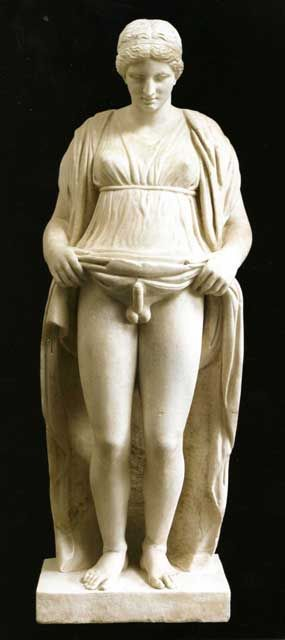
\includegraphics[width=7cm]{shock.jpg}};}%
\end{tikzpicture}
}

At this point let us try the new code and see the small improvements we have done.

\cxset{title font-color=spot!50}
\cxset{subtitle font-color/.store in=\subtitlefontcolor@cx}
\cxset{subtitle font-color=black!35}
\cxset{fashion image=shock.jpg}

% Image needs debugging, something is not capturing it.
\fashion

We have also used a different image and as you can observe with shock, our layout has lost its appeal, will
probably offend some people and the color scheme seems messed up. What we will probably have to do
is add a few more parameters, as well as measure the image’s dimension and implement different rules for
different aspect ratios. Try at this stage and use your own code to modify the layout.

\long\def\storyi{
         In antiquity men and women saw each other as different; 
         accordingly, they developed
        complex taxonomies (philosophical explanations) 
        for understanding anatomical,
        physiological, emotional, and rational differences. \par

Some of these differences seem
profoundly odd to us moderns. Modern discussions about erotic art have often concerned the place of women: to what
extent are they objects of social manipulation, to what extent can they be subjects?
}
\long\gdef\fashion#1{%
\begin{tikzpicture}

\if@debug
  \draw [help lines] (0,0) grid (18,-13);
  \draw[fill=red]  (0,0) circle (1.5pt) ;
  \draw[fill=red]  (0,-3) circle (1.5pt) ;
\else
\fi
% draw debug rectangles
\node[fashion, right, baseline] (x) at (0,1) {\LARGE\color{black!30}{before}\relax};
\draw[fill=red]  (0,1) circle (1.5pt) ;
\node[fashion, right=1sp] at (0,0) {\LARGE\color{black!20} \so\chaptername\relax};

\node[rectangle,draw, color=white, below right, fill=\fashionnumberbg@cx, text=white] at +(12,0) {\scalebox{2}{\HUGE \thechapter}};

% The title of the block
\node[fashion, text width=9cm,below right, yshift=-1pt] at (0,-3) {%
        { \sffamily\raggedleft
        \Huge\bfseries\color{\titlefontcolor@cx}#1\par}
         \bigskip
         \Large% 
         \centering
         \color{\subtitlefontcolor@cx}%
         \raggedleft
        \storyi\par}; 
        \IfFileExists{\fashionimage@cx}%   
           {\node at (12.5,-9) {\includegraphics[width=\imagewidth@cx]{\fashionimage@cx}};}%
           { \node at (12.5,-9) {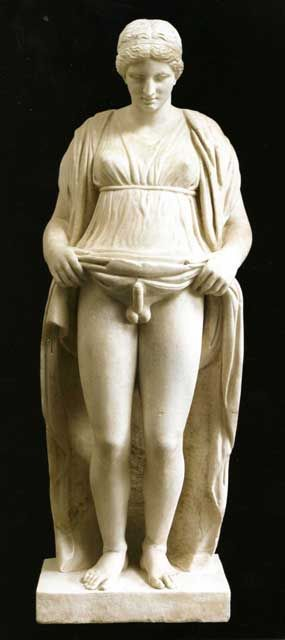
\includegraphics[width=7cm]{shock.jpg}};}%
\end{tikzpicture}
}

\fashion{SEXUALITY IN ANCIENT GREECE}
\makeatother
\bigskip

Using your document as a User Interface is  programming in a hostile environment. As mentioned
earlier, try pen and paper, it is the quickest way to get a layout right. Adding and removing text, in layouts such
as the one we have been developing is an essential part in getting the layout to get the layout aesthetics right.
Of course other people might have different taste than you and what you like would probably be distateful to other persons.
This is a common lamentation of Graphic Designers, who complain about the value systems of their Clients.

\subsection{Hooking onto LaTeX}

I think the layout is now much better and it has evolved to transform itself from a modern and colorful template to a more serious one, perhaps more appropriate for scientific work.

We have now won half the battle, the next battle is to hook into the |\section| or |\chapter| command using |\secdef|. As you might have noticed, the chapter number has not been incremented. We will need to also
add it to the Table of Contents and also get the indentation after the heading to work correctly. We do not want our users to have to worry about this and adding |\noindent|’s all over the place. At this point we will also 
add functions to add the chapter number and title to the Table of Contents. 

\makeatother

\makeatletter\@specialfalse\makeatother
\cxset{
         section font-family=tiresias,
         chapter numbering=arabic,
         chapter title align=none}
\chapter{More on Boxes: Using packages to automate boxing calculations and the drawing of borders.}
\thispagestyle{plain}
\pagestyle{headings}
\large

\section{Testing title values}
\makeatletter
\ExplSyntaxOn
title~display = \int_use:c {chapter_title_display} \\
chapter~title-display= \int_use:c {chapter_title_display} \\
title~display =\meaning\titledisplay@cx\\
chapter~title~text-align = \meaning\chaptertitletextalign@cx\\
%chapter~title~align = \tl_use:c {tl_chapter_title_align}
\meaning\chaptertitletextalign@cx
\makeatother
\ExplSyntaxOff

The boxing of contents is such an important concept in \tex and also in typography that it is worth examining some of the available packages that can be used.

Another elaborate package is Martin Scharrer’s package \pkgname{adjustbox}. The package uses numerous keys
to draw borders, adjust spacing and margins but also for the clipping of images. At the background the package uses and extends the \pkgname{graphicx} key value system.

This package allows to adjust general \latexe material in several ways using a key=value interface.
It got inspired by the interface of \cmd{\includegraphics} from the \pkg{graphicx} package.
 This package also loads the \pkg{trimclip} package which code was once included in this package.


 \subsection{Trimming and Clipping}
 
 Trimming and clipping is achieved by loading the \pkgname{trimclip}. This package forms part of the suit of packages developed by Martin Scharrer and or related to adjusting boxes and their sizes. The package allows for
 verbatim material as well. 
 
 \let\Macro\cmd
 
 The following keys allow content to be trimmed (i.e.\ the official size is made smaller, so the remaining material
 laps over the official boundaries) or clipped (overlapping material is not displayed).
 These keys come in different variants, where the lower-case keys represent the behavior of
 the corresponding \Macro\includegraphics keys. The corresponding macros (\Macro\trimbox, \Macro\clipbox, etc.)
 and environments (\env{trimbox}, \env{clipbox}, etc.) are included in the
 accompanying \pkg{trimclip} package and are explained in its manual.

 
 This key represents the original \option{trim} key of \Macro\includegraphics but accepts its value in different forms.
 Unlike most other keys it always acts on the original content independent in which order it is used with other keys.
 The key trims the given amounts from the lower left (ll) and the upper right (ur) corner of the box. This means that
 the amount \meta{llx} is trimmed from the left side, \meta{lly} from the bottom and \meta{urx} and \meta{ury} from the
 right and top of the box, respectively.
 If only one value is given it will be used for all four sites.
 If only two values are given the first one will be used for the left and right side (llx, urx) and the second for the
 bottom and top side (lly, ury).
 
\begin{texexample}{Example}{clipping}
\adjustbox{Clip=1, min width=8cm, center,}{This is some test}
\medskip

The untrimmed version is shown below
\medskip

\adjustbox{Clip=.1, min width=8cm, center,}{This is some test}%
\end{texexample}
 
\section{tcolorbox} 

\subsection{Breakable Boxes}

 \begin{verbatim}
 \begin{tcolorbox}[enhanced, breakable,
  colback=blue!5!white,colframe=blue!75!black,title=Breakable box,
  watermark color=white, watermark text=\Roman{tcbbreakpart}]
  \lipsum[1-18]
\end{tcolorbox}

	See \ref{test} for details and an example.
 \end{verbatim}
 
 
 

 
\cxset{style87/.style={
 chapter opening=any,
 chapter name=none,
 % positioning and float - inline is 0
 %  float right is 2
 number display=block,
 number float=right,
 number shape=starburst,
 numbering=Words,
 number spaceout=none,
 number font-size=huge,
 number font-weight=bold,
 number font-family=rmfamily,
 number font-shape=normal,
 number before=,
 number display=inline,
 number float=none,
% 
 number border-top-width=0pt,
 number border-right-width=0pt,
 number border-bottom-width=0pt,
 number border-left-width=0pt,
 number border-width=1pt,
%  
 number padding-left=0em,
 number padding-right=0.5em,
 number padding-top=0em,
 number padding-bottom=0pt,
  %number margin-top=, to do
 %number margin-left=0pt,  to create
 %
 number after=\par,
 number dot=,
 number position=rightname,
 number color=sweet,
 number background-color=white,
 %chapter name
 chapter display=block,
 chapter float=left,
 chapter shape=ellipse,
 chapter color=black,
 chapter background-color=sweet,
 chapter font-size= Huge,
 chapter font-weight=bfseries,
 chapter font-family=itshape,
 chapter before=,
 chapter spaceout=none,
 chapter after=,
 chapter margin-left=0cm,
 chapter margin-top=0pt,
 %
 chapter border-width=2pt,
 chapter border-top-width=1pt,
 chapter border-right-width=1pt,
 chapter border-bottom-width=1pt,
 chapter border-left-width=4pt,
% 
 chapter padding-left=20pt,
 chapter padding-right=20pt,
 chapter padding-top=20pt,
 chapter padding-bottom=10pt,
  %chapter title
 title font-family=rmfamily,
 title font-color=spot!80,                    %CHANGED
 title font-weight=bfseries,
 title font-size=huge,
 chapter title align=none,
 title margin-left=1cm,
 title margin-bottom=1.3cm,
 title margin-top=30pt,
 % title borders
 title border-width=0pt,
 title padding=0pt,
 title border-color=black!80,
 title border-top-color=spot!50,
 title border-top-width=2pt,
 title border-left-color=black!80,
 title border-left-width=2pt,
 title border-color=black!80,
 title padding-top=0pt,
 title padding-bottom=0pt,
 title padding-left=0pt,
 title padding-right=0pt,
 title border-right-color=spot!50,
 title border-right-width=2pt,
 title border-bottom-color=spot!50,
 title border-bottom-width=2pt,
 %
 chapter title align=left,
 chapter title text-align=left,
 chapter title width=0.8\textwidth,
 title before=,
 title after=,
 title display=block,
 title beforeskip=12pt,
 title afterskip=12pt,
 author block=false,
 section font-family=rmfamily,
 section font-size=LARGE,
 section font-weight=bfseries,
 section indent=0pt,
  section font-weight=mdseries,
 section align=left,
 subsubsection font-family=tiresias,
 subsubsection font-shape=upshape,
 subsubsection font-weight=mdseries,
 subsubsection align=flushleft,
 epigraph width=\dimexpr(\textwidth-2cm)\relax,
 epigraph align=center,
 epigraph text align=center,
 epigraph rule width=0pt,
 header style=plain}}
 
\cxset{style87}
\renewsection\renewsubsection\renewsubsubsection
\ExplSyntaxOff
\makeatother
\endinput

\makeatletter
\cxset{enumerate numberingi/.is choice,
  enumerate numberingi/.code={\renewcommand\theenumi {\csname#1\endcsname{enumi}}},
  enumerate numberingii/.code={\renewcommand\theenumii {\csname#1\endcsname{enumii}}},
  enumerate numberingiii/.code={\renewcommand\theenumiii {\csname#1\endcsname{enumiii}}},
  enumerate numberingiv/.code={\renewcommand\theenumiv {\csname#1\endcsname{enumiv}}},
  enumerate labeli punctuation/.store in=\enumeratepunctuationi@cx,
  enumerate labeli/.is choice,
  enumerate labeli/brackets/.code={\renewcommand\labelenumi{(\theenumi\enumeratepunctuationi@cx)}},
  enumerate labeli/square brackets/.code={\renewcommand\labelenumi{[\theenumi\enumeratepunctuationi@cx]}},
  enumerate labeli/right bracket/.code={\renewcommand\labelenumi{\theenumi\enumeratepunctuationi@cx)}},
  enumerate label left/.store in=\enumeratelabelleft@cx,
  enumerate label right/.code=\renewcommand\labelenumi{\enumeratelabelleft@cx\theenumi\enumeratepunctuationi@cx#1},
  enumerate leftmargini/.code={\setlength\leftmargini{#1}},
  enumerate leftmarginii/.code={\setlength\leftmarginii{#1}},
  enumerate leftmarginiii/.code={\setlength\leftmarginiii{#1}},
  enumerate leftmarginiv/.code={\setlength\leftmarginiv{#1}},
  listi topsep/.store in=\listitopsep@cx,
  listi partopsep/.store in=\listipartopsep@cx,
  listi itemsep/.store in=\listiitemsep@cx,
  listi parsep/.store in=\listiparsep@cx,
  listii topsep/.store in=\listiitopsep@cx,
  listii partopsep/.store in=\listiipartopsep@cx,
  listii itemsep/.store in=\listiiitemsep@cx,
  listii parsep/.store in=\listiiparsep@cx,
  listiii topsep/.store in=\listiiitopsep@cx,
  listiii partopsep/.store in=\listiiipartopsep@cx,
  listiii itemsep/.store in=\listiiiitemsep@cx,
  listiii parsep/.store in=\listiiiparsep@cx,
}
\cxset{compact1/.style={%
  enumerate numberingi=arabic,
  enumerate numberingii=alph,
  enumerate numberingiii=alph,
  enumerate numberingiv=roman,
  enumerate labeli punctuation=.,
  enumerate label left=,
  enumerate label right=,
  enumerate leftmargini=2.2em,
  enumerate leftmarginii=2.1em,
  enumerate leftmarginiii=1.5em,
  enumerate leftmarginiv=2em,
  listi topsep=8\p@ \@plus2\p@ \@minus\p@,
  listi itemsep=0\p@ \@plus2\p@ \@minus\p@,
  listi parsep=0\p@ \@plus2\p@ \@minus\p@,
  listii topsep=0\p@ \@plus2\p@ \@minus\p@,
  listii itemsep=0\p@ \@plus2\p@ \@minus\p@,
  listii parsep=0\p@ \@plus2\p@ \@minus\p@,
  listiii topsep=0\p@ \@plus2\p@ \@minus\p@,
  listiii itemsep=0\p@ \@plus2\p@ \@minus\p@,
  listiii parsep=0\p@ \@plus2\p@ \@minus\p@,
}}
\cxset{compact2/.style={%
  enumerate numberingi=alph,
  enumerate numberingii=roman,
  enumerate numberingiii=alph,
  enumerate numberingiv=roman,
  enumerate labeli punctuation=,
  enumerate label left=(,
  enumerate label right=),
  enumerate leftmargini=2.2em,
  enumerate leftmarginii=2.1em,
  enumerate leftmarginiii=1.5em,
  enumerate leftmarginiv=2em,
  listi topsep   = 8\p@ \@plus2\p@ \@minus\p@,
  listi itemsep = 0\p@ \@plus2\p@ \@minus\p@,
  listi parsep   = 0\p@ \@plus2\p@ \@minus\p@,
  listii topsep  = 0\p@ \@plus2\p@ \@minus\p@,
  listii itemsep= 0\p@ \@plus2\p@ \@minus\p@,
  listii parsep  = 0\p@ \@plus2\p@ \@minus\p@,
  listiii topsep = 0\p@ \@plus2\p@ \@minus\p@,
  listiii itemsep= 0\p@ \@plus2\p@ \@minus\p@,
  listiii parsep  = 0\p@ \@plus2\p@ \@minus\p@,
}}

\ExplSyntaxOn
\def\setenumerate#1{
\cxset{#1}
\def\@listi{%
           \leftmargin\leftmargini
            \parsep\listiparsep@cx
            \topsep\listitopsep@cx\relax
            \itemsep\listiitemsep@cx}
            
\def\@listii{\leftmargin\leftmarginii
            \parsep\listiiparsep@cx
            \topsep\listiitopsep@cx\relax
            \itemsep\listiiitemsep@cx}
            
\def\@listiii{\leftmargin\leftmarginiii
            \parsep\listiiiparsep@cx
            \topsep\listiiitopsep@cx\relax
            \itemsep\listiiiitemsep@cx}
}


\setenumerate{compact1}

\cxset{section align=left}
\cxset{section font-weight=bold}
\cxset{section font-family=sffamily} 
\cxset{section top rule=false,
          section bottom rule = false,
}
          
          
          
%  
\parindent0pt

\begin{minipage}{1.05\textwidth}
\vspace{\baselineskip}
\parindent0pt
\fboxrule0pt
{
\centering
\fbox{\centering
\begin{minipage}[t]{0.89\textwidth}
\centering
\begin{minipage}[t]{0.41\textwidth}
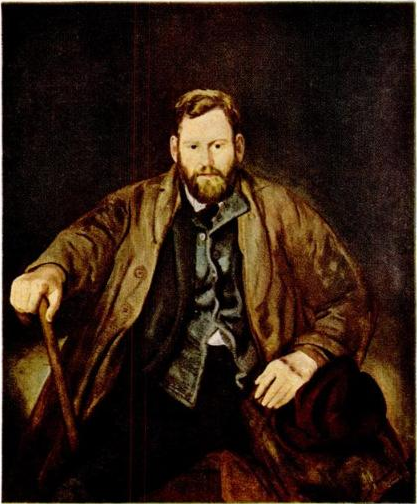
\includegraphics[width=1\textwidth]{threewomen01}\vspace*{-8pt}%
\captionof*{figure}{\noindent\footnotesize\textbf{WALDO PEIRCE}, a famous painting in his own right,
turned model for Bellows, posed for this impressive portrait in New York studio in 1920.}
\end{minipage}\hspace{0.5cm}
\begin{minipage}[t]{0.4\textwidth}
   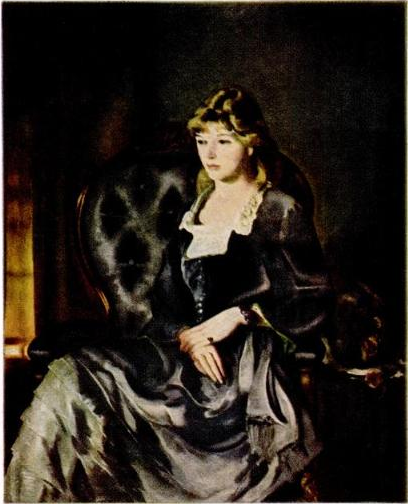
\includegraphics[width=1\textwidth]{threewomen02}\vspace*{-8pt}
    \captionof*{figure}{\noindent\footnotesize\textbf{MRS KATHERINE ROSEN,}
                 the daughter of Charles Rosen, he was an artist and neighbor of bellows, 
                 posed for this  meditative study in 1921.}
\end{minipage}
\end{minipage}
}}

\medskip

\fbox{\hskip-0.3cm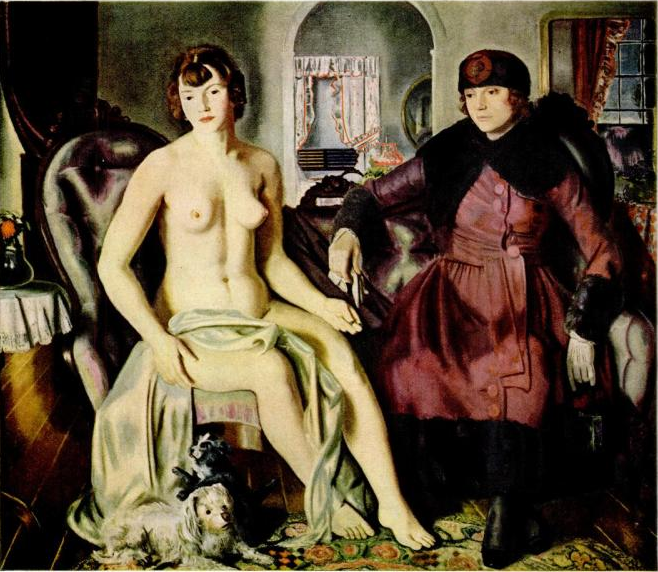
\includegraphics[width=1.03\textwidth]{twowomen-03}}\\[-27.5pt]
\setlength{\linewidth}{.95\textwidth}
\setlength{\columnsep}{8pt}
\begin{multicols}{2}
\noindent \footnotesize\textbf{TWO WOMEN,} portrays a professional model dressed and undressed. The range and richness of colors is unusual among Bellows' pictures. Bellows always had a horror of studio pictures and ``pretty nudes,'' rarely worked from professional models and never painted a still life.
\end{multicols}
\vfill

\captionof{figure}{Balancing three images on a page. Should the larger image be at the top or at the bottom?}
\end{minipage}

\newcommand\articleheading[1]{%
    \par
    \vspace*{2\baselineskip}
    \bgroup
    \LARGE\bf\textsf{\noindent #1}
    \egroup
   \vskip2\baselineskip
}
\clearpage

\begin{minipage}{\textwidth}
\includegraphics[width=\textwidth]{yaleartschool}

\articleheading{TRADITION AND TECHNIQUE AT YALE'S SCHOOL OF  FINE ARTS}

\end{minipage}
\begin{multicols}{3}
        \lettrine{A}{t Yale}\lorem \lipsum[1-3]
        \par
\end{multicols}

\newgeometry{top=0pt, left=0pt, right=0pt, top=0pt, bottom=2cm}
\pagebreak

\begin{minipage}{\textwidth}
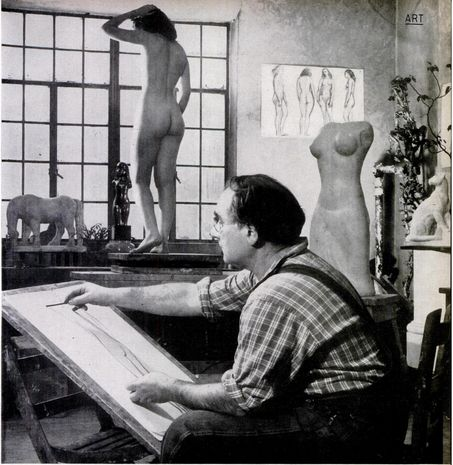
\includegraphics[width=\textwidth]{sculpture-lesson}\par
\vspace{\baselineskip}

\centerline{\HUGE\bfseries SCULPTURE LESSON}
\vspace{0.5\baselineskip}

\centerline{\LARGE\bfseries Noted arist shows how adventurous amateurs can model with clay }

\end{minipage}

{
\leftskip1cm\rightskip1cm\columnsep-1.3cm\par\leavevmode

\begin{multicols}{3}
        \lettrine{A}{t Yale} \lorem \lorem \lorem \lorem
        
\end{multicols}
}

\newgeometry{top=1.5cm,left=2cm,right=2cm,bottom=2cm}

\pagebreak





\lipsum[1]
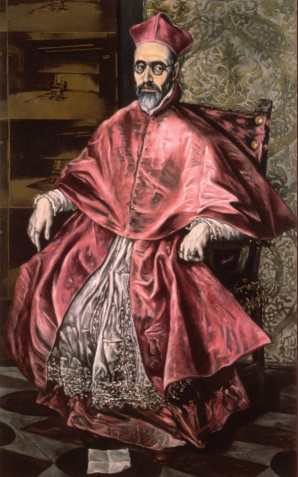
\includegraphics[height=0.8\textheight, width=\textwidth\relax]{nino}

This is a short caption test and this one is a long caption test.

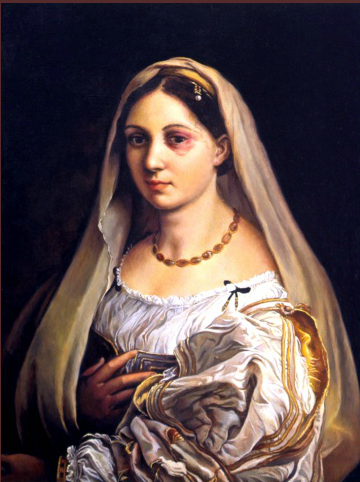
\includegraphics[width=\textheight, width=\textwidth]{woman}
Donna Velata.

\clearpage
\raggedbottom


\noindent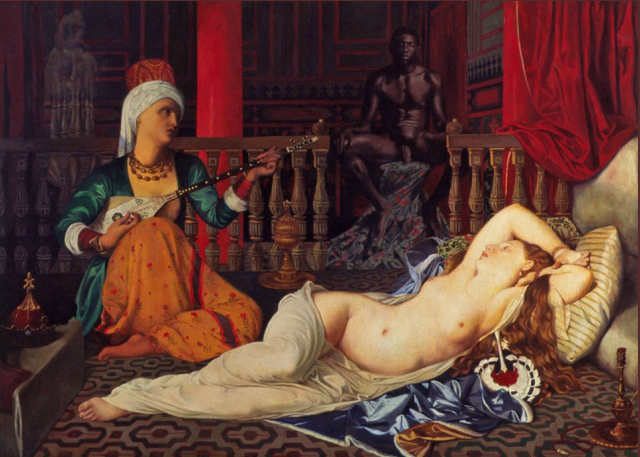
\includegraphics[width=\textwidth]{odalisque}%
This is a short caption test and this one is a long caption test.
\vspace*{2\baselineskip}


\begin{minipage}[t]{0.3\textwidth}
\vbox to -6cm{\noindent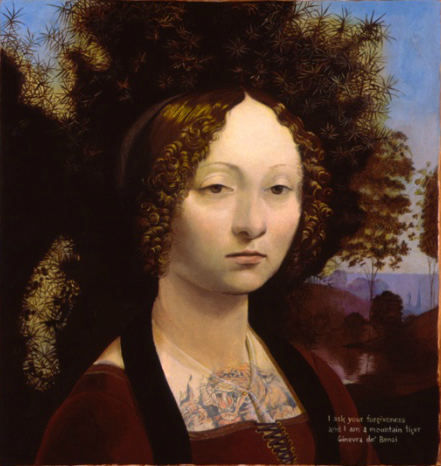
\includegraphics[width=0.98\textwidth]{ginerva}
This is a short caption test and this one is a long caption test.}
\end{minipage}%
\begin{minipage}[t]{.7\textwidth}%
\noindent\textbf{\Huge \hfill Kathleen Gilje\hskip0.1em\hfill}\\[2\baselineskip]
\end{minipage}


\leftskip0.41\textwidth

Lorem ipsum dolor sit amet, consectetur adipiscing elit. Etiam eu nunc dolor. Nam arcu nisi, hendrerit at facilisis et, aliquet sit amet massa. Aenean ullamcorper mi dolor. Sed ut urna vitae elit tristique varius tempus vitae orci. Maecenas tristique lectus vel enim posuere congue. Aliquam pellentesque nisl vel nunc iaculis dictum. Sed luctus, orci vehicula blandit rutrum, risus justo aliquet elit, id venenatis est libero nec sem. Sed varius molestie ante non fringilla.

Vestibulum ut mollis odio. Vivamus ut risus eu dolor laoreet viverra. Nullam elit erat, congue at placerat ut, posuere non diam. Suspendisse eget dui et mi varius bibendum at non orci. Morbi justo arcu, posuere non tempus at, vestibulum sit amet lorem. Class aptent taciti sociosqu ad litora torquent per conubia nostra, per inceptos himenaeos. Donec tempor dignissim tellus, vitae vestibulum tellus hendrerit tempus. Nullam varius justo sit amet risus semper non semper eros placerat. Integer eleifend ligula in est gravida ornare tincidunt velit tristique.


Donec vel erat a ipsum condimentum volutpat vel non odio. Vivamus non justo orci. Pellentesque ligula ipsum, vestibulum at molestie vel, mollis sed odio. Donec rhoncus, sem in auctor tincidunt, libero quam scelerisque urna, et volutpat purus magna ac nulla. Cras vel quam nec urna viverra ornare eu et nibh. Pellentesque tincidunt leo non odio varius vitae sollicitudin neque adipiscing. 

\section{Full Page Images}

\leftskip0pt\parindent1em

In euismod, enim a dictum pharetra, libero nibh tempor enim, vel fermentum justo justo eget sem. Integer convallis massa nec turpis volutpat tristique. Quisque fringilla volutpat sem porta elementum. Donec vel metus quis nisl venenatis vehicula ac quis est. Maecenas vulputate lacinia lacus quis porttitor. Aliquam consectetur consectetur metus eu bibendum. Lorem ipsum dolor sit amet, consectetur adipiscing elit. In sem mauris, mollis nec pulvinar posuere, facilisis quis turpis. Quisque vel laoreet mauris.

Quisque ultrices dignissim odio at malesuada. Duis euismod tellus nec ante porta vel ullamcorper orci semper. Vivamus in eros est. Etiam et pellentesque nisi. Sed faucibus dictum tortor vitae accumsan. Donec ante risus, ornare et iaculis eget, cursus at metus. Maecenas neque urna, rutrum sit amet lacinia non, accumsan nec tortor. Proin tempor dictum porta. Morbi luctus nulla et sapien elementum aliquam ut eget neque. Quisque lobortis eleifend lorem adipiscing semper. Quisque molestie magna lorem, non mollis est. Mauris urna arcu, pretium sed dignissim id, tempor accumsan massa



\noindent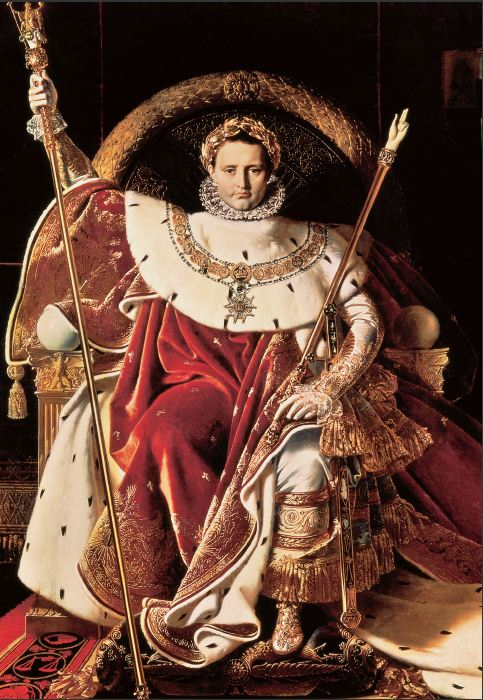
\includegraphics[width=\textwidth]{napoleon}
This is a short caption test and this one is a long caption test.



\clearpage
\newenvironment{kathleen}[1][b]{\def\placement{#1}\parindent0pt
}{}

\cxset{kathleen align/.is choice,
       kathleen align/top/.code=\xdef\kathleenplacement@cx{t},
       kathleen align/bottom/.code=\xdef\kathleenplacement@cx{b},
       kathleen align/center/.code=\xdef\kathleenplacement@cx{c},
       kathleen imagei/.code=\def\imagei{\includegraphics[width=\textwidth]{#1}\par},
 kathleen imageii/.code=\def\imageii{\includegraphics[width=\textwidth]{#1}\par},
kathleen imageiii/.code=\def\imageiii{\includegraphics[width=\textwidth]{#1}\par},
kathleen imageiv/.code=\def\imageiv{\includegraphics[width=\textwidth]{#1}\par},
kathleen imagev/.code=\def\imagev{\includegraphics[width=\textwidth]{#1}\par},
kathleen captioni/.code=\def\captioni{\captionof{figure}{#1}},
kathleen captionii/.code=\def\captionii{\captionof{figure}{#1}},
kathleen captioniii/.code=\def\captioniii{\captionof{figure}{#1}},
kathleen scale/.store in=\kathleenscale@cx
}

\long\def\printkathleen{\begin{kathleen}[t]
\begin{minipage}{\kathleenscale@cx\textwidth}
\begin{minipage}[\kathleenplacement@cx]{0.3\textwidth}
\vbox{}
\imagei
\captioni
\imageii
\captionii
\imageiii
\captioniii
\end{minipage}\hspace{1cm}
\begin{minipage}[\kathleenplacement@cx]{0.46\textwidth}
\vbox{}
\imageiv
\captionof{figure}{This is a short caption test and this one is a long caption test.}\par
\imagev
\captionof{figure}{This is a short caption test and this one is a long caption test.}
\end{minipage}
\end{minipage}
\end{kathleen}}

\begin{figure}
\cxset{kathleen align = top,
       kathleen imagei = ladyagnew,
       kathleen imageii = etta,
       kathleen imageiii = etta,
       kathleen imageiv = ladyagnew,
       kathleen imagev  = etta,
       kathleen captioni = {Al contrario di quanto si pensi, Lorem Ipsum non \`e semplicemente una sequenza casuale di caratteri. Risale ad un classico della letteratura latina del 45 AC.}, 
       kathleen captionii = {Finibus Bonorum et Malorum di Cicerone. Questo testo � un trattato su teorie di etica, molto popolare nel Rinascimento. La prima riga del Lorem Ipsum.},
       kathleen captioniii= This is a short caption.,
       kathleen scale = 1.1,
} 

\printkathleen

\caption{The Kathleen template page. It consists of five images and their caption text. Parameters can be set via a key value interface.}
\end{figure}
\clearpage

\cxset{kathleen align = top,
       kathleen imagei = ladyagnew,
       kathleen imageii = etta,
       kathleen imageiii = etta,
       kathleen imageiv = ladyagnew,
       kathleen imagev  = etta,
       kathleen captioni = {Al contrario di quanto si pensi, Lorem Ipsum non \`e semplicemente.}, 
       kathleen captionii = {Finibus Bonorum et Malorum di Cicerone. Questo testo � un trattato.},
       kathleen captioniii= This is a short caption.,
       kathleen scale = 0.7
} 

\cxset{kathleen align=bottom}




\begin{center}\printkathleen\par\label{kathleen}\end{center}

\newpage

\section{The Kathleen template} 

A lot of pages in image rich books have complicated settings for images.
These are difficult to manipulate and we provide here what we hope is
a better method. For example the Figure~\ref{kathleen} shows such a complex layout. This can be achieved by only filling in the template
values as shown below.

\begin{tcolorbox}
\begin{lstlisting}
\cxset{kathleen align = top,
       kathleen imagei = ladyagnew,
       kathleen imageii = etta,
       kathleen imageiii = etta,
       kathleen imageiv = ladyagnew,
       kathleen imagev  = etta,
       kathleen captioni = {Al contrario di quanto si pensi, Lorem Ipsum non \`e semplicemente una sequenza casuale di caratteri. Risale ad un classico della letteratura latina del 45 AC.}, 
       kathleen captionii = {Finibus Bonorum et Malorum di Cicerone. Questo testo � un trattato su teorie di etica, molto popolare nel Rinascimento. La prima riga del Lorem Ipsum.},
       kathleen captioniii= This is a short caption.,} 
\cxset{kathleen align=bottom,
       kathleen scale=.5}

\printkathleen

\end{lstlisting}
\end{tcolorbox}


\newgeometry{top=0pt,left=1cm,right=1cm,marginparsep=0pt}

\clearpage


\parindent0pt
\pagestyle{empty}

\fboxsep0pt
\fboxrule0pt

\vspace*{-1cm}
\begin{minipage}{1.05\textwidth}
\hskip-0.9cm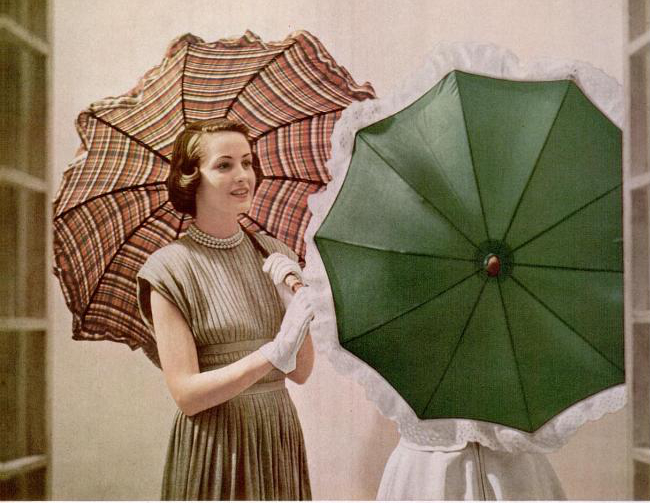
\includegraphics[width=1.03\textwidth]{parasol-05}\\[-27.5pt]
\setlength{\linewidth}{0.95\textwidth}
\setlength{\columnsep}{10pt}
\begin{multicols}{2}
\noindent \footnotesize\textbf{DESIGNED FOR CONTRAST} with the wearer's ensemble, these plaid  tafetta and green rayon parasols, are best sellers at Maey's in New York. Set of matching parasol and shoes, or
gloves, scarves or bags, are also available to give simple dresses
a custom appearance.
\end{multicols}
\vspace{-0.25cm}
\rule{1.5cm}{0pt}\fbox{
\begin{minipage}[t]{0.87\textwidth}
\begin{minipage}[t]{0.41\textwidth}
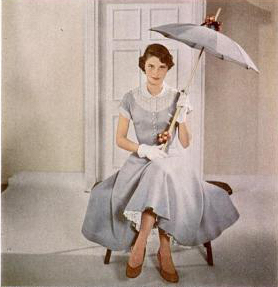
\includegraphics[width=1.03\textwidth]{parasol-06}\par%
\noindent \footnotesize\textbf{CHERRY ORNAMENTS} adorn handle and tip of this parasol, made by Jane Derby to go with the afternoon dress. Straight handles are very popular.
\end{minipage}\hspace{0.5cm}
\begin{minipage}[t]{0.4\textwidth}
   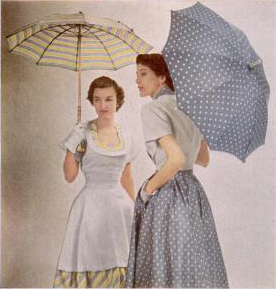
\includegraphics[width=1\textwidth]{parasol-07}\par
\noindent \footnotesize\textbf{MATCHING SETS} of afternoon dress
and parasol, and four-piece polka dot weekend dress and parasol,
both designed by Briganne.
\end{minipage}
\end{minipage}
}

\vfill

\captionof{figure}{Balancing three images on a page. Should the larger image be at the top or at the bottom?}
\end{minipage}




\begin{minipage}{\textwidth}
\begin{minipage}[b][\textheight][b]{.47\linewidth}
\vspace*{2cm}

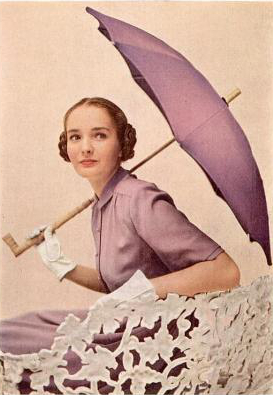
\includegraphics[width=\linewidth]{parasol-03}\par
\vspace{2\baselineskip}

\centerline{\bfseries\Huge Parasols}
\vspace{2\baselineskip}

\begin{quote}
\lipsum[2]
\end{quote}

\vfill

\textbf{SHOES AND PARASOL SET} in pink are herecombined with a dress, one of whose skirts is pink. Parasol is from New York's ``Uncle Sam'' parasol shop.
\end{minipage}\hspace*{1cm}
\begin{minipage}[b]{.53\linewidth}
\mbox{}
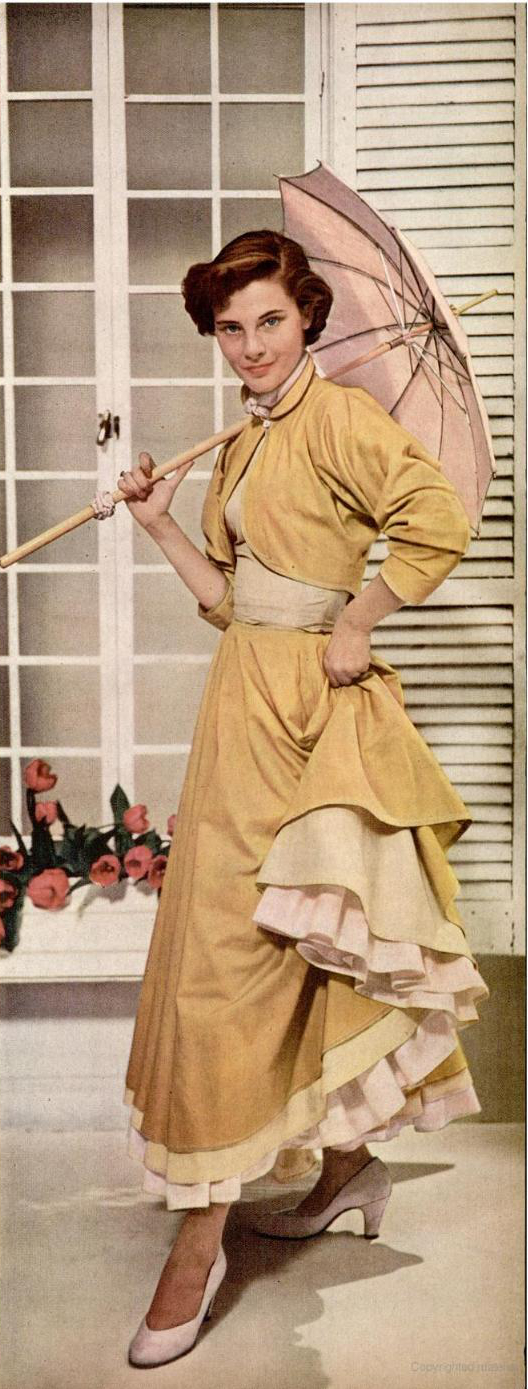
\includegraphics[width=\linewidth]{parasol-01}\par
\end{minipage}
\end{minipage}

\newgeometry{top=1.5cm,bottom=3cm,left=3.5cm,right=3.5cm}

\clearpage
%  \chapter{Image Pages}

\lipsum[1-5]

\clearpage

{
\parindent0pt
\pagestyle{empty}

\fboxsep0pt
\fboxrule0pt

\vspace*{-1cm}
\begin{minipage}{1.05\textwidth}
\hskip-0.9cm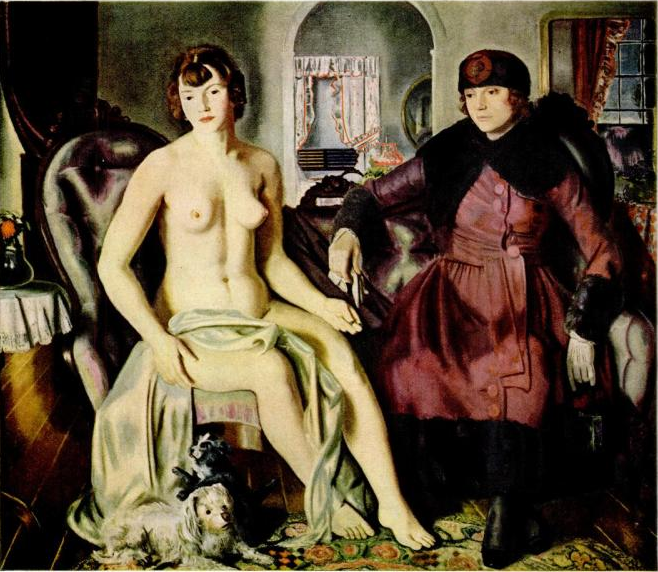
\includegraphics[width=1.03\textwidth]{twowomen-03}\\[-27.5pt]
\setlength{\linewidth}{0.95\textwidth}
\setlength{\columnsep}{10pt}
\begin{multicols}{2}
\noindent \footnotesize\textbf{TWO WOMEN,} portrays a professional model dressed and undressed. The range and richness of colors is unusual among Bellows' pictures. Bellows always had a horror of studio pictures and ``pretty nudes.'' He rarely worked from professional models and never painted a still life. This painting was published in Life Magazine.
\end{multicols}
\vspace{-0.25cm}
\rule{1.5cm}{0pt}\fbox{
\begin{minipage}[t]{0.87\textwidth}
\begin{minipage}[t]{0.41\textwidth}
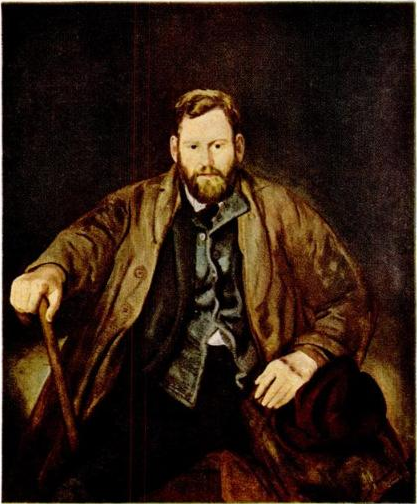
\includegraphics[width=1.03\textwidth]{threewomen01}\par\vspace*{-8pt}%
\captionof*{figure}{\noindent\footnotesize\textbf{WALDO PEIRCE}, a famous painting in his own right,
turned model for Bellows, posed for this impressive portrait in New York studio in 1920.}
\end{minipage}\hspace{0.5cm}
\begin{minipage}[t]{0.4\textwidth}
   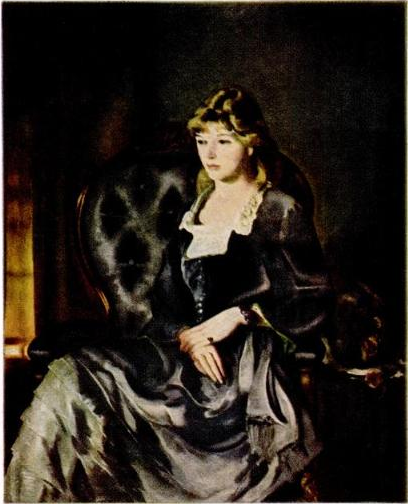
\includegraphics[width=1\textwidth]{threewomen02}\vspace*{-8pt}
    \captionof*{figure}{\noindent\footnotesize\textbf{Mrs Katherine Rosen,}
the daughter of Charles Rosen, he was an artist and neighbor of bellows, posed for this meditative study in 1921.}
\end{minipage}
\end{minipage}
}

\vfill

\captionof{figure}{Balancing three images on a page. Should the larger image be at the top or at the bottom?}
\end{minipage}
}


%   
%
\newgeometry{top=2cm, bottom=1cm, left=1cm, right=1cm,
               marginparsep=0cm, marginpar=0pt}
\makeatletter
\cxset{kroll scale/.store in = \scalekroll@cx,
       kroll left column width/.store in = \krollleftcolumnwidth@cx,
       kroll imagei/.store in = \krollimagei@cx,
       kroll imagei caption/.store in = \krollimageicaption@cx,
       kroll imageii/.store in = \krollimageii@cx,
       kroll imageii caption/.store in = \krollimageiicaption@cx,
       kroll left header/.store in = \krollleftheader@cx,
       kroll header/.store in = \krollheader@cx}

\cxset{kroll scale = 1,
       kroll left column width = .3\textwidth,
       kroll left header = Leon\\[15pt] Kroll,
       kroll imagei = krollportrait,
       kroll imagei caption = shows Kroll at 59. Says he. ``Painting is 
             fascinating'' even when motif my own mug.,
       kroll imageii = nudeback,
       kroll imageii caption = {NUDE  BACK  SHOWS   A  DANCER  WHOSE  BACK  SAYS  KROLL,  HAS  BEAUTIFUL  PLANES},
       kroll header = \scalebox{.97}{THE DEAN OF US NUDE-PAINTERS}
    }

\newenvironment{kroll}{%
\renewenvironment{leftcolumn}{%
   \minipage[b]{\krollleftcolumnwidth@cx}%
  }{\endminipage}\hspace*{0cm}%
 \renewenvironment{rightcolumn}{%
   \minipage[b]{.62\textwidth}%
  }{\endminipage}\hspace*{0cm}% 
\begin{minipage}{\scalekroll@cx\textwidth}%
 \noindent
  \begin{leftcolumn}%
   \MainHeader{\krollleftheader@cx}%
   \putimage[width=0.5\linewidth]{\krollimagei@cx}\par
   \aheader{\krollimageicaption@cx}%
\end{leftcolumn}\hfill%
\begin{rightcolumn}%
 \includegraphics[width=\linewidth]{\krollimageii@cx}%
 \onelinecaption{{\resizebox{\linewidth}{5.5pt}{\bfseries   \krollimageiicaption@cx}}\par}%
 \onelineheader{\krollheader@cx}%
 \begin{multicols}{2}}
{%
   \end{multicols}%
   \end{rightcolumn}%
   \end{minipage}} 
\makeatother



\begin{kroll}
 \lettrine{A}{t the} age of 63 when businessmen are thinking of retiring leon Kroll according to Life Magazine was having the busiest time of his life, just doing what comes naturally.  \lorem
\end{kroll}

\cxset{kroll scale = 1,
       kroll left column width = .3\textwidth,
       kroll left header = Cooling\\Water\\ Systems\vskip5pt
                          {\bfseries \Large \lorem},
       kroll imagei = industrial,
       kroll imagei caption = shows Kroll at 59. Says he. ``Painting is 
                                    fascinating'' even when motif my own mug.,
        kroll imageii = industrial,
       kroll imageii caption = {NUDE  BACK  SHOWS   A  DANCER  WHOSE  BACK  SAYS  KROLL,  HAS  BEAUTIFUL  PLANES},
       kroll header = \scalebox{1}{\hfill HVAC CHILLED WATER SYSTEMS \hfill}
    }


\begin{kroll}
 \lettrine{A}{t the} age of 63 when businessmen are thinking of retiring leon Kroll according to Life Magazine was having the busiest time of his life, just doing what comes naturally.  \lorem \the\pagetotal
\end{kroll}

\restoregeometry

%  \cxset{section color=teal}
%  \newpage

\makeatletter

\@specialtrue

\cxset{steward,
  chapter name=chapter,
  numbering=arabic,
  custom= stewart,
  offsety=0cm,
  image=sweepers,
  texti={Lists are essential elements of any document style and perhaps the most troublesome to get right.
         In this chapter we discuss the construction of lists and offer a key value interface.},
  textii={The Chapter discusses in detail the construction of lists. It reviews the mechanisms offered
          by LaTeX and outlines a key value approach to building lists. We define a standard interface that does not
          interfere with the original commands. The three standard list styles \textit{enumerate, itemize} and \textit{description} are redesigned to accept a key value interface. The photograph is Lewis Hine's which noted: ``Ivey Mill Company, Hickory, N.C. Some doffers and sweepers. Plenty of them.'' Location: Hickory, Catawba County Date: November 1908. Photographs like this were used by Hine to campaign against child labour.
         }
}

\chapter{Standard \LaTeX\ Lists}

\tcbset{width=\linewidth,arc=1mm,before=\bigskip,after=\medskip,left=8mm}

The general parameters affecting a general list is shown in the  diagram  below\footnote{Produced using the \texttt{layouts} package.}. LaTeX offers three general list structures, enumerate, itemize and description.
\begin{figure}[hp]
\listdiagram
\caption{Layout of an \texttt{enumerate} list} \label{fig:lstenum}
\end{figure}

\section{Package usage}

List are set using setenumerate, setitemize, setdescription. It is also possible to create new list structures, which will be explained a bit later on.

\newpage
\section{The description list environment}
Unlike the enumerate and itemize environment, the description list environment is defined in the book class.
The environment is defined as:

\begin{tcolorbox}
\begin{lstlisting}
\newenvironment{description}
               {\list{}{\labelwidth\z@ \itemindent-\leftmargin
                        \let\makelabel\descriptionlabel}}
               {\endlist}
\newcommand*\descriptionlabel[1]{\hspace\labelsep\labelcolor@cx
                                \normalfont\bfseries #1}
\end{lstlisting}
\end{tcolorbox}

What is important to notice here is that all the standard list parameters are left essentially unchanged. The only item that is affected is \lstinline{\makelabel}, which is redefined in \lstinline{description} label.


We can define a number of keys for ease of formatting such descriptions lists rather than each time redefining them.


\begin{tcolorbox}[title=Basic description list keys]
\begin{lstlisting}
\cxset{
 description label font-size/.store in=\descriptionlabelfontsize@cx,
 description label font-weight/.store in=\descriptionlabelfontweight@cx,
 description label font-family/.store in=\descriptionlabelfontfamily@cx,
 description label font-shape/.store in=\descriptionfontshape@cx,
 description label color/.store in=\descriptionlabelcolor@cx,
 description label sep/.store in=\descriptionlabelsep@cx,
 description label width/.store in=\descriptionlabelwidth@cx,
 description margin left/.store in=\descriptionmarginleft@cx,
 description margin right/.store in=\descriptionmarginright@cx,
 description item indent/.store in=\descriptionitemindent@cx,
 list parindent/.store in=\descriptionlistparindent@cx,
}
\end{lstlisting}
\end{tcolorbox}

\cxset{
 description label font-size/.store in=\descriptionlabelfontsize@cx,
 description label font-weight/.store in=\descriptionlabelfontweight@cx,
 description label font-family/.store in=\descriptionlabelfontfamily@cx,
 description label font-shape/.store in=\descriptionlabelfontshape@cx,
 description label color/.store in=\descriptionlabelcolor@cx,
 description label sep/.store in=\descriptionlabelsep@cx,
 description label width/.store in=\descriptionlabelwidth@cx,
 description margin left/.store in=\descriptionmarginleft@cx,
 description margin right/.store in=\descriptionmarginright@cx,
 description item indent/.store in=\descriptionitemindent@cx,
 list parindent/.store in=\descriptionlistparindent@cx,
}

We also define a macro \lstinline{\setdescription} as a helper macro to assist in changing settings at any point in a document.

\begin{tcolorbox}[title=Basic description list keys]
\begin{lstlisting}
\def\setdescription#1{%
\cxset{#1}%
\renewenvironment{description}%
{\list{}{\listparindent\descriptionlistparindent@cx%
                       \leftmargin=\descriptionmarginleft@cx%
                       \rightmargin=\descriptionmarginright@cx%
                       \itemindent\descriptionitemindent@cx%
                       \labelwidth\descriptionlabelwidth@cx%
                       \labelsep=\descriptionlabelsep@cx%
                       \let\makelabel\descriptionlabel}}%
               {\endlist}%
%
\renewcommand\descriptionlabel[1]{%
  \fboxrule0pt\fboxsep0pt%
  \hspace\descriptionlabelsep@cx%
  \fbox{\color{\descriptionlabelcolor@cx}%
  \normalfont\bfseries\raggedleft##1\thickspace%
}}%
}
\end{lstlisting}
\end{tcolorbox}


\def\setdescription#1{%
\cxset{#1}%
\renewenvironment{description}%
{\list{}{\listparindent\descriptionlistparindent@cx%
                       \leftmargin=\descriptionmarginleft@cx%
                       \rightmargin=\descriptionmarginright@cx%
                       \itemindent\descriptionitemindent@cx%
                       \labelwidth\descriptionlabelwidth@cx%
                       \labelsep=\descriptionlabelsep@cx%
                       \let\makelabel\descriptionlabel}}%
               {\endlist}%
%
\renewcommand\descriptionlabel[1]{%
  \fboxrule0pt\fboxsep0pt%
  \hspace\descriptionlabelsep@cx%
  \fbox{\color{\descriptionlabelcolor@cx}%
  \normalfont\bfseries\raggedleft##1\thickspace%
}}%
}
\setdescription{%
 description label font-size=\normalfont,
 description label font-weight=\bfseries,
 description label font-family=\sffamily,
 description label font-shape=\itshape,
 description label color=purple,
 description label sep=0sp\relax,
 description label width=100pt,
 description margin left=20pt,
 description margin right=20pt,
 description item indent=90pt,
 list parindent=1em,
}

\section{Creating new description like environments}

The macro \lstinline{\newdescriptionenvironment} can be used to redefine new description like environments.

\begin{tcblisting}{title=Example: define new description list environment}
\def\newdescriptionenvironment#1#2{%
\cxset{#2}%
\newenvironment{#1}%
{\list{}{\listparindent\descriptionlistparindent@cx%
                       \leftmargin=\descriptionmarginleft@cx%
                       \rightmargin=\descriptionmarginright@cx%
                       \itemindent\descriptionitemindent@cx%
                       \labelwidth\descriptionlabelwidth@cx%
                       \labelsep=\descriptionlabelsep@cx%
                       \let\makelabel\descriptionlabel}}%
               {\endlist}%
%
\renewcommand\descriptionlabel[1]{%
  \fboxrule0pt\fboxsep0pt%
  \hspace\descriptionlabelsep@cx%
  \fbox{\color{\descriptionlabelcolor@cx}%
  \descriptionlabelfontsize@cx%
  \descriptionlabelfontweight@cx%
  \descriptionlabelfontfamily@cx%
  \descriptionlabelfontshape@cx%
  \hbox to \labelwidth{\hfill##1}%
}}%
}
\newdescriptionenvironment{orangedescription}{
 description label font-size=\normalfont,
 description label font-weight=\bfseries,
 description label font-family=\sffamily,
 description label font-shape=\itshape,
 description label color=orange,
 description label sep=3.5pt\relax,
 description label width=40pt,
 description margin left=50pt,
 description margin right=20pt,
 description item indent=-2.5pt,
 list parindent=1em,
}
The \texttt{orangedescription} environment in action.
\begin{orangedescription}
 \item[One] \lorem
 \item[Two] \lorem
 \item[Three] \lorem
\end{orangedescription}
\end{tcblisting}

\newpage

\section{Example: redefining a description list}
We will now develop a description environment, that can be useful for the documentation of packages to describe options. We will use a description list as the basis of the environment. We define the following key values.

\begin{description}
\item[description label font-size]This is the first item.
\item[description label font-weight]This is the second item. \lipsum*[1]
\item[description label font-family] This is the font family.
\item[description label font-shape] This is the font family.
\item[description label color] This is the font family.
\item[description label sep] The space between the description label and the description text.
\item [description label width] The space between the description label and the description text.
[description margin left] The space between the list indentation and the left margin.
\lipsum*[3]
\end{description}


\section{Enumerated lists}


\begin{enumerate}
\item one
\item two
\item three
\end{enumerate}

Enumerated (numbered) list environments are characterized by numbering. They use a variety of fields and counters as shown in table.

\subsection{Vertical skips}

By default LaTeX adds vertical skips, as shown in figure 1. The definition of these skips is influenced by the font size and are defined in the \texttt{bk10.clo} files, hence hard to find and change. Each level of the list has its own definition as \lstinline{\@listi}.

\bigskip
\tcbset{width=\linewidth,arc=1mm,before=\bigskip,left=8mm}

\begin{tcolorbox}[title=Extract from bk10.clo]
\begin{lstlisting}
\def\@listi{\leftmargin\leftmargini
            \parsep 4\p@ \@plus2\p@ \@minus\p@
            \topsep 8\p@ \@plus2\p@ \@minus4\p@
            \itemsep4\p@ \@plus2\p@ \@minus\p@}
\let\@listI\@listi
\@listi
\def\@listii {\leftmargin\leftmarginii
              \labelwidth\leftmarginii
              \advance\labelwidth-\labelsep
              \topsep    4\p@ \@plus2\p@ \@minus\p@
              \parsep    2\p@ \@plus\p@  \@minus\p@
              \itemsep   \parsep}
\def\@listiii{\leftmargin\leftmarginiii
              \labelwidth\leftmarginiii
              \advance\labelwidth-\labelsep
              \topsep    2\p@ \@plus\p@\@minus\p@
              \parsep    \z@
              \partopsep \p@ \@plus\z@ \@minus\p@
              \itemsep   \topsep}
\def\@listiv {\leftmargin\leftmarginiv
              \labelwidth\leftmarginiv
              \advance\labelwidth-\labelsep}
\def\@listv  {\leftmargin\leftmarginv
              \labelwidth\leftmarginv
              \advance\labelwidth-\labelsep}
\def\@listvi {\leftmargin\leftmarginvi
              \labelwidth\leftmarginvi
              \advance\labelwidth-\labelsep}
\end{lstlisting}
\end{tcolorbox}


\cxset{enumerate numberingi/.is choice,
  enumerate numberingi/.code={\renewcommand\theenumi {\csname#1\endcsname{enumi}}},
  enumerate numberingii/.code={\renewcommand\theenumii {\csname#1\endcsname{enumii}}},
  enumerate numberingiii/.code={\renewcommand\theenumiii {\csname#1\endcsname{enumiii}}},
  enumerate numberingiv/.code={\renewcommand\theenumiv {\csname#1\endcsname{enumiv}}},
  enumerate labeli punctuation/.store in=\enumeratepunctuationi@cx,
  enumerate labeli/.is choice,
  enumerate labeli/brackets/.code={\renewcommand\labelenumi{(\theenumi\enumeratepunctuationi@cx)}},
  enumerate labeli/square brackets/.code={\renewcommand\labelenumi{[\theenumi\enumeratepunctuationi@cx]}},
  enumerate labeli/right bracket/.code={\renewcommand\labelenumi{\theenumi\enumeratepunctuationi@cx)}},
  enumerate label left/.store in=\enumeratelabelleft@cx,
  enumerate label right/.code=\renewcommand\labelenumi{\enumeratelabelleft@cx\theenumi\enumeratepunctuationi@cx#1},
  enumerate leftmargini/.code={\setlength\leftmargini{#1}},
  enumerate leftmarginii/.code={\setlength\leftmarginii{#1}},
  enumerate leftmarginiii/.code={\setlength\leftmarginiii{#1}},
  enumerate leftmarginiv/.code={\setlength\leftmarginiv{#1}},
  listi topsep/.store in=\listitopsep@cx,
  listi partopsep/.store in=\listipartopsep@cx,
  listi itemsep/.store in=\listiitemsep@cx,
  listi parsep/.store in=\listiparsep@cx,
  listii topsep/.store in=\listiitopsep@cx,
  listii partopsep/.store in=\listiipartopsep@cx,
  listii itemsep/.store in=\listiiitemsep@cx,
  listii parsep/.store in=\listiiparsep@cx,
  listiii topsep/.store in=\listiiitopsep@cx,
  listiii partopsep/.store in=\listiiipartopsep@cx,
  listiii itemsep/.store in=\listiiiitemsep@cx,
  listiii parsep/.store in=\listiiiparsep@cx,
}

\cxset{compact1/.style={%
  enumerate numberingi=arabic,
  enumerate numberingii=alph,
  enumerate numberingiii=alph,
  enumerate numberingiv=roman,
  enumerate labeli punctuation=.,
  enumerate label left=,
  enumerate label right=,
  enumerate leftmargini=2.2em,
  enumerate leftmarginii=2.1em,
  enumerate leftmarginiii=1.5em,
  enumerate leftmarginiv=2em,
  listi topsep=8\p@ \@plus2\p@ \@minus\p@,
  listi itemsep=0\p@ \@plus2\p@ \@minus\p@,
  listi parsep=0\p@ \@plus2\p@ \@minus\p@,
  listii topsep=0\p@ \@plus2\p@ \@minus\p@,
  listii itemsep=0\p@ \@plus2\p@ \@minus\p@,
  listii parsep=0\p@ \@plus2\p@ \@minus\p@,
  listiii topsep=0\p@ \@plus2\p@ \@minus\p@,
  listiii itemsep=0\p@ \@plus2\p@ \@minus\p@,
  listiii parsep=0\p@ \@plus2\p@ \@minus\p@,
}}

\cxset{compact2/.style={%
  enumerate numberingi=alph,
  enumerate numberingii=roman,
  enumerate numberingiii=alph,
  enumerate numberingiv=roman,
  enumerate labeli punctuation=,
  enumerate label left=(,
  enumerate label right=),
  enumerate leftmargini=2.2em,
  enumerate leftmarginii=2.1em,
  enumerate leftmarginiii=1.5em,
  enumerate leftmarginiv=2em,
  listi topsep=8\p@ \@plus2\p@ \@minus\p@,
  listi itemsep=0\p@ \@plus2\p@ \@minus\p@,
  listi parsep=0\p@ \@plus2\p@ \@minus\p@,
  listii topsep=0\p@ \@plus2\p@ \@minus\p@,
  listii itemsep=0\p@ \@plus2\p@ \@minus\p@,
  listii parsep=0\p@ \@plus2\p@ \@minus\p@,
  listiii topsep=0\p@ \@plus2\p@ \@minus\p@,
  listiii itemsep=0\p@ \@plus2\p@ \@minus\p@,
  listiii parsep=0\p@ \@plus2\p@ \@minus\p@,
}}


\def\setenumerate#1{
\cxset{#1}
\def\@listi{\leftmargin\leftmargini
            \parsep\listiparsep@cx
            \topsep\listitopsep@cx\relax
            \itemsep\listiitemsep@cx}
\def\@listii{\leftmargin\leftmarginii
            \parsep\listiiparsep@cx
            \topsep\listiitopsep@cx\relax
            \itemsep\listiiitemsep@cx}
\def\@listiii{\leftmargin\leftmarginiii
            \parsep\listiiiparsep@cx
            \topsep\listiiitopsep@cx\relax
            \itemsep\listiiiitemsep@cx}
}

\setenumerate{compact1}


The list can be viewed here:

\begin{enumerate}
\item Level i
      \begin{enumerate}
       \item Level ii
          \begin{enumerate}
            \item Level iii
              \begin{enumerate}
                \item Level iv. \lipsum*[1]
              \end{enumerate}
          \end{enumerate}
      \end{enumerate}
\end{enumerate}


\begin{tcblisting}{title=Example with style \textit{compact2}}

\cxset{compact2/.style={%
  enumerate numberingi=alph,
  enumerate numberingii=roman,
  enumerate numberingiii=alph,
  enumerate numberingiv=roman,
  enumerate labeli punctuation=,
  enumerate label left=(,
  enumerate label right=),
  enumerate leftmargini=2.2em,
  enumerate leftmarginii=2.1em,
  enumerate leftmarginiii=1.5em,
  enumerate leftmarginiv=2em,
  listi topsep=8\p@ \@plus2\p@ \@minus\p@,
  listi itemsep=0\p@ \@plus2\p@ \@minus\p@,
  listi parsep=0\p@ \@plus2\p@ \@minus\p@,
  listii topsep=0\p@ \@plus2\p@ \@minus\p@,
  listii itemsep=0\p@ \@plus2\p@ \@minus\p@,
  listii parsep=0\p@ \@plus2\p@ \@minus\p@,
  listiii topsep=0\p@ \@plus2\p@ \@minus\p@,
  listiii itemsep=0\p@ \@plus2\p@ \@minus\p@,
  listiii parsep=0\p@ \@plus2\p@ \@minus\p@,
}}
\setenumerate{compact2}
\begin{enumerate}
\item Does this project actually merit the use of the Minor Works Form or Intermediate Form instead of their `grown up' relatives?
\item Do the number of PC or prime cost items mean that it would be more desirable to use a re-measurable form?
\item Is this a contract which merits the production of full scale bills
of quantities or is something more standardised going to suffice?
\end{enumerate}
\end{tcblisting}

As you will observe the numbering in the above example has been enclosed in round brackets, using:

\begin{tcolorbox}
\begin{lstlisting}
  enumerate label left=(,
  enumerate label right=),
\end{lstlisting}
\end{tcolorbox}

The next example is from the \textit{LaTeX Companion}. In example~\ref{ex:companion}, the first-level list elements are decorated with the section sign (\S) as a prefix and a period as a suffix (omitted in references). We will
define this as a style named \textit{paragraphsymbol} for the lack of any better name. This style can sometimes be found in legal texts.

\begin{texexample}{Paragraph symbols in enumerate}{ex:companion}
\cxset{paragraphsymbol/.style={%
  enumerate numberingi=arabic,
  enumerate labeli punctuation=.,
  enumerate label left=\S,
  enumerate label right=,
}}
\setenumerate{paragraphsymbol}
\begin{enumerate}
\item \lorem
\item \lorem
\item \lorem
\end{enumerate}
\end{texexample}

\section{Creating enumerated environments}

New enumerated environments cab be created by using the macro \lstinline{\newenumeratedenvironment}. Keys are set as either styles or individually.

\def\newenumeratedenvironment#1#2{%
 \expandafter\def\csname#1\endcsname{%
 \cxset{#2}
 \ifnum \@enumdepth >\thr@@\@toodeep\else
 \advance\@enumdepth\@ne
 \edef\@enumctr{enum\romannumeral\the\@enumdepth}%
 \expandafter
 \list
 \csname label\@enumctr\endcsname
 {\usecounter\@enumctr\def\makelabel####1{\hss\llap{####1}}}%
 \fi}
 \expandafter\let\csname end#1\endcsname=\endlist
}


\begin{texexample}{An enumerated list factory}{}
\newenumeratedenvironment{paragraphsymbol}{
  enumerate numberingi=roman,
  enumerate labeli punctuation=.,
  enumerate label left={\textcolor{purple}{\P}},
  enumerate label right=,
}
\begin{paragraphsymbol}
\item \lorem
\item \lorem
\item \lorem
      \begin{itemize}
        \item This is bullets
      \end{itemize}
\end{paragraphsymbol}
\end{texexample}


\newpage
\section{Setup keys for enumerate lists}
\begin{description}
\item [enumerate numberingi] Sets the numbering style of the list at level $n$. Valid values are \textit{Alph, alph, arabic, Roman, roman, WORDS, words}.
\end{description}

\clearpage

\section{Itemized lists}

The itemized \LaTeX\ lists are similar to those for the enumerated lists. However they are somehow simpler as there is no need for counters.

\bigskip
\begin{tcolorbox}[width=\linewidth,arc=2mm,title=Default \LaTeX\ parameters for itemized lists]
\begin{lstlisting}
\newcommand\labelitemi{\textbullet}
\newcommand\labelitemii{\normalfont\bfseries \textendash}
\newcommand\labelitemiii{\textasteriskcentered}
\newcommand\labelitemiv{\textperiodcentered}
\end{lstlisting}
\end{tcolorbox}

\cxset{
 labelitemi/.code=\def\labelitemi{#1},
 labelitemii/.code=\def\labelitemii{#1},
 labelitemiii/.code=\def\labelitemiii{#1},
 labelitemiv/.code=\def\labelitemiv{#1},
}

\cxset{
 labelitemi={{\color{red}\ding{"E4}}},
 labelitemii=\textendash,
 labelitemiii=\textasteriskcentered,
 labelitemiv=\textperiodcentered,
}



\begin{itemize}
\item Level i
      \begin{itemize}
       \item Level ii
          \begin{itemize}
            \item Level iii
              \begin{itemize}
                \item Level iv. \lipsum*[1]
              \end{itemize}
          \end{itemize}
      \end{itemize}
\end{itemize}

\cxset{red/.style={
 labelitemi={{\color{green}\ding{'64}}},
 labelitemii=\color{red}\textendash,
 labelitemiii=\textasteriskcentered,
 labelitemiv=\textperiodcentered,
}}

Now that we have managed to abstract the itemized environment we can generate a new environment factory.

\def\newitemizedenvironment#1#2{
\expandafter\def\csname#1\endcsname{%
 \cxset{#2}%
 \ifnum \@itemdepth >\thr@@\@toodeep\else
 \advance\@itemdepth\@ne
 \edef\@itemitem{labelitem\romannumeral\the\@itemdepth}%
 \expandafter
 \list
 \csname\@itemitem\endcsname
 {\def\makelabel####1{\hss\llap{####1}}}%
 \fi}
 \expandafter\let\csname end#1\endcsname=\endlist
}

\newitemizedenvironment{reditemize}{red}


\begin{reditemize}
\item Test.
   \begin{reditemize}
    \item test.
   \end{reditemize}
\end{reditemize}

\begin{itemize}
\item Level i
      \begin{itemize}
       \item Level ii
          \begin{itemize}
            \item Level iii
              \begin{itemize}
                \item Level iv. \lipsum*[1]
              \end{itemize}
          \end{itemize}
      \end{itemize}
\end{itemize}


\section{Itemized lists with ding symbols}

So far we have used both standard symbols as well as those provided by the pifont that offers numerous,
dingbang symbols. The pifont package also offers environments to do that more easily.


\begin{texexample}{dinglist}{}
\begin{dinglist}{"E4}
\item The first item. \item The second
item in the list.
\end{dinglist}
\end{texexample}

\begin{dingautolist}{'300}
\item The first item in the list.\label{lst:a}
\item The second item in the list.\label{lst:b}
\item The third item in the list.\label{lst:c}
\end{dingautolist}

%  \cxset{style13,
       chapter toc=true,
       toc image={}}
\chapter{The Special Environments Quotation and Quote}

\precis{This Chapter and the next discuss the use of quotation marks and quotations and quotes in text, there use and the techniques and packages to improve their management. }
\label{quotations}


\begin{figure}[p]
\centering
\fbox{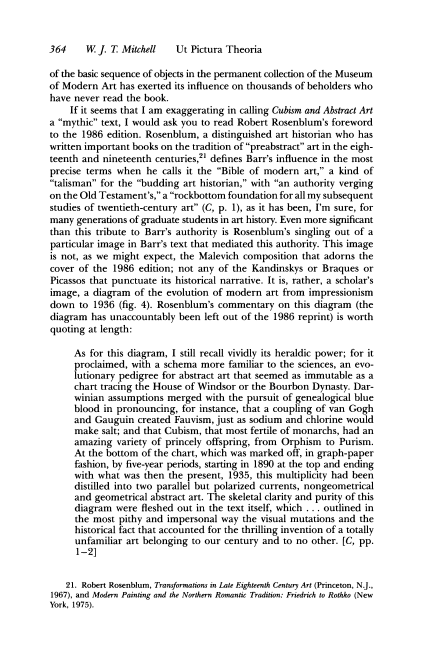
\includegraphics[width=0.9\linewidth]{./images/quotations-01.png}}
\caption{Many books have quotes flushed right.}
\label{frightquotation}
\end{figure}

\begin{figure}[p]
\centering
\fbox{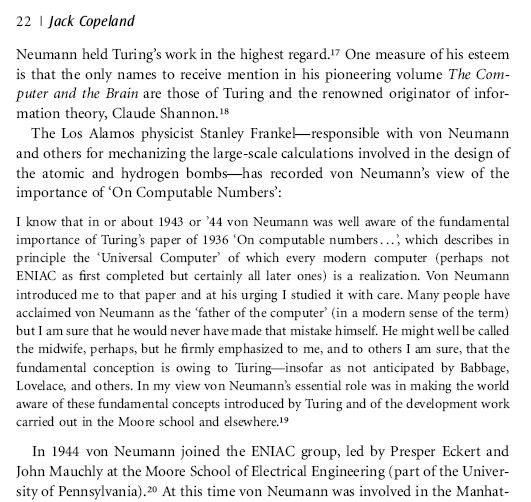
\includegraphics[width=0.9\linewidth]{./images/full-width-quotation.jpg}}
\caption[Sample quotation.]{Other books have the quotations full width, but in smaller font as shown above. the extract is from \textit{The Essential Turing}, Edited by B. Jack Copeland and  published by the Oxford University Press, 2004. }
\label{fullwidthquotation}
\end{figure}


\section{Quotation}

In the standard \LaTeXe\ classes the quotation and quote environment are defined by making use of the list environment. The main difference between the quotation and the quote environment is that the first line of the former is indented. The key value interface for the quotation environment is shown below and a similar one exists for the quotation environment:


\let\quotation\oquotation
\begin{quotation}
\lipsum[1]
\end{quotation}

The standard classes offer a very similar enevironment with the only difference the first line is not indented and is illustrated below:

\begin{quote}
\lipsum[1]
\end{quote}


\section{Key-value interface}\index{quotation!keys}


\begin{key}{/phd/ quote above = \meta{dim}} The space to leave at the top of the quote environment. This is a skip dimension. 
\end{key}

\begin{key}{/phd/ quote below = \meta{dim}} The space to leave at the bottom of the quote environment. This is a skip dimension. 
\end{key}
\begin{key}{/phd/ quote parindent = \meta{dim}} The paragraph indentation, set to 0pt for the quote environment by
\latex.
\end{key}
\begin{key}{/phd/ quote parsep = \meta{dim}} The paragraph separation, normally set to 1pt.
\end{key}
\begin{key}{/phd/ quote left margin = \meta{dim}} The indentation from the left margin.
\end{key}
\begin{key}{/phd/ quote right margin = \meta{dim}} The indentation from the right margin.
\end{key}

\begin{key}{/phd/ quote font-name = \meta{fontcmd}} Set a different font. Defaults to document 
\end{key}
\index{quotation!example}
\begin{tcblisting}{title=Quotation environment example,width=\textwidth}
\bgroup
\setquotation{%
  quotation above=36pt,
  quotation left margin=30pt,
  quotation right margin=0pt,
  quotation parsep=10pt,
  quotation font-size=,
  quotation parindent=1em,
  quotation font-name=\arial,
}
\lorem

\begin{quotation}
\lipsum[2-3]
\end{quotation}
\egroup
\end{tcblisting}

\section{Quote}
This is the quote environment:
\begin{quote}
\lipsum[1-2]
\end{quote}


\section{Some commonly used styles}

Besides the centered quotation \fref{fullwidthquotation} shows a style
common in Oxford University Publications. This one is from \textit{The Essential Turing}, Edited by B. Jack Copeland and  published by the Oxford University Press, 2004. Perhaps indicative of the efforts of academic publications to keep costs down quotations are set at full width, but in smaller font. They both look good and keep the cost down by reducing the amount of paper required to print the book.

\topline

Von Neumann gave his engineers `On Computable Numbers' to read when, in
1946, he established his own project to build a stored-programme computer at
the Institute for Advanced Study.\textsuperscript{22} Julian Bigelow, von Neumann's chief engineer,
recollected:
\vspace*{-20pt}

\cxset{quotation example/.style={
  quotation above=0pt,
  quotation left margin=0pt,
  quotation right margin=0pt,
  quotation parsep=10pt,
  quotation font-size=\small\color{blue},
  quotation parindent=1em,
  quotation font-name=\arial,
}}

\cxset{quotation turing/.style={
  quotation above=0pt,
  quotation left margin=0pt,
  quotation right margin=0pt,
  quotation parsep=10pt,
  quotation font-size=\small,
  quotation parindent=1em,
  quotation font-name=\pan,
}}

\cxset{quotation theme/.code = \setquotation{quotation #1},
       quotation style/.code = \setquotation{quotation #1}}



\cxset{quotation theme = example}
\begin{quotation}

The person who really\ldots pushed the whole Weld ahead was von Neumann, because he
understood logically what [the stored-programme concept] meant in a deeper way than
anybody else\ldots The reason he understood it is because, among other things, he understood
a good deal of the mathematical logic which was implied by the idea, due to the
work of A. M. Turing\ldots in 1936-1937\ldots Turing's [universal] machine does not sound
much like a modern computer today, but nevertheless it was. It was the germinal
idea\ldots So\ldots [von Neumann] saw\ldots that \textsc{[ENIAC]} was just the first step, and that great
improvement would come.\textsuperscript{23}
\end{quotation}

\bottomline

Personally I like this style, especially for books that have a lot
of lengthy citations such as typically found in the humanities and
scientific fields.

\section{Theming}

To make things easier for the designer and to enable easy re-use of
styles we defined a theme key. You first define your keys via
the \cs{cxset} command and then you call it normally using the 
theme. You can extend it, if you like to use sub-themes, such as 
quotation theme |quotation theme = example teal|. 

\begin{teX}
\cxset{quotation example/.style={
  quotation above=0pt,
  quotation left margin=0pt,
  quotation right margin=0pt,
  quotation parsep=10pt,
  quotation font-size=\small,
  quotation parindent=1em,
  quotation font-name=\arial,
}}
\cxset{quotation theme = example}
\end{teX}

\cxset{quotation font-size=\large,
       quote font-size=\large}








%  
\cxset{lineskip/.code=\setlength\lineskip{#1},
       lineskip/.default=1pt,
          normallineskip/.code=\setlength\normallineskip{#1},
          parindent/.code=\setlength\parindent{#1},
          parskip/.code=\setlength\parskip{#1},
          text-indent/.code=\setlength\parindent{#1},
          baselinestretch/.code=\renewcommand\baselinestretch{#1},
          single spacing/.code=\singlespacing,
          single spacing/.default=\singlespacing,
          double spacing/.code=\doublespacing}

\cxset{lineskip=1pt,
          normallineskip=1pt,
          parindent=1em,
          parskip=1pt,
          text-indent=1em,
          baselinestretch={},
          single spacing}

\makeatletter\@specialtrue\makeatother
\cxset{steward,
  numbering=arabic,
  custom=stewart,
  offsety=0cm,
  image={./images/hine05.jpg},
  texti={When Lamport designed the original \LaTeX\ sectioning commands, limitations of computer power forced him to restrict the abstraction of complicated chapter layouts. With current tools available improvements are much easier to program.},
  textii={In this chapter we discuss a method that allows the production of fancy chapter headings and formatting, based on a set of key values. Central  to this process is the separation of content from presentation.
We also discuss the basic formatting tools that are available and how one can modify them to mould new book designs.
 }
}
\cxset{chapter opening=left}

\chapter{General Settings}

\section{Introduction}

Here we define and set general paragraph settings. The parameters which control \TeX's behaviour when typesetting paragraphs can receive a bit of a tweak here. We also describe a set of options to handle parameters that can influence grid typesetting. This is especially important for two or more column typesetting. The commands act only on the text within a grouped environment. They do not affect captions or footnotes. Use anything over \emph{single spacing} with care, as books are meant to be single spaced.  



\section{Controlling inter-line spacing}
\index{line spacing}
Interline spacing traditionally has been controlled using the \pkgname{setspace} or by setting appropriate primitive \tex commands. The \pkgname{phd} loads the |setspace| package and then provides parameterized commands for setting styles. 

\begin{key}{/chapter/single spacing} 
	The Lineskip parameter emulates \TeX's \cmd{\parindent} command.
\end{key}
\begin{key}{/chapter/one half spacing} 
	The Lineskip parameter emulates \TeX's \cmd{\parindent} command.
\end{key}
\begin{key}{/chapter/double spacing} 
	Sets the document line-spacing to double.
\end{key}

If you want to use larger inter-line spacing in a document, you can change its value by putting the

\CMDI{\linespread}\meta{factor} Use |\linespread{1.3}| for "one and a half" line spacing, and |\linespread{1.6}| for "double" line spacing. Normally the lines are not spread, so the default line spread factor is~1.

The setspace package allows more fine-grained control over line spacing. To set "one and a half" line spacing document-wide, but not where it is usually unnecessary (e.g. footnotes, captions):

\begin{teXXX}
\usepackage{setspace}
%\singlespacing
\onehalfspacing
%\doublespacing
%\setstretch{1.1}
\end{teXXX}

The |phd| package provides the settings

\begin{key}{/chapter/single spacing}
We use the \pkgname{setspace} to effect the desired line spread effect.
\end{key}


These command offer little value over the normal \TeX\ macros other than keeping the interface, uniform. One can also extend the interface to cover CSS style commands:

\begin{verbatim}
\cxset{text-indent=50pt}

\cxset{double spacing}
\lipsum*[1]

\cxset{single spacing}
\lipsum*[1]
\end{verbatim}



\subsection{Parameters controlling paragraphs}\index{Paragraphs!controlling parameters}
The parameters \cs{lineskip} and \cs{normallineskip} influence \TeX\ when two lines come two close.
\medskip



\begin{key}{/chapter/lineskip=1pt} 
	The Lineskip parameter emulates \TeX's \cmd{\lineskip} command.
\end{key}

\begin{key}{/chapter/normallineskip=\marg{dim}} 
	The normallineskip parameter emulates \TeX's \cmd{\normallineskip} command.
\end{key}

\begin{key}{/chapter/lineskiplimit=\marg{dim}} 
	The Lineskip parameter emulates \TeX's \cmd{\lineskiplimit} command.
\end{key}

\begin{key}{/chapter/parindent=\marg{dim}} 
	The Lineskip parameter emulates \TeX's \cmd{\parindent} command.
\end{key}

\keyval{parindent}{\marg{dim}}{Paragraph indentation.}
\keyval{text-indent}{\marg{dim}}{Alias for \cs{parindent}.}
\keyval{parskip}{\marg{dim}}{Spacing between paragraphs.}


Another advantage, the package offers a few pre-configured styles, just setting a style to latex will revert everything back to latex.

\section{Technical discussion}

Most classes, including the standard \LaTeXe\ classes as well as packages attempting to achieve a grid typesetting try define a text height that is a multiple of \cs{baselineskip}. This way they give little opportunity to TeX to adjust the vertical glue to achieve a flush bottom.

\section{Dropcaps and Lettrines}\index{Lettrine!basic typesetting}

Dropcaps or lettrines are those letters that start paragraphs with a fancy larger letter. The class uses a parameterized version of the lettrine package of Daniel Flipo. Lettrine letters are easily typed and produced, but they are notoriously difficult to get right and no-one seems to agree on settings. These settings depend on the font the sizing of the text and the personal taste of the book interior designer. As I don't profess to be one, I have done what I think Knuth have done (just studied existing sources) allowed programming hooks and provided defaults as close as possible to the originals.



%  
%%% DOCUMENATION MACROS
%% note becareful with styles here

\thispagestyle{plain}
\cxset{image=breakerboys, custom=stewart}
\chapter{Documentation}


\section{Documentation macros}

When developing this package the need arose to define a number of documentation macros. I have used heavily macros and ideas present in the doc package, pgf documentation, biblatex documentation  and tcolorbox and for which I am grateful to their respective authors. The major change was to adopt the macros to use different fonts and colors and to use these from a list of key values defined at document level. More about this later. General package user documentation as opposed to package documentation that can be achieved using the doc/docstrip system requires that macros and environments be developed for the following:

\begin{enumerate}
\item Macros for command documentation.
\item Environments for commands and options.
\item Latex examples that need to be executed within the document as well as described.
\end{enumerate}

\subsection{Color management}
One of the first requirements for redefining some of the standard doc commands is the need to use color easily, hence we will try and define a certain amount of keys for colors.

Just a bit of a refresher, to define colors we use, either the \cs{definecolor} or the \cs{colorlet} commands.

\emphasis{definecolor,colorlet}
\begin{tcolorbox}
\begin{lstlisting}
% used for hyperlinks
\definecolor{Hyperlink}{rgb}{0.281,0.275,0.485}
\colorlet{thehyperlink}{theblue}
\end{lstlisting}
\end{tcolorbox}

We use a semantic approach, where the colors are first defined with a mnemonic command such as {\bfseries\textcolor{theblue}{theblue}} and then we define a semantic command such as the\cs{option} that lets the color to the option command. This sort of double entry has proved useful in navigating through the dozen of the commands that I needed for this documentation.

%\definecolor{theblue} {rgb}{0.02,0.04,0.48}
%\definecolor{thered}  {rgb}{0.65,0.04,0.07}
%\definecolor{thegreen}{rgb}{0.06,0.44,0.08}
%\definecolor{thelightgreen}{rgb}{0.06,0.44,0.06}
%\definecolor{thegrey} {gray}{0.5}
%\definecolor{thegrey} {gray}{0.5}
%\definecolor{theshade}{gray}{0.94}
%\definecolor{theframe}{gray}{0.75}
%\definecolor{thecream}{rgb}{1,0.95,0.4}
%\definecolor{spot}{rgb}{0,0.2,0.6}
%\definecolor{boxframe}{gray}{0.8}
%\definecolor{boxfill}{rgb}{0.95,0.95,0.99}
%\definecolor{theoption}{rgb}{0.118,0.546,0.222}
%\definecolor{themacro}{rgb}{0.784,0.06,0.176}
%\definecolor{ExampleFrame}{rgb}{0.628,0.705,0.942}
%\definecolor{ExampleBack}{rgb}{0.963,0.971,0.994}
%\definecolor{Hyperlink}{rgb}{0.281,0.275,0.485}
%\colorlet{thehyperlink}{theblue}
%\newcommand*{\defaultcolor}{\color{black}}
%\newcommand*{\spotcolor}{\color{spot}}

\subsection{Semantic color names}
\begin{marglist}
\item [\option{theoption}] Coloring of options in margin lists.
\item [\option{themacro}] Coloring of command macros \cs{foo}.
\item [\option{hyperlink}] If we use the \texttt{hyperref} package a number of colors need to be defined for links.
\end{marglist}

\subsection{Named colors}
Standard colors that we provide are:
\begin{marglist}
\item [\textcolor{theblue}{theblue}] This color is used mainly for options.
\item [\textcolor{thered}{thered}] The color mostly used for macro commands and keys.
\item [\textcolor{thegreen}{thegreen}] used for environments.
\item [\textcolor{thelightgreen}{thelightgreen}] Used for margin lists.
\item [\textcolor{thegray}{thegray}] Used as a background to the listings.
\item [\colorbox{thegrey}{\color{white}thegrey}] Alias for the gray to satisfy both sides of the Atlantic and as I sometimes don't remeber which is which.
\item [\colorbox{theshade}{theshade}] Another slightly lighter shade.
\end{marglist}



\begin{marglist}
\item [\cs{cs}] \cs{cs}\marg{text} Prints a command.
\item [\cs{cmd}] \cmd{\cmd}\marg{\cmd{\foo}} Prints a command.
\item[\cs{meta}] \marg{macro|text} Prints an argument
\end{marglist}




\section{Lists for documentation}



The environment \env{marglist}
\begin{marglist}
\item[testing]\lorem
\item [test]\lorem
\end{marglist}

\env{keymarginlist}This environment is suitable for listing keys, set-in the margin.

\begin{keymarglist}
\item[bibliography] The term <bibliography>, also available as \cmd{bibname}.
\item[references] The term <references>, also available as \cmd{refname}.
\item[shorthands] The term <list of shorthands> or <list of abbreviations>, also available as \cmd{losname}.
\end{keymarglist}


\env{argumentlist} This environment is suitable for listing macro arguments and their explanations.

\newenvironment*{argumentlist}[1]
  {\list{}{%
     \settowidth{\labelwidth}{\displayverbfont#1}%
     \setlength{\labelsep}{1em}%
     \setlength{\leftmargin}{\labelwidth}%
     \addtolength{\leftmargin}{\labelsep}%
     \setlength{\itemsep}{0pt}%
     \renewcommand*{\makelabel}[1]{\displayverbfont##1\hss}}}
  {\endlist}

\begin{argumentlist}{00}
\item[\#1] The last names. If a name consists of a single part only (for example, <Aristotle>), this part will be treated as the last name.
\item[\#2] The last names, given as initials.
\item[\#3] The first names. This argument also includes all middle names.
\end{argumentlist}

\begin{tabular}{ll}
\env{marglist} & description list\\
\end{tabular}


\section{Future improvements}

Future improvements will involve defining additional environments and styles to integrate styles to those provided for chapters. Treat the code so far as a proof of concept experiment. It is also possible to improve on the code by utilizing some of the common packages.


%
% \cxset{style13}
% \cxset{section align=left,
%        section color=teal,
%         section font-weight=bold,
%         title font-family=sfamily,
%         title font-shape=upshape,
%         subsection indent=0pt,
%         subsection font-shape=upshape}
% \renewsection
% \renewsubsection
%
% \part{IMPLEMENTATION}
% 
% \chapter{Implementation Strategy}
%
% The implementation is divided into parts. Perhaps cutting,
% these parts into smaller packages might have been a better
% choice, but as the aim of the package is to minimize
% the loading of packages and rather let |phd| to handle
% this, it made more sense to me, anyway to keep everything
% together.
% 	
%
% \begin{description}
%
%   \item[The Package Manager] This section is responsible 
%       for pre-loading a packages, resolving conflicts and 
%       providing a number of interface commands.
%
%  \item[The Sectioning Layouts Manager] This section manages 
%       the design of complex layouts for sectioning comands.
%
%  \item [The Image Page Manager] This section manages the design of 
%       pages that consist primarily of images and complex
%		page layouts.
%
%  \item[Common Macros] We provide a number of predefined commands
%		for macros that us and other people found useful.
%
%  \item[MWE] The package generates a large number
%		of Minimum Working Examples that we use for testing. 
%		Most of them can also used as examples for training 
%		or self-study.
%
% \end{description}
%
% \section{The Package Manager}
%
% The basic requirement for the Package Manager is to load
% an adequate number of packages to enable the typesetting
% of a diverse number of large documents without requiring
% additional packages to be loaded by typical groups of
% authors.
%
% \section{Preliminaries}
%
%    Standard file identification. We first announce the package 
%	 and require that it be used with \LaTeX2e. 
%
%    \begin{macrocode}
\NeedsTeXFormat{LaTeX2e}
[1994/12/01]%
\ProvidesPackage{phd}[2013/2/26 v1.0 less preamble (YL)]%
%    \end{macrocode}
%
% Load \pkg{fixltx2e} to update \LaTeX2e for various fixes.
% 
%    \begin{macrocode}
\RequirePackage{fixltx2e}                
%    \end{macrocode}
% 
%
% \chapter{Package Management} 
%  
% In order to keep track of all the packages and keys we require a
% number of macros will be defined first.
% 
% Each of the packages used by this document is loaded conditionally.
% However, it might be nice to know if we have a complete set.  So we
% define |\ifcomplete| which starts true, but gets set to false if any
% package is missing. Some code is necessary in order to manage 
% the complexity.
% I am idebted to the source of |symbols.tex| for some of the macros.
% There are a number of symbols (e.g., \cmd{\Square}) that are defined by      
% multiple packages.  In order to typeset all the variants in this       
% document, we have to give glyph a unique name.  
% To do that, we define  
% \cs{savesymbol{XXX}}, which renames a symbol from \cs{XXX} to \cmd{origXXX}, and    
% \cmd{restoresymbols{yyy}{XXX}}, which renames \cmd{origXXX} back to \cmd{XXX} and     
% defines a new command, |\yyyXXX|, which corresponds to the most recently 
% loaded version of |\XXX|.                                                
%                                                                        
% This implementation of \savesymbol and \restoresymbol was copied from  
% the |savesym| package, which started with symbol.tex's old definitions   
% of those macros and improved upon them.  However, \renamerobustsymbol  
% and |\ifnotsavedsym| are from  the list of |symbols| documentation.                                
%                                                                        
% 
%
% \begin{macro}{\savesymbol}
%    \begin{macrocode}
\newcommand*{\savesymbol}[1]{%
  \expandafter\let\csname orig#1\expandafter\endcsname\csname#1\endcsname
  \expandafter\let\csname #1\endcsname\relax
}
%    \end{macrocode}
% \end{macro}
%    

% \begin{macro}{\restoresymbols}
% 	Restore a previously saved symbol, and rename the current one.
%    \begin{macrocode}
\newcommand*{\restoresymbol}[2]{%
  \expandafter\global\expandafter\let\csname#1#2\expandafter\endcsname%
    \csname#2\endcsname
  \expandafter\global\expandafter\let\csname#2\expandafter\endcsname%
    \csname orig#2\endcsname
}
%    \end{macrocode}  
% \end{macro}
 
% Rename a robust command.
%    \begin{macrocode}
\newcommand*{\renamerobustsymbol}[2]{%
  \expandafter\let\expandafter\origrealcommand
    \csname #2\space\endcsname
  \expandafter\global\expandafter\let\csname#1#2\endcsname=\origrealcommand
}
%    \end{macrocode}
% Test if a symbol is not saved.
%    \begin{macrocode}
\def\ifnotsavedsym@helper#1#2!{\expandafter\ifx\csname orig#2\endcsname\relax}
\newcommand*{\ifnotsavedsym}[1]{%
  \expandafter\ifnotsavedsym@helper\string#1!%
}
%    \end{macrocode}
% \begin{macro}{\ifcomplete}
%    \begin{macrocode}
\newif\ifcomplete
%    \end{macrocode}
% \end{macro}    
%    
% For debugging purposes we define a switch that enables us to toggle
% on and off the loading of packages.
% 
%    \begin{macrocode}
\newif\ifloadpackages
\loadpackagestrue
%    \end{macrocode}
%    
% |\IfStyFileExists*| is just like |\IfFileExists|, except that it appends
% ".sty" to its first argument.  |\IfStyFileExists| is the same as
% |\IfStyFileExists*|, but it additionally adds its first argument to a list
% (|\missingpkgs|) and marks the document as incomplete (with
% |\completefalse|) if the |.sty| file doesn't exist.
% 
% \begin{macro}{\missingpkgs}
% \begin{macro}{\foundpkgs}
%   \begin{macrocode}
\newcommand{\missingpkgs}{}
\newcommand{\foundpkgs}{}
\newcommand{\if@sty@file@exists@star}[3]{%
  \ifloadpackages
    \IfFileExists{#1.sty}{#2}{#3}%
  \else
    #3%
  \fi
}
\newcommand{\if@sty@file@exists}[3]{%
  \ifloadpackages
    \IfFileExists{#1.sty}%
                 {#2\@cons\foundpkgs{{#1}}}%
                 {#3\completefalse\@cons\missingpkgs{{#1}}}%
  \else
    #3\completefalse\@cons\missingpkgs{{#1}}%
  \fi
}
\newcommand{\IfStyFileExists}{%
  \@ifstar{\if@sty@file@exists@star}{\if@sty@file@exists}%
}
%    \end{macrocode}
% \end{macro}
% \end{macro}
%
% \subsection{Utility macros for displaying symbols and fonts}
%
% In the sections that follow, we use a number of utilities for
% displaying fonts and utilities in tables and figures, we collect
% them here and make them available to the user for document
% use.
%
% \begin{macro}{\symbols}
% \begin{macro}{\endsymbols}
%    \begin{macrocode}
% From stmarysrd symbols package
% A very convenient command to typeset symbols.
% Much preferable than tables. Slight modifications to
% make it a bit more clear
\def\symbols{\flushleft}
\def\endsymbols{\endflushleft}
\def\dosymbol#1{%
   \leavevmode\hbox to .33\textwidth{%
    \hbox to 1.2em%
    {\hss$#1$\hfil}%
   \footnotesize\texttt{\string#1}\hss}%
   \penalty10}
%    \end{macrocode}
% \end{macro}
% \end{macro}
%
% \symbols
% \dosymbol{\Square} \dosymbol{\square} \dosymbol{\Diamond} \dosymbol{\diamond} \(\dosymbol{\symbol{60}}\)
% \endsymbols
%   
% \section{Best practices macros} 
% 
% We load a few packages for fixes and errors and |nag| if outdated packages are used.
% Modify to suit your requirements.  
% Package management is a bit complex to avoid errors
% with options.
%To find out if a package has already been loaded, use
%|\@ifpackageloaded|\meta{package}\meta{true}\meta{false}.
%|\@ifpackagelater| To find out if a package has already been loaded with a version more recent
%|\@ifclasslater| than version, use |\@ifpackagelater|\meta{hpackagei}\meta{hversioni}\meta{true}\meta{hfalsei}.
%|\@ifpackagewith| To find out if a package has already been loaded with at least the options
%hoptionsi, use |\@ifpackagewith|\meta{package}\meta{options}\meta{true}\meta{false}. 
%There exists one package that can't be tested with the above commands: the
%fontenc package pretends that it was never loaded to allow for repeated reloading
%with different options (see ltoutenc.dtx for details).
%
% 
% We include the following two packages to provide the standard 
% fixes for \LaTeX2e\ and the |nag| package to provide some guidance
% as to good
% practices. We set the |nag| keys to |orthodox| and |l2tabu.|
% \url{http://tex.stackexchange.com/questions/19264/techniques-and-packages-to-keep-up-with-good-practices?rq=1}
% and \href{http://stackoverflow.com/questions/193298/best-practices-in-latex}{best practices in LaTeX.}
%

% We load |pgf| and |pgfkeys| early as we need them for key management.
% 
% \begin{environment}{etex}
%    \begin{macrocode}
\RequirePackage{etex}
%    \end{macrocode}
% \end{environment}
%
%    \begin{macrocode}
\RequirePackage{pgf,pgfkeys}               % before onlyasmath
\def\cx@optionlist{}
\def\cxuselibrary#1{\cxset{library/.cd,#1}}
%
% The library is added by inputting the file and setting the path accordingly.
\def\cx@add@library#1#2{%
  \cxset{library/#1/.code={\@ifundefined{cxlibrary@#1@loaded}{\input #2}{}}}%
  \DeclareOption{#1}{\edef\cx@optionlist{\cx@optionlist,#1}}%
}
% We create a family for keys, unimaginatively named chapter. This might
% change in the future.
\pgfkeys{/chapter/.is family}
\newcommand\cxset{\pgfqkeys{/chapter }} %Notice this is pgf q keys
%
%

\cxset{nag keys/.store in =\nagkeys@cx,
       onlyamsmath keys/.store in=\onlyamsmathkeys@cx,
       xcolor keys/.store in=\xcolorkeys@cx}
%        
%
%%
%% This is file `settings.tex',
%% generated with the docstrip utility.
%%
%% The original source files were:
%%
%% phd.dtx  (with options: `settings')
%% ----------------------------------------------------------------
%% phd --- A package to beautify documents.
%% E-mail: yannislaz@gmail.com
%% Released under the LaTeX Project Public License v1.3c or later
%% See http://www.latex-project.org/lppl.txt
%% ----------------------------------------------------------------
%% 








%% Some settings
\cxset{nag keys = {l2tabu,%
                   orthodox}}
\cxset{onlyamsmath keys = {warning}}

\endinput
%%
%% End of file `settings.tex'.
 % experimental
%\cxset{nag keys = {l2tabu,%
%                   orthodox,%
%                   %
%                  }}
%    \end{macrocode}
%
% \begin{macro}{xcolor}
% 	For |xcolor| we try and load as many pre-defined colornames as
% 	possible.
%    \begin{macrocode}
\cxset{xcolor keys={fixpdftex,xtable,usenames,dvipsnames,
                    svgnames,x11names}}                     
% Set amsmath keys
%
%    \end{macrocode}
% \end{macro}
%
%    \begin{macrocode}
%\PassOptionsToPackage{\nagkeys@cx}{nag}
%\RequirePackage{nag}   
%    \end{macrocode}

%
%
% \begin{macro}{onlyasmath}
% The package |onlyasmath| also provides errors for deprecated math
% commands like using |$$|\ldots|$$| which can result in unwanted spaces
% being introduced in the typsetting of the document. The recommended 
% way is to use |\[|\ldots|\]|. The package was developed by Harold Harders
% and although targetted for class writers one might as well use it directly.
% 
%    \begin{macrocode}

%\PassOptionsToPackage{\onlyamsmathkeys@cx}{onlyamsmath}
%\RequirePackage{onlyamsmath} 
\RequirePackage{microtype}
%    \end{macrocode}
% \end{macro}
%
% I prefer to issue an error rather than a warning to instill good
% practices early during document processing.
% 
% 
% \subsection{Graphics}
% 
%  The package \pkg{graphicx} developed by David Carlisle and Sebastian Rahtz is 
%  part of the 
%  Standard LaTeX `Graphics Bundle'.  It provides extensions to the original
% \pkg{graphics}, which it loads. The \pkg{graphics} in its turn loads
% the package \pkg{trig} which helps with trigonometrical
% calculations.
%
% We load the package |graphicx| with no options. We let |graphicx|, to 
% handle any draft options via the class itself. 
% \href{http://tex.stackexchange.com/questions/3131/graphicspath-for-miktex}{graphicspath for MikTeX} check
% adds figures etc to paths. We add some common paths. If you call your image
% folders |image| or |graphics| you don't need to do anything else.
% 
% \begin{macro}{graphicx}
%    \begin{macrocode}
\RequirePackage{graphicx}[1999/02/16]
\graphicspath{{graphics/}{graphics//}{images//}{./graphics/}{../graphics/}{./pic/}{../pic}}
%    \end{macrocode}
% \end{macro}
%
% Various `keys' or named arguments are supported.
% \begin{description}
% \item[bb] Set the bounding box. The argument should be four
% dimensions, separated by spaces. 
% \item[bbllx,bblly,bburx,bbury] Set the bounding box. Mainly for
% compatibility with older packages. |bbllx=a,bblly=b,bburx=c,bbury=d|
% is equivalent to |bb = a b c d|.
% \item[natwidth,natheight] Again an alternative to |bb|. 
% |natheight=h,natwidth=w| is equivalent to |bb = 0 0 h w|.
% \item[viewport] Modify the bounding box specified in the file.
% The four values specify a bounding box \emph{relative} to the
% |llx|,|lly| coordinate of the original box.
% \item[trim] Modify the bounding box specified in the file.
% The four values specify the amounts to remove from
% the left, bottom, right and top of the original box.
% \item[hiresbb] Boolean valued key. Defaults to |true|. 
% Causes \TeX\ to look for |%%HiResBoundingBox| comments rather than
% the standard |%%BoundingBox|. May be set to |false| to override
% a default setting of true specified by the |hiresbb| package option.
% \item[angle] Rotation angle.
% \item[origin] Rotation origin (see |\rotatebox|, below).
% \item[width] Required width, a dimension (default units |bp|). The
% graphic will be scaled to make the width the specified dimension.
% \item[height] Required height. a dimension (default units |bp|).
% \item[totalheight] Required totalheight (ie height $+$ depth). a
% dimension (default units |bp|). Most useful after a rotation (when the
% height might be zero).
% \item[keepaspectratio] Boolean valued key (like |clip|). If it is set
%  to true, modify the meaning of the |width| and |height| (and
% |totalheight|) keys such that if both are specified then rather than
% distort the figure the figure is scaled such that neither dimension
% \emph{exceeds} the stated dimensions.
% \item[scale] Scale factor.
% \item[clip] Either `true' or `false' (or no value, which is equivalent
% to `true'). Clip the graphic to the bounding box (or viewport if one
% is specified).
% \item[draft] a boolean valued key, like `clip'. locally switches to
% draft mode, ie.\ do not include the graphic, but leave the
% correct space, and print the filename.
% \item[type] Specify the file type. (Normally determined from the file
% extension.) 
% \item[ext] Specify the file extension.
%        \emph{Only} for use with |type|.
% \item[read] Specify the `read file' which is used for determining the
% size of the graphic. \emph{Only} for use with |type|.
% \item[command] Specify the file command.
%         \emph{Only} for use with |type|.
% \end{description}
%
% The arguments are interpreted left to right. |clip|, |draft|, |bb|,,
% and |bbllx| etc.\ have the same effect wherever they appear. but the
% scaling and rotation keys interact.
%
% \begin{macro}{wrapfig} The package \pkg{wrapfig} is loaded next. 
% we use it later on for some special image pages.
% 
%    \begin{macrocode}
\RequirePackage{wrapfig}
%    \end{macrocode} 
% \end{macro}
%
% \begin{macro}{rotating}
% The package performs
% most sorts of rotation one might like, including rotation of complete floating
% figures and tables. The package was developed by Robin Fairbairns
% Sebastian Rahtz and Leonor Barroca. We use the option |quiet| as the 
% package is rather verbose.
%
%    \begin{macrocode}
\RequirePackage[quiet]{rotating}
%    \end{macrocode} 
% \end{macro}
% 
% \section{Color Management}
%
% Most classes load the |xcolor| package. Including
% it here, should either be able to check if it was 
% loaded by the class or to pass the options before
% the class itself. This package is a common source
% of errors, as classes load it with mostly different options.
% Because of this is also a good example to test our code
% in a number of minimal working examples.
%
%    \begin{macrocode}
\@ifpackageloaded{xcolor}{}%
 {\PassOptionsToPackage{\xcolorkeys@cx}{xcolor}
  \RequirePackage{xcolor}}
%    \end{macrocode}
%
%	We adopt the convention that colour names used in code should be
%	prefixed by a |the|. For simplicity we also adopt the convention
%    that all colours defined in colour schemes should be in lowercase
%	(less keystrokes and matches the styles of |pgf| keys). 
%
% \subsection{Color management}
%    \begin{macrocode}
\definecolor{theblue} {rgb}{0.02,0.04,0.48}
\definecolor{thered}  {rgb}{0.65,0.04,0.07}
\definecolor{thegreen}{rgb}{0.06,0.44,0.08}
\definecolor{thelightgreen}{rgb}{0.06,0.44,0.06}
\definecolor{thegrey} {gray}{0.5}
\definecolor{thegray} {gray}{0.5}
\definecolor{thedarkgray} {gray}{0.95}
\definecolor{lightgray}{gray}{0.6}
\definecolor{shadedcolor}{gray}{0.6}
\definecolor{thelightgray}{gray}{0.6}
\definecolor{theshade}{gray}{0.94}
\definecolor{theframe}{gray}{0.75}
\definecolor{thecream}{rgb}{1,0.95,0.4}
\definecolor{spot}{rgb}{0,0.2,0.6}
\definecolor{boxframe}{gray}{0.8}
\definecolor{boxfill}{rgb}{0.95,0.95,0.99}
\definecolor{theoption}{gray}{0.6}
\definecolor{themacro}{rgb}{0.784,0.06,0.176}
\definecolor{ExampleFrame}{rgb}{0.628,0.705,0.942}
\definecolor{ExampleBack}{rgb}{0.963,0.971,0.994}
\definecolor{Hyperlink}{rgb}{0.281,0.275,0.485}
\colorlet{thehyperlink}{theblue}
\newcommand*{\defaultcolor}{\color{black}}
\newcommand*{\spotcolor}{\color{spot}}
%    \end{macrocode}
% 
%    \begin{macrocode}
\newcommand{\done}{\cellcolor{teal}done}  
\newcommand{\partialdone}{\cellcolor{yellow}done}
\newcommand{\hcyan}[1]{{\color{teal} #1}}
%    \end{macrocode}
%
% \section{Rules}
%
% \begin{macro}{\thickrule}
% \begin{macro}{\thinrule}
% \begin{macro}{\mediumrule}
%	We will use later on different styles of rules to decorate chapter headings.
%	We define a few here to simplify code later on.
%
%    \begin{macrocode}
\DeclareRobustCommand\thickrule{\leavevmode \leaders \hrule height 3pt \hfill \kern \z@}
\DeclareRobustCommand\thinrule{\rule{\textwidth}{0.4pt}}
\DeclareRobustCommand\mediumrule{\rule{\textwidth}{0.8pt}}
%    Adjusted to get toc parameters in
\DeclareRobustCommand\Rule{{\color{\tocchapternumberfill@cx}\rule[-4.1pt]{13cm}{0.4pt}}}
\DeclareRobustCommand\bottomline{\medskip
   \noindent\rule{\linewidth}{0.4pt}\medskip}
\DeclareRobustCommand\topline{\par\medskip
 \noindent\rule{\linewidth}{0.4pt}\medskip} 
%    \end{macrocode}
% \end{macro}
% \end{macro}
% \end{macro}

%
% \section{Filler Text}
%
%
% \begin{macro}{lipsum}
% 	publishing and graphic design, lorem ipsum is placeholder text (filler text) 
% 	commonly used to demonstrate the graphics elements of a document or visual 
% 	presentation, such as font, typography, and layout, by removing the distraction 
% 	of meaningful content. The lorem ipsum text is typically a section of a Latin text 
% 	by Cicero with words altered, added and removed that make it nonsensical in meaning 
% 	and not proper Latin. Other packages exist such as |kantlipsum| and |blindtext|, 
% 	however, both result in somewhat legible texts, which defeats the purpose of 
% 	providing texts that the reader is not going to read. the extensions |lipsumx| 
% 	aim at providing a gap between the three packages. It provides extensions
% 	for full document testing.
%    \begin{macrocode}
\newif\ifLIPSUM
\RequirePackage{lipsum}
\RequirePackage{kantlipsum}
\RequirePackage{blindtext}
%    \end{macrocode}
% \end{macro}
%
% 
% \begin{macro}{\lorem} 
% 
%	We declare a short macro \cs{lorem} to be used for testing, as well as 
%	testing captions and the like.
% 
%    \begin{macrocode}
\DeclareRobustCommand\lorem{Fusce adipiscing justo nec ante. Nullam in enim.
 Pellentesque felis orci, sagittis ac, malesuada et, facilisis in,
 ligula. Nunc non magna sit amet mi aliquam dictum. In mi. Curabitur
 sollicitudin justo sed quam et quadd. \par}
%    \end{macrocode}
% \end{macro}
%
% \begin{macro}{\fox} A classic one liner containing all the letters
%	 of the alphabet, used as a testing code.
%    \begin{macrocode}
\newcommand{\fox}{\leavevmode ``The quick brown fox jumps over the lazy dog'' \par} 
%    \end{macrocode}
% \end{macro}
%
%    \begin{macrocode}
\newcommand\frogking{%
\leavevmode
\hskip1em In olden times when wishing
still helped one, there lived a
king whose daughters were all
beautiful, but the youngest was so
beautiful that the sun itself,
which has seen so much, was
astonished whenever it shone in
her face. Close by the king's
castle lay a great dark forest,
and under an old lime-tree in the
forest was a well, and when
the day was very warm, the
king's child went out into the 
forest and sat down by the side
of the cool fountain, and when she was bored she
took a golden ball, and threw it up on a high and caught it, and this
ball was her favorite plaything. \par}%

\newcommand\onepar{In olden times when wishing
still helped one, there lived a
king whose daughters were all
beautiful, but the youngest was so
beautiful that the sun itself,
which has seen so much, was
astonished whenever it shone in
her face. Close by the king's
castle lay a great dark forest,
and under an old lime-tree in the
forest was a well, and when
the day was very warm, the
king's child went out into the 
forest and sat down by the side
of the cool fountain, and when she was bored she
took a golden ball, and threw it up on a high and caught it, and this
ball was her favorite plaything.}%

\newcommand\alicei{%	
  The King and Queen of Hearts were seated on their throne
  when they arrived, with a great crowd assembled about them
  ---all sorts of little birds and beasts, as well as the
  whole pack of cards: the Knave was standing before them,
  in chains, with a soldier on each side to guard him; and
  near the King was the White Rabbit, with a trumpet in one
  hand, and a scroll of parchment in the other.  In the very
  middle of the court was a table, with a large dish of
  tarts upon it: they looked so good, that it made Alice
  quite hungry to look at them---``I wish they'd get the
  trial done,'' she thought, ``and hand round the
  refreshments!''.  But there seemed to be no chance of this,
  so she began looking at everything about her to pass away
  the time.}%

\newcommand\aliceii{%
  Alice had never been in a court of justice before, but she
  had read about them in books, and she was quite pleased to
  find that she knew the name of nearly everything there.
  ``That's the judge,'' she said to herself, ``because of his
  great wig.''.
  
  The judge, by the way, was the King, and as he wore his
  crown over the wig, (look at the frontispiece if you want
  to see how he did it,) he did not look at all comfortable,
  and it was certainly not becoming.
}

 \newcommand\aliceiii{``And that's the jury-box,'' thought Alice, ``and those
  twelve creatures,'' (she was obliged to say ``creatures,''
  you see, because some of them were animals, and some were
  birds) ``I suppose they are the jurors.''.  She said this
  last word two or three times over to herself being rather
  proud of it: for she thought, and rightly too, that very
  few little girls of her age knew the meaning of it at all.
  However, ``jurymen'' would have done just as well.}

 \newcommand\aliceiv{The twelve jurors were all writing very busily on slates.
  ``What are they doing?'' Alice whispered to the Gryphon.
  ``They can't have anything to put down yet, before the
  trial's begun.''.}
  
\newcommand\alicev{``They're putting down their names,'' the Gryphon
  whispered in reply, ``for fear they should forget them
  before the end of the trial.''.}
  
\newcommand\alicevi{``Stupid things!'' Alice began in a loud indignant voice,
  but she stopped herself hastily, for the White Rabbit
  cried out, ``Silence in the court!''; and the King put on
  his spectacles and looked anxiously round, to make out who
  was talking.\par}

% ALPHABETS FOR TESTING FONTS
\newcommand{\ALPHABET}{A B C D E F G H I J K L M N O P Q R S T U V W X Y Z}
\newcommand{\alphabet}{a b c d e f g h i j k l m n o p q r s t u v w x y z}
\newcommand{\punctuation}{! ? . / , : }
%    \end{macrocode}
%
% \section{Tables}
% 
% \begin{macro}{\booktabs}
% \begin{macro}{\inc}
% \begin{macro}{\resetinc}
% 	It is unlikely that a publication, would not have a table
% 	somewhere, to make life easier we load Simon Fear's |booktabs|. The manual is a must
% read if you want to typeset typographically attractive tables.\footnote{Notice I haven't said
% typographically correct, there is no such thing.} We don't need to set any keys for the
% package.
%	The counter |inc| is used to increment serial numbers in tables and
%	\cs{resetinc} resets this counter to zero.
%
%    \begin{macrocode}
\RequirePackage{booktabs}
\newcounter{step}
\newcommand\resetinc{\setcounter{step}{0}}
\newcommand\inc{\stepcounter{step}\thestep}
%    \end{macrocode}
% \end{macro}
% \end{macro}
% \end{macro}
%
%
% \begin{macro}{tabularx}
% This package by David Carlisle's enables the typesetting of fixed width 
% tables and can stretch
% specific columns. The package loads the |array| package, but we save it from some
% trouble by pre-loading it first, so we can capture its loading. The package has two keys
% |infoshow| and |debugshow| which we don't bother at this stage to load.
% 
%    \begin{macrocode}
\RequirePackage{tabularx}
%    \end{macrocode}
% \end{macro}
%
% \begin{macro}{array}
% \begin{macro}{delarray}
% The addition to array.sty added in delarray.sty is a system of implicit |\left|
%|\right| pairs. If you want an array surrounded by parentheses, you can enter:
%|\begin{array}({cc}) . .|
% 
%    \begin{macrocode}
% \RequirePackage{delarray} gives problems
\RequirePackage{array}
%    \end{macrocode}
% \end{macro}
% \end{macro}
%
% \begin{macro}{dcolumn}
% The |dcolumn| package also by David Carlisle is loaded next. This package 
% defines a system for defining columns of entries in an |array|
% or tabular which are to be aligned on a `decimal point'. It also loads the |array|
% package, which we have already loaded.
% 
%    \begin{macrocode}
\RequirePackage{dcolumn}
%    \end{macrocode}
% \end{macro}
%
% \begin{macro}{longtable}
% 
% The |longtable| package, needs no introduction. It has some
% peculiar settings and sometimes a couple of runs before it settles
% down. The package has four keys |errorshow|, |pausing|, |set| and |final| looks 
% as if they deprecated, at this stage we make onlty a mental note of it.
% The package cannot be used within |multicolumn| environments and will
% emit an error. 
% 
%    \begin{macrocode}
\RequirePackage{longtable}
%    \end{macrocode}
% \end{macro}   
%
% \begin{macro}{multirow}
% 
% The |multirow| by Piet van Oostrum and its two companion packages
% |bigdelim| and |bigstrut| can be used to define multirow cells. They are difficult
% to get right and in most instances one can redesign the tables better without
% resorting to multi-rows. It has a strange interaction with the |colortbl|
% and a hack around its usage which we will load next.
% 
%    \begin{macrocode}
\RequirePackage{colortbl}
\RequirePackage{multirow}
%    \end{macrocode}
% \end{macro}
% 
% \begin{macro}{threeparttable}
% This package by Donal Arsenau facilitates tables with titles (captions) and notes. The
% package comes with a number of options |para|, |flushleft|, online and normal.
%    \begin{macrocode}
\RequirePackage{threeparttable}
%    \end{macrocode}
% \end{macro}
%
%  {\begin{center}
%
%  \begin{threeparttable}[b]
%    \caption{...}
%  \begin{tabular}{ll} 
%   \toprule
%    one cell 42\tnote{1}&\\
%    another cell \tnote[2]&\\
%  \bottomrule
%  \end{tabular}
%  \begin{tablenotes}
%    \item [1] the first note ...
%    \item [2] the second note
%  \end{tablenotes}
%  \end{threeparttable}
%  \end{center}}
%
% \subsection{arydshln}
%
%This package by Hiroshi Nakashima  gives \latex’s \pkg{array} and \pkg{tabular} environments the capability to draw horizontal/vertical dash-lines.
%\begin{macro}{arydshln}
% I do not have a normal use for it, personally but I have included it here for correct ordering in case there is a need for it. According to the package documentation, it has to be loaded after \pkg{array}, \pkg{longtable}, \pkg{colortab}, \pkg{colortbl}. Also according to the hyperref documentation it has to be loaded after hyperref as well. 
%\end{macro}
%
% \begin{center}
%\begin{tabular}{|l::c:r|}\hline
%A&B&C\\\hdashline
%AAA&BBB&CCC\\\cdashline{1-2}
%\multicolumn{2}{|l:}{AB}&C\\\hdashline\hdashline
%\end{tabular}
% \end{center}
%  
% \section{Landscape Pages}
%
% A common request from authors is to rotate text, tables and or
% figures and to typeset the content using a landscape page.
%
% \begin{macro}{pdflscape}
% \begin{macro}{lscape}
% This package by Heiko Oberdiek  adds PDF support 
% to the environment |landscape| 
% of  package |lscape| by setting the PDF page attribute /Rotate. 
% It has to be loaded after |lscape| so we let it load it itself.
%
%    \begin{macrocode}
\RequirePackage{pdflscape}
%    \end{macrocode}
% \end{macro}
% \end{macro}
%  
% \section{Maths}
%
% 	Although we cognisant that there are documents that do not use math
% 	and perhaps others that our selection of packages is inadequate, we
% 	offer a bundle of what we think will cover most of the cases. One
% 	issue with maths is that we are limited with TeX's built-in math
% 	alphabet limitations. We aim to satisfy the most common requirements.
% 
% \begin{macro}{empheq}
% \begin{macro}{mathtools} 
%	We start with |mathtools|\ctan{mathtools}, as it loads the
% 	|amsmath| package and can also pass options to it. The package was developed 
% 	by LarsMadsen and is maintained by Will Robertson and Joseph Wright. It
% 	appears to be very popular with a lot of scholars in the sciences and
% 	mathematical fields and hence I decided to  include it here.
% 
%    \begin{macrocode}
\RequirePackage[allowspaces]{empheq} %defines harpoon macros
\PassOptionsToPackage{leqno}{mathtools}
\RequirePackage{mathtools}
\RequirePackage{nicefrac}
%    \end{macrocode}
% \end{macro}
% \end{macro}
%
% Many of the tools shown in this manual can be turned on and off by 
% setting a switch to
% either true or false. In all cases it is done with the command 
% |\mathtoolsset|. A typical
%  use could be something like
% \begin{equation}
%  a=c+d
% \end{equation}
%
% This provides a useful way to hook into the package options
% using our setting interface.
%
%    \begin{macrocode}
\cxset{tag left bracket/.store in = \leftbracket@cx,
       tag right bracket/.store in = \rightbracket@cx,
       tag font-weight/.store in = \tagfontweight@cx,
       mathtool center colon/.store in=\centeredcolon@cx}
%
\cxset{tag left bracket =[,
       tag right bracket =],
       tag font-weight=\textbf,
       mathtool center colon=false} 

\newtagform{brackets}[\tagfontweight@cx]{\leftbracket@cx}%
           {\rightbracket@cx}
\mathtoolsset{centercolon=true,mathic}%italic correction in math
\numberwithin{equation}{section}
%    \end{macrocode}
%
% \[ a:= z+i\]
% \mathtoolsset{centercolon=false}
% \[ a:= z+i\]
%  \usetagform{brackets}
%  \begin{equation}
%   a = b +c
%  \end{equation}
% 
% \begin{macro}{amssymb}
% \begin{macro}{amsthm}
% \begin{macro}{amsopn}
%    \begin{macrocode}
\RequirePackage{amssymb}[2002/01/22]
\RequirePackage{amsthm}[2002/01/22]
\RequirePackage{amsopn}
\RequirePackage{amscd}
\RequirePackage{accents}
\RequirePackage{dsfont}
%    \end{macrocode}
% \end{macro}
% \end{macro}
% \end{macro}
%
% The package |stmaryrd| can be used for additional symbols. 
%    \begin{macrocode}
%\RequirePackage{stmaryrd}
%    \end{macrocode}
% 
% The \package{amscd} is probably not useful at all as people are
% moving to graphical programs such as TikZ for their commutative
% diagrams.
%  
% \begin{macro}{empheq} 
%    \begin{macrocode}
\RequirePackage{empheq}
%    \end{macrocode}
% \end{macro}
%
%This package\footnote{The package is part of the \texttt{mh}-bundle 
%of Morten H\o gholm (\href{http://www.ctan.org/tex-archive/macros/latex/contrib/mh/}{CTAN://macros/latex/contrib/mh/}).} 
%supports different frames for math environments of the AmSmath
%package. It doesn't support  all the environments from standard \LaTeX{} which 
%are not modified by \AmSmath.
%
%With the optional argument of the empheq
%the preferred box type
%can be specified. A simple one is |fbox|.
%
%\begin{empheq}[box=\fbox]{align}
%	f(x)=\int_1^{\infty}\frac{1}{x^2}\,\mathrm{d}x=1
%\end{empheq}

% \subsection{xpfeil}
% The package |extpfeil| loads |stmaryd| with limited options
% we temporarily make |RequirePckage| a no-op to prevent
% LaTeX from complaining.
% 
%    \begin{macrocode}   
\newif\ifXPFEIL
\newcommand\XPFEIL{\pkgname{extpfeil}}
\IfStyFileExists{extpfeil}
  {\XPFEILtrue
   % extpfeil tries to do a \RequirePackage of stmaryrd with
   % conflicting options from what we used to load stmaryd.  We
   % therefore temporarily make \RequirePackage a no-op to prevent LaTeX
   % from complaining.
   \let\origRequirePackage=\RequirePackage
   \renewcommand*{\RequirePackage}[2][]{}
   \savesymbol{xlongequal}
   \savesymbol{xmapsto}
   \RequirePackage{extpfeil}
   \restoresymbol{XPFEIL}{xlongequal}
   \restoresymbol{XPFEIL}{xmapsto}
   \let\RequirePackage=\origRequirePackage
  }
  {}
%    \end{macrocode}
%      
% For calligraphic fonts we load the package |eucal|. The package 
% is not actually needed, if 
% amsfonts are loaded? Consider removing.
%    \begin{macrocode}
\newif\ifEU
\IfStyFileExists{euscript}
  {\EUtrue\RequirePackage[mathcal]{euscript}
   \renewcommand{\mathcal}[1]{\mbox{\usefont{U}{eus}{m}{n}##1}}
  }
  {\let\CMcal\mathcal}
%    \end{macrocode}
%
% \begin{macro}{bm}
% \begin{macro}{bbm}
% These two packages provide bold math fonts.
%    \begin{macrocode}
\RequirePackage{bm}  
\RequirePackage{bbm}
%    \end{macrocode}
% \end{macro}
% \end{macro}
%
%
% \begin{macro}{upgreek} 
% This package by Walter Schmidt provides fonts
% and commands for an upright Greek alphabet. It makes the upright
% Greek characters from the `Euler'  or `Adobe Symbol' typefaces avaialable as 
% math symbols. It defaults to the Euler option. The package offers three
% options |Euler|, |Symbol| and |Symbolsmallscale|.
% 
%    \begin{macrocode}
\newif\ifUPGR
\RequirePackage[Symbol]{upgreek}
%    \end{macrocode}
% \end{macro}
%
% \[
%  \begin{array}{lll}
%   \upalpha  &\upbeta    &\upgamma\\ 
%   \updelta  &\upepsilon &\upzeta\\
%   \upeta    &\uptheta   &\upiota \\
%   \upkappa  &\uplambda   &\upmu\\
%   \upnu     &\upxi      &\uppi\\
%   \uprho    &\upsigma  &\uptau\\
%   \upupsilon &\upphi   &\upchi\\
%   \uppsi     &\upomega  &\upvarepsilon\\
%   \upvartheta &\upvarpi  &\\
%  \end{array}
% \]
%
% 
% 
% \section{Special Symbols}
%
% The next section of the package, deals exclusively for packages that
% handle symbols. The best guide to such symbols is 
% \textit{The Comprehensive LaTeX Symbols Guide}. One needs to distinguish
% a number of different types of symbols required for a manual and it is
% a difficult exercise to make a selection. Another issue with symbols
% is that there is a bit of overlap between the various fonts and commands
% as to be expected.
%
%\subsection{Symbols}
%
% We use the \pkg{texcomp} package for special symbols, such as |\checkmark|
%  \( \mho \Diamond \leadsto \rhd \diamond \Diamond \). The sort of the standard package
% latexsym is not loaded as it duplicates functionality of the if one makes use of the packages |amsfonts| or |amssymb|.
%
% \begin{macro}{textcomp} 
% \begin{macro}{mathcomp} The package |textcomp| is part of the \LaTeXe
% distribution. The description of the package
% on ctan can give the erroneous idea that it is obsolete; on the contracry 
% is part of the original distribution.textcomp is not obsolete, it's just not distributed as extra package any more since it's distributed with the basic LaTeX distribution. The \pkg{mathcomp} package defines macros for using some of these text... symbols with math and the abbreviation tc...
%
%  The symbols are used by calling them by their name. E.g. \textleaf:
%  \verb|\textleaf|.
%  
%  In mathematics the package \verb|mathcomp| works. Then the prefix
%  \verb|text| is replaced by \verb|tc|, for \emph{t}ext\emph{c}omp:
%  |tcohm|  \( \tcohm \)
% 
% The |mathcomp| package takes one option to describe the
% font to be used. We use |rmdfault| as teh option to default to
% the \cs{rmdefault} font.
% 
%    \begin{macrocode}
\RequirePackage{textcomp}
\PassOptionsToPackage{mathcomp}{rmdefault}
\RequirePackage{mathcomp}
%    \end{macrocode}
% \end{macro}
% \end{macro}
%
% \begin{macro}{exscale}
%
% 
% \index{Packages=exscale}
%This package implements scaling of the math extension font |cmex|. If this package is used the site needs scaled versions of the font |cmex10| in the sizes 10.95pt, 12pt, 14.4pt, 17.28pt, 20.74pt, and 24.88pt (corresponding to standard magsteps using |\magstephalf|, and |\magstep1| through |\magstep5|). Additionally |cmex| variants for the sizes |7pt| to |9pt| are necessary. These fonts are part of the AMS font pack­age.
%
%    \begin{macrocode}
\RequirePackage{exscale}
\RequirePackage{relsize}
%    \end{macrocode}
% \end{macro}
%
% An example to scale math using the \pkg{exscale} package. Perhaps for
% using slides etc.
%
%\begin{minipage}[c]{1.0\textwidth}%
%\centering\large\[
%\int_{-1}^{+1}\frac{f(x)}{\sqrt{1-x^{2}}}\,\mathrm{d}x\approx\frac{\pi}{n}%
%\sum_{i=1}^{n}f\left(\cos\left(\frac{2i-1}{2n}\right)\right)\]
%\end{minipage}%
%
% \begin{macro}{\tabitem} The \package{textcomp} 
% provides a nice helper macro for typesetting symbols in normal, bold
% and italics. I must think of a more semantic name than |tabitem|.
%
%    \begin{macrocode}
\newcommand{\tabitem}[2]{%
  \texttt{\symbol{`\\}#1} & \@nameuse{#1} 
   & \bfseries\@nameuse{#1}& \itshape\@nameuse{#1}
   \ifthenelse{\equal{#2}{}}
    {}
    {& \texttt{\symbol{`\\}#2} & \@nameuse{#2} 
     & \bfseries\@nameuse{#2}
     & \itshape\@nameuse{#2} \\}
}
%    \end{macrocode}
% \end{macro}
%

%\setlength{\LTleft}{0pt}%
%\setlength{\LTright}{0pt}
%\noindent
%\begin{longtable}{%
%    @{}ll@{}l@{}l@{\extracolsep{\fill}}l!{\extracolsep{0pt}}l@{}l@{}l@{}}
%  \multicolumn{4}{c}{\textbf{Symbol}} & 
%  \multicolumn{4}{c}{\textbf{Symbol}} \\ 
%  \midrule
%\endhead
%
%%  \tabitem{textcapitalcompwordmark}{textascendercompwordmark}
%  \tabitem{textquotestraightbase}{textquotestraightdblbase}
%  \tabitem{texttwelveudash}{textthreequartersemdash}
%  \tabitem{textleftarrow}{textrightarrow}
%  \tabitem{textblank}{textdollar}
%  \tabitem{textquotesingle}{textasteriskcentered}
%  \tabitem{textdblhyphen}{textfractionsolidus}
%  \tabitem{textzerooldstyle}{textoneoldstyle}
%  \tabitem{texttwooldstyle}{textthreeoldstyle}
%  \tabitem{textfouroldstyle}{textfiveoldstyle}
%  \tabitem{textsixoldstyle}{textsevenoldstyle}
%  \tabitem{texteightoldstyle}{textnineoldstyle}
%  \tabitem{textlangle}{textminus}
%  \tabitem{textrangle}{textmho}
%  \tabitem{textbigcircle}{textohm}
%  \tabitem{textlbrackdbl}{textrbrackdbl}
%  \tabitem{textuparrow}{textdownarrow}
%  \tabitem{textasciigrave}{textborn}
%  \tabitem{textdivorced}{textdied}
%  \tabitem{textleaf}{textmarried}
%  \tabitem{textmusicalnote}{texttildelow}
%  \tabitem{textdblhyphenchar}{textasciibreve}
%  \tabitem{textasciicaron}{textgravedbl}
%  \tabitem{textacutedbl}{textdagger}
%  \tabitem{textdaggerdbl}{textbardbl}
%  \tabitem{textperthousand}{textbullet}
%  \tabitem{textcelsius}{textdollaroldstyle}
%  \tabitem{textcentoldstyle}{textflorin}
%  \tabitem{textcolonmonetary}{textwon}
%  \tabitem{textnaira}{textguarani}
%  \tabitem{textpeso}{textlira}
%  \tabitem{textrecipe}{textinterrobang}
%  \tabitem{textinterrobangdown}{textdong}
%  \tabitem{texttrademark}{textpertenthousand}
%  \tabitem{textpilcrow}{textbaht}
%  \tabitem{textnumero}{textdiscount}
%  \tabitem{textestimated}{textopenbullet}
%  \tabitem{textservicemark}{textlquill}
%  \tabitem{textrquill}{textcent}
%  \tabitem{textsterling}{textcurrency}
%  \tabitem{textyen}{textbrokenbar}
%  \tabitem{textsection}{textasciidieresis}
%  \tabitem{textcopyright}{textordfeminine}
%  \tabitem{textcopyleft}{textlnot}
%  \tabitem{textcircledP}{textregistered}
%  \tabitem{textasciimacron}{textdegree}
%  \tabitem{textpm}{texttwosuperior}
%  \tabitem{textthreesuperior}{textasciiacute}
%  \tabitem{textmu}{textparagraph}
%  \tabitem{textperiodcentered}{textreferencemark}
%  \tabitem{textonesuperior}{textordmasculine}
%  \tabitem{textsurd}{textonequarter}
%  \tabitem{textonehalf}{textthreequarters}
%  \tabitem{texteuro}{texttimes}
%  \tabitem{textdiv}{}
%
%\end{longtable}
%
% \begin{macro}{wasysym} \url{http://tex.stackexchange.com/questions/80053/wasysym-symbols-render-to-something-different}
%    \begin{macrocode}
\newif\ifWASY
\newcommand\WASY{\pkgname{wasysym}}
\IfStyFileExists{wasysym}
  {\WASYtrue
   \savesymbol{lightning}
   \savesymbol{Box}
   \savesymbol{Diamond}
   \savesymbol{clock}
   \RequirePackage[nointegrals]{wasysym}
   \restoresymbol{WASY}{lightning}
   \restoresymbol{WASY}{Box}
   \restoresymbol{WASY}{Diamond}
   \restoresymbol{WASY}{clock}
  }
  {}
%    \end{macrocode}
% \end{macro}
%
% \begin{macro}{pifont}
% Using symbol fonts is supported by means of the 
% \Lpack{pifont} package, providing commands for using the Zapf Dingbats font,
% as well as an interface to other families.\footnote{%
% This section was adopted, with minor changes, 
% from \cite{companion}, 1st ed.}
%
%    \begin{macrocode}
\newif\ifPI
\newcommand\PI{\pkgname{pifont}}
\IfStyFileExists{pifont}
  {\PItrue\RequirePackage{pifont}}
  {}  
%    \end{macrocode}
% \end{macro}
% 
%\begin{table}[bt!]
%  \caption{The characters in the postscript font Zapf Dingbats {\color{red}\ding{190}}}
%  \label{tab:dingbats}
%  \medskip
%  
%{\footnotesize
%\begin{tabular}{|rr|rr|rr|rr|rr|rr|rr|rr|}
%\hline
%32 &  \ding{32} & 33 &  \ding{33} & 34 &  \ding{34} & 35 &  \ding{35} & 36 &  \ding{36} & 37 &  \ding{37} & 38 &  \ding{38} & 39 &  \ding{39}  \\ \hline
%40 &  \ding{40} & 41 &  \ding{41} & 42 &  \ding{42} & 43 &  \ding{43} & 44 &  \ding{44} & 45 &  \ding{45} & 46 &  \ding{46} & 47 &  \ding{47}  \\ \hline
%48 &  \ding{48} & 49 &  \ding{49} & 50 &  \ding{50} & 51 &  \ding{51} & 52 &  \ding{52} & 53 &  \ding{53} & 54 &  \ding{54} & 55 &  \ding{55}  \\ \hline
%56 &  \ding{56} & 57 &  \ding{57} & 58 &  \ding{58} & 59 &  \ding{59} & 60 &  \ding{60} & 61 &  \ding{61} & 62 &  \ding{62} & 63 &  \ding{63}  \\ \hline
%64 &  \ding{64} & 65 &  \ding{65} & 66 &  \ding{66} & 67 &  \ding{67} & 68 &  \ding{68} & 69 &  \ding{69} & 70 &  \ding{70} & 71 &  \ding{71}  \\ \hline
%72 &  \ding{72} & 73 &  \ding{73} & 74 &  \ding{74} & 75 &  \ding{75} & 76 &  \ding{76} & 77 &  \ding{77} & 78 &  \ding{78} & 79 &  \ding{79}  \\ \hline
%80 &  \ding{80} & 81 &  \ding{81} & 82 &  \ding{82} & 83 &  \ding{83} & 84 &  \ding{84} & 85 &  \ding{85} & 86 &  \ding{86} & 87 &  \ding{87}  \\ \hline
%88 &  \ding{88} & 89 &  \ding{89} & 90 &  \ding{90} & 91 &  \ding{91} & 92 &  \ding{92} & 93 &  \ding{93} & 94 &  \ding{94} & 95 &  \ding{95}  \\ \hline
%96 &  \ding{96} & 97 &  \ding{97} & 98 &  \ding{98} & 99 &  \ding{99} & 100 &  \ding{100} & 101 &  \ding{101} & 102 &  \ding{102} & 103 &  \ding{103}  \\ \hline
%104 &  \ding{104} & 105 &  \ding{105} & 106 &  \ding{106} & 107 &  \ding{107} & 108 &  \ding{108} & 109 &  \ding{109} & 110 &  \ding{110} & 111 &  \ding{111}  \\ \hline
%112 &  \ding{112} & 113 &  \ding{113} & 114 &  \ding{114} & 115 &  \ding{115} & 116 &  \ding{116} & 117 &  \ding{117} & 118 &  \ding{118} & 119 &  \ding{119}  \\ \hline
%120 &  \ding{120} & 121 &  \ding{121} & 122 &  \ding{122} & 123 &  \ding{123} & 124 &  \ding{124} & 125 &  \ding{125} & 126 &  \ding{126} &     &              \\ \hline
%    &             & 161 &  \ding{161} & 162 &  \ding{162} & 163 &  \ding{163} & 164 &  \ding{164} & 165 &  \ding{165} & 166 &  \ding{166} & 167 &  \ding{167}  \\ \hline
%168 &  \ding{168} & 169 &  \ding{169} & 170 &  \ding{170} & 171 &  \ding{171} & 172 &  \ding{172} & 173 &  \ding{173} & 174 &  \ding{174} & 175 &  \ding{175}  \\ \hline
%176 &  \ding{176} & 177 &  \ding{177} & 178 &  \ding{178} & 179 &  \ding{179} & 180 &  \ding{180} & 181 &  \ding{181} & 182 &  \ding{182} & 183 &  \ding{183}  \\ \hline
%184 &  \ding{184} & 185 &  \ding{185} & 186 &  \ding{186} & 187 &  \ding{187} & 188 &  \ding{188} & 189 &  \ding{189} & 190 &  \ding{190} & 191 &  \ding{191}  \\ \hline
%192 &  \ding{192} & 193 &  \ding{193} & 194 &  \ding{194} & 195 &  \ding{195} & 196 &  \ding{196} & 197 &  \ding{197} & 198 &  \ding{198} & 199 &  \ding{199}  \\ \hline
%200 &  \ding{200} & 201 &  \ding{201} & 202 &  \ding{202} & 203 &  \ding{203} & 204 &  \ding{204} & 205 &  \ding{205} & 206 &  \ding{206} & 207 &  \ding{207}  \\ \hline
%208 &  \ding{208} & 209 &  \ding{209} & 210 &  \ding{210} & 211 &  \ding{211} & 212 &  \ding{212} & 213 &  \ding{213} & 214 &  \ding{214} & 215 &  \ding{215}  \\ \hline
%216 &  \ding{216} & 217 &  \ding{217} & 218 &  \ding{218} & 219 &  \ding{219} & 220 &  \ding{220} & 221 &  \ding{221} & 222 &  \ding{222} & 223 &  \ding{223}  \\ \hline
%224 &  \ding{224} & 225 &  \ding{225} & 226 &  \ding{226} & 227 &  \ding{227} & 228 &  \ding{228} & 229 &  \ding{229} & 230 &  \ding{230} & 231 &  \ding{231}  \\ \hline
%232 &  \ding{232} & 233 &  \ding{233} & 234 &  \ding{234} & 235 &  \ding{235} & 236 &  \ding{236} & 237 &  \ding{237} & 238 &  \ding{238} & 239 &  \ding{239}  \\ \hline
%    &             & 241 &  \ding{241} & 242 &  \ding{242} & 243 &  \ding{243} & 244 &  \ding{244} & 245 &  \ding{245} & 246 &  \ding{246} & 247 &  \ding{247}  \\ \hline
%248 &  \ding{248} & 249 &  \ding{249} & 250 &  \ding{250} & 251 &  \ding{251} & 252 &  \ding{252} & 253 &  \ding{253} & 254 &  \ding{254} &     &              \\ \hline
%\end{tabular}
%\par}
%
%\end{table}
%
%    
% \begin{macro}{marvosym}
% The package pkg{marvosym} underwent a major rewrite for the 2000/05/01 version, adding
% a large number of new symbols.  If it looks like we have only the
% older version, pretend we don't have it at all. The tables illustrating the available symbols have been extracted from \cite{marvosym}
%
%    \begin{macrocode}  
\newif\ifMARV
\newcommand\MARV{\pkgname{marvosym}}
\IfStyFileExists*{marvosym}
  {\savesymbol{CheckedBox}
   \RequirePackage{marvosym}[2000/05/01]% Major rewrite at this version.
   \global\MARVtrue
   \@ifundefined{Denarius} % \Denarius is a newer symbol.
     {\global\MARVfalse}
     {}
   \@ifundefined{MVRightarrow}% \Mvrightarrow is an even newer symbol.
     {\global\MARVfalse}
     {}
  }
  {}
%    \end{macrocode}
% \end{macro}
% 
%
%\bgroup
%\renewcommand\arraystretch{1.4}
%\newcommand\leg[1]{{\tiny\tt\char92#1}}
%\newcommand\sho[1]{{\large #1}}
%\begin{tabular}{|*{10}{c}|} \hline
%\leg{Pickup} &
%\leg{Letter} & 
%\leg{Mobilefone} &
%\leg{Telefon} &
%\leg{fax} &
%\leg{FAX} &
%\leg{Faxmachine} &
%\leg{Email} &
%\leg{Lightning} &
%\leg{EmailCT} \\
%\sho{\Pickup} &
%\sho{\Letter} &
%\sho{\Mobilefone} &
%\sho{\Telefon} &
%\sho{\fax} &
%\sho{\FAX} &
%\sho{\Faxmachine} &
%\sho{\Email} &
%\sho{\Lightning} &
%\sho{\EmailCT} \\
%\hline
%\end{tabular}
%
%\begin{tabular}{|*{8}{c}|} \hline
%\leg{Beam} &
%\leg{Bearing} &
%\leg{LooseBearing} &
%\leg{FixedBearing} &
%\leg{LeftTorque} &
%\leg{RightTorque} &
%\leg{Lineload} &
%\leg{MVArrowDown} \\
%\sho{\Beam} &
%\sho{\Bearing} &
%\sho{\LooseBearing} &
%\sho{\FixedBearing} &
%\sho{\LeftTorque} &
%\sho{\RightTorque} &
%\sho{\Lineload} &
%\sho{\MVArrowDown} \\
%\hline
%\leg{OktoSteel} &
%\leg{HexaSteel} &
%\leg{SquareSteel} & 
%\leg{RectSteel} &
%\leg{CircSteel} &
%\leg{SquarePipe} &
%\leg{RectPipe} &
%\leg{CircPipe}
%\\
%\sho{\OktoSteel} &
%\sho{\HexaSteel} &
%\sho{\SquareSteel} &
%\sho{\RectSteel} &
%\sho{\CircSteel} &
%\sho{\SquarePipe} &
%\sho{\RectPipe} &
%\sho{\CircPipe}
%\\ \hline
%\leg{LSteel} &
%\leg{RoundedLSteel} &
%\leg{TSteel} &
%\leg{RoundedTSteel} &
%\leg{TTsteel} &
%\leg{RoundedTTSteel} &
%\leg{FlatSteel} &
%\leg{Valve}
%\\
%\sho{\LSteel} &
%\sho{\RoundedLSteel} &
%\sho{\TSteel} &
%\sho{\RoundedTSteel} &
%\sho{\TTSteel} &
%\sho{\RoundedTTSteel} &
%\sho{\FlatSteel} &
%\sho{\Valve}
%\\ \hline
%\end{tabular}
%
%\subsection{Information}
%
%\begin{tabular}{|*{8}{c}|} \hline
%\leg{Industry} &
%\leg{Coffeecup} &
%\leg{LeftScissors} &
%\leg{CuttingLine} &
%\leg{RightScissors} &
%\leg{Football} &
%\leg{Bicycle} & \\
%\sho{\Industry} &
%\sho{\Coffeecup} &
%\sho{\LeftScissors} &
%\sho{\CuttingLine} &
%\sho{\RightScissors} &
%\sho{\Football} &
%\sho{\Bicycle} & \\
%\hline
%\leg{Info} &
%\leg{ClockLogo} &
%\leg{CutRight} &
%\leg{CutLineine} &
%\leg{CutLeft} &
%\leg{Wheelchair} &
%\leg{Gentsroom} &
%\leg{Ladiesroom} \\
%\sho{\Info} &
%\sho{\ClockLogo} &
%\sho{\CutRight} &
%\sho{\CutLine} &
%\sho{\CutLeft} &
%\sho{\Wheelchair} &
%\sho{\Gentsroom} &
%\sho{\Ladiesroom} \\
%\hline
%\leg{Checkedbox} &
%\leg{CrossedBox} &
%\leg{HollowBox} &
%\leg{PointingHand} &
%\leg{WritingHand} &
%\leg{MineSign} &
%\leg{Recycling} &
%\leg{PackingWaste} \\
%\sho{\Checkedbox} &
%\sho{\CrossedBox} &
%\sho{\HollowBox} &
%\sho{\PointingHand} &
%\sho{\WritingHand} &
%\sho{\MineSign} &
%\sho{\Recycling} &
%\sho{\PackingWaste} \\
%\hline
%\end{tabular}
%
%\subsection{Laundry}
%
%\begin{tabular}{|*{8}{c}|} \hline
%\leg{WashCotton} &
%\leg{WashSynthetics} &
%\leg{WashWool} &
%\leg{HandWash} &
%\leg{NoWash} &
%\leg{Tumbler} &
%\leg{NoTumbler} &
%\leg{NoChemicalCleaning} \\
%\sho{\WashCotton} &
%\sho{\WashSynthetics} &
%\sho{\WashWool} &
%\sho{\HandWash} &
%\sho{\NoWash} &
%\sho{\Tumbler} &
%\sho{\NoTumbler} &
%\sho{\NoChemicalCleaning} \\
%\hline
%\leg{Bleech} &
%\leg{NoBleech} &
%\leg{CleaningA} &
%\leg{CleaningP} &
%\leg{CleaningPP} &
%\leg{CleaningF} &
%\leg{CleaningFF} & \\
%\sho{\Bleech} &
%\sho{\NoBleech} &
%\sho{\CleaningA} &
%\sho{\CleaningP} &
%\sho{\CleaningPP} &
%\sho{\CleaningF} &
%\sho{\CleaningFF} & \\
%\hline
%\leg{IroningI} &
%\leg{IroningII} &
%\leg{IroningIII} &
%\leg{NoIroning} &
%\leg{AtNinetyFive} &
%\leg{ShortNinetyFive} &
%\leg{AtSixty} &
%\leg{ShortSixty} \\
%\sho{\IroningI} &
%\sho{\IroningII} &
%\sho{\IroningIII} &
%\sho{\NoIroning} &
%\sho{\AtNinetyFive} &
%\sho{\ShortNinetyFive} &
%\sho{\AtSixty} &
%\sho{\ShortSixty} \\
%\hline
%\leg{ShortFifty} &
%\leg{AtForty} &
%\leg{ShortForty} &
%\leg{SpecialForty} &
%\leg{ShortThirty} &&& \\
%\sho{\ShortFifty} &
%\sho{\AtForty} &
%\sho{\ShortForty} &
%\sho{\SpecialForty} &
%\sho{\ShortThirty} &&& \\
%\hline
%\end{tabular}
%
%\subsection{Currency}
%
%\begin{tabular}{|*{11}{c}|} \hline
%\leg{EUR} &
%\leg{EURdig} &
%\leg{EURhv} &
%\leg{EURcr} &
%\leg{EURtm} &
%\leg{Ecommerce} &
%\leg{Shilling} &
%\leg{Denarius} &
%\leg{Pfund} &
%\leg{EyesDollar} &
%\leg{Florin} \\
% &
%\leg{EurDig} &
%\leg{EurHv} &
%\leg{EurCr} &
%\leg{EurTm} &
%\leg{EstimatedSign} &
% &
%\leg{Deleatur} &
% &
% &
% \\
%\sho{\EUR} &
%\sho{\EurDig} &
%\sho{\EurHv} &
%\sho{\EurCr} &
%\sho{\EurTm} &
%\sho{\EstimatedSign} &
%\sho{\Shilling} &
%\sho{\Deleatur} &
%\sho{\Pfund} &
%\sho{\EyesDollar} &
%\sho{\Florin} \\
%\hline
%\end{tabular}
%\subsection{Safety}
%
%\begin{tabular}{|*{8}{c}|} \hline
%\leg{Stopsign} &
%\leg{CESign} &
%\leg{Estatically} &
%\leg{Explosionsafe} &
%\leg{Laserbeam} &
%\leg{Biohazard} &
%\leg{Radioactivity} &
%\leg{BSEFree} \\
%\sho{\Stopsign} &
%\sho{\CESign} &
%\sho{\Estatically} &
%\sho{\Explosionsafe} &
%\sho{\Laserbeam} &
%\sho{\Biohazard} &
%\sho{\Radioactivity} &
%\sho{\BSEFree} \\
%\hline
%\end{tabular}
%
%\subsection{Navigation}
%
%\begin{tabular}{|*{10}{c}|} \hline
%\leg{RewindToIndex} &
%\leg{RewindToStart} &
%\leg{Rewind} &
%\leg{Forward} &
%\leg{ForwardToEnd} &
%\leg{ForwardToIndex} &
%\leg{MoveUp} &
%\leg{MoveDown} &
%\leg{ToTop} &
%\leg{ToBottom} \\
%\sho{\RewindToIndex} &
%\sho{\RewindToStart} &
%\sho{\Rewind} &
%\sho{\Forward} &
%\sho{\ForwardToEnd} &
%\sho{\ForwardToIndex} &
%\sho{\MoveUp} &
%\sho{\MoveDown} &
%\sho{\ToTop} &
%\sho{\ToBottom} \\
%\hline
%\end{tabular}
%
%\subsection{Computers}
%
%\begin{tabular}{|*{6}{c}|} \hline
%\leg{ComputerMouse} &
%\leg{SerialInterface} &
%\leg{Keyboard} &
%\leg{SerialPort} &
%\leg{ParallelPort} &
%\leg{Printer} \\
%\sho{\ComputerMouse} &
%\sho{\SerialInterface} &
%\sho{\Keyboard} &
%\sho{\SerialPort} &
%\sho{\ParallelPort} &
%\sho{\Printer} \\
%\hline
%\end{tabular}
%
%\subsection{Numbers}
%
%\begin{tabular}{|*{10}{c}|} \hline
%\leg{MVZero} &
%\leg{MVOne} &
%\leg{MVTwo} &
%\leg{MVThree} &
%\leg{MVFour} &
%\leg{MVFive} &
%\leg{MVSix} &
%\leg{MVSeven} &
%\leg{MVEight} &
%\leg{MVNine} \\
%\sho{\MVZero} &
%\sho{\MVOne} &
%\sho{\MVTwo} &
%\sho{\MVThree} &
%\sho{\MVFour} &
%\sho{\MVFive} &
%\sho{\MVSix} &
%\sho{\MVSeven} &
%\sho{\MVEight} &
%\sho{\MVNine} \\
%\hline
%\end{tabular}
%
%\subsection{Maths}
%
%\begin{tabular}{|*{8}{c}|} \hline
%\leg{MVLeftBracket} &
%\leg{MVRightBracket} &
%\leg{MVComma} &
%\leg{MVPeriod} &
%\leg{MVMinus} &
%\leg{MVPlus} &
%\leg{MVDivision} &
%\leg{MVMultiplication} \\
%\sho{\MVLeftBracket} &
%\sho{\MVRightBracket} &
%\sho{\MVComma} &
%\sho{\MVPeriod} &
%\sho{\MVMinus} &
%\sho{\MVPlus} &
%\sho{\MVDivision} &
%\sho{\MVMultiplication} \\
%\hline
%% \end{tabular}
%% 
%% \begin{tabular}{|*{10}{c}|} \hline
%\leg{Conclusion} &
%\leg{Equivalence} &
%\leg{barOver} &
%\leg{BarOver} &
%\leg{arrowOver} &
%\leg{ArrowOver} &
%\leg{StrikingThrough} &
%\leg{MultiplicationDot} \\
%\sho{\Conclusion} &
%\sho{\Equivalence} &
%\sho{\barOver} &
%\sho{\BarOver} &
%\sho{\arrowOver} &
%\sho{\ArrowOver} &
%\sho{\StrikingThrough} &
%\sho{\MultiplicationDot} \\
%\hline
%% \end{tabular}
% 
%% \begin{tabular}{|*{10}{c}|} \hline
%\leg{LessOrEqual} &
%\leg{LargerOrEqual} &
%\leg{AngleSign} &
%\leg{Corresponds} &
%\leg{Congruent} &
%\leg{NotCongruent} &
%\leg{Divides} &
%\leg{DividesNot} \\
%\sho{\LessOrEqual} &
%\sho{\LargerOrEqual} &
%\sho{\AngleSign} &
%\sho{\Corresponds} &
%\sho{\Congruent} &
%\sho{\NotCongruent} &
%\sho{\Divides} &
%\sho{\DividesNot} \\
%\hline
%\end{tabular}
%
% \subsection{Biology}
% 
% \begin{tabular}{|*{10}{c}|} \hline
% \leg{Neutral} &
% \leg{Male} &
% \leg{Hermaphrodite} &
% \leg{Female} &
% \leg{MALE} &
% \leg{HERMAPHRODITE} &
% \leg{FEMALE} &
% \leg{MaleMale} &
% \leg{FemaleFemale} &
% \leg{FemaleMale} \\
% \sho{\Neutral} &
% \sho{\Male} &
% \sho{\Hermaphrodite} &
% \sho{\Female} &
% \sho{\MALE} &
% \sho{\HERMAPHRODITE} &
% \sho{\FEMALE} &
% \sho{\MaleMale} &
% \sho{\FemaleFemale} &
% \sho{\FemaleMale} \\
% \hline
% \end{tabular}

%\subsection{Biology}
%
%\begin{tabular}{|*{4}{c}|} \hline
%\leg{Female} &
%\leg{Male} &
%\leg{Hermaphrodite} &
%\leg{Neutral} \\
%\sho{\Female} &
%\sho{\Male} &
%\sho{\Hermaphrodite} &
%\sho{\Neutral} \\
%\hline
%\leg{FEMALE} &
%\leg{MALE} &
%\leg{HERMAPHRODITE} & \\
%\sho{\FEMALE} &
%\sho{\MALE} &
%\sho{\HERMAPHRODITE} & \\
%\hline
%\leg{FemaleFemale} &
%\leg{MaleMale} &
%\leg{FemaleMale} & \\
%\sho{\FemaleFemale} &
%\sho{\MaleMale} &
%\sho{\FemaleMale} & \\
%\hline
%\end{tabular}
%
%\subsection{Astronomy}
%
%\begin{tabular}{|*{11}{c}|} \hline
%\leg{Sun} &
%\leg{Moon} &
%\leg{Mercury} &
%\leg{Venus} &
%\leg{Mars} &
%\leg{Jupiter} &
%\leg{Saturn} &
%\leg{Uranus} &
%\leg{Neptune} &
%\leg{Pluto} &
%\leg{Earth} \\
%\sho{\Sun} &
%\sho{\Moon} &
%\sho{\Mercury} &
%\sho{\Venus} &
%\sho{\Mars} &
%\sho{\Jupiter} &
%\sho{\Saturn} &
%\sho{\Uranus} &
%\sho{\Neptune} &
%\sho{\Pluto} &
%\sho{\Earth} \\
%\hline
%\end{tabular}
%
%\subsection{Astrology}
%
%
%
%\begin{tabular}{|*{12}{c}|} \hline
%\leg{Aries} &
%\leg{Taurus} &
%\leg{Gemini} &
%\leg{Cancer} &
%\leg{Leo} &
%\leg{Virgo} &
%\leg{Libra} &
%\leg{Scorpio} &
%\leg{Sagittarius} &
%\leg{Capricorn} &
%\leg{Aquarius} &
%\leg{Pisces} \\
%\sho{\Aries} &
%\sho{\Taurus} &
%\sho{\Gemini} &
%\sho{\Cancer} &
%\sho{\Leo} &
%\sho{\Virgo} &
%\sho{\Libra} &
%\sho{\Scorpio} &
%\sho{\Sagittarius} &
%\sho{\Capricorn} &
%\sho{\Aquarius} &
%\sho{\Pisces} \\
%\hline
%\end{tabular}
%
%\subsection{Others}
%
%\begin{tabular}{|*{10}{c}|} \hline
%\leg{YinYang} &
%\leg{MVRightArrow} &
%\leg{MVAt} &
%\leg{BOLogo} &
%\leg{BOLogoL} &
%\leg{BALogoP} &
%\leg{Mundus} &
%\leg{Cross} &
%\leg{CeltCross} &
%\leg{Ankh} \\
%\sho{\YinYang} &
%\sho{\MVRightArrow} &
%\sho{\MVAt} &
%\sho{\BOLogo} &
%\sho{\BOLogoL} &
%\sho{\BOLogoP} &
%\sho{\Mundus} &
%\sho{\Cross} &
%\sho{\CeltCross} &
%\sho{\Ankh} \\
%\hline
%\leg{Heart} &
%\leg{CircledA} &
%\leg{Bouquet} &
%\leg{Frowny} &
%\leg{Smiley} &
%\leg{PeaceDove} &
%\leg{Bat} &
%\leg{WomanFace} &
%\leg{ManFace} & \\
%\sho{\Heart} &
%\sho{\CircledA} &
%\sho{\Bouquet} &
%\sho{\Frowny} &
%\sho{\Smiley} &
%\sho{\PeaceDove} &
%\sho{\Bat} &
%\sho{\WomanFace} &
%\sho{\ManFace} & \\
%\hline
%\end{tabular}
%
%
%\egroup
%
%
% \begin{macro}{bbding} The package provides an easy-to-use interface to the \texttt{bbding} symbol
%   set developed by \emph{Karel Horak}.  The naming conventions is made
%   close to \emph{Zapf-Dingbat} as it can be found in \texttt{Wordperfect
%   6.0}, however, sometimes shortening the names.
%
%    \begin{macrocode}  
\newif\ifDING
\newcommand\DING{\pkgname{bbding}}
\IfStyFileExists{bbding}
  {\DINGtrue
   \savesymbol{Cross} \savesymbol{Square}
   \RequirePackage{bbding}
   \restoresymbol{ding}{Cross} \restoresymbol{ding}{Square}
  }
  {}     

\newcount\c@lumnsleft
\newcount\t@talcolumns
\newdimen\c@lumnwidth
\newenvironment{commandsInColumns}[1]{%
  \t@talcolumns=#1\advance\t@talcolumns-1\c@lumnsleft=\t@talcolumns%
  \c@lumnwidth=-2em\multiply\c@lumnwidth by \t@talcolumns%
  \advance\c@lumnwidth by\hsize \divide\c@lumnwidth by #1%
  \vskip\z@     % Ensures vertical mode
  \catcode`\^^M=12%
  \hbox\bgroup%
  \st@rtenv%
}
{\ifnum\c@lumnsleft=\t@talcolumns \egroup
 \else \egroup \fi}

{\catcode`\^^M=12%
 \gdef\st@rtenv{\@ifnextchar^^M{\dr@pnext\doNextComm@nd}{\doNextComm@nd}}%
 \gdef\setComm@nd#1#2^^M{%
   \hbox to \c@lumnwidth%
     {\hbox to .5cm{#1\hss}\hbox{\expandafter\setn@me\string#1.}\hss}%
   \advance\c@lumnsleft-1%
   \ifnum\c@lumnsleft>0%
     \hskip2em%
   \else%
     \egroup%
     \hbox\bgroup%
     \c@lumnsleft\t@talcolumns%
   \fi%
   \doNextComm@nd%
  }}
\def\dr@pnext#1#2{#1}
\def\doNextComm@nd{\@ifnextchar\end{}{\setComm@nd}}%
\def\setn@me#1#2.{\CSname{#2}}


\newcommand{\CSname}[1]{\texttt{\protect\bslash#1}}
%    \end{macrocode}
% \end{macro}
%
%
% \begin{figure}[tbp] \small 
% \begin{commandsInColumns}{2}
%   \ScissorRight
%   \ScissorRightBrokenBottom
%   \ScissorRightBrokenTop
%   \ScissorHollowRight
%   \ScissorLeft
%   \ScissorLeftBrokenBottom
%   \ScissorLeftBrokenTop
%   \ScissorHollowLeft
% \end{commandsInColumns}
% \caption{Scissors from the \texttt{bbding} package.}
% \end{figure}
%
% \begin{figure} \small 
% \begin{commandsInColumns}{3}
%   \HandRight
%   \HandRightUp
%   \HandCuffRight
%   \HandCuffRightUp
%   \HandLeft
%   \HandLeftUp
%   \HandCuffLeft
%   \HandCuffLeftUp
%   \HandPencilLeft
% \end{commandsInColumns}
% \caption{Hands}
% \end{figure}
%
% \begin{figure} \small 
% \begin{commandsInColumns}{3}
%   \PencilRight
%   \PencilRightUp
%   \PencilRightDown
%   \PencilLeft
%   \PencilLeftUp
%   \PencilLeftDown
%   \NibRight
%   \NibSolidRight
%   \NibLeft
%   \NibSolidLeft
% \end{commandsInColumns}
% \caption{Writing tools}
% \end{figure}
%
% \begin{figure} \small 
% \begin{commandsInColumns}{3}
%   \XSolid
%   \XSolidBold
%   \XSolidBrush
%   \Plus
%   \PlusOutline
%   \PlusCenterOpen
%   \PlusThinCenterOpen
%   \Cross
%   \CrossOpenShadow
%   \CrossOutline
%   \CrossBoldOutline
%   \CrossClowerTips
%   \CrossMaltese
% \end{commandsInColumns}
% \caption{Crosses, plusses and the like}
% \end{figure}
%
% \begin{figure} \small 
% \begin{commandsInColumns}{3}
%   \DavidStar
%   \DavidStarSolid
%   \JackStar
%   \JackStarBold
%   \FourStar
%   \FourStarOpen
%   \FiveStar
%   \FiveStarLines
%   \FiveStarOpen
%   \FiveStarOpenCircled
%   \FiveStarCenterOpen
%   \FiveStarOpenDotted
%   \FiveStarOutline
%   \FiveStarOutlineHeavy
%   \FiveStarConvex
%   \FiveStarShadow
%   \SixStar
%   \EightStar
%   \EightStarBold
%   \EightStarTaper
%   \EightStarConvex
%   \TwelweStar
%   \SixteenStarLight
%   \Asterisk
%   \AsteriskBold
%   \AsteriskCenterOpen
%   \AsteriskThin
%   \AsteriskThinCenterOpen
%   \AsteriskRoundedEnds
%   \FourAsterisk
%   \EightAsterisk
% \end{commandsInColumns}
% \caption{All kind of stars}
% \end{figure}
%
% \begin{figure} \small 
% \begin{commandsInColumns}{2}
%   \FiveFlowerOpen
%   \FiveFlowerPetal
%   \SixFlowerOpenCenter
%   \SixFlowerRemovedOpenPetal
%   \SixFlowerAlternate
%   \SixFlowerAltPetal
%   \SixFlowerPetalDotted
%   \SixFlowerPetalRemoved
%   \EightFlowerPetalRemoved
%   \EightFlowerPetal
%   \FourClowerOpen
%   \FourClowerSolid
%   \Sparkle
%   \SparkleBold
%   \SnowflakeChevron
%   \SnowflakeChevronBold
%   \Snowflake
% \end{commandsInColumns}
% \caption{Flowers, snowflakes and the like}
% \end{figure}
%
% \begin{figure} \small 
% \begin{commandsInColumns}{2}
%   \CircleSolid
%   \CircleShadow
%   \HalfCircleRight
%   \HalfCircleLeft
%   \Ellipse
%   \EllipseSolid
%   \EllipseShadow
%   \Square
%   \SquareSolid
%   \SquareShadowBottomRight
%   \SquareShadowTopRight
%   \SquareShadowTopLeft
%   \SquareCastShadowBottomRight
%   \SquareCastShadowTopRight
%   \SquareCastShadowTopLeft
%   \TriangleUp
%   \TriangleDown
%   \DiamondSolid
%   \OrnamentDiamondSolid
%   \RectangleThin
%   \Rectangle
%   \RectangleBold
% \end{commandsInColumns}
% \caption{Geometrical Shapes}
% \end{figure}
%
% \begin{figure} \small 
% \begin{commandsInColumns}{3}
%   \Phone
%   \PhoneHandset
%   \Tape
%   \Plane
%   \Envelope
%   \Peace
%   \Checkmark
%   \CheckmarkBold
%   \SunshineOpenCircled
%   \ArrowBoldRightStrobe
%   \ArrowBoldUpRight
%   \ArrowBoldDownRight
%   \ArrowBoldRightShort
%   \ArrowBoldRightCircled
% \end{commandsInColumns}
% \caption{Miscellaneous}
% \end{figure}
% 
% \subsection{The \texttt{manfnt} package.}
% 
% The \TeX{} and metafont manuals use some special symbols not found in
% the normal CM-fonts. Most of these symbols will be of little use for
% the average author, but some, like the ``Dangerous Bend'' sign may be
% approriate for some textbooks. As the author states, these symbols tend
% to detract the user; I have included them for the sake of the dangerbend
% symbol. The package maintainer is Axel Kielhorn.
%
%    \begin{macrocode}
\newif\ifMAN
\newcommand\MAN{\pkgname{manfnt}}
\IfStyFileExists{manfnt}
  {\MANtrue\RequirePackage{manfnt}}
  {}   
%    \end{macrocode}
%
% \begin{figure} \small 
% \begin{commandsInColumns}{3}
%   \dbend
%   \lhdbend
%  \reversedvideodbend
% \end{commandsInColumns}
% \caption{Double bend warning signs from the manfnt package.}
% \end{figure}
%
%
% I am not too sure if I should leave the package here for the long
% term or remove it, perhaps make a "bundle" for LaTeX authors.
%
% \subsection{ifsym}
% \begin{macro}{ifsym}
%    \begin{macrocode}
\newif\ifIFS
\newcommand\IFS{\pkgname{ifsym}}
\IfStyFileExists{ifsym}
  {\IFStrue
   \savesymbol{Letter} \savesymbol{Square} \savesymbol{Cross} \savesymbol{Sun}
   \savesymbol{TriangleUp} \savesymbol{TriangleDown} \savesymbol{Circle}
   \savesymbol{Lightning}
   \RequirePackage[alpine,clock,electronic,geometry,misc,weather]{ifsym}[2000/04/18]
   \restoresymbol{ifs}{Letter} \restoresymbol{ifs}{Square}
   \restoresymbol{ifs}{Cross} \restoresymbol{ifs}{Sun}
   \restoresymbol{ifs}{TriangleUp} \restoresymbol{ifs}{TriangleDown}
   \restoresymbol{ifs}{Circle} \restoresymbol{ifs}{Lightning}
   \DeclareRobustCommand{\allCubes}{%
     \Cube{1}~%
     \Cube{2}~%
     \Cube{3}~%
     \Cube{4}~%
     \Cube{5}~%
     \Cube{6}%
   }
  }
  {}  
  
%    \end{macrocode}
% \end{macro}
% The |ifsym| package can produce some fancy symbols such as \Cube{1},\Cube{6} etc. a cross \Cross
% a \TriangleUp      {\color{red}\TriangleDown}. The documentation is in postscript?  \PulseHigh \showclock{0}{45} \ifsLightning \lhdbend
%
% \subsection{Weather Symbols}
% \begin{figure}[h] \small 
% \begin{commandsInColumns}{3}
% \Sun
% \HalfSun
% \NoSun
% \Fog
% \ThinFog
% \Rain
% \WeakRain
% \Hail
% \Sleet
% \Snow
% \Lightning
% \Cloud
% \RainCloud
% \WeakRainCloud
% \SunCloud
% \SnowCloud
% \FilledCloud
% \FilledRainCloud
% \FilledWeakRainCloud
% \FilledSunCloud
% \FilledSnowCloud
%\end{commandsInColumns}
% \allCubes
% \caption{ifsym Weather symbols}
% \end{figure}
%
% \begin{figure}[h] \small 
% \begin{commandsInColumns}{3}
% \Telephone
% \SectioningDiamond
% \FilledSectioningDiamond
% \PaperPortrait
% \PaperLandscape
% \Irritant
% \Fire
% \Radiation
% \StrokeOne
% \StrokeTwo
% \StrokeThree
% \StrokeFour
% \StrokeFive
%\end{commandsInColumns}
% {\Huge\color{yellow!60}\Radiation}
% \caption{ifsym misc symbols}
% \end{figure}
%
% \begin{figure}[h] \small 
% \begin{commandsInColumns}{3}
%\Taschenuhr
%\VarTaschenuhr
%\StopWatchStart
%\StopWatchEnd
%\Interval
%\Wecker
%\VarClock
%\end{commandsInColumns}
% 
% \caption{ifsym clock option symbols symbols}
% \end{figure}
%
% \subsection{The \texttt{undertilde} package}      
%    \begin{macrocode}    
\newif\ifUTILD
\newcommand\UTILD{\pkgname{undertilde}}
\IfStyFileExists{undertilde}
  {\UTILDtrue\RequirePackage{undertilde}}
  {}
%    \end{macrocode}
%
%
% \section{Epigraphs and quotations}
% \subsection{Epigraphs}
%    \begin{macrocode}
\@ifundefined{epigraph}{%
   \RequirePackage{epigraph}
   %% Set up the epigraph to be a bit wider
  \setlength{\epigraphwidth}{8cm} 
  \setlength{\epigraphrule}{0pt}
  \newcommand{\theepigraph}[2]{\epigraphhead[30]{\epigraph{#1}{\textit{#2}}}}
}{\setlength{\epigraphwidth}{8cm} 
\setlength{\epigraphrule}{0pt}
\newcommand{\theepigraph}[2]{\epigraphhead[30]{\epigraph{#1}{\textit{#2}}}}%
}
%    \end{macrocode}
%    
% \subsection{Dropcaps} 
%  
% We use the |lettrine| package of Daniel Flipo for drop caps. We do not pass any
% defaults and leave it to the configuration file. The lettrine configuration
% file is |lettrine.cfg|. We define a command \cs{dropcap} for some settings
% that we think are generally acceptable.
%
%    \begin{macrocode}
\RequirePackage{lettrine}
\ifx\dropcap\undefined
  \def\dropcap#1#2{%
    \lettrine[lines=3, lraise=0.2, nindent=0em, slope=-.5em]{#1}{#2}
  }%
\fi
%    \end{macrocode}
% 
% \section{Units and formatting of numbers and dates}
% We load the defacto standard for formatting units in SI units. Note
% it loads LaTeX3 packages.
%
% \begin{macro}{siunitx}
% \begin{macro}{numprint} The package \pkg{numprint} has some
% useful macros for formatting large numbers. We use it for some
% of the examples.
%    \begin{macrocode}
\RequirePackage{siunitx}
  \sisetup{fixed-exponent =0,
           scientific-notation = false}
\RequirePackage{numprint} 
%    \end{macrocode}
% \end{macro}
% \end{macro}
% 
% \section{Saving files on the fly filecontents}
% We use the \pkg{filecontents} package, to open and write files on disk on the fly.
% See the sample manual as to how to use.
%    \begin{macrocode}
\RequirePackage{filecontents}
%    \end{macrocode}   
%    
% \section{Utilities for programming}
% The below packages offer some good utilities that you may find useful, if you are
% going to program and develop additional macros.
% |\strictpagecheck| can be used effectively for a number of situations, where you need to 
% know if you are on an odd or even page.
%    \begin{macrocode}
\RequirePackage{changepage}    
\RequirePackage{keyval}
\RequirePackage{ifmtarg}
\RequirePackage{fp}
\RequirePackage{ifthen}
\RequirePackage{xspace}
\RequirePackage{xstring}
% \RequirePackage{cool, coolstr} conflicts to be resolved.
\RequirePackage{etoolbox}
% upquote needs to be loaded before listings? Must test
% does not seem to matter actually...
\RequirePackage{upquote}
%\RequirePackage{remreset}
\RequirePackage{calc}
%    \end{macrocode}
%
% \section{Picture packages}
% \LaTeXe provides the |picture| environment, which is by now mostly
% outdated. However it is still useful for placing text or other
% objects at absolute positions on a page. We load its successors,
% the package \pkg{pict2e} and the \pkg{picture} for maximum
% flexibility.
%
%    \begin{macrocode}
% Used in chapter for picture environment.
\RequirePackage{pict2e}
\RequirePackage{picture}
\RequirePackage{tikz}
\usetikzlibrary{decorations.markings,decorations.shapes,shapes}
\RequirePackage{pgfplots}
%    \end{macrocode}
%    
% \section{Code Typesetting}
%
% 	A lot of users use LaTeX for computer related code we include all 
%    the necessary code to use the |listings| package. We also provide 
%    some predefined environments for styling.
% 	
%    \begin{macrocode}
\RequirePackage[listings,theorems, skins, 
      documentation, breakable]{tcolorbox}
\lstdefinelanguage{extras}{morekeywords={%
      poemtitle, poemtoc, versewidth, 
      vin, poemlines,poemtitlefont, 
      ProvidesClass,IfFileExists,
      RequirePackage,ifthenelse,chapter,
      includegraphics, newarray,readarray,of
}}
\lstloadlanguages{[LaTeX]TeX, [primitive]TeX, extras}
%    \end{macrocode}
%
% Note the |gobble=1| option. We use this to make the colorboxes
% with code not to show the `\%` sign in this documentation.
% Ideally you should fork the code below and adapt it to 
% your own needs.
%
% Also note that this is the default that is to be used in
% \pkg{tcolorbox} commands.
% 
%    \begin{macrocode}
\lstset{language={[LaTeX]TeX},
       escapeinside={{(*@}{@*)}}, 
       numbers=left, 
       gobble=0,
       stepnumber=1,numbersep=5pt, 
       numberstyle={\footnotesize\color{gray}},
       firstnumber=last,
       breaklines=true,
       framesep=5pt,
       basicstyle=\small\ttfamily,
       showstringspaces=false,
       stringstyle={\color{orange}\footnotesize},
       commentstyle=\color{black},
       rulecolor=\color{theshade},
       breakatwhitespace=true,
       showspaces=false, 
       xleftmargin=10pt,
       xrightmargin=10pt,
       aboveskip=3pt plus1pt minus1pt, 
       belowskip=7pt plus1pt minus1pt,  
       backgroundcolor=\color{theshade}
}
%    \end{macrocode}
%	
%	
% \begin{environment}{teX}	
% 	The environment |\begin{TeX}..\end{TeX}| provides a listings environment
% 	for typesetting, either TeX or LaTeX code.
% 	
%    \begin{macrocode}
\lstnewenvironment{teX}[1][]
  {\lstset{language=[LaTeX]TeX}\lstset{%
      breaklines=true,
      framesep=5pt,
      basicstyle=\normalsize\ttfamily,
      showstringspaces=false,
      keywordstyle=\ttfamily,
      stringstyle={\color{gray!90}\footnotesize},
	  commentstyle={\color{gray!90}\footnotesize},
	  rulecolor=\color{theshade},
      breakatwhitespace=true,
	  xleftmargin=15pt,
	  xrightmargin=5pt,
	  aboveskip=\medskipamount,
	  belowskip=\medskipamount,
      backgroundcolor=\color{gray!3}, #1
}}
{}


\lstnewenvironment{teXX}[1][]
  {\lstset{language=[LaTeX]TeX}\lstset{%
      breaklines=true,
      framesep=5pt,
      basicstyle=\normalsize\ttfamily,
      showstringspaces=false,
      keywordstyle=\ttfamily\color{blue},
      stringstyle=\color{maroon},
	 commentstyle=\color{black},
	 rulecolor=\color{gray!10},
      breakatwhitespace=true,
	 xleftmargin=0pt,
	 xrightmargin=5pt,
	 aboveskip=\medskipamount,
	 belowskip=\medskipamount,
      backgroundcolor=\color{gray!10}, #1
}}
{}

%% Emphasis
\renewcommand{\ttdefault}{cmtt}			% prefer old tt font
\newcommand\emphasis[2][teal]{\lstset{emph={write, writeln,#2},
   emphstyle={\ttfamily\textcolor{#1}}}}%
\lstnewenvironment{teXXX}[1][]
  {\lstset{language=[LaTeX]TeX}\lstset{%
      escapeinside={{(*@}{@*)}},
      breaklines=true,
      framesep=5pt,
      basicstyle=\ttfamily,
      showstringspaces=false,
      keywordstyle=\ttfamily\textcolor{blue},
      stringstyle=\color{orange},
	 commentstyle=\color{black},
	 rulecolor=\color{gray!10},
      breakatwhitespace=true,
      showspaces=false,  % shows spacing symbol
	 xleftmargin=0pt,
	 xrightmargin=5pt,
	 aboveskip=0pt, % compact the code looks ugly in type
	 belowskip=0pt,  % user responsible to insert any skips
      backgroundcolor=, #1
}}
{}
%
%    \end{macrocode}
% \end{environment}    
%    
%	
% \begin{macro}{\continuelinenumber} 
% \begin{macro}{\startnumberat} 
%  The macro \cs{continueLineNumber}, provides a command
%  to start the next block of code with the code numbers continuing.
%  This requires the |listings| which is already included.
%  
%    \begin{macrocode}
% Always I forget this so I created some aliases
\newcommand\continuelinenumber{\lstset{firstnumber=last}}
\newcommand\startlineat[1]{\lstset{firstnumber=#1}}
\let\numberlineat\startlineat
\let\startnumberat\numberlineat
%    \end{macrocode}
% \end{macro}
% \end{macro}
% 
% \subsection{algorithms}
% 
% This package must always be loaded after |hyperref|
%
%    \begin{macrocode} 
\newif\ifALGORITHM
\@ifpackageloaded{hyperref}{%
  %%\RequirePackage{algorithms}
 }
 {\typeout{Algorithm loaded}}
\RequirePackage{algorithm2e} 
%    \end{macrocode}
%     
% \section{Common packages for structuring documents}
% The structuring commands, should ideally be loaded by the class. In case the class
% does not loaded them. We use the \pkg{multicol}, for multiple columns.
%    \begin{macrocode}
\RequirePackage{multicol}
%\RequirePackage[toc]{multitoc}
%    \end{macrocode} 
%    
% \section{Common packages for Typography}
%
% We load |ragged2e| package for typography
% \begin{macro}{ragged2e}
% This package by Martin Schr\"oeder provides new commands and environments for
% setting ragged text which are easy to configure to allow hyphenation. The
% way Martin explains it, the main purpose of the package is to restore the
% plain TEX definitions which have been changed by LaTex2e. On the way it
% defines a number of useful environments. The package also loads the
% |footmisc| package if loaded with the option |footnotes|. Hm.. It also
% loads the package |everysel|. More fun. Passing of options, should be in 
% a settings file? 
% 
%
%
%    \begin{macrocode}
\newif\ifRAGGEDTWOE
\newif\ifEVERYSEL
\newif\ifFOOTMISC
\PassOptionsToPackage{ragged2e}{footnotes,raggedrightboxes}
\RequirePackage{ragged2e}
%    \end{macrocode}
% \end{macro}
% \subsection{Highlighting}
%    \begin{macrocode}
\RequirePackage{color}% check where we captured it.

\RequirePackage{soul}
\sethlcolor{blue}
%\RequirePackage{ulem} % redefines emphasis need to capture it
\RequirePackage{cancel}
\RequirePackage{framed}
\RequirePackage{mdframed}
\RequirePackage{varioref}
\RequirePackage{setspace}
%    \end{macrocode}
%    \begin{macrocode}
\RequirePackage{xfrac}
\providecommand*\switch[2]{{\fontfamily{#1}\selectfont #2}}
%    \end{macrocode}  

%
% \section{Producing Math Symbols}
% If we have slashed.sty, use it.
%    \begin{macrocode}
\newif\ifhaveslashed
\IfStyFileExists*{slashed}
  {\haveslashedtrue\RequirePackage{slashed}}
  {}
%
% If we have centernot.sty, use it.
\newif\ifhavecenternot
\IfStyFileExists*{centernot}
  {\havecenternottrue\RequirePackage{centernot}}
  {}
%    \end{macrocode}
%
%
%This is a nice package for canceling anything in mathmode with a slash, 
%backslash or a \verb+X+. To get
%a horizontal line we can define an additional macro called 
%with an optional argument
%for the line color (requires package \pkg{color}):
%
%    \begin{macrocode}
\newcommand\hcancel[2][black]{\setbox0=\hbox{#2}%
	\rlap{\raisebox{.45\ht0}{\textcolor{#1}{\rule{\wd0}{1pt}}}}#2}
%    \end{macrocode}
%
%It is no problem to redefine the cancel macros to get also colored lines. 
%A horizontal line for
%single characters is also decribed in section~\vref{sec:Accents}.
%
%\medskip
%\noindent
%\verb+\cancel+: $f(x)=\dfrac{\left(x^2+1\right)\cancel{(x-1)}}{\cancel{(x-1)}(x+1)}$\\[0.5cm]
%\verb+\bcancel+: $\bcancel{3}\qquad\bcancel{1234567}$\\[0.5cm]
%\verb+\xcancel+: $\xcancel{3}\qquad\xcancel{1234567}$\\[0.5cm]
%\verb+\hcancel+: $\hcancel{3}\qquad\hcancel[red]{1234567}$
%
%\bigskip
%\begin{verbatim}
% $f(x)=\dfrac{\left(x^2+1\right)\cancel{(x-1)}}{\cancel{(x-1)}(x+1)}$\\[0.5cm]
% $\bcancel{3}\qquad\bcancel{1234567}$\\[0.5cm]
% $\xcancel{3}\qquad\xcancel{1234567}$\\[0.5cm]
% $\hcancel{3}\qquad\hcancel[red]{1234567}$
%\end{verbatim}
%
%
% \section{Acronyms}
% For acronyms and abbreviations we load the \package{acronym} package
% by Tobias Oetiker. This package makes sure, that all acronyms used 
% in the text are spelled out in full at least once. In one of its
% options it loads the |relsize| package. My recommendation is to
% load the package with the options |smaller, printonly| and 
% |withpage|. Please note that the |withpage| option only works, if the
% |printonlyused| option is present.
% 
%    \begin{macrocode}
\cxset{acronym keys/.store in = \acronymkeys@cx}
\cxset{acronym keys={smaller,printonlyused,withpage}}
\PassOptionsToPackage{\acronymkeys@cx}{acronym}
\RequirePackage{acronym}
%    \end{macrocode}
%
% We also define some common abbreviations and spacing commands 
% which can be handy,
%
% \begin{macro}{\hspace} This is a \textit{hairspace}, here defined 
% as 1pt.
% \begin{macro}{\hquad} This is a half squad space
%    \begin{macrocode}
\newcommand{\hairsp}{\hspace{1pt}}% hair space
\newcommand{\hquad}{\hskip0.5em\relax}% half quad space
\newcommand{\TODO}{\textcolor{red}{\bf TODO!}\xspace}
\newcommand{\ie}{\textit{i.\hairsp{}e.}\xspace}
\newcommand{\eg}{\textit{e.\hairsp{}g.}\xspace}
\newcommand{\BC}[1]{\textsc{#1 bc}} %European Union Style Guide
\newcommand{\AD}[1]{\textsc{ad #1}} %European Union Style Guide
%    \end{macrocode}
% \end{macro}
% \end{macro}
%
% \subsection{Standard phantom widths}
%
%    \begin{macrocode}
\newcommand\Z{\phantom{0}}
\newcommand\ZZ{\phantom{00}}
\newcommand\ZZZ{\phantom{000}}
\newcommand\ZZZZ{\phantom{0000}}
\providecommand\newthought[1]{%
   \addvspace{1.0\baselineskip plus 0.5ex minus 0.2ex}%
   \noindent\textsc{#1}%
}
%\let\equation\gather                           %% See tabu and hyperref docs
%\let\endequation\endgather
\def\tex{\TeX\xspace}
\def\latex{\LaTeX\xspace}
\def\otr{OTR\xspace}
\let\alltex\LaTeX
\let\doccmd\cmd
%
\def\texbook{TeXbook}
\def\alltex{(All\kern-.075em)\kern-.075em\TeX\xspace}
\def\ams{American Mathematical Society\xspace}
\def\AmS{$\mathcal{A}$\kern-.1667em\lower.5ex\hbox
    {$\mathcal{M}$}\kern-.125em$\mathcal{S}$\xspace}
\def\amsmath{\AmS{}math\xspace}
\def\amslatex{\AmS-\LaTeX\xspace}
\def\amstex{\AmS-\TeX\xspace}
%
\def\docpkg#1{\texttt{#1}}
\RequirePackage{scalefnt}						
\RequirePackage{fonttable}	
%    \end{macrocode}
%
% \section{Miscellaneous Packages}
%
%
% We include here everything that does not fit into the other categories.
% 
%    \begin{macrocode} 
\RequirePackage{multienum}
\RequirePackage{fourier-orns}
\RequirePackage{eso-pic}
\RequirePackage{layouts}
\RequirePackage{alphalph}
\RequirePackage{fmtcount}
\RequirePackage{calligra}
\RequirePackage{varwidth}
\RequirePackage{comment}
\RequirePackage{textcase}
\RequirePackage{csquotes}
\RequirePackage{alltt}[1997/06/16]
\RequirePackage{caption} % check
\RequirePackage{currfile}
\RequirePackage{filemod}
\RequirePackage{afterpage}
%    \end{macrocode}
%
% \begin{macro}{pdfpages}
% If you need to insert an existing, possibly multi-page, |PDF| file into your 
% LaTeX document, whether or not the included |PDF| was compiled with LaTeX or 
% another tool, consider using the \pkg{pdfpages} package. We load it with
% the option final.
% 
%    \begin{macrocode}
\RequirePackage[final]{pdfpages}
%    \end{macrocode}
% \end{macro}
%
% Include the pages you want using:
%
%    |\includepdf[pages=3-8]{sample.pdf}|
%
%    \begin{macrocode}
\newif\ifCCLIC
\newcommand\CCLIC{\pkgname{cclicenses}}
\IfStyFileExists{cclicenses}
  {\CCLICtrue
   \RequirePackage{cclicenses}
   % cclicenses doesn't get along with textcomp's remapping of
   % \textcircled to the TS1 font encoding.  Mapping it back doesn't
   % _seem_ to cause any problems.
   \DeclareTextAccentDefault{\textcircled}{OMS}
  }
  {}
%    \end{macrocode}
%  
% \subsection{Ornaments}      
% 
% Fourier defines a lot of math symbols, but we care about only a few of
% them.  Hence, we load only the fourier-orns package and manually
% define everything else as text-mode symbols.
% 
%    \begin{macrocode} 
\newif\ifFOUR
\newcommand\FOUR{\pkgname{fourier}}
\IfStyFileExists{fourier}
  {\FOURtrue
   \RequirePackage{fourier-orns}
   % Define single-glyph symbols.
   \DeclareFontEncoding{FMS}{}{}
   \DeclareFontSubstitution{FMS}{futm}{m}{n}
   \DeclareFontEncoding{FML}{}{}
   \DeclareFontSubstitution{FML}{futmi}{m}{it}
   \newcommand{\fourierdef}[6]{%
     \DeclareRobustCommand{##1}{{\usefont{##2}{##3}{##4}{##5}\char##6}}}
   \fourierdef{\parallelslant}{FMS}{futm}{m}{n}{134}
   \fourierdef{\nparallelslant}{FMS}{futm}{m}{n}{143}
   \fourierdef{\FOURrho}{FML}{futmi}{m}{it}{26}
   \fourierdef{\FOURvarrho}{FML}{futmi}{m}{it}{37}
   \fourierdef{\varvarrho}{FML}{futmi}{m}{it}{129}
   \fourierdef{\FOURpi}{FML}{futmi}{m}{it}{25}
   \fourierdef{\FOURvarpi}{FML}{futmi}{m}{it}{36}
   \fourierdef{\varvarpi}{FML}{futmi}{m}{it}{131}
   \fourierdef{\FOURpartial}{FML}{futmi}{m}{it}{64}
   \fourierdef{\varpartialdiff}{FML}{futmi}{m}{it}{130}
   \fourierdef{\FOURtexteuro}{TS1}{futx}{m}{n}{191}

   % Fake a math accent with text-mode commands.
   \DeclareRobustCommand{\FOURfakewidetopaccent}[5]{%
     \setbox0=\hbox{\ensuremath{##1}}%
     \setbox1=\hbox{\ensuremath{abc}}%
     \leavevmode
     \ifdim\wd0<\wd1
       \kern1pt
       \rlap{\raisebox{##2}{\makebox[\wd0]{\usefont{FMX}{futm}{m}{n}\char##3}}}%
       \kern-0.1em
       \box0
     \else
       \rlap{\raisebox{##4}{\makebox[\wd0]{\usefont{FMX}{futm}{m}{n}\char##5}}}%
       \box0
     \fi
   }

   % Manually define Fourier's extensible accents.  Note that we don't
   % bother trying to use Fourier's \mathring to construct the
   % \FOURwidering symbol.
   \DeclareFontEncoding{FMX}{}{}
   \DeclareFontSubstitution{FMX}{futm}{m}{n}
   \DeclareRobustCommand{\FOURwidearc}[1]{%
     \FOURfakewidetopaccent{##1}{0ex}{216}{0.5ex}{217}}
   \DeclareRobustCommand{\FOURwideOarc}[1]{%
     \FOURfakewidetopaccent{##1}{0ex}{228}{0.5ex}{229}}
   \DeclareRobustCommand{\FOURwideparen}[1]{%
     \FOURfakewidetopaccent{##1}{0ex}{148}{0.5ex}{150}}
   \DeclareRobustCommand{\FOURwidering}[1]{\overset{\smash{\vbox to .2ex{%
     \hbox{$\mathring{}$}}}}{\FOURwideparen{##1}}}

   % Manually define Fourier's variable-sized delimiters.
   \newcommand{\fouriercdef}[6]{%
     \DeclareRobustCommand{##1}{%
       \textvcenter{\usefont{##2}{##3}{##4}{##5}\char##6}}}
   \fouriercdef{\FOURtllbracket}{FMX}{futm}{m}{n}{133}
   \fouriercdef{\FOURdllbracket}{FMX}{futm}{m}{n}{139}
   \fouriercdef{\FOURtrrbracket}{FMX}{futm}{m}{n}{134}
   \fouriercdef{\FOURdrrbracket}{FMX}{futm}{m}{n}{140}
   \newcommand*{\FOURverticals}[1]{%
     \vbox{%
       \baselineskip=-\maxdimen
       \lineskiplimit=\maxdimen
       \lineskip=0pt%
       \usefont{FMX}{futm}{m}{n}%
       \ialign{####\cr##1}%
     }%
   }
   \DeclareRobustCommand{\FOURtVERT}{%
     \raisebox{0.5ex}{\textvcenter{\FOURverticals{\char147\cr\char147\cr}}}}
   \DeclareRobustCommand{\FOURdVERT}{%
     \raisebox{0.5ex}{\textvcenter{\FOURverticals{\char147\cr\char147\cr\char147\cr\char147\cr}}}}
  }
  {}
%    \end{macrocode} 
%
% \begin{macro}{dirtree}
%    \begin{macrocode}
\RequirePackage{dirtree}
%    \end{macrocode}
% \end{macro}
%    
% \section{Archaic Symbols}     
%
% These packages are included here, only because I have an interest in
% them in some documents I have. I understand that for the average user
% they might not be of interest. We conditionally load them based on
% a conditional and also to develop the concept of `bundles' which  I
% explain a bit later on.
%
% \subsection{Linear A}
%    \begin{macrocode}
\newif\ifarchaic
\archaictrue
\ifarchaic
%    \end{macrocode}

%    \begin{macrocode}  
\newif\ifLINA
\newcommand\LINA{\pkgname{linearA}}
\IfStyFileExists{linearA}
  {\LINAtrue\RequirePackage{linearA}}
  {}

\newif\ifLINB
\newcommand\LINB{\pkgname{linearb}}
\IfStyFileExists{linearb}
  {\LINBtrue\RequirePackage{linearb}}
  {}

\newif\ifCYPR
\newcommand\CYPR{\pkgname{cypriot}}
\IfStyFileExists{cypriot}
  {\CYPRtrue\RequirePackage{cypriot}}
  {}
%    \end{macrocode}
%
% \begin{commandsInColumns}{3}
% \Ca   
% \Cku    
% \Cpo                     
% \end{commandsInColumns}
%
%    \begin{macrocode}
\newif\ifSARAB
\newcommand\SARAB{\pkgname{sarabian}}
\IfStyFileExists{sarabian}
  {\SARABtrue\RequirePackage{sarabian}}
  {}

% Cuneiform -- not sure if this is appropriate for the list so it's
% commented out for now.
\newif\ifPRSN
\newcommand\PRSN{\pkgname{oldprsn}}
\IfStyFileExists{oldprsn}
  {\PRSNtrue\RequirePackage{oldprsn}}
  {}

% Cuneiform -- not sure if this is appropriate for the list so it's
% commented out for now.
\newif\ifUGAR
\newcommand\UGAR{\pkgname{ugarite}}
\RequirePackage{ugarite}
\IfStyFileExists{ugarite}
  {\UGARtrue\RequirePackage{ugarite}}
  {}
%end archaic   
%    \end{macrocode}
%
% \section{Titles, authors, abstracts and the like}
% 	We want to have the option to make titles both as normally used in the |book| class
%	but also as used in articles i.e., not to emit a new page after it is invoked.
%	The definition is straight from the article class.
% \begin{macro}{\@maketitle}
%    This macro takes care of formatting the title information when we
%    have no separate title page.
%
%    We always start a new page, leave some white space and center the
%    information. The title is set in a |\LARGE| font, the author
%    names and the date in a |\large| font. CHECK THIS IF HERE
%    \begin{macrocode}
\def\@maketitle{%
  %\newpage
  \null
  \vskip 2em%
  \begin{center}%
  \let \footnote \thanks
    {\LARGE \@title \par}%
    \vskip 1.5em%
    {\large
      \lineskip .5em%
      \begin{tabular}[t]{c}%
        \@author
      \end{tabular}\par}%
    \vskip 1em%
    {\large \@date}%
  \end{center}%
  \par
  \vskip 1.5em}
\fi
%    \end{macrocode}
% \end{macro}
%
% \begin{macro}{\maketitle}
%    The macro to generate titles is easily altered in order that it
%    can be used more than once (an article with many titles)\footnote{Definition is straight 	out of the |doc| package and I only added minor tweaks to only start a new page 
%	on demand.}.  In the
%    original, diverse macros were concealed after use with
%    |\relax|. We must cancel anything that may have been put
%    into |\@thanks|, etc., otherwise {\em all\/} titles will
%    carry forward any earlier such setting!
%                 \cs{@makefnmark} and \cs{@makefntext}.
%    \begin{macrocode}
\def\nonewpage{}
\def\maketitle{\par
      \begingroup \def \thefootnote {\fnsymbol {footnote}}%
      \setcounter {footnote}\z@
      \def\@makefnmark{\hbox to\z@{$\m@th^{\@thefnmark}$\hss}}%
      \long\def\@makefntext##1{\parindent 1em\noindent
            \hbox to1.8em{\hss$\m@th^{\@thefnmark}$}##1}%
      \if@twocolumn \twocolumn [\@maketitle ]%
      \else \nonewpage \global \@topnum \z@ \@maketitle \fi
%    \end{macrocode}
%    For special formatting requirements (such as in TUGboat), we use
%    pagestyle |titlepage| for this; this is later defined to be
%    |plain|, unless already defined, as, for example, by
%    |ltugboat.sty|.
%    \begin{macrocode}
       \thispagestyle{titlepage}\@thanks \endgroup
%    \end{macrocode}
%    If the driver file documents many files, we don't want parts of a
%    title of one to propagate to the next, so we have to cancel
%    these, however before we save in another macro for later
%    usage in headers, if required. :
%    \begin{macrocode}
      \setcounter {footnote}\z@
      \gdef\@date{\today}\gdef\@thanks{}%
      \let\doctitle@cx\@title
      \let\docauthor@cx\@author
%
      \gdef\@author{}\gdef\@title{}%
}
%    \end{macrocode}
% \end{macro}
%
%	As you can see from below, it can now work anywhere. 
% \maketitle
% \makeatletter
%  Test \@author and test \doctitle@cx \docauthor@cx,
% \makeatother
%
% \begin{macro}{\ps@titlepage}
%	 When a number of articles are concatenated into a
%    journal, for example, it is not usual for the title pages of such
%    documents to be formatted differently.  Therefore, a class
%    such as \textsf{ltugboat} can define this macro in advance.
%    However, if no such definition exists, we use pagestyle
%    \texttt{plain} for title pages.Again the definition is 
%	from the \pkg{doc} package.
%    \begin{macrocode}
\@ifundefined{ps@titlepage}
    {\let\ps@titlepage=\ps@plain}{}
%    \end{macrocode}
% \end{macro}
%
% \section{Defining Abstracts, summaries, precis, keywords etc}
%
% \subsection{Abstract}
%
% \begin{environment}{abstract}
%
%	This is an interesting environment provided in the standard
%	classes only for articles. However too many publications 
%	require such abstracts in other sections as well so we redefine
%	it here to make it more extensive.
%	
%    When we are producing a separate titlepage we also put the
%    abstract on a page of its own. It will be centred vertically on
%    the page.
%
%    Note that this environment is not defined for books.
%         to avoid page break after abstract heading.
%    \begin{macrocode}
\def\abstractname{Abstract}
\@ifundefined{abstract}{%
  \newenvironment{abstract}{%
      \titlepage
      \null\vfil
      \@beginparpenalty\@lowpenalty
      \begin{center}%
        \bfseries \abstractname
        \@endparpenalty\@M
      \end{center}}%
     {\par\vfil\null}
%    \end{macrocode}
%
%    When we are not making a separate titlepage --the default for the
%    article document class-- we have to check if we are in twocolumn
%    mode. In that case the abstract is as a |\section*|, otherwise
%    the quotation environment is used to typeset the abstract.
%    \begin{macrocode}
}{}
%    \end{macrocode}
% \end{environment}
%
% \begin{environment}{chapterabstract} This is an identical environment to that
%	provided for abstract and can be used anywhere in the document. 
%    \begin{macrocode}
\def\chapterabstractname{Summary}

\newenvironment{chapterabstract}{%
   \center
     {\bfseries \chapterabstractname\vspace{-.5em}\vspace{\z@}}
   \endcenter\quotation
}{\endquotation}
%    \end{macrocode}
% \end{environment}
%
% \begin{chapterabstract}
%   \lorem
% \end{chapterabstract}
%
% \begin{macro}{chapter abstractname}  We define a key for the summary or
% 	or abstract at the top of a chapter. In most cases it is just called a summary.
%     One can use the \cs{chapterabstractname} to change it to another language.
%    \begin{macrocode} 
\cxset{chapter abstractname/.store in =\chapterabstractname}
\cxset{chapter abstractname= SUMMARY}
%    \end{macrocode}
% \end{macro}
% \begin{macro}{\precis} Precis is a command to be used for summaries. The same summary 
% can also be used for the toc. 
%    \begin{macrocode}
\newcommand\precis[1]{%
     \precis@cx{#1}%
     \precistoc@cx{#1}
}


\def\precis@cx#1{%
\bgroup
\small
\smallskip\parindent0pt
#1\par\medskip\egroup}

\def\precistoc@cx#1{
\addtocontents{toc}{{\vskip0pt\vbox{\par\color{teal} \smallskip\leftskip15pt\rightskip10pt\parindent0pt\leavevmode #1\par\protect\medskip}}}
}
%    \end{macrocode}
% \end{macro}
%
% \begin{chapterabstract}
%   \lorem
% \end{chapterabstract}
%
% \subsection{Limitations of the Lamport's approach and some alternatives}
%
%	When Lamport \textit{et al.} incorporated quotations as a means to
%	defining the \texttt{abstract} commands there was a need to conserve 
%	memory and computing type. Utilizing these commands as I have shown 
%	is a bit of a kludge and perhaps not semantically correct. Some
%	books have quotations and quotes that do not exactly fit to such styling
%	so changing the layout of a quotation can potentially break oher
%	parts. We discuss these issues further in the chapter 
%	\textit{The Special Environments Quotation and Quote} on
%	 \pageref{quotations} and we illustrate it 
%    with \fref{frightquotation}.
%
% \section{Quotations}
% 
%    \begin{macrocode}
\cxset{
  quotation above/.store in=\quotationabove@cx,
  quotation left margin/.store in=\quotationleftmargin@cx,
  quotation right margin/.store in=\quotationrightmargin@cx,
  quotation parsep/.store in=\quotationparsep@cx,
  quotation font-size/.store in=\quotationfontsize@cx,
  quotation parindent/.store in=\quotationparindent@cx,
 }
%    \end{macrocode}
%
% \begin{macro}{\setquotation} Macro to create the quotation
%	environment. We need to think of a better way here.
%    \begin{macrocode}
\let\oquotation\quotation
\def\setquotation#1{%
\cxset{#1}
\renewenvironment{quotation}
               {\par\addvspace{\quotationabove@cx}
                \list{}{\listparindent\quotationparindent@cx%
                        \leftmargin=\quotationleftmargin@cx%
                        \itemindent    \listparindent
                        \rightmargin \quotationrightmargin@cx
                        \parsep=\quotationparsep@cx%
                        \quotationfontsize@cx}%
                \item\relax\hskip-\listparindent}
               {\endlist}
}
%    \end{macrocode}
% \end{macro}
%
%    \begin{macrocode}
\setquotation{%
  quotation above=36pt, 
  quotation left margin=50pt,
  quotation right margin=0pt,
  quotation parsep=0pt,
  quotation font-size=\small,
  quotation parindent=12pt, 
}
%    \end{macrocode}
%
% \begin{quotation}
% \lipsum[1]
% \end{quotation}
%
% \begin{macro}{\setquote}
%    \begin{macrocode}
\cxset{
  quote above/.store in=\quoteabove@cx,
  quote left margin/.store in=\quoteleftmargin@cx,
  quote right margin/.store in=\quoterightmargin@cx,
  quote parsep/.store in=\quoteparsep@cx,
  quote font-size/.store in=\quotefontsize@cx,
  quote parindent/.store in=\quoteparindent@cx,
}

\def\setquote#1{%
  \cxset{#1}
  \renewenvironment{quote}
               {\par\addvspace{\quoteabove@cx}
                \list{}{\listparindent\quoteparindent@cx%
                        \leftmargin=\quoteleftmargin@cx%
                        \itemindent  \listparindent
                        \rightmargin\leftmargin
                        \parsep=\quoteparsep@cx%
                        \quotefontsize@cx}%
                \item\relax\hskip-\listparindent}
               {\endlist}
  }

% Some default values
\setquotation{%
  quotation above=36pt,
  quotation left margin=50pt,
  quotation parsep=0pt,
  quotation font-size=\small,
  quotation parindent=12pt,
}
\setquote{%
  quote above=0pt,
  quote left margin=20pt,
  quote parsep=0pt,
  quote font-size=\small,
  quote parindent=12pt,
}
%    \end{macrocode}
% \end{macro}
% \section{Commonly used macros}  
%
% \subsection{Margin notes and margin emphasis}
% 
% \parindent1em 
% 
%   \marge{Margin boxes} Marginal notes are commonly found in
% 	many publications, Tufte goes to the extreme and requires
%	all footnotes and citations to be as `sidenotes'. We provide
%	a number of commands, if nothing else to illustrate 
%	techniques for defining them.
%
% \marge[ProprietesEllipsoideCentral]{(\textit{a}) � l'ellipso�de\\central d'inertie}
%La consid�ration du centre de gravit� d'un syst�me en mouvement
%est assez famili�re en Dynamique pour que nous n'ayons pas � la rappeler
%ici; mais nous pousserons plus loin l'analogie dans la m�me voie,
%et nous consid�rerons ce que nous appellerons \emph{plans principaux, moments}\ldots
%
% \begin{macro}{\MarginBox}
%    \begin{macrocode}
\newcommand{\marginbox@cx}[2][]{%
  \mbox{}\marginpar{\centering\scriptsize \color{teal}#2}%
  \ifthenelse{\not\equal{#1}{}}{\phantomsection\label{#1}}{}%
}
\newcommand{\marge}[2][]{%
  \bigskip\par\marginbox@cx[#1]{#2}%
}
%    \end{macrocode}
% \end{macro}

% 
% \subsection{Paragraph setting commands}
%
%    \begin{macrocode}

\providecommand*{\linenottooshort}[1][4em]{%
  \@tempdima=\hsize
 \advance\@tempdima-#1
 \leftskip0pt
 \rightskip\leftskip
\parfillskip\@tempdima\@minus\@tempdima
}
\providecommand*{\lastlineparrule}{%
  \hrule height 0.5ex depth \@tempdimb\relax}

\providecommand*{\lastlinerulefill}{%
  \let\\\@centercr
  \@tempdimb=-0.5ex \advance\@tempdimb 0.4pt
  \unskip\nobreak\space
  \leaders\lastlineparrule\hskip\@flushglue
  \vadjust{}{\parfillskip\z@\@@par}}
%    \end{macrocode}
%
%    \begin{macrocode}
\newcommand{\hangleft}[1]{\makebox[0pt][r]{#1}}

\DeclareRobustCommand\ctan[1]{%
  \textcolor{green}{%
    \href{http://www.ctan.org/tex-archive/help/Catalogue/entries/#1.html} {#1}
    \footnote{\protect\url{http://www.ctan.org/tex- archive/help/Catalogue/entries/#1.html}}}
\index{Packages!#1}%
}

\def\graybox#1{\par\medskip
 \noindent\colorbox{black!7}{\parbox{0.98\textwidth}{\noindent#1}}\par\medskip}
 
%    \end{macrocode}
%
% \begin{macro}{\keyval}
%	The macro \cs{keyval} typesets, key value lists and their options.
%	\medskip
%
%    \keyval{test}{\marg{option1|option2|option2|option4}}{ As per this example.}
%    \keyval{test}{\marg{option1|option2|option2|option4}}{ As per this example.}
%
%	We first measure the width of the option and not use it (want to make it a bit
%	flexible at a later stage. We also ensure that the catcode of \verb+|+ is set properly
%	in case anyone is using short verbatim commands, as we do in this document.
%
%    \begin{macrocode}
\newlength\temp@cx
\def\keyval{%
  \bgroup
  \catcode`|=11
  \@keyval}

\def\@keyval#1#2#3{%
  \settowidth\temp@cx{#1}%
  \parindent-30pt
  \hangindent30pt
  \par\leavevmode%
{\color{teal}\bfseries #1}\thinspace=\thinspace#2% 
\hspace*{.5em}#3%
\par\addvspace{1.5pt}%
\egroup
}

%    \end{macrocode}
% \end{macro}
%
% \begin{macro}{\docfile}
% NEED TO CHECK IF THIS IS NECESSARY
%    \begin{macrocode}
\def\docfile#1{\protect\texttt{\textbackslash #1}}
%    \end{macrocode}
% \end{macro}
%
%    \begin{macrocode}
\newenvironment{bibsample}
  {\trivlist\samepage
   \setlength{\itemsep}{0pt}}
  {\endtrivlist}

%% doccommands
\newcommand*{\marglistfont}{\itshape}

\newcommand*{\margnotefont}{}

\newcommand*{\optionlistfont}{\bfseries}

\newcommand*{\ltxsyntaxfont}{\ttfamily}

\newcommand*{\ltxsyntaxlabelfont}{\bfseries}

\newcommand*{\changelogfont}{\normalfont}

\newcommand*{\changeloglabelfont}{\bfseries}

\newcommand*{\verbatimfont}{\ttfamily}


\newcommand*{\displayverbfont}{\ttfamily}

\renewcommand*{\verbatim@font}{\verbatimfont}

\def\cmd#1{\cs{\expandafter\cmd@to@cs\string#1}}
  \def\cmd@to@cs#1#2{\char\number`#2\relax}

\newrobustcmd*{\env}[1]{\mbox{\verbatimfont\bfseries\textcolor{thegreen}{#1}}}

\newrobustcmd*{\len}[1]{\mbox{\verbatimfont\textbackslash#1}}

\newrobustcmd*{\cnt}[1]{\mbox{\verbatimfont#1}}

\newlength{\marglistsep}

\newlength{\marglistwidth}
\setlength{\marglistwidth}{(\oddsidemargin+1in)*85/100}%
\deflength{\marglistsep}{10pt}
%% This needs thorough checking as to restore previous definitions
%% of parsep we want parsep to be a bit higher than standard enumerated lists.
\global\newlength\oldparsep
\newenvironment*{marglist}
  {\setlength\oldparsep{\parsep}\list{}{%
     \parsep 3.5\p@ \@plus0\p@ \@minus\p@
     \setlength{\labelwidth}{\marglistwidth}%
     \setlength{\labelsep}{\marglistsep}%
     \setlength{\leftmargin}{0pt}%
     \renewcommand*{\makelabel}[1]{\hss\marglistfont##1}}}
  {\endlist\setlength\parsep{\oldparsep}}

\newenvironment*{keymarglist}
  {\marglist
   \setlength{\itemsep}{0pt}%
   \raggedright}
  {\endmarglist}
% color definitions
\def\colDef#1{\textcolor{themacro}{#1}}
% color for options
\def\colOpt#1{\textcolor{theblue}{#1}}
\newcommand{\option}[1]{\colOpt{#1}}
%    \end{macrocode}
%
%
% \section{Phonetic Symbols}
%
% Users that make extensive use of the Tipa symbols would
% probably have no use for this package, however now and then
% these symbols can be useful when definining words and their
% pronunciation. 
%\href{http://tex.stackexchange.com/questions/36542/using-tex-for-writing-papers-on-linguistics}{using Tex for linguistics}
%
%
%    \begin{macrocode} 
\RequirePackage[tone,extra,safe]{tipa}
%    \end{macrocode}
% 
% This is also quite useful for Wikipedia transcriptions. 
% For example `phonetics' is pronounced as  \textipa{\sffamily f@"nEtIks} and typed as
% |\textipa{\sffamily f@"nEtIks}|
%
% |texdoc tipaman| for the full manual if this is part of your field
% of research.
% 
% \section{Referencing}
%
% Most authors that use \LaTeXe\ develop shorthands for common tasks such as, typing
% |See figure~\ref{fig:myplot}|. The advantage of a macro is that one can be consistent
% with capitalization or abbreviations.
% At first I thought of providing two macros for example \cs{sref} and \cs{Sref}, however
% the problem with such an approach is internationalization. If we allow the user to
% load her language then we need to pick-up the name from the \LaTeX2e\ definitions. There
% is also the additional issue that for paragraphs and sections, sometimes people prefer
% using an abbreviation. So we stay with lowercase commands and rather set the names using
% keys in the style settings file.
% 
%    \begin{macrocode}
\cxset{ref sectionname/.store in =\refsectionname@cx,
       ref chaptername/.store in =\refchaptername@cx,
       ref appendixname/.store in = \refappendixname@cx,
       ref equationname/.store in = \refequationname@cx,
       ref figurename/.store in = \reffigurename@cx,
       ref tablename/.store in = \reftablename@cx,
       ref paragraphname/.store in =\refparagraphname@cx
}
\cxset{ref sectionname = \S\thinspace,
       ref chaptername = Chapter,
       ref appendixname = \appendixname,
       ref equationname = Equation,
       ref figurename = \figurename,
       ref tablename  = \tablename,
       ref paragraphname = \P
}
\newcommand{\fref}[1]{\reffigurename@cx~\ref{#1}}
\newcommand{\tref}[1]{\tablename~\ref{#1}}
\newcommand{\eref}[1]{equation~\ref{#1}}
\@ifundefined{cref}{\newcommand{\cref}[1]{chapter~\ref{#1}}}{}
\newcommand{\sref}[1]{\refsectionname@cx\ref{#1}}
\newcommand{\aref}[1]{\refappendixname@cx~\ref{#1}}
\newcommand{\pref}[1]{\refparagraphname@cx\ref{#1}}
%    \end{macrocode}
%
%
%\subsection{meta}\label{meta}
%
% This has been lifted from |doc|
% \begin{macro}{\meta}
%    The |\meta| macro is a bit tricky. We want to allow line
%    breaks at blanks in the argument but we don't want a break
%    in between. In the past this was done by defining |\meta| in a way that a
%    \verb*+ + is active when the argument is scanned. Words are then
%    scanned into |\hbox|es. The active \verb*+ + will end the
%    preceding |\hbox| add an ordinary space and open a new
%    |\hbox|. In this way breaks are only possible at spaces.  The
%    disadvantage of this method was that |\meta| was neither robust
%    nor could it be |\protect|ed. The new implementation  fixes this
%    problem by defining |\meta| in a radically different way: we
%    prevent hypenation by defining a |\language| which has no
%    patterns associated with it and use this to typeset the words
%    within the angle brackets. see \sref{meta}
% \changes{v2.0i}{2000/05/21}{New implementation (pr/3170)}
%    \begin{macrocode}
\ifx\l@nohyphenation\undefined
  \newlanguage\l@nohyphenation
\fi
%    \end{macrocode}
%    
%    \begin{macrocode}
\DeclareRobustCommand\meta[1]{%
%    \end{macrocode}
%    Since the old implementation of |\meta| could be used in math we
%    better ensure that this is possible with the new one as
%    well. So we use |\ensuremath| around |\langle| and
%    |\rangle|. However this is not enough: if |\meta@font@select|
%    below expands to |\itshape| it will fail if used in math
%    mode. For this reason we hide the whole thing inside an
%    |\nfss@text| box in that case.
%    \begin{macrocode}
     \ensuremath\langle
     \ifmmode \expandafter \nfss@text \fi
     {%
      \meta@font@select
%    \end{macrocode}
%    Need to keep track of what we changed just in case the user
%    changes font inside the argument so we store the font explicitly.
%    \begin{macrocode}
      \edef\meta@hyphen@restore
        {\hyphenchar\the\font\the\hyphenchar\font}%
      \hyphenchar\font\m@ne
      \language\l@nohyphenation
      #1\/%
      \meta@hyphen@restore
     }\ensuremath\rangle
}
%    \end{macrocode}
% \end{macro}
%
%
% \begin{macro}{\meta@font@select} 
%  	We default the definition to upshape.
%    \begin{macrocode}
\def\meta@font@select{\upshape}
%    \end{macrocode}
% \end{macro}
%
% \begin{macro}{\macro} 
%	The \cs{macro} environment is straight out of the
%	\pkg{doc} also. We redefine it here to allow usage in documents that have not 
%	preloaded the package.
%
%    \begin{macrocode}
\def\macro{\begingroup
   \catcode`\\12
   \MakePrivateLetters \m@cro@ \iftrue}
%    \end{macrocode}
% \end{macro}
%
% \begin{macro}{\environment}
%    The ``environment'' envrironment will be implemented just like the
%    ``macro'' environment flagging any differences in the code by
%    passing |\iffalse| or |\iftrue| to the |\m@cro@| environment
%    doing the actual work.
%    \begin{macrocode}
\def\environment{\begingroup
   \catcode`\\12
   \MakePrivateLetters \m@cro@ \iffalse}
%    \end{macrocode}
% \end{macro}
%
%    After scanning the argument we close the group to get the normal
%    |\catcode|$\,$s back. Then we assign a special value to
%    |\topsep| and start a \textsf{trivlist} environment.
%
%    \begin{macrocode}
\long\def\m@cro@#1#2{\endgroup \topsep\MacroTopsep \trivlist
%    \end{macrocode}
% We also save the name being described in |\saved@macroname| for
% 
%    \begin{macrocode}
   \edef\saved@macroname{\string#2}%
%    \end{macrocode}
%    Now there follows a variation of |\makelabel| which is used
%    should the environment not be nested, or should it lie between
%    two successive |\begin{macro}| instructions or explanatory
%    text.  One can recognize this with the switch |\if@inlabel|
%    which will be |true| in the case of successive |\item|
%    commands.
%    \begin{macrocode}
  \def\makelabel##1{\llap{##1}}%
%    \end{macrocode}
%    If |@inlabel| is |true| and if $\verb=\macro@cnt= > 0$
%    then the above definition needs to be changed, because in this
%    case \LaTeX{} would otherwise put the labels all on the same line
%    and this would lead to them being overprinted on top of each
%    other.  Because of this |\makelabel| needs to be redefined
%    in this case.
%    \begin{macrocode}
  \if@inlabel
%    \end{macrocode}
%    If |\macro@cnt| has the value $1$, then we redefine
%    |\makelabel| so that the label will be positioned in the
%    second line of the margin.  As a result of this, two macro names
%    appear correctly, one under the other.  It's important whilst
%    doing this that the generated label box is not allowed to have
%    more depth than a normal line since otherwise the distance
%    between the first two text lines of \TeX{} will be incorrectly
%    calculated. The definition should then look like:
%\begin{verbatim}
%     \def\makelabel##1{\llap{\vtop to \baselineskip
%          {\hbox{\strut}\hbox{##1}\vss}}}
%\end{verbatim}
%    Completely analogous to this is the case where labels need to be
%    placed one under the other.  The lines above are only an example
%    typeset with the \textsf{verbatim} environment. To produce the real
%    definition we save the value of |\macro@cnt| in
%    |\count@| and empty the temp macro |\@tempa| for later
%    use.
%    \begin{macrocode}
    \let\@tempa\@empty \count@\macro@cnt
%    \end{macrocode}
%    In the following loop we append for every already typeset label
%    an |\hbox{\strut}| to the definition of |\@tempa|.
%    \begin{macrocode}
    \loop \ifnum\count@>\z@
      \edef\@tempa{\@tempa\hbox{\strut}}\advance\count@\m@ne \repeat
%    \end{macrocode}
%    Now be put the definition of |\makelabel| together.
%
%    \begin{macrocode}
    \edef\makelabel##1{\llap{\vtop to\baselineskip
                               {\@tempa\hbox{##1}\vss}}}%
%    \end{macrocode}
%    Next we increment the value of the nesting depth counter.  This
%    value inside the \textsf{macro} environment is always at least one
%    after this point, but its toplevel definition is zero. Provided
%    this environment has been used correctly, $|\macro@cnt|=0$
%    should not occur when |@inlabel|=\textsf{true}.  It is
%    however possible if this environment is used within other list
%    environments (but this would have little point).
%    \begin{macrocode}
    \advance \macro@cnt \@ne
%    \end{macrocode}
%    If |@inlabel| is false we reset |\macro@cnt| assuming
%    that there is enough room to print the macro name without
%    shifting.
%    \begin{macrocode}
  \else  \macro@cnt\@ne  \fi
%    \end{macrocode}
%    Now the label will be produced using |\item|. The following
%    line is only a hack saving the day until a better solution is
%    implemented.  We have to face two problems: the argument might be
%    a |\par| which is forbidden in the argument of other macros
%    if they are not defined as |\long|, or it is something like
%    |\iffalse| or |\else|, i.e.\ something which will be
%    misinterpreted when \TeX{} is skipping conditional text. In both
%    cases |\item| will bomb, so we protect the argument by using
%    |\string|.
%    \begin{macrocode}
  \edef\@tempa{\noexpand\item[%
%    \end{macrocode}
%    Depending on whether we are inside a ``macro'' or ``environment''
%    environment we use |\PrintMacroName| or |\PrintEnvName| to
%    display the name.
%    \begin{macrocode}
     #1%
       \noexpand\PrintMacroName
     \else
       \noexpand\PrintEnvName
     \fi
     {\string#2}]}%
  \@tempa
%    \end{macrocode}
%    At this point we also produce an index entry.  Because it is not
%    known which index sorting program will be used, we do not use the
%    command |\index|, but rather a command
%    |\SpecialMainIndex| after advancing the counter for indexing
%    by line number.  This may be redefined by the user in
%    order to generate an index entry which will be understood by the
%    index program in use (note the definition of
%    |\SpecialMainIndex| for our installation).
%
%    We advance the current codeline number and after producing an
%    index entry revert to the original value
%    \begin{macrocode}
  \global\advance\c@CodelineNo\@ne
%    \end{macrocode}
%    Again the macro to call depends on the environment we are
%    actually in.
%    \begin{macrocode}
   #1%
      \SpecialMainIndex{#2}\nobreak
      \DoNotIndex{#2}%
   \else
      \SpecialMainEnvIndex{#2}\nobreak
   \fi
  \global\advance\c@CodelineNo\m@ne
%    \end{macrocode}
%    The |\nobreak| is needed to prevent a page break after the
%    |\write| produced by the |\SpecialMainIndex| macro.  We
%    exclude the new macro in the cross-referencing feature, to
%    prevent spurious non-main entry references.  Regarding possibly
%    problematic arguments, the implementation takes
%    care of |\par| and the conditionals are uncritical.
%
%    Because the space symbol should be ignored between the
%    |\begin{macro}{...}| and the following text we must take
%    care of this with |\ignorespaces|.
%    \begin{macrocode}
  \ignorespaces}
%    \end{macrocode}
% 
%	We now ready to define the code for the end of the environments.	
%	
% \begin{macro}{\endmacro}
% \begin{macro}{\endenvironment}
%     Older releases of this environment omit the |\endgroup| token,
%     when being nested. This was done to avoid unnessary stack usage.
%     However it does not work if \textsf{macro} and
%     \textsf{environment} environments are mixed, therefore we now
%     use a simpler approach.
%
%    \begin{macrocode}
\let\endmacro \endtrivlist
\let\endenvironment\endmacro
%    \end{macrocode}
%  \end{macro}
%  \end{macro}
%
% \begin{macro}{\MacroTopsep}
%    Here is the default value for the |\MacroTopsep| parameter
%    used above.
%    \begin{macrocode}
\newskip\MacroTopsep     \MacroTopsep = 7pt plus 2pt minus 2pt
%    \end{macrocode}
% \end{macro}
%
%
% \subsection{Formatting the margin}
%
% The following three macros should be user definable.
% Therefore we define those macros only if they have not already
% been defined.
%
% \begin{macro}{\PrintMacroName}
% \begin{macro}{\PrintEnvName}
% \begin{macro}{\PrintDescribeMacro}
% \begin{macro}{\PrintDescribeEnv}
%    The formatting of the macro name in the left margin is done by
%    these macros. We first set a |\strut| to get the height and
%    depth of the normal lines. Then we change to the
%    |\MacroFont| using |\string| to |\catcode| the
%    argument to other (assuming that it is a macro name). Finally we
%    print a space.  The font change remains local since this macro
%    will be called inside an |\hbox|. NEED TO FIX
%    \begin{macrocode}
\@ifundefined{PrintMacroName}
   {\def\PrintMacroName#1{\strut \MarginMacroFonts \string #1\ }}{\def\PrintMacroName#1{\strut \MarginMacroFonts \string #1\ }}
%    \end{macrocode}
%    We use the same formatting conventions when describing a macro.
%    \begin{macrocode}
\@ifundefined{PrintDescribeMacro}
   {\def\PrintDescribeMacro#1{\strut \MacroFonts \string #1\ }}{\def\PrintDescribeMacro#1{\strut \MarginMacroFonts \string #1\ }}
%    \end{macrocode}
%    To format the name of a new environment there is no need to use
%    |\string|.
%    \begin{macrocode}
\@ifundefined{PrintDescribeEnv}
   {\def\PrintDescribeEnv#1{\strut \MacroFonts #1\ }}{\def\PrintDescribeEnv#1{\strut \MarginMacroFonts #1\ }}
\@ifundefined{PrintEnvName}
   {\def\PrintEnvName#1{\strut \MarginMacroFonts #1\ }}{\def\PrintEnvName#1{\strut \MarginMacroFonts #1\ }}
%    \end{macrocode}
% \end{macro}
% \end{macro}
% \end{macro}
% \end{macro}
%
% \begin{macro}{\MarginMacroFont} As we dont care for older versions of LaTeX we simplify the
%	code provide by \pkg{doc}. We also add a hook for color.
%	as we do not expect that the package will be used in places with no colour support.
%	The command used in the original \pkg{doc} is the same as the one used to
% 	typeset the code for |macrocode|, however we wish to have the option to color
%	the margin macros separately.
%	
%    \begin{macrocode}
\def\MarginMacroFonts{\fontencoding\encodingdefault
                   \fontfamily\ttdefault
                   \fontseries\mddefault
                   \fontshape\updefault
                   \color{teal}\small}%
%    \end{macrocode}
% \end{macro}
%
% 
% \section{Code demo environments}
%	To demonstrate LaTeX code it is sometimes desirable to have the code
%	be executed. This was pioneered in a number of packages. One of
%	the better packages to do so is \pkg{tcolorbox}. We use it to define
%	a special environment.
%

% \begin{environment}{texexample} The environment |texexample| will list the code
%	using the listings package, so we can have a nice box and shows the
%	output at the bottom section.
%	First we define a new counter which resets at every chapter. If |c@chapter|
%	is not defined we reset it based on sections.
%
% \begin{enumerate}
%	\item [\#1] Title of the example
%	\item [\#2] label for referencing
% \end{enumerate}
% 
%    \begin{macrocode}
  \newcounter{texexp}[chapter]
  \@addtoreset{c@texexp}{c@chapter}
%    \end{macrocode}
%
%	
%    \begin{macrocode}
\def\thetexexp{\thesection.\arabic{texexp}}
\tcbset{texexp/.style={%
      fonttitle=\small\sffamily\bfseries, 
      fontupper=\small, 
      fontlower=\small},
      example/.code 2 args={\refstepcounter{texexp}\label{#2}}%
     \pgfkeysalso{texexp, enhanced, breakable, title={Example \thetexexp\ #1}},
}
\newenvironment{texexp}[1]{\tcblisting{texexp,#1}}{\endtcblisting}
\newenvironment{example}[3][]{\tcblisting{example={#2}{#3},#1}}{\endtcblisting}
\newenvironment{texexample}[3][]{\noindent\tcblisting{example={#2}{#3},#1}}{\endtcblisting}
%    \end{macrocode}
% \end{environment}
%
% The following demonstrates the usage.
%
% 	\begin{texexample}[]{atest}{This is a comment?}
%	  \def\demomacro{Hello World!}
%	\end{texexample}
%
% 	\begin{example}{A Test}{test}{This is a comment?}
%	  \def\demomacro{Hello World!}
%	\end{example}

% \section{Breakable Boxes}
%
%\begin{tcolorbox}[enhanced, breakable,
%  colback=blue!5!white,colframe=blue!75!black,title=Breakable box,
%  watermark color=white, watermark text=\Roman{tcbbreakpart}]
%  \lipsum[1-18]
%\end{tcolorbox}
%
%	See \ref{test} for details and an example.
%
% \section{Floats settings}                    
% We use Donald Arseneau's improved float parameters. I am not too sure when this was first referenced
% once I find it, will provide a citation and or a link.
% 
% For some of the rationale behind |topfraction| values see \ref{topfraction}.
%    \begin{macrocode}
\renewcommand{\topfraction}{.85}
\renewcommand{\bottomfraction}{.7} % .3 in kernel.
\renewcommand{\textfraction}{.15}
\renewcommand{\floatpagefraction}{.7}
\renewcommand{\dbltopfraction}{.66}
\renewcommand{\dblfloatpagefraction}{.66}
\setcounter{topnumber}{9}
\setcounter{bottomnumber}{9}
\setcounter{totalnumber}{20}
\setcounter{dbltopnumber}{9}
%    \end{macrocode}
%	
%\section{Hyphenation}
%
% The below have been mostly lifted from TUGBoat class. I would appreciate
% any additions. See also \url{http://ctan.um.ac.ir/info/digests/tugboat/hyphenex/tb0hyf.pdf}
%
% Hyphenation exceptions for US English,
% based on hyphenation exception log articles in TUGboat.
%
% Copyright 2008 TeX Users Group.
% You may freely use, modify and/or distribute this file.
%
% Please contact the TUGboat editorial staff <tugboat@tug.org>
% for corrections and omissions.
% We also assume that the class has provided some decent hyphenation rules
% I acknowledge that this might not be totally satisfactory and one needs
% to think of a better way in a future version.
%
% \index{hyphenation}
%    \begin{macrocode}
\ifx\tubomithyphenations\@thisisundefined
\hyphenation{%
  acad-e-my
  acad-e-mies
  ac-cu-sa-tive
  acro-nym
  acro-nyms
  acryl-amide
  acryl-amides
  acryl-alde-hyde
  acu-punc-ture
  acu-punc-tur-ist
  add-a-ble
  add-i-ble
  adren-a-line
  aero-space
  af-ter-thought
  af-ter-thoughts
  agron-o-mist
  agron-o-mists
  al-ge-bra-i-cal-ly
  am-phet-a-mine
  am-phet-a-mines
  anach-ro-nism
  anach-ro-nis-tic
  an-a-lyse
  an-a-lysed
  analy-ses
  analy-sis
  an-eu-rysm
  an-eu-rysms
  an-eu-rys-mal
  an-iso-trop-ic
  an-iso-trop-i-cal-ly
  an-isot-ro-pism
  an-isot-ropy
  anom-aly
  anom-alies
  anti-deriv-a-tive
  anti-deriv-a-tives
  anti-holo-mor-phic
  an-tin-o-my
  an-tin-o-mies
  anti-nu-clear
  anti-nu-cle-on
  anti-rev-o-lu-tion-ary
  apoth-e-o-ses
  apoth-e-o-sis
  ap-pen-di-ces
  ap-pen-dix
  ap-pen-dixes
  ar-chi-me-dean
  ar-chi-pel-ago
  ar-chi-pel-a-gos
  ar-chive
  ar-chives
  ar-chiv-ing
  ar-chiv-ist
  ar-chiv-ists
  ar-che-typ-al
  ar-che-type
  ar-che-types
  ar-che-typ-i-cal
  arc-tan-gent
  arc-tan-gents
  as-sign-a-ble
  as-sign-or
  as-sign-ors
  as-sist-ant
  as-sist-ance
  as-sist-ant-ship
  as-sist-ant-ships
  asymp-to-matic
  as-ymp-tot-ic
  asyn-chro-nous
  ath-er-o-scle-ro-sis
  at-mos-phere
  at-mos-pheres
  at-tri-bute
  at-trib-uted
  at-trib-ut-able
  au-to-ma-tion
  au-tom-a-ton
  au-tom-a-ta
  auto-num-ber-ing
  au-ton-o-mous
  auto-re-gres-sion
  auto-re-gres-sive
  auto-round-ing
  av-oir-du-pois
  band-lead-er
  band-lead-ers
  bank-rupt
  bank-rupts
  bank-rupt-cy
  bank-rupt-cies
  bar-onies
  base-line-skip
  ba-thym-e-try
  bathy-scaphe
  bean-ies
  be-drag-gle
  be-drag-gled
  bed-rock
  be-dwarf
  be-dwarfs
  be-hav-iour
  be-hav-iours
  bevies
  bib-lio-graph-i-cal
  bib-li-og-ra-phy-style
  bib-units
  bi-dif-fer-en-tial
  big-gest
  bill-able
  bio-math-e-mat-ics
  bio-med-i-cal
  bio-med-i-cine
  bio-rhythms
  bio-weap-ons
  bio-weap-on-ry
  bit-map
  bit-maps
  bland-er
  bland-est
  blind-er
  blind-est
  blondes
  blue-print
  blue-prints
  bo-lom-e-ter
  bo-lom-e-ters
  book-sell-er
  book-sell-ers
  bool-ean
  bool-eans
  bor-no-log-i-cal
  bot-u-lism
  brusquer
  buf-fer
  buf-fers
  bun-gee
  bun-gees
  busier
  busi-est
  bussing
  butted
  buzz-word
  buzz-words
  ca-coph-o-ny
  ca-coph-o-nies
  call-er
  call-ers
  cam-era-men
  cart-wheel
  cart-wheels
  ca-tarrhs
  cat-a-stroph-ic
  cat-a-stroph-i-cally
  cat-e-noid
  cat-e-noids
  cau-li-flow-er
  chap-ar-ral
  char-treuse
  chemo-ther-apy
  chemo-ther-a-pies
  chloro-meth-ane
  chloro-meth-anes
  cho-les-teric
  cig-a-rette
  cig-a-rettes
  cinque-foil
  co-asso-cia-tive
  coch-leas
  coch-lear
  co-designer
  co-designers
  co-gnac
  co-gnacs
  co-ker-nel
  co-ker-nels
  col-lin-ea-tion
  col-umns
  com-par-and
  com-par-ands
  com-pen-dium
  com-po-nent-wise
  comp-trol-ler
  comp-trol-lers
  com-put-able
  com-put-abil-ity
  con-form-able
  con-form-ist
  con-form-ists
  con-form-ity
  con-ge-ries
  con-gress
  con-gresses
  con-struc-ti-ble
  con-struc-ti-bil-ity
  con-trib-ute
  con-trib-utes
  con-trib-uted
  copy-right-able
  co-re-la-tion
  co-re-la-tions
  co-re-li-gion-ist
  co-re-li-gion-ists
  co-re-op-sis
  co-re-spon-dent
  co-re-spon-dents
  co-se-cant
  co-semi-sim-ple
  co-tan-gent
  cour-ses
  co-work-er
  co-work-ers
  crank-case
  crank-shaft
  croc-o-dile
  croc-o-diles
  cross-hatch
  cross-hatched
  cross-hatch-ing
  cross-over
  cryp-to-gram
  cryp-to-grams
  cuff-link
  cuff-links
  cu-nei-form
  cus-tom-iz-a-ble
  cus-tom-ize
  cus-tom-izes
  cus-tom-ized
  cy-ber-virus
  cy-ber-viruses
  cy-ber-wea-pon
  cy-ber-wea-pons
  dachs-hund
  dam-sel-fly
  dam-sel-flies
  dactyl-o-gram
  dactyl-o-graph
  data-base
  data-bases
  data-path
  data-paths
  date-stamp
  date-stamps
  de-allo-cate
  de-allo-cates
  de-allo-cated
  de-allo-ca-tion
  de-allo-ca-tions
  de-clar-able
  de-fin-i-tive
  de-lec-ta-ble
  demi-semi-qua-ver
  demi-semi-qua-vers
  de-moc-ra-tism
  demos
  der-i-va-tion
  der-i-va-tions
  der-i-va-tion-al
  de-riv-a-tive
  de-riv-a-tives
  dia-lec-tic
  dia-lec-tics
  dia-lec-ti-cian
  dia-lec-ti-cians
  di-chloro-meth-ane
  dif-fract
  dif-fracts
  dif-frac-tion
  dif-frac-tions
  direr
  dire-ness
  dis-par-and
  dis-par-ands
  dis-traught-ly
  dis-trib-ut-able
  dis-trib-ute
  dis-trib-utes
  dis-trib-uted
  dis-trib-u-tive
  dou-ble-space
  dou-ble-spaced
  dou-ble-spac-ing
  doll-ish
  drift-age
  driv-ers
  drom-e-dary
  drom-e-daries
  du-op-o-list
  du-op-o-lists
  du-op-oly
  dys-lexia
  dys-lec-tic
  east-end-ers
  eco-sys-tem
  eco-sys-tems
  eco-nom-ics
  econ-o-mies
  econ-o-mist
  econ-o-mists
  ei-gen-class
  ei-gen-classes
  ei-gen-val-ue
  ei-gen-val-ues
  electro-mechan-i-cal
  electro-mechano-acoustic
  elit-ist
  elit-ists
  en-dos-copies
  en-dos-copy
  en-tre-pre-neur
  en-tre-pre-neurs
  en-tre-pre-neur-ial
  ep-i-neph-rine
  eps-to-pdf
  equi-vari-ant
  equi-vari-ance
  er-go-nom-ic
  er-go-nom-ics
  er-go-nom-i-cally
  es-sence
  es-sences
  eth-ane
  eth-yl-am-ine
  eth-yl-ate
  eth-yl-ated
  eth-yl-ene
  ethy-nyl
  ethy-nyl-a-tion
  eu-sta-chian
  ever-si-ble
  evert
  everts
  evert-ed
  evert-ing
  ex-quis-ite
  ex-tra-or-di-nary
  fall-ing
  fermi-ons
  figu-rine
  figu-rines
  fi-nite-ly
  fla-gel-lum
  fla-gel-la
  flam-ma-bles
  fledg-ling
  flow-chart
  flow-charts
  fluoro-car-bon
  fluor-os-copies
  fluor-os-copy
  for-mi-da-ble
  for-mi-da-bly
  for-syth-ia
  forth-right
  free-loader
  free-loaders
  friend-lier
  friend-li-est
  fri-vol-ity
  fri-vol-i-ties
  friv-o-lous
  front-end
  front-ends
  ga-lac-tic
  gal-axy
  gal-ax-ies
  gas-om-e-ter
  ge-o-des-ic
  ge-o-det-ic
  geo-met-ric
  geo-met-rics
  ge-o-strophic
  geo-ther-mal
  ge-ot-ro-pism
  gno-mon
  gno-mons
  grand-uncle
  grand-uncles
  griev-ance
  griev-ances
  griev-ous
  griev-ous-ly
  group-like
  hair-style
  hair-styles
  hair-styl-ist
  hair-styl-ists
  half-life
  half-lives
  half-space
  half-spaces
  half-way
  har-bin-ger
  har-bin-gers
  har-le-quin
  har-le-quins
  hatch-eries
  he-lio-pause
  he-lio-trope
  hemi-demi-semi-qua-ver
  hemi-demi-semi-qua-vers
  he-mo-glo-bin
  he-mo-phil-ia
  he-mo-phil-iac
  he-mo-phil-iacs
  hemo-rhe-ol-ogy
  he-pat-ic
  he-pat-ica
  her-maph-ro-dite
  her-maph-ro-dit-ic
  he-roes
  hexa-dec-i-mal
  holo-deck
  holo-decks
  ho-lo-no-my
  ho-meo-mor-phic
  ho-meo-mor-phism
  ho-meo-stat-ic
  ho-meo-stat-ics
  ho-meo-sta-sis
  ho-mo-thetic
  horse-rad-ish
  hot-bed
  hot-beds
  hounds-teeth
  hounds-tooth
  hy-dro-ther-mal
  hy-per-elas-tic-ity
  hy-po-elas-tic-ity
  hy-po-thal-a-mus
  ideals
  ideo-graphs
  idio-syn-crasy
  idio-syn-cra-sies
  idio-syn-cratic
  idio-syn-crat-i-cal-ly
  ig-nit-er
  ig-nit-ers
  ig-ni-tor
  ignore-spaces
  il-li-quid
  il-li-quid-ity
  im-ped-ance
  im-ped-ances
  in-du-bi-ta-ble
  in-fin-ite-ly
  in-fin-i-tes-i-mal
  in-fra-struc-ture
  in-fra-struc-tures
  input-enc
  in-stall-er
  in-stall-ers
  in-teg-rity
  in-ter-dis-ci-pli-nary
  in-ter-ga-lac-tic
  in-ter-view-ee
  in-ter-view-ees
  in-utile
  in-util-i-ty
  ir-re-duc-ible
  ir-re-duc-ibly
  ir-rev-o-ca-ble
  iso-geo-met-ric
  iso-geo-met-rics
  iso-ther-mal
  isot-ropy
  iso-trop-ic
  itin-er-ary
  itin-er-ar-ies
  je-re-mi-ads
  key-note
  key-notes
  key-stroke
  key-strokes
  kiln-ing
  lac-i-est
  lam-en-ta-ble
  land-scap-er
  land-scap-ers
  lar-ce-n
  lar-ce-ny
  lar-ce-nies
  lar-ce-nist
  leaf-hop-per
  leaf-hop-pers
  let-ter-spaces
  let-ter-spaced
  let-ter-spac-ing
  leu-ko-cyte
  leu-ko-cytes
  life-span
  life-spans
  life-style
  life-styles
  light-weight
  lim-ou-sines
  line-backer
  line-spacing
  li-on-ess
  li-quid-ity
  lith-o-graphed
  lith-o-graphs
  lo-bot-omy
  lo-bot-om-ize
  loges
  long-est
  look-ahead
  lo-quac-ity
  love-struck
  macro-eco-nomic
  macro-eco-nomics
  macro-econ-omy
  make-in-dex
  mal-a-prop-ism
  mal-a-prop-isms
  man-slaugh-ter
  man-u-script
  man-u-scripts
  mar-gin-al
  math-e-ma-ti-cian
  math-e-ma-ti-cians
  mattes
  med-ic-aid
  medi-ocre
  medi-oc-ri-ties
  mega-fau-na
  mega-fau-nal
  mega-lith
  mega-liths
  meta-bol-ic
  me-tab-o-lism
  me-tab-o-lisms
  me-tab-o-lite
  me-tab-o-lites
  meta-form
  meta-forms
  meta-lan-guage
  meta-lan-guages
  meta-phor-ic
  meta-sta-bil-ity
  meta-stable
  meta-table
  meta-tables
  meth-am-phet-a-mine
  meth-ane
  meth-od
  meth-yl-am-mo-nium
  meth-yl-ate
  meth-yl-ated
  meth-yl-a-tion
  meth-yl-ene
  me-trop-o-lis
  me-trop-o-lises
  met-ro-pol-i-tan
  met-ro-pol-i-tans
  micro-eco-nomic
  micro-eco-nomics
  micro-econ-omy
  micro-en-ter-prise
  micro-en-ter-prises
  mi-cro-fiche
  mi-cro-fiches
  micro-organ-ism
  micro-organ-isms
  mi-cro-struc-ture
  mill-age
  mil-li-liter
  mimeo-graphed
  mimeo-graphs
  mim-ic-ries
  mine-sweeper
  mine-sweepers
  min-is
  mini-sym-po-sium
  mini-sym-po-sia
  mi-nut-er
  mi-nut-est
  mis-chie-vous-ly
  mi-sers
  mi-sog-a-my
  mne-mon-ic
  mne-mon-ics
  mod-el-ling
  mol-e-cule
  mol-e-cules
  mon-archs
  money-len-der
  money-len-ders
  mono-chrome
  mono-en-er-getic
  mon-oid
  mon-oph-thong
  mon-oph-thongs
  mono-pole
  mono-poles
  mo-nop-oly
  mono-space
  mono-spaced
  mono-spacing
  mono-spline
  mono-splines
  mono-strofic
  mo-not-o-nies
  mo-not-o-nous
  mo-ron-ism
  mos-qui-to
  mos-qui-tos
  mos-qui-toes
  mud-room
  mud-rooms
  mul-ti-fac-eted
  mul-ti-plic-able
  mul-ti-plic-ably
  multi-user
  name-space
  name-spaces
  neo-fields
  neo-nazi
  neo-nazis
  neph-ews
  neph-rite
  neph-ritic
  new-est
  news-let-ter
  news-let-ters
  nil-po-tent
  nitro-meth-ane
  node-list
  node-lists
  no-name
  non-ar-ith-met-ic
  non-emer-gency
  non-equi-vari-ance
  none-the-less
  non-euclid-ean
  non-iso-mor-phic
  non-pseudo-com-pact
  non-smooth
  non-uni-form
  non-uni-form-ly
  non-zero
  nor-ep-i-neph-rine
  not-with-stand-ing
  nu-cleo-tide
  nu-cleo-tides
  nut-crack-er
  nut-crack-ers
  oer-steds
  off-line
  off-load
  off-loads
  off-loaded
  oli-gop-o-list
  oli-gop-o-lists
  oli-gop-oly
  oli-gop-ol-ies
  om-ni-pres-ent
  om-ni-pres-ence
  ono-mat-o-poe-ia
  ono-mat-o-po-et-ic
  op-er-and
  op-er-ands
  orang-utan
  orang-utans
  or-tho-don-tist
  or-tho-don-tists
  or-tho-ker-a-tol-ogy
  ortho-nitro-toluene
  over-view
  over-views
  ox-id-ic
  pad-ding
  page-rank
  pain-less-ly
  pal-ette
  pal-ettes
  pa-rab-ola
  par-a-bol-ic
  pa-rab-o-loid
  par-a-digm
  par-a-digms
  para-chute
  para-chutes
  para-di-methyl-benzene
  para-fluoro-toluene
  para-graph-er
  para-le-gal
  par-al-lel-ism
  para-mag-net-ism
  para-medic
  para-methyl-anisole
  pa-ram-e-tri-za-tion
  pa-ram-e-trize
  para-mil-i-tary
  para-mount
  path-o-gen-ic
  peev-ish
  peev-ish-ness
  pen-ta-gon
  pen-ta-gons
  pe-tro-le-um
  phe-nol-phthalein
  phe-nom-e-non
  phenyl-ala-nine
  phi-lat-e-list
  phi-lat-e-lists
  pho-neme
  pho-nemes
  pho-ne-mic
  phos-phor-ic
  pho-to-graphs
  pho-to-off-set
  phtha-lam-ic
  phthal-ate
  phthi-sis
  pic-a-dor
  pic-a-dors
  pipe-line
  pipe-lines
  pipe-lin-ing
  pi-ra-nhas
  placa-ble
  plant-hop-per
  plant-hop-pers
  pla-teau
  pla-teaus
  pleas-ance
  plug-in
  plug-ins
  pol-ter-geist
  poly-an-dr
  poly-an-dry
  poly-an-drous
  poly-dac-tyl
  poly-dac-tyl-lic
  poly-ene
  poly-eth-yl-ene
  po-lyg-a-mist
  po-lyg-a-mists
  polyg-on-i-za-tion
  po-lyg-y-n
  po-lyg-y-ny
  po-lyg-y-nous
  pol-yp
  pol-yps
  po-lyph-o-n
  po-lyph-o-ny
  po-lyph-o-nous
  poly-phon-ic
  poly-styrene
  pome-gran-ate
  poro-elas-tic
  por-ous
  por-ta-ble
  post-am-ble
  post-am-bles
  post-hu-mous
  post-script
  post-scripts
  pos-tur-al
  pre-am-ble
  pre-am-bles
  pre-loaded
  pre-par-ing
  pre-print
  pre-prints
  pre-proces-sor
  pre-proces-sors
  pres-ent-ly
  pre-split-ting
  pre-wrap
  pre-wrapped
  priest-esses
  pret-ty-prin-ter
  pret-ty-prin-ting
  pro-ce-dur-al
  process
  pro-cur-ance
  prog-e-nies
  prog-e-ny
  pro-gram-mable
  pro-kary-ote
  pro-kary-otes
  pro-kary-ot-ic
  prom-i-nent
  pro-mis-cu-ous
  prom-is-sory
  prom-ise
  prom-ises
  pro-pel-ler
  pro-pel-lers
  pro-pel-ling
  pro-hib-i-tive
  pro-hib-i-tive-ly
  pro-sciut-to
  pro-style
  pro-styles
  pro-test-er
  pro-test-ers
  pro-tes-tor
  pro-tes-tors
  pro-to-lan-guage
  pro-to-typ-al
  prov-ince
  prov-inces
  pro-vin-cial
  pro-virus
  pro-viruses
  prow-ess
  pseu-do-dif-fer-en-tial
  pseu-do-fi-nite
  pseu-do-fi-nite-ly
  pseu-do-forces
  pseu-dog-ra-pher
  pseu-do-group
  pseu-do-groups
  pseu-do-nym
  pseu-do-nyms
  pseu-do-word
  pseu-do-words
  psy-che-del-ic
  psychs
  pu-bes-cence
  pur-ges
  quad-ding
  qua-drat-ic
  qua-drat-ics
  quad-ra-ture
  quad-ri-pleg-ic
  quaint-er
  quaint-est
  qua-si-equiv-a-lence
  qua-si-equiv-a-lences
  qua-si-equiv-a-lent
  qua-si-hy-po-nor-mal
  qua-si-rad-i-cal
  qua-si-resid-ual
  qua-si-smooth
  qua-si-sta-tion-ary
  qua-si-topos
  qua-si-tri-an-gu-lar
  qua-si-triv-ial
  quin-tes-sence
  quin-tes-sences
  quin-tes-sen-tial
  rab-bit-ry
  ra-di-og-ra-phy
  raff-ish
  raff-ish-ly
  ram-shackle
  rav-en-ous
  re-allo-cate
  re-allo-cates
  re-allo-cated
  re-arrange
  re-arranges
  re-arranged
  re-arrange-ment
  re-arrange-ments
  rec-i-proc-i-ties
  rec-i-proc-i-ty
  rec-tan-gle
  rec-tan-gles
  rec-tan-gu-lar
  re-di-rect
  re-di-rect-ion
  re-duc-ible
  re-echo
  re-edu-cate
  ref-u-gee
  ref-u-gees
  re-phrase
  re-phrases
  re-phrased
  re-po-si-tion
  re-po-si-tions
  re-print
  re-prints
  re-print-ed
  re-stor-able
  retro-fit
  retro-fit-ted
  re-us-able
  re-use
  re-wire
  re-wrap
  re-wrapped
  re-write
  rhi-noc-er-os
  right-eous
  right-eous-ness
  ring-leader
  ring-leaders
  ro-bot
  ro-bots
  ro-botic
  ro-bot-ics
  round-table
  round-tables
  sales-clerk
  sales-clerks
  sales-woman
  sales-women
  sal-mo-nel-la
  sal-ta-tion
  sar-sa-par-il-la
  sat-el-lite
  sat-el-lites
  sauer-kraut
  scat-o-log-i-cal
  sched-ul-ing
  schiz-o-phrenic
  schnau-zer
  school-child
  school-child-ren
  school-teacher
  school-teach-ers
  scru-ti-ny
  scyth-ing
  sell-er
  sell-ers
  sec-re-tar-iat
  sec-re-tar-iats
  sem-a-phore
  sem-a-phores
  se-mes-ter
  semi-def-i-nite
  semi-di-rect
  semi-ho-mo-thet-ic
  semi-ring
  semi-rings
  semi-sim-ple
  semi-skilled
  sem-itic
  ser-geant
  ser-geants
  sero-epi-de-mi-o-log-i-cal
  ser-vo-me-chan-i-cal
  ser-vo-mech-a-nism
  ser-vo-mech-a-nisms
  ses-qui-pe-da-lian
  set-up
  set-ups
  se-vere-ly
  shap-able
  shape-able
  shoe-string
  shoe-strings
  show-hy-phens
  side-step
  side-steps
  side-swipe
  single-space
  single-spaced
  single-spacing
  sky-scraper
  sky-scrapers
  sln-uni-code
  smoke-stack
  smoke-stacks
  snor-kel-ing
  so-le-noid
  so-le-noids
  solute
  solutes
  sov-er-eign
  sov-er-eigns
  spa-ces
  spe-cious
  spell-er
  spell-ers
  spell-ing
  spe-lunk-er
  spend-thrift
  spher-oid
  spher-oids
  spher-oid-al
  sphin-ges
  spic-i-ly
  spin-or
  spin-ors
  spokes-man
  spokes-per-son
  spokes-per-sons
  spokes-woman
  spokes-women
  sports-cast
  sports-cast-er
  spor-tive-ly
  sports-wear
  sports-writer
  sports-writers
  spright-lier
  squea-mish
  stand-alone
  star-tling
  star-tling-ly
  sta-tis-tics
  stealth-ily
  steeple-chase
  stereo-graph-ic
  sto-chas-tic
  strange-ness
  strap-hanger
  strat-a-gem
  strat-a-gems
  stretch-i-er
  strip-tease
  strong-est
  strong-hold
  stu-pid-er
  stu-pid-est
  sub-dif-fer-en-tial
  sub-ex-pres-sion
  sub-ex-pres-sions
  sub-scrib-er
  sub-scrib-ers
  sub-tables
  sum-ma-ble
  super-deri-va-tion
  super-deri-va-tions
  super-ego
  super-egos
  su-prem-a-cist
  su-prem-a-cists
  sur-gery
  sur-ge-ries
  sur-ges
  sur-veil-lance
  swim-ming-ly
  symp-to-matic
  syn-chro-mesh
  syn-chro-nous
  syn-chro-tron
  taff-rail
  take-over
  take-overs
  talk-a-tive
  ta-pes-try
  ta-pes-tries
  tar-pau-lin
  tar-pau-lins
  te-leg-ra-pher
  te-leg-ra-phers
  tele-ki-net-ic
  tele-ki-net-ics
  tele-ro-bot-ics
  tell-er
  tell-ers
  tem-po-rar-ily
  ten-ure
  test-bed
  tetra-butyl-ammo-nium
  text-height
  text-length
  text-width
  thal-a-mus
  ther-mo-elas-tic
  time-stamp
  time-stamps
  tool-kit
  tool-kits
  topo-graph-i-cal
  topo-iso-mer-ase
  topo-iso-mer-ases
  toques
  trai-tor-ous
  trans-ceiver
  trans-ceivers
  trans-par-en-cy
  trans-par-en-cies
  trans-gress
  trans-ver-sal
  trans-ver-sals
  trans-ves-tite
  trans-ves-tites
  tra-vers-a-ble
  tra-ver-sal
  tra-ver-sals
  tri-ethyl-amine
  treach-eries
  tribes-man
  trou-ba-dour
  tur-key
  tur-keys
  turn-around
  turn-arounds
  typ-al
  un-at-tached
  un-err-ing-ly
  un-friend-ly
  un-friend-li-er
  vaguer
  vaude-ville
  vic-ars
  vil-lain-ess
  vis-ual
  vis-ual-ly
  vi-vip-a-rous
  voice-print
  vspace
  wad-ding
  wall-flower
  wall-flow-ers
  warm-er
  warm-est
  waste-water
  wave-guide
  wave-guides
  wave-let
  wave-lets
  weap-ons
  weap-on-ry
  web-like
  week-night
  week-nights
  wheel-chair
  wheel-chairs
  which-ever
  white-sided
  white-space
  white-spaces
  wide-spread
  wing-span
  wing-spans
  wing-spread
  witch-craft
  word-spac-ing
  work-around
  work-arounds
  work-horse
  work-horses
  wrap-around
  wrap-arounds
  wretch-ed
  wretch-ed-ly
  yes-ter-year
  al-ge-brai-sche
  Al-le-ghe-ny
  Apol-lo-dorus
  Ar-kan-sas
  ATP-ase
  ATP-ases
  Aus-tral-asian
  auto-ma-ti-sier-ter
  Beb-chuk
  Be-die-nung
  Bembo
  bi-blio-gra-phi-sche
  Bos-ton
  Brown-ian
  Bruns-wick
  Bu-da-pest
  Burck-hardt
  Car-ib-bean
  Charles-ton
  Char-lottes-ville
  Ches-ter
  Chiang
  Chich-es-ter
  Cohen
  Co-lum-bia
  Czecho-slo-va-kia
  Del-a-ware
  Dijk-stra
  Dor-ches-ter
  Dorf-leit-ner
  Drechs-ler
  Duane
  dy-na-mi-sche
  Eijk-hout
  Engle
  Engel
  Eng-lish
  Euler-ian
  Evan-ston
  Feb-ru-ary
  Fest-schrift
  Flor-i-da
  Flor-i-d-ian
  For-schungs-in-sti-tut
  Free-BSD
  funk-tsional
  Gauss-ian
  Ge-sell-schaft
  Ghost-script
  Ghost-View
  Gott-lieb
  Grass-mann-ian
  Greifs-wald
  Grothen-dieck
  Grund-leh-ren
  Ha-da-mard
  Hai-fa
  Hamil-ton-ian
  Hel-sinki
  Her-mit-ian
  Hibbs
  Hoek-water
  Hok-kai-do
  Huber
  Image-Magick
  Jac-kow-ski
  Jan-u-ary
  Ja-pa-nese
  Java-Script
  Jung-ian
  Kad-om-tsev
  Kan-sas
  Karls-ruhe
  Keynes-ian
  Kor-te-weg
  Krishna
  Krish-na-ism
  Krish-nan
  Kron-ecker
  Lan-cas-ter
  Le-gendre
  Leices-ter
  Lip-schitz
  Lip-schitz-ian
  Loj-ban
  Lou-i-si-ana
  Lucas
  MacBeth
  Mac-OS
  Ma-gel-lan
  Ma-la-ya-lam
  Man-ches-ter
  Mar-kov-ian
  Markt-ober-dorf
  Mass-a-chu-setts
  Max-well
  Meth-od-ist
  Meth-od-ism
  Mi-cro-soft
  Min-kow-ski
  Min-ne-ap-o-lis
  Min-ne-sota
  Mont-real
  Mos-cow
  Nach-rich-ten
  Nash-ville
  Net-BSD
  Net-scape
  Nij-me-gen
  Noe-ther-ian
  Noord-wijker-hout
  Noto-wi-digdo
  No-vem-ber
  Obst-feld
  Open-BSD
  Open-Office
  Oreo-pou-los
  Pala-tino
  Pa-ler-mo
  Pe-trov-ski
  Pfaff-ian
  Phil-a-del-phia
  phi-lo-so-phi-sche
  Poin-care
  Po-ten-tial-glei-chung
  Pres-by-terian
  Pres-by-terians
  Py-thag-o-ras
  Py-thag-o-re-an
  Ra-dha-krish-nan
  raths-kel-ler
  Ravi-kumar
  Reich-lin
  Rie-mann-ian
  Ryd-berg
  Schim-mel-pfen-nig
  schot-ti-sche
  Schro-din-ger
  Schwa-ba-cher
  Schwarz-schild
  Schweid-nitz
  Schwert
  Sep-tem-ber
  Shore-ditch
  Skoup
  Stokes-sche
  Stutt-gart
  Sus-que-han-na
  Tau-ber-ian
  tech-ni-sche
  Ten-nes-see
  Thiruv-ananda-puram
  Tol-ches-ter
  To-ma-szew-ski
  Toyo-ta
  ty-po-graphique
  Ukrain-ian
  ver-all-ge-mei-nerte
  Ver-ei-ni-gung
  Ver-tei-lun-gen
  Vid-ias-sov
  Vieth
  viiith
  viith
  Wahr-schein-lich-keits-theo-rie
  Wein-stein
  Wer-ner
  Wer-ther-ian
  Will-iam
  Will-iams
  Win-ches-ter
  Wirt-schaft
  wis-sen-schaft-lich
  Wolff-ian
  xviiith
  xviith
  xxiiird
  xxiind
  Ying-yong Shu-xue Ji-suan
  Zea-land
  Zeit-schrift
}
\fi
%    \end{macrocode}
%
% We done with a very long and exhausting, preamble but hopefully
% will save countless hours for other people. If you use it in your
% publication send me a copy of it.  What follow is the special keys
% for formatting sectioning commands.
% 	
% \chapter{Section Formatting}
%
% \begin{macro}{\HUGE}
% \begin{macro}{\HHUGE}
% The macros \cs{HUGE} and \cs{HHUGE} provide larger sizes than those
% provided by \LaTeXe that are used in the production of titles and
% chapter heads.
%    \begin{macrocode}
\def\HUGE{\@setfontsize\Huge{38}{47}}
\def\HHUGE{\@setfontsize\HHUGE{58}{67}}
%    \end{macrocode}
% \end{macro}
% \end{macro}
%
% \begin{macro}{\words@cx} Utility macro for translating a 
% number from numbers to words.
% TODO remove the @W
%    \begin{macrocode}
\def\words@cx#1{%
  \ifcase#1 zero\or one\or two\or three\or four\or five\or six\or seven\or eight\or nine\or ten\or
   eleven\or twelve\or thirteen\or fourteen\or fifteen\or sixteen\or seventeen\or eighteen\or nineteen \or twenty\or twenty one\or twenty two\or twenty three\or twenty four\or twenty five\or twenty six\or twenty seven \or twenty eight \or twenty nine\or thirty\or thirty one\or thirty two\or thirty three\or thirty four\or thirty five\or thirty six\or thirty seven\or thirty eight\or thirty nine\or forty\or forty one\or forty two \or forty three\or forty four\or forty five \or forty six \or forty seven\or forty eight \or forty nine\or fifty\or fifty on\or fifty two\or fifty three\or fifty four\or fifty five\or fifty six\or fifty seven\or fifty eight\or fifty nine\or sixty \or sixty one \or sixty two
\or sixty three \or sixty four \or sixty five\else\@ctrerr\fi}

\def\words@cx#1{%
  \ifcase#1 Zero\or One\or Two\or Three\or Four\or Five\or Six\or Seven\or Eight\or Nine\or Ten\or
   Eleven\or Twelve\or Thirteen\or Fourteen\or Fifteen\or Sixteen\or Seventeen\or Eighteen\or Nineteen \or Twenty\or Twenty One\or Twenty Two\or Twenty Three\or Twenty Four\or Twenty Five\or Twenty Six\or Twenty Seven \or Twenty Eight \or Twenty Nine\or Thirty\or Thirty One\or Thirty Two\or Thirty Three\or Thirty Four\or Thirty Five\or Thirty Six\or Thirty Seven\or Thirty Eight\or Thirty Nine\or Forty\or Forty One\or Forty Two \or Forty Three\or Forty Four\or Forty Five \or Forty Six \or Forty Seven\or Forty Eight \or Forty Nine\or Fifty\or Fifty One\or Fifty Two\or Fifty Three\or Fifty four\or Fifty Five\or Fifty Six\or Fifty Seven\or Fifty Eight\or Fifty Nine\or Sixty \or Sixty One \or Sixty Two
\or Sixty Three \or Sixty Four \or Sixty Five\else\@ctrerr\fi}

\def\words@cx#1{%
  \ifcase#1 ZERO\or ONE\or TWO\or THREE\or FOUR\or FIVE\or SIX\or SEVEN\or EIGHT\or NINE\or TEN\or
   ELEVEN\or TWELVE\or THIRTEEN\or FOURTEEN\or FIFTEEN\or SIXTEEN\or SEVENTEEN\or EIGHTEEN\or NINETEEN \or TWENTY\or TWENTY ONE\or TWENTY TWO\or TWENTY THREE\or TWENTY FOUR\or TWENTY FIVE\or TWENTY SIX\or TWENTY SEVEN \or TWENTY EIGHT \or TWENTY NINE\or THIRTY\or THIRTY ONE\or THIRTY TWO\or THIRTY THREE\or THIRTY FOUR\or THIRTY FIVE\or THIRTY SIX\or THIRTY SEVEN\or THIRTY EIGHT\or THIRTY NINE\or FORTY\or FORTY ONE\or FORTY TWO \or FORTY THREE\or FORTY FOUR\or FORTY FIVE\or FORTY SIX\or FORTY SEVEN\or FORTY EIGHT\or FORTY NINE\or FIFTY\or FIFTY ONE\or FIFTY TWO\or FIFTY THREE\or FIFTY FOUR\or FIFTY FIVE\or FIFTY SIX\or FIFTY SEVEN\or FIFTY EIGHT\or FIFTY NINE\or SIXTY\or SIXTY ONE\or SIXTY TWO\or SIXTY THREE \or SIXTY FOUR\or SIXTY FIVE\else\@ctrerr\fi}

%    \end{macrocode}
% \end{macro}
%
%
% \subsection{General Utility Environments}
%
%
%    \begin{macrocode}
\newenvironment{absolutequote}
               {\list{}{\leftmargin2cm\rightmargin\leftmargin}%
                \item\relax\footnotesize}
               {\endlist}

\newenvironment{summary}
               {\list{}{\listparindent0pt %
                        \itemindent\listparindent
                        \leftmargin0pt
                        \rightmargin\leftmargin
                        \parsep\z@ \@plus\p@}%
                \item\relax\itshape}
               {\endlist}
%
%    \end{macrocode}
%
% \subsection{Setting up the key system}
%
% We are going to use a few conditionals and we start by defining 
% them here:
%
%    \begin{macrocode}
\newif\if@left
\newif\if@right
\newif\if@center
\@leftfalse
\@rightfalse
\@centerfalse
% newifs for number position
\newif\if@lefttitle
\newif\if@righttitle
\newif\if@leftname
\newif\if@rightname
\newif\if@chapterspaceout\@chapterspaceoutfalse
\newif\if@titlespaceout\@chapterspaceoutfalse
\newif\if@sectionspaceout\@sectionspaceoutfalse
\newif\if@openanywhere\@openanywherefalse
%    \end{macrocode}
%
% The standard LaTeX2e settings does not allow for open left chapters.
% However, quite a few designs do have this incorporated.
%    \begin{macrocode}
\newif\if@openleft\@openleftfalse
\newif\if@openany\@openanyfalse
%    \end{macrocode}
%
% Some publications allow chapters to be written by different authors
% we provide a conditional for this.
% 
%    \begin{macrocode}
\newif\if@special\@specialfalse
\newif\if@authorblock
%    \end{macrocode}
%
% We are going to allow the user to use a key to add a toc, also
% wea re allowing to incorporate images in such table of contents.
% We creating two conditionals to hold this information.
%
%    \begin{macrocode}
\newif\if@toc  \@toctrue
\newif\if@tocimage \@tocimagefalse
%    \end{macrocode}
%
% \subsection{Defining Document Keys}
%
% As we aim to make the package generic to be used with any base class
% we define some conditionals and keys.
%
%    \begin{macrocode}
\newif\if@book
\newif\if@report
\newif\if@article
\cxset{document type/.is choice,
  document type/book/.code = {\@booktrue},
  document type/article/.code = {\@reporttrue},
  document type/report/.code = {\@articletrue}, 
}
%    \end{macrocode}
%
% \begin{macro}{\setfontparam@cx} 
% \begin{macro}{\setfont@cx} 
% This macro enables font setting keys to either
% be entered by an author as  a command e.g., |\Huge| or as a macro name |Huge|. It uses
% the \pkg{etoolbox} |\ifdef| macro.
%
%    \begin{macrocode}
\global\def\setfontparam@cx#1;{%
  \ifdefmacro{#1}{#1}{\csname#1\endcsname}%
}
\def\setfont@cx#1#2#3#4{%
  \expandafter\setfontparam@cx#1;%
  \expandafter\setfontparam@cx#2;%
  \expandafter\setfontparam@cx#3;%
  \expandafter\setfontparam@cx#4;%
}
\let\bold\bfseries
%    \end{macrocode}
% \end{macro}
% \end{macro}
%
% \subsection{Defining Chapter Head Keys}
%
%    \begin{macrocode}
\@ifundefined{@openright}{%
  }{}
%    \end{macrocode}
%
%    \begin{macrocode}
\cxset{
  name/.store in=\chaptername,
  chapter name/.store in=\chaptername,
  color/.store in=\color@cx,
  color/.default=black,
  chaptername/.code = \gdef\chaptername@cx{#1},
  chapter opening/.is choice,
  chapter opening/right/.code={\@openrighttrue},
  chapter opening/left/.code={\@openlefttrue},
  chapter opening/any/.code={\@openanytrue},
  chapter opening/none/.code={\@openanywheretrue\@openrightfalse
     \@openleftfalse\@openanyfalse},
  chapter opening/anywhere/.code={\@openanywheretrue\@openrightfalse
     \@openleftfalse\@openanyfalse},
  chapter opening/ifafter/.code={},
  chapter font-family/.store in=\chapterfontfamily@cx,
  chapter font-weight/.store in = \chapterfontweight@cx,
  chapter font-size/.store in=\chapterfontsize@cx,
  chapter color/.store in=\chaptercolor@cx,
  chapter before/.store in=\chapterbefore@cx,
  chapter after/.store in=\chapterafter@cx,
  chapter spaceout/.is choice,
  chapter spaceout/soul/.code=\@chapterspaceouttrue,
  chapter spaceout/none/.code=\@chapterspaceoutfalse,
  % title keys
  title font-family/.store in=\titlefontfamily@cx,
  title font-family/.default=\rmfamily,
  title font-weight/.store in=\titlefontweight@cx,
  title font-size/.store in=\titlefontsize@cx,
  title font-color/.store in=\titlefontcolor@cx,
  title font-shape/.store in= \titlefontshape@cx,
  title spaceout/.is choice,
  title spaceout/soul/.code=\@titlespaceouttrue,
  title spaceout/none/.code=\@titlespaceoutfalse,
  title font/.style={title font-family=#1},
  title before/.store in=\titlebefore@cx,
  title after/.store in=\titleafter@cx,
  title beforeskip/.store in=\titlebeforeskip@cx,
  title afterskip/.store in=\titleafterskip@cx,
  position/.is choice,
  position/left/.code={\@lefttrue},
  position/right/.code={\@righttrue},
  position/center/.code={\@centertrue},
  chapter numbering/.is choice,
  chapter numbering/none/.code={\gdef\thechapter{}},
  chapter numbering/roman/.code={\gdef\thechapter{\@roman\c@chapter}},
  chapter numbering/Roman/.code={\gdef\thechapter{\@Roman\c@chapter}},
  chapter numbering/arabic/.code={\gdef\thechapter{\@arabic\c@chapter}},
  chapter numbering/alpha/.code={\gdef\thechapter{\alphalph\c@chapter}},
  chapter numbering/Alpha/.code={\gdef\thechapter{\AlphAlph\c@chapter}},
  chapter numbering/words/.code={\gdef\thechapter{\MakeTextLowercase{\expandafter\words@cx{\expandafter\@arabic\c@chapter}}}},
  chapter numbering/WORDS/.code={\gdef\thechapter{\NUMBERstring{chapter}}},
  chapter numbering/Words/.code={\gdef\thechapter{\NumToName{\expandafter\@arabic\c@chapter}}},
chapter numbering/padzeroes/.code={\gdef\thechapter{\mbox{EWD -\padzeroes[4]\decimal{chapter}}}},%
  numbering/.is choice,
  numbering/roman/.code={\gdef\thechapter{\@roman\c@chapter}},
  numbering/Roman/.code={\gdef\thechapter{\@Roman\c@chapter}},
  numbering/arabic/.code={\gdef\thechapter{\@arabic\c@chapter}},
  numbering/alpha/.code={\gdef\thechapter{\alphalph\c@chapter}},
  numbering/Alpha/.code={\gdef\thechapter{\AlphAlph\c@chapter}},
  numbering/words/.code={\gdef\thechapter{\MakeTextLowercase{\expandafter\words@cx{\expandafter\@arabic\c@chapter}}}},
%% These proved a bit trouble some and ended up calling the fmtcount package routines
  numbering/WORDS/.code={\gdef\thechapter{\NUMBERstring{chapter}}},
  numbering/Words/.code={\gdef\thechapter{\NumToName{\expandafter\@arabic\c@chapter}}},
  numbering/padzeroes/.code={\gdef\thechapter{\mbox{EWD -\padzeroes[4]\decimal{chapter}}
  }},
  numbering/none/.code={\gdef\thechapter{}}, % do not leave empty
  number dot/.store in=\numberpunctuation@cx,
  number position/.is choice,
  number position/leftname/.code={\@leftnametrue\@rightnamefalse},
  number position/rightname/.code={\@rightnametrue\@leftnamefalse},
  number position/absolute/.code={},
  number position/righttitle/.code={\@righttitletrue},
  number position/lefttitle/.code={\@lefttitletrue},
  number after/.store in=\numberafter@cx,
  number before/.store in=\numberbefore@cx,
  number color/.store in=\numbercolor@cx,
  number font-size/.store in=\numberfontsize@cx,
  number font-family/.store in=\numberfontfamily@cx,
  number font-weight/.store in=\numberfontweight@cx,
% authorblock
  author block/.is choice,
  author block/true/.code={\@authorblocktrue},
  author block/false/.code={\@authorblockfalse},
  author names/.store in=\authorblock@cx,  
  author block format/.store in=\authorblockformat@cx,
  chapter toc/.is choice,
  chapter toc/true/.code=\@toctrue,
  chapter toc/false/.code=\@tocfalse,
  chapter toc/none/.code=\@tocfalse,
%    \end{macrocode}
%
% We now define keys in a similar fashion to the chapter section. All keys
% are prefixed with `section' and font related commands are similar to 
% those found in CSS.
%
% \begin{macro}{section font-size}
%    \begin{macrocode}
  section font-size/.store in=\sectionfontsize@cx,
  section font-weight/.store in=\sectionfontweight@cx,
  section font-family/.store in=\sectionfontfamily@cx,
  section font-shape/.store in=\sectionfontshape@cx,
  section color/.store in=\sectioncolor@cx,
%    \end{macrocode}
% \end{macro}
%
% Next we define keys for the section numbering system. We cater for 
% |roman|, |Roman|, and within brackets |(roman)|, |arabic| or |numeric|. 
% Since unlike the standard
% classes we are aiming at a more generic template we need to care
% for the document type. If we have a chapter we will allow prefixing 
% of numbers. We use |sectionnumberingprefix@cx| as a key. 
% 
% \begin{macro}{section numbering}
%    \begin{macrocode}
  section numbering prefix/.store in=\sectionnumberingprefix@cx,
  section numbering/.is choice,
  section numbering/roman/.code={%
       \gdef\thesection{\sectionnumberingprefix@cx\@roman\c@section}%
          \renewsection},
section numbering/Roman/.code={%
       \gdef\thesection{\sectionnumberingprefix@cx\@Roman\c@section}%
          \renewsection},
  section numbering/(roman)/.code={%
       \gdef\thesection{\sectionnumberingprefix@cx(\@roman\c@section)}%
       \renewsection},
  section numbering/(Roman)/.code={%
       \gdef\thesection{\sectionnumberingprefix@cx(\@Roman\c@section)}%
          \renewsection},
  section numbering/arabic/.code={%
       \gdef\thesection{\sectionnumberingprefix@cx\@arabic\c@section}%
          \renewsection},
  section numbering/numeric/.code={%
       \gdef\thesection{\sectionnumberingprefix@cx\@arabic\c@section}%
          \renewsection},
  section numbering/none/.code={\gdef\thesection{\hspace*{-1em}}\renewsection},
  section numbering/alpha/.code={\gdef\thesection{\alphalph\c@section}},
  section numbering/Alpha/.code={\gdef\thesection{\AlphAlph\c@section}},
  section numbering/words/.code={\gdef\thesection{\sectionnumberingprefix@cx%
                                                   \words@cx{\@arabic\c@section}}},
  section numbering/Words/.code={%
 \gdef\thesection{\sectionnumberingprefix@cx\words@cx{\@arabic\c@section}}},
   section numbering/WORDS/.code={\gdef\thesection{\sectionnumberingprefix@cx \words@cx{\@arabic\c@section}}},
%    \end{macrocode}
% \end{macro}
%
% The |section numbering custom| is a catch-all key to define a special
% definition for |thesection|. Just pass on the tokens you require.
% 
%    \begin{macrocode}
  section numbering custom/.code=\gdef\thesection{#1}\renewsection,
%    \end{macrocode}
%
%  We next define choice keys for the alignment of sections. These can be one
% of |left|, |right|, |center| or |centering|.
%
%    \begin{macrocode}
  section align/.is choice,
  section align/right/.code = \gdef\sectionalign@cx{flushright},
  section align/center/.code = \gdef\sectionalign@cx{\centering},
  section align/centering/.code = \gdef\sectionalign@cx{\centering},
  section align/left/.code = \gdef\sectionalign@cx{flushleft},
  section align/right/.code=\gdef\sectionalign@cx{flushright},
  section align/RaggedRight/.code=\gdef\sectionalign@cx{RaggedRight},
  section align/raggedright/.code=\gdef\sectionalign@cx{RaggedRight},
  section beforeskip/.store in=\sectionbeforeskip@cx,
  section afterskip/.store in=\sectionafterskip@cx,
  section indent/.store in=\sectionindent@cx,
  section spaceout/.is choice,
  section spaceout/soul/.code={\@sectionspaceouttrue},
  section spaceout/none/.code={\@sectionspaceoutfalse},
  section number after/.store in=\sectionnumberafter@cx,
%    \end{macrocode}
%
% \begin{macro}{subsection options}
% 
% From now on almost everything is a repetition of whatever was previously
% defined for higher order sectioning commands.
%
%    \begin{macrocode}
% subsections
  subsection font-size/.store in=\subsectionfontsize@cx,
  subsection font-weight/.store in=\subsectionfontweight@cx,
  subsection font-family/.store in=\subsectionfontfamily@cx,
  subsection font-shape/.store in=\subsectionfontshape@cx,
%
  subsection color/.store in=\subsectioncolor@cx,
  subsection numbering prefix/.store in = \subsectionnumberingprefix@cx,
%    \end{macrocode}
%  Numbering choices
%    \begin{macrocode}
  subsection numbering/.is choice,
  subsection numbering/arabic/.code={%
    \gdef\thesubsection{\subsectionnumberingprefix@cx\@arabic\c@subsection}},
  subsection numbering/custom/.store in=\thesubsection@cx,
  subsection numbering/none/.code={\gdef\thesubsection{\hspace*{-1em}}\renewsubsection},
  subsection align/.store in=\subsectionalign@cx,
  subsection beforeskip/.store in=\subsectionbeforeskip@cx,
  subsection afterskip/.store in=\subsectionafterskip@cx,
  subsection indent/.store in=\subsectionindent@cx,
  subsection numbering custom/.code=\gdef\thesubsection{%
          \subsectionnumberingprefix@cx#1}\renewsubsection,
%    \end{macrocode}
% \end{macro}
%
% \subsubsection{subsubsections}
% 
% we are now six levels down at the headings
% Part, Chapter, section, subsection, subsubsection
% 
%    \begin{macrocode}
% subsubsection
  subsubsection font-size/.store in=\subsubsectionfontsize@cx,
  subsubsection font-weight/.store in=\subsubsectionfontweight@cx,
  subsubsection font-family/.store in=\subsubsectionfontfamily@cx,
  subsubsection font-shape/.store in=\subsubsectionfontshape@cx,
  subsubsection color/.store in=\subsubsectioncolor@cx,
  subsubsection numbering prefix/.store in = \subsubsectionnumberingprefix@cx,
  subsubsection numbering/.is choice,
  subsection numbering/arabic/.code={%
    \gdef\thesubsubsection{\subsubsectionnumberingprefix@cx\@arabic\c@subsubsection}%
         \renewsubsubsection},
  subsubsection numbering/numeric/.code={\gdef\thesubsubsection{\thesubsection.\@arabic\c@subsubsection}\renewsubsubsection},
  subsubsection numbering custom/.code= \gdef\thesubsubsection{%
       \subsubsectionnumberingprefix@cx#1}\renewsubsubsection,
  subsubsection numbering/none/.code={\gdef\thesubsubsection{%
       \hspace*{-1em}}\renewsubsubsection},
  subsubsection align/.store in=\subsubsectionalign@cx,
  subsubsection beforeskip/.store in=\subsubsectionbeforeskip@cx,
  subsubsection afterskip/.store in=\subsubsectionafterskip@cx,
  subsubsection indent/.store in=\subsubsectionindent@cx,
  subsubsection number after/.store in=\subsubsectionnumberafter@cx,
%
% paragraph
%
  paragraph font-size/.store in = \paragraphfontsize@cx,
  paragraph font-weight/.store in=\paragraphfontweight@cx,
  paragraph font-family/.store in=\paragraphfontfamily@cx,
  paragraph font-shape/.store in=\paragraphfontshape@cx,
  paragraph color/.store in=\paragraphcolor@cx,
  paragraph numbering/.is choice,
  paragraph numbering/numeric/.code={\gdef\theparagraph{\thesubsubsection.\@arabic\c@paragraph}},
  paragraph numbering/custom/.store in=\theparagraph@cx,
  paragraph numbering/none/.code={\gdef\theparagraph{}},
  paragraph align/.store in=\paragraphalign@cx,
  paragraph beforeskip/.store in=\paragraphbeforeskip@cx,
  paragraph afterskip/.store in=\paragraphafterskip@cx,
  paragraph indent/.store in=\paragraphindent@cx,
  paragraph number after/.store in=\paragraphnumberafter@cx,
%% subparagraphs
%
  subparagraph font-size/.store in=\subparagraphfontsize@cx,
  subparagraph font-weight/.store in=\subparagraphfontweight@cx,
  subparagraph font-family/.store in=\subparagraphfontfamily@cx,
  subparagraph font-shape/.store in=\subparagraphfontshape@cx,
  subparagraph color/.store in=\subparagraphcolor@cx,
  subparagraph numbering/.is choice,
  subparagraph numbering/numeric/.code={\gdef\thesubparagraph{\theparagraph.\@arabic\c@subparagraph}},
  subparagraph numbering/arabic/.code={\gdef\thesubparagraph{\theparagraph.\@arabic\c@subparagraph}},
  subparagraph numbering/custom/.store in=\thesubparagraph@cx,
  subparagraph numbering/none/.code={\gdef\thesubparagraph{}},
  subparagraph align/.store in=\subparagraphalign@cx,
  subparagraph beforeskip/.store in=\subparagraphbeforeskip@cx,
  subparagraph afterskip/.store in=\subparagraphafterskip@cx,
  subparagraph indent/.store in=\subparagraphindent@cx,
  subparagraph number after/.store in=\subparagraphnumberafter@cx,
  subparagraph number after/.default=,
  subparagraph number after/.initial=,
%
%% headers and footers
  header style/.store in=\headerstyle@cx,
% general draft rules
  rule /.is choice,
  rule on/.code={\gdef\rulewidth@cx{0.4pt}},
  rule off/.code={\gdef\rulewidth@cx{0pt}},
% headers and footers
  lhead/.code ={\lhead{#1}},
  rhead/.code={\rhead{#1}},
  chead/.code={\chead{#1}},
  lfoot/.code ={\lhead{#1}},
  cfoot/.code={\chead{#1}},
  rfoot/.code={\rhead{#1}},
  headrulewidth/.code={\renewcommand\headrulewidth{#1}},
  footrulewidth/.code={\renewcommand\footrulewidth{#1}},
}
%    \end{macrocode}
%
% \subsection{Renewsection commands}
%
% These have to be called explicitly after key definitions, it is just 
% the way LaTeX works. One could add them in settings or explore a
% bit more deeply.
%
% We also define \cs{@startsection} as somehow there are problems
% with after indent false.
% 
%    \begin{macrocode}
\def\@startsection#1#2#3#4#5#6{%
\if@noskipsec \leavevmode \fi
\par
\@tempskipa #4\relax
\@afterindentfalse
\ifdim \@tempskipa <\z@
\@tempskipa -\@tempskipa \@afterindentfalse
\fi
\if@nobreak
\everypar{}%
\else
\addpenalty\@secpenalty\addvspace\@tempskipa
\fi
\@ifstar
 {\@ssect{#3}{#4}{#5}{#6}}%
{\@dblarg{\@sect{#1}{#2}{#3}{#4}{#5}{#6}}}}

\def\renewsection{%
\renewcommand\section{%
\@startsection{section}%
{1}%level
{\sectionindent@cx}%indent
{\sectionbeforeskip@cx}%
{\sectionafterskip@cx}%
{%
 \setfont@cx{\sectionfontweight@cx}%
    {\sectionfontfamily@cx}{\sectionfontsize@cx}{\sectionfontshape@cx}%
   \expandafter\setfontparam@cx\sectionalign@cx;%
   \color{\sectioncolor@cx}%
}}%
}

\def\renewsubsection{%
\renewcommand\subsection{%
 \@startsection{subsection}%
{2}%level
{\subsectionindent@cx}%indent
{\subsectionbeforeskip@cx}%
{\subsectionafterskip@cx}%
{\setfont@cx{\subsectionfontweight@cx}%
    {\subsectionfontfamily@cx}{\subsectionfontsize@cx}{\subsectionfontshape@cx}%
   \expandafter\setfontparam@cx\subsectionalign@cx;%
  \color{\subsectioncolor@cx}%
}%
}%
}

\def\renewsubsubsection{%
\renewcommand\subsubsection{%
 \@startsection{subsubsection}%
{3}%level
{\subsubsectionindent@cx}%indent
{\subsubsectionbeforeskip@cx}%
{\subsubsectionafterskip@cx}%
{\setfont@cx{\subsubsectionfontweight@cx}%
    {\subsubsectionfontfamily@cx}{\subsubsectionfontsize@cx}{\subsubsectionfontshape@cx}%
   \expandafter\setfontparam@cx\subsubsectionalign@cx;%
  \color{\subsubsectioncolor@cx}%
}%
}
\def\@seccntformat##1{\csname the##1\endcsname\subsubsectionnumberafter@cx\hskip.5em}%
}

\def\renewparagraph{%
\renewcommand\paragraph{%
 \@startsection{paragraph}%
{4}%level
{\paragraphindent@cx}%indent
{\paragraphbeforeskip@cx}%
{\paragraphafterskip@cx}%
{\setfont@cx{\paragraphfontweight@cx}%
    {\paragraphfontfamily@cx}{\paragraphfontsize@cx}{\paragraphfontshape@cx}%
   \expandafter\setfontparam@cx\paragraphalign@cx;%
   \color{\paragraphcolor@cx}%
}%
}
\def\@seccntformat##1{\csname the##1\endcsname\paragraphnumberafter@cx\hskip.5em}%
}

\def\renewsubparagraph{%
\renewcommand\subparagraph{%
 \@startsection{subparagraph}%
{5}%level
{\subparagraphindent@cx}%indent
{\subparagraphbeforeskip@cx}%
{\subparagraphafterskip@cx}%
{\setfont@cx{\subparagraphfontweight@cx}%
    {\subparagraphfontfamily@cx}{\subparagraphfontsize@cx}{\subparagraphfontshape@cx}%
   \expandafter\setfontparam@cx\subparagraphalign@cx;%
   \color{\subparagraphcolor@cx}%
 }%
}%This command formats the section number including the space following it.
}
%    \end{macrocode}
%
% \subsection{Setting up the special chapter head mechanism}
%
%    We divide chapter heads in two broad categories, the
%	standard chapter heads that utilize macros similar to
%	the standard classes and the \textit{special} chapter
%	heads that have their own typesetter commands.
%	For example we provide a special type of design for
%	this book called \textit{stewart}. The \cs{stewart}
%	is a template author defined command.
%	Any special design requires, two items. A macro defining
%	the design and setting the custom key to point to this macro.
%
%	 
% \begin{macro}{custom}
% \begin{macro}{\customdesign@cx} 
%	This key holds the name of a macro that is to be
%	trigerred for a custom designed template. 
% 
%    \begin{macrocode}
\cxset{custom/.code=\gdef\customdesign@cx{%
                     \csname#1\endcsname},
       fill/.store in=\fill@cx}
%    \end{macrocode}
% \end{macro}
% \end{macro}
%
% \begin{macro}{\printchaptername}
% 	This macro  typesets the chapter label i.e., |CHAPTER|. We
%	set the font parameters as defined by the key value system.
%	The label is defined first as |CHAPTER| by the standard
%	class and later on as |Appendix|. 
%	If we need small caps or spaceout we use the |\so| command
%	from the |soul| package.
%    \begin{macrocode}
      \def\printchaptername{%
        {%
         \expandafter\setfontparam@cx\chapterfontfamily@cx;
         \expandafter\setfontparam@cx\chapterfontsize@cx;
         \expandafter\setfontparam@cx\chapterfontweight@cx;
         \color{\chaptercolor@cx}%
         \if@chapterspaceout 
            \expandafter\so\expandafter{\chaptername}\space%
          \else
            \@chapapp\space
         \fi%
       }%
      }%
%    \end{macrocode}
% \end{macro}

% \begin{macro}{printauthorblock} 
%	An author author block is  printed for some chapter 
%	designs, hence we provide a macro to typeset it. 
%	NEEDS MORE WORK here.
%    \begin{macrocode}
      \def\printauthorblock{%
         \authorblockformat@cx\authorblock@cx}%
%    \end{macrocode}
% \end{macro}
%
% \begin{macro}{\printnumber@cx}
%	We also provide a macro to typeset the number with appropriate
%	hooks for key value parameters.
%    \begin{macrocode}
\def\printnumber@cx{%
        \numberbefore@cx
         \bgroup
           \expandafter\setfontparam@cx\numberfontsize@cx;
           \expandafter\setfontparam@cx\numberfontfamily@cx;
           \expandafter\setfontparam@cx\numberfontweight@cx;
          \color{\numbercolor@cx}%
           \thechapter
          \numberpunctuation@cx
         \egroup
        \numberafter@cx}% 
%    \end{macrocode}
% \end{macro}
%
% \begin{macro}{\@makechapterhead}
%	The macro calls the main typesetting activities of the chaper head
%	We begin our typesetting by checking, if the macro has a special
%	design which we then call.
%	TODO Check [] 	
%    \begin{macrocode}
\renewcommand\@makechapterhead[2][]{%
  \if@special
     \customdesign@cx{#2}
  \else
%    \end{macrocode}
% 
%
% 	We now ready to typeset the chapter heading, we run everything 
% 	within a group and
% 	activate the chapter only if the |thesecumdepth>-1| and if only we are 
% 	within mainmatter. 
%
%    \begin{macrocode}
  \bgroup
      \parindent0pt 
      \raggedright%use RaggedRight when available
      \normalfont
      \ifnum \c@secnumdepth>\m@ne
        \if@mainmatter%
%    \end{macrocode}
%
% We first check if we need to print anything before the chapter head, as for
% example an image or a graphic, we then check if the number is to the left of
% the right of the image and typeset it. We follow it by printing any chapter
% postable, such as a ruler.
% TODO Better as a toggle.
% 
%    \begin{macrocode}
           \chapterbefore@cx
           \if@leftname
              \printnumber@cx
           \fi
           \printchaptername
           \if@rightname
              \printnumber@cx
           \fi
          \chapterafter@cx  
        \fi% mainmatter
     \fi%secnum
%    \end{macrocode}
%
% 	We then in a similar fashion typeset the title block.
%	RE-WRIT NECESSARY HERE.
%
%    \begin{macrocode}
    \interlinepenalty\@M%
    \titlebeforeskip@cx%
     \if@lefttitle%
       \beforenumber@cx%
       \counterdisplay\c@chapter\afternumber@cx%
     \fi
% Display title
      \expandafter\setfontparam@cx\titlefontweight@cx;
      \expandafter\setfontparam@cx\titlefontfamily@cx;
      \expandafter\setfontparam@cx\titlefontshape@cx;
      \expandafter\setfontparam@cx\titlefontsize@cx;
      % \selectfont
      \titlebefore@cx
      \if@titlespaceout
        {\color{\titlefontcolor@cx}\so{#2}}%
      \else
         {\color{\titlefontcolor@cx}
         #2}%title \textorpdfstring here?
      \fi%
      \titleafter@cx
      \if@righttitle%
         \afternumber@cx
         \counterdisplay\c@chapter\afternumber@cx%
      \fi%
%    \end{macrocode}
%
% 	We lastly Check if we have to typeset an author block 
%	and print it.
%    \begin{macrocode}
    \if@authorblock
       \printauthorblock
    \fi%
    \par\nobreak%
    \titleafterskip@cx
  \egroup%
\fi% We close the main conditional
}%
%    \end{macrocode}
% \end{macro}
%
%
% \begin{macro}{\chapter} The \cs{chapter} is modified to
% 	add hooks for openings and headers. 
% 	The |book| standard class states that a chapter should
% 	alaways start on a new page. In reality many book styles
%	allow the chapter heading to be continuous i.e., more
%	like a section. 
%    \begin{macrocode}
\providecommand\chapter{%
  \if@openright\cleardoublepage\fi
  \if@openleft\cleartoevenpage\fi
  \if@openany\clearpage\fi
%    \end{macrocode}
%	Floats are prevented from floating at the top of chapter
%	opening pages as they look out of place.
%    \begin{macrocode} 
% 	\headerstyle@cx defaults to empty.
%    Then we suppress the indentation of the first paragraph by
%    setting the switch |\@afterindent| to |false|. We use |\secdef|
%    to specify the macros to use for actually setting the chapter
%    title.
  \thispagestyle{\headerstyle@cx}%
  \global\@topnum\z@
  \@afterindentfalse
%    \end{macrocode}
% \end{macro}
% 	Everything is now ready to call |secdef|, which is defined in the
% 	kernel. This command takes two arguments and calls the auxiliary
% 	macros for starred and unstarred commands. 
%    \begin{macrocode}
  \secdef\@chapter\@schapter}
%    \end{macrocode}
%
% We first define the unstarred version of the command.
% This is modified to include
% our hooks.
%
% \begin{macro}{\@chapter} 
%    This macro is called when we have a numbered chapter. When
%    |secnumdepth| is larger than $-1$ and, in the book
%    class, |\@mainmatter| is true, we display the chapter
%    number. We also inform the user that a new chapter is about to be
%    typeset by writing a message to the terminal. We hook
%	 here to add a number of typesetting key value macros.
%	
%    \#1 what to write in toc if has optional argument
%    \#2 title
% 
%    \begin{macrocode}
\newif\if@tocspecial
\@tocfalse
%
\def\@chapter[#1]#2{%
    \ifnum \c@secnumdepth >\m@ne
        \if@mainmatter
            \if@toc% added extra if
                \refstepcounter{chapter}%
                \typeout{\@chapapp\space\thechapter.}%
%    \end{macrocode} 
%	We provide a hook for special design of toc layouts.
%	If set we call the specially defined custom layout otherwise
%	we default to the standard class layout.
%	
%    \begin{macrocode}
%				\if@tocspecial
%                		\addcontentsline{toc}{chapter} {\protect\numberline{%
%                    		\colorbox{\tocchapternumberfill@cx}%
%                    	{\color{\tocchapternumbercolor@cx}\string\parbox{1.5em} {\protect\tocnumberalign@cx\thechapter\stoptocnumberalign@cx}}%
%                   \Rule\kern-13cm\hspace{1em}\bfseries\sffamily#2}}%
%				\fi
%				\else
%    \end{macrocode}
%
%	We have a subtle change below to be able to catch
%	the title and number separately in a \cs{numberline} command.
%	Although the std classes have |{\protect\numberline{\thechapter}#1}|
%	we prefer |{\protect\numberline{\thechapter}{#1}}|. 
%   This way we can have a separate case for typesetting titles and numbers.
%   TODO CHECK WHY BOOKMARKS HAS AN ISSUE WITH THIS
%    \begin{macrocode}
           \addcontentsline{toc}{chapter}{%
           \protect\chapternumberline{\thechapter}{#1}{\tocimage@cx}}%
			\fi
            %\fi%
        \else
            \addcontentsline{toc}{chapter}{#1}%for part???
     	\fi
   \else
        \addcontentsline{toc}{chapter}{#1}%????? for part
   \fi
%    \end{macrocode}
%	After having written the entry to the table of contents we
%	store the alternative title of this chapter with |\chaptermark|
%	and add some white space to the lists of figures and tables.
%    In one column mode we call |\@afterheading| which takes care 
%	of supressing the indentation after a chapter heading. 
%    \begin{macrocode}
			\chaptermark{#1}%
              \addtocontents{lof}{\protect\addvspace{10\p@}}%
              \addtocontents{lot}{\protect\addvspace{10\p@}}%
              \if@twocolumn
                \@topnewpage[\@makechapterhead{#2}]%
              \else
                \@makechapterhead{#2}%
                \@afterheading
              \fi
   }
%    \end{macrocode}
% \end{macro}
%
%    \begin{macrocode}
\cxset{toc image/.store in = \tocimage@cx}
\cxset{toc image = \empty}

\gdef\setdefaults{%
\cxset{%
  lhead=left head text,
  chead=center text,
  rhead=right text,
  lfoot=left text,
  cfoot=center text,
  rfoot=right text, 
  chapter name=CHAPTER,
  title font-family=\rmfamily,
  title font-weight=\bfseries,
  title font-size=\Huge,
  title font-color=purple,
  numbering=arabic,
  number dot=,
  number before=,
  number after=,
  chapter font-family=\sffamily,
  chapter font-weight=\bfseries,
  chapter font-size=\large,
  chapter spaceout=soul,
  chapter color=gray,
  chapter before={},%need to correct for 0pt
  chapter after=,
  number position=rightname,
  number color=gray,
  number after=\hspace{20pt},
  number before=\space,
  number font-size=large,
  number font-family=sffamily,
  number font-weight= bfseries,
  title before=,
  title after=,
  title afterskip={\vskip24pt},
  title beforeskip={\vskip10pt},
  title font=rmfamily,
  header style=plain,
  section font-weight=bfseries,
  section font-family=rmfamily,
  section font-size=Large,
  section font-shape=upshape,
  section align= left,
  title font-shape=upshape,
}
}
\cxset{rule color/.store in={\rulecolor@cx},
          block color/.store in={\blockcolor@cx}}
\cxset{rule color=blue, block color=teal}
%    \end{macrocode}
%
% \section{Stewart Special Design}
%
%	We provide a number of predefined \textit{special designs} 
%    to illustrate the
%	technique. This special opening chapter page has been used in this document.
%	In order to typeset it we need a number of additional fields. We need an
%	image name and the text for two text blocks. We create fields for them.
%
%	\keyval{image}{\marg{filename}}{The filename for the 
%    image. You can use any
%	name that is acceptable to the command \texttt{includegraphics}.}
%    The special designs, require that you define a new set
%    of keys, if required and to create a command to typeset
%	these.
%
%    \begin{macrocode}
\cxset{steward/.style={
  offsety/.store in=\soffsety,
  image/.store in=\image@cx,
  texti/.store in=\texti@cx,
  textii/.store in=\textii@cx,
}}
%
\newcommand\stewart[2][]{%
   \fancypagestyle{fancy}{%
   \lhead{}\rhead{}%
   \chead{}%
   \cfoot{}%
   \lfoot{}%
   \rfoot{\thepage}%
   \def\footrule#1{{\color{blue}%
   \hrule width\paperwidth}\vskip3pt
}

\renewcommand{\headrulewidth}{0pt}
\renewcommand{\footrulewidth}{0.4pt}}

\clearpage

\begin{tikzpicture}[remember picture,overlay]
% Main shading block
\node [xshift=5cm,yshift=-\paperheight] at (current page.north west)
[text width=0.98\textwidth,text height=\paperheight, fill=thecream!30,rounded corners,above right]
{};
\node [xshift=6.5cm,yshift=-1.5cm-\soffsety] at (current page.north west)
[text width=0.9\textwidth,below right]{\sffamily \bfseries \huge #2};

\node [xshift=3cm,yshift=-1.5cm] at (current page.north west)
[text width=3cm,align=center,minimum height=2.5cm, fill=blue,below right]
{\[\text{\HHUGE\bfseries\sffamily\color{white}\thechapter}\]
\par\vspace*{3pt}
};

\node [xshift=-0.2cm,yshift=-21.5cm] at (current page.north west)
[text width=3cm,above right]%
{\includegraphics[width=1.0\paperwidth,height=\textheight,keepaspectratio]{./chapters/\image@cx}};
% second box left
\node [xshift=3cm,yshift=-19.5cm] at (current page.north west)
[text width=9cm,minimum height=2.5cm,inner sep=0.5em, fill=blue,below right]
{\color{white}
  \bfseries\sffamily \texti@cx
};
% Last block
\node [xshift=6.5cm,yshift=-26cm] at (current page.north west)
[text width=12cm,above right]
{\textii@cx
};
\end{tikzpicture}
\par
\clearpage
}
%    \end{macrocode}
%
% \subsection{tikzspecials}
%    \begin{macrocode}
\cxset{band height/.store in=\bandheight@cx}
\cxset{band height=5cm}

\newcommand{\tikzspecials}[2][]{%
\@specialtrue
\clearpage

\begin{tikzpicture}[remember picture,overlay]
    \node[yshift=-\bandheight@cx] at (current page.north west)
      {\begin{tikzpicture}[remember picture, overlay]
        \draw[fill=\fill@cx, draw=none] (0,0) rectangle (\paperwidth,\bandheight@cx);
        \node[anchor=east,xshift=.9\paperwidth,rectangle,
              rounded corners=10pt,inner sep=11pt,
              fill=\fill@cx]{%
        \titlefontcolor@cx
        \titlefontsize@cx\bfseries
        \titlefontfamily@cx
        \thechapter\
        \textsc{#2}};
      \draw [fill=\fill@cx] (0,10cm) -- (5cm,10cm);
       \end{tikzpicture}
      };
\end{tikzpicture}
\mbox{}
\vspace*{\bandheight@cx}\par
}
%    \end{macrocode}
%
% \subsection{The genetics special design}
%
%    \begin{macrocode}
\cxset{image/.store in=\image@cx,
       image caption/.store in=\caption@cx,
       textiii/.store in=\textiii@cx}
%    \end{macrocode}
%
% \begin{macro}{\genetics}
%	This macro is a special template that requires settings via
%	a |\cxset| command. 
%    \begin{macrocode}
\newcommand\genetics[2][]{%
  %    \end{macrocode}
% \end{macro}
%
%	We set everything in a minipage to ensure that no breaks will
%	occur. If the user added too much text it will just overflow and it
%	will have to be adjusted.
%    \begin{macrocode}
\begin{minipage}[b][\textheight][t]{\textwidth}%
\hbox{}%
%    \end{macrocode}
%	We first draw the rules.
%    \begin{macrocode}
      \vbox to 0pt {%
      \color{teal}%
      \hbox{\rule{\textwidth}{0.4pt}}%
      \hbox{\rule{0.4pt}{\textheight}\rule{4cm}{0.4pt}}%
    }%
\vspace*{10pt}%
%    \end{macrocode}
%	The next two parboxes, place the subtitle and the image.
% 	they are aligned at the bottom and a rule can be used to adjust the 
%	subtitle.
%
%    \begin{macrocode} 
\begin{minipage}[b]{\linewidth}%
\fboxsep0pt%
\fboxrule0pt%
\fbox{\begin{minipage}[b]{0.25\linewidth}%
\lineskip0pt\topskip0pt%
\leftskip0.5cm%
\leavevmode%
\bfseries\color{teal}\Large\sffamily%
\caption@cx%
\vspace*{2cm}%


\includegraphics[width=\dimexpr\linewidth-0.5cm\relax,totalheight=3.8cm]{chapterconcept-01}\llap{\raise20pt\hbox to \linewidth{\HHUGE \hskip1cm\color{lightgray!40}\thechapter}\hfill}%
\end{minipage}%
}%
%
\fbox{\begin{minipage}[b]{0.75\linewidth}%
\lineskip0pt%
\leavevmode
\includegraphics[width=1\linewidth]{\image@cx}%


\includegraphics[width=\linewidth]{chapterconcept-02}.%
\end{minipage}}%
\end{minipage}%
%    \end{macrocode}
%    \begin{macrocode}
\par
\vspace{1.5cm  plus25pt minus25pt}
\parbox[t]{0.3\linewidth}{%
  \titlefontsize@cx
  \titlefontweight@cx
  \titlefontfamily@cx
  \leftskip0.5em 
  \color{teal}#2%
}%
\begin{minipage}[t]{0.6\linewidth}%
\vspace{-2\baselineskip}
\textiii@cx
\end{minipage}

\end{minipage}
}


%    \end{macrocode}


% \subsection{Epigraphs}
%
%    \begin{macrocode}
\cxset{
  epigraph width/.code={\setlength\epigraphwidth{#1}},
  epigraph font-size/.code={\renewcommand{\epigraphsize}{#1}},
  epigraph beforeskip/.code={\setlength\beforeepigraphskip{#1}},
  epigraph afterskip/.code={\setlength\afterepigraphskip{#1}},
  epigraph align/.is choice,
  epigraph align/center/.code={\renewcommand{\epigraphflush}{center}},
  epigraph align/left/.code={\renewcommand{\epigraphflush}{flushleft}},
  epigraph align/right/.code={\renewcommand{\epigraphflush}{flushright}},
  epigraph source align/.is choice,
  epigraph source align/left/.code={\renewcommand{\sourceflush}{flushleft}},
  epigraph source align/right/.code={\renewcommand{\sourceflush}{flushright}},
  epigraph source align/center/.code={\renewcommand{\sourceflush}{center}},
  epigraph text align/.is choice,
  epigraph text align/left/.code={\renewcommand{\textflush}{flushleft}},
  epigraph text align/right/.code={\renewcommand{\textflush}{flushright}},
  epigraph text align/center/.code={\renewcommand{\textflush}{center}},
  epigraph rule width/.code={\setlength\epigraphrule{#1}},
  epigraph rule/.code={\renewcommand{\@epirule}{\color{orange}\rule[.5ex]{\epigraphwidth}{\epigraphrule}}},
}

\cxset{epigraph width=0.5\linewidth,
    epigraph font-size=\small,
    epigraph rule width=0.4pt,
    epigraph align=right,
    epigraph source align=right,
    epigraph text align=right,
    epigraph rule}
\newif\if@headertoprule
\newif\if@headerbottomrule
\cxset{
   chaptermark name color/.store in=\chaptermarknamecolor@cx,
   chaptermark title color/.store in=\chaptermarktitlecolor@cx,
   chaptermark title before/.store in=\chaptermarktitlebefore@cx,
   chaptermark after number/.store in=\chaptermarkafternumber@cx,
   chaptermark name/.store in=\chaptermarkname@cx,
   chaptermark numbering/.is choice,
   leftmark before/.store in=\leftmarkbefore@cx,
   leftmark after/.store in=\leftmarkafter@cx,
   rightmark before/.store in=\rightmarkbefore@cx,
   rightmark after/.store in=\rightmarkafter@cx,
   chaptermark numbering/none/.code=\def\chaptermarknumber{},
   sectionmark name/.is choice,
   sectionmark name/none/.code=\def\sectionmarkname@cx{},
   sectionmark name custom/.code=\def\sectionmarkname@cx{#1},
   sectionmark number/.is choice,
   sectionmark number/none/.code=\def\sectionmarknumber@cx{},
   sectionmark after number/.store in=\sectionmarkafternumber@cx,
   sectionmark name color/.store in=\sectionmarkcolor@cx,
   sectionmark title font/.store in=\sectionmarktitlefont@cx,
   sectionmark title color/.store in=\sectionmarktitlecolor@cx,
   sectionmark before title/.store in=\sectionmarkbeforetitle@cx,
   sectionmark after title/.store in=\sectionmarkaftertitle@cx,
   header offset even/.store in=\headeroffseteven@cx,
   header offset odd/.store in=\headeroffsetodd@cx,
  %
   header top rule/.is if=@headertoprule,
   header bottom rule/.is if=@headerbottomrule,
}
%    \end{macrocode}
%
%    \begin{macrocode}
\cxset{header offset even=0pt,
       header offset odd=0pt,
       rightmark before=,
       rightmark after=,
       chaptermark title before=,}
%    \end{macrocode}
%
% Set the pagestyles to a default
%
%    \begin{macrocode}
\cxset{pagestyle/.code=\pagestyle{#1}}
%
%
\cxset{headings ruled-01/.style={pagestyle=headings,
          header style=headings,
          chaptermark name color=theblue,
          chaptermark after number={\thinspace:\space },
          chaptermark name=,%\@chapapp,
          chaptermark title color=black!80,
          leftmark before=\thepage\hfill, 
          leftmark after=,
          sectionmark name color=theblue,
          sectionmark title color=black!80,
          header offset even=0pt,
          header offset odd=0pt,
          header top rule=false,
          header bottom rule=true}}
%
\cxset{headings ruled-02/.style={pagestyle=headings,
          header style=headings,
          chaptermark name color=theblue,
          chaptermark after number=,
          chaptermark name=,%\@chapapp,
          chaptermark numbering=none,
          chaptermark title color=black!80,
          sectionmark name=none,
          sectionmark number=none,
          leftmark before=,
          leftmark after=\qquad\quad\thepage,
          rightmark before=\thepage,
          rightmark after=\hfill\hfill,
          sectionmark name color=theblue,
          sectionmark title color=black!80,
          sectionmark after title=,
          sectionmark after number=\qquad,
          header top rule=false,
          header bottom rule=true,
          header offset even=1.5cm,
          header offset odd=-1.5cm,
          header bottom rule=false}}
%
\cxset{%
          header style=headings,
          chaptermark name=,
          chaptermark name color=black,
          chaptermark after number={\thinspace:\space },
          chaptermark title color=black!80,
          sectionmark name color=black,
          sectionmark title color=black!80,
          sectionmark after title=,
          sectionmark after number,
          header top rule=false,
          header bottom rule=true} 

\def\ps@headings{%
    \let\@oddfoot\@empty\let\@evenfoot\@empty
    \def\@evenhead{\thepage\hfil\slshape\leftmark}%
    \def\@oddhead{{\slshape\rightmark}\hfil\thepage}%
    \let\@mkboth\@gobbletwo
    \let\chaptermark\@gobble
    \let\sectionmark\@gobble} 
%
\def\ps@chapterstyle{%
    \let\@oddfoot\@empty\let\@evenfoot\@empty
    \def\@evenhead{\thepage\hfil\slshape\leftmark}%
    \def\@oddhead{{\slshape\rightmark}\hfil\thepage}%
    \let\@mkboth\@gobbletwo
    \let\chaptermark\@gobble
    \let\sectionmark\@gobble}
%    \end{macrocode}
%
% \section{Watermarks}

% Some special styles
%    \begin{macrocode}
\IfFileExists{changepage.sty}{\RequirePackage{changepage}}{}
\IfFileExists{rotating.sty}{\RequirePackage{rotating}}{}
%    \end{macrocode}
%
% \begin{macro}{\even@samplepage}
% \begin{macro}{\odd@samplepage}
%    \begin{macrocode}
\def\even@samplepage{%
 \begin{picture}(0,0)
   \put(\Xeven,\Yeven){\turnbox{90}{\Huge \textcolor{\watermark@textcolor}{\watermark@text}}}
\end{picture}
}
%% Define a macro to print SAMPLE PAGE IN THE MARGIN
\def\odd@samplepage{%
 \begin{picture}(0,0)
   \put(\Xodd,\Yodd){\turnbox{90}{\Huge \textcolor{\watermark@textcolor}{\watermark@text}}}
 \end{picture}
}
%    \end{macrocode}
% \end{macro}
% \end{macro}

% \begin{macro}{watermarktext}
%  Define the watermark words
%    \begin{macrocode}
\def\watermarktext#1{\gdef\watermark@text{\fontfamily{phv}\selectfont#1}}
\def\watermarktextcolor#1{\gdef\watermark@textcolor{#1}}
\watermarktext{SAMPLE PAGE}
\watermarktextcolor{black!50}
%    \end{macrocode}
% \end{macro}
%    \begin{macrocode}
\def\ps@samplepage{\let\@mkboth\@gobbletwo
 \let\@oddhead\odd@samplepage\def\@oddfoot{\reset@font\hfil\thepage}
 \let\@evenhead\even@samplepage\def\@evenfoot{\reset@font\thepage\hfil}}
%
% We define two macros to position the watermark on the page
\def\Xodd{490}
\def\Xeven{-70}\def\Yeven{-810}
\def\Yeven{-\expandafter\strip@pt\textheight}
\let\Yodd\Yeven


\cxset{blank page text/.store in=\blankpagetext@cx{#1}}

\def\cleardoublepage{\clearpage\if@twoside\ifodd\c@page\else
  \hbox{}
  \vspace*{\fill}
  \begin{center}
     \blankpagetext@cx      
  \end{center}
  \vspace{\fill}
  \thispagestyle{empty}
  \newpage
  \if@twocolumn\hbox{}\newpage\fi\fi\fi}
%    \end{macrocode}




%
% \section{Front Matter Commands}
%	We define author commands for coverpages and
%	second pages. If they have been defined by the
%	author we do nothing, otherwise we provide some
%	defaults as examples.
% \begin{macro}{\coverpage}
%    \begin{macrocode}
\@ifundefined{coverpage}{%
  \newcommand\coverpage[3]{%
  \vbox{%
      \vspace*{-1\baselineskip}
      \hskip-4cm\includegraphics[width=\paperwidth]{#1}\par
      \vspace*{3\baselineskip}
      \hbox to \hsize{%
         \Huge \hfill\hfill{\MakeUppercase{\bfseries  
         \textsf{ A NEW LOOK AT  }}}}
      \vspace*{0.3cm}
      \hbox to \hsize{\Huge \hfill\hfill{\MakeUppercase{\bfseries   \textsf{LATEX  book design}}}}
      \vspace*{2\baselineskip}
      \hbox to \hsize{\huge \hfill\hfill\textsf{\hbox{#2}}}
      \vspace*{1.35cm}
      \hbox to \hsize{\huge \hfill\hfill\textsf{\hbox{#3}}}
}
}}{}
%    \end{macrocode}
% \end{macro}
% 
% 	\begin{macro}{\secondpage}
%	This macro typesets what is normally a copyright page. It is not a general
%	command, but rather a command that you will need to redefine. It is included
%	here as an example and to typeset the second page of this publication.
%	\begin{macrocode}
\newcommand\secondpage{\clearpage\null\vfill\vfill
  \begin{minipage}[b]{0.9\textwidth}
  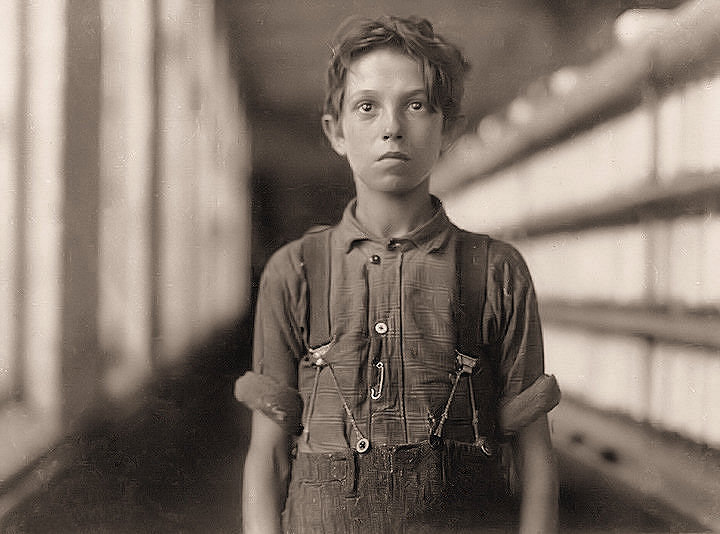
\includegraphics[width=3cm]{hine02}\par
  \raggedright
  \textit{Cover image: }
    The cover image shows Jo Bodeon, a back-roper in the mule room at 
    Chace Cotton Mill. Burlington, Vermont. This and other similar images 
    in this book were taken by Lewis W. Hine, in the period between 
    1908-1912. These images as well as social campaigns by many including 
    Hine, helped to formulate America's anti-child labour laws.
  \end{minipage}\par
  \vspace*{\baselineskip}
  \begin{minipage}[b]{0.9\textwidth}
  \RaggedRight
  \setlength{\parskip}{0.5\baselineskip}
  Copyright \copyright 2012  Dr Yiannis Lazarides\par
  Permission is granted to copy, distribute and\slash or modify this document 
  under the terms of the GNU Free Documentation License, version 1.2, with no 
  invariant sections, no front-cover texts, and no back-cover texts.\par
  A copy of the license is included in the appendix.\par
  This document is distributed in the hope that it will be useful, but without 
  any warranty; without even the implied warranty of merchantability or 
  fitness for a particular purpose.
  \end{minipage}
  \vspace*{2\baselineskip}
  \clearpage
}
%    \end{macrocode}
% \end{macro}
%
% \chapter{Table of Contents}
%
%	Most of the macros here re-write the LaTeX macros in a way that 
%	we can add appropriate hooks for styling. In writing this section
%	we had inspiration and used liberally code from Peter Wilson's 
%	\pkg{tocloft}., including the code for the image.
%
% \newcommand{\maxx}{120}       ^^A picture width
% \newcommand{\maxxm}{118}      ^^A \maxx - 2\
% \newcommand{\maxy}{55}        ^^A picture height
% \newcommand{\maxym}{53}       ^^A \maxy - 2
% \newcommand{\findent}{20}     ^^A indent
% \newcommand{\findentp}{22}    ^^A \findent + 2
% \newcommand{\fnumwidth}{10}   ^^A numwidth
% \newcommand{\ftocrmarg}{30}   ^^A \@tocrmarg
% \newcommand{\fpnumwidth}{20}  ^^A \@pnumwidth
% \newcommand{\fipn}{30}        ^^A \findent + \fnumwidth
% \newcommand{\frmarg}{90}      ^^A \maxx - \ftocrmarg
% \newcommand{\frnum}{100}      ^^A \maxx - \fpnumwidth
% \newcommand{\fyi}{10}         ^^A 1st y height
% \newcommand{\fyim}{8}         ^^A \fyi - 2
% \newcommand{\fyii}{20}        ^^A 2nd y height
% \newcommand{\fyiii}{25}       ^^A 3rd y height
% \newcommand{\fyiv}{30}        ^^A 4th y height
% \newcommand{\fyv}{40}         ^^A 5th y height
% \newcommand{\fyvp}{42}        ^^A \fyv + 2
% \newcommand{\flin}{4}         ^^A length of leader lines
% \newcommand{\frmargm}{89}     ^^A \frmarg (90) - a little bit
% 
% \providecommand{\bs}{\textbackslash}
% \begin{figure}
% \centering
% \setlength{\unitlength}{1mm}
% \begin{picture}(\maxx,\maxy)
%     ^^A side lines and linewidth
%   \put(0,0){\line(0,1){\maxy}}
%   \put(\maxx,0){\line(0,1){\maxy}}
%   \put(0,\maxy){\vector(1,0){\maxx}}
%   \put(2,\maxym){\makebox(0,0)[tl]{\texttt{\bs linewidth}}}
%     ^^A \@pnumwidth
%   \put(\maxx,\fyi){\vector(-1,0){\fpnumwidth}}
%   \put(\maxxm,\fyim){\makebox(0,0)[tr]{\texttt{\bs @pnumwidth}}}
%   \put(\frnum,\fyi){\line(0,1){\flin}}
%     ^^A \@tocrmarg
%   \put(\maxx,\fyv){\vector(-1,0){\ftocrmarg}}
%   \put(\maxxm,\fyvp){\makebox(0,0)[br]{\texttt{\bs @tocrmarg}}}
%   \put(\frmarg,\fyv){\line(0,-1){\flin}}
%     ^^A indent
%   \put(0,\fyv){\vector(1,0){\findent}}
%   \put(2,\fyvp){\makebox(0,0)[bl]{\textit{indent}}}
%   \put(\findent,\fyv){\line(0,-1){\flin}}
%     ^^A numwidth
%   \put(\findent,\fyv){\vector(1,0){\fnumwidth}}
%   \put(\findentp,\fyvp){\makebox(0,0)[bl]{\textit{numwidth}}}
%   \put(\fipn,\fyv){\line(0,-1){\flin}}
%     ^^A last title line
%   \put(\maxx,\fyii){\makebox(0,0)[br]{487}}
%   \put(\fipn,\fyii){title end}
%     ^^A second title line
%   \put(\fipn,\fyiii){continue\ldots}
%   \put(\frmarg,\fyiii){\makebox(0,0)[br]{\ldots title}}
%     ^^A first title line
%   \put(\findent,\fyiv){\textbf{3.5}}
%   \put(\fipn,\fyiv){Heading\ldots}
%   \put(\frmarg,\fyiv){\makebox(0,0)[br]{\ldots title}}
%     ^^A dotted leader
%   \multiput(\frmargm,\fyii)(-\flin,0){12}{.}
%   \multiput(\frmarg,\fyi)(-\flin,0){2}{\line(0,1){\flin}}
%   \put(\frmarg,\fyi){\vector(-1,0){\flin}}
%   \put(\frmarg,\fyi){\vector(1,0){0}}
%   \put(\frmarg,\fyim){\makebox(0,0)[tr]{\texttt{\bs @dotsep}}}
% 
% \end{picture}
% \setlength{\unitlength}{1pt}
% \caption{Layout of a ToC (LoF, LoT) entry} \label{fig:ltoc}
% \end{figure}
%
% \begin{macro}{\quit@cx}
% \begin{macro}{\if@haschapter@cx}
% We will be using either chapter or section type headings for the ToC, etc.,
% so we need to know which of these the document class supports.
%    \begin{macrocode}
\newcommand{\quit@cx}{}
\newif\if@haschapter@cx
%    \end{macrocode}
% \end{macro}
% \end{macro}
% \begin{macro}{\if@koma@cx}
% The \pkg{koma} classes have different defaults than the standard classes,
% so we need to know if a \pkg{koma} class has been loaded.
%    \begin{macrocode}
\newif\if@koma@cx  \@koma@cxfalse
\@ifclassloaded{scrartcl}{\@koma@cxtrue}{}
\@ifclassloaded{scrreprt}{\@koma@cxtrue}{}
\@ifclassloaded{scrbook}{\@koma@cxtrue}{}
%    \end{macrocode}
% \end{macro}
%
% \begin{macro}{\if@memoir@cx}
%    \begin{macrocode}
\newif\if@memoir@cx  \@memoir@cxfalse
\@ifclassloaded{memoir}{\@memoir@cxtrue}{}
%    \end{macrocode}
% \end{macro}
%
% Issue a warning if there are no recognised sectional divisions 
% and then skip the rest of the package code.
%    \begin{macrocode}
\@ifundefined{chapter}{%
  \@haschapter@cxfalse
  \@ifundefined{section}{%
    \PackageWarning{phd}%
      {I don't recognize any sectional divisions so I'll do nothing}
    \renewcommand{\quit@cx}{\endinput}
    }{\PackageInfo{phd}{The document has section divisions}}
  }{\@haschapter@cxtrue
    \PackageInfo{phd}{The document has chapter divisions}}
%    \end{macrocode}
% bailing out or continue.
%    \begin{macrocode}
\quit@cx
%    \end{macrocode}
%
% \begin{macro}{\settocpagestyle}
% \begin{macro}{\tocpagestyle@cx}
%	We define a user macro and to be used in keys
%   a pagestyle for the first page of the ToC.
%   The default is the |plain| pagestyle. CHECK THIS.
%    \begin{macrocode}
\newcommand{\settocpagestyle}[1]{%
  \def\tocpagestyle@cx{\thispagestyle{#1}}}
  \thispagestyle{plain}
%    \end{macrocode}
% \end{macro}
% \end{macro}
%
% \begin{macro}{\tocparskip@cx}
% The |\parskip| local to the ToC, etc., is set to the length |\tocparskip@cx|.
%
%    \begin{macrocode}
\newlength{\tocparskip@cx}
\setlength{\tocparskip@cx}{0pt}
%    \end{macrocode}
% \end{macro}
%
% 
% \begin{macro}{\tableofcontents}
% This is a parameterised version of the default |\tableofcontents| command.
% Each class has its own definition, but we have to cater for all classes
% in one definition, hence some of the checks. The definition is
% modified after all packages have been loaded.
%	Consider more checks here
%
%    \begin{macrocode}
\def\tocstart@cx{}
\def\tocfinish@cx{}
   \renewcommand{\tableofcontents}{%
    \tocstart@cx
%    \end{macrocode}
%     Ensure that any previous paragraph has been finished. 
%	 Within a group set
%     the local paragraphing style and typeset the title.
%    \begin{macrocode}
    \par
    \begingroup
      \parindent\z@ \parskip\tocparskip@cx
      \maketoctitle@cx
%    \end{macrocode}
%
% Finally, read the \file{.toc} file and finish up.
%    \begin{macrocode}
      \@starttoc{toc}%
    \endgroup
    \tocfinish@cx
}
%    \end{macrocode}
% \end{macro}
%
%    \begin{macrocode}
\newif\if@lowercase
\@lowercasetrue
\cxset{toc name/.code = \def\contentsname{#1},
       toc name before/.store in = \contentsnamebefore@cx,
       toc name after/.store in = \contentsnameafter@cx,
       toc name font-size/.store in = \contentsnamefontsize@cx,
       toc name font-weight/.store in = \contentsnamefontweight@cx,
       toc name font-family/.store in = \contentsnamefontfamily@cx,
       toc name font-shape/.store in = \contentsnamefontshape@cx,
       toc name color/.store in = \tocnamecolor@cx,
       toc name afterskip/.store in=\tocnameafterskip@cx,
       toc name align/.is choice,
       toc name align/center/.code=\def\startalign@cx{\center}\def\endalign@cx{\endcenter},
       toc name align/right/.code=\def\startalign@cx{\flushright}\def\endalign@cx{\endflushright},
       toc name align/left/.code=\def\startalign@cx{\@empty}\def\endalign@cx{\@empty},
       toc name align/none/.code=\def\startalign@cx{\@empty}\def\endalign@cx{\@empty},
       toc name case/.is choice,
       toc name case/lower/.code=\def\tocnamecase@cx{\@lowercasetrue
                             \if@lowercase\expandafter\MakeTextLowercase\fi},
       toc name case/upper/.code=\def\tocnamecase@cx{\@lowercasefalse
                             \if@lowercase\else\expandafter\MakeTextUppercase \fi},
      toc name case/none/.code=\def\tocnamecase@cx{\@empty},
    }

\cxset{toc name= CONTENTS,
       toc name before = ,
       toc name after =, 
       toc name color = teal,
       toc name font-weight=bold,
       toc name font-family=sffamily,
       toc name font-shape=upshape,
       toc name font-size=LARGE,
       toc name afterskip=10pt, %set as 40pt in LaTeX
       toc name after=\par,
       toc name align = left,
       toc name case= none,
}
%    \end{macrocode}

% \begin{macro}{\maketitle@cx}
%	\cs{maketitle@cx} is the typesetter for the heading that goes on top of the |ToC| page.
%	We cater for a few hooks, so the code is rather longish. At this point we can also 
%    divert to any custom design.
%    \begin{macrocode}
\newcommand{\maketoctitle@cx}{%
  \addpenalty\@secpenalty
  \if@haschapter@cx
    \vspace*{10pt}
    \pdfbookmark[0]{\contentsname}{toc}%EXPERIMENTAL
  \else
    \vspace{10pt}
  \fi
  %\@cftpagestyle
  {\interlinepenalty\@M
  {\contentsnamebefore@cx
     \setfont@cx{\contentsnamefontweight@cx}%
    {\contentsnamefontfamily@cx}{\contentsnamefontsize@cx}%
    {\contentsnamefontshape@cx}%
     \color{\tocnamecolor@cx}
     \startalign@cx \tocnamecase@cx
         \contentsname\endalign@cx}{\contentsnameafter@cx}
    
  \par\nobreak
  \vskip\tocnameafterskip@cx\relax
  \@afterheading}
 }
%    \end{macrocode}
% \end{macro}
%
% \begin{macro}{\setpnumwidth@cx}
% \begin{macro}{\setocmarg@cx}
%  Users commands for setting |\@pnumwidth| and |\@tocrmarg|.
%    \begin{macrocode}
\newcommand{\setpnumwidth@cx}[1]{\renewcommand{\@pnumwidth}{#1}}
\newcommand{\settocmarg@cx}[1]{\renewcommand{\@tocrmarg}{#1}}
\setpnumwidth@cx{25pt}
\settocmarg@cx{20pt}
%    \end{macrocode}
% \end{macro}
% \end{macro}
%
% \section{Styling the dot leaders}
%  	Here we will allow the user to either have dotfills and
%    be	able to specify the type and spacing of the dots.
%	We also provide a key to disable dotfills.
%
% \begin{macro}{\dot@cx}
% \begin{macro}{\dotfill@cx}
%   In the default |ToC|, a dotted line can be used to provide a leader between
%   a title and the page number. As Peter Wilson wrote and I found at my
%   distress the definition of the leader is buried
%   in the \cs{@dottedtocline} command. The 
%	\cs{dotfill@cx}\marg{sep}
%   command provides a parameterised version of the leader code, where
%   \marg{sep} is the seperation between the dots in mu units.
%   The symbol used for the `dots' in the leader is given by the 
%   value  of |\dot@cx|. 
% 
%    \begin{macrocode}
\newcommand{\dot@cx}{.}
\newcommand{\dotfill@cx}[1]{%
  \leaders\hbox{$\m@th\mkern #1 mu\hbox{\dot@cx}\mkern #1 mu$}\hfill}
%    \end{macrocode}
% \end{macro}
% \end{macro}
%
%    \begin{macrocode}
\def\nodotfill@cx{}
\cxset{toc dotfill/.is choice,
       toc dotfill/none/.code = \nodotfill@cx,
       toc dotfill symbol/.code= \renewcommand{\dot@cx}{#1},
       toc dotfill sep/.store in=\dotfillsep@cx,
}
\cxset{toc dotfill symbol=.,
       toc dotfill sep=4.5}
%    \end{macrocode}
%
% \begin{macro}{\parfillskip@CX}
% The |\l@kind| commands modify (locally) the value of |\parfillskip|.
% |\parfillskip@CX| is a copy of the default \texbook\ 
% |\parfillskip| definition.
%    \begin{macrocode}
\newcommand{\parfillskip@CX}{\parfillskip=0pt plus1fil}
%    \end{macrocode}
% \end{macro}
%
% \begin{macro}{\numberline}
% The purpose of the |\numberline{|\meta{secnum}|}| command is to typeset
% \meta{secnum} left justified in a box of width |\@tempdima|. I redefine
% it to add three additional parameters, namely |\tocnumberbefore@cx|, 
% |\@cftasnum| and |\@cftasnumb| 
% (see \file{ltsect.dtx} for the original
% definition).
%    \begin{macrocode}
\renewcommand{\numberline}[1]{% 
  \hb@xt@\@tempdima{\tocnumberbefore@cx #1\@cftasnum\hfil}\@cftasnumb}
%    \end{macrocode}
% \end{macro}
%
% \begin{macro}{\tocnumberbefore@cx}
% \begin{macro}{\@cftasnum}
% \begin{macro}{\@cftasnumb}
%
% Originally these were not defined but were |\let| to appropriate commands
% in the |\l@...| commands, but they
% have to be defined in case something unexpected 
% calls |\numberline|,
% for example through use of the \Lpack{float} package.\footnote{This bug WAS NOTED IN TOCLOF
% was discovered by Andrew Thurber when using the \Lpack{tocloft} and
% \Lpack{algorithm} packages together.}
%
%    \begin{macrocode}
\newcommand{\tocnumberbefore@cx}{[}
\newcommand{\@cftasnum}{}
\newcommand{\@cftasnumb}{}
%    \end{macrocode}
% \end{macro}
% \end{macro}
% \end{macro}
%
%
% \section{Styling the Toc Part}

% \begin{macro}{\l@part}
% \begin{macro}{\if@cftdopart}
%  |\l@part{|\meta{title}|}{|\meta{page}|}| typesets the ToC entry for
% a |part| heading. It is a parameterised copy of the default |\l@part|
% (see \file{classes.dtx} for the original definition and the code
%  below for |\l@subsection| for an explanation of most of this
%  code). By default, Parts
% (and Chapters) do not have dotted leaders. This package provides
% for all entries to have dotted leaders.
% In article class, Part level is 0 not -1 and hence the conditional below.
%	
%	We start by defining a number of keys and macros to store parameters.
%	An entry to the ToC consists always of a section number, the title and 
%	a page number. For each part there are different styling keys.
%
%	\begin{macro}{\tocpartindent@cx}	 
%    \begin{macrocode}
\cxset{toc part indent/.store in = \tocpartindent@cx,
       toc part numwidth/.store in = \tocpartnumwidth@cx,
       toc part font-size/.store in =\tocpartfontsize@cx,
       toc part before number/.store in = \tocpartbeforenumber@cx,
       toc part beforeskip/.store in = \tocpartbeforeskip@cx,
       toc part page font-size/.store in=\tocpartpagefontsize@cx,
       }
\cxset{toc part beforeskip = 2.25em \@plus\p@,
       toc part indent=0pt,
       toc part numwidth=0em,
       toc part font-size=\large\bfseries\sffamily,
       toc part before number=\kern1.5pt,
       toc part page font-size=\bfseries}
%    \end{macrocode}
% \end{macro}
%
%    \begin{macrocode}
\newif\if@dopart@cx
\newif\if@haspart@cx
\@ifundefined{part}{\@haspart@cxfalse}{\@haspart@cxtrue}
\if@haspart@cx


\renewcommand*{\l@part}[2]{%
  \@dopart@cxfalse
  \ifnum \c@tocdepth >-2\relax
    \if@haschapter@cx
      \@dopart@cxtrue
    \fi
    \ifnum \c@tocdepth >\m@ne
      \if@haschapter@cx\else
        \@dopart@cxtrue
      \fi
    \fi
  \fi
  \if@dopart@cx
    \if@haschapter@cx
      \addpenalty{-\@highpenalty}%
    \else
      \addpenalty\@secpenalty
    \fi
%    \end{macrocode}
%
%	We add vertical spacing before the section if
%	required.
%    \begin{macrocode}
    \addvspace{\tocpartbeforeskip@cx}%
    \begingroup
      {\leftskip \tocpartindent@cx\relax
       \rightskip \@tocrmarg % need to check this for conflics\@tocrmarg
       \parfillskip -\rightskip
       \parindent \tocpartindent@cx\relax
       \@afterindenttrue
       \interlinepenalty\@M
       \leavevmode    
       \@tempdima \tocpartnumwidth@cx\relax
%       \let\tocnumberbefore@cx \cftpartpresnum
%       \let\@cftasnum \cftpartaftersnum
%       \let\@cftasnumb \cftpartaftersnumb
       \advance\leftskip \@tempdima \null\nobreak\hskip -\leftskip
       %
       {\tocpartfontsize@cx 
       \tocpartbeforenumber@cx #1}%
       \cftpartfillnum{#2}}%
      \nobreak
      \if@haschapter@cx
        \global\@nobreaktrue
        \everypar{\global\@nobreakfalse\everypar{}}%
      \else
	  % removed compatibility stuff here don't care for earlier versions     
      \fi
    \endgroup
  \fi}
\fi
%    \end{macrocode}
% \end{macro}
% \end{macro}
%
% \begin{macro}{\cftbeforepartskip}
% \begin{macro}{\cftpartnumwidth}
% \begin{macro}{\cftpartfont}
% \begin{macro}{\cftpartpresnum}
% \begin{macro}{\cftpartaftersnum}
% \begin{macro}{\cftpartaftersnumb}
% \begin{macro}{\cftpartleader}
% \begin{macro}{\cftpartdotsep}
% \begin{macro}{\cftpartpagefont}
% \begin{macro}{\cftpartafterpnum}
% \begin{macro}{\cftpartindent}
% \begin{macro}{\cftpartfillnum}
%  These are the user commands to control the typesetting of Part entries.
%  They are initialised to give the standard appearance.
% \changes{v2.3a}{2002/10/03}{Deleted \cs{cftpartaftersnum} and \cs{cftpartaftersnumb}}
% \changes{v2.3b}{2003/01/20}{Reinstated \cs{cftpartaftersnum} and \cs{cftpartaftersnumb}}
%    \begin{macrocode}
\if@haspart@cx
%  \newlength{\cftbeforepartskip}
%    \setlength{\cftbeforepartskip}{2.25em \@plus\p@}
%  \newlength{\cftpartnumwidth}
%    \setlength{\cftpartnumwidth}{0em}
%  \newcommand{\cftpartfont}{\large\bfseries}
  \newcommand{\cftpartpresnum}{}
  \newcommand{\cftpartaftersnum}{}
  \newcommand{\cftpartaftersnumb}{}
%
% 
  \newcommand{\cftpartleader}{\large\bfseries\dotfill@cx{\cftpartdotsep}}
  \def\cftnodots{10000}
  \newcommand{\cftpartdotsep}{\cftnodots}
  \newcommand{\cftpartpagefont}{\large\bfseries}
  \newcommand{\cftpartafterpnum}{}
%  \newlength{\cftpartindent}
%    \setlength{\cftpartindent}{0em}
  \newcommand{\cftpartfillnum}[1]{%
    {\cftpartleader}%
    {\hb@xt@\@pnumwidth{\hss {%
       \tocpartpagefontsize@cx #1}}}\cftpartafterpnum\par}%
%    \end{macrocode}
% \Lpack{koma} classes use some different settings.
%   \begin{macrocode}
  \if@koma@cx
    %\setlength{\partnumwidth@cx}{2em}
    %\renewcommand{\cftpartfont}{\sectfont\large}
    %\renewcommand{\cftpartpagefont}{\sectfont\large}
  \fi
\fi

%    \end{macrocode}
% \end{macro}
% \end{macro}
% \end{macro}
% \end{macro}
% \end{macro}
% \end{macro}
% \end{macro}
% \end{macro}
% \end{macro}
% \end{macro}
% \end{macro}
% \end{macro}
%




% \begin{macro}{\beforetocchapterskip@cx}
% \begin{macro}{\cftchapindent}
% \begin{macro}{\cftchapnumwidth}
% \begin{macro}{\cftchapfont}
% \begin{macro}{\cftchappresnum}
% \begin{macro}{\cftchapaftersnum}
% \begin{macro}{\cftchapaftersnumb}
% \begin{macro}{\cftchapleader}
% \begin{macro}{\cftchapdotsep}
% \begin{macro}{\cftchappagefont}
% \begin{macro}{\cftchapafterpnum}
% \begin{macro}{\cftchapfillnum}
%  These are the user commands to control the typesetting of Chapter entries.
%  They are initialised to give the standard appearance.
%    \begin{macrocode}

\if@haschapter@cx
  \newlength{\beforetocchapterskip@cx}
    \setlength{\beforetocchapterskip@cx}{1.0em \@plus\p@}
  \newlength{\cftchapindent}
    \setlength{\cftchapindent}{0em}
  \newlength{\cftchapnumwidth}
    \setlength{\cftchapnumwidth}{1.5em}
  \newcommand{\cftchapfont}{\bfseries}
  \newcommand{\cftchappresnum}{}
  \newcommand{\cftchapaftersnum}{}
  \newcommand{\cftchapaftersnumb}{}
  \newcommand{\cftchapleader}{\bfseries\dotfill@cx{\cftchapdotsep}}
%    \end{macrocode}

%	The following code determines the spacing of he dots.
%    \begin{macrocode}
  \newcommand{\cftchapdotsep}{\chapterdotsep@cx} 
  \newcommand{\cftchappagefont}{\sffamily\bfseries\color{teal}}
  \newcommand{\cftchapafterpnum}{}
%
  \newcommand{\typesettocchapterpage@cx}[1]{%
    \hfill#1\par\addvspace{0.5\baselineskip}}
%    \end{macrocode}
%    \begin{macrocode}
% \Lpack{koma} classes have different chapter settings.
%    \begin{macrocode}
%  \if@cftkoma
%    \renewcommand{\cftchapfont}{\sectfont}
%  \fi
\fi

%    \end{macrocode}
% \end{macro}
% \end{macro}
% \end{macro}
% \end{macro}
% \end{macro}
% \end{macro}
% \end{macro}
% \end{macro}
% \end{macro}
% \end{macro}
% \end{macro}
% \end{macro}
% \begin{macro}{\l@chapter}
%  \cs{l@chapter}\marg{title}\marg{page} typesets the ToC entry for
% a |chapter| heading. It is a parameterised copy of the default |\l@chapter|
% (see \file{classes.dtx} for the original definition). This only applies
% to chaptered documents.
%    \begin{macrocode}

\newcommand{\chapternumberline}[3]{% 
  \hbox to 0pt{%
    \hspace*{-2cm}%
    \vbox to 0pt{\vspace*{.9cm}%
       \parbox[t]{2cm}{%
%         \ifx#3\empty\else
%            \includegraphics[width=1.5cm]{#3}%
%         \fi
         }}}

  \hspace*{-2cm}\parbox[t]{25pt}{#1}%
  \parbox[t]{.6\linewidth}{{\RaggedRight#2}\par}%
}


\cxset{toc chapter beforeskip/.store in=\beforetocchapterskip@cx,
       toc chapter indent/.store in = \tocchapterindent@cx,
       toc chapter dotsep/.store in = \chapterdotsep@cx,
       toc chapter no dots/.code=\def\chapterdotsep@cx{10000},
       toc chapter numberwidth/.store in = \tocchapternumberwidth@cx,
       toc chapter font/.store in=\tocchapterfont@cx}


\cxset{toc chapter beforeskip =0pt,
       toc chapter indent= 0pt,
       toc chapter dotsep=4.5,
       toc chapter no dots,
       toc chapter numberwidth=0pt,
       toc chapter font= \bfseries\sffamily\large\color{teal}}

\if@haschapter@cx
\renewcommand*{\l@chapter}[2]{%
  \ifnum \c@tocdepth >\m@ne
    \addpenalty{-\@highpenalty}%
    \vskip \beforetocchapterskip@cx\relax
    {%\leftskip\tocchapterindent@cx\relax
     %\rightskip \@tocrmarg
     %\parfillskip -\rightskip
     \parindent \tocchapterindent@cx\relax\@afterindenttrue
     %\interlinepenalty\@M
     \leavevmode
     %\@tempdima \tocchapternumberwidth@cx\relax
     %\let\tocnumberbefore@cx \cftchappresnum
     %\let\@cftasnum \cftchapaftersnum
     %\let\@cftasnumb \cftchapaftersnumb
     %\advance\leftskip \@tempdima \null\nobreak\hskip -\leftskip
     {\tocchapterfont@cx #1}\nobreak
     \typesettocchapterpage@cx{#2}}%
  \fi}%
\fi
%    \end{macrocode}
% \end{macro}
%
% \section{ToC section hooks}
%
%  |\l@section{|\meta{title}|}{|\meta{page}|}| typesets the ToC entry for
% a |section| heading. It is a parameterised copy of the default |\l@section|
% (see \file{classes.dtx} for the original definition). 
% 	We start by defining all our parameters and variables.
%
%    \begin{macrocode}
\renewcommand{\numberline}[1]{% 
  \hb@xt@\@tempdima{#1\hfil}}
\cxset{toc section beforeskip/.store in=\tocsectionbeforeskip@cx,
       toc section indent/.store in=\tocsectionindent@cx,
%      fonts for title &num
       toc section font-size/.store in=\tocsectionfontsize@cx, 
       toc section font-family/.store in=\tocsectionfontfamily@cx, 
       toc section font-shape/.store in=\tocsectionfontshape@cx, 
       toc section font-weight/.store in=\tocsectionfontweight@cx, 
       toc section color/.store in=\tocsectioncolor@cx,
       toc section numwidth/.store in=\tocsectionnumwidth@cx,
%	  fonts etc for page number
       toc section page font-size/.store in=\tocsectionpagefontsize@cx,
       toc section page font-family/.store in=\tocsectionpagefontfamily@cx,
       toc section page font-shape/.store in=\tocsectionpagefontshape@cx,
       toc section page font-weight/.store in=\tocsectionpagefonteight@cx,
       toc section page color/.store in=\tocsectionpagecolor@cx,
%      leaders
	   toc section dotsep/.store in = \tocsecdotsep@cx,
%      before and after page number
       toc section page before/.store in=\tocsectionpagebefore@cx,
       toc section page after/.store in=\tocsectionpageafter@cx,
}

\cxset{%
       toc section beforeskip=\z@ \@plus.2\p@,
       toc section indent=0em,
       toc section font-family= sffamily,
       toc section font-weight = mdseries,
       toc section font-shape = upshape,
       toc section color= teal,
       toc section font-size=,
       toc section numwidth = 2.8em,
       toc section page font-size=,
       toc section page font-shape= upshape,  
       toc section page font-weight=, 
       toc section page font-family= sffamily,
       toc section page color = teal, 
       toc section page before =,% \{,
       toc section page after =,% \},
       toc section dotsep = 2.7,
}
%    \end{macrocode}
%
%  
% \begin{macro}{\tocsectionpagefont@cx}
%    For convenience we define font setting commands for
%    the page number. We use \cs{setfont@cx}, which we have
%	defined earlier.
%  
%    \begin{macrocode}
\newcommand\tocsectionpagefont@cx{%
	\setfont@cx{\tocsectionpagefonteight@cx}%
       {\tocsectionpagefontfamily@cx}{\tocsectionpagefontsize@cx}%
       {\tocsectionpagefontshape@cx}\color{\tocsectionpagecolor@cx}
}%
%    \end{macrocode}
% \end{macro}
%
% \begin{macro}{\l@section} 
% 	This macro is called when the \cs{tableofcontents}
%	is read from the |.toc| file and it typesets
%	the title and the page number. Note this is also
% 
%    \#1 section title
%    \#2 page number
%      
%    \begin{macrocode}
\renewcommand*{\l@section}[2]{%
  \ifnum \c@tocdepth >\z@
    \if@haschapter@cx
      \vskip \tocsectionbeforeskip@cx
    \else
      \addpenalty \@secpenalty
      \addvspace{\tocsectionbeforeskip@cx}%
    \fi
    {\leftskip \tocsectionindent@cx\relax
     \rightskip \@tocrmarg
     \parfillskip -\rightskip
     \parindent \tocsectionindent@cx\relax\@afterindenttrue
     \interlinepenalty\@M
     \leavevmode
     \@tempdima \tocsectionnumwidth@cx\relax
     \let\tocnumberbefore@cx \cftsecpresnum
     \let\@cftasnum \cftsecaftersnum
     \let\@cftasnumb \cftsecaftersnumb
     \advance\leftskip \@tempdima \null\nobreak\hskip -\leftskip
%    \end{macrocode}
%
%	We are now ready to print out the toc section title,
%	we set the font information then typeset the title.
%	The dot leaders are typeset by calling the 
%	macro \cs{sectionfillnum}
%
%    \begin{macrocode}
     {%
      \setfont@cx{\tocsectionfontweight@cx}%
        {\tocsectionfontfamily@cx}{\tocsectionfontsize@cx}%
        {\tocsectionfontshape@cx}%
        \color{\tocsectioncolor@cx}%
      #1}\nobreak
%    \end{macrocode}
%	We are now ready to typeset the leaders and the page number. 
%    We then pass \#2 to the \cs{tocsectionfillnum} which 
%	does the typesetting.
%    \begin{macrocode}
      \tocsectionfillnum@cx{#2}}%
  \fi}
%    \end{macrocode}
% \end{macro}
%
%    These are the user commands to control the typesetting 
%	 of Section entries.
%    They are initialised to give the standard appearance.
%	 These are hooks to \cs{numberline}.
%    \begin{macrocode}
\newcommand{\cftsecpresnum}{}
\newcommand{\cftsecaftersnum}{}
\newcommand{\cftsecaftersnumb}{}
\newcommand{\tocsectionleader@cx}  {\normalfont\dotfill@cx{\tocsecdotsep@cx}}
%\newcommand{\cftsecdotsep}{\cftdotsep}
%    \end{macrocode}
%    We can now define the command \cmd{\tocsectionfillnum@cx}. 
%    will print the 
%	leaders if any and the page number \#1. 
%    \begin{macrocode}
\newcommand{\tocsectionfillnum@cx}[1]{%
  {\tocsectionleader@cx}\nobreak
  \hb@xt@\@pnumwidth{\hfil\tocsectionpagefont@cx
   \tocsectionpagebefore@cx #1}%
   \tocsectionpageafter@cx\par}%
%    \end{macrocode}
%
%
% \section{Toc subsection styling}
% \begin{macro}{\l@subsection}
%  |\l@subsection{|\meta{title}|}{|\meta{page}|}| typesets the ToC entry for
% a |section| heading. It is a parameterised copy of the default |\l@section|
% (see \file{classes.dtx} for the original definition). 
% 	We start by defining all our parameters and variables.
%
%    \begin{macrocode}
\newif\if@lowercasesubsection
\cxset{toc subsection beforeskip/.store in=\tocsubsectionbeforeskip@cx,
       toc subsection indent/.store in=\tocsubsectionindent@cx,
%      fonts for title &num
       toc subsection font-size/.store in=\tocsubsectionfontsize@cx, 
       toc subsection font-family/.store in=\tocsubsectionfontfamily@cx, 
       toc subsection font-shape/.store in=\tocsubsectionfontshape@cx, 
       toc subsection font-weight/.store in=\tocsubsectionfontweight@cx, 
       toc subsection color/.store in=\tocsubsectioncolor@cx,
toc subsection case/.is choice,
       toc subsection case/lower/.code=\def\tocsubsectioncase@cx{\@lowercasesubsectiontrue
                             \if@lowercasesubsection\expandafter\MakeTextLowercase\fi},
       toc subsection case/upper/.code=\def\tocsubsectioncase@cx{\@lowercasesubsectionfalse
                    \if@lowercasesubsection\else\expandafter\MakeTextUppercase \fi},
       toc subsection case/none/.code=\def\tocsubsectioncase@cx{\@empty},
       toc subsection numwidth/.store in=\tocsubsectionnumwidth@cx,
%	  fonts etc for page number
       toc subsection page font-size/.store in=\tocsubsectionpagefontsize@cx,
       toc subsection page font-family/.store in=\tocsubsectionpagefontfamily@cx,
       toc subsection page font-shape/.store in=\tocsubsectionpagefontshape@cx,
       toc subsection page font-weight/.store in=\tocsubsectionpagefonteight@cx,
       toc subsection page color/.store in=\tocsubsectionpagecolor@cx,
%      leaders
	   toc subsection dotsep/.store in = \tocsubsecdotsep@cx,
%      before and after page number
       toc subsection page before/.store in=\tocsubsectionpagebefore@cx,
       toc subsection page after/.store in=\tocsubsectionpageafter@cx,
}

\cxset{toc subsection beforeskip=\z@ \@plus.2\p@,
       toc subsection indent=0em,
       toc subsection font-family= sffamily,
       toc subsection font-weight = mdseries,
       toc subsection font-shape = upshape,
       toc subsection color= teal,
       toc subsection font-size=,
       toc subsection case = none,
       toc subsection numwidth = 2.8em,
       toc subsection page font-size=,
       toc subsection page font-shape= upshape,  
       toc subsection page font-weight=, 
       toc subsection page font-family= sffamily,
       toc subsection page color = teal, 
       toc subsection page before =,% \{,
       toc subsection page after =,% \},
       toc subsection dotsep = 2.7,
}
%    \end{macrocode}
%
%    For convenience we define font setting commands for
%    the page number. We use \cs{setfont@cx}, which we have
%	defined earlier.
%    
%    \begin{macrocode}
\newcommand\tocsubsectionpagefont@cx{%
	\setfont@cx{\tocsubsectionpagefonteight@cx}%
       {\tocsubsectionpagefontfamily@cx}{\tocsubsectionpagefontsize@cx}%
       {\tocsubsectionpagefontshape@cx}\color{\tocsubsectionpagecolor@cx}
}%
        

\renewcommand*{\l@subsection}[2]{%
  \ifnum \c@tocdepth >\z@
    \if@haschapter@cx
      \vskip \tocsubsectionbeforeskip@cx
    \else
      \addpenalty \@secpenalty
      \addvspace{\tocsubsectionbeforeskip@cx}%
    \fi
    {\leftskip \tocsubsectionindent@cx\relax
     \rightskip \@tocrmarg
     \parfillskip -\rightskip
     \parindent \tocsubsectionindent@cx\relax\@afterindenttrue
     \interlinepenalty\@M
     \leavevmode
     \@tempdima \tocsubsectionnumwidth@cx\relax
     \let\tocnumberbefore@cx \cftsecpresnum
     \let\@cftasnum \cftsecaftersnum
     \let\@cftasnumb \cftsecaftersnumb
     \advance\leftskip \@tempdima \null\nobreak\hskip -\leftskip
%    \end{macrocode}
%
%	We are now ready to print out the toc subsection title,
%	we set the font information then typeset the title.
%	The dot leaders are typeset by calling the macro \cs{sectionfillnum}
%
%    \begin{macrocode}
     {%
      \setfont@cx{\tocsubsectionfontweight@cx}%
        {\tocsubsectionfontfamily@cx}{\tocsubsectionfontsize@cx}%
        {\tocsubsectionfontshape@cx}%
        \color{\tocsubsectioncolor@cx}%
      \tocsubsectioncase@cx#1}\nobreak
%    \end{macrocode}
%	We are now ready to typeset the leaders and the page number. 
%    We then pass \#2 to the \cs{tocsectionfillnum} which 
%	does the typesetting.
%    \begin{macrocode}
      \tocsubsectionfillnum{#2}}%
  \fi}
%    \end{macrocode}
% \end{macro}
%
%    These are the user commands to control the typesetting of Section entries.
%    They are initialised to give the standard appearance.
%    \begin{macrocode}
% hooks to |\numberline|
\renewcommand{\cftsecpresnum}{.}
\renewcommand{\cftsecaftersnum}{..}
\renewcommand{\cftsecaftersnumb}{...}
\newcommand{\tocsubsectionleader}{\normalfont\dotfill@cx{\tocsubsecdotsep@cx}}
%\newcommand{\cftsecdotsep}{\cftdotsep}
%    \end{macrocode}
%    We can now define the command \cmd{\tocsectionfillnum}. It will print the 
%	leaders if any and the page number \#1. TODO IS par necessary??
%    \begin{macrocode}
\newcommand{\tocsubsectionfillnum}[1]{%
  {\tocsubsectionleader}\nobreak
  \hb@xt@\@pnumwidth{\hfil\tocsubsectionpagefont@cx
   \tocsubsectionpagebefore@cx #1}%
   \tocsubsectionpageafter@cx\par}%
%    \end{macrocode}
%
% \section{Toc subsubsection styling}
% \begin{macro}{\l@subsubsection}
%  |\l@subsubsection{|\meta{title}|}{|\meta{page}|}| typesets the ToC entry for
% a |subsubsection| heading. It is a parameterised copy of the default |\l@subsubsection|
%	We start by defining all our parameters and variables.
%
%    \begin{macrocode}
\newif\if@lowercasesubsubsection
\cxset{toc subsubsection beforeskip/.store in=\tocsubsubsectionbeforeskip@cx,
       toc subsubsection indent/.store in=\tocsubsubsectionindent@cx,
%      fonts for title &num
       toc subsubsection font-size/.store in=\tocsubsubsectionfontsize@cx, 
       toc subsubsection font-family/.store in=\tocsubsubsectionfontfamily@cx, 
       toc subsubsection font-shape/.store in=\tocsubsubsectionfontshape@cx, 
       toc subsubsection font-weight/.store in=\tocsubsubsectionfontweight@cx, 
       toc subsubsection color/.store in=\tocsubsubsectioncolor@cx,
toc subsubsection case/.is choice,
       toc subsubsection case/lower/.code=\def\tocsubsubsectioncase@cx{\@lowercasesubsubsectiontrue
                             \if@lowercasesubsubsection\expandafter\MakeTextLowercase\fi},
       toc subsubsection case/upper/.code=\def\tocsubsubsectioncase@cx{\@lowercasesubsubsectionfalse
                    \if@lowercasesubsubsection\else\expandafter\MakeTextUppercase \fi},
       toc subsubsection case/none/.code=\def\tocsubsubsectioncase@cx{\@empty},
       toc subsubsection numwidth/.store in=\tocsubsubsectionnumwidth@cx,
%	  fonts etc for page number
       toc subsubsection page font-size/.store in=\tocsubsubsectionpagefontsize@cx,
       toc subsubsection page font-family/.store in=\tocsubsubsectionpagefontfamily@cx,
       toc subsubsection page font-shape/.store in=\tocsubsubsectionpagefontshape@cx,
       toc subsubsection page font-weight/.store in=\tocsubsubsectionpagefonteight@cx,
       toc subsubsection page color/.store in=\tocsubsubsectionpagecolor@cx,
%      leaders
	   toc subsubsection dotsep/.store in = \tocsubsubsecdotsep@cx,
%      before and after page number
       toc subsubsection page before/.store in=\tocsubsubsectionpagebefore@cx,
       toc subsubsection page after/.store in=\tocsubsubsectionpageafter@cx,
}

\cxset{toc subsubsection beforeskip=\z@ \@plus.2\p@,
       toc subsubsection indent=0em,
       toc subsubsection font-family= sffamily,
       toc subsubsection font-weight = mdseries,
       toc subsubsection font-shape = upshape,
       toc subsubsection color= teal,
       toc subsubsection font-size=,
       toc subsubsection case = none,
       toc subsubsection numwidth = 2.8em,
       toc subsubsection page font-size=,
       toc subsubsection page font-shape= upshape,  
       toc subsubsection page font-weight=, 
       toc subsubsection page font-family= sffamily,
       toc subsubsection page color = teal, 
       toc subsubsection page before =,% \{,
       toc subsubsection page after =,% \},
       toc subsubsection dotsep = 2.7,
}
%    \end{macrocode}
%
%    For convenience we define font setting commands for
%    the page number. We use \cs{setfont@cx}, which we have
%	defined earlier.
%    
%    \begin{macrocode}
\newcommand\tocsubsubsectionpagefont@cx{%
	\setfont@cx{\tocsubsubsectionpagefonteight@cx}%
       {\tocsubsubsectionpagefontfamily@cx}{\tocsubsubsectionpagefontsize@cx}%
       {\tocsubsubsectionpagefontshape@cx}\color{\tocsubsubsectionpagecolor@cx}
}%
        

\renewcommand*{\l@subsubsection}[2]{%
  \ifnum \c@tocdepth >\z@
    \if@haschapter@cx
      \vskip \tocsubsubsectionbeforeskip@cx
    \else
      \addpenalty \@secpenalty
      \addvspace{\tocsubsubsectionbeforeskip@cx}%
    \fi
    {\leftskip \tocsubsubsectionindent@cx\relax
     \rightskip \@tocrmarg
     \parfillskip -\rightskip
     \parindent \tocsubsubsectionindent@cx\relax\@afterindenttrue
     \interlinepenalty\@M
     \leavevmode
     \@tempdima \tocsubsubsectionnumwidth@cx\relax
     \let\tocnumberbefore@cx \cftsecpresnum
     \let\@cftasnum \cftsecaftersnum
     \let\@cftasnumb \cftsecaftersnumb
     \advance\leftskip \@tempdima \null\nobreak\hskip -\leftskip
%    \end{macrocode}
%
%	We are now ready to print out the toc subsection title,
%	we set the font information then typeset the title.
%	The dot leaders are typeset by calling the macro \cs{sectionfillnum}
%
%    \begin{macrocode}
     {%
      \setfont@cx{\tocsubsubsectionfontweight@cx}%
        {\tocsubsubsectionfontfamily@cx}{\tocsubsubsectionfontsize@cx}%
        {\tocsubsubsectionfontshape@cx}%
        \color{\tocsubsubsectioncolor@cx}%
      \tocsubsubsectioncase@cx#1}\nobreak
%    \end{macrocode}
%	We are now ready to typeset the leaders and the page number. 
%    We then pass \#2 to the \cs{tocsectionfillnum} which 
%	does the typesetting.
%    \begin{macrocode}
      \tocsubsubsectionfillnum{#2}}%
  \fi}
%    \end{macrocode}
% \end{macro}
%
%    These are the user commands to control the typesetting of Section entries.
%    They are initialised to give the standard appearance.
%    \begin{macrocode}
% hooks to |\numberline|
\renewcommand{\cftsecpresnum}{.}
\renewcommand{\cftsecaftersnum}{..}
\renewcommand{\cftsecaftersnumb}{...}
\newcommand{\tocsubsubsectionleader}{\normalfont\dotfill@cx{\tocsubsubsecdotsep@cx}}
%\newcommand{\cftsecdotsep}{\cftdotsep}
%    \end{macrocode}
%    We can now define the command \cmd{\tocsectionfillnum}. It will print the 
%	leaders if any and the page number \#1. TODO IS par necessary??
%    \begin{macrocode}
\newcommand{\tocsubsubsectionfillnum}[1]{%
  {\tocsubsubsectionleader}\nobreak
  \hb@xt@\@pnumwidth{\hfil\tocsubsubsectionpagefont@cx
   \tocsubsubsectionpagebefore@cx #1}%
   \tocsubsubsectionpageafter@cx\par}%
%    \end{macrocode}
%
% \section{Toc paragraph styling}
% \begin{macro}{\l@paragraph}
%  |\l@subsubsection{|\meta{title}|}{|\meta{page}|}| typesets the ToC entry for
% a |subsubsection| heading. It is a parameterised copy of the default |\l@subsubsection|
%	We start by defining all our parameters and variables.
%
%    \begin{macrocode}
\newif\if@lowercaseparagraph
\cxset{toc paragraph beforeskip/.store in=\tocparagraphbeforeskip@cx,
       toc paragraph indent/.store in=\tocparagraphindent@cx,
%      fonts for title &num
       toc paragraph font-size/.store in=\tocparagraphfontsize@cx, 
       toc paragraph font-family/.store in=\tocparagraphfontfamily@cx, 
       toc paragraph font-shape/.store in=\tocparagraphfontshape@cx, 
       toc paragraph font-weight/.store in=\tocparagraphfontweight@cx, 
       toc paragraph color/.store in=\tocparagraphcolor@cx,
toc paragraph case/.is choice,
       toc paragraph case/lower/.code=\def\tocparagraphcase@cx{\@lowercaseparagraphtrue
                             \if@lowercaseparagraph\expandafter\MakeTextLowercase\fi},
       toc paragraph case/upper/.code=\def\tocparagraphcase@cx{\@lowercaseparagraphfalse
                    \if@lowercaseparagraph\else\expandafter\MakeTextUppercase \fi},
       toc paragraph case/none/.code=\def\tocparagraphcase@cx{\@empty},
       toc paragraph numwidth/.store in=\tocparagraphnumwidth@cx,
%	  fonts etc for page number
       toc paragraph page font-size/.store in=\tocparagraphpagefontsize@cx,
       toc paragraph page font-family/.store in=\tocparagraphpagefontfamily@cx,
       toc paragraph page font-shape/.store in=\tocparagraphpagefontshape@cx,
       toc paragraph page font-weight/.store in=\tocparagraphpagefonteight@cx,
       toc paragraph page color/.store in=\tocparagraphpagecolor@cx,
%      leaders
	   toc paragraph dotsep/.store in = \tocparagraphdotsep@cx,
%      before and after page number
       toc paragraph page before/.store in=\tocparagraphpagebefore@cx,
       toc paragraph page after/.store in=\tocparagraphpageafter@cx,
}

\cxset{toc paragraph beforeskip=\z@ \@plus.2\p@,
       toc paragraph indent=0em,
       toc paragraph font-family= sffamily,
       toc paragraph font-weight = mdseries,
       toc paragraph font-shape = upshape,
       toc paragraph color= teal,
       toc paragraph font-size=,
       toc paragraph case = none,
       toc paragraph numwidth = 2.8em,
       toc paragraph page font-size=,
       toc paragraph page font-shape= upshape,  
       toc paragraph page font-weight=, 
       toc paragraph page font-family= sffamily,
       toc paragraph page color = teal, 
       toc paragraph page before =,% \{,
       toc paragraph page after =,% \},
       toc paragraph dotsep = 2.7,
}
%    \end{macrocode}
%
% \cxset{subsubsection numbering=none,
%        subsubsection numbering prefix=,
%        subsubsection indent =0pt,
%        paragraph numbering=none,
%        paragraph indent=0pt,
%        paragraph beforeskip= 0pt,
%        subparagraph beforeskip=0pt,
%        subparagraph numbering=none}
%   \renewsubsection
%   \renewparagraph
%   \renewsubparagraph
%   \renewsubsubsection
%	\subsection{Default paragraph style}
%   \subsubsection{With a subsubsection}
%
%
%	\paragraph{Test paragraph} This is a test.
%
%    For convenience we define font setting commands for
%    the page number. We use \cs{setfont@cx}, which we have
%	defined earlier.
%    
%    \begin{macrocode}
\newcommand\tocparagraphpagefont@cx{%
	\setfont@cx{\tocparagraphpagefonteight@cx}%
       {\tocparagraphpagefontfamily@cx}{\tocparagraphpagefontsize@cx}%
       {\tocparagraphpagefontshape@cx}\color{\tocparagraphpagecolor@cx}
}%
        

\renewcommand*{\l@paragraph}[2]{%
  \ifnum \c@tocdepth >\z@
    \if@haschapter@cx
      \vskip \tocparagraphbeforeskip@cx
    \else
      \addpenalty \@secpenalty
      \addvspace{\tocparagraphbeforeskip@cx}%
    \fi
    {\leftskip \tocparagraphindent@cx\relax
     \rightskip \@tocrmarg
     \parfillskip -\rightskip
     \parindent \tocparagraphindent@cx\relax\@afterindenttrue
     \interlinepenalty\@M
     \leavevmode
     \@tempdima \tocparagraphnumwidth@cx\relax
     \let\tocnumberbefore@cx \cftsecpresnum
     \let\@cftasnum \cftsecaftersnum
     \let\@cftasnumb \cftsecaftersnumb
     \advance\leftskip \@tempdima \null\nobreak\hskip -\leftskip
%    \end{macrocode}
%
%	We are now ready to print out the toc subsection title,
%	we set the font information then typeset the title.
%	The dot leaders are typeset by calling the macro \cs{sectionfillnum}
%
%    \begin{macrocode}
     {%
      \setfont@cx{\tocparagraphfontweight@cx}%
        {\tocparagraphfontfamily@cx}{\tocparagraphfontsize@cx}%
        {\tocparagraphfontshape@cx}%
        \color{\tocparagraphcolor@cx}%
      \tocparagraphcase@cx#1}\nobreak
%    \end{macrocode}
%	We are now ready to typeset the leaders and the page number. 
%    We then pass \#2 to the \cs{tocsectionfillnum} which 
%	does the typesetting.
%    \begin{macrocode}
      \tocparagraphfillnum{#2}}%
  \fi}
%    \end{macrocode}
% \end{macro}
%
%    These are the user commands to control the typesetting of Section entries.
%    They are initialised to give the standard appearance.
%    \begin{macrocode}
% hooks to |\numberline|
\renewcommand{\cftsecpresnum}{.}
\renewcommand{\cftsecaftersnum}{..}
\renewcommand{\cftsecaftersnumb}{...}
\newcommand{\tocparagraphleader}{\normalfont\dotfill@cx{\tocparagraphdotsep@cx}}
%\newcommand{\cftsecdotsep}{\cftdotsep}
%    \end{macrocode}
%    We can now define the command \cmd{\tocsectionfillnum}. It will print the 
%	leaders if any and the page number \#1. TODO IS par necessary??
%    \begin{macrocode}
\newcommand{\tocparagraphfillnum}[1]{%
  {\tocparagraphleader}\nobreak
  \hb@xt@\@pnumwidth{\hfil\tocparagraphpagefont@cx
   \tocparagraphpagebefore@cx #1}%
   \tocparagraphpageafter@cx\par}%
%    \end{macrocode}
%
% \chapter{Handling Images}
% \precis{Commands for laying out complex pages composed primarily of images.}

% \section{creating Image Page Styles}
%
% We now develop a method to produce variable environments
% that can include images in a page. We start using designs
% that incorporate two columns, as shown on 
% Page~\pageref{krollcode}.
%
% \begin{macro}{\miniwidthi}
% \begin{macro}{\miniwidthii}
% \begin{macro}{\sepmainhorizontal}
%    \begin{macrocode}
\global\newlength{\miniwidthi}
\global\newlength{\miniwidthii}
\global\newlength{\sepmainhorizontal}
\def\tinyskip{\vskip2pt}
%    \end{macrocode}
% \end{macro}
% \end{macro}
% \end{macro}
%    \begin{macrocode}
\newenvironment{leftcolumn}{}{}
\newenvironment{rightcolumn}{}{}

\newlength\offsetfromright
\setlength\offsetfromright{0em}
%    \end{macrocode}
%
% \begin{macro}{\onelinecaption} The oneline caption
% is the description that goes underneath images that
% unlike figures, they are not descibed in the text.
%    \begin{macrocode}
\newcommand\onelinecaption[2][]{%
    \setlength\offsetfromright{0em}%
    \bgroup%
        \vskip0pt plus1pt minus1pt %
        \reset@font
        \sffamily
        \bfseries%
        \footnotesize%
        \hfill\hfill#2\hbox to \offsetfromright{}%
     \egroup%
}
%    \end{macrocode}
% \end{macro}
% 
% \begin{macro}{\onelineheader} This macro takes one parameter
%   and styles the main header.
%    \begin{macrocode}
\long\def\onelineheader#1{%
 \vspace{1.5\baselineskip}%
 {\sffamily{\bgroup\LARGE\bf \mbox{#1}\egroup}%
 \vspace{0.5\baselineskip}}%
}
%    \end{macrocode}
% \end{macro}
%    \begin{macrocode}
\newcommand\byline[2][]{\small{\bfseries#1}#2}
 \newcommand\MainHeader[1]{{\leavevmode\par\centering \textrm{\fontsize{50pt}{65pt}\selectfont #1}\par\vspace{1cm}}}
 \newcommand\MainHeadera[1]{{\leavevmode\par\centering \textrm{\fontsize{30pt}{42pt}\selectfont #1}\par\vspace{1cm}}}
%    \end{macrocode}
%
%    \begin{macrocode}
\def\aheader#1{\footnotesize \textbf{SELF-PORTRAIT}#1}
 \renewenvironment{leftcolumn}[1]{%
        \begin{minipage}[b]{\miniwidthi} #1}{\end{minipage} \hspace{\sepmainhorizontal}}%
    \renewenvironment{rightcolumn}[1]{%
        \begin{minipage}[b]{\miniwidthii} #1}{\end{minipage}}%
\def\starttemplate#1{%
  %% we now calculate some of the parameters
%% required
    \setlength\miniwidthi{0.3\textwidth}%
    \setlength\miniwidthii{0.67\textwidth}%
    \setlength\sepmainhorizontal{0.03\textwidth}%
   %
   %
%% Create environments for convenience
   %% Create right column environment
}
 \def\stoptemplate{}
%
%% Defining kroll style
  %% We need to find a way to define the templates
%% We will assume that images have been saved in a database
%% image@file
%% image@caption
%% this is a must to avoid long typing and keep the environments
%% short
\fboxsep=0pt
\fboxrule=1pt

\define@key{img}{width}[1cm]{\def\img@width{#1}}
\define@key{img}{height}{\def\img@height{#1}}
\define@key{img}{offsetx}{\def\img@offsetx{#1}}
\define@key{img}{offsety}{\def\img@offsety{#1}}
\define@key{img}{border}{\def\img@border{#1}}
\define@key{img}{padding}{\def\img@padding{#1}}
\define@key{img}{style}{\def\img@style{#1}}
\define@key{img}{bottommargin}{\def\img@bottommargin{#1}}
\define@key{img}{keepaspectratio}{\def\img@keepaspectratio{keepaspectratio}}
\define@key{imgpg}{pagestyle}{\def\imgpg@pagestyle{#1}}
%% Set defaults for all keys
\setkeys{img}{offsetx=1sp, offsety=0pt,width=3cm, keepaspectratio=keepaspectratio,
                      border=0pt, padding=0pt,bottommargin=0pt}
%% Create the command graphic
\newlength\tempa

%% We create a new command to place images 
\newcommand\putimage[2][0pt]{%
%% Set the keys
\setkeys{img}{#1}%
\setlength\fboxrule\img@border%
\setlength\fboxsep\img@padding%
\ifdim\img@offsety=0pt% 
\else%
\vspace*{\img@offsety}%
\fi%
\hskip\img@offsetx%
\setlength{\tempa}{\img@width}
\fboxsep=1pt
\def\setcaption{\captionof{figure}{This is the caption for the figure\lorem}}%
\begin{minipage}{\textwidth}%
\fbox{\includegraphics[width=\textwidth]{#2}}%
\end{minipage}
}%\vspace*{\img@bottommargin}}%
%    \end{macrocode}
%
% 
% \clearpage
% 
% \newgeometry{top=0.5cm, bottom=1cm, left=1cm, right=1cm,
%               marginparsep=0cm, marginpar=0pt}
% 
% \clearpage 
% \newpage

% \hrule
% \mbox{}
%    
% \label{krollcode}
% \renewenvironment{leftcolumn}{%
%   \minipage[b]{.3\textwidth}%
%  }{\endminipage}\hspace*{0cm}%
% 
% \starttemplate{kroll}%
% \vspace*{-.8cm}
% \hspace*{-1cm}\begin{leftcolumn}%
%   \MainHeader{Leon\\[15pt] Kroll}
%   \putimage[width=0.5\linewidth]{krollportrait}\par
%   \aheader{shows Kroll at 59. Says he. ``Painting is 
%             fascinating'' even when motif my own mug.}
% \end{leftcolumn}%
% \begin{minipage}[b]{0.8\textwidth}%
%   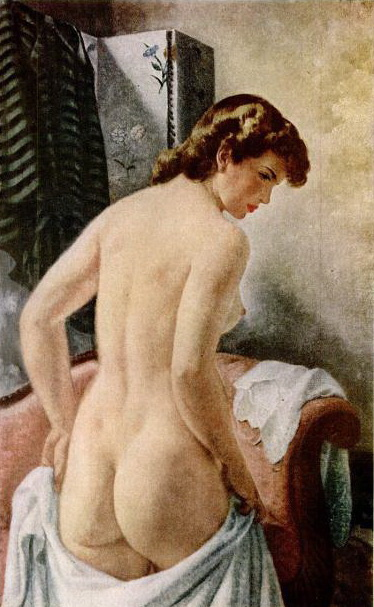
\includegraphics[width=\linewidth]{nudeback}
%       \onelinecaption{{\resizebox{\linewidth}{5.5pt}{\bfseries \hfill NUDE \hfill BACK \hfill SHOWS \hfill  A \hfill DANCER \hfill WHOSE \hfill BACK \hfill SAYS \hfill KROLL, \hfill HAS \hfill BEAUTIFUL \hfill PLANES }}\par}
%       \onelineheader{THE DEAN OF U.S. NUDE-PAINTERS}
%      \begin{multicols}{2}
%      \small
%      \lettrine{A}{t the} age of 63 when businessmen are thinking of retiring leon Kroll according to Life Magazine was having the busiest time of his life, just doing what comes naturally.  \lorem\lorem
%      \end{multicols}
%   \end{minipage}
%\stoptemplate
% 
%
% \newpage
%
%\starttemplate{kroll}
%    \begin{minipage}[b]{0.3\textwidth}
%       \MainHeadera{Sandro Botticelli}
%       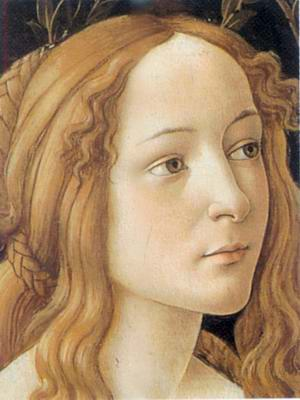
\includegraphics[width=1.0\linewidth]{botticelli-34}\par
%       \byline[BOTTICELLI ]{ painted hundreds of portraits. He is famous for his `Young Woman' series. Even in his larger compositions, he took extreme care of the details of women's faces.}
%   \end{minipage}\hspace*{0.2cm}
%   \begin{minipage}[b]{0.67\textwidth}
%       \putimage[width=\linewidth]{youngwoman}\par
%       \tinyskip
%       \onelinecaption{YOUNG WOMAN}\par
%       \onelineheader{SADRO BOTTICELLI'S PORTRAITS}
%      \begin{multicols}{2}
%      \small
%      \lettrine{A}{t the} age of 63 when businessmen are thinking of retiring leon Kroll according to Life Magazine was having the busiest time of his life, just doing what comes naturally.  \lorem\lorem
%      \end{multicols}
%    \end{minipage}
%\stoptemplate
%
%
%\newgeometry{top=1cm,left=1cm,right=1cm,bottom=1cm}
% \newtheorem{process}{Algorithm}
% \begin{process}
% Test exam
% \end{process}
%\clearpage
%
% \chapter{Posters}
% \makeatletter
%\def\HUGE{\@setfontsize\HUGE{65}{90}}
% \makeatother
%\raggedbottom
%\begin{minipage}{0.8\textwidth}
%\sffamily
%\centering
%\HUGE{\bf SYMPOSIUM}\\
%
%\LARGE{\textbf{\so{CAROLINA DYNAMICS GROUP}}}\\
%
%\Large{\textbf{\so{CLEMSON UNIVERSITY}}}\\
%%\large{\textbf{APRIL 5, 2012}}
%
%\bigskip
%
%\begin{minipage}[b]{0.6\textwidth}
%\normalsize
%\includegraphics[width=\linewidth]{lorenzattractor01}
%
%\textbf{PRESENTED BY THE CAROLINA DYNAMICAL \\ SYSTEMS GROUP}. Some more text here to fill the space. You need to get the reader to stop and read a bit more. Some more text here to fill the space. \par 
%\rule{0pt}{32pt}
%\end{minipage}\hspace{5pt}
%\begin{minipage}[b]{0.37\textwidth}
%\textbf{\large INVITED SPEAKERS}\par
%
%{\leavevmode \raggedright
%Dr Liang Foo\\
%Dr Berry Ling\\
%Dr Zezsko Petrovick \\
%Dr A Berchowitz\\
%\par{}
%}
%
%\medskip
%
%\large{\textbf{VENUE}}
%
%The symposium will take place at Clemson University.
%
%\medskip
%
%{\large\raggedright
%{\textbf{DYNAMICAL SYSTEMS}}
%\par
%}
%\normalsize
%\smallskip
%
%\lorem\lorem\lorem
%
%\medskip
%\textbf{\large ORGANIZERS}\par
%Martin Schmoll, Clemson University\\
%Predrag Punosevac, Augusta State \\
%University
%\medskip
%
%\textbf{\large CONTACT }\par
%
%Predrag Punosevac, Augusta State\\
%University
%\textcolor{blue}{email@mail.com}
%
%\rule{0pt}{78pt}
%\end{minipage}\par
% ^^A\vspace*{-0pt}
%
%\hbox to \textwidth{\HUGE{\bfseries\rmfamily APRIL 5 $\cdot$  2012}}
%\end{minipage}
%
% \restoregeometry
%
%\iffalse
%</package>
%\fi
% \appendix
% \cxset{
%  chapter name = Appendix,
%  section numbering prefix = \thechapter.}
%  
% \chapter{MWE and Testing Macros}
%
% As far as LaTeX is concerned, there is nothing special in styling an appendix. It is either a chapter or a section with a different name. This name in order to allow internationalization is called \lstinline{\appendixname}.
%\bigskip
%
%\begin{tcolorbox}[width=\linewidth]
%\begin{lstlisting}
%\newcommand\appendix{\par
%  \setcounter{chapter}{0}%
%  \setcounter{section}{0}%
%  \gdef\@chapapp{\appendixname}(*@\footnote{The actual literal used for   \textbackslash{appendixname} is defined later on, so that you can customize the language}\label{appendixname}@*)
%  \gdef\thechapter{\@Alph\c@chapter}
%}
%\end{lstlisting}
%\end{tcolorbox}
%\medskip
%
%The code above is only a simplified version of the command. One might need to add more formatting information such as resetting equation numbers, tables and figures and any special floating environments that have their own numbering.
%
%\begin{tcolorbox}[width=\linewidth]
%\begin{lstlisting}
%\renewcommand\appendix{\par
%                \stepcounter{chapter}
%                \setcounter{chapter}{0}
%                \stepcounter{section}
%                \setcounter{section}{0}
%                \setcounter{equation}{0}
%                \setcounter{figure}{0}
%                \setcounter{table}{0}
%                \setcounter{footnote}{0}
%  \def\@chapapp{\appendixname}%
%  \renewcommand\thechapter{\@Alph\c@chapter}}
%\end{lstlisting}
%\end{tcolorbox}
%
% \section{Test macros}
% We provide a series of MWE for testing purposes.
% \subsection{Letter MWE}
% \iffalse
%<*MWE-01>
% \fi
% \subsection{MWE-01, using \texttt{multicol} and \texttt{multitoc}}
%    \begin{macrocode}
%^^A This is an example using the default |lstlisting|
%^^A environment.
\documentclass{article}
\usepackage{phd}
\begin{document}
  \begin{lstlisting}
    \def\test{This is a test.}  
  \end{lstlisting}
  \begin{teX}
    \def\test{This is a test.} 
  \end{teX}
  \begin{teXX}
    \def\test{This is a test.} 
  \end{teXX}
  
  \startnumberat{25}
  \begin{teX}
    \def\test{This is a test.} 
  \end{teX}
  
  \startnumberat{35}
  \begin{teX}
    % coloring comments is done in orange
    \def\test{This is a test.} 
  \end{teX}
\end{document}
%    \end{macrocode}
% \iffalse  
%</MWE-01>
% \fi
% \iffalse
%<*MWE-02>
% \fi
% \subsection{Listings MWE-02}
%    \begin{macrocode}
%% Example using |multitoc|
\documentclass{article}
\usepackage{phd}
\renewcommand{\multicolumntoc}{2}
\title{Typesetting the Table of Contents in Multiple Columns}
\author{Dr Y. Lazarides}
\begin{document}
\maketitle
\tableofcontents
\section{First section}
\begin{multicols}{3}
\lipsum[1-2]
\end{multicols}
\subsection{First subsection}
\subsection{Second subsection}
\subsection{Third subsection}
\subsection{Last subsection}
\section{Second section}
\subsection{First subsection}
\subsection{Second subsection}
\subsection{Third subsection}
\subsection{Last subsection}
\section{Last section}
\subsection{First subsection}
\subsection{Second subsection}
\subsection{Third subsection}
\subsection{Last subsection}
\end{document}
%    \end{macrocode}
% \iffalse  
%</MWE-02>
% \fi
% 
% \subsection{Listings MWE-03}
% 
% \iffalse
%<*MWE-03>
% \fi
%    \begin{macrocode}
%% example for using encoded commands such as guillemets. (If you need
%% shorthands you need to load babel.
%%
\documentclass{article}
\usepackage{phd}
\newcommand{\encone}[1]{{\fontencoding{T1}\selectfont#1}}
\begin{document}
\def\Kt#1{{\encone{#1}} &{\small\ttfamily\string#1}}

\noindent\begin{tabular}{@{}*8l@{}}
\toprule
\Kt\guillemotleft  & \Kt\guilsinglleft & \Kt\quotedblbase & \Kt\textquotedbl \\
\Kt\guillemotright & \Kt\guilsinglright & \Kt\quotesinglbase \\
\bottomrule
\end{tabular}
\medskip

\lipsum[1]
\end{document}
%    \end{macrocode}
% \iffalse  
%</MWE-03>
% \fi
% 
% \iffalse
%<*test-tufte>
% \fi
%    \begin{macrocode}
\documentclass[justified]{tufte-book}
\usepackage{phd}
\begin{document}
\lipsum[1]
\sidenote{\RaggedRight \protect\lipsum[5]}
\centering
\begin{minipage}{5cm}
\RaggedRight

\lipsum[1]
\end{minipage}
\end{document}
%    \end{macrocode}
% \iffalse  
%</test-tufte>
% \fi
%
% \iffalse
%<*test-memoir>
% \fi
%    \begin{macrocode}
% clashes with options
\documentclass{memoir}
\usepackage{phd}
\begin{document}
\lipsum[1]
\end{document}
%    \end{macrocode}
% \iffalse  
%</test-memoir>
% \fi
%
%\iffalse
%<*test-scrartcl>
% \fi
%    \begin{macrocode}
% clashes with options
\documentclass{scrartcl}
\usepackage{phd}
\begin{document}
\lipsum[1]

\[ A = \upalpha r^2/4\]

% check for complaints
$$ A = a + b $$
\end{document}
%    \end{macrocode}
% \iffalse  
%</test-scrartcl>
% \fi
% 
%\iffalse
%<*test-hyphenation>
% \fi
%    \begin{macrocode}
\documentclass{scrartcl}
\usepackage{phd}
\begin{document}
%% Tests if hyphenation routines have been
%% found.
\hsize2cm
\noindent Florida appendix asynchronous
\end{document}
%    \end{macrocode}
% \iffalse  
%</test-hyphenation>
% \fi
%
%\iffalse
%<*test-algorithms>
% \fi
%    \begin{macrocode}
% clashes with options
\documentclass{article}
\usepackage{phd}
\begin{document}
\begin{algorithm}[H]
\SetAlgoLined
\KwData{this text}
\KwResult{how to write algorithm with \LaTeX2e }
initialization\;
\While{not at end of this document}{
read current\;
\eIf{understand}{
go to next section\;
current section becomes this one\;
}{
go back to the beginning of current section\;
}
}
\caption{How to write algorithms}
\end{algorithm}
\IncMargin{1em}
\begin{algorithm}
\SetKwData{Left}{left}\SetKwData{This}{this}\SetKwData{Up}{up}
\SetKwFunction{Union}{Union}\SetKwFunction{FindCompress}{FindCompress}
\SetKwInOut{Input}{input}\SetKwInOut{Output}{output}
\Input{A bitmap $Im$ of size $w\times l$}
\Output{A partition of the bitmap}
\BlankLine
\emph{special treatment of the first line}\;
\For{$i\leftarrow 2$ \KwTo $l$}{
\emph{special treatment of the first element of line $i$}\;
\For{$j\leftarrow 2$ \KwTo $w$}{\label{forins}
\Left$\leftarrow$ \FindCompress{$Im[i,j-1]$}\;
\Up$\leftarrow$ \FindCompress{$Im[i-1,]$}\;
\This$\leftarrow$ \FindCompress{$Im[i,j]$}\;
\If(\tcp*[h]{O(\Left,\This)==1}){\Left compatible with \This}{\label{lt}
\lIf{\Left $<$ \This}{\Union{\Left,\This}}\;
\lElse{\Union{\This,\Left}\;}
}
\If(\tcp*[f]{O(\Up,\This)==1}){\Up compatible with \This}{\label{ut}
\lIf{\Up $<$ \This}{\Union{\Up,\This}}\;
\tcp{\This is put under \Up to keep tree as flat as possible}\label{cmt}
\lElse{\Union{\This,\Up}}\tcp*[r]{\This linked to \Up}\label{lelse}
}
}
\lForEach{element $e$ of the line $i$}{\FindCompress{p}}
}
\caption{disjoint decomposition}\label{algo_disjdecomp}
\end{algorithm}\DecMargin{1em}
\end{document}
%    \end{macrocode}
% \iffalse  
%</test-algorithms>
% \fi
%
%<*test-spacing>
% Uses the package setspace to set the spacing of the
% document.
%    \begin{macrocode}
\documentclass{article}
\usepackage{setspace}
\usepackage{lipsum}
\onehalfspacing
\begin{document}
\title{merry setspace christmas test}
\author{who cares?}
\date{2011-12-19}
\maketitle

\section{dummy}
\lipsum[1]
\subsection{first offspring}
\lipsum[2]
\begin{tabular}{llr}
  a & silly & story about latex \\
  silly & a & story
\end{tabular}
\end{document}
%    \end{macrocode}
%</test-spacing>
%
% \iffalse
%<*settings>
% \fi
%% Some settings
%    \begin{macrocode}
\cxset{nag keys = {l2tabu,%
                   orthodox}}
\cxset{onlyamsmath keys = {warning}}
%    \end{macrocode}
% \iffalse
%</settings>
% \fi
%
% \PrintIndex
%
% \Finale

% \newpage
%
% \section{List of Packages and Usage Statistics}
%
% Table~\ref{tbl:listofpaks} provides a list of the packages loaded as default by |phd|.
% The column describing usage statistics
% is from \url{http://arxmliv.kwarc.info/package_usage.php}. It is by no means an
% indication of overall popularity, but I have used these statistics as an
% guide in selecting what packages to include here in order to at least cover
% the scientific side well.
%
% 
\setcounter{step}{0}
\begingroup
\centering
\begin{longtable}{llp{3.5cm}p{3.5cm}}
\toprule
Ser.  &Usage &Remarks\\
\midrule
\inc &fixltx2e & patches to LaTeX2e&\\
\inc &nag      & nag provides routines to warn
                 user against using outdated
                 packages and commands.           &\\
\inc &nag      & microtype&\\
\inc &onlyamsmath &This package inhibits 
					the usage of 
                plain TEX and 
                on demand of standard
					LATEX math environments. 
					This is useful for class writers 
					who want to force
					their clients to use the environments 
					provided by the amsmath package. &\\
\midrule
\inc &graphicx  &  & \\
\inc &wrapfig   &  & \\
\inc &rotating  &  & \\
\inc &subfig    &  & \\
\inc &xcolor    &  & If loaded by class we skip \\
\midrule
\inc &booktabs  &  & \\
\inc &tabularx  &  &\\
\inc &dcolumn   &  &\\
\inc &longtable &  &\\
\inc &colortabl &  &\\
\inc &multirow  &  &\\
\inc &landscape & &\\
\inc &threeparttable & &\\
\midrule
\inc &array     & &\\
\inc &amsfonts  & &\\
\inc &amsmath   & & (66226)\\
\inc &amssymb   & & (74838)\\
\inc &amsthm    & & (15606)\\
\inc &mathtools & &\\
\inc &stmaryd   & &\\
\inc &xpfeil    & &\\
\inc &extpfeil  & &\\
\inc &euscript  &For calligraphic fonts &\\
\inc &bm        &                       &\\
\inc &bbm       &                       &(2200)\\
\inc &upgreek   &                       & \\
\midrule
\multicolumn{4}{c}{Symbols}\\
\midrule
\inc &latexsym  & &\\
\inc &wasymsym  & &\\
\inc &textcomp  & &\\
\inc &pifont    & &\\
\inc &marvosym  & &\\
\inc &manfnt    & &\\
\inc &bbding    & &\\
\inc &ifsym     & &\\
\inc &eurosym   & &\\
\midrule
\inc &epigraph  & &\\
\inc &siunitx   & &\\
\inc &filecontents & &\\
\midrule
\inc & changepage         & &\\
\inc & keyval             & &\\
\inc & ifmtarg            & &\\
\inc & fp                & &\\
\inc & ifthen             & &\\
\inc & xstring            & &\\
\inc & etoolbox           & &\\
\inc & algorithms         & &\\
\inc & algorithmicx       & &\\
\inc & algorithm2e        & &\\
\midrule
\inc & multicol           & &\\
\inc & multitoc           & &\\
\inc & ragged2e           & &\\
\inc & soul               & &\\
\inc & xspace             & &\\
\inc & ulem               & &\\
\inc & alltt              & &(259)\\
\bottomrule
\inc & idxlayout          & &\\
\bottomrule
\inc & tcolorbox          & &\\
\inc & listings           & &\\
\midrule
\multicolumn{4}{c}{Miscellaneous} \\
\midrule
\inc & fourier/fourier-orns & ornaments/math  &\\
\inc & cclicenses         & &\\
\inc & dirtree            &directory trees &\\
\midrule
\multicolumn{4}{c}{Archaic} \\
\midrule
\inc  &linearA & &\\
\inc  &linearB & &\\
\inc  &cypriot & &\\
\inc  &sarabian & &\\
\bottomrule
\end{longtable}
^^A\captionof{table}{List of packages loaded by the phd package.}
\endgroup

% \label{tbl:listofpaks}
%
\endinput


% ^^A\addtocontents{toc}{\protect\end{multicols}}
%\begin{thebibliography}{1}
%\raggedright
%
%\bibitem{companion}
%Frank Mittelbach et al.:
%\textit{The LaTeX Companion}.\\
%2nd edition. Addison Wesley, 2004.
%
%
%\bibitem{fntguide}
%\LaTeX3 Project Team (Ed.):
%\textit{LaTeX2e font selection.}\\
%CTAN: \path{macros/latex/doc/fntguide.pdf}\\
%(Part of the \LaTeX{} online documentation)
%
%\bibitem{marvosym}
%Thomas Henlich,Mojca Miklavec:
%\textit{The MarVoSym Font Package}
%
% ^^A\end{thebibliography}
%
For custom section
\makeatletter
\renewcommand\thesubsection{\thesection.\two@digits{\value{subsection}}}
\renewcommand\thesubsubsection{\thesubsection.\two@digits{\value{subsubsection}}}
\makeatother

TODO 
http://tex.stackexchange.com/questions/45651/how-do-i-determine-in-which-order-packages-have-been-loaded
% 
%   
% 
% 
%  
%  
%  
%  
%  
%  
%  \cxset{steward,
  numbering=arabic,
  custom = stewart,
  offsety=0cm,
  image=hine06,
  texti={A picture is worth a thousand words, but if you don't add a good description of what it is in a caption, your readers will be left scratching their heads. Here we discuss captions in general as well as the formatting commands available in LaTeX, some common packages and athena.},
  textii={In this chapter we discuss methods that allow the formatting and positioning of captions, based on a set of key values. Central  to this process is the separation of content from presentation.
We also discuss the basic formatting tools that are available and how one can modify them to blend them with the rest of the design.
 }
}
\chapter{Typesetting Captions}
\section{Introduction}

Publications that include figures and tables will normally dictate
the style of captions. Captions, besides normal typography 
requirements such as fonts, can vary in their numbering scheme, can
include a label such as figure or fig they can include a colon or stop
after the label and can be centered hanged or left justified. 
Numbering can also vary; the counters can be reset at every chapter or section or can be continuous. So
there are quite a few options to define in a template.

The formatting commands for the captions key value interface follow the same style of the rest of the package. We use the \pkg{caption} package to provide the interface to the key value settings.


\section{Conventions}

All caption keys start with the word |caption|. The float type follows, so |caption figure font-size| refers to the caption of a \textit{figure environment}. If the word \textit{figure} is omitted the style is applicable to both tables and figures. 

As users will probably only have to set these keys once, my recommendation is to use the longer version that can give you finer control. Also your template will be easier to modify in the future.
\medskip

\keyval{caption format}{\marg{plain|hang}}{This affects all captions such as tables and figures and will produce either a hang caption or with plain will wrap arund the figure number like a normal paragraph.}

\keyval{caption figure format}{\marg{plain | hang}}{Affects ONLY figure captions such as tables and figures and will produce either a hang caption or with plain will wrap around the figure number like a normal paragraph.}

\keyval{caption figure numbering style}{\marg{auto|continuous|reset on sections|custom}}{}
\keyval{caption figure numbering}{arabic,alph,Alph,roman,Roman,custom}{}
\keyval{caption separator}{colon,semicolon,none,custom}{Sets the separator, such as \textbf{:} or a colon or none.}
\keyval{caption label name}{}{}
\keyval{caption before}{}{}
\keyval{caption after}{}{}

\cxset{caption format/.code=\captionsetup[figure]{format=#1}}


\begin{texexample}{}{}
\bgroup
\cxset{caption format = hang}
\captionof{figure}{This is a very long command to see how all
these can wrap in a hang format, if the text is longer than
a paragraph.}
\egroup

\bgroup
\cxset{caption format = plain}
\captionof{figure}{This is a very long command to see how all
these can wrap in a hang format, if the text is longer than
a paragraph.}
\egroup
\end{texexample}

As you can see from the example, the changes can also be localized if
they are within a group.



\def\captionlabelfont@cx{bf}
\cxset{caption font/.code = \captionsetup[figure]{font=#1}}

\cxset{caption font={bf}}




\begin{texexample}{}{}
\cxset{caption format = hang}
\cxset{caption font={bf}}
\captionof{figure}{This is a very long command to see how all
these can wrap in a hang format, if the text is longer than
a paragraph.}
\end{texexample}



\section{Technical discussion}

The formatting of the caption, happens in stages like the sectioning commands.  \lstinline+\@makecaption}+  command is responsible for the typesetting and is defined in the standard LaTeX classes. The \cs{caption} and command is defined in the LaTeX kernel in the 
|float.dtx| class. As always we will start our discussion from the user command and follow it through to the typesetting macros.

When the user command \cs{caption} is processed, LaTeX checks if it is outside a float and if it is issues an error message. It then swallows the argument. It then calls \cs{@caption} which does further processing.


\begin{tcolorbox}
\begin{lstlisting}
\def\caption{%
5 \ifx\@captype\@undefined
6 \@latex@error{\noexpand\caption outside float}\@ehd
7 \expandafter\@gobble
8 \else
9 \refstepcounter\@captype
10 \expandafter\@firstofone
11 \fi
12 {\@dblarg{\@caption\@captype}}%
13 }


\long\def\@caption#1[#2]#3{%
15 \par
16 \addcontentsline{\csname ext@#1\endcsname}{#1}%
17 {\protect\numberline{\csname the#1\endcsname}{\ignorespaces #2}}%
18 \begingroup
        \@parboxrestore
20 \if@minipage
21     \@setminipage
22 \fi
23 \normalsize
24 \@makecaption{\csname fnum@#1\endcsname}{\ignorespaces #3}\par
25 \endgroup}
\end{lstlisting}
\end{tcolorbox}

The \cs{@makecaption} is the main typesetting macro and this is
where we need to hook if we want finer grain of control.


\cxset{label punctuation/.code = \gdef\labelpunctuation@cx{#1}}
\cxset{label space/.code = \gdef\labelhspace@cx{\hskip#1}}

\captionof{figure}{This is a very long command to see how all
these can wrap in a hang format, if the text is longer than
a paragraph.}

\begin{texexample}{}{}

\cxset{caption format = hang}
\cxset{caption font={tt}}
\cxset{label punctuation=?}
\cxset{label space =1.5em}

\captionof{figure}{This is a very long command to see how all
these can wrap in a hang format, if the text is longer than
a paragraph.}

\end{texexample}


\cxset{label punctuation=?}
\captionof{figure}{This is a very long command to see how all
these can wrap in a hang format, if the text is longer than
a paragraph.}

\cxset{label punctuation=:}
\cxset{label space =.5em}
\def\figurename{\textbf{Figure}}

\setlength\abovecaptionskip{10\p@}
\setlength\belowcaptionskip{0\p@}

\long\def\@makecaption#1#2{%
  \vskip\abovecaptionskip
  \sbox\@tempboxa{#1\labelpunctuation@cx #2}
  \ifdim \wd\@tempboxa >\hsize
    #1\labelpunctuation@cx\labelhspace@cx#2\par
  \else
    \global \@minipagefalse
    \hb@xt@\hsize{\hfil\box\@tempboxa\hfil}%
  \fi
  \vskip\belowcaptionskip}

\begin{tcolorbox}
\begin{lstlisting}
\newlength\abovecaptionskip
\newlength\belowcaptionskip
\setlength\abovecaptionskip{10\p@}
\setlength\belowcaptionskip{0\p@}

\long\def\@makecaption#1#2{%
  \vskip\abovecaptionskip
  \sbox\@tempboxa{#1:: #2}
  \ifdim \wd\@tempboxa >\hsize
    #1:: #2\par
  \else
    \global \@minipagefalse
    \hb@xt@\hsize{\hfil\box\@tempboxa\hfil}%
  \fi
  \vskip\belowcaptionskip}
\end{lstlisting}
\end{tcolorbox}

\section{List of Figures}
\begin{tcolorbox}
\begin{lstlisting}
\newcommand\listoffigures{%
    \if@twocolumn
      \@restonecoltrue\onecolumn
    \else
      \@restonecolfalse
    \fi
    \chapter*{\listfigurename}%
      \@mkboth{\MakeUppercase\listfigurename}%
              {\MakeUppercase\listfigurename}%
    \@starttoc{lof}%
    \if@restonecol\twocolumn\fi
    }
\end{lstlisting}
\end{tcolorbox}


In the |phd| package this is set as a property via a key-value interface and hence we can use a normal chapter. If it need be we can define a special chapter style only for this heading. This way we can control all aspects of the formatting of the head.

\begin{macro}{\listfigurename}
The \textit{List of Figures} for example in many Social Sciences books is typed as {List of Illustrations} and also adds credits.
\end{macro}




\begin{figure}[htp]
\includegraphics[width=\textwidth]{listofillustrations}
\caption{List of Illustrations extract from \textit{Oxford History of Art, Portraiture}, Shearer West, Oxford University Press, 2004.}
\end{figure}
\begin{figure}[htp]
\includegraphics[width=0.67\textwidth]{titian}
\centering
\caption{Figure from \textit{Oxford History of Art, Portraiture}, Shearer West, Oxford University Press, 2004. The figures are numbered consecutively and the text in the List of Illustrations have different formatting.}
\end{figure}

\section{Formatting the List of Figures Heading}

LaTeX formats the list of figures heading in a similar manner to that of the Table of Contents. The Title `List of Figures` is obtained from the \cs{listfigurename} and which is also accessible from Babel. It does not add an entry to the ToC.



It is good to know that \cs{captionsetup} has an effect on the current environment only.
So if you want to change settings for the current figure or table only, just place the
\cs{captionsetup} command inside the figure or table right before the \cs{caption}
command.


Many of the caption figures can be changed within LaTeX itself. For example to get continuous numbering in the book class.

\begin{tcolorbox}
\begin{lstlisting}
\makeatletter
\@removefromreset{table}{chapter}
\renewcommand{\thetable}{\arabic{table}}
\makeatother
\end{lstlisting}
\end{tcolorbox}

\begin{macro}{removefromreset}
The command \cs{removefromreset} can be found by loading the \pkg{remreset} package. Other combinations are also possible.
\end{macro}

\subsection{Caption numbering scheme}

The caption numbering scheme key value interface, provides five
options: 
\medskip

\keyval{caption numbering scheme}{\marg{default|continuous| chapter|section}}{The numbering style either continous or reset per spacing etc...}


% Date: Sat, 30 Jul 1994 17:58:55 PST
% From: Donald Arseneau <asnd@erich.triumf.ca>
%
%  |\@removefromreset{FOO}{BAR}| : Removes counter FOO from the list of
%                       counters |\cl@BAR| to be reset when counter BAR
%                       is stepped.  The opposite of |\@addtoreset|.

\def\@removefromreset#1#2{\let\@tempb\@elt
   \expandafter\let\expandafter\@tempa\csname c@#1\endcsname
   \def\@elt##1{\expandafter\ifx\csname c@##1\endcsname\@tempa\else
         \noexpand\@elt{##1}\fi}%
   \expandafter\edef\csname cl@#2\endcsname{\csname cl@#2\endcsname}%
   \let\@elt\@tempb}

\@removefromreset{figure}{chapter}
\renewcommand{\thefigure}{\arabic{figure}}

\@specialfalse\@tocfalse

\begin{texexample}{}{}
\setdefaults
\cxset{chapter opening=anywhere,
          chapter font-size=\normalfont,
          title font-size=\large}


\gdef\continuousfigures@cx{\@removefromreset{figure}{chapter}
\gdef{\thefigure}{\arabic{figure}}}

\cxset{caption numbering continuous/.code={\continuousfigures@cx}}


\chapter{This is the First Chapter}
\captionof{figure}{test}
\captionof{figure}{test}
\chapter{This is the Second Chapter}
\captionof{figure}{test}
\captionof{figure}{test}
\end{texexample}


\begin{figure}[htp]
\includegraphics[width=0.98\textwidth]{captionspecial}
\centering
\caption{Figure from \textit{Oxford History of Art, Portraiture}, Shearer West, Oxford University Press, 2004. The figures are numbered consecutively and the text in the List of Illustrations have different formatting.}
\end{figure}



%  

%  
\let\frogking\lorem

\chapter{Floats}


Most publications contain a lot of figures and tables. There are instances where
a table can be broken across pages, but this is unacceptable for figures. For this reason
figures and short tables need special treatment. The rather naıve method of treating these
objects is to start a new page every time a floating object is too large to fit on the present
page. A more sophisticated method to tackle this problem is to ‘‘float’’ any object that
does not fit on the current page to a later page while filling the current page with text.

This is why these objects are called floating objects. LATEX provides two environments
that are treated as floating objects: the figure and the table environments. Both environments
are written the same way; they differ only in the text that is prepended in the
caption. Moreover, there are two environments that can be used in double column documents
to generate floats that may occupy both columns: the \cs{figure*} and the \cs{table*}
environments. Here is how we can begin a table or a figure:

\begin{teXXX}
 \begin{table}[placement specifier ]
 \begin{figure}[placement specifier]
\end{teXXX}

An optional placement specifier is used to tell LATEX where the float is allowed to be
moved to. The placement specifier consists of a sequence of float placing permissions:

\begin{table}[htbp]
\begin{tabular}{ll}
\toprule
Placement   & position\\
\midrule
h                 & here\\
t                  & top\\
b                 & bottom\\
p                 & on a special page containing only floats\\
\bottomrule
\end{tabular}
\end{table}




Apart from the float placing permissions above there exists a fifth one, namely (!), which
forces LATEX to actually ignore most of the internal parameters related to float placement.
LATEX also provides the command \cs{suppressfloats},which prevents LATEX from putting


\section{The float package}

The \docpkg{float} package provides a friendly interface to define new float objects. Moreover, the package
defines certain ‘‘float styles’’ that can be used to define new floating objects.  It
was designed by Anselm Lingnau. New float objects can be defined with the command

\begin{verbatim}
\newfloat{type}{placement}{ext }[within ]
\end{verbatim}



Here type is the `type'  of the new class of floats (e.g., program, diagram, etc.),
placement gives the default placement specifier, and ext is the filename extension
for the file that will keep the captions in cases wherewewant to have a list of programs,
list of diagrams, or other lists. The optional argument within is used to number float
objects within some sectioning unit (e.g.,chapter, section). Here is a complete example:

\begin{teXXX}
\floatstyle{plain}
\newfloat{Photo}{htbp}{fot}[section]
\end{teXXX}



\makeatletter
%\newcommand\fs@framed{\def\@fs@cfont{\bfseries}\let\@fs@capt\floatc@ruled
%\def\@fs@pre{\hrule height.8pt depth0pt \kern2pt}%
% \def\@fs@post{\kern3pt\hrule\relax}%
% \def\@fs@mid{\kern2pt\hrule\kern2pt}%
% \let\@fs@iftopcapt\iftrue}
%\makeatother


\floatstyle{plain}
\newfloat{Photo}{htbp}{fot}%[section]

\begin{Photo}
 \centering
 \includegraphics[width=0.65\linewidth]{china-05}
\caption[a short caption]{If the caption is very long it is formatted as a paragraph, which is flushleft. If it is short it will be centered. }
\end{Photo}


\begin{Photo}
 \centering
 \includegraphics[width=0.65\linewidth]{china-06}
\caption{. . . caption . . . }
\end{Photo}

\begin{Photo}
 \centering
 \includegraphics[width=0.65\linewidth]{yaleartschool}
\caption{. . . caption . . . }
\end{Photo}



Note that after each such definition, a new 
environment will be available. Naturally,
its name depends on the `type' (e.g., the example code above will create the program
environment). The `float style' can be specified with the \cs{floatstyle} command. The
command takes only one argument, which is the name of a ‘‘float style’’:

\begin{teXXX}
\begin{Example}
     First verbatim line.
     Second verbatim line.
     Third verbatim line.
\end{Example}
\end{teXXX}



\floatstyle{ruled}
\newfloat{Example}{htbp}{loe}[chapter]

 \begin{Example}
 \begin{verbatim}
   \begin{Photo}
      \centering
      \includegraphics[width=0.65\linewidth]{./graphics/level3}
      \caption{. . . caption . . . }
   \end{Photo}
\end{verbatim}
\caption{Example using verbatim code}
 \end{Example}

\begin{Photo}
 \centering
 \includegraphics[width=0.85\linewidth]{old-timer-structural-worker}
\caption{. . . caption . . . }
\end{Photo}

\newlength{\egwidth}\setlength{\egwidth}{0.48\textwidth}

\newenvironment{ega}%
{\begin{list}{}{\setlength{\leftmargin}{0.02\textwidth}%
\setlength{\rightmargin}{\leftmargin}}\item[]\footnotesize}%
{\end{list}}

\newenvironment{egbox}%
{\begin{minipage}[t]{\egwidth}}%
{\end{minipage}}

\newcommand{\egstart}{\begin{ega}\begin{egbox}}
\newcommand{\egmid}{\end{egbox}\hfill\begin{egbox}}
\newcommand{\egend}{\end{egbox}\end{ega}}

% one or two other commands

\newcommand{\fn}[1]{\hbox{\tt #1}}
\newcommand{\llo}[1]{(see line #1)}
\newcommand{\lls}[1]{(see lines #1)}


\egstart
\begin{verbatim}
Here is some advice to remember:
\begin{quotation}
Environments for making
...other things as well.

Many problems
...environments.
\end{quotation}
\end{verbatim}
\egmid%
Here is some advice to remember:
\begin{quotation}
Environments for making quotations
can be used for other things as well.

Many problems can be solved by
novel applications of existing
environments.
\end{quotation}
\egend

The \cs{tabbing} environment overcomes this problem. Within it you set
tabstops and tab to them much like you do on a typewriter.  Tabstops are
set with the |\=| command, and the |\>| command moves to the
next stop.  The
|\\| command is used to separate each line.  A line that ends |\kill|
produces no output, and can be used to set tabstops:


\begin{teX}
\begin{tabbing}
 Income \=Expenditure \= \kill
 Income \>Expenditure \>Result\\
 20s 0d  \>19s 11d \>Happiness\\
 20s 0d  \>20s 1d  \>Misery \\
\end{tabbing}
\end{teX}

\smallskip

\begin{tabbing}
Income \=Expenditure \=    \kill
Income \>Expenditure \>Result \\
20s 0d \>19s 11d \>Happiness   \\
20s 0d \>20s 1d  \>Misery    \\
\end{tabbing}


Unlike a typewriter's tab key, the |\>| command always moves to the next
tabstop in sequence, even if this means moving to the left.  This can cause
text to be overwritten if the gap between two tabstops is too small.



\section{Environment}

\begin{teX}
\def\beginstory{
  \vskip 0.5in                 % Skip down 1/2 before story
   \begingroup                  % Start of formatting properties
   \leftskip 1in\rightskip 1in  % Wider margins for narrower text
   \itshape                     % Italic font
   \noindent{.\dotfill{}.\par}  % Make dotted line
	% Text after close of \beginstory will be story formatted
}

\def\endstory{
  \par\noindent{.\dotfill{}.\par}  % Make dotted line
  \endgroup                        % End of formatting properties
  \vskip 0.5in                    % Skip final 1/2 inch
}

\beginstory 

  Just a short story 

\endstory

\end{teX}



Here's a story about the formative era of personal computing. I
originally wrote it in 1999, but the point it makes is still valid.
Hope you like it.



\subsection*{The \protect\latex way}
LaTeX implements macros |\begin| and |\end|. These are a generic pair whose argument determines the environment that's being begun or ended.

LaTeX makes it much easier to code environments. Here's a generic environment definition:

|\newenvironment{environment_name}{stuff to do before text}{stuff to do after text}|

That's it -- the \cs{newenvironment} macro takes three arguments:
The name of the environment being created
The stuff to do before the text being assigned that environment
The stuff to do after the text being assigned that environment

The resemblance to \tex paired macros is obvious, but \latex  environments make it generic across all environments, and place the beginning and ending code in one place. Not only that, but because the environment has one name instead of two different names, it's very easy for a front end like LyX to assign environments to highlighted stretches of text.

The |\newenvironment|  macro works only when the environment name is undefined. If there's already an environment with that name, use|\renewenvironment|  instead. If you don't know, there are ways to test.

The following is a LaTeX version of the |\beginstory| \ldots | \endstory| example, with the two macros folded into the definition of one environment called story.


Lamport, cleverly defined macros that automatically, create the necessary \tex \cs{begingroup} and \cs{endgroup} commands. You can find the code in the |source2e| file and which is shown below:\footnote{You can find the full code in \texttt{File y, for ltmiscen.dtx}}

\begin{teX}
\def\begin#1{%
  \@ifundefined{#1}%
  {\def\reserved@a{\@latex@error{Environment #1 undefined}\@eha}}%
  {\def\reserved@a{\def\@currenvir{#1}%
  \edef\@currenvline{\on@line}%
  \csname #1\endcsname}}%
  \@ignorefalse
  \begingroup\@endpefalse\reserved@a}


\def\end#1{%
  \csname end#1\endcsname\@checkend{#1}%
  \expandafter\endgroup\if@endpe\@doendpe\fi
  \if@ignore\@ignorefalse\ignorespaces\fi}
\end{teX}

In \latex environments are defined as 
|\begin{foo}| and |\end{foo}| which are are used to delimit environment |foo|.
|\begin{foo}| starts a group and calls |\foo| if it is defined, otherwise it does
nothing.

|\end{foo}| checks to see that it matches the corresponding |\begin| and if so,
it calls |\endfoo| and does an |\endgroup|. Otherwise, |\end{foo}| does nothing.
If |\end{foo}| needs to ignore blanks after it, then |\endfoo| should globally set
the |@ignore| switch true with |\@ignoretrue| (this will automatically be global).

NOTE: |\@@end| is defined to be the |\end| command of TEX82.
|\enddocument| is the user's command for ending the manuscript file.
|\stop| is a panic button to end \tex in the middle.


\section*{Checking the environment}

This is interesting in that we can use \cs{@currenvir} to check if a command is within a particular environment. The following code will be used to typeout the environment.

\begin{teX}
\begin{enumerate}
   \item Check environment with |@currenvir|
   \makeatletter
   \item The current environment is \@currenvir
   \makeatother
\end{enumerate} 
\end{teX}

\begin{enumerate}
\item Check environment with |@currenvir|
\makeatletter
 \item The current environment is \@currenvir
\makeatother
\end{enumerate}

The \cs{@checkend} \index{Latex kernel!@checkend} uses the \cs{@currenvir}\index{Latex kernel!@currenvir} to see if there is a matching
begin environment and if it cannot find it produces an error.

\begin{teX}
\def\@checkend#1{%
   \def\reserved@a{#1}
   \ifx\reserved@a\@currenvir 
   \else
     \@badend{#1}
   \fi
}
\end{teX}

It is a pity that there is no real guide for explaining the \latex macros, other than just reading through them. Lamport and later his associates managed to produce code that offers the user a friendly API. Besides the scenes of this API, it also offers the package writers hundreds of useful commands.






%  
%	\makeatletter \cxset{toc image = \@empty}
\chapter{GROUPING AND SCOPING RULES}
\index{Grouping}
\label{ch:grouping}

Like most computer languages \tex\ has a grouping mechanism that is able to confine most changes to a particular locality. This chapter explains what sort of actions can be local, and how groups are formed.
\medskip

\DescribeMacro{\bgroup}
       Implicit beginning of group character.

\DescribeMacro{\egroup} Implicit end of group character.

\DescribeMacro{\begingroup} Open a group that must be closed with |\endgroup|.

\DescribeMacro{\endgroup} Close a group that was opened with |\begingroup|.

\DescribeMacro{\aftergroup} Save the next token for insertion after the current group ends.

\DescribeMacro{global} Make assignments, macro definitions, and arithmetic global.

\DescribeMacro{globaldefs} Parameter for overriding |\global| prefixes. IniTEX default: 0.



The grouping mechanism can be thought of a bit like scope in other programming languages, with the
exception that in \tex the mechanism is much more Pascal-like. Most assignments made inside a group are local to that group
unless explicitly indicated otherwise, and outside the group old values are restored (pretty much like in Pascal). If we type the following  example:

\begin{texexample}{}{}
\def\i{42}
{
   \def\i{43}
   \def\b{2}
}
The value of the \textbackslash i is now \i

\def\x{a}
\let\y\x
\bgroup
  \def\x{b}
  Within group \x\par
\egroup
  Outside group \x
\end{texexample}

we get   \texttt{The value of the \textbackslash i is now 42}. Due to the way \tex scoping rules work, the old program state
will be restored \textit{completely} after returning from the local group. Neither the change to |\i| nor the definition of |\b| will survive. This is also true for register changes or other assignments.

The listing above defines |\i| enters a local scope (a \tex group) and changes |\i|

The |\end| command is allowed to occur inside a group, but TEX will give a diagnostic
message about this.

The \cs{aftergroup} control sequence saves a token for insertion after the current group. Several
tokens can be set aside by this command, and they are inserted in the left-to-right order in which
they were stated.

\begin{texexample}{}{}
\def\x#1;{#1}
\def\y{15}
{\globaldefs1
\bgroup
   \def\y{0}
   \aftergroup\x\aftergroup\y\aftergroup;
   \aftergroup}
\egroup
\y


\globaldefs0

\def\z{1}
{\def\z{0}
\z
}

\z

\end{texexample}

\begin{texexample}{}{}
{ \def\z{1}
  {\def\z{0}\globaldefs1
     \z
    {
	\z
    }
   \z
  }
 \z
}





\end{texexample}



\section{Local and global assignments}

An assignment or macro definition is usually made global by prefixing it with \cs{global}, but nonzero
values of the integer parameter |globaldefs| override |doccmd{global}|
is positive every assignment is implicitly prefixed with \doccmd{global}, and if |\globaldefs| is negative,
|\global| is ignored. Ordinarily this parameter is zero. It has very
limited use and even in the \latex\ kernel we can only find 3-4 uses when defining math fonts.


Some assignment are always global: the \marg{global} assignments are:

font assignment assignments involving \cs{fontdimen}, \cs{hyphenchar}, and \cs{skewchar}.

hyphenation assignmenti \cs{hyphenation} and \cs{patterns} commands.

hbox size assignmenti altering box dimensions with \cs{ht}, \cs{dp}, and \cs{wd} 

hinteraction mode assignmenti run modes for a \tex job (see Chapter 32).

hintimate assignmenti assignments to a hspecial integeri or hspecial dimeni;


\section{Braces}

The most common way to group is to use braces. They are used for two purposes:

\begin{enumerate}
\item to indicate the start and end of a group. For example |{\small here is some text}|.

\item to indicate that a string of tokens should be treated as one unit. For example in |\def\abc{...}| the braces are used
to delimit the argument.
\end{enumerate}

It is important to note that the characters \{, \} are not hardwired in \tex. Any tokens with catcodes 1 and 2 can be used.
The plain format starts [343] by saying:

\begin{teX}

\catcode`\{ =1
\catcode `} = 2
\end{teX}

Tokens with catcodes 1 and 2 are called \emph{explicit braces}. An \emph{implicit} brace is a control sequence whose replacement text is an explicit brace. Thus the two |plain| control sequences 
|\bgroup| and |\egroup| are implicit braces. They are defined in [353] by:

There is also a low-level \tex operator pair for creating groups. It works
just as the braces. A group is started with \cs{begingroup} and ended with
\cs{endgroup}. These operators may be freely mixed with braces but pairs
should be properly matched. So ��|{ \begingroup \endgroup }|�� is allowed
but ��|{ \begingroup } \endgroup|�� is not.

\begin{teX}
\let\bgroup={
let\egroup=}
\end{teX}

They can be used where unbalanced braces are needed.

Salomon gives an example to typeset a number of paragraphs with a negative indentation\footnote{This style can sometimes be found in old books.}:

\begin{teX}
\def\negIndent{\brgoup\parindent=-20pt}
\def\endIndent{\par\egroup}

\negIndent
  \small\lipsum[1]
\endIndent
\end{teX}

This will typeset:

\def\beginindent{\bgroup\parindent=-20pt}
\def\endindent{\par\egroup}

\beginindent
  \small\lipsum[1-3]
\endindent


The other two primitives \cs{begingroup} and \cs{endgroup} can also be used to define a group. However a group that starts with a |begingroup| must end with an |\endgroup|. This provides a mechanism for error checking, which \tex's parsing routines can easily catch.

Note that |\begingroup| and |\endgroup| can only be used to define a group, not to delimit a string. You can say:

\begin{teX}
\begingroup
  \it abc
\endgroup
\end{teX}

but the following will get \tex to complain about missing braces

\begin{teX}
\hbox\begingroup\it abc\endgroup
\end{teX}



\section*{Examples}
From the TexBook Exercise 7.4

Suppose that the commands
\begin{texexample}{}{}
{\catcode`\<=1 \catcode`\>=2
 \bfseries test
>
 test
\end{texexample}

appear near the beginning of a group that begins with |{| these specifications instruct
TEX to treat |<| and |>| as group delimiters. According to \tex's rules of locality, the
characters |<| and |>| will revert to their previous categories when the group ends. But
should the group end with |}| or with |>| ?

It ends with either |>| or |}| or any character of category 2; then the effects of all
\cs{catcode} definitions within the group are wiped out, except those that were global.
\tex  doesn't have any built-in knowledge about how to pair up particular kinds of
grouping characters. New category codes take effect as soon as a |\catcode| assignment
has been digested. For example,

\begin{teX}
{\catcode`\>=2 >
\end{teX}

is a complete group. But without the space after |2|  it would not be complete, since TEX
would have read the |>|  and converted it to a token before knowing what category code
was being specified; \tex always reads the token following a constant before evaluating
that constant.

\topline

\textbf{Example}: \textsc{Adjusting the spacing of a font} An interesting example that illustrates some of the concepts that were discussed so far is to try and change the \textit{inter word spacing} of text using the \cs{fontdimen2} parameter. The interesting aspect of this example is that
we want to change the spacing, but since the font changes are global, we want to revert back to the original font at the end of the group. Although there are many other ways of achieving this we will use the \cs{aftergroup}.

\begin{teX}
\font \roman=cmr10
\font\specroman=cmr10
%% Next, the special registers
\newdimen\savedvalue
\savedvalue=\fontdimen2\roman
\newdimen\specialvalue
\specialvalue=13.0pt
%% Finally, definitions.
\def \rm{%
  \fontdimen2\roman=\savedvalue }
\def\specrm{%
  \aftergroup\restoredimen
  \fontdimen2\specroman=\specialvalue
  \specroman  }
\def\restoredimen{%
\fontdimen2\roman=\savedvalue }
\end{teX}
{
%% First, fonts.
\font \roman=cmr10
\font\specroman=cmr10
%% Next, the special registers
\newdimen\savedvalue
\savedvalue=\fontdimen2\roman
\newdimen\specialvalue
\specialvalue=13.0pt
%% Finally, definitions.
\def \rm{%
  \fontdimen2\roman=\savedvalue }
\def\specrm{%
  \aftergroup\restoredimen
  \fontdimen2\specroman=\specialvalue
  \specroman  }
\def\restoredimen{%
\fontdimen2\roman=\savedvalue }


{\bf Spaced Out Text} 
\medskip
{\specrm \lorem} dimension2 the interword   value \the\fontdimen2\font


{\bf  Back to Normal}
\medskip

\rm
\lorem

}

This is a test \\{item}
\section{Summary}
\relax\bgroup\relax\egroup\relax 


\section*{Scoping Rules for boxes}

The scoping rules for boxes work similarly to those for other command sequences, since they are just macros defined by \latex or |plain|. In the example below, we define a box |\mybox| and we save a sentence both in global scope as well as local scope.

\begin{teX}
\documentclass{article}
\begin{document}
  \newsavebox{\mybox}
  \savebox{\mybox}{Outside scope}
  \usebox\mybox
  \begin{minipage}{5cm}
    \sbox{\mybox}{from first minipage}(*@ \label{global} @*)
    \usebox\mybox
  \end{minipage}
  \usebox{\mybox}
\end{document}
\end{teX}


This will typeset:
\medskip

\newsavebox{\myboxi}
\savebox{\myboxi}{\tt > Outside scope}

\noindent\usebox\myboxi

\noindent\begin{minipage}{5cm}
\sbox{\myboxi}{\tt > from first minipage}
\noindent\usebox\myboxi
\end{minipage}

\noindent\usebox{\myboxi}


\medskip 
Changing line [\ref{global}] to |\global\sbox| will make the definition of |\mybox| within the minipage environment global and would change the output to:
\medskip



To save memory space, box registers become empty by using them: \tex assumes
that after you have inserted a box by calling |\boxnn| in some mode, you do not need the contents of that register any more and empties it. In case you do need the contents of a box register more
than once, you can |\copy| it. Calling |\copynn| is equivalent to |\boxnn| in all respects except that the register is not cleared.


There are 256 box registers, numbered 0–255. Either a box register is empty (‘void’), or it contains
a horizontal or vertical box. This section discusses specifically box registers; the sizes of boxes,
and the way material is arranged inside them, is treated below.




\newbox\MyBox

\setbox\MyBox=\hbox{\hfil Test\hfill}

\unhbox\MyBox


\noindent\unhbox\MyBox

\noindent{\hfill Test \hfill}



\framebox{\parbox{\linewidth}{\color{black}
\textbf{\textcolor{purple}{\textsf{CAUTION}}}
\begin{enumerate}
\itemsep-5pt
\item \latex will not empty a box as it uses the copy command in the definition of the newsavebox.
\item It is better to use \LaTeX\ commands rather than \tex primitives, when defining boxes, as \latex tests for duplication of names - which is very important if a user uses a lot of different packages.
\item Give always preferences to local definitions rather than global. Globals always create maintenance problems in programming.
\end{enumerate}
}}


\section{Implicit Grouping}

There are  instances where grouping is \textit{implicit}. What this means is that \text starts and ends a group automatically and without any action by the user. There are two major cases where this happens:

\begin{enumerate}
\item The text inside a box such as |\hbox|, |\vbox|, |\vtop|, |\vcenter| etc. is automatically treated by \tex as a group.  For example |\hbox{\bf My Heading}|, will print  \hbox{\bf My Heading}  and it will not continue with the bold font once outside the group. All these commands have curly brackets and these curly brackets form implicit groups.
\item In five cases \tex forms implicit groups. In some of these cases not even curly braces are involved.
\end{enumerate}

\begin{enumerate}
\item The text inside math mode is treated as a group. This is true both for inline math as well as display math.
\item Matching |\left| and |\right| primitives treat the formula in between them as a group.
\item Fractions are treated as a group.
\item The execution of an ouput routine is implicitly enclosed in a group.
\item Columsn in |\halign| based tables are local.
\end{enumerate} 

\subsection{\texttt{afterssignment and grouping}}

The primitive |\afterasignment| does not follow grouping in that it does not save the definition of a token when |\afterassignment| is executed. Consider the following example:

Define the two macros |\xx| and |\yy|.

\def\xx{\string\xx\ executed\par }

\def\yy{\string\yy\ executed\par }

\afterassignment\xx

We start a group, where we have two definitions of |\xx| and |\yy|

{
  \def\xx{\string\xx executed inside a group\par}

  \def\yy{\string\yy executed inside a group\par}

The second afterassignment is execute

  \afterassignment\yy

The group is ended

}


Note afterassignment saves the token following afterassignment without expanding it. Nothing happens until after the next assignment; immediately after the next assignment the saved token is expanded. This is a bit of a tricky part and you can go over it to make sure you understand it well.



Assign a value or define a macro.




































  
%  \makeatletter
% 
%  \chapter{maths}

\parindent1em

\cxset{subsection indent=0pt}\renewsubsection

\starttemplate{kroll}
\thispagestyle{empty}
    \begin{leftcolumn}
         {{\centering \huge  THE ART OF \\
       TYPESETTING\\
       MATHS\\}}
      \medskip
       {\justifying \small Perhaps some day a typesetting language will become standardized to the 
point where papers can be submitted to the American Mathematical Society 
from computer to computer via telephone lines. Galley proofs will not be 
necessary, but referees  and / or copy editors could send suggested changes to 
the author, and he could insert these into the manuscript, again via telephone.\par
\hfill \textit{Donald Knuth}}
\medskip
       \putimage[width=1.0\linewidth]{halmos}\par
       \aheader{shows Kroll at 59. Says he. ``Painting is fascinating'' even when motif my own mug.}
   \end{leftcolumn}
   \begin{rightcolumn}
       \putimage[width=\linewidth]{themathematician}
       \onelinecaption{{\resizebox{\linewidth}{5.5pt}{\bfseries The Mathematician (1918) an oil painting by the Mexican artist Diego Rivera. }}\par}

     \vspace*{1.5\baselineskip}

  \centerline{\onelineheader{TYPESETTING MATHEMATICS}}
      \begin{multicols}{2}
     
      \lettrine{M}{ost people} discover, \alltex when they are faced with the production of a thesis or paper that includes lots of
mathematical text. It is the rais\`on detrait for \tex. In this chapter we will discuss the typesetting of mathematics, common pitfalls and solutions. We will also review some typographical questions.
\parindent1em

You can start writing mathematical text, without any additional loading of packages, either in plain \tex or \latex. The reality is that most institutions have developed their own styles and common packages used by AMS have found widespread use. We will discussing these extensively, but first let us look at how to enter mathematical text. 

To enter mathematical text in plain \tex you just use the |$|\ldots|$| for inline math and |$$|\ldots|$$| for displayed math. \latex uses |\(|
and |)| for inline and |[\]|.
      \end{multicols}
   \end{rightcolumn}
\stoptemplate


\newgeometry{left=3cm,right=3cm, bottom=2cm}
\pagestyle{headings}
\normalfont

\section{Inline and Display Math}
Mathematical typesetting involves either inline math formulae, which are part of a paragraph of text or display math which are a block of mathematical material. \tex will typeset inline math by enclosing the material between  \$\ldots\$. See Example~\ref{ex:inline}.
\bigskip

\begin{texexample}[]{Inline and Display Math}{ex:inline}
This is an inline equation \(a^2+b^2=c^2\)

And this equation is a display equation:
\[a^2+b^2=c^2\]
\end{texexample}


The above code, is valid in \latex and its variants as well. However in certain cases, especially for displayed math, this can introduce some blank lines. Lamport redefined
the \$\$. For inline math use |\(...\)| and for display math |\[...\] |. The above example can be written as:
\bigskip

\begin{texexample}{The Math Environment}{ex:mathenvironment}
 This is an inline equation \(a^2+b^2=c^2\)

 And this equation is a display equation:
 \[a^2+b^2=c^2\]

 \begin{math}
 \sum_{i=1}^{n}i=\frac{1}{2}n\cdot(n+1)
 \end{math}
\end{texexample}



As you can observe the output remains the same.  Spaces within  maths environment are ignored, so use this to your advantage when writing maths. As mentioned earlier, we can use |\[...\]| for display math.


\section{Displayed Equations}


Displayed equations, can either be displayed \emph{flushed left} or \emph{centered}, depending on the option loaded with the standard classes, for example in article use,

\begin{teX}
\documentclass[imperial,11pt,openany, twoside,fleqn]{article}
\end{teX}

We will see, how to change the formatting a bit later on.

\section{Greek letters}

Mathematicians and Engineers, quickly run out of symbols to use with their equations and hence use Greek letters. All
the Greek letters are available in \tex{} 

\begin{table}[htbp]
\centering
\begin{tabular}{llllllll}
\toprule
$\alpha$  &\doccmd{alpha} &$\beta$ &\doccmd{beta} &$\gamma$ &\doccmd{gamma} &$\delta$ &\doccmd{delta}\\
$\epsilon$  &\doccmd{epsilon} &$\varepsilon$ &\doccmd{varepsilon} &$\zeta$ &\doccmd{zeta} &$\eta$ &\doccmd{eta}\\
\bottomrule
\end{tabular}
\end{table}


Sometimes accents are put above or below symbols. The control words used for accents
in mathematics are different from those used for normal text. The normal text control words
may not be used for mathematics and vice-versa.\footnote{\texbook 135-136 }. See also
\href{mathmode.pdf}{http://www.tex.ac.uk/tex-archive/info/math/voss/mathmode/Mathmode.pdf}

\section{Fractions}

There are two ways of typesetting a fraction in \tex{}: it can be typeset as $1/4$ or in the form $\frac{1}{4}$. The first case is entered with no special control characters that is,  \verb+ $1/2$+. The second case is just entered with the control word \cmd{over}.  Hence\verb+ ${1} \over {4}$+ gives ${1} \over {4}$. \LaTeX\ provides a macro \cmd{frac}.

A more complex example,

\begin{texexample}{Fractions}{ex:fractions}
\[
a+\gamma \over \delta^2
\]

\end{texexample}


One complication with using maths in-line with text is that of using different type of fonts. There is a very useful and interesting discussion regarding this in the package \pkg{xfrac}. 

\begin{quotation}
 One of the first exercises in \emph{The \TeX Book} is to design a
 macro for split level fractions. The solution presented is fairly
  simple, using a \emph{virgule} (a slash) for separating the two
  components. It looks okay because the text font and math font of
  Computer Modern look almost identical.\index{virgule}

  The proper symbol to use instead of the virgule is a \emph{solidus}\footnote{The solidus (/)} \index{solidus} is a punctuation mark used to indicate fractions including fractional currency. It may also be called a shilling mark, an in-line fraction bar, or a fraction slash. Its Unicode encoding is \texttt{U+2044}.
\end{quotation}

The solidus is similar to another punctuation mark, the slash, which is found on standard keyboards; the slash is closer to being vertical than the solidus. These are two distinct symbols that traditionally have entirely different uses. However, many people no longer distinguish between them, and when there is no alternative it is acceptable to use the slash in place of the solidus.
Both the ISO and Unicode designate the solidus as \texttt{FRACTION SLASH U+2044} and the slash as \texttt{SOLIDUS U+002F}. This contradicts long-established English typesetting terminology (See Bringhurst).
  which does not exist in Computer Modern. It is however available in
  the European Computer Modern fonts, but I'll get back to that.

Wills also notes in the |xfrac| documentation package the limitations
of the |nicefrac| package:

\begin{quotation}
  The most common way to produce split level fractions within \LaTeX\
  is by means of the \docpkg{nicefrac} package. Part of the reason it
  has found widespread use is due to the strange design of the
  built-in text fractions of the EC fonts, which look like this:
  \textonehalf. 
\end{quotation}

The package is very simple to use but there are a few
issues:

 \begin{itemize}
  \item It uses the virgule instead of the solidus.
  \item Font size of numerator and denominator is bigger than in the
    built-in symbol. Compare Palatino: \switch{ppl}{\nicefrac{1}{2}}
    vs. \switch{ppl}{\textonehalf }. (\sfrac{1}{2})

  \item It doesn't correct for fonts using text figures such as in the
    \docpkg{eco} package. Compare \switch{cmor}{\nicefrac{1}{2}} and
    \switch{cmor}{\nicefrac{8}{9}}.
  \item In math mode, it doesn't always pick up the correct math
    alphabet.
 \end{itemize}

In short: \docpkg{nicefrac} doesn't attempt to be the answer to
everything and so this is not a criticism of the package. It works
quite well for Computer Modern which was pretty much what was widely
available at the time it was developed. Users these days, however,
have a choice of many fonts when they write their documents.

With |xfrac| we can switch fonts easily

 ``You take \sfrac[cmr2]{1}{2} cup of sugar, \ldots''

This is more of an issue if you are going to use |XeLaTeX| and 
you are after specific fonts.


\section{Square roots}

The square root sign, historically derived from a dot but is now simply typeset in the familiar square root symbol.  it is only necessary to use the construction \cs{sqrt}. Hence

\begin{texexample}{Square Roots}{}
$\sqrt{x^2+y^2}$
\end{texexample}

will give $\sqrt{x^2+y^2}$


Notice that \tex takes care of the placement of
symbols and the height and length of the radical. To make cube or other roots, the control
words \cs{root} and \cs{of} are used.  

\begin{texexample}{}{}
   $\root n \of  {1+x^n}$ 
\end{texexample}

\begin{macro}{\surd}
 A possible alternative is to use the control word \cs{surd}; the input  \verb+ \( \surd 2 \)+ will
produce \(\surd 2\). When typesetting square roots care should be taken, to use struts appropriately to get the sizing right.
\end{macro}


\section{Trigonometric and other Functions}

There are several types of functions that appear frequently in mathematical text. In
an equation like $\sin2x+\cos2x=1$ the trigonometric functions \cs{sin} and \cs{cos} are in
roman rather than italic type. This is the usual mathematical convention to indicate that
it is a function being described and not the product of three variables. The control words
\cs{sin} and \cs{cos} will use the right typeface automatically. Here is a table of these and some
other special functions:

\begin{texexample}{Trigonometric Functions}{}
\begin{math}
\sin, \cos, \tan, \cot, \sec, \csc, \arcsin, \arccos,
\arctan \sinh \cosh \tanh \coth \lim \sup \inf
\end{math}

\begin{math}
\limsup \liminf \log \ln \lg \exp \det \deg
\dim \hom \ker \max \min \arg \gcd \Pr
\end{math}

\begin{math}
\cos(2\theta) = 2 \cos^{2}2 \theta-1
\end{math}
\end{texexample}

Functions that are missing from a basic installations can be either defined or one can use one of the many packages that supplement the above.


\section{Using special symbols}

Special symbols such as dingbats loaded using the |pifont| package need to be encloded within an |\mbox| in order to be able to display the glyph properly.
\bigskip

\begin{texexample}{Using special dingbat symbols}{}
\label{e14}
 We start by showing that the function $f(x)=x^2$ is
continuous over the set $X_2$\label{p:X2} defined as the interval
$[0,1]$ where numerals $\frac{i}{\mbox{\ding{172}}}, 0 \le i \le
\mbox{\ding{172}},$ are used to express its points in units $\mu$.
First of all, note that the set $X_2$ is continuous in   $\mu$
because its points are equidistant with the distance
$d=\mbox{\ding{172}}^{-1}$. Since this function is strictly
increasing,  to show its continuity it is sufficient to check the
difference $f(x)-f(x^{-})$ at the point $x=1$. In this case,
$x^{-}=1-\mbox{\ding{172}}^{-1}$ and we have
\[
 f(1)-f(1-\mbox{\ding{172}}^{-1})=
 1-(1-\mbox{\ding{172}}^{-1})^2 =
 2\mbox{\ding{172}}^{-1}(-1)\mbox{\ding{172}}^{-2}.
\]
This number is infinitesimal, thus $f(x)=x^2$ is continuous over
the set $X_2$. \hfill $\Box$
\end{texexample}

\cs{Box}
Notice the use of the |\Box| command to draw a square for  end of proof symbol. This is from the amsmath package. The box is placed at the end of the line using |\hfill $\Box$|.



\section{Partial derivatives}

Partial derivatives can be typeset using the \latex{} command \cs{partial}

\begin{texexample}{}{}

\[
dS = \frac{\partial S}{\partial x}\, dx
   + \frac{\partial S}{\partial y}\, dy
   = \left(y - \frac{2V}{x^2}\right) dx
   + \left(x - \frac{2V}{y^2}\right) dy.
\]
\end{texexample}




\section{Binomial Coefficients}

To typeset binomial coefficients or similar structures, use the command
\cmd{binom} from \docpkg{amsmath}:\index{amsmath!binom}

Pascal's rule can be typeset as:


\begin{texexample}{Binomial Distribution}{ex:binomial}
\[
\binom{n}{k} =\binom{n-1}{k}
+ \binom{n-1}{k-1}
\]
\end{texexample}



\section[SYMBOLS AND ABBREVIATIONS.]{SYMBOLS AND ABBREVIATIONS.}

\label{abbr}\label{symbols}%

\newlength{\dentwidth}\setlength{\dentwidth}{\textwidth}
\addtolength{\dentwidth}{-\parindent}


 \def\Par{%
   \mathchoice
      {\@parallelogram\scriptsize}%
      {\@parallelogram\scriptsize}%
      {\@parallelogram\tiny}%
      {\@parallelogram\tiny}}
\def\@parallelogram#1{%
  \textnormal{\setbox\z@\hbox{#1/}\dimen@\wd\z@
   \@tempdima 2.45\dimen@
   \vbox{\offinterlineskip
      \hbox{\kern.8\dimen@\vrule\@width\@tempdima\@height.4\p@}%
      \kern-.0\p@
      \hbox to\@tempdima{#1/\hfil\rlap/}%
      \kern-.5\p@
      \hbox{\kern.1\dimen@\vrule\@width\@tempdima\@height.4\p@}}}}

\begin{tabular*}{\dentwidth}{rl@{\extracolsep{\fill}}l@{\extracolsep{0pt}}@{\dots}l}

$>$ & is (or are) greater than. & Def. & definition. \\
$<$ & is (or are) less than. & Ax. & axiom. \\
$\Bumpeq$ & is (or are) equivalent to. & Hyp. & hypothesis. \\
$\therefore$ & therefore. & Cor. & corollary. \\
$\perp$ & perpendicular. & Scho. & scholium. \\
$\perp_s$ & perpendiculars. & Ex. & exercise. \\
$\parallel$ & parallel.\qquad $\parallel_s$ parallels. & Adj. & adjacent. \\
$\angle$ & angle.\qquad $\angle_s$ angles. & Iden. & identical. \\
$\triangle$ & triangle.\qquad $\triangle_s$ triangles. & Const. & construction. \\
$\Par$ & parallelogram. & Sup. & supplementary. \\
$\Par_s$ & parallelograms. & Ext. & exterior. \\
$\odot$ & circle.\qquad $\odot_s$ circles. & Int. & interior. \\
rt. & right.\qquad  st.\ straight. & Alt. & alternate. \\
\end{tabular*}

\hbox{\qed\ stands for quod erat demonstrandum, \emph{which was to be proved}.\hss}

\newcommand{\qef}{\textsc{q.e.f.}}
\qef\ stands for quod erat faciendum, \emph{which was to be done.}

The signs $+$, $-$, $\times$, $\div$, $=$, have the same meaning as in Algebra.




\section{Matrices}


\begin{texexample}{Matrices}{ex:matrices}
\[
\mathbf{X} = \left(
\begin{array}{ccc}
x_1 & x_2 & \ldots \\
x_3 & x_4 & \ldots \\
\vdots & \vdots & \ddots
\end{array} \right)
\]
\end{texexample}

The example \ref{ex:bmatrix} illustrates the typesetting of a bracketted matrix hence \ul{b}matrix. If you want the matrix equation to be numbered enclose it withn an |equation| or |gather| environment. In this documentation we have let the |equation| environment to |gather| hence it will make no difference which ever is used.

\begin{texexample}{Bmatrix}{ex:bmatrix}
\begin{equation}
\begin{matrix}
1 & 2 \\
3 & 4
\end{matrix} \qquad
\begin{bmatrix}
p_{11} & p_{12} & \ldots & p_{1n} \\
p_{21} & p_{22} & \ldots & p_{2n} \\
\vdots & \vdots & \ddots & \vdots \\
p_{m1} & p_{m2} & \ldots & p_{mn}
\end{bmatrix}
\end{equation}
\end{texexample}



\subsection{vmatrix}

\begin{texexample}{vmatrix}{ex:vmatrix}

\begin{gather}
\begin{vmatrix}
aa' + bb' + cc' & ea' + fb' + gc' \\
ae' + bf' + cg' & ee' + ff' + gg'
\end{vmatrix}
{} = \begin{vmatrix}
a & b \\
e & f
\end{vmatrix}  \begin{vmatrix}
a' & b' \\
e' & f'
\end{vmatrix} + \begin{vmatrix}
a & c \\
e & g
\end{vmatrix}  \begin{vmatrix}
a' & c' \\
e' & g'
\end{vmatrix}.
\end{gather}
\end{texexample}





\section{Single equations that are too long}

In many cases equations need to be written over two or more lines. The \docpkg{amsmath} package, provides environments that are suitable for this:


\begin{texexample}{The multiline amsmath environment}{ex:multiline}
\begin{multline}
   a + b + c + d + e + f+ g + h + i  + k + l + m + n + o + p\\
              = j + k + l + m + n +\cos^{2}-1
\end{multline}
\end{texexample}



\newpage


\section{array environment}
This is simply the same as the eqnarray environment only with the possibility of
variable rows and columns and the fact, that the whole formula has only one
equation number and that the array environment can only be part of another math
environment, like the equation environment or the displaymath environment. With
@{} before the first and after the last column the additional space |\arraycolsep| is
not used, which maybe important when using left aligned equations.

\begin{tcblisting}{colback=blue!5,boxrule=2pt,colframe=blue!75!black,title=\textbf{The egnarray Environment},width=1.05\textwidth}
\begin{eqnarray}
a & = & b + c \\
& = & d + e + f + g + h + i
+ j + k + l \nonumber \\
&& +\: m + n + o \\
& = & p + q + r + s
\end{eqnarray}
\end{tcblisting}



the equations
to be aligned are entered with each one terminated by \doccmd{cr}. In each equation there should be
one alignment symbol \& to indicate where the alignment should take place. This is usually
done at the equal signs, although it is not necessary to do so. For example

\verb*+ \qquad( )+ produce

\begin{tcblisting}{colback=blue!5,boxrule=2pt,colframe=blue!75!black,title=\textbf{The array Environment},width=1.05\textwidth}
Thus to change $\frac34$ to a decimal divide $4$ into $3$
and we get $.75$ as a result, thus:
\[
\begin{array}{r@{}r@{}}
4 \; & \vline \; 3.00 \\\cline{2-2}
     &            .75
\end{array}
\]

To find the square root of a four-figure number
such as our example calls for, work it out in the
following manner:
\[
\arraycolsep=0em
\begin{array}{cccccccccccc}
\multicolumn{3}{c}{\text{2d pair}} &\qquad&\qquad&
\multicolumn{3}{c}{\text{1st pair}}&\qquad&\qquad&
\multicolumn{2}{c}{\text{square root}}\\
 & \overbrace{\quad}&\ZZZ&&&\ZZZ&\overbrace{\quad}&\ZZZ\\
 & 42 &&&&& 25 &&&&\vline\;65&(answer)\\\cline{11-11}
 & 36 &&&&& \\\cline{2-2}
\multirow{2}{*}{125\:} & \vline\hfill \Z6 \hfill&&&&& 25\\
 & \vline\hfill \Z6 \hfill&&&&& 25\\\cline{2-7}
\end{array}
\]

\end{tcblisting}

\subsection{Array environment in game theory}
This example \ref{ex:gamearray} is from \footnote{From determinacy to Nash equilibrium,St\'ephane Le Roux, TU Darmstadt }

\begin{texexample}{array environment in game theory}{ex:gamearray}
The game $\langle\{a,b,c\},\{1,2,3,4\}^3,\{0,1,2,3,4\},v,(<_d)_{d\in\{a,b,c\}}
\rangle$ is represented below, where player $a$ chooses the row, $b$ the column, and $c$ the array. 
\[\begin{array}{c@{\hspace{1cm}}c@{\hspace{1cm}}c@{\hspace{1cm}}c}
\begin{array}{|c|c|c|c|}
\hline 1 & 1 & 1 & 1\\
\hline 1 & 1 & 1 & 1\\
\hline 1 & 1 & 1 & 1\\
\hline 4 & 1 & 1 & 1\\
\hline
\end{array}
&
\begin{array}{|c|c|c|c|}
\hline 1 & 2 & 1 & 1\\
\hline 2 & 2 & 2 & 2\\
\hline 1 & 2 & 1 & 1\\
\hline 4 & 2 & 1 & 1\\
\hline
\end{array}
&
\begin{array}{|c|c|c|c|}
\hline 1 & 1 & 3 & 1\\
\hline 1 & 1 & 3 & 1\\
\hline 3 & 3 & 3 & 3\\
\hline 4 & 1 & 3 & 1\\
\hline
\end{array}
&
\begin{array}{|c|c|c|c|}
\hline 2 & 4 & 4 & 4\\
\hline 4 & 3 & 4 & 4\\
\hline 4 & 4 & 4 & 4\\
\hline 0 & 0 & 0 & 0\\
\hline
\end{array}
\end{array}
\]
Let us show that the game $\langle\{a,b,c\},\{1,\dots,n\}^3,\{0,\dots,n\},v,(<_d)_{d\in\{a,b,c\}}
\rangle$ witnesses the claim. First, the preferences are linear orders indeed. Second, let us show that there is no Nash equilibrium by case-splitting below. 
\end{texexample}




\section{The AMSmath Package}

The amsmath package offers five different align environments, |align|, |alignat|, |falign|, |xalignat| and |xxalignat|. 

In difference to the eqnarray environment from standard LATEX the ``three'' parts of one equation expr.-symbol-expr. are divided by only one ampersand in two parts. In general the ampersand should be before the symbol to get the right spacing, e.g., y \&= x. 

\subsection{The align environment}

The |align| environment is considered an improvement over \latex's |eqnarray| environment. It is very similar to a tabular
environment and is aligned at the |&|. It requires one |&| less and produces a tighter equation. Mathematicians are very particular in not
using |eqnarray| and the package |onlyamsomath| if used will warn if it finds that it has been used in the document.


\begin{texexample}{Comparison between |align| and |eqnarray|}{}
\begin{eqnarray}
a & = & b + c \\
  & = & d + e + f + g + h + i
        + j + k + l \nonumber \\
  &   & +\: m + n + o \\
  & = & p + q + r + s
\end{eqnarray}

\begin{align}
a & =  b + c \\
  & =  d + e + f + g + h + i
       + j + k + l \nonumber \\
  & +\: m + n + o \\
  & =  p + q + r + s
\end{align}
\end{texexample}

\begin{texexample}{The align environment}{ex;align}
\begin{align}
         y & =d\label{eq:IntoSection}\\
         y & =cx+d\\
 y_{12} & =bx^{2}+cx+d\\
     y(x) & =ax^{3}+bx^{2}+cx+d
 \end{align}

\begin{align*}
\therefore (13 - x_1) + (13 - x_2) + \dotsb + (13 - x_p) + r &= 52\,,\\
\therefore 13p - (x_1 + x_2 + \dotsb + x_p) + r              &= 52\,,\\
\therefore x_1 + x_2 + \dotsb + x_p                          &= 13p - 52 + r\\
                                                          &= 13 (p - 4) + r\,.
\end{align*}

whence we conclude that $\gamma$ is a primitive root modulo $p$. But
\begin{align*}
\gamma^{p-1}-1 &=
     g^{p-1} - 1 + \frac{p-1}{1!}g^{p-2}xp +
        \frac{(p-1)(p-2)}{2!}g^{p-3}x^2p^2 + \ldots \\
  &= p\left(kp + \frac{p-1}{1!}g^{p-2}x +
        \frac{(p-1)(p-2)}{2!}g^{p-3}x^2p + \ldots\right).
\end{align*}
\end{texexample}

As you can observe from example\ref{ex:align}, each line is numbered if the unstarred version of the command is used. The |aligned| environment remedies this.
 


\subsection{The aligned environment}

The aligned environment allows more than one horizontal alignment but has only one equation number.

\newcommand{\dotsbsmall}{\ldot\!\ldot\!\ldot}
\newcommand{\ldot}{\mathbin{.}}			% dot with math spacing
\newcommand{\nobf}[1]{\no \textbf{#1}}		% no with bold number

\begin{texexample}{aligned environment example}{}
\begin{equation}
\begin{aligned}
  &\:C_1x^{r_1}\,[\varphi_{r_1 0} \,+ \varphi_{r_1 1}\log x \,+ \dotsb + \varphi_{r_1 \alpha_1}(\log x)^{\alpha_1}]\\
+ &\:C_2x^{r_2}\,[\varphi_{r_2 0} \,+ \varphi_{r_2 1}\log x \,+ \dotsb + \varphi_{r_2 \alpha_2}(\log x)^{\alpha_2}]\\
+ &\multispan{1}{\:\dotfill}\\
+ &\:C_nx^{r_n}[\varphi_{r_n 0} + \varphi_{r_n 1}\log x + \dotsb + \varphi_{r_n \alpha_n}(\log x)^{\alpha_n}],
\end{aligned}
\end{equation}

\[
\tag{98}
\left\{\qquad
\begin{aligned}
T_1 &= T_2 = T_3 (=T)\\
p_1 &= p_2 = p_3\\
s_1-s_2 &= \frac{(u_1-u_2)+p_1(v_1-v_2)}{T}\\
s_2-s_3 &= \frac{(u_2-u_3)+p_2(v_2-v_3)}{T}.
\end{aligned}
\right.
\]
\end{texexample}




\subsection{Interrupting a display}

In many instances you will want to interrupt a display with some text, you can use |\intertext|.

\begin{texexample}{Using \cs{intertext}}{ex:intertext}

\begin{align}
U &= M u = M(c_v T + b)\\
S &= M(c_v  \log T + \frac{R}{m}  \log v + a),\\
\intertext{and}
F &= M \left\{T(c_v - a - c_v \log T) - \frac{RT}{m} \log v + b \right\}.
\end{align}
\end{texexample}

The command intertext can onl come after a |\\|  command. Its function is to preserve the alignment after the text is typeset. This is a common reuirement in many mathematical structures and the command can be used in all of amsmath aligning environments.






\subsection{The alignat environment}

The alignat environment means \emph{align at} and can be used to align a set of equations vertically at more than one place.



\begin{texexample}{The alignat environment}{}
\renewcommand{\dotsb}{\ldots}			% use lower dots after +-
\renewcommand{\dotsbsmall}{\ldot\!\ldot\!\ldot}
\renewcommand{\ldot}{\mathbin{.}}			% dot with math spacing
\renewcommand{\nobf}[1]{\no \textbf{#1}}	

\begin{alignat*}{5}
  &p_{i+1}\dfrac{d^{m-i-1}y_1}{dx^{m-i-1}} &&+ \dotsbsmall +p_{m}y_1
  && = -\Big(\dfrac{d^{m}y_1}{dx^{m}} &&+p_1\dfrac{d^{m-1}y_1}{dx^{m-1}}
  &&+ \dotsbsmall +p_{i}\dfrac{d^{m-i}y_1}{dx^{m-i}}\Big), \\
\multispan{10}{\makebox[36em]{\dotfill},}\\
 &p_{i+1}\dfrac{d^{m-i-1}y_{m-i}}{dx^{m-i-1}} &&+ \dotsbsmall +p_{m}y_{m-i}\!
 &&= -\Big(\dfrac{d^{m}y_{m-i}}{dx^{m}} &&+ p_1\dfrac{d^{m-1}y_{m-i}}{dx^{m-1}}
 &&+ \dotsbsmall +p_{i}\dfrac{d^{m-i}y_{m-i}}{dx^{m-i}}\Big).
\end{alignat*}
\end{texexample}



When using one of the align environments, there should be no |\\| at the end of the
last line, otherwise you will get another equation number for this ``empty''  line



\clearpage
\subsection{Multline}
The |multline| environment is another attempt at displaying long equations. It will set the first line flush left and the last one flush right. It can be quite useful when one has very long equations. The line break is marked with |\\|. It is good typographical practice to have the first line shorter thn the last line and not the other way around.

\begin{tcblisting}{colback=blue!5,boxrule=2pt,colframe=blue!75!black,title=\textbf{Multline},width=1.05\textwidth}
Example unumbered
\begin{multline*}
x^{\rho}f(x, \rho) = x^{\rho} \Big [ u_{m}x^{m}\frac{\rho(\rho-1)\ldots (\rho-m+1)}{x^{m}} \\
                   + u_{m-1}x^{m-1}\frac{\rho(\rho-1)\ldots (\rho-m+2)}{x^{m-1}}+ \dotsb
                   + u_{2}x^{2}\frac{\rho(\rho-1)}{x^2}+u_{1}x\frac{\rho}{x}+u_0 \Big ].
\end{multline*}
Example  numbered
\begin{multline}
M \left[\delta u - \left(T_1\, \frac{dp_{12}}{dT_{12}} - p_1\right) \delta v\right] \\
= \delta T_{12} \left[M_{12}\, \frac{du_{12}}{dT_{12}} + M_{21}\, \frac{du_{21}}{dT_{12}}
  - \left(T_1\, \frac{dp_{12}}{dT_{12}} - p_1\right)
    \left(M_{12}\, \frac{dv_{12}}{dT_{12}}
        + M_{21}\, \frac{dv_{21}}{dT_{12}}\right)\right].
\end{multline}
\end{tcblisting}

\clearpage
\section{gathered}
The |gathered| environment is like the |aligned| or |alignat| environment. They use
only so much horizontal space as the widest line needs. In difference to the gather
environment it must be itself inside math mode.

\begin{tcblisting}{colback=blue!5,boxrule=2pt,colframe=blue!75!black,title=\textbf{The gathered environment},width=1.05\textwidth,before=\bigskip}
\[
  \left .
   \begin{gathered}
    \left [ \frac{\alpha}{p} \right ] +
    \left [ \frac{\alpha}{p^2} \right ] +
    \left [ \frac{\alpha}{p^3} \right ] +
    \ldots \\
    \left [ \frac{\beta}{p} \right ] +
    \left [ \frac{\beta}{p^2} \right ] +
    \left [ \frac{\beta}{p^3} \right ] +
    \ldots \\
      \vdots \\
    \left [ \frac{\lambda}{p} \right ] +
    \left [ \frac{\lambda}{p^2} \right ] +
    \left [ \frac{\lambda}{p^3} \right ] +
    \ldots
   \end{gathered}
  \right \} \tag{B}
\]
\end{tcblisting}

\section{The cases environment}

\newlength{\boxla}
\newlength{\boxlb}
\newlength{\boxlc}
\setlength{\boxla}{1.15in}
\setlength{\boxlb}{1.7in}
\setlength{\boxlc}{1.6in}
\newcommand{\boxa}[1]{\makebox[\boxla]{\small #1\dotfill}}
\newcommand{\boxb}[1]{\makebox[\boxlb]{\small #1\dotfill}}

\begin{texexample}{The cases environment}{}
\begin{align*}
\boxa{DOYEN} & \quad
\parbox{3.4in}{\small MM. \\
MILNE EDWARDS, Professeur. Zoologie, Anatomie, \\
\hspace*{1.5in} Physiologie compare.}
\\
\parbox[b]{\boxla}{\small PROFESSEURS\\HONORAIRES\dotfill} &
\begin{cases}
\text{\small DUMAS.}\\
\text{\small PASTEUR.}
\end{cases}
\\
\boxa{PROFESSEURS} &
\begin{cases}
\boxb{CHASLES}\text{\small Gomtrie suprieure.} \\
\boxb{P. DESAINS}\text{\small Physique.} \\
\boxb{PUISEUX}\text{\small Astronomie.} \\
\boxb{JAMIN}\text{\small Physique.} \\
\boxb{O. BONNET}\text{\small Astronomie.}
\end{cases}
\\
\boxa{AGROGES} &
\begin{cases}
\parbox{\boxlb}{%
\small BERTRAND\dotfill\\
J. VIEILLE\dotfill}\bigg\} \text{\small Sciences mathematiques.} \\
\boxb{PELIGOT}\text{\small Sciences physiques.}
\end{cases}\\
\boxa{SECRETAIRE} & \quad \text{\small PHILIPPON.}
\end{align*}
\end{texexample}


\begin{texexample}{}{}
non plus orthogonale mais telle que
\[
{\sum_{i}}' a_{pi} a_{qi}
  = \begin{cases}
    0 & \text{ si } p \gtrless q \\
    1 & \text{ si } p = q
    \end{cases}
\]
alors on a aussi
\[
{\sum_{i}}' a_{pi} a_{iq}
  = \begin{cases}
    0 & \text{ si } p \gtrless q \\
    1 & \text{ si } p = q
    \end{cases}
\]
\end{texexample}



\section{flalign}
\begin{texexample}{flalign}{ex:flalign}
\begin{flalign*}
&&
\chi\omega  &= \omega - S \omega\, \nabla \centerdot \sigma\, dt, &&\\
&\text{whence}&
\chi'^{-1} \omega &= \omega + \nabla_1 S \omega \sigma_1\, dt, &&
\end{flalign*}
\end{texexample}


\section{Maths fonts}


The \href{http://www.ctan.org}{CTAN} website.


\section{Summation}
\begin{equation*}
P = \frac{\displaystyle{
\sum_{i=1}^n (x_i- x)
(y_i- y)}}
{\displaystyle{\left[
\sum_{i=1}^n(x_i-x)^2
\sum_{i=1}^n(y_i- y)^2
\right]^{1/2}}}
\end{equation*}

\section{Math accents}

Mathematical accents are a bit different that the ones used for normal text in order to cater, firstly for the exotic taste in diagritics taste by mathematicians and secondly to cater for the fact that mathematics is styled in italics.
This is a short summary of what is available. 
\bigskip

\begin{tabular}{llllll}
\toprule
$\hat{a}$    & \doccmd{hat\{a\}} & $\check{a}$ & \doccmd{check\{a\}} &$\tilde{a}$&\doccmd{tilde\{a\}}\\
$\grave{a}$ &\doccmd{grave\{a\}}    & $\dot{a}$ &\doccmd{dot\{a\}} &$\ddot{a}$ &\doccmd{ddot\{a\}}\\
 $\bar{a}$ &\doccmd{bar\{a\}} & $\vec{a}$ &\doccmd{vec\{a\}} & $\widehat{AAA}$ &\doccmd{widehat\{AAA\}}\\
$\acute{a}$ &\doccmd{acute\{a\}} &$\breve{a}$  &\doccmd{breve\{a\}} &$\widetilde{AAA}$ &\doccmd{widetilde\{AAA\}}\\
$\mathring{a}$ &\doccmd{mathring\{a\}} & & & &\\
\bottomrule
\end{tabular}

\section{Binary Relations}


\begin{tabular}{llllll}
\toprule
$<$ &$<$  &$>$ &$>$ &$=$ &$=$\\
$\le$  &\doccmd{leq} or \doccmd{le}  &$\geq$ &\doccmd{geq} or \doccmd{ge} &$\equiv$ &\doccmd{equiv}\\
$\ll$  &\doccmd{ll}   &$\gg$  &\doccmd{gg}   &$\doteq$  &\doccmd{doteq} \\
$\prec$ &\doccmd{prec} &$\succ$  &\doccmd{succ} &$\sim$ &\doccmd{sim}\\
$\preceq$ &\doccmd{preceq} &$\succeq$  &\doccmd{succeq} &$\simeq$ &\doccmd{simeq}\\
$\subset$ &\doccmd{subset}  &$\supset$ &\doccmd{supset} &$\approx$ &\doccmd{approx}\\
$\subseteq$ &\doccmd{subseteq} &$\supseteq$  &\doccmd{supseteq} &$\cong$  &\doccmd{cong} \\
$\sqsubset$  &\doccmd{sqsubset}  &$\sqsupset$  &\doccmd{sqsupset}  &$\Join$  &\doccmd{Join}\\
$\sqsubseteq$   &\doccmd{sqsubseteq}   &$\sqsupseteq$ &\doccmd{sqsupseteq}   &$\bowtie$ &\doccmd{bowtie} \\
$\in$ &\doccmd{in}  &$\ni$ &\doccmd{ni}, \doccmd{owns} &$\propto$ &\doccmd{propto}\\
$\vdash$ &\doccmd{vdash}  &$\dashv$ &\doccmd{dashv} &$\models$ &\doccmd{models}\\

\bottomrule
\end{tabular}



\section{Brackets, braces and parentheses}

In addition  to the previous commands \cmd{Bigg} and \cmd{Biggm} can be used to add a bit more horizontal space.

\[3\Big\downarrow 
\Big\Downarrow\]


\[3\Big\updownarrow
\Big\Updownarrow\]

Another way to typeset the big separators is to split them over a line as shown below

{\arraycolsep=2pt
 \begin{equation}
 \begin{array}{rcl}
 \frac{1}{2}\Delta(f_{ij}f^{ij}) & = & 2\Bigg({\displaystyle
 \sum_{i<j}}\chi_{ij}(\sigma_{i}-\sigma_{j})^{2}+f^{ij}%
 \nabla_{j}\nabla_{i}(\Delta f)+\\
 & & +\nabla_{k}f_{ij}\nabla^{k}f^{ij}+f^{ij}f^{k}[2
 \nabla_{i}R_{jk}-\nabla_{k}R_{ij}]\Bigg)
 \end{array}
 \end{equation}

This is achieved by typing

\begin{teX}
{\arraycolsep=2pt
 \begin{equation}
 \begin{array}{rcl}
 \frac{1}{2}\Delta(f_{ij}f^{ij}) & = & 2\Bigg({\displaystyle
 \sum_{i<j}}\chi_{ij}(\sigma_{i}-\sigma_{j})^{2}+f^{ij}%
 \nabla_{j}\nabla_{i}(\Delta f)+\\
 & & +\nabla_{k}f_{ij}\nabla^{k}f^{ij}+f^{ij}f^{k}[2
 \nabla_{i}R_{jk}-\nabla_{k}R_{ij}]\Bigg)
 \end{array}
 \end{equation}

\end{teX}





\section{Maths Typesetting}

\texttt{
Handbook of Typography for the\\
Mathematical Sciences\\
Steven G. Krantz\\
January 21, 2003}\par

\url{http://www.faqorama.net/tecno/[LaTeX]%20Handbook%20of%20Typography%20for%20the%20Mathematical%20Sciences%20-%20S.G.Krantz%20(2003).pdf}


Ellen Swanson’s book Mathematics into Type is a unique and important contribution to the literature of technical typesetting. It set a
standard for how mathematics should be translated from a handwritten
manuscript to a printed book or document. While Swanson’s book was
intended primarily as a resource for technical typesetters, it was also important to mathematical and other technical authors who wanted to take
an active role in ensuring that their work reached print in an attractive
and accurate form.
The landscape has now changed considerably. With the advent and
wide availability of TEX,
1
most mathematicians can take a more active
role in producing typeset versions of their work. Indeed, many mathematicians currently use TEX to write preliminary versions of their work
that are very similar (in many respects) to what will ultimately appear
in print.

While the output from \tex has a more typeset appearance than that
from most word processors, the TEX product is not automatically (without human intervention) \enquote{ready to go to press}. There are still \enquote{postprocessing} typesetting issues that must be addressed before a work
actually appears in print. The style and format of running heads, section headings and other titles, the formatting of theorems and other
enunciations, the text at the bottom of the page, page break issues, and
the fonts and spacing used in all of these go under the name of “page design”. These are often customized for a particular book or journal. The
index and table of contents must be designed and typeset. Graphics,
and sometimes new fonts, must be integrated. Additional questions of
style in the formatting of equations and superscripts and subscripts can
also arise. Most TEX users do not know how to handle the questions just
listed, which is why most publishers currently send TEX documents for
books or journal articles to a third-party TEX consultant. The purpose
of the present work is to serve as a touchstone for those who want to
learn to make typesetting decisions themselves.


\def\smsqr#1#2{\sqrt{{#1}^2 + {#2}^2} + \frac{1}{{#1}^2 + {#2}^2}}

\[ \smsqr{a}{c} \]

There are other aspects of consistency about which many authors
are blissfully unaware: spacing above and below a displayed equation,
spacing above and below a theorem,6
space after a proof, the mark at
the end of a proof (QED, or the Halmos "tombstone" |\qed|, for example).\footnote{ "The symbol is definitely not my invention — it appeared in popular magazines (not mathematical ones) before I adopted it, but, once again, I seem to have introduced it into mathematics. It is the symbol that sometimes looks like \(\boxed{\thinspace}\), and is used to indicate an end, usually the end of a proof. It is most frequently called the 'tombstone', but at least one generous author referred to it as the 'halmos'.", Paul R. Halmos, I Want to Be a Mathematician: An Automathography, 1985, p. 403.}
Again, a good macro can be invaluable in addressing these issues; but
awareness of the problem is also a great asset.

\begin{quotation}
You make everyone's
life easier if you eschew the eccentric and stick to the most basic constructions. This advice is valid for the Plain \tex user, for the \latex
user, for the Microsoft Word user, and for every other user of electronic
tools.
\end{quotation}



\newthought{Choose your notation carefully}

Bad notation can make good exposition bad and bad exposition worse; ad hoc decisions about notation, made mid-sentence in the heat of composition, are almost certain to result in bad notation. Good notation has a kind of alphabetical harmony and avoids dissonance. Example: either + by$ or +a_2x_2$ is preferable to $bx_2$. Or: if you must use $\Sigma$ for an index set, make sure you don't run into $\sum_{\sigma \in \Sigma}a_\sigma$. Along the same lines: perhaps most readers wouldn't notice that you used $Izl$.

\newthought{One symbol, one letter}

A mathematical symbol is usually indicated by \emph{one} letter, not two or three. If for example we want to suggest that the \textit{factor of safety} is equal to three, we should write
\[F_{\mathrm{s}}=3\]
and not
\[F_{\mathrm{safetyfactor}}=3\]
or worse
\[F_{\mathrm{sf}}=3\]
typesetting the subscript in \textit{italic} font is also wrong
\[F_{s}=3\]
as it does not represent a mathematical symbol, but is just an abbreviation for safety factor.

Sometimes the use of the one symbol one letter rule cannot be applied, without the notation becoming complex
\medskip

{
\narrower\narrower
The static friction force \(F_{\mathrm{sf}}\) will exactly oppose forces applied to an object parallel to a surface contact up to the limit specified by the [[coefficient of static friction]] \(\mu_{\mathrm{sf}}\) multiplied by the normal force \(F_N\). In other words the magnitude of the static friction force satisfies the inequality:

\[ \le F_{\mathrm{sf}} \le \mu_{\mathrm{sf}} F_\mathrm{N}. \]

The kinetic friction force \(F_{\mathrm{kf}}\) is independent of both the forces applied and the movement of the object. Thus, the magnitude of the force equals:

\[F_{\mathrm{kf}} = \mu_{\mathrm{kf}} F_\mathrm{N}\]

where \(\mu_{\mathrm{kf}}\) is the coefficient of kinetic friction.
}




\newthought{Do not start a sentence with an equation}

\newthought{Display math}

In general mathematics typeset better when they are displayed. Use inline maths only for the simplest of equations and for explanations of symbols and the like. watch out for inconsistent spacing before and after displayed math.

\newthought{Correct badly sized math}

Some \tex constructions typeset rather badly, consider for example this:

\[
\sqrt{\frac{\beta}{\gamma}} = \sqrt{X} + \sqrt{y}
\]

\noindent or this,

\[
\surd{\frac{\beta}{\gamma}} = \surd{X} + \surd{y}
\]


You can remedy this by using a \cmd{mathstrut}.


\emphasis{sqrt,mathstrut}
\begin{teXX}
\sqrt{\mathstrut a}=\sqrt{\mathstrut X}+\sqrt{\mathstrut y}
\end{teXX}

\newthought{Multiplication}

One of the most common errors is to use the ``dot'' to indicate multiplication between scalars\footnote{\url{http://www.tug.org/TUGboat/Articles/tb29-2/tb92guiggiani.pdf}}. For example the folowing formul\ae
\[a\cdot x^2+b\cdot x+c=0\]
should be written as
\[ax^2+bx+c=0\]

In fact, for the the sake of simplicity, the standard multiplication between letters, or between letters, or between a number and a letter, does not require any symbol. If, on the other hand, the multiplication is between two numbers, the $\times$ or $\cdot$ symbols are required to avoid ambiguity.
For example you should write

\[2\times 3=6 \text{ and not } 2\thickspace 3=6 \]


\newthought{Using the right font}

The Euler equation involves the five most important mathematical constants. First we typest it with no space corrections\footnote{\texttt{\textbackslash eu\^\,\{\textbackslash iu\textbackslash pi\}}},
% The number `e'
\providecommand*{\eu}%
{\ensuremath{\mathrm{e}}}
% The imaginary unit
\providecommand*{\iu}%
{\ensuremath{\mathrm{j}}}
\[\scalebox{3}{$\eu^{\iu\pi}$}\]
a small correction to the space should be added

\[\scalebox{3}{$\eu^{\,\iu\pi}$}\]

\subsection{Differential operators}
A peculiar defnition is required to properly
write the differential symbol. It is in fact an operator that has a space only on its left. In Beccari (2007b) the following solution is proposed:

\bigskip


\clearpage
\section{tikz}
\begin{tcblisting}{colback=blue!5,boxrule=2pt,colframe=blue!75!black,title=Basic Definitions,width=0.75\textwidth}
because of the periodicity of the Jacobi theta functions involved in the construction of the vectors.
The height difference between starting point and endpoint of the path is thus $Lp$ as shown in figure \ref{fig:path}. Moreover, because of the periodicity of the theta functions it is sufficient to restrict the initial height to $\ell_1=0,1,\dots,L-1$ in this case.
  \centering
  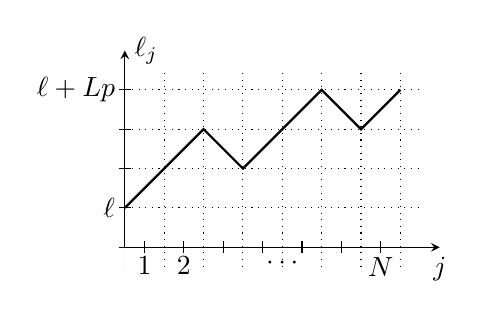
\begin{tikzpicture}[>=stealth]
     \draw[scale=0.5,thick] (0,0)--(2,2)--(3,1)--(5,3)--(6,2)--(7,3);
           
     \draw[<->] (0,2) -- (0,-0.5) -- (4,-0.5);
     \foreach \x in {0.25,0.75,...,3.25}
       \draw[xshift=\x cm,yshift=-0.5cm] (0,-0.075)--(0,0.075);
     
    \foreach \y in {-0.5,0,...,1.5}
       \draw[yshift=\y cm] (-0.075,0)--(0.075,0);
 
    \draw (0.25,-0.5) node[below] {$1$};
    \draw (0.75,-0.5) node[below] {$2$};
    \draw (2,-0.5) node[below] {$\cdots$};
    \draw (3.25,-0.5) node[below] {$N$};
    \draw (4,-0.5) node[below] {$j$};
    \draw (0,0) node [left] {$\ell$};
    \draw (0,1.5) node [left] {$\ell+Lp$};
    \draw (0,2) node [right] {$\ell_j$};
     \clip[scale=0.5] (0,-1.5) rectangle (7.5,3.5);
     \draw[scale=0.5,dotted] (-1,-2) grid (8,5);
  \end{tikzpicture}
\end{tcblisting}
\clearpage


\begin{tcblisting}{colback=blue!5,boxrule=2pt,colframe=blue!75!black,title=Basic Definitions,width=0.75\textwidth}
\newcommand{\ud}{\ensuremath \mathop{}\!\mathrm{d}}
\(z=2\sin x\mathrm{d}x\) and \(z=2\sin x\ud x\)
\end{tcblisting}
\newcommand{\ud}{\mathop{}\!\mathrm{d}}
\bigskip

It uses an empty operator and eliminates the space
on its left with |\!|.

Note the difference between

\[z=2\sin x\mathrm{d}x  \]

\[z=2\sin x\ud x\]

where the diffrential is obtained respectively with
|\mathrm{d}| and |\ud|.




\newthought{God is in the details}

Sometimes you will be faced with small decisions for which the Journal style manual might not have an answer for you or the editor might have a different opinion to yours. One such question is if one needs to insert the thousand separator in coefficients.

\[
\operatorname{erf}^{-1}(z)=\tfrac{1}{2}\sqrt{\pi}\left (z+\frac{\pi}{12}z^3+\frac{7\pi^2}{480}z^5+\frac{127\pi^3}{40320}z^7+\frac{4369\pi^4}{5806080}z^9+\frac{34807\pi^5}{182476800}z^{11}+\cdots\right )
\]


\[
\operatorname{erf}^{-1}(z)=\tfrac{1}{2}\sqrt{\pi}\left (z+\frac{\pi}{12}z^3+\frac{7\pi^2}{480}z^5+\frac{127\pi^3}{40,320}z^7+\frac{4,369\pi^4}{5,806,080}z^9+\frac{34,807\pi^5}{182,476,800}z^{11}+\cdots\right )
\]

\[
\operatorname{erf}^{-1}(z)=\tfrac{1}{2}\sqrt{\pi}\left (z+\frac{\pi}{12}z^3+\frac{7\pi^2}{480}z^5+\frac{127\pi^3}{40{,}320}z^7+\frac{4{,}369\pi^4}{5{,}806{,}080}z^9+\frac{34{,}807\pi^5}{182{,}476,800}z^{11}+\cdots\right )
\]



\[
\operatorname{erf}^{-1}(z)=\tfrac{1}{2}\sqrt{\pi}\left (z+\frac{\pi}{12}z^3+\frac{7\pi^2}{480}z^5+\frac{127\pi^3}{40\thinspace 320}z^7+\frac{4\thinspace 369\pi^4}{5\thinspace 806\thinspace 080}z^9+\frac{34\thinspace 807\pi^5}{182\thinspace 476\thinspace 800}z^{11}+\cdots\right )
\]


It is interesting to note that Knuth believes that in equations this is unecessary.
He is quoted in Typesetting Mathematics.

\begin{quotation}
But where Don wrote 1000000 they substituted
1,000,000. Don objected that although this might be justifed in text, his use is perfectly OK in a formula. Well then, they replied, write \(10^6\).
Fine, said, Don, but what do I do 
when the number is 1234567? The IEEE standard here is to insert spaces, thus: 1 234 567.
Don doesn't like this in formulae, but agrees that it may be useful in a high precision context, such as numerical tables. 
\end{quotation}



The following are extracts from his paper \footnote{\url{http://www-cs-faculty.stanford.edu/~uno/papers/jfsp.tex.gz}}

{
\[\vcenter{\halign{$#$\hfil\ &$#$\hfil\cr
\Sigma n^{11}&=39916800{n+6\choose 12}+
19958400{n+5\choose 10}+3160080{n+4\choose 8}
+168960{n+3\choose 6}\cr
\noalign{\smallskip}
&\qquad\null+2046{n+2\choose 4}+{n+1\choose 2}\,;\cr
\noalign{\smallskip}
\Sigma n^{13}&=6227020800{n+7\choose 14}+3632428800{n+6\choose 12}+
726485760{n+5\choose 10}\cr
\noalign{\smallskip}
&\qquad\null+57657600{n+4\choose 8}
+1561560{n+3\choose 6}+8190{n+2\choose 4}+{n+1\choose 2}\,.\cr}}\]
}

Also, note in the last equation the use of a period at the end. This is something that strong opinions and flaming wars in fora. I am not too sure if I agree on the last one, but the way that Knuth writes is very clear and his equations in a way are paragraphs. In this case the use of a period is recommended.


\newthought{Punctuation}

There are two schools of thought when it comes to punctuation, that is punctuation in display style formulae. Some authors (Beccari,2007 a), others that it is necessary and essential.

The authors of this article believe that formulae,
both in display and text style, are part of the argumentation
and so punctuation should be used to help
the reader. An example of good use of punctuation is:


Since
\[ a=b \]
and
\[b=c,\]
it is proven that
\[a =c. \]



\subsection{Numbering Equations}

One question that you may face is the numbering of display equations. Early books used numbering sparingly, whereas many authors go overboard and number all the equations.

According to Knuth et al:\footnote{\url{http://tex.loria.fr/typographie/mathwriting.pdf}}

Numbering all displayed formulas is usually a bad idea; number the important ones only.
Halmos\footnote{\url{http://www.math.uh.edu/~tomforde/Books/Halmos-How-To-Write.pdf}} offers pretty much the same good advice,

\begin{quotation}
What about "inequality (*)", or "equation (7)", or "formula (iii)"; should all displays be labelled or numbered? My answer is no. Reason: just as you shouldn't mention irrelevant assumptions or name irrelevant concepts, you also shouldn't attach irrelevant labels. Some small part of the reader's attention is attracted to the label, and some small part of his mind will wonder why the label is there. If there is a reason, then the wonder serves a healthy purpose by way of preparation, with no fuss, for a future reference to the same idea; if there is no reason, then the attention and the wonder were wasted.
\end{quotation}

See also discussion at \url{http://tex.stackexchange.com/questions/29267/which-equations-should-be numbered/49080\#49080}

\url{http://tex.stackexchange.com/questions/29267/which-equations-should-be-numbered/49080#49080}

Now if you wish to argue about this is fine.

\section{Mathmode}

TeX is in \textit{mathmode} when it is reading mathematics. The |ifmmode| can be used to find out if TeX is in math mode. It denotes the start of an if-then-else control structure that tests whether \tex is currently in either math mode or display math mode. The |\else| part is optional. <TeX code 1> is processed if TeX is in one of the math modes, otherwise it is ignored. If the |\else| section is included and TeX is not in one of the math modes then <TeX code 2> is processed; otherwise it is ignored.


\begin{texexample}{}{}

\newcommand{\Acal}{\ifmmode \mathcal{Acal} \else \(\mathcal{Acal}\) \fi}
The command efines a macro |\Acal| that can be used both in and out of math mode to typeset a calligraphy script A. 

This is a calligraphic \Acal\ or \(\Acal\).
\end{texexample}


\section{Useful packages}

Besides the main packages that we have discussed so far and which should be in everyone's toolbox, there are a number of other packages that you may find useful. One such package is the |\multienum|, which although not really a packaged specializing in mathematical typesetting, it provides an environment to set multiple equations, as in an exercise or exam.



\subsection{the multienum package}

The \docpkg{multienum} enables  the typestting of multiple equations on one line and numbering them, either with roman, arabic or alpha letters.

\emphasis{usepackage, multienum,begin,end,multienumerate}
\begin{teXXX}
\documentclass{article}
\usepackage{multienum}
\renewcommand{\regularlisti}{\setcounter{multienumi}{0}%
  \renewcommand{\labelenumi}%
  {\addtocounter{multienumi}{1}\alph{multienumi})}}
\begin{document}
\begin{multienumerate}[oddlist]
\mitemxxx{\(x^2 + y^2 = 1\)}{\(a + b = c\)}{\(r-x = y+z\)}
\mitemxxx{\(f - y = z\)}{\(a - b = 2d\)}{\(r+x = 2y-3z\)}
\end{multienumerate}
\end{document}
\end{teXXX}


\begin{multienumerate}[oddlist]
\mitemxxx{\(x^2 + y^2 = 1\)}{\(a + b = c\)}{\(r-x = y+z\)}
\end{multienumerate}
\begin{multienumerate}[evenlist]
\mitemxxx{\(f - y = z\)}{\(a - b = 2d\)}{\(r+x = 2y-3z\)}
\end{multienumerate}


\hrule

\bigskip

We can also enumerate the items using an even-only or odd only
counter.
\subsection*{Answers to Even-Numbered Exercises}
\begin{multienumerate}[evenlist]
\mitemxxxx{Not}{Linear}{Not}{Quadratic}
\mitemxxxo{Not}{Linear}{No; if $x=3$, then $y=-2$.}
\mitemxx{$(x_1,x_2)=(2+\frac{1}{3}t,t)$ or
$(s,3s-6)$}{$(x_1,x_2,x_3)=(2+\frac{5}{2}s-3t,s,t)$}
\mitemx{$(x_1,x_2,x_3,x_4)= (\frac{1}{4}+\frac{5}{4}s+\frac{3}{4}t-u,s,t,u)$
or $(s,t,u,\frac{1}{4}-s+\frac{5}{4}t+\frac{3}{4}u)$}
\mitemxxxx{$(2,-1,3)$}{None}{$(2,1,0,1)$}{$(0,0,0,0)$}
\end{multienumerate}
\bigskip



\newcommand\thecasestudylabel{Case Study}
\newenvironment{casestudy}[2][]{%
   \clearpage\par\leavevmode
   \addcontentsline{toc}{section}{\thecasestudylabel:  #1}
    \topline\vskip1.5pt
   {\noindent\large CASE STUDY\par}\vspace{3.5pt}
   \noindent\textsc{\large#1}\par
   \bigskip
   {#2}
   \medskip
   \topline
}{%
\vfill\bottomline}

\begin{casestudy}[The Riemann hypothesis.]{%
Typeset the text and the equations, shown below. Use a standard minimal to achieve it. Note the fraktur fonts. Text must all be as one paragraph.}

It is well known that the Riemann zeta function $\zeta(s)$ of a complex variable $s=\sigma+it$ is defined by
\[
\zeta(s)=\sum_{n=1}^{\infty}\frac{1}{n^{s}}
\]
for the real part $\mathfrak{R}(s)>1$ and its analytic continuation in the half plane $\sigma>0$ is
\begin{equation}\label{func:zeta}
\zeta(s)=\sum_{n=1}^{N}\frac{1}{n^{s}}-\frac{N^{1-s}}{1-s}-\frac{1}{2}N^{-s}
+s\int_{N}^{\infty}\frac{\frac{1}{2}-\{x\}}{x^{s+1}}dx
\end{equation}
for any integer $N\geq1$ and $\mathfrak{R}(s)>0$.
It extends to an analytic function in the whole complex plane except for having a simple pole at $s=1$. Trivially, $\zeta(-2n)=0$ for all positive integers. All other zeros of the Riemann zeta functions are called its nontrivial zeros.
\bottomline

\begin{teX}
It is well known that the Riemann zeta function $\zeta(s)$ of a complex variable $s=\sigma+it$ is defined by
\[
\zeta(s)=\sum_{n=1}^{\infty}\frac{1}{n^{s}}
\]
for the real part $\mathfrak{R}(s)>1$ and its analytic continuation in the half plane $\sigma>0$ is
\begin{equation}\label{func:zeta}
\zeta(s)=\sum_{n=1}^{N}\frac{1}{n^{s}}-\frac{N^{1-s}}{1-s}-\frac{1}{2}N^{-s}
+s\int_{N}^{\infty}\frac{\frac{1}{2}-\{x\}}{x^{s+1}}dx
\end{equation}
for any integer $N\geq1$ and $\mathfrak{R}(s)>0$.
It extends to an analytic function in the whole complex plane except for having a simple pole at $s=1$. Trivially, $\zeta(-2n)=0$ for all positive integers. All other zeros of the Riemann zeta functions are called its nontrivial zeros.
\end{teX}

Please note that the maths and the text, are typed as a single block. Do not leave any spaces in between. We have used |\mathfrak| for the fraktur font. We have also used $it$ for the imaginary part. This would depend on the style used in your field. 
\end{casestudy}

\clearpage
\section{Gather}
This is like a multi line environment with no special horizontal alignment. All rows
are centered and can have an own equation number:

\begin{tcblisting}{colback=blue!5,boxrule=2pt,colframe=blue!75!black,title=The gather environment,width=\textwidth,before=\bigskip,after=\bigskip}
\def\O{\mathcal{O}}
\begin{gather}
 \O,\O(E_4),\O(E_2),\O(H-E_3-E_5),\O(H-E_3),\O(H-E_5),\\ 
\O(2H-E_1-E_3-E_5-E_6),\O(2H-E_1-E_3-E_5),\O(2H-E_3-E_5-E_6).
\end{gather}

So lautet der Beweis des Satzes $2 \times 2 = 4$:
\begin{gather}
(\Omega^{\nu})^{\mu}{}'x = \Omega^{\nu \times \mu}{}'x \text{ Def.}\\
%\begin{split}
\Omega^{2 \times 2}{}'x = (\Omega^{2})^{2}{}'x = (\Omega^{2})^{1 + 1}{}'x = \Omega^{2}{}'\Omega^{2}{}'x = \Omega^{1 + 1}{}'\Omega^{1 + 1}{}'x\nonumber \\
= (\Omega'\Omega)'(\Omega'\Omega)'x = \Omega'\Omega'\Omega'\Omega'x = \Omega^{1 + 1 + 1 + 1}{}'x = \Omega^{4}{}'x.
%\end{split}
\end{gather}


\begin{gather*}
x = \Omega^{0}{}' x \text{ Def.\ and}\\
\Omega'\Omega^{\nu}{}'x = \Omega^{\nu+1}{}'x \text{ Def.}
\end{gather*}
\begin{equation}
x = \Omega^{0}{}' x \text{ Def.\ and}\\
\Omega'\Omega^{\nu}{}'x = \Omega^{\nu+1}{}'x \text{ Def.}
\end{equation}
\end{tcblisting}






%  \makeatletter
\newcommand\QEDit{\hspace{6pt}\textit{Q.~E.~D.}\quad}
\newcommand\QEFit{\hspace{6pt}\textit{Q.~E.~F.}\quad}
\newcommand\QEIit{\hspace{6pt}\textit{Q.~E.~I.}\quad}
\newcommand\QEDup{\hspace{6pt}Q.~E.~D.\quad}
\newcommand\QEFup{\hspace{6pt}Q.~E.~F.\quad}
\newcommand\QEIup{\hspace{6pt}Q.~E.~I.\quad}
\newcommand\QEOup{\hspace{6pt}Q.~E.~O.\quad}
\newcounter{wrapwidth}
\newcount \Zw
\newcount \Zh


\newcommand\pngright[4]{%
    \Zw=#2 \divide \Zw by 10
    \Zh=#3 \divide \Zh by 120  \advance\Zh by 1
    \setcounter{wrapwidth}{\Zw}
\begin{wrapfigure}[\Zh]{r}{\value{wrapwidth}pt}%
\begin{center}
\vspace{#4pt}%
\includegraphics*[width=\Zw pt]{images/#1}%
\end{center}
\end{wrapfigure}}

\newcommand\propnopage[1]{
\begin{center}{\large #1}\end{center}}

\parindent1em

\cxset{toc image=\@empty}
\chapter{PERICULA}

\noindent\textsc{Case Study: } We will now typeset a section, from Isaac Newton's \textit{Philosophi\ae\  Naturalis Principia Mathematica}. The typeset example is shown below.

\bottomline
\bgroup
\small

\cxset{section align=center,
         section numbering=none}

\section{{SECT}$\cdot$ VIII$\cdot$}

\begin{center}{\textit{De Motu per Fluida propagato.}}\end{center}

\makeatletter
%\propnopage{Prop.\ XLI\@. Theor.\ XXXI.}
\meaning\@
\makeatother

\textit{Pressio non propagatur per Fluidum secundum lineas rectas, nisi
ubi particul{\ae} Fluidi in directum jacent.}

Si jaceant particul{\ae} $a$, $b$, $c$, $d$, $e$ in linea recta, potest quidem
pressio directe

\begin{wrapfigure}[8]{O}[1pt]{0.3\textwidth}
  \vspace{-17pt}
  \includegraphics[width=0.27\textwidth]{images/362.png}
\end{wrapfigure}

\noindent propagari  ab $a$ ad $e$; at
particula $e$ urgebit particulas oblique positas
$f$ \& $g$ oblique, \& particul{\ae} ill{\ae} $f$ \& $g$
non sustinebunt pressionem illatam, nisi fulciantur
a particulis ulterioribus $h$ \& $k$;
quatenus autem fulciuntur, premunt particulas
fulcientes; \& h{\ae} non sustinebunt pressionem nisi fulciantur
ab ulterioribus $l$ \& $m$ easque premant, \& sic deinceps in infinitum.
Pressio igitur, quam primum propagatur ad particulas
qu{\ae} non in directum jacent, divaricare incipiet \& oblique propagabitur
in infinitum; \& postquam incipit oblique propagari, si
inciderit in particulas ulteriores, qu{\ae} non in directum jacent, iterum
divaricabit; idque toties, quoties in particulas non accurate
in directum jacentes inciderit. \QEDit

\topline

\vspace*{-\baselineskip}
\captionof{figure}{Example of a typeset page from Principi\ae.}
\egroup
\smallskip
Figure~\ref{fig:principia}, shows a scan of the actual page. We will not reproduce, the fonts and the page geometry exactly, but rather we will attempt to extract and reproduce the typographical rules employed in the printing of the \textit{Principi\ae}.

We begin by typesetting the section number and its heading. The use of roman numbers creates better harmony between the text and the heading

\begin{teX}
\sectpage{VIII$\middot$}
\begin{center}{\textit{De Motu per Fluida propagato.}}\end{center}
\end{teX}
The proposition and theorem line, has its own command
\begin{teX}
\makeatletter
\propnopage{Prop.\ XLI. Theor.\ XXXI.}
\makeatother
\end{teX}

\propnopage{\color{gray}Prop.\ XLI\@. Theor.\ XXXI.}
\vspace*{-37pt}
\propnopage{Prop. XLI. Theor. XXXI.}


Notice the small differences in the spacing with the commands as shown and with the black text, without them. The rest is based on normal \LaTeX\ commands.

\textit{Pressio non propagatur \ldots particul{\ae}\ldots}

\pngright{362.png}{709}{603}{-24}

Si jaceant particul{\ae} $a$, $b$, $c$, $d$,
$e$ in linea recta, potest quidem
pressio directe propagari ab $a$ ad $e$; at


Remember that it is important to start a new paragraph after the 
|pngright| command. The |wrapfig| package works by using |everypar| to insert the hanging indentation.

\begin{figure}[p]
\centering
\includegraphics[scale=1]{./images/page354.png}
\caption{Page 354 from Isaac Newton's \textit{Philosophi\ae\  Naturalis Principia Mathematica}. Image was obtained from Google's copy, available at Google Books.}
\label{fig:principia}
\end{figure}
\makeatother

%  \chapter{Italics}

\index{Petrarch}
The first Italic type letter was derived, it is said, from the handwriting of Petrarch, and several admirable examples of the style, variously treated, have come down to us. As far as construction goes Italic is, theoretically, only the exact Roman form sloped, and with such changes as are necessitated by the sloping of the letters. Practically, however, it will be found that certain alterations in the outlines of the Roman letters must be made after giving them a slope in order to adapt them to their new requirements of inter-juxtaposition; and, by a reflex action, when words in Italic capitals are used in the same panel with upright Roman letters, certain variations must be made in the latter, such as accenting the Roman O in the same fashion as the Italic O is accented, an altered treatment of serifs, and other changes in detail.

\section{Typesetting italic text}
In \LaTeX\ three commands can be used to produce italic text: \verb+\textit, \emph+ and  \verb+\tt+. These are used as shown below:


\begin{verbatim}
The speaker is, \textit{ex officio}, the chairman.
The speaker is, \emph{ex officio}, the chairman.
The speaker is, {\tt ex officio}, the chairman.
\end{verbatim}

These will produce identical text as shown below,
\smallskip

\qquad  The speaker is, \textit{ex officio}, the chairman.

\qquad The speaker is, \emph{ex officio}, the chairman.

\qquad The speaker is, {\it ex officio}, the chairman.
\smallskip

The last one is the original \TeX\ command, but it is generally frowned upon to use it with \LaTeX\ despite the fact that Lamport has redefined it to be equaivalent to \verb+\textit+. Note that the last one needs to be enclosed in
braces unless you want your text from that point onwards to be typeset in italic font.

When typesetting mathematics, the \TeX\ engine typeset using italics unless specifically instructed to do otherwise:

\[\underbrace{\overbrace{a+b+c}^6
\cdot \overbrace{d+e+f}^9}
_\text{meaning of life} = 42\]

\begin{figure}
\includegraphics[width=0.8\textwidth]{petrarch}
\caption{Original lyrics by Petrarch, found in 1985 in Erfurt (source Wikipedia)}
\end{figure}

\chapter{RULES FOR THE USE OF ITALIC}

One very important principle should always be observed in the use of italic for emphasis. Emphasis should always be used sparingly. Make the words do their work. Do not try to supplement poverty of thought and weakness of expression by italics, capitals, and other marks of emphasis. Where there is too much emphasis attempted no emphasis is secured. This fault was much more common formerly than now.

The accompanying reproduction of a page from a book printed in 1690 (place not given, but probably London) illustrates several of the faulty uses of italics common at that time. An entire paragraph is italicized (quite unnecessarily) for emphasis. All proper names and adjectives derived from them are italicized where they occur in the regular text and printed in roman where they occur in italicized passages. Note the frequent capitalization for emphasis and especially the italic capital with roman lower-case in the first line of the second paragraph. This is a frequent usage in this particular book. In this book all quotations are printed in italic without quote marks. The paper, composition, and presswork of the book are very poor. It represents English printing in its worst period.

Moderation in the use of italics is so important that in many cases the compositor is justified in ignoring markings for italic in his copy where they are too profuse. The author is often surprised and disappointed at the appearance[7] of his proof when it comes back heavily italicized. Moreover the occurrence of many italics increases the cost of composition because of the greater labor involved.

\begin{enumerate}
\item  Italicize, subject to the caution just given, any words or phrases which it is desired to emphasize.

\item Foreign words and phrases incorporated into English sentences are sometimes italicized and sometimes not so distinguished. The deciding element in fixing the usage in these cases would seem to be the commonness and familiarity of the word or phrase. For example, the meaning of bona fide (Latin), menu (French), recto (Italian), or stein (German) are as well known as those of most English words. To all intents and purposes these words have been adopted into our language. On the other hand, jeu d'esprit (French) or inter alia (Latin) would probably not be immediately understood by the casual reader. Words of the first type should not be italicized. Words of the second type should be.

\item Do not italicize foreign titles preceding names of foreign institutions or places, streets, etc., the meaning or position of which in English would call for roman type.
        \begin{quote}
         \noindent Pere Ladeau; Freiherr von Schwenau; the Place de la Concorde; the Museo delle Terme.
       \end{quote}

\item In text matter use roman for the name of any author, but italicize the title of the work. This applies to books, including plays, essays, cycles of poems, and single poems of considerable length, usually printed separately, and not from the context understood to form parts of a larger volume; pamphlets, treatises, tracts, documents, and periodicals (including regularly appearing proceedings and transactions). In the case of newspapers and periodicals the [10] name of the place of publication should be italicized when it forms an integral part of the name, but do not under ordinary circumstances italicize the article \emph{the}.


\item The phrases \textit{prima facie} and \textit{ex officio} are sometimes used to qualify the nouns which follow, and sometimes used as adverbs. As qualifiers they are often printed in roman with the hyphen.

     \hspace*{1em} Prima-facie evidence.

     \hspace*{1em} An ex-officio member of all committees.


When used as adverbs they may be printed in italics without the hyphen.

\qquad The evidence is, \textit{prima facie}, convincing.

\qquad The speaker is, \textit{ex officio}, the chairman.

Names of ships, especially when they are taken from places, as in the United States Navy, are often italicized.

\qquad\qquad U.S.S. \textit{Philadelphia}, U.S.S. \textit{Alabama}.

\item  Italicize particular letters of the alphabet when referred to as such.

         We use \emph{a} much more frequently than \emph{q}.
\end{enumerate}



\subsubsection{The italic correction}

\begin{figure}[htbp]
\vspace*{1ex}
\centering
\fbox{\begin{minipage}{0.28\textwidth}
\rmfamily

{\noindent{\scalebox{3}{\color{gray!70}(fjordtl)}}}

\fbox{{{\scalebox{3}{\color{red}\textit{(fjordtl\/)}}}}}

\fbox{{{\scalebox{3}{\color{red}\textit{(fjordtl)}}}}}

{{\scalebox{3}{\color{red}$(fjordtl)$}}}
\end{minipage}}

\caption{Italic correction}
\end{figure}

%  \makeatletter\@specialfalse

\cxset{
 toc image = \@empty,
 name={},
 numbering=arabic,
 number font-size= LARGE,
 number font-family= rmfamily,
 number font-weight= bfseries,
 number before=,
 number dot=,
 number after=,
 number position=leftname,
 chapter font-family= sffamily,
 chapter font-weight= normalfont,
 chapter font-size= Large,
 chapter before={\vspace*{15pt}\par},
 chapter after={\hfill\hfill\par},
 number color=black!90,
 title beforeskip={\vspace*{30pt}},
 title afterskip={\vspace*{40pt}\par},
 title before={},
 title after={},
 title font-family= sffamily,
 title font-color= black,
 title font-weight= bfseries,
 title font-size= LARGE,
 header style= plain,
 }

\cxset{headings ruled-01}

\chapter{Introduction to Style One}


\begin{summary}
This design is simple and its distinguishing characteristic is a short summary at the beginning of the chapter. This is almost like an abstract typeset in italic font without setting the margins in. We provide a \lstinline{summary} environment for convenience. Note the very simple line in the running head to the left of the page number.
\end{summary}

\medskip
\begin{figure}[ht]
\centering
\includegraphics[width=0.5\textwidth]{./chapters/chapter01.png}
\end{figure}
\makeatother

%  \makeatletter
%  \cxset{toc image=false},

\long\gdef\versochapter#1{%
  \vspace*{3cm}
  \minipage{\textwidth}
  \hfill\includegraphics[width=0.63\textwidth]{\chapterimage@cx}\par
  \vspace*{6pt}
  \hfill\minipage{0.75\textwidth}
  {\HUGE\bfseries\flushright #1\endflushright}
  \endminipage
  \endminipage
  \newpage


\vspace*{10cm}
\@specialfalse
\@openleftfalse
\@openanyfalse
\@openrighttrue
}


\newgeometry{bottom=2.5cm}

\cxset{
   chapter image/.code={\def\chapterimage@cx{#1}},
   chapter opening/.is choice,
   chapter opening/verso/.code={\@specialtrue\@openlefttrue
   \gdef\customdesign@cx##1{\versochapter{##1}}}
}

\cxset{
 chapter image=onesowndeath,
 chapter opening=verso,
 name={},
 numbering=none,
 number font-size=\LARGE,
 number font-family=\rmfamily,
 number font-weight=\bfseries,
 number before=,
 number dot=,
 number after=,
 number position=leftname,
 chapter font-family=\sffamily,
 chapter font-weight=\normalfont,
 chapter font-size=\Large,
 chapter before={\vspace*{0pt}\par},
 chapter after={\hfill\hfill\par},
 chapter color={black!90},
 number color=\color{purple},
 title beforeskip={\vspace*{0pt}},
 title afterskip={\vspace*{0.4\textheight}\par},
 title before={},
 title after={},
 title font-family=\sffamily,
 title font-color=\color{purple},
 title font-weight=\bfseries,
 title font-size=\LARGE,
 header style=plain,
 pagestyle=plain,
 }

\@specialtrue

\chapter[VERSO CHAPTERS]{Verso Chapters}

\parindent1.5em
{\HUGE V}erso chapter openings are not common. One design that I found quite attractive is \lipsum[1-3] \textit{From Western attitudes toward death from the middle ages to the present}, Philippe Ari\'es. London, 1974.

\begin{figure}
\includegraphics[width=\textwidth]{versochapter01}
\caption{Chapter opening on verso page.}
\end{figure}


% \makeatletter
% \newgeometry{top=-10pt,bottom=2cm}


\cxset{style03/.style={
 toc image = \@empty,
 name={},
 numbering=arabic,
 number font-size= HUGE,
 number font-family= rmfamily,
 number font-weight= bfseries,
 number before=\par\vspace*{10pt}\hfill\hfill,
 number dot=.,
 number after=,
 number position=rightname,
 chapter font-family= sffamily,
 chapter font-weight=normalfont,
 chapter font-size= Large,
 chapter before={\hspace*{-2.5cm}\vbox\bgroup%
    \tcbset{width=\paperwidth,boxrule=0pt,right=3cm,arc=0pt}
    \tcolorbox\bgroup\vspace*{20pt}\hfill\hfill},
 chapter after={\par\vspace*{15pt}},
 chapter color=black!90,
 number color= thered,
 title beforeskip={},
 title afterskip={\vspace*{10pt}\par},
 title before={\hfill\hfill},
 title after={\vspace*{60pt}\egroup\endtcolorbox\egroup},
 title font-family=\sffamily,
 title font-color= thered,
 title font-weight=\bfseries\RaggedRight,
 title font-size=\Huge}}

\cxset{style03}

\chapter{Introduction Style Three}

This is not an exact reproduction as I am still thinking as to how to use
specials with the package. You can vary it by setting the tcolorbox settings as well as the geometry settings.
\medskip

\begin{figure}[ht]
\centering
\includegraphics[width=0.39\textwidth]{./chapters/chapter03}
\end{figure}

This setting involves changing the geometry of the page as well as adding the chapter name and title in a color box. For this I have used the \lstinline{tcolorbox}. Of course you can use any other shaded environment you feel comfortable with such as mdframed. It is important to set the colorbox parameters.

\begin{lstlisting}
\newgeometry{top=-10pt}
\tcbset{width=\paperwidth,boxrule=0pt,right=3cm,arc=0pt}
\end{lstlisting}

Note that we set the width of the \lstinline{tcolorbox} to \lstinline{\paperwidth} in order for the shading to extend to the full width of the page.

\restoregeometry

% \cxset{style04/.style={
 chapter name=,
 numbering=Roman,
 number font-size=Large,
 number font-family=rmfamily,
 number font-weight=bfseries,
 number before=,
 number dot=,
 number after=,
 number color=black,
 number position=rightname,
 chapter font-family= rmfamily,
 chapter font-weight=bold,
 chapter font-size=Large,
 chapter before=,
 chapter after=,
 chapter color=black!90,
 chapter border-style=none,
 chapter border-width=0pt,
 chapter display=block,
 chapter float=center,
 title beforeskip={},
% title afterskip={\vspace*{50pt}\par},
 title margin bottom=50pt,
 title margin-left=0pt,
 chapter title align=centering,
 chapter title text-align=center,
 chapter title width=\textwidth,
 title display=block,
 title border-left-width=0.2pt,
% title hooks leave emptt 
 title before=,
 title after=,
 % title families leave as default font name
 title font-family=rmfamily,
  title font-color= black,
 title font-weight=normalfont,
 title font-size=LARGE,
 % title alignment
 chapter title align=centering,
 % sectioning incomplete please add to suit
 section numbering=none,
 section align = center}}

\debugchapter
\cxset{chapter border-width=2pt,
          chapter padding=5pt,
          number border-width=2pt,
          number padding=5pt}

\cxset{style04}

\chapter{INTRODUCTION TO STYLE FOUR}

This is a very simple design applicable perhaps to translations and commentary on older texts.
\medskip
\begin{figure}[ht]
\centering
\includegraphics[width=0.6\textwidth]{./chapters/chapter04.png}
\end{figure}

\testsections



% %%%%%%%%%%%%%%%%%%%%%%%%%%%%%%%%%%%%%%%%%%%
%%%%%%  STYLE 05
%%%%%%%%%%%%%%%%%%%%%%%%%%%%%%%%%%%%%%%%%%%


\cxset{style05/.style={
 name={Chapter},
 numbering=arabic,
 number font-size=\Large,
 number font-family=\rmfamily,
 number font-weight=\normalfont\itshape,
 number color=\color{black!90},
 number before=,
 number dot=,
 number after=,
 number position=rightname,
 chapter font-family=\rmfamily,
 chapter font-weight=\normalfont\itshape,
 chapter font-size=\Large,
 chapter before={\hrule width \columnwidth \kern2.6pt \par\hfill},
 chapter after={\hfill\hfill\par},
 chapter color={black!90},
 chapter spaceout=none,
 title beforeskip={\vspace*{10pt}},
 title afterskip={\vspace*{50pt}\par},
 title before={\hfill},
 title after={\hfill\hfill \vskip2.6pt\hrule width \columnwidth \kern2.6pt },
 title font-family=\rmfamily,
 title font-color=\color{black!90},
 title font-weight=\bfseries,
 title font-size=\huge,
 header style= headings}}

\cxset{style05}
\chapter{Introduction to Style Five}\index{ch:style5}

\tcbset{width=\textwidth}
I think this style can be improved with a bit of color. You can experiment with it quite easily. The spacing on top of this style can also be adjusted to suit your typographical taste.
\medskip
\begin{figure}[ht]
\centering
\includegraphics[width=0.6\textwidth]{./chapters/chapter05}
\end{figure}

%\section{General notes on rules}

LaTeX's default rules would normally give problems. Best is to use TeX's primitives to built them.

%\index{rules!example color}
%\begin{texexample}{}{}
%\makeatletter
%\hrule width 5cm \kern2.6\p@
%AAAAAAAAAAAAAAAAAAAAA
%\vskip2.6pt\hrule width 5cm
%\medskip
%
%Problem with LaTeX rules.
%
%\rule{5cm}{0.4pt}\par
%AAAAAAAAAAAAAAAAAAAAA\par%
%\rule[6.5pt]{5cm}{0.4pt}
%
%\def\rule{\@ifnextchar[\@rule{\@rule[\z@]}}
%\def\@rule[#1]#2#3{%
% \leavevmode
% \hbox{%
% \setlength\@tempdima{#1}%
% \setlength\@tempdimb{#2}%
% \setlength\@tempdimc{#3}%
% \advance\@tempdimc\@tempdima%
% \vrule\@width\@tempdimb\@height\@tempdimc\@depth-\@tempdima}}
%
%\def\thickrule{\leavevmode \leaders \hrule height 3pt \hfill \kern \z@}
%
%{\color{teal}\hrule width 10.5cm height3pt \kern2.6\p@
%    {{\color{black!80}\HUGE CHAPTER TITLE}}\vskip3pt
%\hrule width 10.5cm height3pt}
%\makeatother
%\end{texexample}

% <<<<<<< HEAD
%%%%%%%%%%%%%%%%%%%%%%%%%%%%%%%%%%%%%%%%%%%
%%%%%%  STYLE 06
%%%%%%%%%%%%%%%%%%%%%%%%%%%%%%%%%%%%%%%%%%%

\cxset{style06/.style={
 name={Chapter},
 numbering=arabic,
 number font-size=\Huge,
 number font-family=\calligra,
 number font-weight=\calligra,
 number color=\color{black!90},
 number before=\kern-2.5pt,
 number dot=,
 number after=,
 number position=rightname,
 chapter font-family=\rmfamily,
 chapter font-weight=\calligra,
 chapter font-size=\LARGE\calligra,
 chapter before={\vspace*{20pt}\par\hfill},
 chapter after={\hfill\hfill\par},
 chapter color={black!90},
 title beforeskip={\vspace*{50pt}},
 title afterskip={\vspace{3.5pt}\par},
 title before={\hfill},
 title after={\hfill\hfill},
 title font-family=\rmfamily,
 title font-color=\color{black!90},
 title font-weight=\normalfont,
 title font-size=\LARGE,
 title spaceout=soul,
}}

\cxset{style06}

\chapter{INTRODUCTION TO STYLE SIX}
\renewcommand{\DefaultLhang}{0.1}
\renewcommand{\LettrineFontHook}{\calligra}
\setlength{\DefaultFindent}{9.5pt}
\setlength{\DefaultNindent}{0pt}

\lettrine{\textcolor{orange}{T}}{}he calligraphic font for this design make it stand out, although you may need to experiment to get the right font (I have used calligra). I am sure the specification can be optimized a bit, however so far it works. I also opted to space out the title. I had to experiment a bit to get the Lettrine settings.
\medskip
\begin{figure}[ht]
\centering
\includegraphics[width=0.6\textwidth]{./chapters/chapter06}
\end{figure}

The number has been kerned using:

\begin{lstlisting}
 number before=\kern-4.5pt,
\end{lstlisting}

This template has a lot of potential and I will come back to it and add more key hooks for lettrine settings per letter and font management. They can also come alive with a gold color.

=======
%%%%%%%%%%%%%%%%%%%%%%%%%%%%%%%%%%%%%%%%%%%
%%%%%%  STYLE 06
%%%%%%%%%%%%%%%%%%%%%%%%%%%%%%%%%%%%%%%%%%%

\cxset{style06/.style={
 name={Chapter},
 numbering=arabic,
 number font-size=\Huge,
 number font-family=\calligra,
 number font-weight=\calligra,
 number color=\color{black!90},
 number before=\kern-2.5pt,
 number dot=,
 number after=,
 number position=rightname,
 chapter font-family=\rmfamily,
 chapter font-weight=\calligra,
 chapter font-size=\LARGE\calligra,
 chapter before={\vspace*{20pt}\par\hfill},
 chapter after={\hfill\hfill\par},
 chapter color={black!90},
 title beforeskip={\vspace*{50pt}},
 title afterskip={\vspace{3.5pt}\par},
 title before={\hfill},
 title after={\hfill\hfill},
 title font-family=\rmfamily,
 title font-color=\color{black!90},
 title font-weight=\normalfont,
 title font-size=\LARGE,
 title spaceout=soul,
}}

\cxset{style06}

\chapter{INTRODUCTION TO STYLE SIX}
\renewcommand{\DefaultLhang}{0.1}
\renewcommand{\LettrineFontHook}{\calligra}
\setlength{\DefaultFindent}{9.5pt}
\setlength{\DefaultNindent}{0pt}

\lettrine{\textcolor{orange}{T}}{}he calligraphic font for this design make it stand out, although you may need to experiment to get the right font (I have used calligra). I am sure the specification can be optimized a bit, however so far it works. I also opted to space out the title. I had to experiment a bit to get the Lettrine settings.
\medskip
\begin{figure}[ht]
\centering
\includegraphics[width=0.6\textwidth]{./chapters/chapter06}
\end{figure}

The number has been kerned using:

\begin{lstlisting}
 number before=\kern-4.5pt,
\end{lstlisting}

This template has a lot of potential and I will come back to it and add more key hooks for lettrine settings per letter and font management. They can also come alive with a gold color.

>>>>>>> merged

% 
\newgeometry{top=2cm,bottom=2cm,left=3cm,right=3cm}

\setdefaults

\cxset{style07/.style={
 name={},
 chapter toc=true,
 numbering=arabic,
 number font-size=HUGE,
 number font-family=sffamily,
 number font-weight=bfseries,
 number before=,
 number dot=,
 number color= gray,
 number after=\par,
 number position=leftname,
 chapter font-family=\sffamily,
 chapter font-weight=\normalfont,
 chapter font-size=\Large,
 chapter before={\hfill\hfill\hfill\par},
 chapter after={\vspace*{20pt}},
 chapter color= black!90,
 title beforeskip={\vspace*{30pt}},
 title afterskip={\vspace*{50pt}\par},
 title before={},
 title after={\par\rule[17pt]{\textwidth}{0.4pt}},
 title font-family=\sffamily,
 title font-weight=\bfseries,
 title font-size=\LARGE,
 title font-shape=normal,
 title font-color=black!90,
 title spaceout=none,
}}

\cxset{style07}
\chapter{Introduction to Style Seven}

\parindent0pt
\lipsum[1]
\medskip
\begin{figure}[ht]
\centering
\includegraphics[width=0.6\textwidth]{./chapters/chapter07.png}
\end{figure}
\lipsum[1]

% \clearpage

\setdefaults

\makeatletter
\cxset{style08/.style={
 name={},
 chapter toc=true,
 numbering=arabic,
 number font-size=\LARGE,
 number font-family=\sffamily,
 number font-weight=\bfseries,
 number color= black!90,
 number before=,
 number dot=,
 number after=,
 number position=rightname,
 chapter font-family=sffamily,
 chapter font-weight=normalfont,
 chapter spaceout=none,
 chapter font-size=Large,
 chapter before=,
 chapter after=,
 chapter color={black!90},
 chapter float=right,
 chapter display=block,
 chapter border-style=none,
 chapter border-width=0pt,
 number spaceout=none,
 number display=block,
 number float=right,
 chapter title width=0.6\textwidth,
 title beforeskip=,
 title afterskip=,
 title before=,
 title after={},
 title font-family=sffamily,
 title font-color=black!90,
 title font-weight=bfseries,
 title font-size=LARGE,
 title display=block,
 chapter title align=right,
 author block=true,
 author block format=\par\addvspace{12pt}\normalfont\large\raggedleft,
 author names=Yiannis Lazarides\par Larnaka,
 section number after=,
 section numbering = arabic,
 section numbering prefix=,
 section numbering custom = \@arabic\c@section.\space,
 section color=black,
 section numbering suffix=,
 header style=empty}}
 
 % humanized name of the style, with a non human connotation!
 %
 \cxset{humanoid/.style={style08}}
\makeatother

\cxset{section color=sweet,
          section font-shape=sffamily}


\cxset{style08}
% set the counter needs this to be modified to be based on a key value interface
\cxset{figure numbering/.is choice,
          figure numbering/within/.code=\counterwithin{figure}{chapter},
          figure numbering/without/.code=\counterwithout{figure}{chapter}}
\cxset{table numbering/.is choice,
          table numbering/within/.code=\counterwithin{table}{chapter},
          table numbering/without/.code=\counterwithout{table}{chapter}}          
%\counterwithout{figure}{chapter}

\cxset{figure numbering=without,
          table numbering=without}

\captionsetup[figure]{format = plain,    
                                 width=.67\textwidth,
                                 justification=justified,
                                 singlelinecheck=false,
                                 name=Fig.,
                                 labelsep=period,
                                 oneside,
                                 margin=0pt,
                                 font={normalsize,up}
                                 }
\captionsetup[table]{format = plain,    
                                 justification=justified,
                                 singlelinecheck=false,
                                 labelsep=period,
                                 oneside,
                                 margin=0pt,
                                 labelfont={up,it,normalfont}
                                 }
\chapter[Style 08]{Introduction to Book Style Eight Some Old Fashioned Stops}
\label{st:eight}
\section{Introduction}

This style is suited for Academic publishing, where editors are still a bit old fashioned and require that stops are placed after section numbers, but they do not require that the first line of paragraphs are indented. Any way the good folks that published this book, knew their Affective Computing well and amongst belly dancing  robots and smiling and angry faces, typography can take second place.\footnote{Jimmy Or (\textit{editor}). Affective Computing
Focus on Emotion Expression,
Synthesis and Recognition, May 2008.
}

\example 
\medskip
\begin{figure}[ht]
\centering
\includegraphics[width=0.5\textwidth]{./chapters/chapter08.png}
\caption{The opening page of a chapter in \textit{Affecting Computing}.}
\end{figure}

\solution To add the dot after the number can be done either using the key
\begin{verbatim}
\cxset{section numbering custom = \@arabic\c@section.,}
\end{verbatim}
or by using the pre-built key
\begin{verbatim}
\cxset{section number after=.}
\end{verbatim}

The author block including the institution are added as part of the chapter head styling command.

\example The subject of having articles together in a publication such as Proceedings and Journals is a recurring theme in many Academic fields. One of course if it is possible would have liked to use a standard Journal class and automatically produce this type of publication. There are a number of such classes at \href{http://ctan.org/tex-archive/macros/latex/required/amslatex/amscls/doc/instr-l.pdf}{ctan}

\solution If you are the editor with the task of assembling all these different articles consider using the \pkgname{confproc}. The package by Vincent Verfaille assembles the proceedings from the pdfs, using the 
\pkgname{pdfpages}, which is another great way to achieve this. A simpler way is to develop a specific style for
your Conference and let the participants use it while writing their papers. Only caveat they need to import the
body of the paper with \string\input\meta{article name}. As the \pkgname{phd} comes pre-packaged with
numerous packages the chance of someone using a package that the editor or the system needs to use it
is minimized. Indexing, bibliographies and the like might need to be taken care of and this is discussed in the relevant chapters. There are many options and peculiarities that might not be covered by the phd package so my suggestion is to try it on a few older papers first.

\example  Style-08 has to set the caption style to include for a period after the label number as shown in the Fig.~\ref{fig:eight02}. This can be achieved through key settings or a package.
\begin{figure}[ht]
\centering
\includegraphics[width=\textwidth]{./images/affective-computing.jpg}
\caption{Figures are centered, with the caption flush left and the \textit{Figure} label abbreviated to Fig. (with a stop). The section number also has the dot and follows the style of the sections.}
\label{fig:eight02}
\end{figure}

The figures numbers are reset at every chapter. Normally authors use the \pkgname{chngctr} to achieve such changes, which involves two modifications. Redefining whether or not the figure counter will be reset whenever the chapter/section counter is incremented; Redefining the "appearance" of the figure counter (\string\thefigure), i.e., removing (or adding) the chapter/section prefix.


The standard solution – which deals with modifications 1 and 2 mentioned above – is to use the \string\counterwithout and \string\counterwithin macros of the \texttt{chngcntr package}.\footnote{\protect\url{http://tex.stackexchange.com/questions/28333/continuous-v-per-chapter-section-numbering-of-figures-tables-and-other-docume}} 


\section{Tables}

The Tables follow the style for figures as far as captioning. They are all framed and although there is a genuine distain in the \latexe community for this type of style, I must admit that they are blending well with the style of this book. Another typographical tradition that has been broken in this book is that the table captions are placed below the table and not above.

\example
\begin{figure}[ht]
\centering
\includegraphics[width=\textwidth]{./images/affective-computing-tables.jpg}
\caption{Figures are centered, with the caption flush left and the \textit{Figure} label abbreviated to Fig. (with a stop). The section number also has the dot and follows the style of the sections.}
\label{fig:eight02}
\end{figure}


\begin{verbatim}
\cxset{table numbering=without}
\end{verbatim}

\setlength\extrarowheight{5pt}

\bgroup
\begin{table}[h]
\begin{tabularx}{\textwidth}{|c|c|c|X|}
\hline
Affective Movement & Mean & Standard Deviation &\RaggedRight Standard Error of the Mean\\
\hline
confident & (0.150,0.100,0.150) & (0.362,0.304,0.362)&(0.57,0.48,0.57)\\
\hline
\end{tabularx}
\caption{The table style of the book, with the caption below. You may need to increase the cell lengths.}
\end{table}
\egroup

The cell heights of the table have been increaded by 5pt, using,
\begin{verbatim}
\setlength\extrarowheight{5pt}
\end{verbatim}

\section{Front Matter}

The Front Matter includes a Title Page, Table of Contents and a Preface. Nothing special or exciting here with the exception of the Table of Contents which is a bit on the difficult side. 

\begin{figure}[ht]
\centering
\includegraphics[width=\textwidth]{./images/affecting-computing-contents.jpg}
\caption{Figures are centered, with the caption flush left and the \textit{Figure} label abbreviated to Fig. (with a stop). The section number also has the dot and follows the style of the sections.}
\label{fig:eight02}
\end{figure}

\section{Back Matter}



For the handling of the References there are numerous options and these are discussed under the Bibliography and References chapter.\footnote{\protect\url{http://tex.stackexchange.com/questions/87991/putting-bibliographies-at-the-end-of-each-chapter}} The referencing styles within paragraphs of text are author year in square brackets. I leave this to you.

\begin{figure}[ht]
\centering
\includegraphics[width=\textwidth]{./images/affective-computing-references.jpg}
\caption{Figures are centered, with the caption flush left and the \textit{Figure} label abbreviated to Fig. (with a stop). The section number also has the dot and follows the style of the sections.}
\label{fig:eight02}
\end{figure}

\parindent1em

There are no book divisions, such as an Index at the back of the book, but each chapter has its own references section, styled as a section. The occassional single Appendix appears at the end of a chapter, styled after sections and with no numbering marks.

\section{Concluding Remarks}

This template has a unique character and in my opinion deserves a bit better. Styling for algorithms, computer code additional floating sections and an index is not provided in the template and is left open for the user. It works well with the book class and with the KOMA classes. I have also given it an alias \emph{humanoid}\footnote{From one of the chapters in the book discussing the development of humanoids that can express emotions. The scientific field of human emotions and its applications both on the web as well as robotics is a vast topic. I did waste a lot of time reading the book rather than developing the style. } A minimal to use the template is shown below:

\section{Front Matter}
\begin{figure}[ht]
\centering
\includegraphics[width=\textwidth]{./images/facial-expression-1.jpg}
\caption{Figures are centered, with the caption flush left and the \textit{Figure} label abbreviated to Fig. (with a stop). The section number also has the dot and follows the style of the sections.}
\label{fig:eight02}
\end{figure}


\begin{verbatim}
\documentclass{book}
\usepackage{phd}
\cxset{humanoid}
\begin{document}
... contents
\end{document}
\end{verbatim}

If you do restyle it, please let me know with samples of the work.

\begin{key}{/phd/section align=center}{initial none}

\end{key}




% \cxset{author block=false}
\clearpage
\cxset{
 chapter name=none,
 numbering=arabic,
 number font-size=LARGE,
 number font-family=sffamily,
 number font-weight=mdseries,
 number before=,
 number dot=,
 number display=block,
 number float=left,
 number after={\vrule width2cm height0.4pt depth0pt\relax},
 number position=rightname,
 chapter font-family=sffamily,
 chapter font-weight=normalfont,
 chapter font-size=Large,
 chapter before={\vspace*{10pt}\par},
 chapter after={},
 chapter color={black!90},
 number color= black!90,
 title beforeskip=,
%title afterskip={\vspace*{50pt}\par},
 title margin bottom=40pt,
 title before=,
 title after=,
 title font-family=sffamily,
 title font-color= black,
 title font-weight=normalfont,
 title font-size=LARGE,
 chapter title align=none,
chapter title text-align=left,
chapter title width=\textwidth,
 title margin top=0pt,
 section numbering=none,
 section font-weight=normalfont,
 section indent=0pt,
 section align=centering,
 }
 \renewsection
\chapter{Preparing for Trial}

Template number nine, is from a book about a the Rivonia Trial. The template is easy to set up and is has a simple but effective design, which I think is very appropriate for a journalistic type of book. 
\medskip
\begin{figure}[ht]
\centering
\hspace*{-.1\textwidth}{\color{thegray}\fbox{\includegraphics[width=1.2\textwidth]{mandela-01}}}
\end{figure}

When South Africa's apartheid government charged Nelson Mandela with planning its overthrow in 1963, most observers feared that he would be sentenced to death. But the support he and his fellow activists in the African National Congress received during his trial not only saved his life, but also enabled him to save his country. In Saving Nelson Mandela, South African law expert Kenneth S. Broun recreates the trial--called the ``Rivonia" Trial after the Johannesburg suburb where police seized Mandela. Based upon interviews with many of the case's primary figures and portions of the trial transcript, Broun situates readers inside the courtroom at the imposing Palace of Justice in Pretoria. Here, the trial unfolds through a dramatic narrative that captures the courage of the accused and their defense team, as well as the personal prejudices that colored the entire trial. The Rivonia trial had no jury and only a superficial aura of due process, combined with heavy security that symbolized the apartheid government's system of repression. 

Broun shows how outstanding advocacy, combined with widespread public support, in fact backfired on apartheid leaders, who sealed their own fate. Despite his 27-year incarceration, Mandela's ultimate release helped move his country from the racial tyranny of apartheid toward democracy. As documented in this inspirational book, the Rivonia trial was a critical milestone that helped chart the end of Apartheid and the future of a new South Africa.

``Kenneth Broun does justice indeed to one of the most celebrated political trials of the 20th century...the result is not only a gripping story but a work of profound scholarship, sensitivity, and empathy." --Mark Gevisser, author of A Legacy of Liberation 

``Part history, part sociology, part engrossing legal drama, this important book recounts a seminal moment in South Africa's history." --Penelope Andrews, City University of New York School of Law

Many things are going wrong in South Africa, but it would have been worse if it was not for Mandela.  

To use the template simply load the \pkgname{phd} package and |style09| or |rivonia|. Adjust spacing fonts and geometry to your liking:

\begin{verbatim}
\documentclass{book}
\usepackage{phd}
\phdusetemplate{style09}
\cxset{chapter opening=anywhere}
\begin{document}
\chapter{Arrests and Escapes}
\end{document}
\end{verbatim}

\cxset{chapter opening=anywhere}

\chapter{Arrests and Escapes}

\lorem

\section{Adjusting the Rule}

You might want to fiddle with the rule settings, as well as the section settings. I prefer the sections centered and not numbered.

\thispagestyle{headings}









% <<<<<<< HEAD
%%%%%%%%%%%%%%%%%%%%%%%%%%%%%%%%%%%%%%%%%%%
%%%%%%  STYLE 10
%%%%%%%%%%%%%%%%%%%%%%%%%%%%%%%%%%%%%%%%%%%

\cxset{
 name=CHAPTER,
 numbering=WORDS,
 number font-size=\huge,
 number font-family=\sffamily,
 number font-weight=\bfseries,
 number before=,
 number dot=,
 number after=\hspace{1em},
 number position=rightname,
 chapter font-family=\sffamily,
 chapter font-weight=\bfseries,
 chapter font-size=\huge,
 chapter before={\vspace*{0.4\textheight}\hfill},
 chapter after={\hfill\hfill\vskip0pt\thinrule\par},
 chapter color={black!90},
 number color=\color{black!90},
 title beforeskip={\vspace*{30pt}},
 title afterskip={\vspace*{30pt}\par},
 title before={\hfill},
 title after={\hfill\hfill},
 title font-family=\sffamily,
 title font-color=\color{black!90},
 title font-weight=\bfseries,
 title font-size=\huge,
 section font-size=\LARGE,
 section font-weight=\normalfont,
 section font-family=\sffamily,
 section align=,
 section numbering=none,
 section indent=-1em,
 section align=\centering,
 section beforeskip=20pt,
 section afterskip=10pt,
 section spaceout=soul,
 section font-shape=,
}

 %set the sectioning commands


\renewsection

\chapter{INTRODUCTION TO STYLE TEN}

\section{Basic Description:}
This chapter style has the unique characteristic that the chapter number is spelled out, rather than being in arabic numerals. The setting for this is the option \lstinline{numeric=WORDS}. Use either a capital for uppercase or \lstinline{numeric=words} for lowercase number labels.

\medskip
\begin{figure}[ht]
\centering
\includegraphics[width=0.6\textwidth]{./chapters/chapter10}
\end{figure}

\lipsum[1]
=======
%%%%%%%%%%%%%%%%%%%%%%%%%%%%%%%%%%%%%%%%%%%
%%%%%%  STYLE 10
%%%%%%%%%%%%%%%%%%%%%%%%%%%%%%%%%%%%%%%%%%%

\cxset{
 name=CHAPTER,
 numbering=WORDS,
 number font-size=\huge,
 number font-family=\sffamily,
 number font-weight=\bfseries,
 number before=,
 number dot=,
 number after=\hspace{1em},
 number position=rightname,
 chapter font-family=\sffamily,
 chapter font-weight=\bfseries,
 chapter font-size=\huge,
 chapter before={\vspace*{0.4\textheight}\hfill},
 chapter after={\hfill\hfill\vskip0pt\thinrule\par},
 chapter color={black!90},
 number color=\color{black!90},
 title beforeskip={\vspace*{30pt}},
 title afterskip={\vspace*{30pt}\par},
 title before={\hfill},
 title after={\hfill\hfill},
 title font-family=\sffamily,
 title font-color=\color{black!90},
 title font-weight=\bfseries,
 title font-size=\huge,
 section font-size=\LARGE,
 section font-weight=\normalfont,
 section font-family=\sffamily,
 section align=,
 section numbering=none,
 section indent=-1em,
 section align=\centering,
 section beforeskip=20pt,
 section afterskip=10pt,
 section spaceout=soul,
 section font-shape=,
}

 %set the sectioning commands


\renewsection

\chapter{INTRODUCTION TO STYLE TEN}

\section{Basic Description:}
This chapter style has the unique characteristic that the chapter number is spelled out, rather than being in arabic numerals. The setting for this is the option \lstinline{numeric=WORDS}. Use either a capital for uppercase or \lstinline{numeric=words} for lowercase number labels.

\medskip
\begin{figure}[ht]
\centering
\includegraphics[width=0.6\textwidth]{./chapters/chapter10}
\end{figure}

\lipsum[1]
>>>>>>> merged

% \cxset{style11/.style={
 chapter opening=any,
 name=Chapter,
 numbering=arabic,
 number font-size=LARGE,
 number font-family=rmfamily,
 number font-weight=bfseries,
 number before=,
 number dot=,
 number after=,
 number before=\kern0.5em,
 number display=inline,
 number float=center,
 chapter display=block,
 chapter float=center,
 chapter font-family=rmfamily,
 chapter font-weight=bfseries,
 chapter font-size=LARGE,
 chapter before=,
 chapter after=,
 chapter color=black!90,
 chapter spaceout=none,
 chapter border-width=0pt,
 chapter border-style=none,
 number color=black!90,
 title beforeskip=,
 title afterskip=,
 title before=,
 title after=,
 title font-family=rmfamily,
 title font-color=black!90,
 title font-weight=bfseries,
 title font-size=LARGE,
 chapter title width=\textwidth,
 chapter title align=centering,
 section afterindent=true,
 section align=left,
 section numbering=arabic,
 section numbering prefix=\thechapter.,
 section numbering suffix=\space,
 section indent=0pt,
 section font-family=rmfamily,
 }}
\renewsection\renewsubsection

\cxset{style11}
\chapter{\textit{Elements} II and Babylonian Metric Algebra, Introduction to Style Eleven}

The origins of Greek Mathematics, according to the Greeks is Egypt and according to J\"oran Friberg is Babylonia. This template is based on Friberg's book \emph{Amazing Traces of a Babylonian Origin in Greek Mathematics}. The book was published by World Scientific in 2007. The book size is $5.97\times8.88$ inches and uses a variety of fonts, with the main document font in Times. 

\medskip
\begin{figure}[ht]
\centering
\fbox{\includegraphics[width=0.65\textwidth]{./chapters/chapter11.png}}
\end{figure}
\lipsum[1]

\section{Indentation}

The book follows swedish traditional typography with the paragraphs following subheadings indented. This is achieved in the template using:

\begin{verbatim}
\cxset{section afterindent=true}
\end{verbatim}

\section{Images}
\indent Images and their captions follow a \latexe style and I am sure the book must have been styled using a \latexe xml clone as the book's pdf was produced with iText\footnote{\url{http://itextpdf.com/}}.

\begin{figure}[ht]
\centering
\includegraphics[width=0.8\textwidth]{greekmaths}
\caption{Extract from the \textit{Amazing Traces of Babylonian Influence in Greek Mathematics.} Note the styling of the caption.}
\end{figure}

\testsections

% reset for following chapters
\cxset{section afterindent=false}


% \parindent0pt
\makeatletter
\cxset{style12/.style={%
 chapter name=,
 chapter toc=true,
 chapter numbering=arabic,
 number font-size=HUGE,
 number font-family=rmfamily,
 number font-weight=bfseries,
 number before=,
 number dot=,
 number color= gray,
 number after=,
 number position=rightname,
 number float=left,
 number display=block,
 chapter font-family=sffamily,
 chapter font-weight=normalfont,
 chapter font-size=huge,
 chapter before=,
 chapter after=,
 chapter color={black!90},
 title beforeskip={\vspace*{0pt}},
 title afterskip={\vspace*{50pt}\par},
 title before=,
 title after={\par\vspace{20pt}\rule{\textwidth}{4pt}},
 title font-family=sffamily,
 title font-color=black!90,
 title font-weight=bfseries,
 title font-size=Huge,
 title font-shape=normal,
 title spaceout=none,
 chapter title width=.8\textwidth,
 chapter title align=left,
 chapter title text-align =left,
}}
\makeatother

\cxset{style12}
\chapter{Why Have They Become Mainstream so Quickly? }
\label{ch:style12}
This is a variation of Style 7, with only the lettering and the rule are thicker. In my opinion it looks better with a bit of color, so I have used a purple color with a gray.

\medskip
\begin{figure}[ht]
\centering
\includegraphics[width=0.35\textwidth]{./chapters/chapter12.png}
\caption{Style 12 sample from the book.}
\end{figure}
\lipsum[1]


% \cxset{%
 chapter opening=any,
 name=Chapter,
 numbering=arabic,
 number font-size=HHUGE,
 number font-family=rmfamily,
 number font-weight=bfseries,
 number before=,
 number dot=,
 number after=,
 number position= rightname,
 number display=block,
 number float=right,
 chapter display=block,
 chapter float=right,
 chapter font-family=\sffamily,
 chapter font-size=\Large,
 chapter before={\offinterlineskip\hbox{\vrule height2pt width\textwidth}\vskip3.5pt}\hfill,
 chapter after=\vskip3.5pt,
 chapter color=black!90,
 number color=black!90,
 chapter title width={0.5\textwidth},
 title margin-left=0pt,
 chapter title align=right,
 chapter title text-align=raggedleft,
 chapter margin top=0pt,
 chapter margin-left=0pt,
 title margin top=0pt,
 title margin bottom=10pt,
 title before={},
 title after={},
 title font-family=sffamily,
 title font-color=black!90,
 title font-weight=bfseries,
 title font-size=LARGE,
 section numbering prefix=\thechapter.,
 section color=black,
 subsection color=black}
 
\chapter{Review of Basic Fluid Mechanics Concepts}
\thispagestyle{headings}

This book is $5.51\times9.06$ inches and was produced according with the soft copy I have with Acrobat Distiller 5.0 (Windows). It uses a variety of fonts Arial, Century Schoolbook and Helvetica, Times Roman, MathematicalPi-One.
\medskip
\begin{figure}[ht]
\centering
\fbox{%
\includegraphics[width=0.45\textwidth]{./chapters/chapter14}
\includegraphics[width=0.45\textwidth]{./chapters/chapter14a.png}}
\end{figure}
\lipsum[2]

\section{Images}

\begin{figure}[ht]
\centering
\includegraphics[width=0.8\textwidth]{biofluids}
\end{figure}
\lipsum[2]

\lipsum[1]
\section{Examples}
Both full page ad well as block examples exist, these are all in boxes and they are numbered either with subsection counters in a fashion that is continuous from the text. 
\begin{figure}[ht]
\centering
\includegraphics[width=0.8\textwidth]{biofluids-1}
\end{figure}
\lipsum[2-4]

\begin{figure}[!b]
\begin{scriptexample}{This is a test}{}
\subsection{Clinical feature: polycythemia}

Polycythemia refers to a condition in which there is an increase in hemoglobin
above 17.5 g/dL in adult males or above 15.5 g/dL in females
(Hoffbrand and Pettit, 1984). There is usually an icrease in the number of
red blood cells above 6 - 1012 $L{^1}$ in males and 5.5 - 1012 $L^{-1}$ in females.
That is, a sufferer from this condition has a much higher blood viscosity due
to this elevated red blood cell count.
\end{scriptexample}
\end{figure}

Our boxes with the \pkgname{tcolorbox} are more than adequate for the job. The color settings can be changed via normal tcolorbox key settings that I have linked to the phd package keys.

The boxes can be also turned into floating boxes and to force them either to be on a full page or at the bottom in order for them to make a better impact in the layout. Key settings for setting the color of the boxes are provided
as well as a special environment.

\begin{verbatim}
\cxset{example box color=thegray}
\end{verbatim}

These example or sideboxes can easily be modified and you may have to provide your own, if you want anything particularly fancy. See the tcolorbox manual for many setting, but please do not use rounded boxes. 
%\end{document}
% %%%%%%%%%%%%%%%%%%%%%%%%%%%%%%%%%%%%%%%%%%%
%%%%%%  STYLE 15
%%%%%%%%%%%%%%%%%%%%%%%%%%%%%%%%%%%%%%%%%%%
\newgeometry{left=2cm,right=7cm, marginparsep=15pt, marginparwidth=4.2cm,top=2cm}
\cxset{
 name={},
 numbering=none,
 number font-size=\LARGE,
 number font-family=\rmfamily,
 number font-weight=\bfseries,
 number before=,
 number dot=,
 number after=,
 number position=rightname,
 chapter font-family=\sffamily,
 chapter font-weight=\normalfont,
 chapter font-size=\Large,
 chapter before={},
 chapter after={},
 chapter color={black!90},
 number color=\color{purple},
 title beforeskip={},
 title afterskip={\vspace*{50pt}\par},
 title before={},
 title after={},
 title font-family=\rmfamily,
 title font-color=\color{black!80},
 title font-weight=\normalfont,
 title font-size=\Huge,
 title font-shape=\itshape,
 chapter opening=any,
 watermark text=SAMPLE PAGE,
 header style=samplepage}


\chapter{Introduction to Style Fifteen}

\parindent1em
\def\thefigure{\arabic{chapter}.\arabic{figure}}
\lorem\par

\marginpar{%
 {\centering
 \includegraphics[width=4.2cm]{./chapters/chapter15}\vskip5pt\par}
 {\footnotesize\lorem}
}
\marginpar{%
{\centering
\includegraphics[width=4.2cm]{./chapters/chapter15}\par}
 { \captionof{figure}{\footnotesize\lorem}}
}
This is another marginpar of the same size.

\lorem

\lipsum
\marginpar{%
{\centering
\includegraphics[width=4.2cm]{./chapters/chapter15}\par}
 { \captionof{figure}{\footnotesize\lorem}}
}
%%%% END STYLE %%%%%%%%%%%%%%%%%%%%%%%%%%%%%%%%%

% 
\newgeometry{left=7.5cm,right=2cm, marginparsep=15pt, marginparwidth=4.2cm,top=2cm}
%%%%%%%%%%%%%%%%%%%%%%%%%%%%%%%%%%%%%%%%%%%
%%%%%%  STYLE 16
%%%%%%%%%%%%%%%%%%%%%%%%%%%%%%%%%%%%%%%%%%%


\cxset{style16/.style={
 chapter opening=anywhere,
 name={},
 numbering=arabic,
 number color=\color{thegray},
 number font-size=\HHUGE,
 number font-family=\rmfamily,
 number font-weight=\bfseries,
 number before=\leftskip-4cm\vbox to 0cm\bgroup\vspace*{5cm},
 number after=\egroup\vskip0pt\par,
 number dot=,
 number position=leftname,
 chapter font-family=\sffamily,
 chapter font-weight=\normalfont,
 chapter font-size=\Large,
 chapter before={},
 chapter after={\begin{picture}(0,0)
                          \put(-50pt,\dimexpr-\textheight+\footskip+20pt\relax){\parbox{\marginparwidth}{\textbf{Napoleon}\par\lorem}}%
                        \end{picture}},
 chapter color={black!90},
 title beforeskip={\par\hspace*{4cm}\thinrule\vskip0pt\hspace*{4cm}\vbox\bgroup},
 title afterskip={\vspace*{50pt}\par\egroup},
 title before={},
 title after=,
 title font-color=\color{black!80},
 title font-weight=\normalfont,
 title font-family=\rmfamily,
 title font-shape=\upshape,
 title font-size=\HUGE,
 header style=empty,
 subsection numbering=none,
 subsection color=teal,
 subsection align=\color{teal},
 header style=empty,
 }}

\renewsubsection

%%%% VERSO NAPOLEON %%%%%%%%%%%
% We define a macro to set the page dimensions to full.
% We also require the parindent to be set to 0pt and to restore it afterwards.
\def\fullpageimage{%
       \vspace*{-2.5cm}
        \parindent0pt
       \hspace*{-2cm}\includegraphics[width=\paperwidth]{napoleon}%

}


\cleardoublepage
\fullpageimage

\cxset{style16}
\chapter{Victorian England:\\ Introduction 16}
\label{style16}
This design from a Social Sciences book had to be set into two vboxes and negative skips allowed to line
up the numbers. Once I am totally happy with it, I will add parameter adjustments, as well as a bit of automation of length calculations.
\thispagestyle{empty}

\medskip

\begin{figure}[ht]
\centering
\includegraphics[width=0.35\textwidth]{./chapters/chapter16}
\end{figure}
\lipsum[2]

\cxset{geometry marginparsep/.code=\setlength\marginparsep{#1},
          geometry marginparwidth/.code=\setlength{\marginparwidth}{#1}}

\section{Technical notes}

This design looks simple but takes a bit of effort to achieve it, especially due to the tendency of LaTeX and the TeX engine to make decisions for you. Firstly we cannot reset the page geometry between the image and the chapter, as this will either result in unpredictable behaviour or if you use the \cs{newgeometry} macro, it will for certain leave a blank page in between.

\begin{description}
\item [image sizing] The image is set at \textbf{width=paperwidth}. This can vary depending on the page geometry and the image aspect ratio. In general you may need to ensure that your image has the same aspect ratio as the page to avoid problems with placement and the generation of extra blank pages.
\item [image caption] The image caption is placed using the picture environment, so that it can be typeset absolutely, feel free to use TikZ for the same purpose. We also use Heiko Oberdiek's the \pkg{picture} package to make calculations easier by specifying actual dimensions and not needing to strip the point.
\end{description}

% Best to always restore geometry after you have changed it.

\restoregeometry


% %%%%%%%%%%%%%%%%%%%%%%%%%%%%%%%%%%%%%%%%%%%
%%%%%%  STYLE 17
%%%%%%%%%%%%%%%%%%%%%%%%%%%%%%%%%%%%%%%%%%%
\newgeometry{left=7cm,right=2cm, marginparsep=15pt, marginparwidth=4.2cm,top=2cm,%
reversemarginpar}
\cxset{style17/.style={
 name={},
 numbering=arabic,
 number font-size=\huge,
 number font-family=\sffamily,
 number font-weight=\bfseries,
 number before=,
 number dot=.,
 number color=\color{purple},
 number after=\thinspace,
 number position=rightname,
 chapter font-family=\sffamily,
 chapter font-weight=\bfseries,
 chapter font-size=\LARGE,
 chapter before={\vspace*{20pt}\par\hfill},
 chapter after={},
 chapter color={black!90},
 title beforeskip={},
 title afterskip={\vspace*{70pt}\par},
 title before={},
 title after={},
 title font-family=\sffamily,
 title font-color=\color{purple},
 title font-shape=\upshape,
 title font-weight=\bfseries,
 title font-size=\huge,
 section numbering=none,
 section beforeskip=10pt,
 section afterskip=10pt,
 section font-family=\rmfamily,
 section font-shape=\slshape,
 geometry marginparwidth=4.5cm,
 geometry marginparsep=20pt}}
\cxset{style17}

\chapter{Introduction to Style Seventeen}

I tend to favour this design for books that have a lot of pictures. It brings the design into the margins and leaves plentiful white space in the margins. From a programming point of view the chapter is the opposite of openany. It has to open on an odd number.

\marginpar{%
\vspace*{0.2\textheight}
\includegraphics[width=\marginparwidth]{./chapters/chapter17}\par
{\footnotesize\lorem}
}

\section{Use the margins}

Adjustments to the geometry layout can be carried out temporarily or permanently via the use of keys and
the geometry package. These are probably the less problematic and easier to set geometry settings.

\section{Margin notes}

Marginal notes use the same mechanism as
floats to communicate with the \cs{output} routine. Marginal notes are distinguished from
floats by having a negative placement specification. The command
\cs{marginpar}\oarg{left text}\marg{right text} generates a marginal note in a parbox,
using LTEXT if it's on the left and RTEXT if it's on the right.
(Default is RTEXT = LTEXT.) It uses the following parameters.
\cs{marginparwidth}: Width of marginal notes.
\cs{marginparsep}: Distance between marginal note and text.
the page layout to determine how to move the marginal
note into the margin. E.g.,

\begin{tcolorbox}
\begin{lstlisting}
\@leftmarginskip ==\hskip -\marginparwidth \hskip -\marginparsep .
\end{lstlisting}
\end{tcolorbox}

\cs{marginparpush} Minimum vertical separation between \cs{marginpar}'s
Marginal notes are normally put on the outside of the page
if @mparswitch = true, and on the right if @mparswitch = false.
The command \cs{reversemarginpar} reverses the side where they
are put. \cs{normalmarginpar} undoes \cs{reversemarginpar}.
These commands have no effect for two-column output.
\marginpar{\footnotesize \textsc{\bfseries NOTE:} if two marginal notes appear on the same line of
text, then the second one could appear on the next page, in
a funny position.}
\section{Sample text}
\lipsum[2-4]

\restoregeometry

% \restoregeometry

\cxset{
 name={CHAPTER},
 numbering=arabic,
 number font-size=\Large,
 number font-family=\rmfamily,
 number font-weight=\normalfont,
 number before=\kern0.5em,
 number after=\hfill\hfill\par\vspace*{20pt}\centerline{\decoone}\vspace*{20pt},
 number dot={},
 number position=rightname,
 name=CHAPTER,
 chapter font-family=rmfamily,
 chapter font-weight=mdweight,
 chapter font-size=Large,
 chapter before={\vspace*{20pt}\par\hfill},
 chapter after={},
 chapter color=black!90,
 number color=black!90,
 chapter title align=center,
 chapter title text-align=center,
 title margin-left=0pt,
 title margin bottom=50pt,
 title margin top=30pt,
 title before=,
 title after=,
 title font-family=rmfamily,
 title font-shape=upshape,
 title font-color= black!90,
 title font-weight=\normalfont,
 title font-size=Huge,
 title display=block}

\chapter[Style 18]{Chapter Style Eighteen}

\parindent0pt
This design introduces an ornament. There are a number of packages on ctan that provide ornaments. If you using XeLaTeX it is also possible to use system fonts. The ornament is introduced with the key number after. At this point also we introduced all the vertical skips.
\medskip
\begin{figure}[ht]
\centering
\includegraphics[width=0.45\textwidth]{./chapters/chapter18.png}
\end{figure}

\section{Sections}
\lorem

\subsection{Subsections}
\lorem


\subsubsection{Subsubsections}
\lorem

\parindent3em
\newcommand{\wb}[2]{\fontsize{#1}{#2}\usefont{U}{webo}{xl}{n}}
\newcommand{\showb}[1]{\wb{12}{14}#1}
\newfontfamily{\minion}{MinionPro-Regular.otf}
\def\ornament{{\minion \char"2740}}

\cxset{chapter name=,
          epigraph align=center,
          epigraph text align=center,
          epigraph rule width=0pt,
          title margin top=10pt,
          number font-size=small,
          number after=\hfill\hfill\par\vspace*{5pt}\centerline{\showb{[]}}\vspace*{5pt},
           %number after=\hfill\hfill\par\vspace*{5pt}\centerline{\Large\ornament}\vspace*{5pt},
          }
\chapter{THE IMPRESSIONISTS IN NEW YORK}


\epigraph{\ldots\itshape a pile of unsung treasures \ldots}{}
\minion

\lettrine{O}{n 13 March 1886, Paul Durant-Ruel and his young son Charles were travelling} through the streets of Paris, on their way to Gare Gare Saint-Lazare. In the two decades since Paul had
inherited his father’s business, Paris had been transformed. Haussmann had
realized his dream. The city was only three years away from the
Exposition of 1889 and the erection of the new Eiffel Tower, the symbol
of modern Paris. By 1890, Baron Haussmann would be saying of his newly
created capital of Europe, ‘these days, it’s fashionable to admire old Paris,
which people only know about from books’. Some areas of Paris had
hardly changed: the poor still lived in the shacks of Montmartre or the
shanties of Belleville; there were still cholera, typhoid, deaths in childbirth
and infant mortality. But to the uninitiated, those problems were now
hidden from view. Paris had a new image: the new Republic was
streamlined and stylish, the epitome of healthy living and good taste.
Haussmann’s Paris was architecturally modern, stratified by wealth,
quintessentially urban and, above all, commercially prosperous.

\begin{figure}[ht]
\centering
\fbox{%
\includegraphics[width=0.8\textwidth]{impressionist-lives}}
\caption{Spread from the Book \emph{The Private Lives of the Impressionists} by Sue Rose and published by Harper Collins.}
\end{figure}

The ctan repository has two good packages for ornamental fonts \pkgname{webomints} and \pkgname{fourier-orns}. The one shown in the orgininal publication is from Minion Symbols Pro.

They have been inserted in the template by using the |number after| key and a custom command from the \pkgname{webomints}
\bigskip

\begin{scriptexample}{}{}
\begin{verbatim}
\newcommand{\wb}[2]{\fontsize{#1}{#2}\usefont{U}{webo}{xl}{n}}
\newcommand{\showb}[1]{\wb{12}{14}#1}
\end{verbatim}
\end{scriptexample}


\ornament

\let\oldsection\section
\long\def\section{%
\par\medskip
\addvspace{20pt}
\centerline{{\LARGE *}}%
\addvspace{20pt}}


Cézanne wanted nothing to do with any war. Taking Hortense with him,
he left their garret at 53, rue Notre-Dame-des-Champs, and made for Aix.
Zola, who had recently married, returned to Provence with his wife,
heading from there to Marseilles. Monet, still in Trouville, waited for the
time being to see how events would turn out. Degas, Renoir, Bazille and
Manet, who stayed behind, were all eligible to fight

Cézanne had been working right up to the last minute to meet the 1866
Salon deadline. On the last possible day for submitting, a wheelbarrow
arrived outside the Palais de l’Industrie, pushed and pulled by Cézanne
and Oller, his Cuban friend from Suisse’s. Cézanne rushed to unwrap his
paintings, eager to show them to anyone who wanted to see. But by now
his hopes were not particularly high. When both his paintings were
rejected he was hardly surprised. He headed straight back to Aix,
complaining to Pissarro about the ‘rotten’ family he was being forced to
rejoin, all of them ‘boring beyond measure’. 

\section

Sections are marked with a single asterisk like ornament. This is a common element
in many non-fiction as well as fiction books. Some might have anything from on to three
asterisks. Many books printed in the nineteenth century have very fancy end section ornamentation.
I like the simplicity of the one asterisk.

\let\section\oldsection
\cxset{title display=in-line block}



% \colorlet{toprule}{teal}
\colorlet{theblock}{teal}
\makeatletter
\cxset{rule color/.store in={\rulecolor@cx},
          block color/.store in={\blockcolor@cx}}
\cxset{style20/.style={
 rule color=teal!90,
 block color=teal!90,
 name={},
 numbering = arabic,
 number font-size=\HHUGE,
 number color= white,
 number font-family=\sffamily,
 number font-weight=\bfseries,
 number before={\hbox to 0pt{\vbox to -10pt{\colorbox{\blockcolor@cx}{\rule{0pt}{70pt}\HHUGE \color{\blockcolor@cx}1331}}}\vskip1pt\color{\rulecolor@cx}\rule{\textwidth}{5pt}\par\vskip10pt\relax\hspace{2.5em}},
 number after=\hspace{3em},
 number dot={ },
 number position=leftname,
 chapter font-family=\rmfamily,
 chapter font-weight=\normalfont,
 chapter font-size=\huge,
 chapter before={},
 chapter after={\hskip0pt},
 chapter color=black!90,
 title beforeskip={},
 title afterskip={\vspace*{30pt}\par}, 
 title before={\hskip0.2em},
 title after={\par\vspace{0pt}\color{\rulecolor@cx}\rule{\textwidth}{5pt}},
 title font-family=\sffamily,
 title font-color=black!90,
 title font-weight=\bfseries,
 title font-size=\HUGE,
 chapter title width=.7\textwidth,
 chapter title align=centering,
 section color=teal,
 section font-family=\sffamily,
 section font-weight=\bfseries,
 section font-shape=\upshape,
 section indent=-10pt,
 header style=plain}}
 
 \cxset{style20}
 \chapter{Style 20}

% <<<<<<< HEAD
%%%%%%%%%%%%%%%%%%%%%%%%%%%%%
%%%%%%  STYLE 20a
%%%%%%%%%%%%%%%%%%%%%%%%%%%%%%%%%%%%%%%%%%%
\cxset{rule color/.store in={\rulecolor@cx},
          block color/.store in={\blockcolor@cx}}
\cxset{style20a/.style={
 rule color=teal!90,
 block color=cyan,
 name=chapter,
 numbering = arabic,
 number font-size=\HHUGE,
 number color=\color{white},
 number font-family=\sffamily,
 number font-weight=\bfseries,
 number before={\hbox to 0pt{\vbox to -10pt{\colorbox{\blockcolor@cx}{\rule{0pt}{70pt}\HHUGE \color{\blockcolor@cx}1331}}}\vskip1pt\vskip10pt\relax\hspace{2.5em}},
 number after=\hspace{3em},
 number dot={ },
 number position=rightname,
 chapter font-family=\rmfamily,
 chapter font-weight=\normalfont,
 chapter font-size=\large,
 chapter before={},
 chapter after={\hskip0pt},
 chapter color={black!90},
 title beforeskip={},
 title afterskip={\vspace*{30pt}\par}, % before text
 title before={\hskip0.2em},
 title after={\par\vspace{0pt}\color{\rulecolor@cx}\rule{\textwidth}{5pt}},
 title font-family=\sffamily,
 title font-color=\color{black!90},
 title font-weight=\bfseries,
 title font-size=\HUGE,
 section color=teal,
 section font-family=\sffamily,
 section font-weight=\bfseries,
 section font-shape=\upshape\color{teal},
 section indent=-10pt,
 header style=plain}}
\cxset{style20}
\parindent1em
\chapter{STYLE 20}

\lettrine{\textcolor{teal}{T}}{his} style is probably useful in some corporate environment. The layout has been defined traditionally using boxes and skips and can perhaps be improved tremendously via TikZ. I selected this layout from a book titled \textit{Manufacturing at Warp Speed}, Eli Schragenheim, H. William Dettmer, 2001. The original book's chapter header is not coloured. We will use this example to define color schemes and themes.
\index{color schemes}\index{themes}.
\medskip
\begin{figure}[ht]
\centering
\includegraphics[width=0.7\textwidth]{chapter20}
\end{figure}

\section{Creating themes}
The strategy we use to define themes, especially if based on color changes is to define commands to generate them. This way one could define a number of themes fairly quickly.

\section{Adding templates and themes to a library}
Templates that have a lot of themes can be considered libraries and can be loaded with the package. (See the section on libraries).

\begin{texexample}{}{}
\cxset{chapter opening=anywhere}
% #1 style to add themes
% #2 name of theme
% #3 key value list
\newcommand\maketheme[3][style20]{%
\cxset{#1 #2/.style={#1,#3 }}}
% create some themes
\maketheme[style20]{black}{rule color=black,block color=black,}
\maketheme[style20]{blue}{rule color=theblue,block color=theblue,}
\maketheme[style20]{blue}{rule color=theblue,block color=theblue,}
\maketheme[style20]{orange}{rule color=orange,block color=orange,}
\cxset{style20 black}
\chapter{A Test}
\cxset{style20 blue}
\chapter{A Test}
\cxset{style20 orange}
\chapter{A Test}
\end{texexample}

\begin{texexample}{}{}
\fboxrule0pt\fboxsep0pt
\colorbox{teal}{\fbox{\parbox[b]{3cm}{%
\vbox to 0pt{\hbox to 3cm{\hfill\large\itshape\color{white} Chapter\hfill}}
\vbox{}%
\hbox to 3cm{\hfill \color{white}\sffamily\bfseries\HHUGE39\rule{0pt}{60pt}}
\hbox to 3cm{\rule{0pt}{40pt}}
}}}\hspace{0.5em}
\fbox{\parbox[b]{13cm}{%
\huge\color{teal} Paradoxical functional facilitation\\[-1pt] and recovery in neurological\\[-1pt]
 and psychiatric conditions\par
\medskip
\vspace*{20pt}
\color{black}
\large Dr Yiannis Lazaridegj
}}

\end{texexample}
\newcommand\allbluechapter[2][]{%
\fboxrule0pt\fboxsep0pt%
\hspace*{-1em}\fbox{\colorbox{theblock}{\fbox{\parbox[b]{3cm}{%
\vbox to 0pt{\hbox to 3cm{\hfill\large\itshape\color{white} Chapter\hfill}}
\vbox{}%
\hbox to 3cm{\hfill \color{white}\sffamily\bfseries\HHUGE\thechapter\rule{0pt}{60pt}}
\hbox to 3cm{\rule{0pt}{40pt}}%
}}}\hspace{1.5em}
\fbox{\parbox[b]{10cm}{%
\huge\color{teal} #2\par
\medskip
\vspace*{10pt}
\color{black}
\large \authorblockformat@cx\authorblock@cx
}}}
\vspace{25pt}

\thispagestyle{fancy}
}
\clearpage

\@specialtrue
\cxset{custom=allbluechapter,
         header style=plain, %check why is not working
         chapter opening=any,
         subsection numbering=none,
         subsection color=teal,
         subsection font-weight=\bfseries,
         subsection font-shape=\upshape,
         subsection indent=-10pt,
         author block=true,
         author block format=\bfseries\normalfont\raggedright,
         author names={Dr Yiannis Lazarides, Maria Lazarides and Athena Lazarides}}
\renewsubsection\renewsection
\parindent1em
\chapter[Paradoxical facilitation]{Paradoxical functional facilitation\\ and recovery in neurological\\
 and psychiatric conditions}

\section{Introduction}
\lorem

\section{Author Block Formatting}

Each chapter of the book carries the names of its authors, which is typeset as shown above. The standard available fields for author blocks are programmed in the special template. The full settings are shown in Example .
\medskip

\noindent\begin{tcolorbox}
\begin{lstlisting}
\@specialtrue
\cxset{custom=allbluechapter,
         header style=plain, %check why is not working
         chapter opening=any,
         author block=true,
         author block format=\bfseries\normalfont\raggedright,
         author names=Dr Yiannis Lazarides, Maria Lazarides and Athena Lazarides}
\chapter{Paradoxical functional facilitation...}
\end{lstlisting}
\end{tcolorbox}

Remember that it is also possible to add the author with the command \cs{addauthor} or its alias macro \cs{addauthors}. Cases where people can make mistakes are normally aliased to avoid common errors.

\section{Key value interface}
\subsection{General keys}
All keys for chapters chapters can be used in the template and toc.
Additional keys are described below.


\subsection{Other formatting hooks}

When a special template is designed it is prudent to provide hooks for minor tweaks. This way it is unecessary to modify the code of a special template for such changes. Keys have been provided for all the struts etc.
All normal keys can be used, such as font selection, spacing etc.

\lipsum
=======
%%%%%%%%%%%%%%%%%%%%%%%%%%%%%
%%%%%%  STYLE 20a
%%%%%%%%%%%%%%%%%%%%%%%%%%%%%%%%%%%%%%%%%%%
\cxset{rule color/.store in={\rulecolor@cx},
          block color/.store in={\blockcolor@cx}}
\cxset{style20a/.style={
 rule color=teal!90,
 block color=cyan,
 name=chapter,
 numbering = arabic,
 number font-size=\HHUGE,
 number color=\color{white},
 number font-family=\sffamily,
 number font-weight=\bfseries,
 number before={\hbox to 0pt{\vbox to -10pt{\colorbox{\blockcolor@cx}{\rule{0pt}{70pt}\HHUGE \color{\blockcolor@cx}1331}}}\vskip1pt\vskip10pt\relax\hspace{2.5em}},
 number after=\hspace{3em},
 number dot={ },
 number position=rightname,
 chapter font-family=\rmfamily,
 chapter font-weight=\normalfont,
 chapter font-size=\large,
 chapter before={},
 chapter after={\hskip0pt},
 chapter color={black!90},
 title beforeskip={},
 title afterskip={\vspace*{30pt}\par}, % before text
 title before={\hskip0.2em},
 title after={\par\vspace{0pt}\color{\rulecolor@cx}\rule{\textwidth}{5pt}},
 title font-family=\sffamily,
 title font-color=\color{black!90},
 title font-weight=\bfseries,
 title font-size=\HUGE,
 section color=teal,
 section font-family=\sffamily,
 section font-weight=\bfseries,
 section font-shape=\upshape\color{teal},
 section indent=-10pt,
 header style=plain}}
\cxset{style20}
\parindent1em
\chapter{STYLE 20}

\lettrine{\textcolor{teal}{T}}{his} style is probably useful in some corporate environment. The layout has been defined traditionally using boxes and skips and can perhaps be improved tremendously via TikZ. I selected this layout from a book titled \textit{Manufacturing at Warp Speed}, Eli Schragenheim, H. William Dettmer, 2001. The original book's chapter header is not coloured. We will use this example to define color schemes and themes.
\index{color schemes}\index{themes}.
\medskip
\begin{figure}[ht]
\centering
\includegraphics[width=0.7\textwidth]{chapter20}
\end{figure}

\section{Creating themes}
The strategy we use to define themes, especially if based on color changes is to define commands to generate them. This way one could define a number of themes fairly quickly.

\section{Adding templates and themes to a library}
Templates that have a lot of themes can be considered libraries and can be loaded with the package. (See the section on libraries).

\begin{texexample}{}{}
\cxset{chapter opening=anywhere}
% #1 style to add themes
% #2 name of theme
% #3 key value list
\newcommand\maketheme[3][style20]{%
\cxset{#1 #2/.style={#1,#3 }}}
% create some themes
\maketheme[style20]{black}{rule color=black,block color=black,}
\maketheme[style20]{blue}{rule color=theblue,block color=theblue,}
\maketheme[style20]{blue}{rule color=theblue,block color=theblue,}
\maketheme[style20]{orange}{rule color=orange,block color=orange,}
\cxset{style20 black}
\chapter{A Test}
\cxset{style20 blue}
\chapter{A Test}
\cxset{style20 orange}
\chapter{A Test}
\end{texexample}

\begin{texexample}{}{}
\fboxrule0pt\fboxsep0pt
\colorbox{teal}{\fbox{\parbox[b]{3cm}{%
\vbox to 0pt{\hbox to 3cm{\hfill\large\itshape\color{white} Chapter\hfill}}
\vbox{}%
\hbox to 3cm{\hfill \color{white}\sffamily\bfseries\HHUGE39\rule{0pt}{60pt}}
\hbox to 3cm{\rule{0pt}{40pt}}
}}}\hspace{0.5em}
\fbox{\parbox[b]{13cm}{%
\huge\color{teal} Paradoxical functional facilitation\\[-1pt] and recovery in neurological\\[-1pt]
 and psychiatric conditions\par
\medskip
\vspace*{20pt}
\color{black}
\large Dr Yiannis Lazaridegj
}}

\end{texexample}
\newcommand\allbluechapter[2][]{%
\fboxrule0pt\fboxsep0pt%
\hspace*{-1em}\fbox{\colorbox{theblock}{\fbox{\parbox[b]{3cm}{%
\vbox to 0pt{\hbox to 3cm{\hfill\large\itshape\color{white} Chapter\hfill}}
\vbox{}%
\hbox to 3cm{\hfill \color{white}\sffamily\bfseries\HHUGE\thechapter\rule{0pt}{60pt}}
\hbox to 3cm{\rule{0pt}{40pt}}%
}}}\hspace{1.5em}
\fbox{\parbox[b]{10cm}{%
\huge\color{teal} #2\par
\medskip
\vspace*{10pt}
\color{black}
\large \authorblockformat@cx\authorblock@cx
}}}
\vspace{25pt}

\thispagestyle{fancy}
}
\clearpage

\@specialtrue
\cxset{custom=allbluechapter,
         header style=plain, %check why is not working
         chapter opening=any,
         subsection numbering=none,
         subsection color=teal,
         subsection font-weight=\bfseries,
         subsection font-shape=\upshape,
         subsection indent=-10pt,
         author block=true,
         author block format=\bfseries\normalfont\raggedright,
         author names={Dr Yiannis Lazarides, Maria Lazarides and Athena Lazarides}}
\renewsubsection\renewsection
\parindent1em
\chapter[Paradoxical facilitation]{Paradoxical functional facilitation\\ and recovery in neurological\\
 and psychiatric conditions}

\section{Introduction}
\lorem

\section{Author Block Formatting}

Each chapter of the book carries the names of its authors, which is typeset as shown above. The standard available fields for author blocks are programmed in the special template. The full settings are shown in Example .
\medskip

\noindent\begin{tcolorbox}
\begin{lstlisting}
\@specialtrue
\cxset{custom=allbluechapter,
         header style=plain, %check why is not working
         chapter opening=any,
         author block=true,
         author block format=\bfseries\normalfont\raggedright,
         author names=Dr Yiannis Lazarides, Maria Lazarides and Athena Lazarides}
\chapter{Paradoxical functional facilitation...}
\end{lstlisting}
\end{tcolorbox}

Remember that it is also possible to add the author with the command \cs{addauthor} or its alias macro \cs{addauthors}. Cases where people can make mistakes are normally aliased to avoid common errors.

\section{Key value interface}
\subsection{General keys}
All keys for chapters chapters can be used in the template and toc.
Additional keys are described below.


\subsection{Other formatting hooks}

When a special template is designed it is prudent to provide hooks for minor tweaks. This way it is unecessary to modify the code of a special template for such changes. Keys have been provided for all the struts etc.
All normal keys can be used, such as font selection, spacing etc.

\lipsum
>>>>>>> merged

% <<<<<<< HEAD
\@specialfalse
%%%%%%%%%%%%%%%%%%%%%%%%%%%%%%%%%%%%%%%%%%%
%%%%%%  STYLE 21
%%%%%%%%%%%%%%%%%%%%%%%%%%%%%%%%%%%%%%%%%%%
\newgeometry{left=4.5cm,right=2.5cm, marginparsep=15pt, marginparwidth=4.2cm,top=2cm,%
reversemarginpar}
\cxset{
 chapter opening=right,
 name={},
 numbering=none,
 number font-size=\Large,
 number font-family=\rmfamily,
 number font-weight=\bfseries,
 number before=,
 number after=,
 number position=rightname,
 chapter font-family=\sffamily,
 chapter font-weight=\normalfont,
 chapter font-size=\Large,
 chapter before={\vspace*{0.3\textheight}},
 chapter after={\par},
 chapter color={black!90},
 number color=\color{black!90},
 title beforeskip={},
 title afterskip={\par\rule{\textwidth}{3.5pt}\vspace{20pt}},
 title before={},
 title after={},
 title font-family=\sffamily,
 title font-color=\color{black},
 title font-weight=\bfseries,
 title font-size=\Huge,
 author block=false}


\chapter{INTRODUCTION TO STYLE 21}

\lipsum[1]
\medskip
\begin{figure}[ht]
\centering
\fbox{\includegraphics[width=0.65\textwidth]{./chapters/chapter21}}
\end{figure}
\lipsum[1]
\clearpage
=======
\@specialfalse
%%%%%%%%%%%%%%%%%%%%%%%%%%%%%%%%%%%%%%%%%%%
%%%%%%  STYLE 21
%%%%%%%%%%%%%%%%%%%%%%%%%%%%%%%%%%%%%%%%%%%
\newgeometry{left=4.5cm,right=2.5cm, marginparsep=15pt, marginparwidth=4.2cm,top=2cm,%
reversemarginpar}
\cxset{
 chapter opening=right,
 name={},
 numbering=none,
 number font-size=\Large,
 number font-family=\rmfamily,
 number font-weight=\bfseries,
 number before=,
 number after=,
 number position=rightname,
 chapter font-family=\sffamily,
 chapter font-weight=\normalfont,
 chapter font-size=\Large,
 chapter before={\vspace*{0.3\textheight}},
 chapter after={\par},
 chapter color={black!90},
 number color=\color{black!90},
 title beforeskip={},
 title afterskip={\par\rule{\textwidth}{3.5pt}\vspace{20pt}},
 title before={},
 title after={},
 title font-family=\sffamily,
 title font-color=\color{black},
 title font-weight=\bfseries,
 title font-size=\Huge,
 author block=false}


\chapter{INTRODUCTION TO STYLE 21}

\lipsum[1]
\medskip
\begin{figure}[ht]
\centering
\fbox{\includegraphics[width=0.65\textwidth]{./chapters/chapter21}}
\end{figure}
\lipsum[1]
\clearpage
>>>>>>> merged

% 

\restoregeometry

\newgeometry{left=4.5cm,right=2.5cm, marginparsep=15pt, marginparwidth=4.2cm,top=2cm,
reversemarginpar}

\setdefaults
\cxset{style22/.style={
 name={},
 numbering=none,
 number font-size=\Large,
 number font-family=\rmfamily,
 number font-weight=\bfseries,
 number before=,
 number after=,
 number position=rightname,
 chapter font-family=\sffamily,
 chapter font-weight=\normalfont,
 chapter font-size=\Large,
 chapter before=\vspace*{-10pt},
 chapter after={},
 chapter color=black!90,
 number color= black!90,
 title beforeskip= \raggedleft,
 title afterskip={\vspace{70pt}},
 title before=\hspace*{-2cm},
 title after={},
 title font-family=\sffamily,
 title font-color=black,
 title font-weight=\bfseries,
 title font-size=\huge,
 section numbering=none,
 section font-family=\sffamily,
 section font-weight=\bfseries,
 section color=black,
 section indent= 10pt,
 subsection indent = 0pt,
 header style=plain}}


\cxset{style22}
\renewsection\renewsubsection

\chapter{INTRODUCTION TO STYLE TWENTY TWO}\index{style22}\index{lettrine}\index{drop cap}

\section{INTRODUCTION}

\renewcommand{\DefaultLoversize}{0.3}
\renewcommand{\LettrineTextFont}{\fontfamily{Minion Pro}\normalfont\itshape}
\renewcommand{\LettrineFontHook}{%
\fontseries{bx}\fontshape{up}\color{gray}}

\cxset{lettrine lines/.code=\global\setcounter{DefaultLines}{#1}}

\cxset{lettrine lines=5}

\lettrine[lraise=0.0, nindent=0em, slope=-.5em]{Y}{oic} \lipsum[1]

\medskip
\begin{figure}[ht]
\centering
\fbox{\includegraphics[width=0.5\textwidth]{./chapters/chapter22.png}}
\end{figure}

\lipsum[1-2]
\parindent0pt

% \setcounter{secnumdepth}{6}

\newgeometry{left=4cm,right=4cm,bottom=2cm}

\cxset{style23/.style={
 name={Chapter},
 numbering=arabic,
 number font-size=\Large,
 number font-family=\rmfamily,
 number font-weight=\bfseries,
 number before={},
 number after={},
 number dot=,
 number position=rightname,
 chapter font-family=\sffamily,
 chapter font-weight=\normalfont,
 chapter font-size=\Large,
 chapter before={\hspace*{-50pt}\rule{\dimexpr\textwidth+50pt\relax}{0.4pt}\par\hspace*{-51pt}},
 chapter after={\par},
 chapter color= black!90,
 number color=gray,
 title beforeskip={},
 title afterskip={\vspace{30pt}},
 title before=\hspace*{-50pt},
 title after={\par\vspace*{-10pt}\hspace*{-50pt}\rule{\dimexpr\textwidth+50pt}{0.4pt}\par},
 title font-family=\rmfamily,
 title font-color=black!80,
 title font-weight=\bfseries,
 title font-size=\LARGE,
 section font-family=\rmfamily,
 section font-shape=\itshape,
 section font-weight=\bfseries,
 section numbering=arabic,
 section indent=-49pt,
 section beforeskip=\baselineskip,
 section afterskip=\baselineskip,
 subsection font-shape=\upshape,
 subsection beforeskip=\baselineskip,
 subsection afterskip=10pt,
 subsection indent=-49pt,
 subsection numbering=arabic,
 subsubsection font-family=\rmfamily,
 subsubsection font-shape=\itshape,
 subsubsection font-weight=\bfseries,
 subsubsection font-shape=\itshape,
 subsubsection font-size=\large,
 subsubsection align=,
 subsubsection beforeskip=10pt,
 subsubsection afterskip=\baselineskip,
 subsubsection indent=-49pt,
 subsubsection numbering=numeric,
 paragraph font-family=\rmfamily,
 paragraph font-shape=\itshape,
 paragraph font-weight=\normalfont,
 paragraph font-shape=\itshape,
 paragraph font-size=\large,
 paragraph align=,
 paragraph beforeskip=10pt,
 paragraph afterskip=0pt,
 paragraph indent=-49pt,
 paragraph numbering=numeric,
 subparagraph font-family=\rmfamily,
 subparagraph font-shape=\itshape,
 subparagraph font-weight=\normalfont,
 subparagraph font-shape=\itshape,
 subparagraph font-size=\large,
 subparagraph align=,
 subparagraph beforeskip=10pt,
 subparagraph afterskip=0pt,
 subparagraph indent=-49pt,
 subparagraph numbering=arabic,
 subparagraph number after=\thinspace,
 header style=empty,
 pagestyle=headings,
}}



\cxset{style23}
\chapter{Introduction to style twenty three}

\section{Introduction}

This style requires that the chapter settings as well as the
section headings are set in the margins, leaving the text after the sectioning commands to be indented. We achieve this by using negative skips.
\medskip
\begin{figure}[ht]
\centering
\fbox{\includegraphics[width=0.45\textwidth]{./chapters/chapter23}
\includegraphics[width=0.45\textwidth]{./chapters/chapter23a.png}}
\end{figure}

\subsection{Subsections}
The same style is applied to the subsectioning commands up to the subsubsection which is not numbered but just uses an italic font. The subsubsection is also indented into the margin. Since the book is about construction claims it follows a style found in legal and construction documents, where all paragraphs are indented with respect to the section headings.
\lipsum[1-2]
\section{Even pages}
\lipsum[2]
\subsection{Setting different margins}
\lipsum[1]
\subsubsection{Setting Subsubsections}
\lipsum[1]
\paragraph{Paragraph level. } \lipsum*[3]\par

\lipsum[1]
\subparagraph{sub-paragraph level. } \lipsum*[3]\par


\restoregeometry

% \makeatletter
\clearpage
\cxset{
 name=Chapter,
 numbering=arabic,
 number font-size=\Large,
 number font-family=\sffamily,
 number font-weight=\normalfont,
 number before={},
 number after={\space},
 number position=rightname,
 chapter font-family=\sffamily,
 chapter font-weight=\normalfont,
 chapter font-size=\Large,
 number after={},
 number dot=,
 chapter before={},
 chapter after={\par\thinrule\vskip12pt},
 chapter color=black!90,
 number color= black!90,
 chapter spaceout=none,
 title beforeskip={},
 title afterskip={\vspace{30pt}},
 title before=,
 title after={\par},
 title font-family=\sffamily,
 title font-color= black!80,
 title font-weight=\bfseries,
 title font-size=\LARGE,
 title afterskip=\par\vspace*{3cm}\thinrule\par\bigskip\bigskip,
 section indent= 0pt,
 section font-shape=upshape,
 section font-family=upshape}



\chapter{Introduction to style twenty four}


\def\objectives@{%
 \begin{tcolorbox}[width=\linewidth,boxsep=10pt,right=10pt]
\textbf{Learning Objectives}\parindent0pt\leavevmode}
\def\stopobjectives@{\end{tcolorbox}}
\newenvironment{objectives}{\bigskip\objectives@}{\stopobjectives@\bigskip}

\parindent1em

\begin{objectives}
\par
\lipsum[1]
\bigskip\bigskip
\end{objectives}

This design is ideal for scholarly books or notes. It has a nice clean design with a shaded block for the learning objectives. \lipsum*[2-3]
\medskip
\begin{figure}[ht]
\centering
\fbox{\includegraphics[width=0.6\textwidth]{./chapters/chapter24.png}}
\end{figure}



% %%%%%%%%%%%%%%%%%%%%%%%%%%%%%%%%%%%%%%%%%%%
%%%%%%  STYLE 25
%%%%%%%%%%%%%%%%%%%%%%%%%%%%%%%%%%%%%%%%%%%
\cxset{author/.store in=\author@cx}

\cxset{style25/.style={
 name={CHAPTER},
 numbering=arabic,
 number font-size=\huge,
 number font-family=\sffamily,
 number font-weight=\normalfont,
 number before={},
 number position=rightname,
 chapter font-family=\sffamily,
 chapter font-weight=\normalfont,
 chapter font-size=\huge,
 number after={},
 chapter before={\thinrule\par\vspace{3pt}\hfill},
 chapter after={\hfill\hfill\par\vspace{-10pt}\thinrule\par\leavevmode},
 chapter color={black!90},
 number color=\color{black!90},
 title beforeskip={\centering},
 title afterskip={\vspace{20pt}\author@cx},
 title before=\leavevmode,
 title after={\par\vspace{-20pt}\thinrule\par},
 title font-family=\sffamily,
 title font-color=\color{black!80},
 title font-weight=\bfseries,
 title font-size=\huge}}

\cxset{author=\centering\bfseries\upshape\large Yiannis Lazarides and Athena Lazarides\par\vspace{30pt}}

\cxset{style25}
\chapter{INTRODUCTION TO STYLE 25}

The interesting part of this style is that it uses roman numerals to display the counter that is in a different font than that used for the chapter name.
\medskip
\begin{figure}[ht]
\centering
\fbox{\includegraphics[width=0.5\textwidth]{chapter25}}
\end{figure}
\lipsum[1-2]

% \newfontfamily{\neutra}{NeutraText-Bold.otf}
\newfontfamily{\vijaya}{Vijaya-Bold.ttf}
\parindent3em
\cxset{style26/.style={%
 chapter opening=any,
 name=Chapter,
 numbering=arabic,
 number font-size=LARGE,
 number font-family=rmfamily,
 number font-weight=itshape,
 number before=\kern1.5em,
 number position=rightname,
 chapter font-family=itshape,
 chapter font-weight=rmfamily,
 chapter font-size=LARGE,
 number display=inline,
 number float=left,
 number after=\vbox{\hrule width\textwidth height1pt depth0pt\vskip1.5pt% 
                       \hrule width\textwidth height3pt depth0pt},
 chapter display=block,
 chapter float=left,
 chapter before={},
 chapter after=,
 chapter color= black!90,
 chapter afterindent=true,
 number color= black!90,
 title before=,
 title after=,
 title margin top=30pt,
 title margin bottom=30pt,
 title font-family=neutra,
 title font-color= black!80,
 title font-weight=bfseries,
 title font-size=huge,
 title spaceout=none,
 chapter title align=center,
 chapter title width=\textwidth,
 author block=false,
 section font-family=vijaya,
 section font-size=LARGE,
 section numbering=none,
 section afterindent=false,
 subsection numbering=none,
 subsection font-family=vijaya,
 subsection color=black,
 subsection font-size=LARGE%
 }}

% 

%%%%%%%%%%%%%%%%%%%%%%%%%%%%%%%%%%%%%%%%%%%
%%%%%%  STYLE 27
%%%%%%%%%%%%%%%%%%%%%%%%%%%%%%%%%%%%%%%%%%%

\cxset{
 author block=false,
 name={},
 numbering=arabic,
 number font-size=\HUGE,
 number font-family=\sffamily,
 number font-weight=\bfseries,
 number before={},
 number dot=,
 number position=leftname,
 chapter font-family=\sffamily,
 chapter font-weight=\normalfont,
 chapter font-size=\small,
 number after={},
 chapter before={\vspace*{50pt}},
 chapter after={\par\vskip12pt},
 chapter color={black!90},
 number color=\color{black!90},
 title beforeskip={},
 title afterskip={\vspace{30pt}},
 title before=,
 title after={\par},
 title font-family=\sffamily,
 title font-color=\color{black!80},
 title font-weight=\bfseries,
 title font-size=\huge}
\chapter{Introduction to style twenty seven Dr. Yiannis Lazarides and Athena Lazarides}
\lipsum[3]

\medskip
\begin{figure}[ht]
\centering
\fbox{\includegraphics[width=0.5\textwidth]{./chapters/chapter27}}
\end{figure}
\lipsum[2-3]


% %%%%%%%%%%%%%%%%%%%%%%%%%%%%%%%%%%%%%%%%%%%
%%%%%%  STYLE 28
%%%%%%%%%%%%%%%%%%%%%%%%%%%%%%%%%%%%%%%%%%%

\cxset{
 name={},
 numbering=arabic,
 number font-size=\HUGE,
 number font-family=\sffamily,
 number font-weight=\bfseries,
 number before={},
 number position=leftname,
 chapter font-family=\sffamily,
 chapter font-weight=\normalfont,
 chapter font-size=\small,
 number after={},
 chapter before={},
 chapter after={\hspace*{20pt}},
 chapter color={black!90},
 number color=\color{black!90},
 title beforeskip={},
 title afterskip={\vspace{70pt}},
 title before=,
 title after={\par},
 title font-family=\itshape,
 title font-color=\color{black!80},
 title font-weight=\itshape,
 title font-size=\LARGE}
\chapter{Introduction to Style Twenty Eight}

The interesting part of this style is that it uses roman numerals to display the counter that is in a different font than that used for the chapter name.
\medskip
\begin{figure}[ht]
\centering
\includegraphics[width=0.6\textwidth]{./chapters/chapter28}
\end{figure}
\lipsum[2]

% <<<<<<< HEAD
%%%%%%%%%%%%%%%%%%%%%%%%%%%%%%%%%%%%%%%%%%%
%%%%%%  STYLE 29
%%%%%%%%%%%%%%%%%%%%%%%%%%%%%%%%%%%%%%%%%%%
 \cxset{style29/.style={
 name={},
 numbering=arabic,
 number font-size=\normalsize,
 number font-family=\sffamily,
 number font-weight=\bfseries,
 number before={\vspace*{50pt}},
 number position=leftname,
 number after=\vskip-7.5pt,
 chapter font-family=\sffamily,
 chapter font-weight=,
 chapter font-size=\small,
 chapter before={\vskip2.5pt},
 chapter after={\thinrule\par},
 chapter color={black!90},
 number color=\color{black!90},
 title beforeskip={},
 title afterskip={\bigskip},
 title before=,
 title after={\par},
 title font-family=\rmfamily,
 title font-color=\color{black!80},
 title font-weight=\bfseries,
 title font-size=\huge},
 section indent=0pt,
 section font-family=\rmfamily,
 section font-shape=\upshape}
\cxset{style29}

\chapter{Introduction to Style Twenty Nine}
\bigskip\bigskip

\textit{Lambert Schoemacher}
\bigskip\bigskip\bigskip\bigskip

\section{Introduction}
The interesting part of this style is that it uses roman numerals to display the counter that is in a different font than that used for the chapter name.
\medskip

\begin{figure}[ht]
\centering
\includegraphics[width=0.6\textwidth]{./chapters/chapter29}
\end{figure}
\lipsum[3]

=======
%%%%%%%%%%%%%%%%%%%%%%%%%%%%%%%%%%%%%%%%%%%
%%%%%%  STYLE 29
%%%%%%%%%%%%%%%%%%%%%%%%%%%%%%%%%%%%%%%%%%%
 \cxset{style29/.style={
 name={},
 numbering=arabic,
 number font-size=\normalsize,
 number font-family=\sffamily,
 number font-weight=\bfseries,
 number before={\vspace*{50pt}},
 number position=leftname,
 number after=\vskip-7.5pt,
 chapter font-family=\sffamily,
 chapter font-weight=,
 chapter font-size=\small,
 chapter before={\vskip2.5pt},
 chapter after={\thinrule\par},
 chapter color={black!90},
 number color=\color{black!90},
 title beforeskip={},
 title afterskip={\bigskip},
 title before=,
 title after={\par},
 title font-family=\rmfamily,
 title font-color=\color{black!80},
 title font-weight=\bfseries,
 title font-size=\huge},
 section indent=0pt,
 section font-family=\rmfamily,
 section font-shape=\upshape}
\cxset{style29}

\chapter{Introduction to Style Twenty Nine}
\bigskip\bigskip

\textit{Lambert Schoemacher}
\bigskip\bigskip\bigskip\bigskip

\section{Introduction}
The interesting part of this style is that it uses roman numerals to display the counter that is in a different font than that used for the chapter name.
\medskip

\begin{figure}[ht]
\centering
\includegraphics[width=0.6\textwidth]{./chapters/chapter29}
\end{figure}
\lipsum[3]

>>>>>>> merged

% <<<<<<< HEAD
%%%%%%%%%%%%%%%%%%%%%%%%%%%%%%%%%%%%%%%%%%%
%%%%%%  STYLE 30
%%%%%%%%%%%%%%%%%%%%%%%%%%%%%%%%%%%%%%%%%%%

\cxset{style30/.style={
 name={},
 numbering=arabic,
 number font-size=\HUGE,
 number font-family=\sffamily,
 number font-weight=\bfseries,
 number before={\rule{\textwidth}{5pt}\par\vspace*{12pt}\hspace*{20pt}\minipage{1cm}\vspace*{8pt}},
 number after=\endminipage\hspace{1em},
 number position=leftname,
 chapter font-family=\sffamily,
 chapter font-weight=\normalfont,
 chapter font-size=\small,
 chapter before={},
 chapter after={\hspace*{20pt}},
 chapter color={black!90},
 number color=\color{black!90},
 title beforeskip={},
 title afterskip={\vspace{30pt}},
 title before=\minipage[t]{10cm},
 title after={\endminipage\par},
 title font-family=\sffamily,
 title font-color=\color{black!80},
 title font-weight=\normalfont\sffamily,
 title font-size=\Huge}}

\cxset{style30}
\chapter{Introduction to Style Thirty\\ with a Somehow Long Title \\to Illustrate the Example}

Since we do not know how long a chapter title can end up, it is best to
typeset this using two minipages or parboxes. The number is pushed down slightly although it can look as good with both the number and the text fully aligned on top.
\medskip
\begin{figure}[ht]
\centering
\includegraphics[width=0.6\textwidth]{./chapters/chapter30}
\end{figure}
=======
%%%%%%%%%%%%%%%%%%%%%%%%%%%%%%%%%%%%%%%%%%%
%%%%%%  STYLE 30
%%%%%%%%%%%%%%%%%%%%%%%%%%%%%%%%%%%%%%%%%%%

\cxset{style30/.style={
 name={},
 numbering=arabic,
 number font-size=\HUGE,
 number font-family=\sffamily,
 number font-weight=\bfseries,
 number before={\rule{\textwidth}{5pt}\par\vspace*{12pt}\hspace*{20pt}\minipage{1cm}\vspace*{8pt}},
 number after=\endminipage\hspace{1em},
 number position=leftname,
 chapter font-family=\sffamily,
 chapter font-weight=\normalfont,
 chapter font-size=\small,
 chapter before={},
 chapter after={\hspace*{20pt}},
 chapter color={black!90},
 number color=\color{black!90},
 title beforeskip={},
 title afterskip={\vspace{30pt}},
 title before=\minipage[t]{10cm},
 title after={\endminipage\par},
 title font-family=\sffamily,
 title font-color=\color{black!80},
 title font-weight=\normalfont\sffamily,
 title font-size=\Huge}}

\cxset{style30}
\chapter{Introduction to Style Thirty\\ with a Somehow Long Title \\to Illustrate the Example}

Since we do not know how long a chapter title can end up, it is best to
typeset this using two minipages or parboxes. The number is pushed down slightly although it can look as good with both the number and the text fully aligned on top.
\medskip
\begin{figure}[ht]
\centering
\includegraphics[width=0.6\textwidth]{./chapters/chapter30}
\end{figure}
>>>>>>> merged

% 

%%%%%%%%%%%%%%%%%%%%%%%%%%%%%%%%%%%%%%%%%%%
%%%%%%  STYLE 31
%%%%%%%%%%%%%%%%%%%%%%%%%%%%%%%%%%%%%%%%%%%

\cxset{style31/.style={
 name={},
 numbering=arabic,
 number font-size=\HUGE,
 number font-family=\sffamily,
 number font-weight=\bfseries,
 number before=,
 number after={},
 number position=leftname,
 chapter font-family=\sffamily,
 chapter font-weight=\normalfont,
 chapter font-size=\small,
 chapter before={},
 chapter after={\vskip2.5pt{\color{gray}\rule{3cm}{5pt}\rule[3.5pt]{\dimexpr\textwidth-3cm\relax}{0.4pt}}\par},
 chapter color={gray},
 number color=\color{gray},
 title beforeskip={},
 title afterskip={\vspace{30pt}},
 title before=,
 title after={\par{\color{gray}\rule[6pt]{3cm}{0.4pt}}\par},
 title font-family=\itshape,
 title font-color=\color{black},
 title font-weight=\itshape,
 title font-size=\LARGE}}

\cxset{style31}
\chapter{The Evolution of Organizations\\ and the Environment}

This is an unusual design by all counts. I did soften the rules a bit to make them a bit less conspicuous.
\medskip
\begin{figure}[ht]
\centering
\includegraphics[width=0.6\textwidth]{./chapters/chapter31}
\end{figure}

\lipsum[1-2]


% 
\newgeometry{left=5cm,right=2cm,bottom=2cm}
\cxset{style32/.style={
 name=,
 numbering=arabic,
 number font-size=HHUGE,
 number font-family=sffamily,
 number font-weight=bfseries,
 number before={\hspace*{-60pt}},
 number position=leftname,
 number after={.},
 chapter font-family=sffamily,
 chapter font-weight=\normalfont,
 chapter font-size=\small,
 chapter before={\vspace*{50pt}\par\hspace*{-60pt}},
 chapter after={\hspace*{20pt}},
 chapter color=black!90,
 number color=black!90,
 title beforeskip={},
 title afterskip={\vspace{70pt}},
 title before=,
 title after=,
 chapter title align=left,
 title font-family=\itshape,
 title font-color=black!80,
 title font-weight=\bfseries,
 title font-shape=\itshape,
 title font-size= Huge,
}}

\cxset{style32}
\chapter{Introduction to Style Thirty Two}

This style has a modern look to it. Its main characteristic is the large chapter number and the fact that it is drawn into the margin. This is a common style used for computer books.
\medskip
\begin{figure}[ht]
\centering
\includegraphics[width=0.6\textwidth]{./chapters/chapter32.png}
\end{figure}
The example is from Python NLP book.


% 
\restoregeometry
\cxset{style33/.style={
 name=CHAPTER,
 numbering=arabic,
 number font-size= LARGE,
 number font-family= rmfamily,
 number font-weight= \normalfont,
 number before={\par\hfill},
 number after={\hfill\hfill\par},
 number position=leftname,
 name=,
 chapter font-family=sffamily,
 chapter font-weight=normalfont,
 chapter font-size=\small,
 chapter before={\vskip10pt},
 chapter after={\vskip10pt\par},
 chapter color= black!90,
 number color= black!90,
 title beforeskip={},
% title afterskip={\vspace{50pt}},
 title margin bottom=6cm,
 title before=,
 title after=,
 chapter title align=center,
 title font-family=normalfont,
 title font-color= black!80,
 title font-weight=normalfont,
 title font-shape=upshape,
 title font-size=LARGE,
 section numbering=none,
 section font-size=Large,
 section align= center,
 section color=black!80}}

\cxset{style33}
\chapter{Introduction to Style Thirty Three}

The interesting part of this style is that it uses roman numerals to display the counter that is in a different font than that used for the chapter name.
\medskip
\begin{figure}[ht]
\centering
\includegraphics[width=0.6\textwidth]{./chapters/chapter33.png}
\end{figure}


% 


%%%%%%%%%%%%%%%%%%%%%%%%%%%%%%%%%%%%%%%%%%%
%%%%%%  STYLE 34
%%%%%%%%%%%%%%%%%%%%%%%%%%%%%%%%%%%%%%%%%%%

\cxset{
 name=CHAPTER,
 numbering=Roman,
 number font-size=\small,
 number font-family=\rmfamily,
 number font-weight=\normalfont,
 number before={},
 number position=rightname,
 chapter font-family=\sffamily,
 chapter font-weight=\normalfont,
 chapter font-size=\small,
 number after={},
 chapter before={},
 chapter after={\par},
 chapter color={black!90},
 number color=\color{black!90},
 title beforeskip={},
 title afterskip={\vspace{50pt}},
 title before=,
 title after={\par},
 title font-family=\normalfont,
 title font-color=\color{black!80},
 title font-weight=\normalfont,
 title font-size=\LARGE}

\section{Basic astronomical phenomena}

The interesting part of this style is that it uses roman numerals to display the counter that is in a different font than that used for the chapter name.
\medskip
\begin{figure}[ht]
\centering
\includegraphics[width=0.6\textwidth]{./chapters/chapter34}
\end{figure}

% 
\cxset{%
 name=CHAPTER,
 numbering=Roman,
 number font-size=\small,
 number font-family=\rmfamily,
 number font-weight=\normalfont,
 number before={},
 number position=rightname,
 chapter font-family=\sffamily,
 chapter font-weight=\normalfont,
 chapter font-size=\small,
 number after={},
 chapter before={},
 chapter after={\par},
 chapter color= black!90,
 number color= black!90,
 title beforeskip={},
 title afterskip={\vspace{50pt}},
 title before=,
 title after={\par},
 title font-family=\normalfont,
 title font-color=black!80,
 title font-weight=\normalfont,
 title font-size=\LARGE}
\chapter{Introduction to Style Thirty Five}

The interesting part of this style is that it uses roman numerals to display the counter that is in a different font than that used for the chapter name.
\medskip

\begin{figure}[ht]
\centering
\includegraphics[width=0.6\textwidth]{./chapters/chapter35}
\end{figure}


% 
%%%%%%%%%%%%%%%%%%%%%%%%%%%%%%%%%%%%%%%%%%%
%%%%%%  STYLE 36
%%%%%%%%%%%%%%%%%%%%%%%%%%%%%%%%%%%%%%%%%%%

\cxset{numbering=none}
%% has errors
\cxset{style36/.style={
 name={},
 numbering={none},
 number font-size=\small,
 number font-family=\rmfamily,
 number font-weight=\normalfont,
 number before={},
 number position=rightname,
 chapter font-family=\sffamily,
 chapter font-weight=\normalfont,
 chapter font-size=\small,
 number after={},
 chapter before={},
 chapter after={},
 chapter color={black!90},
 number color=\color{black!90},
 title beforeskip={},
 title before=,
 title after={\vskip-12.5pt\rule{\columnwidth}{3.5pt}\vspace*{50pt}},
 title afterskip={},
 title font-family=\sffamily,
 title font-color=\color{black!80},
 title font-weight=\bfseries,
 title font-size=\Huge}}

\cxset{style36}
\chapter{Introduction to Style Thirty Six}

The interesting part of this style is that it uses roman numerals to display the counter that is in a different font than that used for the chapter name.
\medskip

\begin{figure}[ht]
\centering
\includegraphics[width=0.6\textwidth]{./chapters/chapter36}
\end{figure}

% <<<<<<< HEAD

%%%%%%%%%%%%%%%%%%%%%%%%%%%%%%%%%%%%%%%%%%%
%%%%%%  STYLE 37
%%%%%%%%%%%%%%%%%%%%%%%%%%%%%%%%%%%%%%%%%%%

\cxset{style37/.style={
 name=CHAPTER,
 numbering=Roman,
 number font-size=\small,
 number font-family=\rmfamily,
 number font-weight=\normalfont,
 number before={},
 number position=rightname,
 chapter font-family=\sffamily,
 chapter font-weight=\normalfont,
 chapter font-size=\small,
 chapter spaceout=soul,
 number after={},
 chapter before={},
 chapter after={\par},
 chapter color={black!90},
 number color=\color{black!90},
 title beforeskip={},
 title afterskip={\vspace{50pt}},
 title before=,
 title after={\par},
 title font-family=\normalfont,
 title font-color=\color{black!80},
 title font-weight=\bfseries,
 title font-size=\huge}}

\cxset{style37}
\chapter{Introduction to Style Thirty Seven}

The interesting part of this style is that it uses roman numerals to display the counter that is in a different font than that used for the chapter name.
\medskip

\begin{figure}[ht]
\centering
\includegraphics[width=0.6\textwidth]{./chapters/chapter37}
\end{figure}

=======

%%%%%%%%%%%%%%%%%%%%%%%%%%%%%%%%%%%%%%%%%%%
%%%%%%  STYLE 37
%%%%%%%%%%%%%%%%%%%%%%%%%%%%%%%%%%%%%%%%%%%

\cxset{style37/.style={
 name=CHAPTER,
 numbering=Roman,
 number font-size=\small,
 number font-family=\rmfamily,
 number font-weight=\normalfont,
 number before={},
 number position=rightname,
 chapter font-family=\sffamily,
 chapter font-weight=\normalfont,
 chapter font-size=\small,
 chapter spaceout=soul,
 number after={},
 chapter before={},
 chapter after={\par},
 chapter color={black!90},
 number color=\color{black!90},
 title beforeskip={},
 title afterskip={\vspace{50pt}},
 title before=,
 title after={\par},
 title font-family=\normalfont,
 title font-color=\color{black!80},
 title font-weight=\bfseries,
 title font-size=\huge}}

\cxset{style37}
\chapter{Introduction to Style Thirty Seven}

The interesting part of this style is that it uses roman numerals to display the counter that is in a different font than that used for the chapter name.
\medskip

\begin{figure}[ht]
\centering
\includegraphics[width=0.6\textwidth]{./chapters/chapter37}
\end{figure}

>>>>>>> merged

% <<<<<<< HEAD


%%%%%%%%%%%%%%%%%%%%%%%%%%%%%%%%%%%%%%%%%%%
%%%%%%  STYLE 38
%%%%%%%%%%%%%%%%%%%%%%%%%%%%%%%%%%%%%%%%%%%

\cxset{style38/.style={
 name=,
 numbering=arabic,
 number font-size=\huge,
 number font-family=\rmfamily,
 number font-weight=\normalfont,
 number before={\begin{center}},
 number position=leftname,
 chapter font-family=\sffamily,
 chapter font-weight=\normalfont,
 number after={\vspace*{6.5pt}\par},
 chapter before={},
 chapter after={},
 chapter color={black!90},
 number color=\color{black!90},
 title beforeskip={},
 title afterskip={\vspace{50pt}},
 title before=,
 title after={\par\end{center}} ,
 title font-family=\rmfamily,
 title font-color=\color{black!80},
 title font-weight=\normalfont,
 title font-size=\huge,
 chapter font-size=,
}}

\cxset{style38,
       author block=true,
       author block format=\centering}
\chapter{STAGES OF INITIATION IN THE\\ ELEUSINIAN AND\\ SAMOTHRACIAN MYSTERIES\\STYLE 38}

This style uses rules to enclose both the chapter name and number as well as the title, which necessarily needs to be rather short.
\medskip

\begin{figure}[ht]
\centering
\includegraphics[width=0.6\textwidth]{./chapters/chapter38}
\end{figure}

=======


%%%%%%%%%%%%%%%%%%%%%%%%%%%%%%%%%%%%%%%%%%%
%%%%%%  STYLE 38
%%%%%%%%%%%%%%%%%%%%%%%%%%%%%%%%%%%%%%%%%%%

\cxset{style38/.style={
 name=,
 numbering=arabic,
 number font-size=\huge,
 number font-family=\rmfamily,
 number font-weight=\normalfont,
 number before={\begin{center}},
 number position=leftname,
 chapter font-family=\sffamily,
 chapter font-weight=\normalfont,
 number after={\vspace*{6.5pt}\par},
 chapter before={},
 chapter after={},
 chapter color={black!90},
 number color=\color{black!90},
 title beforeskip={},
 title afterskip={\vspace{50pt}},
 title before=,
 title after={\par\end{center}} ,
 title font-family=\rmfamily,
 title font-color=\color{black!80},
 title font-weight=\normalfont,
 title font-size=\huge,
 chapter font-size=,
}}

\cxset{style38,
       author block=true,
       author block format=\centering}
\chapter{STAGES OF INITIATION IN THE\\ ELEUSINIAN AND\\ SAMOTHRACIAN MYSTERIES\\STYLE 38}

This style uses rules to enclose both the chapter name and number as well as the title, which necessarily needs to be rather short.
\medskip

\begin{figure}[ht]
\centering
\includegraphics[width=0.6\textwidth]{./chapters/chapter38}
\end{figure}

>>>>>>> merged

% <<<<<<< HEAD



%%%%%%%%%%%%%%%%%%%%%%%%%%%%%%%%%%%%%%%%%%%
%%%%%%  STYLE 39
%%%%%%%%%%%%%%%%%%%%%%%%%%%%%%%%%%%%%%%%%%%

\cxset{
 name=CHAPTER,
 numbering=arabic,
 number font-size=\LARGE,
 number font-family=\sffamily,
 number font-weight=\bfseries,
 number before={},
 number position=rightname,
 chapter font-family=\sffamily,
 chapter font-weight=\bfseries,
 number after={},
 chapter before={\rule{\textwidth}{2pt}\par},
 chapter after={\vskip0pt\vspace*{-8pt}\rule{\textwidth}{.4pt}\vskip-7pt},
 chapter color={black!90},
 number color=\color{black!90},
 title beforeskip={},
 title afterskip={\vspace{50pt}},
 title before=,
 title after={\par\vskip-16.5pt\rule{\textwidth}{0.4pt}\par} ,
 title font-family=\sffamily,
 title font-color=\color{black!80},
 title font-weight=\bfseries,
 title font-size=\LARGE,
 chapter font-size=\LARGE,
 author block=false}

\chapter{STYLE 39}

This style uses rules to enclose both the chapter name and number as well as the title, which necessarily needs to be rather short.
\medskip

\begin{figure}[ht]
\centering
\includegraphics[width=0.6\textwidth]{./chapters/chapter39}
\end{figure}
In the picture it does not look very attractive, but in the actual book it does. My observation is that the rule clearances are a bit tight and if you use this type of layout it is better to experiment until you get them right.

\begin{tcblisting}{}
\@makechapterhead[
 name=CHAPTER,
 numbering=arabic,
 number font-size=\LARGE,
 number font-family=\sffamily,
 number font-weight=\bfseries,
 number before={},
 number position=rightname,
 chapter font-family=\sffamily,
 chapter font-weight=\bfseries,
 number after={},
 chapter before={\rule{\textwidth}{2pt}\par},
 chapter after={\vskip0pt\vspace*{-8pt}\rule{\textwidth}{.4pt}\vskip-7pt},
 chapter color={black!90},
 number color=\color{black!90},
 title beforeskip={},
 title afterskip={\vspace{50pt}},
 title before=,
 title after={\par\vskip-19pt\rule{\textwidth}{0.4pt}\par} ,
 title font-family=\sffamily,
 title font-color=\color{black!80},
 title font-weight=\bfseries,
 title font-size=\LARGE,
 chapter font-size=\LARGE]{INTRODUCTION}
\end{tcblisting}

=======



%%%%%%%%%%%%%%%%%%%%%%%%%%%%%%%%%%%%%%%%%%%
%%%%%%  STYLE 39
%%%%%%%%%%%%%%%%%%%%%%%%%%%%%%%%%%%%%%%%%%%

\cxset{
 name=CHAPTER,
 numbering=arabic,
 number font-size=\LARGE,
 number font-family=\sffamily,
 number font-weight=\bfseries,
 number before={},
 number position=rightname,
 chapter font-family=\sffamily,
 chapter font-weight=\bfseries,
 number after={},
 chapter before={\rule{\textwidth}{2pt}\par},
 chapter after={\vskip0pt\vspace*{-8pt}\rule{\textwidth}{.4pt}\vskip-7pt},
 chapter color={black!90},
 number color=\color{black!90},
 title beforeskip={},
 title afterskip={\vspace{50pt}},
 title before=,
 title after={\par\vskip-16.5pt\rule{\textwidth}{0.4pt}\par} ,
 title font-family=\sffamily,
 title font-color=\color{black!80},
 title font-weight=\bfseries,
 title font-size=\LARGE,
 chapter font-size=\LARGE,
 author block=false}

\chapter{STYLE 39}

This style uses rules to enclose both the chapter name and number as well as the title, which necessarily needs to be rather short.
\medskip

\begin{figure}[ht]
\centering
\includegraphics[width=0.6\textwidth]{./chapters/chapter39}
\end{figure}
In the picture it does not look very attractive, but in the actual book it does. My observation is that the rule clearances are a bit tight and if you use this type of layout it is better to experiment until you get them right.

\begin{tcblisting}{}
\@makechapterhead[
 name=CHAPTER,
 numbering=arabic,
 number font-size=\LARGE,
 number font-family=\sffamily,
 number font-weight=\bfseries,
 number before={},
 number position=rightname,
 chapter font-family=\sffamily,
 chapter font-weight=\bfseries,
 number after={},
 chapter before={\rule{\textwidth}{2pt}\par},
 chapter after={\vskip0pt\vspace*{-8pt}\rule{\textwidth}{.4pt}\vskip-7pt},
 chapter color={black!90},
 number color=\color{black!90},
 title beforeskip={},
 title afterskip={\vspace{50pt}},
 title before=,
 title after={\par\vskip-19pt\rule{\textwidth}{0.4pt}\par} ,
 title font-family=\sffamily,
 title font-color=\color{black!80},
 title font-weight=\bfseries,
 title font-size=\LARGE,
 chapter font-size=\LARGE]{INTRODUCTION}
\end{tcblisting}

>>>>>>> merged

% \cxset{
 name=,
 numbering=arabic,
 number font-size = LARGE,
 number font-family = sffamily,
 number font-weight = bfseries,
 number before={},
 number position=rightname,
 chapter font-family= sffamily,
 chapter font-weight= bfseries,
 chapter before=\hfill,
 number after=,
 chapter after=\hfill\hfill\vskip0pt ,
 chapter color = black!90,
 number color = black!90,
 title beforeskip=,
 title before=\begin{center},
 title after=\end{center},
 title font-family = sffamily,
 title font-color= black!80,
 title font-weight= bfseries,
 title font-size= LARGE,
 chapter font-size= LARGE,
 author block=true,
 author block format=\Large\begin{center},
 author names=Karin Wahl-Jorgensen and Thomas Hanitzch\end{center}}


\chapter{Introduction: On Why and How to Use Chapter Style Forty}

\label{ch:style40}

A simple design for sombre multi-author books. This type of design is now common in many publications such as proceedings, conferences and the like. They are actually mostly collections of articles, but formatted as books. The style comes with many variants.

\begin{figure}[ht]
\centering
\includegraphics[width=0.6\textwidth]{./chapters/chapter40.png}
\end{figure}

One issue with such designs is how to make it easy for the user to add the author block. There are two pathways, the one is to use \cs{cxset} and the other is to make a special command for it. The Chapter \nameref{ch:style40} presents difficulties in so far as we need to format the title in a more detailed manner.


% \cxset{
 name=,
 numbering=arabic,
 number font-size = LARGE,
 number font-family = sffamily,
 number font-weight = bfseries,
 number before={},
 number position=rightname,
 chapter font-family= sffamily,
 chapter font-weight= bfseries,
 chapter before=\hfill,
 number after=,
 chapter after=\hfill\hfill\vskip0pt ,
 chapter color = black!90,
 number color = black!90,
 title beforeskip=,
 title before=\begin{center},
 title after=\end{center},
 title font-family = sffamily,
 title font-color= black!80,
 title font-weight= bfseries,
 title font-size= LARGE,
 chapter font-size= LARGE,
 author block=true,
 author block format=\Large\begin{center},
 author names=Karin Wahl-Jorgensen and Thomas Hanitzch\end{center}}


\chapter{Introduction: On Why and How to Use Chapter Style Forty}

\label{ch:style40}

A simple design for sombre multi-author books. This type of design is now common in many publications such as proceedings, conferences and the like. They are actually mostly collections of articles, but formatted as books. The style comes with many variants.

\begin{figure}[ht]
\centering
\includegraphics[width=0.6\textwidth]{./chapters/chapter40.png}
\end{figure}

One issue with such designs is how to make it easy for the user to add the author block. There are two pathways, the one is to use \cs{cxset} and the other is to make a special command for it. The Chapter \nameref{ch:style40} presents difficulties in so far as we need to format the title in a more detailed manner.


% \cxset{style42/.style={
 name=,
 chapter opening=right,
 numbering= arabic,
 number font-size=\huge,
 number before={},
 number position=leftname,
 chapter before=\vspace*{10pt},
 number after=\hfill\hfill,
 chapter after=\hfill\hfill\vskip20pt ,
 number color= gray,
 title font-family=\sffamily,
 title font-color= black!80,
 title font-weight=,
 title font-size=\Huge,
 title before=,
 title after=\par,
 author block=false,
 section numbering=none,
 epigraph width=0.85\textwidth,
 epigraph text align=left,
 epigraph source align=right,
 epigraph rule width=0pt,
 epigraph afterskip=30pt,
}}

\cxset{style42}
\chapter{Introduction to Style Forty Two}

\epigraph{Tell me, O Muse, of that ingenious hero who trawled far and wide after he had
sacked the famous town of Troy. Many cities did he visit, and many were the nations with whose manners
and customs he was acquainted; moreover he suffered much by sea while trying to save his own life and bring
his men safely home \ldots }{Homer, \textit{The Odyssey}}

Style 42 is shown in the following figure:

\begin{figure}[ht]
\centering
\includegraphics[width=0.6\textwidth]{./chapters/chapter42.png}
\end{figure}
The distinguishing characteristics of this chapter are that it has an epigraph and is composed of very simple stylistic elements. The epigraph is placed quite a bit lower than the chapter title. The heading style is just the page number and underlined.




% 
%% Chapter 43 Style 43

\cxset{
 name=CHAPTER,
 number dot=,
 numbering=arabic,
 number font-size=\Large,
 number before={},
 number position=rightname,
 chapter color={black!80},
 chapter font-size=\Large,
 chapter before=\par\hfill\hfill,
 number after=,
 chapter after=\vskip20pt ,
 number color=\color{black!80},
 title font-family=,
 title font-color=\color{black!95},
 title font-weight=\itshape,
 title font-size=\LARGE,
 title font-shape=\itshape,
 title spaceout=none,
 title beforeskip=\hfill,
 epigraph width=0.95\textwidth,
 epigraph font-size=\normalfont,
 header style=empty,
 blank page text=THIS PAGE LEFT INTENTIONALLY BLANK,
 author block=false}



\cxset{headings ruled-01}
\cxset{chaptermark name=,
          chaptermark after number=,
          header bottom rule=false,
          header style=empty}

\chapter{Introduction to Style 43}

\epigraph{The Jebel Druse is a country of great feudal chiefs, whose efforts are
directed to preserving the powers by which they live.What we call
progress means in their eyes the loss of their privileges and later on
perhaps the partition of their lands.With regard to the inhabitants,
who are ignorant or unmindful of any better fate, they are deeply rooted
in their serfdom and are as conservative as their masters. They have no
aspirations for a system of greater social justice nor [sic] for a better
communal life.}{---Testimony to the League of Nations Permanent Mandates\\
Commission investigating the Syrian Revolt, Geneva, 1926}

\epigraph{Syrians, remember your forefathers, your history, your heroes, your
martyrs, and your national honor. Remember that the hand of God is
with us and that the will of the people is the will of God. Remember
that civilized nations that are united cannot be destroyed.

The imperialists have stolen what is yours. They have laid hands on
the very sources of your wealth and raised barriers and divided your
indivisible homeland. They have separated the nation into religious
sects and states. They have strangled freedom of religion, thought,
conscience, speech, and action.We are no longer even allowed to move
about freely in our own country.

To arms! Let us realize our national aspirations and sacred hopes.

To arms! Confirm the supremacy of the people and the freedom of
the nation.

To arms! Let us free our country from bondage.}{---Excerpt from a rebel manifesto signed\\ by Sultan
al-Atrash and issued on 23 August 1925}

\lettrine{T}his style is reminiscent of the stylistic elements found in Tufte's books with the chapter title set in italics.

\begin{figure}[ht]
\centering
\includegraphics[width=0.95\textwidth]{chapter43.jpg}\par
\includegraphics[width=0.95\textwidth]{chapter43a}
\end{figure}

I saw this style in the \textit{The Great Syrian Revolution and the Rise of Arab Nationalism} by Michael Provence, published by the University of Texas at Austin (2005). Notably the best part of the first page is taken by epigraphs, but as you can see from the image, the ugly ``This Page intentionally left blank'' is all over the place, perhaps they could have been mover over? The chapter opens on an even page and bear no headers or footers. The large dropcap at the start of the chapter text balances the ragged left elements of the chapter block.
\lipsum

% \makeatletter
\@runinheadtrue
\makeatother
\cxset{style50/.style={
 name=,
 numbering=arabic,
 number font-size=LARGE,
 number font-weight=bfseries,
 number before={},
 number after=,
 number position=rightname,
 number dot=.,
 number display=block,
 number float=center,
 chapter color=black!80,
 chapter font-size=,
 chapter before=,
 number after=,
 chapter after=,
 number color=black!80,
 title font-family=rmfamily,
 title font-color=black!80,
 title before=,
 title after=\par,
 title font-weight=\bfseries,
 title font-size=\LARGE,
 title beforeskip=\space,
 title afterskip=\vspace*{20pt},
 chapter title width=0.6\textwidth,
 chapter title align=left,
 header style=empty,
 author block=true,
 author names=\textsc{\aegean James A. Russel and\\[-1.5pt] Jos\'e Miguel Fernandez-Dols },
 author block format=\normalfont\large\vskip20pt,
 epigraph width=0.8\textwidth,
 epigraph align=center,
 epigraph text align=left,
 section indent=0pt,
 section font-weight=bold,
 section align=left,
 section font-size=Large,
 subsection font-size=large,
 section number after=,}}

\cxset{style50}
\chapter{Introduction to Chapter Style Fifty: What does a facial expression mean?}
\label{ch:style50}

\epigraph{The human face -- in repose and in movement, at the moment of death as in life, in silence and in speech, when seen or seemed from within, in actuality or as recorded in art or recorded by the camera}{F. Ekman W Friesen and P. Ellsworth, 1972, p.1}

The typesetting of this book’s chapter head, although it appears simple at first it got some peculiarities and I went
back and modified some of the code to be able to handle it. As the title’s width is less than the text width it has to be typeset in a minipage. This is how normally it was done in the previous chapters, however the number was typed next to it and a kern was inserted between the number and the title. This is controlled by a switch |\@runinhead| and an equivalent key that defaults to false. 
\begin{figure}[ht]
\fbox{%
\includegraphics[width=0.48\textwidth]{./chapters/chapter50.png}\hfill
\includegraphics[width=0.48\textwidth]{./chapters/chapter50a.png}}
\caption{Style 50 from the Oxford Handbook of Cuneiform Culture.}
\label{fig:style50}
\end{figure} 
The template probably breaks all the ``rules'' of typography (such as hangindents in sections, and rules in
table heads (see Figure~\ref{fig:style50}).

\section{Loading the Template}

\begin{scriptexample}{Loading the Template}
\begin{verbatim}
\usepackage{phd}
\cxset{style50}
\end{verbatim}
\end{scriptexample}

\section{The Chapter head}
\begin{scriptexample}{Loading the Template}{}
\begin{verbatim}
\cxset{chapter format=runin}
\end{verbatim}
\end{scriptexample}

\section{Epigraph Styling}
The epigraph is similar to that of style 43 (\autoref{style43}). We are centering it, instead of just offsetting from the left margin and the epigraph text is set left:

\begin{scriptexample}{Loading the Template}
\begin{verbatim}
  epigraph width=0.8\textwidth,
  epigraph align=center,
  epigraph text align=left
\end{verbatim}
\end{scriptexample}




The psychology of facial
expression
Edited by
James A. Russell
University of British Columbia
Jose Miguel Fernandez-Dols
Universidad Autonoma de Madrid, Cambridge University Press.

\section{Images}

\begin{figure}[htbp]
\includegraphics[width=\textwidth]{facial-expression}
\caption{Image pages have running headers, something we need to set up.}
\end{figure}

%\end{document}

\makeatletter\@runinheadfalse\makeatother
% \clearpage\mbox{}

\cxset{style51/.style={
 name=CHAPTER,
 numbering=WORDS,
 number font-size=Large,
 number font-weight=bold,
 number before={},
 number dot=,
 number position=rightname,
 chapter color=black!80,
 chapter font-size= Large,
 chapter font-weight= \bfseries,
 chapter before=\hspace*{0.9cm},
 number after=,
 chapter after=\vskip20pt,
 number color=black!80,
 title font-family=\normalfont,
 title font-color=black!80,
 title font-weight=,
 title font-size=\huge,
 title before=,
 title after=,
 title beforeskip=\hspace*{1cm}\minipage{10cm}\raggedright,
 title afterskip=\endminipage\par\vspace*{2cm},
 author block=false,
 epigraph width=\dimexpr(\textwidth-1cm)\relax,
 epigraph align=left,
 section font-weight=\normalfont,
 header style=empty}}

\cxset{style51}

\chapter{Introduction to Chapter Style\\ Fifty One}
\epigraph{\textbf{\sffamily Tuesday, October 16, 11:50 \textsc{a.m}, Cabinet Room}\par
               ``How do you know this is a medium-range ballistic missile?''}{President John F. Kennedy}


This is an unusual book with a rather unique style. The vertical rule is simple and breaks the monotony of a book that is heavy on text.
\begin{figure}[ht]
\includegraphics[width=0.48\textwidth]{./chapters/chapter51}\hfill
\includegraphics[width=0.48\textwidth]{./chapters/chapter51a}
\caption{Style 50 from the Oxford Handbook of Cuneiform Culture.}
\end{figure}

\section{Some notes}

If you observe this style carefully you will notice that the full title block, including the epigraph are set in from the left margin. This is achieved by setting appropriate \cs{hspace} lengths. The epigraph key width, needs to have the right distance and calculate the width. Example~ \ref{ch:style51} demonstrates the technique.

\begin{texexample}{Example setting-in the title block and epigraph}{ch:style51}
\cxset{style51,
   chapter opening=anywhere,
   epigraph align=right,
   epigraph width=\dimexpr(\textwidth-1.0cm)\relax,
  }
\chapter{Introduction to Chapter Style 51}
\epigraph{\textbf{\sffamily Tuesday, October 16, 11:50 \textsc{a.m}, Cabinet Room}\par
               ``How do you know this is a medium-range ballistic missile?''}{President John F. Kennedy}
\lorem
\end{texexample}


% 
\cxset{style53/.style={
 name=,
 numbering=arabic,
 number font-size=\Large,
 number before=\hfill,
 number after=\hfill\hfill\par\vspace*{1ex},
 number dot=,
 number position=rightname,
 number color=blue,
 chapter color={blue},
 chapter font-size=\Large,
 chapter before=,
 chapter after=\par,
 title font-family=\rmfamily,
 title font-color=blue,
 title font-weight=,
 title font-size=LARGE,
 title before=\hfill,
 title after=\hfill\hfill,
 title beforeskip=,
 title afterskip=\leavevmode\center\rule{3cm}{0.4pt}\vskip-17pt\rule{3cm}{0.4pt}\endcenter\vskip10pt,
 header style=empty}}

\cxset{style53}

\chapter{{STYLE FIFTY THREE}}


This is an unusual book with a rather unique style. The vertical rule is simple and breaks the monotony of a book that is heavy on text. I also like the sky blue colour.\footnote{From \textit{The
Jesus
Family
Tomb,   
The Discovery, the Investigation,
and the Evidence
That Could Change History}, 
Simcha Jacobovici and Charles Pellegrino
Harper Collins.}
\begin{figure}[ht]
\includegraphics[width=0.48\textwidth]{./chapters/chapter53}\hfill
\includegraphics[width=0.48\textwidth]{./chapters/chapter53a}
\caption{Style 50 from the Oxford Handbook of Cuneiform Culture.}
\end{figure}


\lipsum

%

%  \makeatletter
% ^^A \section{Sideways Figures}

In my opinion it is bad typography to force one to turn either one's head or turn the book to view an image or to read text. Nevertheless there are exceptions to the rules and hence try and avoid it, as far as possible. A rotating figure or table, must have its caption at the outer edge of the book and hence the image needs to be rotated in the right direction, depending if the page is \textit{verso} or \textit{recto}.
 
Figures can be rotated as shown in Figure~\ref{fig:sideways}  a landscape mode using the \texttt{rotating} package.\index{rotating>sideways package} A package for rotated objects in \latex2e developed by
Robin Fairbairns, Sebastian Rahtz, Leonor Barroca.

\begin{environment}{sideways}
The code uses the |sideways| environment. In this particular example, we use footnotes, in the caption and hence we add some code to achieve this.  Note that the package defaults take care of \textit{verso} and \textit{recto} page display so that you do not need to   worry about rotating the image clockwise or counterclockwise. The package rotates by default clockwise.
\end{environment}

\begin{tcolorbox}
\begin{lstlisting}
\begin{sidewaysfigure}

\includegraphics[height=0.5\textheight, width=0.9\textwidth, keepaspectratio]{./images/nudewithapple.jpg}
\captionof{figure}{The package sets the\protect\footnotemark[1] footnotes\protect\footnotemark[2] of a single-column document in two columns;
the package offers a range of parameters to determine\protect\footnotemark[3] the exact appearance\protect\footnotemark[4] of the two columns.}
\vspace{3\baselineskip}
\footnoterule\footnotesize
\begin{minipage}[t]{0.4\linewidth}
\textsuperscript{1} This is the first footnote. And here comes some nonsense text
                    to show that the linebreaks works \par
\textsuperscript{2} This is the second footnote.\par
\end{minipage}\hfill
\begin{minipage}[t]{0.4\linewidth}
\textsuperscript{3} This is the third footnote. \par
\textsuperscript{4} This is the fourth footnote.\par
\textsuperscript{5} This is the fourth footnote.\par
\textsuperscript{6} See \url{http://tex.stackexchange.com/questions/ 8174/how-to-achieve-a-multi-column-layout-for-footnotes}\par
\end{minipage}
\end{sidewaysfigure}
\end{lstlisting}
\end{tcolorbox}


\begin{sidewaysfigure}
\centering

\includegraphics[height=0.5\textheight, width=0.9\textwidth, keepaspectratio]{./images/bathers-01.png}
\captionof{figure}{The package sets the\protect\footnotemark[1] footnotes\protect\footnotemark[2] of a single-column document in two columns;
the package offers a range of parameters to determine\protect\footnotemark[3] the exact appearance\protect\footnotemark[4] of the two columns.}
\vspace{3\baselineskip}
\footnoterule\footnotesize
\begin{minipage}[t]{0.49\linewidth}
\textsuperscript{1} This is the first footnote. And here comes some nonsense text
                    to show that the linebreaks works \par
\textsuperscript{2} This is the second footnote.\par
\end{minipage}\hfill
\begin{minipage}[t]{0.49\linewidth}
\textsuperscript{3} This is the third footnote. \par
\textsuperscript{4} This is the fourth footnote.\par
\textsuperscript{5} This is the fourth footnote.\par
\textsuperscript{6} See \url{http://tex.stackexchange.com/questions/8174/how-to-achieve-a-multi-column-layout-for-footnotes}\par
\end{minipage}
\end{sidewaysfigure}


\begin{sidewaysfigure}

\centering
\includegraphics[height=0.5\textheight, width=0.9\textwidth, keepaspectratio]{./images/nudewithapple.jpg}
\captionof{figure}{The package sets the\protect\footnotemark[1] footnotes\protect\footnotemark[2] of a single-column document in two columns;
the package offers a range of parameters to determine\protect\footnotemark[3] the exact appearance\protect\footnotemark[4] of the two columns.}
\vspace{3\baselineskip}
\footnoterule\footnotesize
\begin{minipage}[t]{0.49\linewidth}
\textsuperscript{1} This is the first footnote. And here comes some nonsense text
                    to show that the linebreaks works \par
\textsuperscript{2} This is the second footnote.\par
\end{minipage}\hfill
\begin{minipage}[t]{0.49\linewidth}
\textsuperscript{3} This is the third footnote. \par
\textsuperscript{4} This is the fourth footnote.\par
\textsuperscript{5} This is the fourth footnote.\par
\textsuperscript{6} See \url{http://tex.stackexchange.com/questions/8174/how-to-achieve-a-multi-column-layout-for-footnotes}\par
\end{minipage}
\end{sidewaysfigure}




\clearpage

\begin{figure}

\centering
\includegraphics[height=\textheight, width=\textwidth, keepaspectratio]{./images/julesbache.jpg}
\end{figure}

\begin{figure}

\centering
\includegraphics[height=\textheight, width=\textwidth, keepaspectratio]{./images/goya01.jpg}
\end{figure}

\begin{figure}

\centering
\includegraphics[height=\textheight, width=\textwidth, keepaspectratio]{./images/goya-sideways.jpg}
\end{figure}

\begin{figure}

\centering
\includegraphics[height=\textheight, width=\textwidth, keepaspectratio]{./images/goya-sideways01.jpg}
\end{figure}

\pagebreak







% ^^A \hskip-0.9cm\begin{minipage}[t]{0.9\textwidth}
\includegraphics[width=1.15\textwidth]{julio}\\[-17pt]
\hfill\hfill{\tiny\bf FROM A PAINTING BY EL GRECO.}\\
\par
\end{minipage}
\setlength{\columnsep}{-10pt}
\setlength{\multicolsep}{0.9cm}
\vspace*{2\baselineskip}
\begin{center}\noindent
\large\bf GULIO CLOVIO
\end{center}
\begin{multicols}{3}
\leftskip0pt
\rightskip20pt
Giulio Clovio was born in Croatia. He was a native of Griane, a village near the town of Modru.[4] It is not known where he had his early training, but he may have studied art with monks at Fiume of Novi Bazar when he was young. [5]
He moved to Italy at age 18 and entered the household Cardinal Marino Grimani where he was trained as a painter. Between 1516 and ca 1523 Clovio may have lived with Marino in the residence of the latter’s uncle Cardinal Domenico Grimani in Rome. [6] Clovio studied under Giulio Romano during this early period. [7]

While a protege of Cardinal Domenico Grimani Clovio engraved medals and seals for him, as well as the Grimani Commentary Ms., an important early illuminated book (now Sir John Soane's Museum, London).
By 1524 Clovio was at Buda, at the Hungarian court of King Louis II, for whom he painted the ``Judgment of Paris'' and ``Lucretia''. After Louis' death in the Battle of Mohács, Clovio travelled to Rome where he continued his career.[8]

After 1527 he visited several monasteries of the Canons Regular of St. Augustine. In 1534 Clovio returned to the household of Cardinal Marino Grimani.[8] A year later Clovio may have followed Marino when the latter was appointed as a papal legate to Perugia, where Clovio is thought to have worked on illustrations for the Soane Manuscript written by Marino Grimani around that time. Clovio likely returned to Rome by the end of 1538 when he is known to have met with the writer Francisco de Hollanda.
\end{multicols}

\clearpage

%  \makeatletter
% ^^A 
\gdef\commandfactory#1#2{%
   \global\expandafter\def\csname#1\endcsname{#1}
   \global\expandafter\def\csname#1caption\endcsname{#2}
}

\chapter{FOUR PICTURE PAGE LAYOUTS}
\setlength{\columnsep}{0pt}

\begin{multicols}{2}
\normalsize
\textbf{Page layout.}\quad Four picture regular layouts, divide the page into a regular grid of four, as shown in Figure~\ref{fig:fourfigure}. They are the easiest to manipulate.
\smallskip
\fboxrule1pt
\par
\hspace{-20pt}\begin{minipage}{0.45\textwidth}\fbox{%
\includegraphics[width=\linewidth]{fourpicture}}\par
\captionof{figure}{Three figure layout, with a double column caption at the bottom figure.}
\label{fig:fourfigure}
\end{minipage}

\medskip

\lipsum
\fboxrule1pt
\medskip
\hskip-10pt\begin{minipage}{0.5\textwidth}\fbox{%
\includegraphics[width=\linewidth]{onepicture}}\par
\captionof{figure}{Three figure layout, with a double column caption at the bottom figure.}
\label{fig:fourfigure}
\end{minipage}
\smallskip
\end{multicols}
\clearpage







\vspace*{2cm}
\fbox{
\begin{minipage}[t]{\textwidth}
\begin{minipage}[t]{0.45\textwidth}
\includegraphics[width=1\textwidth]{china-01}\par\vspace*{-8pt}%
\captionof*{figure}{\noindent\footnotesize\textbf{The Cello Player}, is Rudolf Hesting a famous musician in the 1870s. In 1907 a year after
he painted it, Thomas Easkins sold the canvas for \$500, he then gave \$250 to Hesting for posing.}
\end{minipage}\hspace{0.5cm}
\begin{minipage}[t]{0.45\textwidth}
   \includegraphics[width=1\textwidth]{china-02}\vspace*{-8pt}
    \captionof*{figure}{\noindent\footnotesize\textbf{Mrs William Frischmoth},
of Philadelphia sat for her portrait in 1900 amid a serpent, an oriental oboy, aa burdy-gurdy and other strange
musical instruments which she collected.}
\end{minipage}
\end{minipage}
}


\def\twoUp{
\fbox{
\begin{minipage}[t]{\textwidth}
\begin{minipage}[t]{0.45\textwidth}
\includegraphics[width=1\textwidth]{china-03}\par\vspace*{-8pt}%
\captionof*{figure}{\noindent\footnotesize\textbf{China's children,} one of whom plays nursemaid to his sleeping
brother after a scant meal in Liuchow, look old and dispirited for their years. Some joined the army in order to get food.}
\end{minipage}\hspace{0.5cm}
\begin{minipage}[t]{0.45\textwidth}
   \includegraphics[width=1\textwidth]{china-04}\vspace*{-8pt}
   \captionof*{figure}{\noindent\footnotesize\textbf{Down Kwei Tung} (Bank Street) in Kweilin march China's tattered soldiers. The Japs paid Chinese traitors \$3,000 for every building they destroyed, regardless of military necessity. }
\end{minipage}
\end{minipage}
}
}

\twoUp

\vfill\vfill
\normalsize
\clearpage
.\par

\begin{minipage}[t]{0.22\textwidth}
   \includegraphics[width=1\textwidth]{britney_spears_2003}\vspace*{-8pt}
    \captionof*{figure}{\noindent\footnotesize\textbf{Down Kwei Tung} (Bank Street) in Kweilin march China's tattered soldiers. The Japs paid Chinese traitors \$3,000 for every building they destroyed, regardless of military necessity. }
\end{minipage}\hfill
\begin{minipage}[t]{0.22\textwidth}
   \includegraphics[width=1\textwidth]{ted_turner_2001}\vspace*{-8pt}
    \captionof*{figure}{\noindent\footnotesize\textbf{Down Kwei Tung} (Bank Street) in Kweilin march China's tattered soldiers. The Japs paid Chinese traitors \$3,000 for every building they destroyed, regardless of military necessity. }
\end{minipage}\hfill
\begin{minipage}[t]{0.22\textwidth}
   \includegraphics[width=1\textwidth]{britney_spears_2003}\vspace*{-8pt}
    \captionof*{figure}{\noindent\footnotesize\textbf{Down Kwei Tung} (Bank Street) in Kweilin march China's tattered soldiers. The Japs paid Chinese traitors \$3,000 for every building they destroyed, regardless of military necessity. }
\end{minipage}\hfill
\begin{minipage}[t]{0.22\textwidth}
   \includegraphics[width=1\textwidth]{ted_turner_2001}\vspace*{-8pt}
    \captionof*{figure}{\noindent\footnotesize\textbf{Down Kwei Tung} (Bank Street) in Kweilin march China's tattered soldiers. The Japs paid Chinese traitors \$3,000 for every building they destroyed, regardless of military necessity. }
\end{minipage}
\begin{minipage}[t]{0.22\textwidth}
   \includegraphics[width=1\textwidth]{britney_spears_2003}\vspace*{-8pt}
    \captionof*{figure}{\noindent\footnotesize\textbf{Down Kwei Tung} (Bank Street) in Kweilin march China's tattered soldiers. The Japs paid Chinese traitors \$3,000 for every building they destroyed, regardless of military necessity. }
\end{minipage}\hfill
\begin{minipage}[t]{0.22\textwidth}
   \includegraphics[width=1\textwidth]{ted_turner_2001}\vspace*{-8pt}
    \captionof*{figure}{\noindent\footnotesize\textbf{Down Kwei Tung} (Bank Street) in Kweilin march China's tattered soldiers. The Japs paid Chinese traitors \$3,000 for every building they destroyed, regardless of military necessity. }
\end{minipage}\hfill
\begin{minipage}[t]{0.22\textwidth}
   \includegraphics[width=1\textwidth]{britney_spears_2003}\vspace*{-8pt}
    \captionof*{figure}{\noindent\footnotesize\textbf{Down Kwei Tung} (Bank Street) in Kweilin march China's tattered soldiers. The Japs paid Chinese traitors \$3,000 for every building they destroyed, regardless of military necessity. }
\end{minipage}\hfill
\begin{minipage}[t]{0.22\textwidth}
   \includegraphics[width=1\textwidth]{ted_turner_2001}\vspace*{-8pt}
    \captionof*{figure}{\noindent\footnotesize\textbf{Down Kwei Tung} (Bank Street) in Kweilin march China's tattered soldiers. The Japs paid Chinese traitors \$3,000 for every building they destroyed, regardless of military necessity. }
\end{minipage}
\begin{minipage}[t]{0.22\textwidth}
   \includegraphics[width=1\textwidth]{britney_spears_2003}\vspace*{-8pt}
    \captionof*{figure}{\noindent\footnotesize\textbf{Down Kwei Tung} (Bank Street) in Kweilin march China's tattered soldiers. The Japs paid Chinese traitors \$3,000 for every building they destroyed, regardless of military necessity. }
\end{minipage}\hfill
\begin{minipage}[t]{0.22\textwidth}
   \includegraphics[width=1\textwidth]{ted_turner_2001}\vspace*{-8pt}
    \captionof*{figure}{\noindent\footnotesize\textbf{Down Kwei Tung} (Bank Street) in Kweilin march China's tattered soldiers. The Japs paid Chinese traitors \$3,000 for every building they destroyed, regardless of military necessity. }
\end{minipage}\hfill
\begin{minipage}[t]{0.22\textwidth}
   \includegraphics[width=1\textwidth]{britney_spears_2003}\vspace*{-8pt}
    \captionof*{figure}{\noindent\footnotesize\textbf{Down Kwei Tung} (Bank Street) in Kweilin march China's tattered soldiers. The Japs paid Chinese traitors \$3,000 for every building they destroyed, regardless of military necessity. }
\end{minipage}\hfill
\begin{minipage}[t]{0.22\textwidth}
   \includegraphics[width=1\textwidth]{ted_turner_2001}\vspace*{-8pt}
    \captionof*{figure}{\noindent\footnotesize\textbf{Down Kwei Tung} (Bank Street) in Kweilin march China's tattered soldiers. }
\end{minipage}

\bigskip

\hbox to \textwidth{\hfill\begin{minipage}{8.8cm}\captionof*{figure}{\noindent\footnotesize\textbf{Down Kwei Tung} (Bank Street) in Kweilin march China's tattered soldiers. The Japs paid Chinese traitors \$3,000 for every building they destroyed, regardless of military necessity. The Japs paid Chinese traitors \$3,000 for every building they destroyed, regardless of military necessity}\end{minipage}}

\clearpage
\newgeometry{top=1in,margin=1.8cm}
\lipsum
\clearpage
\pagebreak


\newgeometry{top=0cm,margin=1.5cm}
\def\heading{{\par \huge{\bf\centering \textsf{The \\Trouble With\\ Being Elfrida\\}}}}
\def\byline{{\par\bf \large{\textsf{Rich But Tense, Champion, can relax only if she loses.\\}}}}
\par
\fboxrule0pt
\fbox{%
\begin{minipage}[c][25cm][t]{0.3\textwidth}
\vspace*{2cm}
\underline{\textsf{PERSONALITY}}\par
\bigskip
\heading\par
\smallskip
\byline
\smallskip
\lorem\lorem\lorem\lorem
\medskip
\hfill\hfill\the\vsize
\end{minipage}}\hspace{25pt}%
\begin{minipage}[c][25cm][t]{0.70\textwidth}
\fbox{
 \centering
\hspace{0cm}\begin{minipage}[t]{0.70\textwidth}
  \centering
   \includegraphics[width=0.5\textheight]{elfrida-top}
   \end{minipage}}\par
\smallskip\par
{\tiny \bf \RaggedRight\textsf{ ON TV ELFRIDA VON NARDROFF PONDERS MUSIC QUESTION (ABOVE). PREPARES (BELOW) TO ANSWER}}\par\smallskip
\fbox{%
\hspace{.8cm}\begin{minipage}[c]{0.7\textwidth}
   \includegraphics[height=.5\textheight]{elfrida-bottom}
\the\textheight June, 23, 1958
 \end{minipage}}
\end{minipage}

\clearpage
%% MEXICAN PAINTING
\newgeometry{top=0pt,left=0pt,bottom=0pt,margin=0pt}%
\fboxsep=0pt%
\fboxrule1pt%
\noindent\fbox{%
\begin{minipage}{\textwidth}%
\vspace*{0pt}\includegraphics[width=\textwidth]{bythesea}\par
\vskip0pt\captionof{figure}{testing a bit more}\par
\includegraphics[width=\textwidth]{girlsandbananas}%
\end{minipage}}

\clearpage

\newcounter{noimages}
%% The environment image page, encloses its contents within a
%% minipage and acts as a real minipage, it scales everything based
%% on textwidth
%% 1  Scaling required
%%
 \setcounter{noimages}{0}

%% We define the keys we are allowing in the environment
%% We define scale=0-1  a multiplier for linewidth
%%       pagestyle=string (one, two, three, four, five, six)
%%       align=center

\define@key{imgpg}{pagestyle}{\def\imgpg@pagestyle{#1}}
\define@key{imgpg}{scale}{\def\imgpg@scale{#1}}
\define@key{imgpg}{align}{\def\imgpg@align{#1}}
\define@key{imgpg}{top}{\def\imgpg@top{#1}}
\define@key{imgpg}{right}{\def\imgpg@right{#1}}
\define@key{imgpg}{bottom}{\def\imgpg@bottom{#1}}
\define@key{imgpg}{left}{\def\imgpg@left{#1}}
\define@key{imgpg}{geometry}{\def\imgpg@geometry{#1}}
%% We will probably need more keys but we will handle this later
%% Set defaults for all keys
\setkeys{imgpg}{pagestyle=one, scale=1, align=\centering, top=1in, right=1in, bottom=1in, left=1in}

%% We define the imagespage environment
%% Use as
%\begin{verbatim}
%% \begin{imagespage}[scale = 0.9, pagestyle = 2pic1]
%%     \addimagefromDB{}
%%     \addimagesfromDB{}
%%     \addcaptionfromDB{}
%% \end{imagespage}
%\end{verbatim}
\newenvironment{imagespage}[1][scale=1,pagestyle=one]{%
%%     we set the keys to their value
    \setkeys{imgpg}{#1}%
%%  adjust geometry
    \newgeometry{top=\imgpg@top,
                          right=\imgpg@right,
                          left=\imgpg@left,
                          bottom=\imgpg@bottom}

    \minipage{\imgpg@scale\textwidth}

    \imgpg@align

    \newcommand{\addimage}[2][width=\textwidth]{%
        \stepcounter{noimages}%
        \ifnum\thenoimages=1
             \putimage[##1]{##2}\par%
        \else
             \putimage[##1]{##2}\par%
        \fi
       }%
    }
   {\endminipage%
    \newpage%
     Number of images printed so far \thenoimages
    \setcounter{noimages}{0}
    \restoregeometry}


\begin{imagespage}[scale=0.9]
   \addimage{nudeattable}
   \captionof{figure}{This is tested using an environment. }\par
   \addimage{thesource}
 \end{imagespage}

\begin{imagespage}[scale=0.9]
     \addimage{bythesea}
     \addimage{girlsandbananas}
     \captionof{figure}{This is tested using an environment. }\par
\end{imagespage}

\commandfactory{boys}{tops a favorite game of Mexican children, absorbs Ram\'on and Pablito sons of Don\b{a} Luisa Pineda de melissio Sanchez in whose adobe house Aerist Doris Rosenthal lived in the town of Cher\'an in southwestern Mexico. For posing\cite{knuth98}, Doris paid Ram\'on and Pablito in Chickle and, when not in school or learning their catechism in church, they carried her painting materials for her wherever she went sketching. This picture was bought by Museum of Modern Art in 1941.}

\commandfactory{boers}{Looking more like their ancestors than themselves, six old boers gather to comapre whiskers.}
\commandfactory{boersbeards}{Looking for something}

\commandfactory{africacorps}{medics in afric aworls}


\begin{imagespage}[pagestyle=one, top=3cm,left=100pt, right=1cm, scale=0.80]
    \addimage{\boers}
    \captionof{figure}{\boerscaption}
    \addimage[width=17.5cm]{\boersbeards}
    \captionof{figure}{\boerscaption}
\end{imagespage}
\ClearShipoutPictureBG
\begin{imagespage}[pagestyle=one, top=1cm, right=1cm, scale=1.3, align=\centering]
    \addimage{\boys}
    \captionof{figure}{\boyscaption}
\end{imagespage}





\newpage

 \includegraphics[height=0.95\textheight]{africamedics}

\hspace*{-\textwidth} \includegraphics[height=0.95\textheight]{africamedics}

 \includegraphics[height=0.95\textheight]{africamedics}

\hspace*{-\textwidth} \includegraphics[height=0.95\textheight]{africamedics}

\restoregeometry


\chapter{Centerfold}
Many photographs or pictures, might lose their appeal if printed at a small scale. many books spread these pictures over two pages, think of centerfolds.
\smallskip

\includegraphics[width=0.9\linewidth]{spreadexample}

\smallskip

Although there is a package to do this, there is an easy way to achieve it and it needs two lines of code and perhaps a quad of calculation.


We include the same image on both pages and we set its height at the \verb!\textheight! or a slightly scaled dimension. We do the same for the second page except this time we shift it by textwidth. Assuming the picture is large enough placement can be achieved without any adjustments first time round..

{\footnotesize
\begin{verbatim}
\includegraphics[height=\textheight]{img}
\hspace*{\textwidth}
\includegraphics[height=\textheight]{img}
\end{verbatim}}

Minor scaling is inevitable to correct minor imperfections and this can be done on the second page.
Use the geometry package to adjust dimension.




We can include the images commands in minipages, if we need more control and easy scaling for both commands. We can also add a textblock to the second page. The textblock will need to be placed manually, but this is not difficult, if you use a minipage to enclose both the image as well as the textblock.
More involved macros can be obtained to automate the calculations, but to be honest it takes two or three runs to do this buy hand. If all the spreads are the same dimensions, you cann then have a reference to the x-shift, the y-shift might still need a bit of manipulation. For this we have provided an environment that automates the calculations.
\begin{verbatim}
\begin{twopagespread}[top=,left=,bottom=right=]
\putimage[keys]{img}
\puttextblock[keys]{text...}
\end{twopagespread}
\end{verbatim}





\newpage
\newgeometry{top=2cm,left=1cm,bottom=2cm}

\minipage{\textwidth}
\includegraphics[height=\textheight]{deathofb2}
\endminipage

\hspace*{-1.07\textwidth}\minipage{\textwidth}\includegraphics[height=\textheight]{deathofb2}
\endminipage

\minipage{\textwidth}
\includegraphics[height=\textheight]{firesidecomfort}
\endminipage

\hspace*{-1.12\textwidth}\minipage[t]{\textwidth}\includegraphics[height=\textheight]{firesidecomfort}
\endminipage

\vspace{-10cm}
\hspace*{11cm}\begin{minipage}[t]{4.5cm}
\lorem
\end{minipage}

\chapter{OVERFLOWING FIGURES INTO MARGINS}

Most users of \TeX\ are accustomed to let the system position images, either on top or bottom of the page and occasionally use the [h] positioning directive to place the image at the exact location it appears in the text. Traditional typography placed the image in many different positions. It also occasionally overflowed the image into the margins. The image below, copied from the \textit{American Antiquarian}, was placed in the original publication as such. Tufte advocates the use of such techniques in displaying not only information, but also other material such as tables. The Tufte class is discussed extensively in other sections. It has almost a religious following attached to it and I have personally used it for business reports.

\begin{figure}[htbp]
\leftskip-1.2cm\includegraphics[scale=1.1]{copper-sheath}\par
\centerline{\textsc{Copper Sheath}}
\end{figure}

Almost as a matter of rule, the caption for these images was in small caps. Using small caps brought the caption into the easy attention of the reader, but it did not distract from the other elements of the page.
The image is not necessarily positioned symmetrically in the page, you can offset it to suit your taste, but in general, unless the image has any particular features that would make it look better offset rather than centered, is best positioned symmetrically. This can be automated, by writing a macro that measures the dimensions of the image and introduces a \verb+\leftskip+ so that the image can be shifted accordingly. A macro to achieve this is now described.


The image can be included by simply using a \verb+\skip-1.2cm+ or \verb+\leftskip-1.2cm+ :

\begin{verbatim}
\begin{figure}[htbp]
\leftskip-1.2cm\includegraphics{image}\par
\centerline{\textsc{Copper Sheath}}
\end{figure}
\end{verbatim}



%  \makeatletter
%  
%  \restoregeometry
%  ^^A \def\web{WEB\xspace}
\def\WEB{WEB\xspace}

\chapter{WEB}
\setlength\columnsep{2.03em}

A common question on forums and lists, is in what language is \tex written in; the common  answer is that Knuth wrote \tex using  Pascal\footnote{See \protect\url{http://www.standardpascal.org/} for a list of currently supported Pascal versions.}. This is of course partly right as \text was written in \web and then translated automatically to Pascal. In the process \textit{literate programming} was discovered.

\web is a tool to implement the concept of ``literate programming''. Knuth’s original implementation will be in any respectable distribution of \TeX\, but the sources of the two tools (tangle and weave), together with a manual outlining the programming techniques, may be had from \texttt{CTAN}. Another common question is how to compile the original \tex sources. Although this is all unecessary as the  main distributions MikTeX and TeXLive do provide compiled sources for almost any conceivable machine, it is instructive when one is studying a subject to delve into its history and roots. This is the only way to get into the original author's mind and understand a system properly.

\texttt{Where to get the source code.} The source code is not in the normal distributions, you will need to get it from CTAN\footnote{\protect\url{http://mirror.ctan.org/systems/knuth/dist/web.zip}}. The file includes weave.web, \texttt{tangle.web}, \texttt{tangle.web} and the web manual in \file{tex} format. 


\texttt{Using \texttt{WEB}} The definite source for the manual, was written by Knuth in the form of a memo and if you have downloaded the code, you should be able to process it and read it. Knuth describes its purpose as:
\begin{quotation}
\noindent This memo describes how to write programs in the
\WEB language; and it also includes the full \WEB documentation for
\texttt{WEAVE} and \texttt{TANGLE}, the programs that read \WEB input and produce
\TeX\ and \texttt{PASCAL} output, respectively. The philosophy behind \texttt{WEB} is
that an experienced system programmer, who wants to provide the best
possible documentation of software products, needs two things
simultaneously:  a language like \TeX\ for formatting, and a language like
\texttt{PASCAL}  for programming. Neither type of language can provide the best
documentation by itself. But when both are appropriately combined, we
obtain a system that is much more useful than either language separately.
\end{quotation}

What it means, to understand the inner working of \tex you need to get profficient in three languages, Pascal, \tex and \web. It is not as daunting as it sounds for Pascal is almost readable as pseudocode and you are reading this book in order to learn a bit more about \tex. All in all a month's part-time work in evenings and weekends should get you going. If you are not on a Linux machine some extra time for setting everything up, might be required, but the executables are available in MikTeX as |.dlls| and executables |weave.exe| and |tangle.exe|\footnote{\url{YOUR DEFAULT PATH\textbackslash MiKTeX2.9\textbackslash miktex\textbackslash bin}}. To type code as \web all you need is a good text editor. All the processing will be done via |WEAVE| and then |TANGLE.|


\texttt{CWEB} The program |CWEB| is the successor to the |WEB|, it is available in all distributions and works as advertized both in |MiKTeX| as well as |TeXLive|. To try it out download a sample file or two from |CTAN|. I did download the example |wc.w|, note the extension is just |.w| and not |.web|, which has passed to history.  To run it use:

The main idea is to regard a program as a communication to human beings rather than as a set of instructions to a computer. Your program is also viewed as a hypertext document, rather like the World Wide Web. (Indeed, Knuth used the word WEB for this purpose long before CERN grabbed it!)

CWEB is a version of WEB for documenting C, C++, and Java programs. WEB was adapted to C by Silvio Levy in 1987, and since then both Knuth and Levy have revised and enhanced the system in many ways, notably to support C++ and ANSI C. Thus CWEB combines TeX with today's most widely used professional programming languages. You can get it by \url{ftp://ftp.cs.stanford.edu/pub/cweb/cweb.tar.gz}
\footnote{The CWEB System of Structured Documentation
by Donald E. Knuth and Silvio Levy (Reading, Massachusetts: Addison-Wesley, 1993), iv+227pp.
ISBN 0-201-57569-8}. See also Knuth's \url{http://www-cs-faculty.stanford.edu/~uno/cweb.html}

\includegraphics[width=10cm]{cweb01}

Version 3.61 of CWEB introduced cool new features with which you can weave programs in PDF format with clickable links, and these features have been refined in version 3.64. In fact, the new software gives you two ways to proceed, either with standard TeX together with Mark A. Wicks's program dvipdfm, or with an extension of TeX called pdfTeX. Instructions on how to use these features are explained in the current CWEB manual and examples appear in the Makefile.


processing the files with |CWEB| run without any trouble. The generated files include |wc.tex|, which can then be processed like any other |TeX| file. It runs without any errors using |pdfTeX|. Similarly the file was processed using |TANGLE| to generate the |C| source file.


\texttt{Literate programming.} Anyone that ever had the need to examine the code of a \alltex package can be thankful for the manner the code is documented, which although not using directly any of the \web related programs it provides literate programming. With literate programming the author of the program writes in a natural manner.

\texttt{Nuweb.} Nuweb can translate a single LP source into any number of code files in any mix of languages together with documentation in LaTeX. It does it in a single invocation; it does not have separate weave and tangle commands. It does not have the extensibility of noweb, but it can use the listings package of LaTeX to provide pretty-printing and the hyperref package to provide hyperlinks in PDF output. It also has extensive indexing and cross-referencing facilities including cross-references from the generated code back to the documentation, both as automatically generated comments and as strings that the code can use to report its behaviour. Vimes is a type-checker for Z notation which shows the use of nuweb in a practical application. Around 15,000 lines of nuweb source are translated into nearly 15,000 lines of |C/C++| code and over 460 pages of documentation. \footnote{\protect\url{http://sourceforge.net/projects/nuweb/}}. Nuweb is still actively maintained. 
\index{Literate programming! Nuweb}




%% based on a summary on http://www.tex.ac.uk/cgi-bin/texfaq2html?label=webpkgs
%  ^^A \chapter{THE OUTPUT ROUTINE (OTR)}
\label{ch:OTR}

\epigraph{Sherlock Holmes in "The sign of four": "'My mind," he said, "rebels at stagnation. Give me problems, give me work, give me the most abstruse cryptogram or the most intricate analysis, and I am in my own proper atmosphere.'" }{}
\normalsize
The output routine is one of the more mysterious pieces
of \tex.
and as  David Salomon noted\footnote{TUGboat/tb-11-1/tb27salomon.pdf}, advanced users hardly need to be convinced that an unerstanding of OTRs is important, since they must be used whenever, special output is desired.
 The chapter of the \texbook discussing output
routines claims that designing output routines makes one:

\begin{quotation}
achieve the level of a `\tex Grandmaster'.
As is so often the case, mastery of the concept of an
output routine in plain TEX will only barely prepare you
for the complexities awaiting you with LATEX’s variant of
an output routine.
\end{quotation}


The subject is considered complex for the following reasons:

\begin{enumerate}
\item OTRS are asynchronous with the
rest of TEX (this is explained later) and involve difficult concepts such as splitting boxes and insertions.
\item Certain features, which could be useful in OTRs are not supported by \tex. Specifically there are no commands to identify marks, rules and |whatsits| in a box and to break up a line of text into individual characters.
\end{enumerate}

\tex\ 's page breaking algorithm is simpler than the line breaking one. The reason for this is that global optimization
of page breakpoints, the way is done in the paragraph algorithm is prohibitively in terms of memory (especially in the 1980s).

Theoretically, page breaking is a more complicated \footnote{\href{test}{http://www.cs.utk.edu/~eijkhout/594-LaTeX/handouts/breaking/page-tutorial.pdf}}than line breaking. First we will briefly discuss the algoithms that \tex\ actually
uses.


\section{Page breaking algorithm}

The problem of page breaking has two components. One is that of stretching or shrinking
available glue (mostly around display math or section headings) to find typographically
desirable breakpoints. The other is that of placing ‘floating’ material, such as tables and
figures. These are typically placed at the top or the bottom of a page, on or after the first
page where they are referenced. These ‘inserts’, as they are called in TEX, considerably
complicate the page breaking algorithms, as well as the theory.

\subsection{Typographical constraints}

There are various typographical guidelines for what a page should look like, and TEX has
mechanisms that can encourage, if not always enforce, this behaviour.

\begin{enumerate}
\item The first line of every page should be at the same distance from the top. This changes
if the page starts with a section heading which is a larger type size.

\item The last line should also be at the same distance, this time from the bottom. This
is easy to satisfy if all pages only contain text, but it becomes harder if there are
figures, headings, and display math on the page. In that case, a ‘ragged bottom’ can
be specified.

\item  A page may absolutely not be broken between a section heading and the subsequent
paragraph or subsection heading.

\item It is desirable that

\begin{enumerate}
\item the top of the page does not have the last line of a paragraph started on the
preceding page

\item the bottom of the page does not have the first line of a paragraph that continues
on the next page.
\end{enumerate}

\end{enumerate}



For ordinary purposes you will probably find that \tex's automatic
method of page breaking is satisfactory. And when it occasionally gives unpleasant
results, you can force the machine to break at your favorite place by
typing |\eject|. But be careful: |eject| will cause \tex to stretch the page
out, if necessary, so that the top and bottom baselines agree with those on other
pages.  If you want to eject a short page, filling it with blank space at the bottom,
type | \vfill\eject|  instead.

\section{The current page and the recent contributions list}

The main vertical list of TEX is divided in two parts: the \emph{current page} and the list of \emph{recent
contributions}. Any material that is added to the main vertical list is appended to the recent
contributions; the act of moving the recent contributions to the current page is known as
\emph{exercising the page builder}.

Every time something is moved to the current page, TEX computes the cost of breaking the
page at that point. If it decides that it is past the optimal point, the current page up to the
best break so far is put in |box255| and the remainder of the current page is moved back
on top of the recent contributions. If the page is broken at a penalty, that value is recorded
in |outputpenalty|, and a penalty of size 10 000 is placed on top of the recent contributions;
otherwise, |outputpenalty| is set to 10 000.

If the current page is empty, discardable items that are moved from the recent contributions
are discarded. This is the mechanism that lets glue disappear after a page break and at the
top of the first page. When the first non-discardable item is moved to the current page, the
|topskip| glue is inserted; 



\section{When is the page builder activated?}


The page builder comes into play in the following circumstances.

\begin{enumerate}
\item  Around paragraphs: after the \cs{everypar} tokens have been inserted, and after the
paragraph has been added to the vertical list. See the end of this chapter for an
example.

\item  Around display formulas: after the \cs{everydisplay} tokens have been inserted, and after
the display has been added to the list.

\item  After \cs{par} commands, boxes, insertions, and explicit penalties in vertical mode.

\item  After an output routine has ended.
\end{enumerate}



In these places the page builder moves the recent contributions to the current page. Note that
\tex\  need not be in vertical mode when the page builder is exercised. In horizontal mode,
activating the page builder serves to move preceding vertical glue (for example, \cs{parskip},
\cs{abovedisplayskip}) to the page.

The \cs{end} command – which is only allowed in external vertical mode – terminates a TEX job,
but only if the main vertical list is empty and \cs{deadcycles} = 0. If this is not the case the
combination


|\hbox{}\vfill\penalty+ $-2^{30}$|

is appended, which forces the output routine to act.

\section{The depth of the current page}
The depth of the page is important since normally in good typesetting successive pages should have the same (or almost the same vertical size. (flushbottom). The height of a page is controlled and set exactly by \tex equal to |\vsize|. Consider a large |vbox| with lines of text, glue and penalties. The depth of this box, is the depth of the last component [80]. If the last component is a glue or penalty, the depth is zero. If it is a box, then its depth becomes the depth of the entire |\vbox|, except that it is limited to the value of parameter |\boxmaxdepth|.

If
|\boxmaxdepth=1pt| and the depth of the bottom box
is 1.94444pt, then the depth of the entire |\vbox|
will be 1pt and its height will be incremented
by .94444pt. This is equivalent to lowering the
reference point (or, equivalently, the baseline) of
the |\vbox| by .94444pt. In the plain format,
|\boxmaxdepth=\maxdimen| [348], so it has no effect
on the depths of boxes. However, |\boxmaxdepth|
can always be changed by the user \footnote{This \texttt{\textbackslash boxmaxdepth} setting is to ensure that deep footnotes do not overwrite the
footer (on account of the negative skip added later): it should use \texttt{\textbackslash @maxdepth}
otherwise the change is pointless when there are footnotes.
But see also its use when combining 
floats.  \latex uses a value of 5.5pt whereas plain a value of 4pt [348].}



If the last line on a page, contains letters that happen to not have any depth, the page depth will be zero. Try for example this:

\begin{teXXX}
....
\showthe\pagedepth
\bye
\end{teXXX}

You can also try it with a \latex minimal and will produce the same output.


\section{The height of a box of text}

Following the literature we denote the value of |\baselineskip| (which is normally 12pt) by $b$. 
A
large |\vbox| with text consists mainly of lines of
text, each an |\hbox|, separated by globs of glue,
normally in the (varying) amounts necessary to
separate baselines by exactly $b$, but sometimes just
the amount |\lineskip|. We assume a simple case
where no large characters or equations are used. In
such a case, all lines of text are separated by $b$. The
height of the box is thus:
\begin{gather}
b(n - 1) + \text{the height of the first line}
\end{gather}
where $n$ is the number of text lines. Remember that the first line is a special case and adjustments can be made using the value of |\topskip|.

\section{The height of \texttt{\textbackslash box255}}

In the case of |\box255|,
enough glue is placed above the first line of text
to reach to |\topskip| from the first baseline. We
denote the value of |\topskip| by $h$ (10pt in plain).
So if the baseline of the first line is now h below the
top of the page, the height H of |\box255| should
be b(n - 1) + h (Fig. 3). However, the height of
|\box255| is always set, by the page builder, to
|\vsize|. The difference between the two heights is
usually supplied by the flexible glues on the page,
the most common of which is |\parskip|

\begin{figure}[htp]
\includegraphics{./graphics/heightofpagebox}
\end{figure}


\subsection{Dead cycles.} An execution of the OTR without shipping any material is called a \texttt{dead cycle}. Dead cycles, have their uses and we will explain this a bit later on. However, long iterations that just return \textit{dead cycles} is an indication of an error somewhere. \tex counts the number of dead cycles in a counter named |\deadcycles| and stops the run if |\deadcycles >= \maxdeadcycles|.  In the \textit{plain} format |\maxdeadcycles| is set as 25 and in \latex as \the\deadcycles. |\maxdeadcycles = 100| is \the\maxdeadcycles. Each time |\shipout| is invoked, it resets |\deadcycles| to zero.

\begin{teXXX}
If the file is not included, reset \deadcycles, so that a long list of non-included
files does not generate an `Output loop' error.
115 \deadcycles\z@
116 \@nameuse{cp@#1}%
117 \fi
118 \let\@auxout\@mainaux}
\end{teXXX}


\subsection{\tex's Page Number.} The page number can come from any source. Salomon provides an example where the \textsc{OTR} typesets a page number from a |\count| variable. This is typeset centered below the printed area.

\begin{teXXX}
\newcount\pageNum
\output={
\shipout\vbox{
\box255\smallskip
\centerline{\tenrm\the\pageNum}}
\global\advance\pageNum by1}
\end{teXXX}

Notice that the output macro, just passes the contents of the box to |\shipout|. This is not actually a very good method, but is shown here to illustrate a point.

Note the |\tenrm| in the preceding example. It
is necessary because of the asynchronous nature of
the \otr. When the \otr is invoked, \tex can be
anywhere on the next page. Specifically, it could
be inside a group where a different font is used.
Without the |\tenrm|, that font (the current font)
would be used in the otr.
In the plain format, the |\count0| variable
serves as the page number, and the following two
macros are especially useful.




\subsection{The \texttt{\textbackslash vsplit} operation.} 

Supposed you have inserted the material required to go on a page on a big |\vbox|, but the material is a bit extra that what is required to fill a page exactly. You would need an operation to split the box in two. The |vsplit| operation does that. It is important to the understanding of OTR operations to have an intimate knowledge of |\vsplit|. Its syntax is: 

|\vsplit|\meta{box number} to \meta{dim}

The result of the operation is a box. Most often it appears in an assignment such as: |\setbox1=\vsplit0 to2.6in|. This sets |\box1| to a
height of 2.6in, moves material from the top of
|\box0| to |\box1|, and keeps the remainder in |\box0|.

\begin{macro}{\loremlines}
It is important to remember that most of \tex's commands work with \latex as well. In Example~\ref{ex:loremlines}, we define a box to hold |lipsum| text in a two column layout. We want to define a macro that can split the box in as many lines as we require. 
\end{macro}

\begin{texexample}{Splitting a vbox}{ex:loremlines}
\newbox\one
\newbox\two
\long\gdef\loremlines#1#2{%
   \setbox\one=\vbox {#2}
   \setbox\two=\vsplit\one to #1\baselineskip
   \unvbox\two
   \gdef\boxone{#2}
}
\begin{multicols}{2}
\small
\loremlines{16}{\lipsum[1-2]}
\end{multicols}
\boxone
\end{texexample}


\tex assumes that the new |\box1| may have to
be shipped out as part of the page. It therefore
places a glue similar to $h$ at the top of |\box1|.
This glue is called |\splittopskip| and has a plain
format value of 10pt [348].

One important thing to note is that a box can only be split \textit{between} lines of text. 
If we split a box to another size, |\box1| will come out underfull.

Here is an \otr which splits the page, ships
out the top part and returns the rest to the MVL
(actually, to the recent contributions):

\begin{teXXX}
\output={\setbox0=\vsplit255 to1in
\shipout\box0 \unvbox255}
\end{teXXX}






\section{Communicating with the OTR: Marks}

\begin{multicols}{2}
The user can pass information to the output routine through \textit{marks}. Marks have the syntax

\begin{teX}
\mark{mark text}
\end{teX}

which is put in a mark item on the current vertical list. The mark text is subject to expansion
as in \cs{edef}.
If the mark is given in horizontal mode it migrates to the surrounding vertical lists like an
insertion item (see page Text By Topic 77); however, if this is not the external vertical list, the output routine
will not find the mark.

Marks are the main mechanism through which the output routine can obtain information
about the contents of the currently broken-off page, in particular its top and bottom. TEX sets
three variables:

{\obeylines
\cs{botmark} the last mark occurring on the current page;
\cs{firstmark} the first mark occurring on the current page;
\cs{topmark} the last mark of the previous page, that is, the value of \cs{botmark} on the previous
page.
}



If no marks have occurred yet, all three are empty; if no marks occured on the current pagr, all three variables are equal to the \cs{botmark} of the previous page. 

Marks can be used to get a section heading into the headline or footline of the page.

\begin{verbatim}
\def\section#1{ ... \mark{#1} ... }
\def\rightheadline{\hbox to \hsize
    {\headlinefont \botmark\hfil\pagenumber}}
\def\leftheadline{\hbox to \hsize
   {\headlinefont \pagenumber\hfil\firstmark}}
\end{verbatim}

This places the title of the first section that starts on a left page in the left
headline, and the title of the last section that starts on the right page in
the right headline. Placing the headlines on the page is the job of the output
routine; see below.

It is important that no page breaks can occur in between the mark and the
box that places the title:

\emphasis{mark,nobreak}
\begin{teXXX}
\def\section#1{ ...
   \penalty\beforesectionpenalty
   \mark{#1}
   \hbox{ ... #1 ...}
   \nobreak
   \vskip\aftersectionskip
   \noindent}
\end{teXXX}
\end{multicols}



\section{Insertions}
Insertions are considered one of  the most  com- 
plex  topics in \tex. Many users master  topics  such 
as tokens,  file  I/O, macros,  and  even  OTRS  before 
they dare  tackle  insertions.  The  reason  is  that 
insertions  are  complex,  and  The \texbook, while 
covering all the relevant material, is somewhat cryp- 
tic regarding  insertions, and  lacks  simple examples. 
The  main  discussion  of  insertions takes  place  on 
[115-1251.  where \tex' s  registers  are also discussed. 
Examples  of  insertions are  shown, mostly  without 
explanations,  on  [363-364,  423-424].  A lot of what is described here is based on an article in TUGboat by David Salomon\footnote{ 
http://www.tug.org/TUGboat/Articles/tb11-4/tb30salomon.pdf}

Many users understand the idea of floats. Certain material to be typeset needs to be held in a buffer and inserted at different points on a page, for example a a figure that does not fit on a page it has to be inserted at the top of the next page. An \textit{insertion} is just a piece of a document that is generated at a certain point but appears at another point. Common examples are figures, footnotes and endnotes. Quoting Knuth:

\begin{quote}
  This  algorithm  is  admittedly  complicated, 
but  no  simpler  mechanism  seems  to  do  nearly 
as  much.
\end{quote}

\section{OTR Example}

\begin{figure}%
 \centering
  \includegraphics[width=0.37\linewidth]{./graphics/framedpage}
  \caption{A boxed page}
  \label{fig:framedpage}
\end{figure}

Here is an OTR for a \textit{framed} page. It surrounds the
page with double rules on all sides, and centers the
page number below the double box. Note that the
page shipped out is wider and taller than \cs{box255}.
The value of \cs{hsize} in this case is, therefore, not
the width of the final page shipped out, but the
width of the text lines in \cs{box255}.

Macro \cs{frameit} typesets text and surrounds it
with 4 rules (see [Ex. 21.3]). Parameter \#2 is the
space between the rules and the text. \#1 is a box
containing the text.

\emphasis{output,shipout}
\begin{teXXX}
\def\frameit#1#2{%
 \vbox{\hrule
  \hbox{%
    \vrule \kern#2pt
      \vbox{\kern#2pt #1
         \kern#2pt}%
      \kern#2pt\vrule}
\hrule}}

\output={
   \shipout\vbox{
   \boxit{\frameit{\box255}9}
      \medskip
      \centerline{Test Framed Page}}
  \advancepageno}
\end{teXXX}


Plain TeX has an output routine that takes care of  simple things like page numbering and insertions
using \cs{footnote} and \cs{topinsert}. 

\section{\LaTeX\  output routines}

So far we have examined the \tex OTR in detail. I hope it has given you enough understanding, not only to write your own output routine, but also to now be ready to study the \latex output routine, which is much more complicated. We have so far seen that  when \tex 
is typesetting pages of continuous text, it will gather material until it can find a least-cost page break intended to
make the gathered material fit the \cs{pagegoal size}. The
gathered material will then be placed into |\box255| and
the output routine stored in the token register \cs{output}
will be processed in a group of its own. 

Usually it will
arrange the gathered material in some way, add headers,
footlines and page numbers, and ship the gathered results out in typeset form with the \cs{shipout} command.
At the time of the \cs{shipout} command all \cs{open} and
\cs{write} commands stored in the box shipped out are expanded and written out. This is what makes it possible to have page labels corresponding to the actual page
numbers at the time of shipout: the corresponding info
is written to the |.aux| file at that time.
The output routine may decide to place material
back on the main vertical list instead of shipping it out.

\LaTeX\ output routine is described in \texttt{ltoutput.dtx}. You should also have a look at \texttt{ltfloat.dtx}. The algorithm is revisited i \latex3 and Frank Mittelbach, published a paper
\footnote{\protect\url{http://www.latex-project.org/papers/xo-pfloat.pdf}} in which he explains some of the problems facing the team, when dealing with the output routine.


Information on the output routine is rather scarce. Best source is a series of  articles in the TUGBoat by David Salomon.

\href{http://www.tug.org/TUGboat/Articles/tb11-1/tb27salomon.pdf}{Output Routines: Examples and Techniques. Part I: Introduction and Examples.}

\href{http://www.tug.org/TUGboat/Articles/tb11-2/tb28salomon.pdf}{Output Routines: Examples and Techniques. Part II: OTR Techniques}

\href{http://www.tug.org/TUGboat/Articles/tb11-4/tb30salomon.pdf}{Output Routines: Examples and Techniques. 
Part III: Insertions}

\href{http://www.tug.org/TUGboat/Articles/tb15-1/tb42salomon-output.pdf}{Output routines: Examples and techniques Part IV: Horizontal techniques}


David Kastrup's article \href{http://www.tug.org/TUGboat/Articles/tb24-3/kastrup.pdf}{Output Routine Requirements for Advanced Typesetting Tasks} (Proceedings of EuroTEX 2003) otlined some of the difficult areas and specifications for generic routines

The standard blocks are well described above and most tasks could be accomplished 
by rather working from
standard building blocks like \textit{insertion lists}, \textit{here points},
default mechanisms for \textit{margin notes} and so on.


\section*{Calling the output routine}

The output routine is called either by TeX's normal page-breaking
mechanism, or by a macro putting a penalty < or = -10000 in the output
list. In the latter case, the penalty indicates why the output
routine was called, using the following code.
penalty reason

\begin{tabular}{ll}
\toprule
penalty &reason\\
\midrule
-10000  &\ pagebreak\\
~       &\ newpage\\
-10001  &clearpage (\ penalty -10000 \ vbox{}| \ penalty -10001)|\\
-10002  &float insertion, called from horizontal mode\\
-10003 &float insertion, called from vertical mode.\\
-10004 &float insertion.\\
\bottomrule
\end{tabular}
\medskip

Note: A |float| or |marginpar| puts the following sequence in the output
list: 

\begin{enumerate}
\item a penalty of -10004,

\item a null |\vbox|

\item a penalty of -10002 or -10003.
\end{enumerate}

This solves two special problems:

\begin{enumerate}
\item If the float comes right after a |\newpage| or |\clearpage|,
then the first penalty is ignored, but the second one
invokes the output routine.

\item If there is a split footnote on the page, the second 'page'
puts out the rest of the footnote
\end{enumerate}

\latex first defines some helper routines and increase the \cs{maxdeadcycles}. The helper macros are for
manipulating lisst.

\begin{teX}
 \maxdeadcycles = 100
 \let\@elt\relax
 \def\@next#1#2#3#4{\ifx#2\@empty #4\else
   \expandafter\@xnext #2\@@#1#2#3\fi}
   \@next \CS \LIST {NONEMPTY}{EMPTY} == %% NOTE: ASSUME
\@elt = \relax
 BEGIN assume that \LIST == \@elt \B1 ... \@elt \Bn
 if n = 0
 then EMPTY
 else 
   \CS :=L \B1
   \LIST :=G \@elt \B2 ... \@elt \Bn
   NONEMPTY
 fi
END
\end{teX}


\begin{teX}
11 \def\@xnext \@elt #1#2\@@#3#4{\def#3{#1}\gdef#4{#2}}

12 \def\@testfalse{\global\let\if@test\iffalse}
13 \def\@testtrue {\global\let\if@test\iftrue}
14 \@testfalse}
   }

15 \def\@bitor#1#2{\@testfalse {\let\@elt\@xbitor
16   \@tempcnta #1\relax #2}}

17 \def\@xbitor #1{\@tempcntb \count#1
18    \ifnum \@tempcnta =\z@
19    \else
20      \divide\@tempcntb\@tempcnta
21    \ifodd\@tempcntb \@testtrue\fi
22   \fi}
\end{teX}

\begin{multicols}{2}
\subsection{Float boxes and lists.} 
A \textit{float list} consisting of the 
floats in boxes |\boxa ... \boxN| has
the form:

|\@elt \boxa ... \@elt \boxN|
where |\boxI| is defined by

|\newinsert\boxI|

Normally, |\@elt| is |\let| to |\relax|. A test can be performed on the
entire 
oat list by locally |\def|'ing |\@elt| appropriately and
executing the list.
This is a lot more efficient than looping through the list.
\LaTeX\ defines float boxes as |bx@A| to |bx@R| to make them available for 
inserts. These will be used later to define the lists that hold these boxes. 


\latex now defines the float boxes. Each one is defined as an insert.
\begin{teXXX}
\newinsert\bx@A
...
\newinsert\bx@I
\newinsert\bx@J
\newinsert\bx@K
\newinsert\bx@L
\newinsert\bx@M
\newinsert\bx@N
\newinsert\bx@O
\newinsert\bx@P
\newinsert\bx@Q
\newinsert\bx@R
\end{teXXX}


\end{multicols}
Once these boxes are defined they are inserted in the |@freelist|. At this point all the other lists are defined.

\emphasis{@freelist,@toplist,@botlist,@midlist,@currlist}
\begin{teXXX}
41 \gdef\@freelist{\@elt\bx@A\@elt\bx@B\@elt\bx@C\@elt\bx@D\@elt\bx@E
42                 \@elt\bx@F\@elt\bx@G\@elt\bx@H\@elt\bx@I\@elt\bx@J
43                 \@elt\bx@K\@elt\bx@L\@elt\bx@M\@elt\bx@N
44                 \@elt\bx@O\@elt\bx@P\@elt\bx@Q\@elt\bx@R}
\end{teXXX}

All the lists are defined initially to be empty.
\begin{teXXX}
45 \gdef\@toplist{}
46 \gdef\@botlist{}
47 \gdef\@midlist{}
48 \gdef\@currlist{}
49 \gdef\@deferlist{}
50 \gdef\@dbltoplist{}
51 \gdef\@dbldeferlist{}
\end{teXXX}


The lists are similar to those defined in \texttt{plain}.

\begin{description}
\item[\string\@freelist] : List of empty boxes for placing new 
floats.
\item[\string\@toplist] : List of 
floats to go at top of current column.
\item[\string\@midlist] : List of 
floats in middle of current column.
\item[\string\@botlist] : List of 
floats to go at bottom of current column.
\item[\string\@deferlist] : List of 
floats to go after current column.
\item[\string\@dbltoplist] : List of double-col. 
floats to go at top of current
page.
\item[\string\@dbldeferlist] : List of double-column 
floats to go on subsequent
pages.

\end{description}

\begin{multicols}{2}
Check was prudent when defining the newinsert boxes in order to reserve space and memory. The package \docpkg{morefloats} can be used to add more floats to this list. This should have definitely been included here in a revision.

\subsection{Defining Layout parameters} All the page layout parameters are defined next. 

\begin{teXXX}
52 \newdimen\topmargin
53 \newdimen\oddsidemargin
54 \newdimen\evensidemargin
55 \let\@themargin=\oddsidemargin
56 \newdimen\headheight
57 \newdimen\headsep
58 \newdimen\footskip
59 \newdimen\textheight
60 \newdimen\textwidth
61 \newdimen\columnwidth
62 \newdimen\columnsep
63 \newdimen\columnseprule
64 \newdimen\marginparwidth
65 \newdimen\marginparsep
66 \newdimen\marginparpush
\end{teXXX}

Remember  that TeX knows little about a page. The problem is that TEX has no idea how
wide and tall the paper is. All it knows is the
left and top offsets, and the dimensions of the
printed area (|\hsize| and |\vsize|). All these dimensions need to be calculated and adjustments made within the \otr.

A document normally  starts by specifying:

\begin{teXXX}
\newdimen\paperheight
\newdimen\paperwidth
\paperheight=..in \paperwidth=..in
\end{teXXX}


\end{multicols}


\subsection*{The AtBeginDvi}
A box register is used  to put stuff that must appear before anything else
in the |.dvi| file.

The stuff in the box should not add any typeset material to the page when it
is unboxed.

\emphasis{AtBeginDvi,@begindvibox}

\begin{teXXX}
67 \newbox\@begindvibox
68 \def \AtBeginDvi #1{%
69 \global \setbox \@begindvibox
70 \vbox{\unvbox \@begindvibox #1}%
71 }
\end{teXXX}

\begin{teXXX}
72 \newdimen\@maxdepth
73 \@maxdepth = \maxdepth
\end{teXXX}


Some new registers for paperheight and paperwidth are defined:

\begin{teXXX}
74 \newdimen\paperheight
75 \newdimen\paperwidth
76 \newif \if@insert
These should definitely be global:
77 \newif \if@fcolmade
78 \newif \if@specialpage \@specialpagefalse
These should be global but are not always set globally in other les.
79 \newif \if@firstcolumn \@firstcolumntrue
80 \newif \if@twocolumn \@twocolumnfalse
Not sure about these: two questions. Should things which must apply to a whole
doument be local or global (they probably should be `preamble only' commands)?
Are these three such things?
81 \newif \if@twoside \@twosidefalse
82 \newif \if@reversemargin \@reversemarginfalse
83 \newif \if@mparswitch \@mparswitchfalse
This counter has been imported from `multicol'.
84 \newcount \col@number
85 \col@number \@ne
\end{teXXX}

and a lot of other internal registers

\begin{teX}
86 \newcount\@topnum
87 \newdimen\@toproom
88 \newcount\@dbltopnum
89 \newdimen\@dbltoproom
90 \newcount\@botnum
91 \newdimen\@botroom
92 \newcount\@colnum
93 \newdimen\@textmin
94 \newdimen\@fpmin
95 \newdimen\@colht
96 \newdimen\@colroom
97 \newdimen\@pageht
98 \newdimen\@pagedp
99 \newdimen\@mparbottom \@mparbottom\z@
100 \newcount\@currtype
101 \newbox\@outputbox
102 \newbox\@leftcolumn
103 \newbox\@holdpg
104 \def\@thehead{\@oddhead} % initialization
105 \def\@thefoot{\@oddfoot}
\end{teX}


\subsection{\texttt{\textbackslash clearpage}}

The clearpage macro is a bit complicated, as it needs to avoid a complete empty page after a |\twocolumn[..]|. This prevents the text from the argument
vanishing into a  float box, never to be seen again. We hope that it does not
produce wrong formatting in other cases.

\begin{teX}
106 \def\clearpage{%
107   \ifvmode
108   \ifnum \@dbltopnum =\m@ne
109     \ifdim \pagetotal <\topskip
110       \hbox{}%
111     \fi
112   \fi
113  \fi
114 \newpage
115 \write\m@ne{}%
116 \vbox{}%
117 \penalty -\@Mi
118 }
\end{teXXX}

\subsection{The \texttt{\textbackslash clearpagedoublepage} macro} 

This checks for odd and even pages by using the
page counter |c@page|.  It also provides switches of twoside printing. 
\TODO{Why not from auxiliary?}

\begin{teXXX}
119 \def\cleardoublepage{\clearpage\if@twoside \ifodd\c@page\else
120 \hbox{}\newpage\if@twocolumn\hbox{}\newpage\fi\fi\fi}
\end{teXXX}

Note the |\newpage| is defined a bit further on. This is a fairly simple definition, since most of the code that follows only gets a bit complicated with the twocolumn option. It sets the dimensions and the booleans to those appropriate for the |onecolumn| option. An important note we back to \tex's |\hsize|. Both the linewidth as well as the columnwidth are set to this.

\begin{teXXX}
123 \def\onecolumn{%
124   \clearpage
125   \global\columnwidth\textwidth
126   \global\hsize\columnwidth
127   \global\linewidth\columnwidth
128   \global\@twocolumnfalse
129   \col@number \@ne
130   \@floatplacement
     }
\end{teXXX}

\subsection{\string newpage.} 

The |\newpage| macro is programmed defensively. The two checks at the beginning ensure that an item label or run-in section title
immediately before a |\newpage| get printed on the correct page, the one before
the page break.
All three tests are largely to make error processing more robust; that is why
they all reset the 
flags explicitly, even when it would appear that this would be
done by a |\leavevmode|.

\begin{teXXX}
131 \def \newpage {%
132  \if@noskipsec
133    \ifx \@nodocument\relax
134      \leavevmode
135      \global \@noskipsecfalse
136    \fi
137 \fi
138 \if@inlabel
139   \leavevmode
140   \global \@inlabelfalse
141 \fi
142 \if@nobreak \@nobreakfalse \everypar{}\fi
143 \par
144 \vfil
145 \penalty -\@M}
\end{teXXX}

An empty cols is defined. There is a note here, that an invisible rule might have been a better idea.

\begin{teXXX}
146 \def \@emptycol {\vbox{}\penalty -\@M}
\end{teXXX}

\subsection{The \string twocolumn macro.} This is the longest definition so far. We will leave it for a while and then come back. There are several bug fixes to the two-column stuff here. Firstly, like the onecolumn the page parameters are set to the correct parameters.


\begin{teXXX}
147 \def \twocolumn {%
148 \clearpage
149 \global\columnwidth\textwidth
150 \global\advance\columnwidth-\columnsep
151 \global\divide\columnwidth\tw@
152 \global\hsize\columnwidth
153 \global\linewidth\columnwidth
154 \global\@twocolumntrue
155 \global\@firstcolumntrue
156 \col@number \tw@
\end{teXXX}



\section*{The output macro}

The setting of the \cs{output} is quite short but it belies its complexity.
After having checked verious parameters it redirects to |@specialoutput|. This is the heart of the routines. Notice that \latex just fills in the token list of \tex's |output| routine, it does not attempt to redefine it or save it. 
Should some hooks be defined here, life might have been made easier, however, what one can do is to first save the \latex output routine and then redefine the output as one may wish. Return to it can happen after it. If you take this approach, you should be careful of packages that redefine output, such as |multicol| and |longtable|. An approach such as this is taken by |revtex|.

\emphasis{ifnum,fi,else,ifdimen,@specialoutput}
\begin{teX}
204 \output {%
205 \let \par \@@par
206 \ifnum \outputpenalty<-\@M
207    \@specialoutput
208 \else
209    \@makecol
210    \@opcol
211    \@startcolumn
212    \@whilesw \if@fcolmade \fi
213      {%
218      \@opcol\@startcolumn}%
219 \fi
220 \ifnum \outputpenalty>-\@Miv
221 \ifdim \@colroom<1.5\baselineskip
222 \ifdim \@colroom<\textheight
223 \@latex@warning@no@line {Text page \thepage\space
224 contains only floats}%
225 \@emptycol
226 % \if@twocolumn
227 % \if@firstcolumn
228 % \else
229 % \@emptycol
230 % \fi
231 % \fi
232 \else
  233 \global \vsize \@colroom
234 \fi
235 \else
236   \global \vsize \@colroom
237 \fi
238 \else
239   \global \vsize \maxdimen
240 \fi
241 }
\end{teX}



\begin{teXXX}
244 \gdef\@specialoutput{%
245   \ifnum \outputpenalty>-\@Mii
246     \@doclearpage
247   \else
248     \ifnum \outputpenalty<-\@Miii
249         \ifnum \outputpenalty<-\@MM \deadcycles \z@ \fi
250                 \global \setbox\@holdpg \vbox {\unvbox\@cclv}%
251         \else
252         \global \setbox\@holdpg \vbox{%
253                 \unvbox\@holdpg
254                 \unvbox\@cclv
We must now remove the box added by the 
oat mechanism and the \topskip
glue therefore added above it by TEX.
255                \setbox\@tempboxa \lastbox
256                \unskip
257 }%
These two are needed as separate dimensions only by \@addmarginpar; for other
purposes we put the whole size into \@pageht (see below).
258                \@pagedp \dp\@holdpg
259                \@pageht \ht\@holdpg
260                \unvbox \@holdpg

261                \@next\@currbox\@currlist{%
262                \ifnum \count\@currbox>\z@
Putting the whole size into \@pageht (see above).
263                  \advance \@pageht \@pagedp
264                  \ifvoid\footins \else
265                    \advance \@pageht \ht\footins
266                    \advance \@pageht \skip\footins
267                    \advance \@pageht \dp\footins
268                \fi
\end{teXXX}



\subsection{The \string @doclearpage macro.} This is an emergency action. It dumps everything: footnotes first and then floats. 


\section*{The Kludgeins}

The kludgeins are simply inserts that fool \tex in enlarging a page by a small amount, normally used to allow one or two lines of text to go in the same page.

The two kludgeins mentioned in the kernel are are \cs{enlargethisspace} and its star version.\footnote{The Oxford English Dictionary (2nd ed., 1989) kludge entry cites one source for this word's earliest recorded usage, definition, and etymology: Jackson W. Granholm's 1962 "How to Design a Kludge" article, which appeared in the American computer magazine Datamation
kludge  Also kluge. [J. W. Granholm's jocular invention: see first quot.; cf. also bodge v., fudge v.]

'An ill-assorted collection of poorly-matching parts, forming a distressing whole' (Granholm); esp. in Computing, a machine, system, or program that has been improvised or 'bodged' together; a hastily improvised and poorly thought-out solution to a fault or 'bug'.

The word 'kludge' is...derived from the same root as the German Kluge..., originally meaning 'smart' or 'witty'.... 'Kludge' eventually came to mean 'not so smart' or 'pretty ridiculous'.}



\begin{teXX}
\gdef \enlargethispage{%
1198 \@ifstar
1199 {%
1203   \@enlargepage{\hbox{\kern\p@}}}%
1204 {%
1208   \@enlargepage\@empty}%
1209 }
\end{teXX}

Adds |<dim>| to the height of the current column only. On the printed page the
bottom of this column is extended downwards by exactly |<dim>| without having
any effect on the placement of the footer; this may result in an overprinting.
\cs{enlargethispage}.

Similar to |\enlargethispage| but it tries to squeeze the column to be printed
in as small a space as possible, ie it uses any shrinkability in the column. If the
column was not explicitly broken (e.g. with |\pagebreak|) this may result in an
overfull box message but except for this it will come out as expected (if you know
what to expect).
The star form of this command is dedicated to Leslie Lamport, the other we
need for ourselves (FMi, CAR).
These commands may well have unwanted if used soon before a\ldots

 




\section{Using packages to ease the pain}

OTR routines are notoriously difficult to debug and define. Some of the available packages at CTAN
can make the programming job easier.

The |everypage| package by Sergio Callegari provides hooks into the \latex\ internal commands to
to do actions on every page or on the current page. Specifically, actions  are performed \emph{before} the page is shipped, so they can be
used to put watermarks \emph{in the background} of a page, or to
set the page layout. 

The package provides two hooks:

\emphasis{AddEverypageHook,AddThisPageHook}
\begin{teXXX}
  \AddEverypageHook{Test}
  \AddThisPageHook
\end{teXXX}

The package reminds in some sense
\docpkg{bobhook} by Karsten Tinnefeld, but it differs in the way in
 which the hooks are implemented, as detailed in the following.
 In some sense it may also be related to the package
 \docpkg{everyshi} by Martin Schroeder, but again the implementation
 is different.

 
 This program adds two \LaTeX\ hooks that get run when document
 pages are finalized and output to the |.dvi| or |.pdf|
 file. Specifically, one hook gets executed on every page, while the
 other is executed for the current page. Hook actions are are performed
 \emph{before} the page is output on the medium, and this is
 important to be able to play with the page layout or to put things
 \emph{behind} the page contents (e.g., watermarks such as an image,
 framing, the ``DRAFT'' word, and the like).
 
 The package reminds in some sense \Lpack{bobhook} by Karsten
 Tinnefeld, but it differs in the way in which the hooks are
 implemented:
 


 \begin{enumerate}
 \item there is no formatting inherent in the hooks. If one wants to
   put some watermark on a page, it is his own duty to put in the
   hook the code to place the watermark in the right position. Also
   note that the hooks code should \emph{eat up no space} in the
   page.  Again, if the hooks are meant to place some material on the
   page, it is the duty of the hook programmer to put code in the
   hooks to pretend that the material has zero width and zero height.
   The implementation is \emph{lighter} than the \Lpack{bobhook} one,
   and possibly more flexible, since one is not limited by any
   pre-coded formatting for the hooks. On the other hand it is
   possibly more difficult to use. Nonetheless, it is easy to think
   of other packages relying on \Lpack{everypage} to deliver more
   user-friendly and \emph{task specific} interfaces. Already there
   are a couple of them: the package \Lpack{flippdf} produces
   mirrored pages in a PDF document and \Lpack{draftwatermark}
   watermarks document pages.
 \item similarly to \Lpack{bobhook} and \Lpack{watermark}, the
   package relies on the manipolatoin of the internal \LaTeX\ macro
   |\@begindvi| to do the job. However, the redefinition of
   |\@begindvi| is here postponed as much as possible, striving to
   avoid interference with other packages using |\AtBeginDvi| or
   anyway manipulating |\@begindvi|. Specifically \Lpack{everypage}
   makes no special assumption on the initial code that |\@begindvi|
   might contain.
 \end{enumerate}



Also in some sense \Lpack{everypage} can be related to package
 \Lpack{everyshi} by Martin Schroeder, but it differs radically from
 it in the implementation. In fact,\Lpack{everypage} operates by
 manipulation of the |\@begindvi| macro, rather than at the
 lower level |shipout| macro.


\section{How to place a background image}

One can use TikZ to place a background image on a page

First we define some utility macros:


\begin{teXXX}
  \def\bg@contents{Draft}
  \def\bg@color{red!45}
  \def\bg@angle{60}
  \def\bg@opacity{.5}
  \def\bg@scale{15}
  \def\bg@position{current page.center}
  \def\bg@anchor{}
  \def\bg@hshift{0}
  \def\bg@vshift{0}
\end{teXXX}

A new command is then developed to describe the background material

\begin{teX}
\newcommand\bg@material{%
   \begin{tikzpicture}[remember picture,overlay]
   \node [rotate=\bg@angle,scale=\bg@scale,opacity=\bg@opacity,%
   xshift=\bg@hshift,yshift=\bg@vshift,color=\bg@color]
   at (\bg@position) [\bg@anchor] {\bg@contents};
  \end{tikzpicture}}%
\end{teX}

Once the background material has been defined we can place it on the page by simply calling

\begin{teXXX}
   \newcommand\BgThispage{\AddThispageHook{\bg@material}}
\end{teXXX}

The background package has capitalized on two good packages the TikZ and the everypage. Similarly you can use your own ingenuity to design whatever you want




\section{hooking at shipout}


This package provides the hooks \cs{EveryShipout} and 
  \cs{AtNextShipout} whose arguments are executed after the output 
  routine has constructed \cs{box255}, and before \cs{shipout} is 
  called.

  An example application for this package would be a package for
  adding text to the bottom of each page.
  Such a package does exist: \docpkg{prelim2e}\cite{package!prelim2e}.

The solution  uses is based on code developed in  \textsf{quire.tex} by
 Marcel R.~van der Goot.  It is based upon \cs{afterassignment} and \cs{aftergroup}.



 







































%  ^^A `\chapter{Presenting Data in Charts and Visualizations}
\pagestyle{headings}

There can be no doubt that the hallmark of scientific reports and publications is the graphical presentation of the results. Graphs show relationships underlying observations in a way no other device can provide\footnote{\textit{Doing science: design, analysis, and communication of scientific research}
 By Ivan Valiela}.  Charting is both an art and a science. Modern typography on charts and infographics look at Tufte as inspiration.
Tufte advocates to minimize the ink to data ratio and although this is not always possible it is good advice.
In this section we would look at charting in general which is probably of interest to most of the readers
in this book.  Another good source of information is Stephen Few’s website the \href{perpetualedge}{perceptualedge} \footnote{\protect\url{http:\\perceptualedge.com}}  with a number of excellent articles on data visualization. 

\begin{figure}[htbp]
\includegraphics[width=\textwidth]{beautiful-evidence}
\caption{An extract from Tufte’s book \textit{Beautiful Evidence}. In his book Tufte advocates that science and art have in common \emph{intense seeing}, the wide-eyed observing that generates empirical information. \textit{Beautiful Evidence} is about how \emph{seeing} is turned into \emph{showing}. \cite{Tufte2006}}
\end{figure}

\section{Graphical Perception}

When a person looks at a graph, the information is decoded by the person’s visual system. A graphical method is successful only if the decoding is effective. Cleveland \citeyearpar{cleveland1985} in an often quoted study designed experiments and made suggestions as to how graphical data can be improved by selecting representations that have high rank in Table~ref{tbl:cleveland}. Cleveland and McGill at the time employed as statistical scientists at At \& T Bell Laboratories, investigated how we perceive quantitative information and produced a table as to how to order elementary tasks by accuracy. They suggested graphs should exploit tasks as high in the ordering as possible. The tasks are ordered from most accurate to least.

\begin{table}[htbp]
\centering

\begin{tabular}{lp{4.5cm}}
\toprule
Rank  & Position along a common scale\\
\midrule
1  & Position along a common scale\\
2  & Position on identical but nonaligned scales\\
3  & Length\\
4  & Angle\\
    & Slope (with $\theta$ not too close to 0, $\pi/2$, or $\pi$ radians)\\
5   & Area\\
6   &Volume\\
     &Density\\
     &Colour saturation\\
7   & Colour hue\\         
\bottomrule
\end{tabular}
\caption{Rank table for chart visual representation.}
\end{table}



\begin{figure}[htbp]
\includegraphics[width=0.45\textwidth]{length-judgement}
\caption{The top panel is a divided bar chart. This graphical method requires length judgement; for example
to compare and order the values in group A is not easy. In the bottom panel the values are shown by a dot
chart. All values on the graph can be visually compared by judgements of position along a common scale, an
easier task. Now the ordering of the values in group A is easy to perceive. Adapted from \cite{cleveland1985}.}
\end{figure}

\section{How to Draw your Charts}

With the newer engines the limitations of fonts are now part of TeX’s history, so you can use other programs. However, the use of PGF and TikZ or pstricks is still an unbeatable way to produce high quality charts and graphs.
For visualizations other tools might be necessary. Asymptote is on of them and I am sure you have other in your toolbox.

\section{Tufte like charts}

During the last stages of a Project, it maybe easier to visualize the
main areas where effort needs to be exerted by using simple charts. One
such chart is shown in Figure~\ref{fig:tufte-overall}. When this chart
was prepared efforts were made to complete the physical installation
as well as plan and commission the plant. The use of colour in this
chart highlights the commissioning, so one can easily see the expectations. Although the percentages are written on top of the bars,
one need not read them to visualize how difficult is to achieve
100\% completion in a Project. On the other hand commissiong can go
fairly fast and can jump by a large percentage, just by
commissioning a couple of additional ELV systems that have approximately
a 10\% weigh factor.

One can easily fit approximately, six to seven months data on
a portrait chart, changing it around to landscape one can fit
more than a year. Personally I am not very happy with such long
projections as they are more like guesses rather than proper estimates.

One other chart that can be used to visualize progress and is more
commonly found in construction is the infamous S-curve. Now, if
the actual planning is detailed enough and granular enough to be
able to pin-point \textit{continuous} progress then it is
appropriate. using it if you can at least obtain weekly progress
estimates.


\begin{figure}[b]
 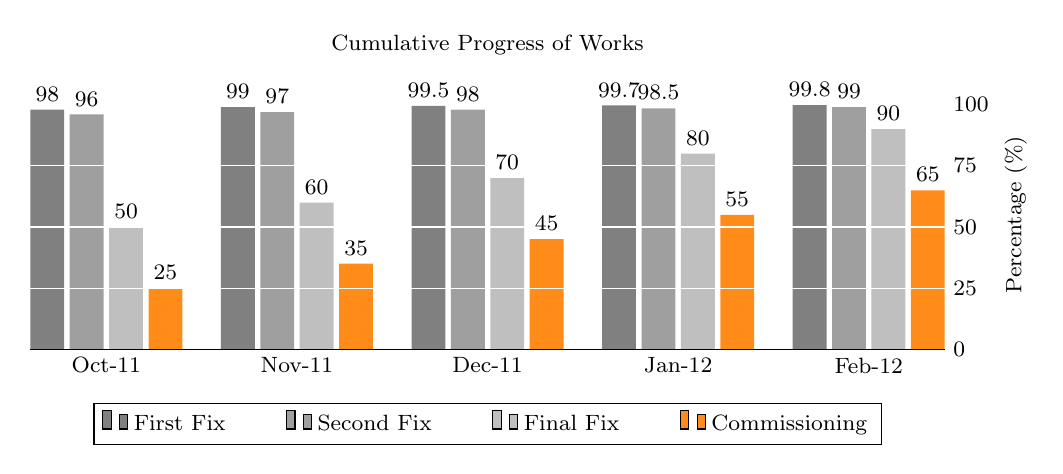
\begin{tikzpicture}
  \footnotesize
  \centering
  \begin{axis}[
        ybar, axis on top,
        title={Cumulative Progress of Works},
        height=5cm, width=13.2cm,
        bar width=0.43cm,
        ymajorgrids, tick align=inside,
        major grid style={draw=white},
        enlarge y limits={value=.1,upper},
        ymin=0, ymax=100,
        axis x line*=bottom,
        axis y line*=right,
        y axis line style={opacity=0},
        ytick={0,25,50,75,100},
        tickwidth=0pt,
        legend style={
            at={(0.5,-0.2)},
            anchor=north,
            legend columns=-1,
            % adds space between the legends
            /tikz/every even column/.append style={column sep=0.7cm}
        },
        ylabel={Percentage (\%)},
        symbolic x coords={
           Sep-11,Oct-11,Nov-11,Dec-11,
           Jan-12,Feb-12,
           Mar-12,
          Apr-12},
       xtick=data,
       nodes near coords={
        \pgfmathprintnumber[precision=2]{\pgfplotspointmeta}
       }
    ]
    \addplot [draw=none, fill=gray] coordinates {
      (Oct-11, 98)
      (Nov-11,99)
      (Dec-11,99.5)
      (Jan-12,99.7)
      (Feb-12,99.8)
       };
   \addplot [draw=none,fill=gray!75!white] coordinates {
      (Oct-11, 96)
      (Nov-11,97)
      (Dec-11,98)
      (Jan-12,98.5)
      (Feb-12,99)
        };
   \addplot [draw=none, fill=gray!50!white] coordinates {
      (Oct-11, 50)
      (Nov-11, 60)
      (Dec-11, 70)
      (Jan-12, 80)
      (Feb-12, 90)
            };
    \addplot [draw=none, fill=orange!90!white] coordinates {
      (Oct-11, 25)
      (Nov-11, 35)
      (Dec-11, 45)
      (Jan-12, 55)
      (Feb-12, 65)
          };
    \legend{First Fix,Second Fix,Final Fix,Commissioning}
  \end{axis}
  \end{tikzpicture}

\caption{\protect\raggedright Cumulative progress for all MEP works. Notice the slower rate of production during the last three months.}
\label{fig:tufte-overall}
\end{figure}


A good graph is uncluttered, clear and focused.

\subsection{Axis Lines}

Most problems with graphs arise from misuse of axes: too heavy, too long, wrong intersection,
ambiquous breaks or too confusing increments and incorrect proportions. An axis is a ruler that established
regular intervals for measuring the information provided. Axes may emphasize, diminish, distort, simplify
or clutter the information.

\clearpage
\begin{multicols}{2}
\subsection{Axis Length}

Graphs should utilize their space around them, as the graph itself is mostly white space. In publications the journal might want to minimize the cost of printing. An axis should not extend beyond the labeled unit od minor tick closest to the last data point.
\columnbreak
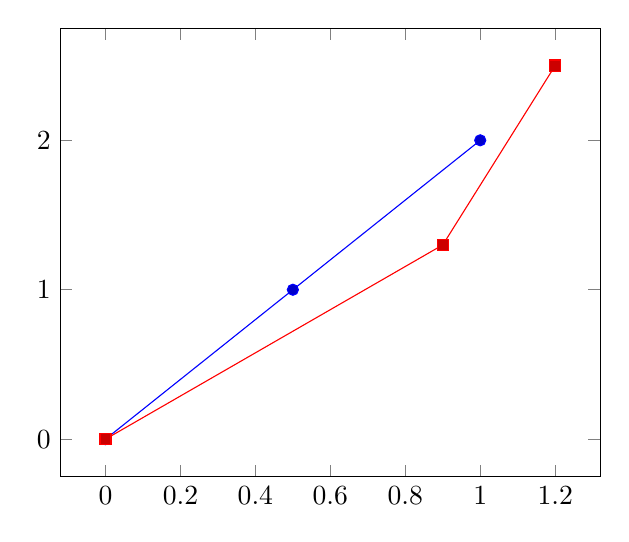
\begin{tikzpicture}
\begin{axis}
\addplot coordinates {
(0,0)
(0.5,1)
(1,2)
};
\addplot coordinates {
(0,0)
(0.9,1.3)
(1.2,2.5)
};
\end{axis}
\end{tikzpicture}
\end{multicols}


\section{The bullet graph}

The bullet graph is considered\footnote{\protect\url{http://www.perceptualedge.com/blog/?p=375}} to be a  better alternative to gauges in dashboards. A solution to a basic chart can be found at tx.se\footnote{\url{http://tex.stackexchange.com/questions/117314/is-there-any-package-to-create-bullet-gauge-graphs}}, by Jake, which sadly in a community of mathematicians, engineers and programmers was not popularized to the extend it deserved. 

Bullet gauges are commonly used to show the current state relative to a reference value with a background that divides the scale into regions.

\begin{figure}[htbp]
\centering

\includegraphics{./images/bullet-graph.png}
\caption{Bullet graph with annotations, indicating the various components of the graph.}
\end{figure}



current sales --
previous sales --
good -- 
great -- last shade box

Formatting: The color is preferable to be a range of distinct hues, which can also assist by those who are colorblind. It is also reproduced better when photocopies.  Intensities are preferred as follows:

three: 40\%, 25\% and 10\%

\makeatletter
\newenvironment {bulletgraph} {\luacode@begin\luacode@table@soft} {}
\makeatother

\pgfplotscreateplotcyclelist{bullet}{
{fill=color1, draw=none},
{fill=color2, draw=none},
{fill=color3, draw=none},
}

\pgfplotsset{mark options/.style={color=black!80}}
\pgfplotsset{barwidth/.style= {bar width=1.2ex} }
\pgfplotsset{chartheight/.style ={height=#1}}

\providecommand{\bulletgauge}[4][]{
    \begin{tikzpicture}[scale=0.8, font=\arial]
    \begin{axis}[
       width=8cm,
       chartheight = 60pt,
      % height=60pt,
       %y=2ex,
       xtick pos=left, 
       xtick = {0,50,...,400, 450},
       ytick=\empty,
       xmin=50, xmax=450,
        %enlarge y limits={abs=0ex},
        tick align=outside,
        axis on top,
        every axis title/.style={
            at={(rel axis cs:0,0.5)},
            anchor=east,
            align=right,
            xshift=-0.5em
        },
        #1
    ]
    \pgfplotsinvokeforeach{#4}{
        \pgfplotsset{cycle list name=bullet}
        \addplot +[xbar, bar width=7ex ] coordinates {(##1,0)};
    }
    \addplot [fill= barcolour, xbar, barwidth ] coordinates {(#2,0)};    
    \addplot [mark=|, mark options={very thick}, mark size=2ex, ] coordinates {(#3,0)}; 
    \end{axis}
    \end{tikzpicture}
}

\begin{scriptexample}{}{}
\begin{bulletgraph}
  m = require("i18n.bulletgraph")
 local data = {
     title = 'Valuation (Jan)',
     ranges = {230,300,500},
     bar = 200,
     marker = 220}
     local options = {
        barcolour = 'red!90'
   } 
m:render(data,options)        
\end{bulletgraph}
\medskip

\begin{bulletgraph}
   m = require("i18n.bulletgraph")
   local data = {
      title = 'Valuation (Apr)',
      ranges = {200,300,500},
      bar = 250,
      marker = 300}
   -- render the plot
   m:render(data,options)           
\end{bulletgraph}
\end{scriptexample}

Use an updated pgfplotsversion as we use |\pgfplotsset{compat=1.11}|, when we load the \pkgname{phd}. The environment |\begin{bulletgraph}|  is a |\luacode|  based environment and hence all the code has to be in lua syntax.

The code load the lua module |bulletgraph| and we the graph is rendered using the method \luacmd{render()}. The method, like most of the plotting routines provided by the package takes two arguments |data| and |options|.

\begin{texexample}{Bullet Plots}{ex:bulletplot}
\begin{bulletgraph}
local  bgraph = require("i18n.bulletgraph")
local data = {
     title = 'Valuation (Jan)',
     ranges = {230,300,500},
     bar = 200,
     marker = 220}
local options = {
        barcolour = 'red!90'
   } 
bgraph:render(data,options)        
\end{bulletgraph}
\end{texexample}

If you are familiar with Javascript you must have come across jQuery and its many plugins. The bulletgraph methods work in a similar fashion, where the options are a set of key values, that are used as a mixin with a set of default key values. If you only want to change the color of the bar, you only specify the color in the options the rest
are inherited from default values. All the \pkgname{phd} package routines, follow this design pattern to simplify the user interface and to enable typographical styles to be maintained throughout a publication. The best way to draw such charts is without the |options|. This separation of the interface, it also separates the data from the presentational aspects of drawing the plots.

\begin{texexample}{Bullet Plots (without options)}{ex:bulletplot1}
\begin{bulletgraph}
local  bgraph = require("i18n.bulletgraph")
local data = {
     title = 'Valuation (Jan)',
     ranges = {230,300,500},
     bar = 200,
     marker = 220}
bgraph:render(data,options)        
\end{bulletgraph}
\end{texexample}

\section{Using matplotlib}

Many researchers use Python to produce charts. A good guide can be found at \href{https://github.com/jbmouret/matplotlib_for_papers}{jbmournet} at github. There was also a good discussion at HN\footnote{\protect\url{https://news.ycombinator.com/item?id=9043571}}.












%  ^^A \chapter{WRAPPED ILLUSTRATIONS}
\parindent2em
\let\onepar\lorem

If you are planning to have a more traditional book design wrapped figures are essential. Traditional typographers used
all sorts of styles to achieve this is to use
The best way to achieve it is to use Donald Arseneau's wrafig package.

\begin{wrapfigure}{l}{3.2cm}
    \includegraphics[width=3cm]{amato}
    \caption{\footnotesize Wrapped figures}
\end{wrapfigure}

Get prepared to do a lot of manual adjustments, see your figures disappear on page refreshes and reruns. After a while though you get the hang of it and by minor adjustments you can really achieve great results. The manual uses \verb+everypar+ to insert commands for the shaping of the paragraphs that \emph{follow} the wrapped figure.

Wrapfig.sty provides the environments \pkg{wrapfigure} and \pkg{wraptable} for typesetting a
narrow float at the edge of the text, and making the text wrap around it. The wrapfigure
and wraptable environments interact properly with the \verb+\caption+ command to produce
proper numbering, but they are not regular floats like figure and table, so (beware!)
they may be printed out of sequence with the regular floats. The environment  provides one of those monster commands that stresses one's memory as itprovides for four parameters. 
The four param
for \verb+\begin{wrapfigure}+, two optional and two required, plus the text of the figure, with a caption perhaps.

\begin{macro}{wrapfigure}
\end{macro}

|\begin{wrapfigure}[12]{r}[34pt]{5cm}\meta{figure}\end{wrapfigure}|

  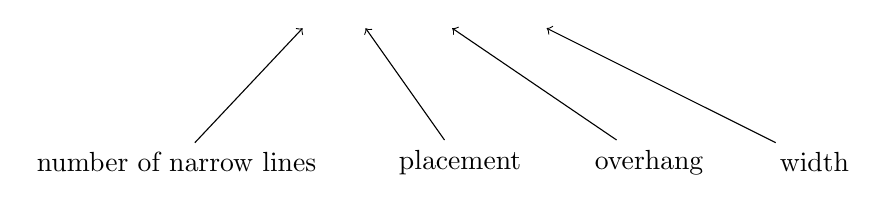
\begin{tikzpicture}[xshift=-15pt]
    \node (number) at (0mm, 0mm) {\oarg{number of narrow lines}};
    \node (placement) at (36mm, 0mm) {\marg{placement}};
    \node (overhang) at (60mm, 0mm) {\oarg{overhang}};
    \node (width) at (81mm, 0mm) {\marg{width}};
    \begin{scope}[->]
    \draw (number) -- (16mm, 17mm);
    \draw (placement) -- (24mm, 17mm);
    \draw (overhang) -- (35mm, 17mm);
    \draw (width) -- (47mm, 17mm);
    \end{scope}
  \end{tikzpicture}


First we will look at placing the figure without the use of optional commands.


\begin{verbatim}
\begin{wrapfigure}{r}{.4\textwidth}
    \includegraphics[width=.4\textwidth]{./path/file}
    \caption{\footnotesize Wrapped figures}
\end{wrapfigure}
\end{verbatim}

From the four parameters the first one indicates if the figure is to be typeset left or right.

\begin{verbatim}
\begin{wrapfigure}{l}{\imagewidth}
    \includegraphics[width=\imagewidth



]{./graphics/parasol-01}
    \caption{\footnotesize Wrapped figures}
\end{wrapfigure}
\end{verbatim}


\begin{wrapfigure}[16]{I}[0.1pt]{85pt}
    \vskip-10.5pt plus 2pt minus 2pt\relax
    \includegraphics[width=83pt]{parasol-01}
    \caption{\scriptsize Wrapped figures, parameters set at \texttt\{l\}\{90pt\}.}
\end{wrapfigure}

Changing the parameters to suit we now have the illustration floating to the left. Allowing for the figure to be approximately two point  wider than the actual graphic, will leave a bit more margin. If the figure is end low in the page you need to be careful, that it does not disappear, as you will not get any warning.

The first parameter we are going to use an optional parameter is the one that determines the number of narrow lines. The format is \verb+[narrowlines]{l}{90pt}+. Think of this parameter as a fine tuning parameter and do not touch it until after your final draft is ready. If you see indented lines at the beginning of the page that follows the wrapped figure, reduce the number of lines, until you get satisfactory results.

The second optional parameter, comes after the \texttt{\{r\}[overhang]} parameter.

The second optional parameter (\#3) tells how much the figure should hang out into
the margin. The default overhang is given by the length \verb+\wrapoverhang+, which is 0pt
normally but can be changed using |\setlength|. For example, to have all wrapfigures
use the space reserved for marginal notes,

\begin{verbatim}
\setlength{\wrapoverhang}{\marginparwidth}
\addtolength{\wrapoverhang}{\marginparsep}
\end{verbatim}

Again not recommended. The best approach is to specify the figures with O or I, let them float and if the results are
not very good then make manual adjustments. Get prepared to spend at least 5-10 minutes fiddling with the final result.

When you do specify the overhang explicitly for a particular figure, you can use a
special unit called \string\width meaning the width of the figure. For example, [0.5\string\width]
makes the center of the figure sit on the edge of the text, and [\string\width] puts the figure
entirely in the margin (and the adjacent text is indented by just \string\columnsep). This
\texttt{\string\width} is the actual width of the wrapfigure, which may be greater than the declared
width.

\begin{figure}[tb]
\includegraphics[width=\textwidth]{chiefs}
\caption{Chiefs of Kelau or Kelaou.}
\label{fig:chiefs}
\end{figure}

\begin{figure}[p]
\centering

\includegraphics[width=0.8\textwidth,height=0.9\textheight, keepaspectratio]{parasol-01}
\caption{Chiefs of Kelau or Kelaou.}
\label{fig:parasol-01}
\end{figure}

\section{Balancing the illustrations}

Illustrations come in various sizes, but in general they need to flow with the text. Place figures on top of the page and figures that would dominate the text on their own page. For example Figure~\ref{fig:chiefs} was allowed to float to the top of a page whereas Figure~\ref{fig:parasol-01} was placed on its own page, as I thought it will overwhelm the text if shown in a large size. However the same figure seems perfectly alright as a wrapped figure.

\begin{texexample}{}{}
\begin{wrapfigure}{I}{0pt}
    \includegraphics[width=75pt]{parasol-01}
 \end{wrapfigure}
\lipsum[1-2]
\begin{wrapfigure}{l}{0pt}
    \includegraphics[width=75pt]{parasol-01}
 \end{wrapfigure}
\lipsum[1-2]
\end{texexample}



\begin{texexample}{}{}
\begin{wrapfigure}{l}{0pt}
    \includegraphics[width=70pt]{parasol-01}
    \includegraphics[width=70pt]{parasol-01}
 \end{wrapfigure}

\lipsum[1-3]\lorem
\end{texexample}




\begin{texexample}{}{}
\begin{wrapfigure}[13]{L}{0pt}
    \includegraphics[width=100pt]{conicalbasket}
\end{wrapfigure}

\onepar\onepar\onepar

\end{texexample}




%  ^^A \chapter{Colors}
\section{Introduction}

One area where \latex shows its age is the manipulation and use of colors. When \tex was developed color printing was not possible and the introduction of colors is now only predominantly via the use of the |xcolor| package. Despite such limitations colors can be used fairly easily.

\newthought{The figure below, shows the wavelengths} in nm of the visible light. It has been drawn using the \docpkg{xcolor} package and the native \latex environment \cs{picture}. The colors can be typest using the wavelength of light.

\smallskip

\begin{texexample}{}{}
  \hbox{\color{thered} A TesT}
\end{texexample}




\newcount\WL \unitlength.75pt

\begin{figure}
\hskip-3pt\scalebox{0.9}{
\noindent

\begin{picture}(460,60)(355,-10)
\sffamily \tiny \linethickness{1.25\unitlength} \WL=360
\multiput(360,0)(1,0){456}%
{{\color[wave]{\the\WL}\line(0,1){50}}\global\advance\WL1}
\linethickness{0.25\unitlength}\WL=360
\multiput(360,0)(20,0){23}%
{\picture(0,0)
\line(0,-1){5} \multiput(5,0)(5,0){3}{\line(0,-1){2.5}}
\put(0,-10){\makebox(0,0){\the\WL}}\global\advance\WL20
\endpicture}
\end{picture}}
\caption{The visible spectrum nm}
\end{figure}

The |xcolor| package provides numerous macros for typesetting colors, using a variety of methods and color schemes. For example we can use the command \cs{color} to print a text sample in color.
\newlength\pull

\def\colorSample#1{%
\leavevmode
\parindent0pt
   \def\colorRule{\color[wave]{#1}\rule{\textwidth}{0.4pt}} 
   \colorRule
%% set to the width of the box
   \settowidth\pull{\framebox{\Large #1 nm}}
%% pull by one em
   \addtolength\pull{1em}
   \hskip -\pull{\color[wave]{#1}{{\framebox{\Large #1 nm}}}}%
%% add story
   \hskip1em\noindent\onepar\par
   \colorRule
}
\bgroup
\colorSample{385}
\colorSample{809}
\egroup


\section{Specifying colors by name}

The easier way to specify colors is to use the pre-build names available
with the package drivers.


\section{Color boxes}

Now and then users want to place text in colorboxes. The macro \cs{colorbox} can be used to provide background text to a box.

\begin{macro}{\colorbox}
The colorbox macro takes one command. As it is modelled on the same concept as an
\cs{fbox} it will add a bit of space around the containing text. If you want
to remove it you will have to set the \cs{fboxsep=0pt}.
\end{macro}


\begin{texexample}{Color boxes}{}
\fboxsep0pt
\colorbox{green}{\begin{minipage}{3cm}
  Some text
\end{minipage}}

\fboxrule.2pt\fboxsep-.2pt
\fbox{\begin{minipage}{3cm}
  Some text
\end{minipage}}
\end{texexample}

\begin{macro}{\textcolor}
The \cs{textcolor} takes two arguments and typesets the contents of the second argument, using the color specified in the first argument.
\end{macro}

\begin{texexample}{Color text}{}
\textcolor{blue}{This is typeset in blue color.}

\end{texexample}

\section{Mixing colors}

Colors can be mixed by using a convention using (!).

\begin{texexample}{Mixing colors}{}
\color{blue!40!yellow}
\lorem
\end{texexample}

One can also mix colors from different color schemes and |xcolor| will take care of the calculations.

\section{Defining colors}

There are two commands that one can use to define colors.

\begin{macro}{\definecolor}\oarg{type}\marg{name}\marg{model-list}\marg{spec-list} 
The |\definecolor| command is one of the commands that may be used to assign a \textit{name} to a specific color. Afterwards, this color is known to the system (in the current group) and may be used in color expressions. Note that an existing color name will be overwritten.
\end{macro} 

\begin{texexample}{Defining colors}{}
\definecolor{red}{rgb}{1,0,0}
\definecolor{mygray}{named}{black}
\colorlet{myblack}{black}

\color{myblack}\lorem
\end{texexample}

\section{Palettes}

The \pkgname{phd} offers the concept of a palette. A palette is a set of colours that can be used to colour sectioning and other document elements in a consistent and easy way.

It also offers the misnamed command \cmd{\inherit} that allows the inheritance of a color from a higher level section to a lower level.

If you study the styling commands each and every sectioning command has a colour attribute. This colour attribute if not set it defaults to the standard color used for sectioning in palettes.

\cxset{palette/.store in=\palette}

document text color
document headings color
document 












%  \makeatletter
%  ^^A \chapter{The \texttt{picture} Environment}
\label{pictureenvironment}
\index{environments!picture}

The |picture| environment comes straight out of the box and can be used to draw simple figures. For more sophisticated graphics |TikZ| is a better choice. It can be used in package documentation and simple tasks. The learning curve for using it is minimal.

\section{The Basic Commands}

\begin{macro}{picture}
The |picture| environment is created using one of two commands.
\end{macro}

\emphasis{picture}
\begin{teXXX}
 \begin{picture}(x, y). . . \end{picture}
\end{teXXX}

\noindent or

\begin{teXX}
  \begin{picture}(x, y)(x0,y0). . . \end{picture}
\end{teXX}

\begin{macro}{\unitlength}
Most people prefer the first type which they combine, with a |setlength| command that sets the \cs{unitlength}.
\end{macro}

The optional argument gives the coordinates of the point at the lower-left corner of the picture (thereby determining the origin). For example, if \cs{unitlength} has been set to 1mm, the command

\begin{texexample}{}{}
  \setlength\unitlength{1mm}
  \begin{picture}(40,40)(0,0)
    \put(10,30){\vector(0,-1){30}}
    \put(10,30){\vector(1,0){30}}
    \put(25,30.5){$a$} 
  \end{picture}
\end{texexample}

produces a picture of width 100 millimeters and height 200 millimeters, whose lower-left corner is the point (10,20) and whose upper-right corner is therefore the point (110,220). When you first draw a picture, you will omit the optional argument, leaving the origin at the lower-left corner. If you then want to modify your picture by shifting everything, you just add the appropriate optional argument.

\section{Text and Formulae}

\begin{macro}{\linethickness}
\begin{macro}{\thicklines}
\begin{macro}{\thinlines}
Text and formulas can be written into a picture
environment with the \cs{put} command in the usual way. The line thickness can be
set by using \cs{linethickness}\marg{dim}. The command \cs{thinlines} is half the thickness of the \cs{linethickness} dimension and \cs{thicklines} is the current line width. The \cs{linethickness} does not change width of slanted lines
or circles as it is drawn using a font and would render badly.
\end{macro}
\end{macro}
\end{macro}

\emphasis{thicklines}
\begin{texexample}{Text and Formulae}{}
\setlength{\unitlength}{0.8cm}
\begin{picture}(6,5)
 \thicklines
 \put(1,0.5){\line(2,1){3}}
 \put(4,2){\line(-2,1){2}}
 \put(2,3){\line(-2,-5){1}}
 \put(0.7,0.3){$A$}
 \put(4.05,1.9){$B$}
 \put(1.7,2.95){$C$}
 \put(3.1,2.5){$a$}
 \put(1.3,1.7){$b$}
 \put(2.5,1.05){$c$}
 \put(0.3,4){$F=
 \sqrt{s(s-a)(s-b)(s-c)}$}
 \put(3.5,0.4){$\displaystyle
 s:=\frac{a+b+c}{2}$}
\end{picture}
\end{texexample}



\setlength{\unitlength}{5cm}
\begin{picture}(1,1)
\put(0,0){\line(0,1){1}}
\put(0,0){\line(1,0){1}}
\put(0,0){\color{blue}\line(1,1){1}}
\put(0,0){\color{orange}\line(1,2){0.5}}
\end{picture}


\section{multiput and linethickness}
The \cmd{multiput} is used to place multiple objects onto the picture. It has the general format shown below:

\setlength{\unitlength}{2mm}
\begin{picture}(30,20)
  \color{green}
   \linethickness{0.075mm}
   \multiput(0,0)(1,0){25}%
   {\line(0,1){20}}
   \multiput(0,0)(0,1){21}%
   {\line(1,0){25}}
   \linethickness{0.15mm}
   \multiput(0,0)(5,0){6}%
   {\line(0,1){20}}
   \multiput(0,0)(0,5){5}%
   {\line(1,0){25}}
   \linethickness{0.3mm}
   \multiput(5,0)(10,0){2}%
    {\line(0,1){20}}
   \multiput(0,5)(0,10){2}%
   {\line(1,0){25}}
\end{picture}

The multiput command has the general format shown below.

|\multiput(x, y)(Dx,Dy){n}{object}|

\begin{figure}
\setlength{\unitlength}{0.8cm}
\begin{picture}(6,5)
 \thicklines
 \put(1,0.5){\line(2,1){3}}
 \put(4,2){\line(-2,1){2}}
 \put(2,3){\line(-2,-5){1}}
 \put(0.7,0.3){$A$}
 \put(4.05,1.9){$B$}
 \put(1.7,2.95){$C$}
 \put(3.1,2.5){$a$}
 \put(1.3,1.7){$b$}
 \put(2.5,1.05){$c$}
 \put(0.3,4){$F=
 \sqrt{s(s-a)(s-b)(s-c)}$}
 \put(3.5,0.4){$\displaystyle
 s:=\frac{a+b+c}{2}$}
\end{picture}
\caption{Figures can have captions, if you enclose in a figure environment}
\end{figure}

\begin{figure}
\scalebox{0.7}{
\setlength{\unitlength}{0.5mm}
\begin{picture}(120,168)
\newsavebox{\foldera}
\savebox{\foldera}
(40,32)[bl]{% definition
\multiput(0,0)(0,28){2}
{\line(1,0){40}}
\multiput(0,0)(40,0){2}
{\line(0,1){28}}
\put(1,28){\oval(2,2)[tl]}
\put(1,29){\line(1,0){5}}
\put(9,29){\oval(6,6)[tl]}
\put(9,32){\line(1,0){8}}
\put(17,29){\oval(6,6)[tr]}
\put(20,29){\line(1,0){19}}
\put(39,28){\oval(2,2)[tr]}
}
\newsavebox{\folderb}
\savebox{\folderb}
(40,32)[l]{% definition
\put(0,14){\line(1,0){8}}
\put(8,0){\usebox{\foldera}}
\put(0.2,1.4)
{$\beta=v/c=\tanh\chi$}
}
\put(34,26){\line(0,1){102}}
\put(14,128){\usebox{\foldera}}
\multiput(34,86)(0,-37){3}
{\usebox{\folderb}}
\end{picture}}
\caption{Pictures can be scaled using \protect\textbackslash scalebox.}
\end{figure}

\section{Some examples}
Any vertex-symmetric graph is regular, but edge-symmetric graphs
need not be regular. For example,
\begin{verbatim}
$$\unitlength=10pt
\def\putdisk(#1,#2){\put(#1,#2){\disk{.4}}}
$\vcenter{
\hbox{\beginpicture(2,1.5)(0,0)
\putdisk(0,0)
\putdisk(2,0)
\putdisk(1,.5)
\putdisk(1,1.5)
\put(0,0){\line(2,1){1}}
\put(2,0){\line(-2,1){1}}
\put(1,.5){\line(0,1){1}}
\endpicture}}
\quad&\hbox{is edge-symmetric, not vertex-symmetric;}\cr
\noalign{\smallskip}
\vcenter{
\hbox{\beginpicture(2,2)(0,0)
\putdisk(1,0)
\putdisk(1,2)
\putdisk(0,.5)
\putdisk(0,1.5)
\putdisk(2,.5)
\putdisk(2,1.5)
\put(0,.5){\line(2,1){2}}
\put(2,.5){\line(-2,1){2}}
\put(0,.5){\line(2,3){1}}
\put(2,.5){\line(-2,3){1}}
\put(0,.5){\line(1,0){2}}
\put(0,1.5){\line(1,0){2}}
\put(1,0){\line(-2,3){1}}
\put(1,0){\line(2,3){1}}
\put(1,0){\line(0,1){2}}
\endpicture}}
\quad&\hbox{is vertex-symmetric, not edge-symmetric.}\qquad
 (\vcenter{\hbox{\beginpicture(1,2)(0,0)
\putdisk(.5,0)\putdisk(.5,2)\put(.5,0){\line(0,1){2}}\endpicture}}
\hbox{ is a maximal clique})\cr}$$
\end{verbatim}



\section{picture package}

The \pkg{picture} package by Heiko Oberdiek redefines the default \pkg{picture} macros and adds code that detects
whether such an argument is given as number or as length. In the latter case, the
length is used directly without multiplying with \cs{unitlength}. Th following
example i from the documentation of the package.

 \setlength{\unitlength}{1pt}
 \begin{picture}(\widthof{Hello World}, 10mm)
   \put(0, 0){\makebox(0,0)[lb]{Hello World}}%
   \put(0, \heightof{Hello World} + \fboxsep){%
   \line(1, 0){\widthof{Hello World}}%
 }%
 \put(\widthof{Hello World}, 10mm){%
   \line(0, -1){10mm}%
 }%
 \put(0,0){\line(966,259){8}}
 \end{picture}

The package |calc| is used for calculations or etex. The picture package requires that the package |calc| is loaded before
the |picture| package and is loaded correctly by |phd|.

The package also supports the packages \pkg{pspicture} and \pkg{pict2e}, but they must be loaded before package picture.

\section{pict2e}

The package pict2e by Hubert G\"a\ss lein, Rolf Niepraschk and Joseph Tkadlec extends the existing LATEX picture environment, using the familiar
technique (cf. the graphics and color packages) of driver files. In the user-level part of
this documentation there is a fair number of examples of use, showing where things are
improved by comparison with the Standard LaTeX picture environment.

The package is loaded automatically by |phd|.







% 
% ^^A 
LATEST
%  

\makeatletter
\cxset{toc image=\@empty}

\@specialtrue
\setdefaults 
\renewcommand\stewart[2][]{%
\fancypagestyle{fancy}{%
\lhead{}\rhead{}
\chead{}
\cfoot{}
\lfoot{}
\rfoot{\thepage}
\def\footrule#1{{\color{blue}%
  \hrule width\paperwidth}\vskip3pt
}

\renewcommand{\headrulewidth}{0pt}
\renewcommand{\footrulewidth}{0.4pt}}

\clearpage

\begin{tikzpicture}[remember picture,overlay]
% Main shading block
\node [xshift=5cm,yshift=-\paperheight] at (current page.north west)
[text width=0.98\textwidth,text height=\paperheight, fill=thecream!30,rounded corners,above right]
{};
\node [xshift=6.5cm,yshift=-1.5cm-\soffsety] at (current page.north west)
[text width=0.9\textwidth,below right]{\sffamily \bfseries \huge #2};

\node [xshift=3cm,yshift=-1.5cm] at (current page.north west)
[text width=3cm,align=center,minimum height=2.5cm, fill=blue,below right]
{\[\text{\HHUGE\bfseries\sffamily\color{white}\thechapter}\]
\par\vspace*{3pt}
};

\node [xshift=-0.2cm,yshift=-21.5cm] at (current page.north west)
[text width=3cm,above right]%
{\includegraphics[width=1.0\paperwidth]{./chapters/\image@cx}};
% second box left
\node [xshift=3cm,yshift=-19.5cm] at (current page.north west)
[text width=9cm,minimum height=2.5cm,inner sep=0.5em, fill=blue,below right]
{\color{white}
  \bfseries\sffamily \texti@cx
};
% Last block
\node [xshift=6.5cm,yshift=-26cm] at (current page.north west)
[text width=12cm,above right]
{\textii@cx
};
\end{tikzpicture}
\par
\clearpage
}





\cxset{steward,
  numbering=arabic,
  custom=stewart,
  offsety=0cm,
  image=hine03,
  texti={When Lamport designed the original \LaTeX\ sectioning commands he did not provide a fully comprehensive interface for modifying their design. With current tools available improvements are much easier to program and this chapter provides the details.},
  textii={\precis{In this chapter we discuss a method that allows the production of fancy chapter headings and formatting, based on a set of key values. Central  to this process is the separation of content from presentation.
We also discuss the basic formatting tools that are available and how one can modify them to mould new book designs.}
 }
}


\chapter{Designing Chapters}

\section{Introduction}

For too long, the act of printing something in and of itself has been placed on too high a pedestal. The true value of an object lies in what it says, not its mere existence. And in the case of a book, that value is intrinsically connected to content. The aim of this package is to try and provide a bridge between separating content from presentation.

A new chapter must make a good impression and must give an immediate signal that something different is going to be written. Traditionally chapter openings in LaTeX are an unimpressive and dry event. Our aim is to brighten it up a bit, while keeping true separation of content from presentation.



\section{Package Usage}

To use the package include it just like any other package:

\begin{tcolorbox}
\begin{lstlisting}
\documentclass{book}
\usepackage{chaptersx}
\cxset{style13}
\begin{document}
\chapter{Introduction}
\end{document}
\end{lstlisting}
\end{tcolorbox}

The command \cs{cxset} sets the default style for the example to the style defined as \marg{style13}. The package currently offers over 50 styles and numerous keys to manipulate them further.



\section{Chapter opening page}

The standard LaTeX classes offer only two options to either open a chapter on an odd page or at any page. This package offers five alternatives:

\keyval{chapter opening}{\marg{any, left, right, anywhere, ifafter}}{The various keys enable any combination to be used.}

\begin{marglist}
\item [any] Opens a chapter at any page, either verso or recto.
\item [left] Opens a chapter on an even page
\item [right] Opens a chapter on a right page.
\item [anywhere] Opens a chapter at the point where the \cs{chapter} is typed.
\item [none] Alias for \marg{anywhere}.
\item [ifafter] Opens a chapter at the next page if the page has material that does not exceed a certain portion of \cs{textheight}.
\end{marglist}

To change a setting you just modify the value of the key \option{chapter opening} to one of the values described earlier.

\begin{tcolorbox}
\begin{lstlisting}
\cxset{chapter opening=anywhere}
\end{lstlisting}
\end{tcolorbox}

\@specialfalse
\cxset{chapter toc=false}
\begin{texexample}{title=Inline Chapter Example}{ex:anywhere}
\cxset{chapter opening=anywhere, chapter before=\bigskip, chapter font-family=\sffamily,title font-family=\sffamily}

\lipsum[2]
\chapter{Chapter Example}
\lipsum[3]
\chapter{Another Chapter Example}
\lipsum[4]
\end{texexample}



\addtocounter{chapter}{-1}

Examples for other types of chapter openings follow in the rest of the documentation.

\subsection{Blank pages before chapters}
In the standard LaTeX book class when the openany option is not given or in the report class when the openright is given, chapters start at odd-numbered pages. This can cause a blank page to be printed. Some book designers prefer this page to be completely empty, without any headers or footers. This cannot be done with \lstinline{\thispagestyle} as this command will have to be issued on the \textit{previous} page. However by a suitable redefinition of the
\lstinline{\clearpage} this can be done automatically.
\medskip

\begin{tcolorbox}
\begin{lstlisting}
\makeatletter
\def\cleardoublepage{\clearpage\if@twoside\ifodd\c@page\else
  \hbox{}
  \vspace*{\fill}
  \begin{center}
    This page left intentionally blank.
  \end{center}
  \vspace{\fill}
  \thispagestyle{empty}
  \newpage
  \if@twocolumn\hbox{}\newpage\fi\fi\fi}
\makeatother
\end{lstlisting}
\end{tcolorbox}
\medskip

This is achieved easily by setting the following options:
\bigskip

\begin{tcolorbox}
\lstinline{chapter blank page=empty}\par
\lstinline{chapter blank page text=Some text.}\par
\lstinline{chapter blank page=plain}\par
\end{tcolorbox}
\medskip



The last one refers to a \lstinline!\thispagestyle{plain}!.

\section{Keys for chapter head formatting}

A chapter heading can be considered of being constructed of several parts, the \textit{chapter number}, the chapter name typically \textit{chapter} and the \textit{title}. Predefined keys handle all the elements of formatting. Additional keys are defined to handle other elements such as inclusion of images or producing complicated examples with graphics constructed with TikZ or other similar packages.

\medskip

\keyval{chapter numbering font-size}{\oarg{sizing commands}}{}.
\keyval{chapter numbering font-family}{\oarg{sizing commands}}{}.

\subsection{Keys for numbering}
Chapter numbering follows that of the standard \LaTeX\ classes and is extended to cover some additional cases such as fully spelled out numbers.

\keyval{number numbering}{\oarg{alph,Alph,roman,Roman,none,WORDS,words}}{Style of numbering.}
\medskip

\parindent1.5em

Note that the package uses Heiko Oberdiek's package alphalph to allow for alphabetic numbering that extends beyond the normal 26 letters of the alphabet. Examples for numbering can be seen in \ref{ex:romannumbering}

\medskip




\begin{marglist}
\item [arabic] Despite that the Arabs call what the West calls Arabic numbers Indian numbers, we provide the value arabic to have normal numbers printed.
\item [alph] Lowercase alphabetic numbering.
\item [Alph] Uppercase alphabetic numbering.
\item [roman] Lowercase roman numbering.
\item [Roman] Uppercase roman numbering.
\item [words]
\item [WORDS]
\item [Words] Prints the number in words and capitalizes the first letter, for example the number 21 will be printed as `Twenty One'\footnote{Currently limited to the first hundred numbers}.
\item [none] This is equivalent to using the star version of the command. It does not print any number and does not increment the chapter counter.\footnote{I am ambivalent about this, perhaps it will be better to increment it, as it can give a more general approach.}
\end{marglist}

\cxset{chapter opening=anywhere, numbering=Roman}
\index{chapter design!numbering!roman}
\begin{texexample}{Setting up keys for numbering}{ex:romannumbering}
\cxset{numbering=Roman}
\chapter{Roman numbering}
\end{texexample}



\clearpage

\index{chapter design!numbering!words}
\begin{texexample}{title=Chapter number in words}{}
\cxset{numbering=WORDS}
\chapter{Literal numbering}
\end{texexample}



\cxset{numbering=arabic}
\subsection{Setting font information}
\subsection{Letter spacing}

Chapter letter spacing can be achieved using the soul package in a combination with the key spaceout.
\medskip



\keyval{chapter spaceout}{\marg{soul}}{Uses the soul package to space out the lettering of chapter, number or the chapter name.}\par\medskip



The following examples illustrate the usage.

\begin{texexample}{}{}
\cxset{numbering=Roman,
         chapter spaceout=none,
         title spaceout=soul,
         title font-size=\Large,
         title font-family=\rmfamily,
         title font-shape=\scshape}
\chapter{Letter Spacing}
\end{texexample}



\index{chapter design!labels!letter spacing}
\begin{texexample}{}{} 
\cxset{chapter spaceout=soul,numbering=arabic, title spaceout=soul}
\chapter{Chapter title}
\end{texexample}



\subsection{Styling the title}

Similarly to the number and chapter styling keys exist for styling the title. We summarize the available standard keys below:
\medskip

  \keyval{chapter title font-family}{\marg{family}}{Selects a predefined font family}
  \keyval{chapter title font-weight}{\marg{\cs{bfseries},\cs{normalseries}}}{Font weight.}
  \keyval{chapter title font-size}{\marg{\cs{large},\cs{Large},\cs{huge},\cs{Huge},\cs{HUGE},\cs{HHuge}}}{Font sizing command.}
  \keyval{chapter title font-color}{}{}
  \keyval{chapter title spaceout}{\marg{soul,none}}{}
  \keyval{title before}{}{}
 \keyval{title after}{}{}
  \keyval{title beforeskip}{}{}
  \keyval{title afterskip}{}{}


\begin{texexample}{letter spacing the chapter title block}{}
\cxset{style13, chapter spaceout=none,
       numbering=arabic}
\chapter{Chapter Title Styling}
\end{texexample}



The last example illustrated the use of a predefined style \oarg{style13} and overriding some of the parameters.


\cxset{chapter opening=right}
\section{Table of Contents}\index{table of contents!key settings}

Traditionally a chapter will be added to the Table of Contents if the \cs{chapter} command is issued. The starred version will not produce a number and will not add a contents line. Since we have adopted an approach where we use a key value interface we can dispense with the starred version of the command, by setting the \option{chapter toc} option to false. For example if we want to define a command for a ``Foreward'' or ``Epiloque'' without wishing them to be added to the table of contents we can use the following setting.\index{Foreward!definitions}\index{Epilogue!definitions}



\begin{texexample}{changing the chapter label name}{}
\cxset{chapter toc=false, name=, numbering=none,}
\chapter{Foreward}
\lorem
\end{texexample}

Note that the key \option{numbering=none} still has to be set.


Please note that when \textbf{numbering=none} the chapter number is not available anymore and yo may have to reset it if required again. Although this might be seen as rather cumbersome than simply using \cs{chapter*} the advantage is consistency in the user interface and the use of appropriate semantic definitions for all sectioning commands thus achieving a bit more separation of context from style.


\cxset{chapter toc=true}

\section{Defining styles}

Named styles can be defined using the standard \textsc{PGF} conventions. To define a style for the forward above we can use:

\begin{texexample}{}{}
\cxset{foreward/.style={chapter toc=false,numbering=none,
          name=,
          title font-size= Large,
          title font-family= sffamily,
          numbering=none}}
\cxset{foreward}
\chapter{Foreward.}
\lorem
\end{texexample}



\cxset{numbering=arabic}
\section{Creating semantic names for commands and environments}

To keep our search for semantic commands and true separation of contents it is prudent to define some macros for typesetting the  `foreward' section.

\begin{texexample}{defining a \textit{Foreward} macro.}{}
\begin{lstlisting}
\cxset{foreward/.style={chapter toc=false,
          name=,
          title font-size = Large,
          title font-family = sffamily,
          numbering=none}}
\newcommand\forewardname{foreward}
\expandafter\newenvironment\expandafter{\forewardname}{%
\cxset{foreward}\chapter{Foreward}}%
{}
\begin{foreward}
\lorem
\end{foreward}
\end{lstlisting}
\end{texexample}



Notice the use of a new command \cs{forewardname} to allow for internationlization using Babel or other methods. One is tempted to let the English name, but a better approach perhaps is to define both.



%  \makeatletter\@specialfalse
\cxset{custom = stewart}
\cxset{steward,
  numbering=arabic,
  custom=stewart,
  offsety=0cm,
  image={./images/hine03.jpg},
  texti={When Lamport designed the original \LaTeX\ sectioning commands he did not provide a fully comprehensive interface for modifying their design. With current tools available improvements are much easier to program and this chapter provides the details.},
  textii={\precis{In this chapter we discuss a method that allows the production of fancy chapter headings and formatting, based on a set of key values. Central  to this process is the separation of content from presentation.
We also discuss the basic formatting tools that are available and how one can modify them to mould new book designs.}
 }
}


\cxset{epigraph rule color=teal,epigraph width=0.37\textwidth\relax}

\chapter{Epigraphs}\index{epigraphs}
\label{c:epigraphs}

\epigraph{Please give examples of good use of epigraphs in fiction.

I mean them quoted dealies they sometimes put at the start of chapters.

What counts as ``good use" is whatever you think counts. Part of my goal is to understand what people like about these things.
.}{\href{http://ask.metafilter.com/207423/Good-use-of-epigraphs-in-fiction}{Stebulus}}



\section{Introduction}

Epigraphs or quotations before or after chapters are quite common in books. Peter Wilson's epigraph package \citep{epigraph}, 
does a good job and we have adapted it where necessary to allow for a key value interface. The command:

\cs{epigraph}\marg{text}\marg{source}. By default the epigraph is placed at the right
hand side of the textblock, and the \marg{source} is typeset at the bottom right of the \marg{text}. 
Numerous settings allow for manipulating the width of the epigraph, the location and other 
variables. If the package is available we use it otherwise we use other internal commands.

All key values for epigraphs, start with the keyword \emph{epigraph}. You can think of the epigraph of a block of text that can go anywhere on a page and has some formatting rules that are set 

\section{Key-value interface}
The key value interface provided by the package is shown below. It mostly follows the 
naming conventions of the epigraph package to make the transition easier for experienced users. Use any dimension or a dimension expression.
\medskip

\begin{key}{/phd/ epigraph width = \marg{dim}}
  Sets the width of the epigraph block. 
\end{key}


\begin{key}{/phd/ epigraph align = \marg{left\textbar center\textbar right}}
 A font-size command such as \cs{footnotesize}, 
\cs{small} and other similar commands. This will align the full block containing the epigraph, left right or center according to the setting of the key. Most epigraphs are aligned right.
\end{key}

\cxset{epigraph align=left, epigraph width=300pt}
\epigraph{Example is the school of mankind, and they
will learn at no other.}{\texttt{epigraph align=left, epigraph width = 300pt}}


\begin{key}{/phd/ epigraph rule width = \marg{dim}}
 The width of the rule separating the epigraph from the source. Set to 0pt,if you do not want a rule.
\end{key}

\begin{key}{/phd/ epigraph font-size = \marg{font sizing cmd}}  Use a font sizing command such as \cmd{\footnotesize}
\end{key}

\begin{key}{/phd/ epigraph beforeskip = \marg{dim}}
Space before the epigraph.
\end{key}

\begin{key}{/phd/ epigraph afterskip = \marg{dim}}
Space after the epigraph.
\end{key}

\subsection{Styling the source part}

\begin{key}{/phd/ epigraph source align = \marg{left\textbar center\textbar right}}
Align the source text to the right, left or center.
\end{key}

\begin{key}{/phd/ epigraph source font-size=\marg{dim}}Align the source text to the right, left or center.
\end{key}

\begin{key}{/phd/ epigraph source font-shape = \marg{dim}}
Align the source text to the right, left or center.
\end{key}

\begin{key}{/phd/ epigraph source font-family = \marg{dim}}Align the source text to the right, left or center.
\end{key}


\begin{key}{/phd/epigraph source font-weight = \marg{bold,normal}}
Align the source text to the right, left or center.
\end{key}


Usage examples can be found in relevant style examples (See Chapter~\ref{ch:41}) for a rather 
nice example with non-traditional alignment.

\section{Epigraphs on empty pages}

When a chapter open on an odd page sometimes the  previous page is left empty. Some book designers 
add the words ``this page left intentionally blank'' and other might add a quote. To add such a quote use:

\begin{tcolorbox}
\begin{lstlisting}
\cxset{blank page text=\epigraph{The great tragedy of science is the slaying of a beautiful theory
by an ugly fact.}{Thomas Huxley}}
\end{lstlisting}
\end{tcolorbox}

%  \makeatletter\@specialtrue\makeatother
\cxset{custom = stewart}
\cxset{steward,
  numbering=arabic,
  custom=stewart,
  offsety=0cm,
  image={./images/hine03.jpg},
  texti={When Lamport designed the original \LaTeX\ sectioning commands, limitations of computer power forced him to restrict the abstraction of complicated chapter layouts. With current tools available improvements are much easier to program.},
  textii={In this chapter we discuss a method that allows the production of fancy section headings and formatting, based on a set of key values. Central  to this process is the separation of content from presentation.
We also discuss the basic formatting tools that are available and how one can modify them to mould new book designs.
 }
 }



\chapter{Lower Level Headings}


\section{Introduction}

Good book design dictates that sectioning styles follow that the general book design and theme. An academic publication for example might have chapters and section numbered in arabic numerals, whereas a high school textbook might have sections marked in colored boxes.

Similarly to the chapter key value interface, the package offers a key value interface to adjust sectioning command parameters.



\cxset{section afterskip={10pt}}
\renewsection

\section{Section styling}

In a similar fashion to the chapter commands the following keys are provided.

\subsection{Fonts and numerals}

Font and numeral keys are shown below.
\medskip
\begin{key}{/phd/section font-size= \marg{sizing commands}} The font-size command takes arguments
of the  type |Large|, |large| both as commands or without the backslash, which is the recommended way
of setting styles with the |phd| package. 
\end{key}

\begin{docKey}[phd] {section font size} {= \marg{sizing commands}} {normal size} 
All the font commands, come in two flavours,
with a hyphen or without, in order to present a user interface that is similar to |pgf/TikZ| conventions for that
are familiar with \latex and another for those used to |CSS| conventions.
\end{docKey}

\begin{key}{/phd/section font-family}{= \marg{sizing commands}}{no default, initial value normal} The font-family key, accepts normal LateX values
related to families, but if LuaTeX or XeLaTeX are present it can also accept commands created with |\newfontfamily| 
command of the |fontspec| package, which is loaded automatically by the |phd| package. The package has a database of a number of human friendly names for fonts and commands. If one of these are detected the
family is created at run-time to avoid overloading too many fonts at start-up. 
\begin{verbatim}
\cxset{section font-family = Arial}
\cxset{section font-family = sffamily}
\cxset{section font-family = ttfamily}
\end{verbatim}
The family command family name (if undeined by the user), defaults to the human friendly version name but without the spaces. 
\end{key}

%
%  \keyval{section font-weight}{\marg{cmd}}{Font weight command such as \cs{bfseries.}}
%  \keyval{section font-family}{\marg{cmd}}{Font family command such as \cs{sffamily.}}
%  \keyval{section font-shape}{\marg{cmd}}{Font shape command such as \cs{itshape}}
%  \keyval{section color}{\marg{color}}{Color of section.}
%  \keyval{section numbering}{\marg{arabic|roman|Roman|alph|Alph|words|WORDS}}{Section number style.}
  \begin{marglist}
  \item [arabic] Typesers the section number in arabic numerals.
  \item [roman] Typesets the section number in lowercase roman numerals.
  \item [Roman] Typesets the section number in uppercase roman numerals.
  \item [alph] Typesets the section number in lowercase alphabetic numbering.
  \item [Alph] Typesets the section number in uppercase alphabetic numerals.
  \item [words] Typesets the numbers in words (lowercase).
  \item [WORDS] Typesets the number in words (uppercase).
  \end{marglist}

\subsection{Skip and indentation commands}

The keys for indentation and above and below skips are shown below.
\medskip

\keyval{section beforeskip}{}{}
\keyval{section afterskip}{}{}
\keyval{section indent}{\marg{dim}}{Indentation from margin as per standard LaTeX class definitions.}
\keyval{section spaceout}{}{}
\begin{marglist}
 \item[soul]
 \item[none]
\end{marglist}



\subsection{align}

\keyval{section align}{\marg{cmd}}{One of the alignment commands centering, ragged right, raggedleft}

\subsection{Hooks}

Hooks for adding material are shown in the following sketch.
\medskip

\fbox{aboveskip}

\fbox{indent} \fbox{number}\fbox{hook}\fbox{title}

\fbox{belowskip}


\section{Example usage}

In our first example we will use a predefined style for the chapter headings, so we do not need to clutter the example with the chapter commands that we have previously discussed. Our first example will number the section in lower roman, enclosed in brackets and center it.


\makeatletter\@specialfalse
\cxset{
 chapter toc=false,
 chapter  name=CHAPTER,
 numbering=arabic,
 number font-size=huge,
 number font-family=sffamily,
 number font-weight=bfseries,
 number before=,
 number dot=,
 number after=\hspace{1em},
 number position=rightname,
 chapter opening=anywhere,
 chapter font-family=sffamily,
 chapter font-weight=bfseries,
 chapter font-size=huge,
 chapter before={\vspace*{0.1\textheight}\hfill},
 chapter after={\hfill\hfill\vskip0pt\thinrule\par},
 chapter color=black!90,
 number color= black!90,
 title beforeskip={\vspace*{30pt}},
 title afterskip={\vspace*{30pt}\par},
 title before={\hfill},
 title after={\hfill\hfill},
 title font-family=\sffamily,
 title font-color= black!90,
 title font-weight=bfseries,
 title font-size=huge,
 section font-size= LARGE,
 section font-weight= bold,
 section font-family= sffamily,
 section align= centering,
 section numbering=arabic,
 section indent=0em,
 section align= centering,
 section beforeskip=20pt,
 section afterskip=10pt,
 section font-shape= itshape,
}

\cxset{book/.style={
 section numbering=arabic,
 section font-size=Large,
 section font-weight=bfseries,
 section font-family=rmfamily,
 section font-shape=normalfont,
 section align=\raggedright,
 subsection font-size=\large
 section indent=0em,
 section beforeskip=-3.5ex \@plus -1ex\@minus -0.2ex,
 section afterskip=2.3ex\@plus.2ex,
 subsection beforeskip=-3.5ex \@plus -1ex\@minus -0.2ex,
 subsection afterskip= 1.5ex \@plus .2ex,
}}
\makeatother


\begin{texexample}{Adjusting section parameters}{ex:sec}
\cxset{ section font-size= LARGE,
 section font-weight= bold,
 section font-family= sffamily,
 section font-shape=upshape,
 section numbering=(roman), 
 section indent=0em,
 section align= centering,
 section beforeskip=20pt,
 section afterskip=10pt,}
\chapter{A First Look at the Sectioning Keys}
\section{First section}
\lorem
  % adjust counter number so it does not affect the
  % rest of the document
\addtocounter{section}{-1}
\end{texexample}


The keys are mostly self-explanatory. We have used a |beforeskip| and |afterskip| without any glue. The numbering is just a continuation of the document sections. 

One notable thing to keep in mind is that the numbering of the chapter is independent of that for the section, so if you need to have strange combinations rather define a section numbering custom.\index{section formatting!vertical space}

\cxset{section numbering=arabic}
\subsection{Adjusting vertical spaces}

Perhaps the most important issues we need to consider is the adjusting of vertical spaces; example~\ref{ex:latex}, that follows illustrates settings from the Octavo class and compare them with those of standard the \LaTeXe\ book class. The Octavo class through settings that are based on baselineskip fractions and multiples endeavours to achieve a grid layout. The class also tones down the `loudness' of some of the headings compared to those of the book class.

\makeatletter
\cxset{octavo/.style={
 section font-size=large,
 section font-weight=,
 section font-family=rmfamily,
 section font-shape=scshape,
 section indent=0em,
 section align=\centering,
 section beforeskip=-1.666\baselineskip\@minus -2\p@,
 section afterskip=0.835\baselineskip \@minus 2\p@,
 section after indent = false,
 subsection numbering=none,
 subsection font-family= rmfamily,
 subsection font-size=,
 subsection font-shape=scshape,
 subsection font-weight=,
 subsection indent=1em,
 subsection align=RaggedRight,
 subsection beforeskip=-0.666\baselineskip\@minus -2\p@,
 subsection afterskip=0.333\baselineskip \@minus 2\p@,
 subsection color=spot!50,
 subsubsection color=spot!50,
 }}

\renewsection
\renewsubsection
\renewsubsubsection


\cxset{book/.style={
 section numbering=arabic,
 section font-size= Large,
 section font-weight= bfseries,
 section font-family= rmfamily,
 section font-shape= upshape,
 section align= RaggedRight,
 subsection font-size= large,
 section indent=0em,
 section beforeskip=-3.5ex plus -1ex minus -0.2ex,
 section afterskip=2.3ex plus 0.2ex,
 subsection font-size= large,
 subsection font-weight= bfseries,
 subsection numbering=arabic,
 subsection indent=0pt,
 subsection beforeskip=-3.5ex \@plus -1ex\@minus -0.2ex,
 subsection afterskip= 1.5ex \@plus .2ex,
}}

\cxset{octavo headings/.style={
 section numbering=none,
 section font-size=Large,
 section font-weight=,
 section font-family=rmfamily, section font-shape= scshape,
 section indent=0em, 
 section align=centering, 
 section afterindent=off,
 section beforeskip=-1.666\baselineskip\@minus -2\p@,
 section afterskip=0.835\baselineskip \@minus 2\p@, 
 %
 subsection numbering=none,
 subsection font-family=\rmfamily, 
 subsection font-size=, subsection font-shape=scshape,
 subsection font-weight=, subsection indent=1em, 
 subsection align= RaggedRight,
 subsection beforeskip=-0.666\baselineskip\@minus -2\p@,
 subsection afterskip=0.333\baselineskip \@minus 2\p@,
 subsubsection numbering=none,
 subsubsection font-family= rmfamily,
 subsubsection font-size=,
 subsubsection font-shape= itshape,
 subsubsection font-weight=,
 subsubsection indent = 0em,
 subsubsection align= raggedright,
 subsubsection beforeskip=-0.666\baselineskip\@minus -2\p@,
 subsubsection afterskip=0.333\baselineskip \@minus 2\p@,
 subsubsection color=spot!50,
 paragraph numbering=none,
 paragraph font-family= rmfamily,
 paragraph font-size=,
 paragraph font-shape=itfamily,
 paragraph font-weight=,
 paragraph color = spot!50,
 paragraph indent=0em,
 paragraph align= RaggedRight,
 paragraph beforeskip=10pt,
 paragraph afterskip=1em,
}}
\makeatother
\renewsection \renewsubsection \renewsubsubsection \renewparagraph

\cxset{octavo headings}


%\begin{texexample}{Octavo class headings, settings}{}
%\cxset{octavo headings/.style={
% section numbering=none,section font-size=large,
%section font-weight=,
% section font-family=rmfamily, section font-shape=scshape,
% section indent=0em, 
% paragraph numbering=none,
% paragraph font-family=rmfamily,
% paragraph font-size=,
% paragraph font-shape=,
% paragraph font-weight=,
% paragraph indent=-1em,
% paragraph align=raggedright,
% paragraph beforeskip= 0pt,
% paragraph afterskip=0pt,
%}}
%
%\cxset{octavo headings}
%\renewsection\renewsubsection\renewsubsubsection
%\section{Octavo Class Heading}
%\lorem
%\subsection{Octavo subsection}
%This is some text short text\par
%\subsubsection{Octavo sub-subsection}
%\lorem
%\paragraph{paragraph heading} This is some short text.
%\makeatother
%\end{texexample}


The following example was set using the |style| |\cxset{Octavo headings}| with some minor adaptations to enable us to show it inline with the rest of the material on this page\footnote{We set it using \cs{cxset}\marg{chapter opening = anywhere}}. We kept the use of a typical colour throughout the text, whereas the Octavo class, does not allow the use of color.

\cxset{chapter opening = anywhere,
          chapter color = spot!50,
          title font-color = spot!50,
          chapter name={},
          chapter numbering = none,
          chapter before = \addvspace{\baselineskip},
          chapter after = ,
          title spaceout=soul,
          title before =,
          title afterskip=\bigskip\bigskip,
          number before=,
          number after=,
          }
          
\bgroup
\parindent=0pt
\par

\chapter{Octavo Chapter Heading}
\lorem

\section{Octavo Class Heading (Section) }
\lorem

\subsection{Octavo subsection}
\lorem

\subsubsection{Octavo sub-subsection}
\lorem

\paragraph{Paragraph heading} This is some short text.
\lorem

\paragraph{paragraph heading} This is some short text.
\lorem

\egroup


\begin{texexample}{\LaTeXe\ book class headings settings}{ex:latex}
\makeatletter
\cxset{book/.style={
 section numbering prefix = \thechapter.,
 section numbering=arabic,
 section number after=,
 section font-size= Large,
 section font-weight=bfseries,
 section font-family=rmfamily,
 section font-shape=upshape,
 section align=RaggedRight,
 section beforeskip=10pt,
 section spaceout = none,
 section color  = red,
 subsection font-size=large,
 section indent=0em,
 section beforeskip=-3.5ex \@plus -1ex\@minus -0.2ex,
 section afterskip=2.3ex\@plus.2ex,
 subsection color = blue,
 subsection font-size=large,
 subsection font-shape=upshape,
 subsection font-weight=bfseries,
 subsection numbering prefix=\thesection.,
 subsection numbering = arabic,
 subsection beforeskip=-3.5ex \@plus -1ex\@minus -0.2ex,
 subsection indent= 0pt,
 subsection afterskip= 1.5ex \@plus .2ex,
}}

\cxset{book}

\renewsubsection

\section{LaTeX Book  Class Heading}
\lorem
\subsection{A subsection}
\lorem
\makeatother
\end{texexample}



\section{Grid example}

One problem sometimes is that the sectioning commands create problems with grid layouts. Example~\ref{ex:grid} shows example settings.

\begin{texexample}{Section styles from the grid package}{ex:grid}
\makeatletter
\cxset{grid/.style={
 section numbering=arabic,
 section font-size=,
 section font-weight=bfseries,
 section font-family=rmfamily,
 section font-shape=upshape,
 section beforeskip=-.999\baselineskip,
 section afterskip=0.001\baselineskip,
 section align= RaggedRight,
 subsection font-size=,
 section indent=0em,
 subsection font-shape=,
 subsection font-weight=bfseries,
 subsection numbering=arabic,
 subsection indent=0pt,
 subsection beforeskip=1\baselineskip,
 subsection afterskip= -.35\baselineskip,
 subsubsection font-shape=itshape,
 subsubsection font-weight=bfseries,
 subsubsection numbering= none,
 subsubsection indent=0pt,
 subsubsection beforeskip=1\baselineskip,
 subsubsection afterskip= -.35\baselineskip,
}}
\cxset{grid}



\renewsubsection
\begin{multicols}{2}
\section{Grid  Class Heading}
\lorem
\subsection{Grid  subsection.}
\lorem
\subsubsection{A subsection grid.}
\lorem
\subsubsection{Another subsection grid.}
\lorem
\end{multicols}
\makeatother
\end{texexample}



The key \option{\bfseries section numbering custom}=\marg{code} is quite powerfull and can be used to define any type of section number style. Just remember that the numbering so far depends on two counters, the c@chapter and c@section. What the section numbering does, it redefines the macro \cs{thesection} to the new definition provided as argument for the key.

Although the temptation to define a lot of key combinations one would rather define new styles as a more user friendly approach.

\cxset{section numbering=arabic, section align= RaggedRight, section font-shape=upshape, section font-family=rmfamily}
\section{Handling Other Section Levels}

Other sectioning commands such as \cs{subsubsection}, \cs{paragraph} and \cs{subparagraph} have equivalent keys. Examples can be found in the chapters that follow for specific styles.

\section{Technical discussion}

The standard LaTeX classes, book report and article have sections showing dot leaders, whereas in the article class the sections are shown without the dotted lines, as the |\l@section| macro is redefined for articles. With the \pkgname{phd} the distinction is unecessary and style files can do the trick that is, either load style article or book or for that matter any other style that has the relevant settings.

\index{macros!\textbackslash @seccntformat}

\subsection{Lower Section Headings}

\LaTeXe\ offers two pathways in redefining section commands, the first one is \refCom{@startsection} and the second is \refCom{@seccntformat} \index{sectioning macros}. It also uses the macro \cs{secdef} to create the starred and unstarred versions of the sectioning commands.

\begin{tcolorbox}{}
\begin{lstlisting}
% \begin{macro}{\l@section}
%    In the article document class the entry in the table of contents
%    for sections looks much like the chapter entries for the report
%    and book document classes.
%
%    First we make sure that if a pagebreak should occur, it occurs
%    \emph{before} this entry. Also a little whitespace is added and a
%    group begun to keep changes local.
% \changes{v1.0h}{1993/12/18}{Replaced -\cs{@secpenalty} by
%    \cs{@secpenalty}.  ASAJ.}
% \changes{v1.2i}{1994/04/28}{Don't print a toc line when the tocdepth
%    counter is less than 1.}
% \changes{v1.4a}{1998/10/12}{we should use \cs{@tocrmarg}; see PR/2881.}
%    \begin{macrocode}
%<*article>
\newcommand*\l@section[2]{%
  \ifnum \c@tocdepth >\z@
    \addpenalty\@secpenalty
    \addvspace{1.0em \@plus\p@}%
%    \end{macrocode}
%
%    The macro |\numberline| requires that the width of the box that
%    holds the part number is stored in \LaTeX's scratch register
%    |\@tempdima|. Therefore we put it there. We begin a group, and
%    change some of the paragraph parameters (see also the remark at
%    \cs{l@part} regarding \cs{rightskip}).
%    \begin{macrocode}
    \setlength\@tempdima{1.5em}%
    \begingroup
      \parindent \z@ \rightskip \@pnumwidth
      \parfillskip -\@pnumwidth
%    \end{macrocode}
%    Then we leave vertical mode and switch to a bold font.
%    \begin{macrocode}
      \leavevmode \bfseries
%    \end{macrocode}
%    Because we do not use |\numberline| here, we have do some fine
%    tuning `by hand', before we can set the entry. We discourage but
%    not disallow a pagebreak immediately after a section entry.
%    \begin{macrocode}
      \advance\leftskip\@tempdima
      \hskip -\leftskip
      #1\nobreak\hfil \nobreak\hb@xt@\@pnumwidth{\hss #2}\par
    \endgroup
  \fi}
%</article>
\end{lstlisting}
\end{tcolorbox}



As you can see the dot leaders are not present in the above definition. Although we can get rid of dot leaders in other section by redefining them, it is not as easy to add them back.

As our aim is to be able to have all the classes used a common denominator we can define a command as follows (using book as a base)

\begin{tcolorbox}{}
\begin{lstlisting}
\def\articlesection{
\newcommand*\l@section[2]{%
  \ifnum \c@tocdepth >\z@
    \addpenalty\@secpenalty
    \addvspace{1.0em \@plus\p@}%
    \setlength\@tempdima{1.5em}%
    \begingroup
      \parindent \z@ \rightskip \@pnumwidth
      \parfillskip -\@pnumwidth
      \leavevmode \bfseries
      \advance\leftskip\@tempdima
      \hskip -\leftskip
      #1\nobreak\hfil \nobreak\hb@xt@\@pnumwidth{\hss #2}\par
    \endgroup
  \fi}
}
\end{lstlisting}
\end{tcolorbox}


\begin{docCommand}{@startsection}{}
The \cs{@startdsection} macro is one of those locomotive type of commands. It takes 7 required arguments and 2 optional ones and hidden within it are two booleans. The full set looks like this:

\cs{@startsection} \marg{name} \marg{level} \marg{indent} \marg{beforeskip} \marg{afterskip} \marg{style}[*]
  [\marg{altheading}]\marg{heading}.
\end{docCommand}

\begin{marglist}
\item[name] The name of the level command.
\item [level] A number denoting the depth of the section, chapter=1, section=2, etc. A section number will be printed only if \marg{level} is equal or smaller than the value of \textit{secnumdepth}
\item[indent] The indentation of the heading from the left margin.
\item[beforeskip]  The absolute value of this argument is the skip to leave above the heading. If it is negative, then the paragraph indent of the text following the heading is suppressed.
\item [afterskip] If positive, it is the skip to leave below the heading, else it is the skip to the right of a run-in heading.
\item [style] Sets the style of the heading.
\item[\textup{[*]}] When this is missing the heading is numbered and the corresponding counter is incremented.
\item[\textup{[\textit{altheading}]}] Gives an alternative heading to use in the table of contents and in the running heads. This should be present when the * form is used.
\item[heading] The heading of the new section.
\end{marglist}

\begin{texexample}{Example formatting run-in section}{}
\makeatletter
\bgroup
\renewcommand\section{
    \@startsection{section}
    {1}
    {0em}
    {-0.8em}
    {-0.5em}
    {\large\normalfont\scshape}}
\makeatother
\section[]{test}
\lorem
\egroup
\end{texexample}



Note we run the example in a group so that we will not influence the formatting of this document.

As mentioned earlier there is an additional way to introduce formatting for sections and this is using the command \cs{@seccntformat}, which is responsible for typesetting the counter part of a section title. The default definition of the command typesets the \cs{the} representation of the section counter.

\begin{texexample}{}{}
\bgroup
\renewcommand\section{%
    \@startsection{section}%
    {1}%
    {0em}%
    {-0.8em}%
    {-0.5em}%
    {\large\normalfont\scshape}}
\renewcommand\@seccntformat[1]{\fbox
{\csname the#1\endcsname}\hspace{0.5em}}
\makeatother
\section[]{test}\label{sec:ok}
\lorem

See section \ref{sec:ok}.
\egroup
\end{texexample}



\cxset{section color=spot!50,
          subsection color = spot!50 }
          
\section{Custom headings}

\begin{docCommand*}{@secdef}{}
So far we have used the |phd|’s keys to set keys that are affecting the standard commands used by
\latexe to set headings. Another way to achieve this,  is to use the macro
 \cs{@secdef}. Therefore, if you wish to use different definitions of \cs{@seccntformat}
for different headings, you must put the appropriate code into every heading
definition.
\end{docCommand*}



\begin{phdverbatim}
\newcommand\part{\secdef\starcmd\unstarcmd}
\end{phdverbatim}

The |part| and |chapter| and sometimes |appendix| are defined this way, but nothing stops us from doing the same for other sectioning commands. What the \cs{secdef} command does it will produce the definitions required for a star or unstarred version of the sectioning command, such as |\section|.\footnote{See \ttfamily File F: ltsect.dtx Date: 2014/09/29 Version v1.0z 360} 

\begin{texexample}{}{}
\bgroup
\makeatletter
\renewcommand\section[2] [?]{%
    \refstepcounter{section}
    \addcontentsline{toc}{section}
    {\protect\numberline{section-\thesection}#1}
    {\raggedright\large\bfseries SECTION-\thesection\par \centering#2\par}
    \sectionmark{#1}
    \@afterheading 
   \addvspace{\baselineskip}
 }%
\section[test]{Section Heading}
\lorem
\makeatother
\egroup
\end{texexample}

Many other strategies can also be implemented that are perhaps easier to grasp.

\begin{teX}
\def\@seccntformat##1{\csname the##1\endcsname{}}
\end{teX}


\begin{texexample}{}{}
\makeatletter
\bgroup
\def\strut{\vrule height12pt depth1pt width0pt}
  \renewcommand\section[2] []{% % Complex form:
  \refstepcounter{section}% % step counter/ set label
  \addcontentsline{toc}{section}% % generate toc entry
  {\protect\numberline{\thesection} }%
  {\raggedright\large\bfseries\scshape %
  \parbox[b]{\dimexpr(\linewidth-0.5\columnsep)}{\colorbox{brown!80}%
  {{\vbox{\strut\raise2pt\hbox{#2}}}}}}\vskip0pt% % and number
  \sectionmark{#1}% % add to running header
  \@afterheading % prepare indentation handling
  \vspace{\dimexpr\baselineskip+6pt}%must have a parameter
}
\chapter{Fossil Insects}
\begin{multicols*}{2}\raggedcolumns
\section[Insect Fossilization]{\raggedright \thinspace Insect Fossilization}
\lipsum[1]
\end{multicols*}
\egroup
\makeatother
\end{texexample}


Of course some work is needed to center the text properly in the middle of the colour box. For all practical purposes it is lining up as per the sample.

In Chapter we discussed a forward, but this may not apply if there are no chapters or we need to treat these as sections, the example \ref{ex:forwardsection} shows such a method.


\begin{texexample}{Defining a Foreward Section}{ex:forwardsection}
\makeatletter
\newcommand\prematter@sp[1]{
\addcontentsline{toc}{section}
{\protect\numberline{}#1}
\sectionmark{#1}
{\LARGE\centering\normalfont\sffamily\colorbox{brown!80}{ \textsc{#1}}\par}%
\@afterheading
\addvspace{\baselineskip}
\@afterindentfalse
}

\newenvironment{prematter}[1]{%
   \prematter@sp{#1}}
{}
\begin{multicols}{2}
\label{theok}
\begin{prematter}{Foreward}
\lipsum[1]
\end{prematter}\ref{theok}
\end{multicols}
\makeatother
\end{texexample}


\section{underlining}

I am aware that some people have no choice but have some sections underlined as dictated by archaic regulations in some establishments for thesis submission. If nobody is forcing you to underline it is best to avoid it. We use Donald Arsenau's ulem package to achieve underlining. \footnote{\protect\url{http://tex.stackexchange.com/questions/52998/change-title-to-small-caps-but-not-in-toc}}


\makeatletter
\gdef\sectionopen{}
\def\@sectionsuffix{}
\def\@sectionprefix{\sectionname\space}
\newif\if@sectioncase \@sectioncasefalse

\cxset{
  section special/.code =\def\specialsection@cx{#1},
  section xcolor/.store in = \sectionxcolor@cx,
  section opening/.is choice,
  section opening/openany/.code=\gdef\sectionopen{\clearpage},
  section opening/right/.code = \gdef\sectionopen{\cleardoublepage},
  section opening/none/.code = \gdef\sectionopen{},
  section top rule/.is choice, 
  section top rule/true/.code =\DeclareRobustCommand\sectiontoprule{%
        \leavevmode\par\noindent\rule{\textwidth}{1pt}\vskip3.5pt},
  section top rule/true/.code=\def\sectiontoprule{\leavevmode\par\noindent\tikzrule},      
  section top rule/false/.code=\gdef\sectiontoprule{},
  % bottom rule
  section bottom rule/.is choice, 
  section bottom rule/true/.code =\DeclareRobustCommand\sectionbottomrule{%
        \leavevmode\par\noindent\rule{\textwidth}{1pt}\vskip.5pt},
  section bottom rule/true/.code=\def\sectionbottomrule{\vskip-0.5\baselineskip\rlap{\tikzrule}},      
  section bottom rule/false/.code=\gdef\sectionbottomrule{},
  % upper and lower case - TODO in lua
  section case/.is choice,
  section case/lower/.code=\def\sectioncase@cx{\@sectioncasetrue
                             \if@sectioncase\expandafter\MakeTextLowercase\fi},
  section  case/upper/.code=\def\sectioncase@cx{\@sectioncasefalse
                    \if@sectioncase\else\expandafter\MakeTextUppercase \fi},
  section  case/none/.code=\def\sectioncase@cx{\@empty},
}
\cxset{
          section special = sectionspecialruled@cx,
          section xcolor=spot!50,
          section afterindent=false,
          section opening=right,
          section top rule=true,
          section bottom rule=true,
          section afterskip=20pt,
          section case=lower,
          section font-family=aegean
          }


%\def\specialsection@cx{sectionspecialruled@cx}
\def\secdef#1#2{\@ifstar{\@dblarg{#2}}{\@dblarg{#1}}}
%
\newcommand\sectionx{%
  \par  
  \sectionopen   %determines if it is to be treated like a chapter
  \addpenalty\@secpenalty\nobreak
  \secdef\sectionspecialruled@cx\@ssection
   } 
  

% The macro sectionspecial@cx is a more generic macro that typesets the block of tex
% for the section heading.
% 
\def\sectionspecialruled@cx[#1]#2{%
   \sectiontoprule
  \ifnum\c@secnumdepth>0\relax
     \refstepcounter{section}%
     \addcontentsline{toc}{section}{%
      \@sectionprefix\thesection\@sectionsuffix
       \texorpdfstring{\quad}{ }#1}%
  \else
     \addcontentsline{toc}{section}{#1}%
  \fi
  {% start the title
    \color{\sectionxcolor@cx}%
    \noindent\centering\interlinepenalty\@M
   \setfont@cx{\sectionfontweight@cx}%
       {\sectionfontfamily@cx}{\sectionfontsize@cx}{\sectionfontshape@cx}%
     \ifnum\c@secnumdepth>0\relax
        \@sectionprefix\thesection\@sectionsuffix
        \quad\sectioncase@cx{#2}%
    \else %
       \sectioncase@cx{#2}
      % \luadirect{tex.print(string.upper(#2))}%
   \fi%
   \sectionbottomrule
   %\expandafter\addvspace\sectionafterskip@cx\relax%
%   \tikzrule 
   %\rule{\textwidth}{3pt}%
   \afterindent@cx
   \nobreak\par}}


\def\@ssection[#1]#2{%
  \phantomsection
  \addcontentsline{toc}{section}{#1}%
  {\noindent\centering\interlinepenalty\@M
   \color{\sectioncolor@cx}
     \setfont@cx{\sectionfontweight@cx}%
       {\sectionfontfamily@cx}{\sectionfontsize@cx}{\sectionfontshape@cx}%
       \sectiontoprule
       
        \sectioncase@cx{#2}%
        \sectionbottomrule
       %\expandafter \addvspace\sectionafterskip@cx \relax
      \afterindent@cx
   \nobreak\par}}
\makeatother

\let\section\sectionx

\section{Special Sections}

When we described the usage of the chapter setting keys, we extended the system to describe commands
for specially constructed chapter heads that do not follow the normal style of \latexe.

This section describes how to design and program, sectioning styles that go a little bit more than those that
can be defined so far and that they will require you to have a bit more knowledge of \tex and \latexe programming skills.

For example, the heading of this section started on a new page and has rules above and below the title and section number. In addition the title was capitalized automatically, despite having been typed as:

\begin{verbatim}
\section{Special Sections}
\end{verbatim}

By setting the key and calling the section again, we can typeset it on the same page

\begin{verbatim}
   \cxset{section opening=none}
   \section{Another example}
\end{verbatim}

\cxset{section opening=none,
          section case=upper,
          section top rule=false,
          section bottom rule=true,
          section afterindent=false}
          
\section{Another example}

Special sections have their own user provided macros, that have been pre-defined by the user and are invoked using the key |section special|. In the example below we have predefined a macro |\sectionsspecialruled@cx|.
Do not use a command in the value just the literal name of the command as shown below,

\begin{verbatim}
\cxset{section special = ruled,}
\end{verbatim}

\cxset{section opening=none,
          section case=none,
          section top rule=true,
          section bottom rule=false}
          
The star section of the command omits the section number from the heading. It will still insert an entry into the toc. If it is provided with an optional argument it will insert the optional text into the toc.

Check the Table of Contents to see the rendering.

\begin{verbatim}
\section*{No number test}
\section*[Short Title]{No number test}
\end{verbatim}

\section*{No number test}
\lorem

\cxset{section bottom rule=true,
         section afterindent=false,
         section font-family=agean}

\section*[Short Title]{No number test}

\lorem

\cxset{chapter opening=any,
          chapter toc=true,
          chapter numbering=arabic}

One can extend these \emph{specials} to much more complicated sections (which can resemble) chapter openings.
\makeatletter 
\newif\if@debug \@debugtrue
\bgroup
\leftskip-3cm \rightskip2cm
\def\hook{\node[right=5pt, yshift=-12pt] at (0,-3) {\HUGE\color{purple} This is the  Title}; }
\def\hook{}

\cxset{chapter name = CHAPTER}
%\expandafter\ifnum\thechapter=0\stepcounter{chapter}\else\fi

\hspace*{-2cm}\begin{tikzpicture}
\if@debug\draw [help lines] (0,0) grid (18,-13);\else\fi
\draw[fill=red]  (0,0) circle (1.5pt) ;
\node[rectangle,draw, right, baseline] (x) at (0,1) {\LARGE\color{black!30}{before}\relax};
\draw[fill=red]  (0,1) circle (1.5pt) ;
\node[rectangle,draw, right=1sp] at (0,0) {\LARGE\color{black!20} \so\chaptername\relax};

\node[rectangle,draw, color=white, below right, fill=blue!50, text=white] at +(\textwidth,0) {\scalebox{2}{\HUGE \thechapter}};
\draw[fill=red]  (0,-3) circle (1.5pt) ;
% The title of the block
\node[rectangle, draw, text width=9cm,below right, yshift=-1pt] at (0,-3) {%
         \sffamily
         \HUGE Title Format\vskip1sp \medskip\Large Blue colors in jeans, dresses skirts\\ and hats.\\
         How to dress in stylish blues. \\Getting your partner to get\\ into LaTeX. }; 
\node at (12.5,-9) {\includegraphics[width=7cm]{./images/fashion.jpg}};
\hook
\end{tikzpicture}
\makeatother
\tikzrule 
\egroup 

For such complex layouts, it is always best to start from a piece of paper where you roughly outline
the design of the template. I call such layouts templates, because we will insert a number of variables
to parameterize them. All the typesetting commands will need to be inserted in a macro, which you
should give it a unique name. We will name the above template \emph{fashion} and we will later on define
a macro \cmd{\fashion}. The sectioning mechanism provided by the \pkgname{phd} will enable the
setting of such layouts to be carried out as:

\begin{verbatim}
\cxset{section custom = fashion}
\end{verbatim}

Everytime we call the above in our document settings, in the preamble or elswehere or subsequent sections will
be typeset using this format. 

Also before you get into too much detail in programming you should define the \emph{new} parameters
that may have to be introduced. In the example above most of the fields are already defined either
using the |phd|  key value interface or by LaTeX itself. What is new here is only the introduction of an image
and perhaps some rules as to its exact location. For example you can establish a rule that if half the width of
the image is less than the right margin then it should be centered at the right side of the textblock, alternatively it should be lined at the end of the page. We will see how to achieve this a bit later on.

It is also best to start with a MWE and to first achieve the layout you want without any parameters being introduced. We assume that we will be using TikZ to position the text and the image exactly where we 
want them, although nothing stops us from using either plain TeX boxes or the picture environment.
Since we are loading the TikZ package it is best though to use it for the graphical layout.

Introduce a |debug| boolean to help you with switching grid lines on and off. Depending on what you are trying to accomplish you may want to also add some hooks into the definitions. Start from the layout first.

\begin{verbatim}
\begin{tikzpicture}
\if@debug
   \draw [help lines] (0,0) grid (18,-13);
\else
\fi
...
\fashionposthook
\end{tikzpicture}
\end{verbatim}

We draw a grid of $18\times13$ cells which just happens to suit this particular layout well; The command 
\cmd{\fashionposthook} was just added to provide any further tikz instructions at runtime.

We then draw the layout first as best as we can and without too much consideration for parameterizing the layout at this stage.

\emphasis{if@debug,else,fi}
\begin{scriptexample}{}{}
\begin{teX}
\begin{tikzpicture}
\if@debug
  \draw [help lines] (0,0) grid (18,-13);
  \draw[fill=red]  (0,0) circle (1.5pt) ;
  \draw[fill=red]  (0,-3) circle (1.5pt) ;
\else
\fi
% draw debug rectangles
\node[rectangle,draw, right, baseline] (x) at (0,1) {\LARGE\color{black!30}{before}\relax};
\draw[fill=red]  (0,1) circle (1.5pt) ;
\node[rectangle,draw, right=1sp] at (0,0) {\LARGE\color{black!20} \so\chaptername\relax};

\node[rectangle,draw, color=white, below right, fill=blue!50, text=white] at +(\textwidth,0) {\scalebox{2}{\HUGE \thechapter}};

% The title of the block
\node[rectangle, draw, text width=9cm,below right, yshift=-1pt] at (0,-3) {%
         \sffamily
         \HUGE Title Format\vskip1sp \medskip\Large Blue colors in jeans, dresses skirts\\ and hats.\\
         How to dress in stylish blues. \\Getting your partner to get\\ into LaTeX. }; 
   \IfFileExists{\fashionimage@cx}%   
         {\node at (12.5,-9) {\includegraphics[width=7cm]{fashion}};}
         { \node at (12.5,-9) {\includegraphics[width=7cm]{fashion}};}
\hook
\end{tikzpicture}
\end{teX}
\end{scriptexample}

As I mentioned earlier, adding parameters increases the complexity of the layout and it might onfuse you
at first, but we do need to go back and iterate to improve the template.

\begin{description}
\item [odd or even pages]  Most opening layouts such as this one, might be redrawn differently for left or right pages. We need to check for this.
\item [fonts] You should never restrict your template to fixed size fonts or families. Here we can use all the |phd|
keys that are available.
\item [fine tuning positioning] This can be done by defining new keys.
\item [image] Some form of key for the image is required as well as checking, if the image is available or not. If the user forgot to type it in, we will just show a message  and typeset our standard template image.
\makeatletter

\begin{teXX}
\cxset{fashion image/.store in = \fashionimage@cx} (*@\label{fashionimage}@*)
\cxset{fashion image = {./images/fashion.jpg}}
\IfFileExists{\fashionimage@cx}{Found image file code}{Image File not found code}
\end{teXX}



%\IfFileExists{\fashionimage@cx}{image found code}{image not found code}


The line \ref{fashionimage} simply stores the image path and filename in the \cmd{\fashionimage@cx}. We then immediately set it to a default value, to ensure that it is always available. We could just also use a draft
key when we load the image. We will revisit this, once we get ready to test the template. Make sure that you add the \% at the end of the curly brackets when you testing, otherwise you may get weird errors. This is due to the TiKz’s parser. 

\end{description}
\makeatletter
\cxset{fashion image/.code = \gdef\fashionimage@cx{#1}}
\cxset{fashion image = shock.jpg}

\cxset{subtitle font-color/.store in=\subtitlefontcolor@cx}
\cxset{subtitle font-color=black!35}
%default value for the image width
\def\imagewidth@cx{5cm}
\def\fashionnumberbg@cx{gray!30}
\if@debug
   \tikzset{fashion/.style = rectangle, draw}
\else   
\fi
\@debugfalse
\long\gdef\fashion{%
\begin{tikzpicture}

\if@debug
  \draw [help lines] (0,0) grid (18,-13);
  \draw[fill=red]  (0,0) circle (1.5pt) ;
  \draw[fill=red]  (0,-3) circle (1.5pt) ;
\else
\fi
% draw debug rectangles
\node[fashion, right, baseline] (x) at (0,1) {\LARGE\color{black!30}{before}\relax};
\draw[fill=red]  (0,1) circle (1.5pt) ;
\node[fashion, right=1sp] at (0,0) {\LARGE\color{black!20} \so\chaptername\relax};

\node[rectangle,draw, color=white, below right, fill=\fashionnumberbg@cx, text=white] at +(13,0) {\scalebox{2}{\HUGE \thechapter}};

% The title of the block
\node[fashion, text width=9cm,below right, yshift=-1pt] at (0,-3) {%
         \sffamily
         \Huge\color{\titlefontcolor@cx}Title Format\vskip1sp \medskip\Large% 
         \color{\subtitlefontcolor@cx}Blue colors in jeans, dresses skirts\\ and hats.\\
         How to dress in stylish blues. \\Getting your partner to get\\ into LaTeX. }; 
        \IfFileExists{\fashionimage@cx}%   
           {\node at (12.5,-9) {\includegraphics[width=\imagewidth@cx]{\fashionimage@cx}};}%
           { \node at (12.5,-9) {\includegraphics[width=7cm]{shock.jpg}};}%
\end{tikzpicture}
}

At this point let us try the new code and see the small improvements we have done.

\cxset{title font-color=spot!50}
\cxset{subtitle font-color/.store in=\subtitlefontcolor@cx}
\cxset{subtitle font-color=black!35}
\cxset{fashion image=shock.jpg}

% Image needs debugging, something is not capturing it.
\fashion

We have also used a different image and as you can observe with shock, our layout has lost its appeal, will
probably offend some people and the color scheme seems messed up. What we will probably have to do
is add a few more parameters, as well as measure the image’s dimension and implement different rules for
different aspect ratios. Try at this stage and use your own code to modify the layout.

\long\def\storyi{
         In antiquity men and women saw each other as different; 
         accordingly, they developed
        complex taxonomies (philosophical explanations) 
        for understanding anatomical,
        physiological, emotional, and rational differences. \par

Some of these differences seem
profoundly odd to us moderns. Modern discussions about erotic art have often concerned the place of women: to what
extent are they objects of social manipulation, to what extent can they be subjects?
}
\long\gdef\fashion#1{%
\begin{tikzpicture}

\if@debug
  \draw [help lines] (0,0) grid (18,-13);
  \draw[fill=red]  (0,0) circle (1.5pt) ;
  \draw[fill=red]  (0,-3) circle (1.5pt) ;
\else
\fi
% draw debug rectangles
\node[fashion, right, baseline] (x) at (0,1) {\LARGE\color{black!30}{before}\relax};
\draw[fill=red]  (0,1) circle (1.5pt) ;
\node[fashion, right=1sp] at (0,0) {\LARGE\color{black!20} \so\chaptername\relax};

\node[rectangle,draw, color=white, below right, fill=\fashionnumberbg@cx, text=white] at +(12,0) {\scalebox{2}{\HUGE \thechapter}};

% The title of the block
\node[fashion, text width=9cm,below right, yshift=-1pt] at (0,-3) {%
        { \sffamily\raggedleft
        \Huge\bfseries\color{\titlefontcolor@cx}#1\par}
         \bigskip
         \Large% 
         \centering
         \color{\subtitlefontcolor@cx}%
         \raggedleft
        \storyi\par}; 
        \IfFileExists{\fashionimage@cx}%   
           {\node at (12.5,-9) {\includegraphics[width=\imagewidth@cx]{\fashionimage@cx}};}%
           { \node at (12.5,-9) {\includegraphics[width=7cm]{shock.jpg}};}%
\end{tikzpicture}
}

\fashion{SEXUALITY IN ANCIENT GREECE}
\makeatother
\bigskip

Using your document as a User Interface is  programming in a hostile environment. As mentioned
earlier, try pen and paper, it is the quickest way to get a layout right. Adding and removing text, in layouts such
as the one we have been developing is an essential part in getting the layout to get the layout aesthetics right.
Of course other people might have different taste than you and what you like would probably be distateful to other persons.
This is a common lamentation of Graphic Designers, who complain about the value systems of their Clients.

\subsection{Hooking onto LaTeX}

I think the layout is now much better and it has evolved to transform itself from a modern and colorful template to a more serious one, perhaps more appropriate for scientific work.

We have now won half the battle, the next battle is to hook into the |\section| or |\chapter| command using |\secdef|. As you might have noticed, the chapter number has not been incremented. We will need to also
add it to the Table of Contents and also get the indentation after the heading to work correctly. We do not want our users to have to worry about this and adding |\noindent|’s all over the place. At this point we will also 
add functions to add the chapter number and title to the Table of Contents. 

\makeatother

\makeatletter\@specialfalse\makeatother
\cxset{
         section font-family=tiresias,
         chapter numbering=arabic,
         chapter title align=none}
\chapter{More on Boxes: Using packages to automate boxing calculations and the drawing of borders.}
\thispagestyle{plain}
\pagestyle{headings}
\large

\section{Testing title values}
\makeatletter
\ExplSyntaxOn
title~display = \int_use:c {chapter_title_display} \\
chapter~title-display= \int_use:c {chapter_title_display} \\
title~display =\meaning\titledisplay@cx\\
chapter~title~text-align = \meaning\chaptertitletextalign@cx\\
%chapter~title~align = \tl_use:c {tl_chapter_title_align}
\meaning\chaptertitletextalign@cx
\makeatother
\ExplSyntaxOff

The boxing of contents is such an important concept in \tex and also in typography that it is worth examining some of the available packages that can be used.

Another elaborate package is Martin Scharrer’s package \pkgname{adjustbox}. The package uses numerous keys
to draw borders, adjust spacing and margins but also for the clipping of images. At the background the package uses and extends the \pkgname{graphicx} key value system.

This package allows to adjust general \latexe material in several ways using a key=value interface.
It got inspired by the interface of \cmd{\includegraphics} from the \pkg{graphicx} package.
 This package also loads the \pkg{trimclip} package which code was once included in this package.


 \subsection{Trimming and Clipping}
 
 Trimming and clipping is achieved by loading the \pkgname{trimclip}. This package forms part of the suit of packages developed by Martin Scharrer and or related to adjusting boxes and their sizes. The package allows for
 verbatim material as well. 
 
 \let\Macro\cmd
 
 The following keys allow content to be trimmed (i.e.\ the official size is made smaller, so the remaining material
 laps over the official boundaries) or clipped (overlapping material is not displayed).
 These keys come in different variants, where the lower-case keys represent the behavior of
 the corresponding \Macro\includegraphics keys. The corresponding macros (\Macro\trimbox, \Macro\clipbox, etc.)
 and environments (\env{trimbox}, \env{clipbox}, etc.) are included in the
 accompanying \pkg{trimclip} package and are explained in its manual.

 
 This key represents the original \option{trim} key of \Macro\includegraphics but accepts its value in different forms.
 Unlike most other keys it always acts on the original content independent in which order it is used with other keys.
 The key trims the given amounts from the lower left (ll) and the upper right (ur) corner of the box. This means that
 the amount \meta{llx} is trimmed from the left side, \meta{lly} from the bottom and \meta{urx} and \meta{ury} from the
 right and top of the box, respectively.
 If only one value is given it will be used for all four sites.
 If only two values are given the first one will be used for the left and right side (llx, urx) and the second for the
 bottom and top side (lly, ury).
 
\begin{texexample}{Example}{clipping}
\adjustbox{Clip=1, min width=8cm, center,}{This is some test}
\medskip

The untrimmed version is shown below
\medskip

\adjustbox{Clip=.1, min width=8cm, center,}{This is some test}%
\end{texexample}
 
\section{tcolorbox} 

\subsection{Breakable Boxes}

 \begin{verbatim}
 \begin{tcolorbox}[enhanced, breakable,
  colback=blue!5!white,colframe=blue!75!black,title=Breakable box,
  watermark color=white, watermark text=\Roman{tcbbreakpart}]
  \lipsum[1-18]
\end{tcolorbox}

	See \ref{test} for details and an example.
 \end{verbatim}
 
 
 

 
\cxset{style87/.style={
 chapter opening=any,
 chapter name=none,
 % positioning and float - inline is 0
 %  float right is 2
 number display=block,
 number float=right,
 number shape=starburst,
 numbering=Words,
 number spaceout=none,
 number font-size=huge,
 number font-weight=bold,
 number font-family=rmfamily,
 number font-shape=normal,
 number before=,
 number display=inline,
 number float=none,
% 
 number border-top-width=0pt,
 number border-right-width=0pt,
 number border-bottom-width=0pt,
 number border-left-width=0pt,
 number border-width=1pt,
%  
 number padding-left=0em,
 number padding-right=0.5em,
 number padding-top=0em,
 number padding-bottom=0pt,
  %number margin-top=, to do
 %number margin-left=0pt,  to create
 %
 number after=\par,
 number dot=,
 number position=rightname,
 number color=sweet,
 number background-color=white,
 %chapter name
 chapter display=block,
 chapter float=left,
 chapter shape=ellipse,
 chapter color=black,
 chapter background-color=sweet,
 chapter font-size= Huge,
 chapter font-weight=bfseries,
 chapter font-family=itshape,
 chapter before=,
 chapter spaceout=none,
 chapter after=,
 chapter margin-left=0cm,
 chapter margin-top=0pt,
 %
 chapter border-width=2pt,
 chapter border-top-width=1pt,
 chapter border-right-width=1pt,
 chapter border-bottom-width=1pt,
 chapter border-left-width=4pt,
% 
 chapter padding-left=20pt,
 chapter padding-right=20pt,
 chapter padding-top=20pt,
 chapter padding-bottom=10pt,
  %chapter title
 title font-family=rmfamily,
 title font-color=spot!80,                    %CHANGED
 title font-weight=bfseries,
 title font-size=huge,
 chapter title align=none,
 title margin-left=1cm,
 title margin-bottom=1.3cm,
 title margin-top=30pt,
 % title borders
 title border-width=0pt,
 title padding=0pt,
 title border-color=black!80,
 title border-top-color=spot!50,
 title border-top-width=2pt,
 title border-left-color=black!80,
 title border-left-width=2pt,
 title border-color=black!80,
 title padding-top=0pt,
 title padding-bottom=0pt,
 title padding-left=0pt,
 title padding-right=0pt,
 title border-right-color=spot!50,
 title border-right-width=2pt,
 title border-bottom-color=spot!50,
 title border-bottom-width=2pt,
 %
 chapter title align=left,
 chapter title text-align=left,
 chapter title width=0.8\textwidth,
 title before=,
 title after=,
 title display=block,
 title beforeskip=12pt,
 title afterskip=12pt,
 author block=false,
 section font-family=rmfamily,
 section font-size=LARGE,
 section font-weight=bfseries,
 section indent=0pt,
  section font-weight=mdseries,
 section align=left,
 subsubsection font-family=tiresias,
 subsubsection font-shape=upshape,
 subsubsection font-weight=mdseries,
 subsubsection align=flushleft,
 epigraph width=\dimexpr(\textwidth-2cm)\relax,
 epigraph align=center,
 epigraph text align=center,
 epigraph rule width=0pt,
 header style=plain}}
 
\cxset{style87}
\renewsection\renewsubsection\renewsubsubsection
\ExplSyntaxOff
\makeatother
\endinput

\makeatletter
\cxset{enumerate numberingi/.is choice,
  enumerate numberingi/.code={\renewcommand\theenumi {\csname#1\endcsname{enumi}}},
  enumerate numberingii/.code={\renewcommand\theenumii {\csname#1\endcsname{enumii}}},
  enumerate numberingiii/.code={\renewcommand\theenumiii {\csname#1\endcsname{enumiii}}},
  enumerate numberingiv/.code={\renewcommand\theenumiv {\csname#1\endcsname{enumiv}}},
  enumerate labeli punctuation/.store in=\enumeratepunctuationi@cx,
  enumerate labeli/.is choice,
  enumerate labeli/brackets/.code={\renewcommand\labelenumi{(\theenumi\enumeratepunctuationi@cx)}},
  enumerate labeli/square brackets/.code={\renewcommand\labelenumi{[\theenumi\enumeratepunctuationi@cx]}},
  enumerate labeli/right bracket/.code={\renewcommand\labelenumi{\theenumi\enumeratepunctuationi@cx)}},
  enumerate label left/.store in=\enumeratelabelleft@cx,
  enumerate label right/.code=\renewcommand\labelenumi{\enumeratelabelleft@cx\theenumi\enumeratepunctuationi@cx#1},
  enumerate leftmargini/.code={\setlength\leftmargini{#1}},
  enumerate leftmarginii/.code={\setlength\leftmarginii{#1}},
  enumerate leftmarginiii/.code={\setlength\leftmarginiii{#1}},
  enumerate leftmarginiv/.code={\setlength\leftmarginiv{#1}},
  listi topsep/.store in=\listitopsep@cx,
  listi partopsep/.store in=\listipartopsep@cx,
  listi itemsep/.store in=\listiitemsep@cx,
  listi parsep/.store in=\listiparsep@cx,
  listii topsep/.store in=\listiitopsep@cx,
  listii partopsep/.store in=\listiipartopsep@cx,
  listii itemsep/.store in=\listiiitemsep@cx,
  listii parsep/.store in=\listiiparsep@cx,
  listiii topsep/.store in=\listiiitopsep@cx,
  listiii partopsep/.store in=\listiiipartopsep@cx,
  listiii itemsep/.store in=\listiiiitemsep@cx,
  listiii parsep/.store in=\listiiiparsep@cx,
}
\cxset{compact1/.style={%
  enumerate numberingi=arabic,
  enumerate numberingii=alph,
  enumerate numberingiii=alph,
  enumerate numberingiv=roman,
  enumerate labeli punctuation=.,
  enumerate label left=,
  enumerate label right=,
  enumerate leftmargini=2.2em,
  enumerate leftmarginii=2.1em,
  enumerate leftmarginiii=1.5em,
  enumerate leftmarginiv=2em,
  listi topsep=8\p@ \@plus2\p@ \@minus\p@,
  listi itemsep=0\p@ \@plus2\p@ \@minus\p@,
  listi parsep=0\p@ \@plus2\p@ \@minus\p@,
  listii topsep=0\p@ \@plus2\p@ \@minus\p@,
  listii itemsep=0\p@ \@plus2\p@ \@minus\p@,
  listii parsep=0\p@ \@plus2\p@ \@minus\p@,
  listiii topsep=0\p@ \@plus2\p@ \@minus\p@,
  listiii itemsep=0\p@ \@plus2\p@ \@minus\p@,
  listiii parsep=0\p@ \@plus2\p@ \@minus\p@,
}}
\cxset{compact2/.style={%
  enumerate numberingi=alph,
  enumerate numberingii=roman,
  enumerate numberingiii=alph,
  enumerate numberingiv=roman,
  enumerate labeli punctuation=,
  enumerate label left=(,
  enumerate label right=),
  enumerate leftmargini=2.2em,
  enumerate leftmarginii=2.1em,
  enumerate leftmarginiii=1.5em,
  enumerate leftmarginiv=2em,
  listi topsep   = 8\p@ \@plus2\p@ \@minus\p@,
  listi itemsep = 0\p@ \@plus2\p@ \@minus\p@,
  listi parsep   = 0\p@ \@plus2\p@ \@minus\p@,
  listii topsep  = 0\p@ \@plus2\p@ \@minus\p@,
  listii itemsep= 0\p@ \@plus2\p@ \@minus\p@,
  listii parsep  = 0\p@ \@plus2\p@ \@minus\p@,
  listiii topsep = 0\p@ \@plus2\p@ \@minus\p@,
  listiii itemsep= 0\p@ \@plus2\p@ \@minus\p@,
  listiii parsep  = 0\p@ \@plus2\p@ \@minus\p@,
}}

\ExplSyntaxOn
\def\setenumerate#1{
\cxset{#1}
\def\@listi{%
           \leftmargin\leftmargini
            \parsep\listiparsep@cx
            \topsep\listitopsep@cx\relax
            \itemsep\listiitemsep@cx}
            
\def\@listii{\leftmargin\leftmarginii
            \parsep\listiiparsep@cx
            \topsep\listiitopsep@cx\relax
            \itemsep\listiiitemsep@cx}
            
\def\@listiii{\leftmargin\leftmarginiii
            \parsep\listiiiparsep@cx
            \topsep\listiiitopsep@cx\relax
            \itemsep\listiiiitemsep@cx}
}


\setenumerate{compact1}

\cxset{section align=left}
\cxset{section font-weight=bold}
\cxset{section font-family=sffamily} 
\cxset{section top rule=false,
          section bottom rule = false,
}
          
          
          
%  \makeatletter\@specialfalse\makeatother
\parindent1em
\cxset{section align=left}
\cxset{toc image= ted_turner_2001,
          subsection color=black,
          section color=black,
          subsubsection numbering=arabic,
          subsubsection color=black,
          subsubsection font-shape=upshape}
\chapter{TOC Styling}
\label{ch:toc}

\precis{In this chapter we outline a number of settings that have been defined to handle Table of Contents (ToC) formatting. We also review the technical issues facing the construction of Table of Contents and their variants. The relationship of the hyperref package to the ToC and the many issues arising out of it are also discussed.}
\addtocimage{-12pt}{-20pt}{../images/tocblock-rooster.jpg}



\section{Introduction}

The setting of parameters for the |ToC|, is a bit more complex than those for sectioning commands. It also requires that one has a good understanding of \latexe terminology. However, t set they are easy to change afterwards.
The \pkgname{phd} also provides a number of predefined ones.

An entry line to the |ToC| can be though of consisting of four components. The entry type (chapter, section etc.), number, title and page number. This presents a similar problem to that of styling sectioning commands to parametrize it in such a way as to provide a fully flexible system. The code provided by \latexe is complicated and difficult to parameterize it. Ideally we would like a fully flexible system that can be moulded into  


\oldcontentsline{section}{heading title}{\thepage}

\contentsline{section}{heading title}{\thepage}{chapter.1}

\contentsline {section}{\numberline {}Introduction}{5}{section.2.1}


\section{Key values for Chapters}


\begin{key}{/phd/toc levels = \meta{number}}
 Equivalent parameterized key to |\toclevel|. It sets  the \texttt{tocdepth} counter. If empty no toc is defined. LaTeX uses this to determine how many levels of toc are included.
\end{key}

\begin{key}{/phd/toc number width = marg{dimension}\cs{@pnumwidth}}
The key sets the width of the numbers in the ToC. 
\end{key}

\subsection{Spacing Keys}
\begin{key}{/phd/toc chapter number color=\meta{color name}}
This key will set the color of the chapter number.
\end{key}

\begin{key}{/phd/toc chapter beforeskip=\meta{length}}
The amount of glue to insert before the toc chapter line.
\end{key}

\begin{key}{/phd/toc chapter afterskip=\meta{length}}
The amount of glue to insert before the toc chapter line.
\end{key}

\begin{key}{/phd/toc chapter indent=\meta{length}}
The amount of glue to indent the line.
\end{key}
\subsection{Hooks}


\makeatletter
\def\options#1{
\@for\next:=#1\do{%
\textbar\next%
}%
\textbar%
}%
\options{test1,test2,test3}
\makeatother
\begin{key}{/phd/toc dots = \textbar none\textbar false\textbar true}
\end{key}

\begin{marglist}
 \item[none] this sets the value of \cs{@dotsep} to 1000 thus eliminating the dots.
\item [false] alias for the above key.
\item [true] dot leaders are used, uses a default value for \cs{@dotsep} of 4.5,
\end{marglist}
\keyval{toc dotsep}{\marg{number}}{renewcommand  @dotsep}
\keyval{toc chapter name}{}{chaptername}
\keyval{toc chapter name color}{}{tocchapternamecolor@cx}
\keyval{toc title color}{}{toctitlecolor@cx}
\keyval{toc title font-weight}{}{toctitlefontweight@cx}
\keyval{toc title before}{}{toctitlebefore@cx}
\keyval{toc title after}{}{toctitleafter@cx}
\keyval{toc after pagenumber}{}{tocafterpagenumber@cx}
\keyval{toc right margin}{}{@tocrmarg}
\keyval{toc number after}{}{tocnumberafter@cx}
\keyval{toc image}{\marg{filename}}{If the TOC has images associated with chapters these are used in the typesetting. Used with custom templates.}
\keyval{toc custom}{\marg{cmd}}{Triggers the loading of alternative templates than those structured by LaTeX.}
\keyval{hypersetup linkcolor}{\marg{color}}{Changes the color of a hyperlink. This is experimental and better used at document level.}
\keyval{toc chapter precis}{\marg{true|false}}{This is experimental. If a chapter precis is specified in a chapter, then the precis is typeset in the ToC also\footnote{Such a command is provided by the \pkg{tocloft} package and in the memoir class}.}

\section{Styling the sections in the ToC}

\begin{key}{/phd/toc section beforeskip = \meta{length}}
\end{key}
\begin{key}{/phd/toc section afterskip = \meta{length}}
\end{key}
\begin{key}{/phd/toc section indent = \meta{length}}
\end{key}

\begin{verbatim}
\cxset{toc section beforeskip/.store in=\tocsectionbeforeskip@cx,
       toc section indent/.store in=\tocsectionindent@cx,
%      fonts for title &num
       toc section font-size/.store in=\tocsectionfontsize@cx, 
       toc section font-family/.store in=\tocsectionfontfamily@cx, 
       toc section font-shape/.store in=\tocsectionfontshape@cx, 
       toc section font-weight/.store in=\tocsectionfontweight@cx, 
       toc section color/.store in=\tocsectioncolor@cx,
       toc section numwidth/.store in=\tocsectionnumwidth@cx,
%	  fonts etc for page number
       toc section page font-size/.store in=\tocsectionpagefontsize@cx,
       toc section page font-family/.store in=\tocsectionpagefontfamily@cx,
       toc section page font-shape/.store in=\tocsectionpagefontshape@cx,
       toc section page font-weight/.store in=\tocsectionpagefonteight@cx,
       toc section page color/.store in=\tocsectionpagecolor@cx,
%      leaders
	 toc section dotsep/.store in = \tocsecdotsep@cx,
%      before and after page number
       toc section page before/.store in=\tocsectionpagebefore@cx,
       toc section page after/.store in=\tocsectionpageafter@cx,
}
\end{verbatim}

Firstly we define the width of the box that the page number is set. Use ems so that it does not need to be redefined for every change in font size.
ToC entries are treated as rectangular areas where the text
and probably a filler will be written. Let's draw such an
area (of course, the lines themselves are not printed):



\section{Other Packages and Classes}
The package \pkg{tocloft} provides  provides handles for an author to change the design to meet the needs of the particular document, by providing a number of settings commands.


%\addtocontents{toc}{\colorbox{cyan}{\thesection this is some long command \thepage}}

\section{Technical Details}

In the standard classes the design of the Table of Contents (ToC) the List of Figures (LoF) and list of tables (LoT) is fixed and buried within the class definitions.

\begin{macro}{\addcontentsline}
\begin{macro}{\addcontents}
To understand the way \LaTeX\ formats the ToC, one has to understand that the ToC entries are generated and typeset in different operations. Firstly when the document is processed, every time a sectioning command such as \cs{chapter} or \cs{section} is activated it calls on either the macro \cs{addcontentsline} or \cs{addcontents}, which in turn will initiate the process of writing the entry onto a file.
\end{macro}
\end{macro}


\subsection{Reading from the ToC file}

\begin{macro}{\tableofcontents}
The second operation happens when \latexe sees a \cs{tableofcontents} command. This initiates the read operation, where the information that has been stored in the ToC file is read and typeset.
\end{macro}


\subsubsection{Initiating reading of the ToC, the \texttt{\textbackslash tableofcontents} command}

We should start dissecting the algorithm by first viewing the \cs{tableofcontents}. This command is provided in
the standard classes (see \pageref{tableofcontents}) and it does not take any parameters.

\begin{teX}
\setcounter{tocdepth}{2}
\newcommand\tableofcontents{%
    \if@twocolumn
      \@restonecoltrue\onecolumn
    \else
      \@restonecolfalse
    \fi
    \chapter*{\contentsname
        \@mkboth{%
           \MakeUppercase\contentsname}{\MakeUppercase\contentsname}}%
          \@starttoc{toc} (*@\label{starttoc}@*)
    \if@restonecol\twocolumn\fi
    }
\end{teX}


The important thing to notice here is that the words contents are typeset by calling the star version and hence the contents name is not added to the toc. If we needed to add it we need to explicitly add to the toc as well as format it, if necessary. The other notable item is the \cs{@starttoc}\marg{toc} macro. This command opens the |toc| file to read or write.

\subsubsection{The Contents heading}
 
 The \pkgname{phd}  package redefines the \cmd{\tableofcontents}  to call a specific macro to typeset
 the contents name and provides hooks to provide flexible styling. 
              
\begin{texexample}{Contents heading and hooks}{}
\sampletoctitle
\cxset{toc name=Inhalt,
          toc name color=black,
          toc name align=left,
          toc name indent=,
          toc name before=\topline\par,
          toc name after=\par\bottomline\par}
\sampletoctitle
\cxset{toc name=Contents,
          toc name case=none,
          toc name color=black,
          toc name align=none,
          toc name indent=\hspace*{4.2cm},
          toc name before=\hspace*{4.2cm}\rule{\textwidth-4.2cm}{1pt}\vskip1.5pt,
          toc name after=\par\vskip30pt\bottomline\par,
          toc name font-size=Huge,
          toc name font-family=rmfamily}
          
\sampletoctitle
\end{texexample}

The last example is from an Oxford University Press publication \textit{Portraiture}. It would never pass my mind to design such a Contents page style, but it does look and is a good test for our code  (Figure~\ref{tocsample}). Our spacing looks odd, as the geometry of the page is different as well as the selection of font. This design is found in the full Oxford History of Art series.

\begin{figure}[htbp]
\centering
\includegraphics[width=0.8\textwidth]{oxford-toc}
\caption{Spread with ToC starting page from \textit{Portraiture}.}
\label{tocsample}
\end{figure}

While we at it, let us go over one more example. This time the template is shown in Figure~\ref{fig:reinvent}. This is a ruled example. The top rule will be at the beginning of the ToC and the bottom will be at the beginning of the Part. We will come back for the latter later.

\begin{figure}[htbp]
\centering
\includegraphics[width=0.5\textwidth]{reinvent}
\caption{Spread with ToC starting page from \textit{Reinvent Yourself}.}
\label{fig:reinvent}
\end{figure}

\begin{texexample}{Contents heading and hooks}{}
\def\doublerule{\hrule width\textwidth height1pt depth0pt\vskip1pt
     \hrule width\textwidth height3.5pt depth0pt\vskip24pt\relax}
\cxset{toc name=Contents,
          toc name case=none,
          toc name color=black,
          toc name align=center,
          toc name indent=, 
          toc name before=\doublerule,
          toc name font-size=Huge,
          toc name font-family=rmfamily}
 \sampletoctitle
\end{texexample}

What we have just done we defined a double rule macro and just inserted it as the argument before the name hook. The ``contents'' was typeset as is and centered align. 



\subsubsection{The \textbackslash @starttoc macro}

Remember when the \cmd{\tableofcontents} was intitiated it called the \cmd{\@starttoc} command in line \ref{starttoc}. This is defined in the LaTeX kernel and not in the class files. The \cmd{@starttoc}\meta{ext} command is used with the commands:
\cs{tableofcontents}, \cs{listoffigures}, etc. \footnote{See a more detailed explanation on ltsect.dtx, page 288.}

For example: \cs{@starttoc}{lof} is used in listoffigures. This command
reads the |.ext| and typesets it if avialable and sets up to write the new file. The reading operation always takes place (Line \ref{readtoc}). The |\@nobreakfalse| is globally set to allow breaks. 

\begin{teX}
\def\@starttoc#1{%
\begingroup
  \makeatletter
  \@input{\jobname.#1}% (*@\label{readtoc}@*)
  \if@filesw
    \expandafter\newwrite\csname tf@#1\endcsname
    \immediate\openout \csname tf@#1\endcsname \jobname.#1\relax
   \fi
   \@nobreakfalse
\endgroup}
\end{teX}

We can modify the command slightly in a group and load |phd.tst| a file I have created to see how it is working. For the time being let us ignore how we wrote to the file.

\begin{texexample}{Test ToC}{}
\makeatletter
\cxset{toc section color=black} 
\begingroup
\def\@starttoc#1{
    \@input{\jobname.#1}
    \@nobreakfalse}
\@starttoc{tst}  
\endgroup
\makeatother
\end{texexample}

The reason we have defined the command in a group---as well as called it---was to avoid redefining it and breaking this document and also not to waste another file as they are limited in TeX. This command it breaks with good programming practice, where functions should be defined to do one thing at a time it would have been preferable to have had |\@readtoc| and  |\@writetoc| commands. More about this later.

The file we have just read is as follows:

\begin{verbatim}
\select@language {english}
\contentsline {chapter}{\chapternumberline {1}{Introduction}{}}{1}{section*.2}
\addtocimage@cx {-12pt}{-20pt}{../images/tocblock-fish.jpg}
\contentsline {section}{\numberline {1}The key value concept}{2}{section.1.1}
\contentsline {subsection}{\numberline {1.1}Settings}{3}{subsection.1.1.1}
\contentsline {subsection}{\numberline {1.2}Cascading}{3}{subsection.1.1.2}
\end{verbatim}

The \cs{contentsline} definition triggers the calling of macros that start with \verb+l@+ and for the sectioning commands have typical formats such as \lstinline{\l@chapter, \l@section etc.} So in reality when we read the
file the comand:
\begin{teX}
\def\contentsline#1{\csname l@#1\endcsname}
\end{teX}
was expanded and absorbed the first parameter, for example |{section}| which then continued expanding to |\l@section| to absorb the balance parameters.

\begin{texexample}{Expansion of l@section}{}
\makeatletter
\l@section{\numberline {1}The key value concept}{2}{section.1.1}
\l@section{\numberline {1}The key value concept}{2}{}
\makeatother
\end{texexample}

\subsubsection{Hyperref}

The example did not work as advertized for the simple reason that hyperref interferes to pick the last parameter for its own purpose. As Peter Wilson says the \pkg{hyperref} package dislikes authors using
\cs{addcontentsline}. To get it to work properly with \pkg{hyperref}  you normally have to put \cs{phantomsection} (a macro defined within  the \pkg{hyperref} package) immediately  before \cs{addcontentsline}. This gave me considerable headaches when redefining these commands for special |ToC|s.
When we use hyperef we get an additional parameter |chapter.1| on line one and if we combine the example above, we will get errors of run away arguments.

\begin{texexample}{ToC example with hyperref}{ex:toc2}
\contentsline {chapter}{\numberline {1}First Chapter}{3}{chapter.1}
\contentsline {section}{\numberline {1.1}Introduction}{3}{section.1.1}
\contentsline {subsection}{\numberline {1.1.1}The difficulties}{3}{subsection.1.1.1}
\contentsline {chapter}{\numberline {2}Second Chapter}{5}{chapter.2}%
\end{texexample}

Predictably |hyperref| redefines the |\contentsline| command. We see from the documentation that 
the \cmd{\contentsline} now takes four parameters and uses a case statement to handle the options.
\startlineat{7901}
\begin{teX}
\def\contentsline#1#2#3#4{%
  \ifx\\#4\\%
    	\csname l@#1\endcsname{#2}{#3}%
  \else
 	\ifcase\Hy@linktoc % none
 		\csname l@#1\endcsname{#2}{#3}%
 	\or % section
 		\csname l@#1\endcsname{%
  	   \hyper@linkstart{link}{#4}{#2}\hyper@linkend
    	}{#3}%
  	 \or % page
		\csname l@#1\endcsname{{#2}}{%
    	\hyper@linkstart{link}{#4}{#3}\hyper@linkend
    	}%
 	\else % all
 		\csname l@#1\endcsname{%
 	\hyper@linkstart{link}{#4}{#2}\hyper@linkend
 	}{%
 	\hyper@linkstart{link}{#4}{#3}\hyper@linkend
 	}%
 	\fi
 \fi
}
\end{teX}

\begin{texexample}{Hyperref Test}{ex:testhyper}
\bgroup
\makeatletter
\edef\one{section}
\edef\two{ {\numberline {2}Second Chapter}}
\edef\three{5}
\edef\four{chapter.2}

\l@section{\numberline {2}Second Chapter}{%
    	\hyper@linkstart{link}{chapter.2}{5}\hyper@linkend}{}
\makeatother
\egroup
\end{texexample}

Moral of a long story beware of redefinitions by other packages. But at least hyperref did not redefine |l@section|,
which was left for us to use as a hook for typesetting? 

As we get many variations as to how the links are styled by hyperref
Here is a minimal how to set it.

\emphasis{linktocpage}
\begin{teX}
\documentclass{book}
\usepackage{xcolor}
\usepackage{hyperref}
\hypersetup{pdftex,
  bookmarks,
  raiselinks,
  pageanchor,
  hyperindex=true,
  colorlinks,
  allcolors=theblue, 
  hyperfootnotes=true,
  breaklinks=true,
  anchorcolor= blue,
  filecolor=blue,
  urlcolor= blue,
  linkcolor= blue,
  pdftitle={My Title},
  pdfauthor={Yiannis Lazarides},
  pdfsubject={The phd LaTeX package},
  pdfkeywords={LaTeX package management, document design}
 }
\hypersetup{linktocpage}
\begin{document}
\tableofcontents
\chapter{First Chapter}
\section{Introduction}
\subsection{The difficulties}
\chapter{Second Chapter}
test
\end{document}
\end{teX}


\begin{verbatim}
\hypersetup{linktocpage=true}
\end{verbatim}

\subsection{Taking a look at the \textbackslash l@ commands}

\begin{teX}
\renewcommand*\l@chapter[2]{%
  %#1 number and title  #2 page number
  \ifnum \c@tocdepth >\m@ne
    \addpenalty{-\@highpenalty}%
    \vskip 1.0em \@plus\p@
    \setlength\@tempdima{1.5em}%
    \begingroup
      \parindent \z@ \rightskip \@pnumwidth
      \parfillskip -\@pnumwidth
      \leavevmode \bfseries \color{thegray}
      \advance\leftskip\@tempdima
      \hskip -\leftskip
      (#1)\nobreak\hfil \nobreak\hb@xt@\@pnumwidth{\hss#2\hspace*{3cm}}\par
      \penalty\@highpenalty
    \endgroup
  \fi}

\renewcommand*\l@chapter[2]{%
  %#1 number and title  #2 page number
  \ifnum \c@tocdepth >\m@ne
    \addpenalty{-\@highpenalty}%
    \vskip 1.0em \@plus\p@
    \setlength\@tempdima{1.5em}%
    \begingroup
      \parindent \z@ \rightskip \@pnumwidth
      \parfillskip -\@pnumwidth
      \leavevmode \bfseries \color{thegray}
      \advance\leftskip\@tempdima
      \hskip -\leftskip
      \colorbox{red}{\hbox to 10cm{\color{white}#1\hss #2}}\par
      \penalty\@highpenalty
    \endgroup
  \fi}
\l@chapter{1 test}{12}
\end{teX}


So far we have simplistically examined the formatting. Life can gets more complex if we want to have a layout as shown in Figure \ref{fig:toc}. The |TOC| has different color formatting for sections and chapters, there are no leaders and and the layout is set in a two column format as compared to the one column format of the standard classes |TOC|.

\begin{figure}[tp]
\centering
\fbox{\includegraphics[width=0.5\textwidth]{contents01.png}}
\caption{Complex table of contents layout.}
\label{fig:toc}
\end{figure}


\begin{lstlisting}
\renewcommand\l@chapter[3]{%
  %#1 number and title  #2 page number
  \ifnum \c@tocdepth >\m@ne
    \addpenalty{-\@highpenalty}%
    \vskip 1.0em \@plus\p@
    \setlength\@tempdima{1.5em}%
    \begingroup
      \parindent \z@ \rightskip \@pnumwidth
      \parfillskip -\@pnumwidth
      \leavevmode
      \advance\leftskip\@tempdima
      \hskip -\leftskip
      \vbox{\raggedright#1\vskip1pt%
      \hrule width3cm height0.4pt}\par
      #2
      \penalty\@highpenalty
    \endgroup
  \fi}
\end{lstlisting}

\begin{lstlisting}
% define three parameters the chapter number, title separate
\renewcommand\l@chapter[3]{%
  %#1 number and title  #2 page number
  \ifnum \c@tocdepth >\m@ne
    \addpenalty{-\@highpenalty}%
    \vskip 1.0em \@plus\p@
    \setlength\@tempdima{1.5em}%
    \begingroup
      \parindent \z@ \rightskip \@pnumwidth
      \parfillskip -\@pnumwidth
      \leavevmode
      \advance\leftskip\@tempdima
      \hskip -\leftskip
      \vbox{\raggedright#1\vskip1pt%
      \hrule width3cm height0.4pt}\par
      #2
      \penalty\@highpenalty
    \endgroup
  \fi}
\cxset{chapter color=thegreen}
\l@chapter{\color{\chaptercolor@cx}\bfseries\chaptername\hskip1em\thechapter}{A Chapter Title}{12}
\end{lstlisting}


\subsection{Images in the TOC}
Figure \ref{fig:tocsteward} shows another |TOC| this time from a mathematics textbook. This is a much more complicated layout and includes images.

If we take a similarly flexible approach of redefining l@chapter we can try and format the toc shown in Figure \ref{fig:tocsteward}.

\begin{figure}[tp]
\centering

\includegraphics[width=0.8\textwidth]{contents02.png}
\caption{Complex table of contents layout.}
\label{fig:tocsteward}
\end{figure}



\begin{lstlisting}
\renewcommand\l@chapter[3]{%
  %#1 number and title  #2 page number
  \ifnum \c@tocdepth >\m@ne
    \addpenalty{-\@highpenalty}%
    \vskip 1.0em \@plus\p@
    \begingroup
      \parindent \z@
      \leavevmode
      \vbox{\raggedright\colorbox{blue}{\color{white}\bfseries\sffamily#1} #2\qquad  #3\vskip0pt%
      \color{blue}\hrule width0.7\textwidth height0.4pt}\par
      \penalty\@highpenalty
    \endgroup
  \fi}
\end{lstlisting}

\begin{lstlisting}
% define three parameters the chapter number, title separate
\cxset{
  toc chapter name/.store in=\chaptername,
  toc chapter name color/.code=\gdef\tocchapternamecolor@cx{#1},
  toc title color/.store in=\toctitlecolor@cx,
  toc title font-weight/.store in=\toctitlefontweight@cx,
  toc title before/.store in=\toctitlebefore@cx,
  toc title after/.store in=\toctitleafter@cx,
  toc after pagenumber/.store in=\tocafterpagenumber@cx,
}
\cxset{toc title color=theblue,  %interfers with links
       toc title font-weight=\fontfamily{ptm}\selectfont\bfseries ,
       toc title before=\hspace*{0.5em},
       toc title after=\hspace*{1.5em},
       toc after pagenumber=,
}

\renewcommand\l@chapter[3]{%
% #1 number #2
%  title  #2 page number
  \ifnum \c@tocdepth >\m@ne
    \addpenalty{-\@highpenalty}%
    \vskip 1.0em \@plus\p@
    \begingroup
      \parindent \z@
      \leavevmode
      \vbox{\raggedright\colorbox{blue}{\color{white}%
             \sffamily#1 }%
%% title formatting
        {\toctitlebefore@cx\color\toctitlecolor@cx\toctitlefontweight@cx%
          #2%
          \toctitleafter@cx}% font info
          #3\tocafterpagenumber@cx\vskip0pt%
              \color{blue}
              \hrule width0.7\textwidth height0.4pt}\par
      \penalty\@highpenalty
    \endgroup
  \fi}

\cxset{chapter color=thegreen}
\l@chapter{12}{A Chapter Title}{\thepage}%where is page number coming?numberline

\l@chapter{12}{A Chapter Title}{\thepage}
\end{lstlisting}


The above method of redefinition is a bit more flexible and can be extended to cover all cases that do not fall broadly with the standard class provisions. Any layout is possible.


\section{Writing the Table of Contents Entries}

So far we have examined the reading of the ToC file and next we need to understand the writing operation
to the ToC. If we have to ensure that information survives we need to write it to the file. This is done via two macros.




\begin{macro}{\addcontentsline}
The \cs{addcontentsline}\marg{table}\marg{type}\marg{entry} command allows the user to add an entry to a table of contents. The command adds the entry
\cs{contentsline}\marg{type}\marg{entry}\marg{page} to the \marg{.lot} file.
\end{macro}

\begin{teX}
 \addcontentsline{toc}{chapter}%
       {\protect\numberline{\thechapter}#1}
\end{teX}

\startlineat{144}
\begin{teX}       
 \long\def\addtocontents#1#2{%
 \protected@write\@auxout
 {\let\label\@gobble \let\index\@gobble \let\glossary\@gobble}%
 {\string\@writefile{#1}{#2}}}
\end{teX}

\begin{teX}
\def\addcontentsline#1#2#3{%
  \addtocontents{#1}{\protect\contentsline{#2}{#3}{\thepage}}}

\def\contentsline#1{\csname l@#1\endcsname}
\end{teX}

Of course the above are widely modified by the hyperref package and we should not touch them!



%  \part{Hackers Manual}
%  \cxset{custom = fashion,
          fashion image=./images/venus.jpg}

\chapter{Rules and Leaders}

Dot leaders are a row of dots that visually connect the chapter titles and section headings to their corresponding page numbers. 

Leaders don't have to be composed of dots, with \tex leaders can be used fill a space with copies of a pattern,
\eg, to put repeated dots between a title and a page number in a table
of contents. A leader is a single copy of the pattern. The specification of
leaders contains three pieces of information:

\begin{enumerate}
\item  what a single leader is
\item  how much space needs to be filled
\item  how the copies of the pattern should be arranged within the space
\end{enumerate}

\begin{macro}{\leaders}
\begin{macro}{\cleaders}
\begin{macro}{\xleaders}
\tex  provides three commands for specifying leaders:\cs{leaders},\cs{cleaders},
and\cs{xleaders} (p. 174). The argument of each command specifies the
leader. The command must be followed by glue; the size of the glue specifies
how much space is to be filled. The choice of command determines how
the leaders are arranged within the space.
\end{macro}
\end{macro}
\end{macro}

Rule leaders \textit{fill} the specified amount of space with a rule extending in the direction of the skip
specified. \index{Rules and Leaders!rule leaders}

The most common application for leaders is to fill the space with either a rule or with dots, such as shown in Example~ref{leaders} below.

\emphasis{leaders,hbox,hfill}
\begin{texexample}{Leader example}{leaders}
\hbox{Exa\leaders\hrule\hskip20pt e}
\hbox to \linewidth{Section 1.2 \leaders\hbox{..}\hfill\space 15}
Section 1.3 \leaders\hbox{..}\hfill\space 15

\parfillskip=0pt plus1fil

\lipsum*[1]\leaders\hbox{..}\hfill\space 15
\end{texexample}

Leaders must be in a box, such as an \cs{hbox}. If they are not in a box an error is issued by \tex.

\begin{texexample}{}{hboxleaders}
\hbox to \textwidth{g\leaders\hbox{+}\hfill 112}
\end{texexample}

because a horizontal rule has a default height of |.4pt|. On the other hand,\index{Rules and Leaders!default value}

\verb+\hbox{g\leaders\vrule\hskip10pt f}+

gives

\hbox{g\leaders\vrule\hskip10pt f}

because the height and depth of a vertical rule by default fill the surrounding box.
Spurious rule dimensions are ignored: in horizontal mode

\verb+\leaders\hrule width 10pt \hskip 20pt+

is equivalent to

\verb+\leaders\hrule \hskip 20pt+

If the width or height-plus-depth of either the skip or the box is negative, TEX uses ordinary glue
instead of leaders.

\section{Box leaders}

Box leaders fill the available spaces with copies of a given box, instead of with a rule. For all of the following examples, assume that a box register has been allocated:

\begin{texexample}{Box leaders}{}
\newbox\starbox
\setbox\starbox=\hbox{\hskip.7em*\hskip.7em}
\hbox to 5cm {lorem \leaders\copy\starbox\hfill lorem}.
\end{texexample}

If you notice you have to use the \cs{copy} command rather than \cs{usebox}, as we cannot use the |\leavevmode| with leaders

\begin{verbatim}
\usebox unchanged
81 \def\usebox#1{\leavevmode\copy #1\relax}
\end{verbatim}

That is, copies of the box register fill up the available space.

Dot leaders, as in the above example, are often used for tables of contents. In such applications it
is desirable that dots on subsequent lines are vertically aligned. The\cs{leaders} command does this
automatically:


The mechanism behind this is the following: TEX acts as if an infinite row of boxes starts (invisibly)
at the left edge of the surrounding box, and the row of copies actually placed is merely the part of
this row that is not obscured by the other contents of the box.

Stated differently, box leaders are a window on an infinite row of boxes, and the row starts at the
left edge of the surrounding box. Consider the following example:

\begin{texexample}{}{}
\hbox to 8cm {\leaders\copy\centerdot\hfil}
\hbox to 8cm {word\leaders\copy\centerdot\hfil}
\end{texexample}

which gives,

\hbox to 8cm {\leaders\copy\centerdot\hfil}
\hbox to 8cm {word\leaders\copy\centerdot\hfil}

The row of leaders boxes becomes visible as soon as it does not coincide with other material.
The above discussion only talked about leaders in horizontal mode. Leaders can equally well be
placed in vertical mode; for box leaders the \textit{infinite row} then starts at the top of the surrounding
box.


\begin{macro}{cleaders}
\begin{macro}{xleaders}
The \cs{cleaders} command is similar to 
\cs{leaders}, but it splits excess space before and after the leaders into two equal parts, centring the row of boxes in the available space.
The \cs{xleaders} command is also similar, but spreads the space between and after the leaders evenly between all the boxes.
\end{macro}
\end{macro}

The differences are best explained with an example.

\emphasis{leaders,cleaders,xleaders}
\begin{texexample}{}{}
\def\leaderpattern{\hbox{\kern0.5em-\kern0.5em-\kern0.5em-}}
Lorem \leaders\leaderpattern\hfill 13\par
Lorem \cleaders\leaderpattern\hfill 13\par
Lorem \xleaders\leaderpattern\hfill 13\par
\end{texexample}


\section{Vertical leaders}

If vertical glue commands such as \cs{vfill} is used it is possible to have
vertical leaders. In Example~\ref{vleaders} we use a centered dot \cs{cdot} to fill the space between two paragraphs with leaders. We define a command
\cs{vdotfill} to do this that contains the instructions.

\begin{texexample}{Vertical leaders}{vleaders}
\newcommand{\vdotfill}{%
  \par\leaders\hbox{$\cdot$}\vfill}
  \vbox to 3cm{
  \lorem
  \vdotfill
  \lorem
  }
\end{texexample}





\section{Leaders and shifted margins}

If margins have been shifted, leaders may look different depending on how the shift has been realized.
For an illustration of how\cs    {hangindent} and\cs{leftskip} influence the look of leaders, consider
the following examples, where

\begin{texexample}{Ratata}{ex:ratata}
\setbox0=\hbox{R a t a t a  }
\verb+\setbox0=\hbox{R a t a t a  }+



\hbox{\kern1em\hbox{\leaders\copy0\hskip5cm}}

\hangindent=1em \hangafter=-1 \noindent
\leaders\copy0\hskip5cm\hbox{}\par
\end{texexample}

gives (note the shift with respect to the previous example)
\medskip

{\hbox{\kern1em\hbox{\leaders\copy0\hskip5cm}}
\hangindent=1em \hangafter=-1 \noindent
\leaders\copy0\hskip5cm\hbox{}\par}

In the first paragraph the\cs{leftskip} glue only obscures the first leader box; in the second paragraph
the hanging indentation actually shifts the orientation point for the row of leaders. Hanging
indentation is performed in TEX by a\cs{moveright} of the boxes containing the lines of the
paragraph.

   

Leaders are a powerful tool, they take a little bit of time to understand, but once you familiar with them you can achieve all sorts of layouts with them.


\section{Applications}

Most of the useage of leaders is in table of contents and old tables fashioned the old way. The package \pkg{arydshln} by Hiroshi Nakashima uses \cs{xleaders} to give \latex’s \pkg{array} and \pkg{tabular} environments the capability to draw horizontal/vertical dash-lines. You can refer to it for more examples.

In the LateX kernel they are mostly found them in the definition of mathematical symbols and from where we derived Example~\ref{cleaders}.

\begin{texexample}{cleaders example}{cleaders}
 \makeatletter
 \def\rightarrowfill{$\m@th\smash-\mkern-7mu%
  \cleaders\hbox{$\mkern-2mu\smash-\mkern-2mu$}\hfill
  \mkern-7mu\mathord\rightarrow$}
 \makeatother
From here to \rightarrowfill the end.
\end{texexample}

Note in the example the use of mathematical kerns (|\mkern|) and the use of 
|\smash|. Another interesting area was the definition of various commands in the
picture environment using solely leaders.


















 
%  \chapter{Paragraphs and Lists}


Paragraphs represent a distinct logical step within the whole argument. The \texttt{Tufte-book} class has a control sequence that is named \texttt{\string\newthought} to reinforce the idea that a paragraph must start with a new thought or argument. How does this particular paragraph contribute to the argument? 

the paragraph is essentially a unit of thought, not a length
H.W.Fowler (1858-1933)

What logical step does it make? Where does it fit in the overall chain?



\LaTeXe produces a default paragraph which looks like this:
\medskip
\newcommand*{\justlastragged}{%
\leftskip=0pt plus 1fil
\rightskip=-\leftskip
\parfillskip=\leftskip
\parindent=0pt}


{\justlastragged\par 
The typical paragraph in a LATEX document
looks like this, with the first line indented otherwise
 lines are set left and right justified except for
the last line which is set ragged right.}


\begin{macro}{\parindent}
\begin{macro}{\parskip}
\begin{macro}{\noindent}
\LaTeXe has basic parameters that control the appearance of normal paragraphs,
\cs{parindent} and  \cs{parskip}.
The length \cs{parindent}  is the indentation of the first line of a paragraph and the length
parskip is the vertical spacing between paragraphs, as illustrated in \ref{fig:paragaraph}. The
value of \cs{parskip} is usually 0pt, and \texttt{parindent} is usually defined in terms of \textit{ems}
so that the actual indentation depends on the font being used. If \texttt{parindent} is set to a
negative length, then the first line of the paragraphs will be \textit{outdented} into the lefthand
margin.
\end{macro}
\end{macro}
\end{macro}



\section{Block paragraph}

A block paragraph is obtained by setting \cs{parindent} to 0em; \cs{parskip} should be set to
some positive value so that there is some space between paragraphs to enable them to be
identified. Most typographers heartily dislike block paragraphs, not only on aesthetical
grounds but also on practical considerations. Consider what happens if the last line of a
block paragraph is full and also is the last line on the page. The following block paragraph

It is important to know that LaTeX typesets paragraph by paragraph. For example, the
baselineskip that is used for a paragraph is the value that is in effect at the end of the
paragraph, and the font size used for a paragraph is according to the size declaration (e.g.,
large or normalsize or small) at the end of the paragraph, and the raggedness or
otherwise of the whole paragraph depends on the declaration (e.g., \texttt{centering}) in effect
at the end of the paragraph. If a pagebreak occurs in the middle of a paragraph TeX will
not reset the part of the paragraph that goes onto the following page, even if the textwidths
on the two pages are different.


\subsection{Hanging paragraphs}
                                                                                                  \begin{macro}{\hangafter}
\begin{macro}{\hangindent}
A hanging paragraph is one where the length of the first few lines differs from the length
of the remaining lines. (A normal indented paragraph may be considered to be a special case of a hanging paragraph where €˜few=one€™). There are two commands controlling this:
\end{macro}
\end{macro}


These commands can be used - very carefully to hack with wrapping figures
and drop capitals. For example we can use:

\verb+ \hangindent -5em  \hangafter 2+ 

\begin{texexample}{}{}
\noindent\hangindent 8em  \hangafter 3  \footnotesize
adeste hendecasyllabi. quot estis 
omnes. undique quotquot estis omnes. 
iocum me putat esse moecha turpis. 
et negat mihi nostra reddituram 
pugillaria si pati potestis. 
persequamur eam. et reflagitemus. 
quae sit quaeritis. illa quam uidetis 
turpe incedere mimice ac moleste 
ridentem catuli ore Gallicani. 
circumsistite eam. et reflagitate. 
moecha putida. redde codicillos. 
redde putida moecha codicillos. 
non assis facis. o lutum. lupanar, 
aut si perditius potest quid esse. 
sed non est tamen hoc satis putandum 
quod si non aliud potest ruborem 
ferreo canis exprimamus ore. 
conclamate iterum altiore uoce. 
moecha putide. redde codicillos. 
redde putida moecha moecha codicillos. 
sed nil proficimus. nihil mouetur. 
mutanda est ratio modusque uobis 
siquid proficere amplius potestis. 
pudica et proba. redde codicillos.

\end{texexample}


As you probably have guessed, this can be used to wrap figures into the text.

Using hangindent at the start of a paragraph will cause the paragraph to be hung.
If the length hindent is positive the lefthand end of the lines will be indented but
if it is negative the righthand ends will be indented by the specified amount. If the
number num, say N, is negative the first N lines of the paragraph will be indented while
if N is positive the N+1 the lines onwards will be indented. This paragraph was set with
There should be no space between the hangpara command and
the start of the paragraph. Alos if you enclose the paragraph in \{\ldots\} it will also fail.

\section{Centering lines}\marginpar[]{\cs{centerline}\break \cs{centering}}
Lines can be centered using the \cs{centerline} command. We can use it to center a small phrase commonly found
in typography\sidenote{"The quick brown fox jumps over the lazy dog" is an English-language pangram (a phrase that contains all of the letters of the alphabet). It has been used to test typewriters and computer keyboards, and in other applications involving all of the letters in the English alphabet. Owing to its shortness and coherence, it has become widely known and is often used in visual arts.}.

\noindent\centerline{\small\fox}

We can achieve the same effect using \TeX\  primitives \cs{hfil} and writing \verb+\hfil\small\fox\hfil+
\medskip

{\hfil\small\fox\hfil}


This will give a slightly different center?

\section{Flush and Rugged}

Flushleft text has the lefthand end of the lines aligned vertically at the lefthand margin
and flushright text has the righthand end of the lines aligned vertically at the righthand
margin. The opposites of these are raggedleft text where the lefthand ends are not aligned
and raggedright where the righthand end of lines are not aligned. LaTeX normally typesets
flushleft and flushright.

\topline

{\small \begin{flushleft} \lorem \end{flushleft}}

{\small \begin{flushright} \lorem \end{flushright}}

\bottomline
\subsection{Centered text}
{\small
\begin{center}
In the beginning
Then God created Newton,
And objects at rest tended to remain at rest,
And objects in motion tended to remain in motion,
And energy was conserved and momentum was conserved and
matter was conserved
And God saw that it was conservative.
\end{center}
}



Text in a flushleft environment is typeset flushleft and raggedright, while in a
flushright environment is typeset raggedleft and flushright. In a center environment
the text is set raggedleft and raggedright, and each line is centered. A small vertical space
is put before and after each of these environments.


\section{everypar}\margindoc{everypar}
\verb+ {{\everypar{\onebold}\def\onebold#1{\textbf{- #1}}+ can be used to prepend items to
all paragraphs

TEX performs another action when it starts a paragraph:
it inserts whatever is currently the contents of the token
list everypar. Usually you don €™t notice this, because
the token list is empty in plain TEX (the TEX book [3]
gives only a simple example, and the exhortation  €˜if you
let your imagination run you will think of better applications €™).
LATEX [5], however, makes regular use of
everypar. Some mega-trickery with everypar
can be found in \cite{Lamport1994}. 

When TEX enters horizontal mode, it will interrupt its normal scanning to read
tokens that were predefined by the command everypar={htoken list}. For
example, suppose you have said `everypar={A}'. If you type `B' in vertical mode, TEX
will shift to horizontal mode (after contributing parskip glue to the current page),
and a horizontal list will be initiated by inserting an empty box of width parindent.

Then TEX will read `AB', since it reads the everypar tokens before getting back to the
`B' that triggered the new paragraph. Of course, this is not a very useful illustration of
\cs{everypar}; but if you let your imagination run you will think of better applications.

{{\everypar{\onebold}\def\onebold#1{\textbf{- #1}}
\small 
\lorem

\lorem
}

We can use \cs{everypar} to add bullets to all paragraphs or a symbol such as the paragraph symbol.
\medskip

\verb+\everypar={$\bullet\quad$}+

\medskip

\everypar={$\bullet\quad$}

This is a test

This is a test

\everypar={}


\section{Double spacing}
Some people - especially those of control of formatting Theses - like documents to be \textit{double spaced}, such Gestapo type imposition of one's own taste of deign normally result in making these documents harder to read but perhaps that is the intention or as \cite{Abrahams2003} \cite{Wilson2009} they have `\ldots shares in papermills and lumber companies'. As an Engineer I had countless encounters with overzealous Consultants which actually specified in Construction Specifications that arial had to be used, text had to be doublespaced etc. 

The package \texttt{setspace} \cite{setspace} can be used to make life easier, just include the package and use \cs{onehalfspacing} or \cs{doublespacing}.

\section{Controlling the width of a paragraph}
\subsection{Minipages}

\begin{fullwidth}
\begin{minipage}{6.7cm}
\parindent=0pt 
{\obeylines

adeste hendecasyllabi. quot estis 
omnes. undique quotquot estis omnes. 
iocum me putat esse moecha turpis. 
et negat mihi nostra reddituram 
pugillaria si pati potestis. 
persequamur eam. et reflagitemus. 
quae sit quaeritis. illa quam uidetis 
turpe incedere mimice ac moleste 
ridentem catuli ore Gallicani. 
circumsistite eam. et reflagitate. 
moecha putida. redde codicillos. 
redde putida moecha codicillos. 
non assis facis. o lutum. lupanar, 
aut si perditius potest quid esse. 
sed non est tamen hoc satis putandum 
quod si non aliud potest ruborem 
ferreo canis exprimamus ore. 
conclamate iterum altiore uoce. 
moecha putide. redde codicillos. 
redde putida moecha moecha codicillos. 
sed nil proficimus. nihil mouetur. 
mutanda est ratio modusque uobis 
siquid proficere amplius potestis. 
pudica et proba. redde codicillos.

\hfil Catullus\par}
\end{minipage}
\hspace{0.8em}
\begin{minipage}{8cm}
{\obeylines
Come here, nasty words, so many I can hardly 
tell where you all came from. 
That ugly slut thinks I'm a joke 
and refuses to give us back 
the poems, can you believe this shit? 
Lets hunt her down , and demand them back! 
Who is she, you ask? That one, who you see 
strutting around, with ugly clown lips, 
laughing like a pesky French poodle. 
Surround her, ask for them again! 
"Rotten slut, give my poems back! 
Give 'em back, rotten slut, the poems!" 
Doesn't give a shit? Oh, crap. Whorehouse. 
Or if anything's worse, you're it. 
But I've not had enough thinking about this. 
If nothing else, lets make that 
pinched bitch turn red-faced. 
All together shout, once more, louder: 
"Rotten slut, give my poems back! 
Give 'em back, rotten slut, the poems!" 
But nothing helps, nothing moves her. 
A change in your methods is cool, 
if you can get anything more done. 
"Sweet thing, give my poems back!"\par

\hfil Catullus\par}
\end{minipage}
\end{fullwidth}

\section{obeylines}\margindoc{obeylines}
You may have several consecutive lines of input for which you want the output
to appear line-for-line in the same way. One solution is to type \cs{par} at the
end of each input line; but that's somewhat of a nuisance, so plain TEX provides the
abbreviation `obeylines', which causes each end-of-line in the input to be like \cs{par}.
After you say obeylines you will get one line of output per line of input, unless an
input line ends with `\%' or unless it is so long that it must be broken. For example, you
probably want to use obeylines if you are typesetting a poem. 

Be sure to enclose
obeylines in a group, unless you want this \textit{poetry} mode to continue to the end of
your document.  You can also use \cs{break} to break a paragraph at a specific point. \sidenote{but why would you want to do so?}

\newcommand{\pre}{\obeylines}
{\pre \small \em \smallskip
Roses are red,
\quad Violets are blue;
Rhymes can be typeset
\quad With boxes and glue.\sidenote{From page 94 of the TeXBook}
\smallskip}

As I spent quite a bit of time with HTML, I redefined the obeylines command to \cs{pre}, I find it easier to remember. Strictly speaking it should be the verbatim enevironment.

{\small
\begin{verbatim}
\newcommand{\pre}{\obeylines}
{\pre \small \em \smallskip
Roses are red,
\quad Violets are blue;
Rhymes can be typeset
\quad With boxes and glue.
\smallskip}
\end{verbatim}
}



{\obeylines
{\Large\bf  Catullus 42\sidenote{For a translation of the poem see \url{http://www.obscure.org/obscene-latin/catullus-42.html}}}

adeste hendecasyllabi. quot estis 
omnes. undique quotquot estis omnes. 
iocum me putat esse moecha turpis. 
et negat mihi nostra reddituram 
pugillaria si pati potestis. 
persequamur eam. et reflagitemus. 
quae sit quaeritis. illa quam uidetis 
turpe incedere mimice ac moleste 
ridentem catuli ore Gallicani. 
circumsistite eam. et reflagitate. 
moecha putida. redde codicillos. 
redde putida moecha codicillos. 
non assis facis. o lutum. lupanar, 
aut si perditius potest quid esse. 
sed non est tamen hoc satis putandum 
quod si non aliud potest ruborem 
ferreo canis exprimamus ore. 
conclamate iterum altiore uoce. 
moecha putide. redde codicillos. 
redde putida moecha moecha codicillos. 
sed nil proficimus. nihil mouetur. 
mutanda est ratio modusque uobis 
siquid proficere amplius potestis. 
pudica et proba. redde codicillos.


\hfil Catullus\par}


\bigskip
Another way to use |\obeylines| is in combination with |\everypar|

{\obeylines\everypar{\hfill}\parindent=0pt
Mademoiselle from Armentires, Parlez-vous,
Mademoiselle from Armentires, Parlez-vous,
Mademoiselle from Armentires,
She hasn't been kissed for forty years.
Hinky-dinky parlez-vous.

Oh Mademoiselle from Armentires, Parlez-vous,
Mademoiselle from Armentires, Parlez-vous,
She got the palm and the croix de guerre,
For washin' soldiers' underwear,

Hinky-dinky parlez-vous.
\hfil World War I Army Song\par}

Roughly speaking, \TeX breaks paragraphs into lines in the following
way: Breakpoints are inserted between words or after hyphens so as to produce
lines whose badnesses do not exceed the current \cs{tolerance}. If there's no way
to insert such breakpoints, an overfull box is set. Otherwise the breakpoints are
chosen so that the paragraph is mathematically optimal, i.e., best possible, in
the sense that it has no more \cs{demerits} than you could obtain by any other
sequence of breakpoints. Demerits are based on the badnesses of individual lines
and on the existence of such things as consecutive lines that end with hyphens,
or tight lines that occur next to loose ones. \sidenote{Perhaps a still unsurpassed algorithm, by other software.}

In the TeXBook, Knuth gives this exercises for the reader. 
\begin{quotation}
Since TEX reads an entire paragraph before it makes any decisions about
line breaks, the computer's memory capacity might be exceeded if you are typesetting
the works of some philosopher or modernistic novelist who writes 200-line paragraphs.
Suggest a way to cope with such authors.\sidenote{Assuming that the author is deceased and/or set in his or her ways, the remedy
is to insert {\cs{parfillskip=0pt} \cs{par} \cs{parskip=0pt} \cs{noindent}} in random places, after
each 50 lines or so of text. (Every space between words is usually a feasible breakpoint,
when you get sufficiently far from the beginning of a paragraph.)}
\end{quotation}

This brings almost to the end the discussion on paragraphs. A simple paragraph and so much to experiment with. If you writing for e-readers, perhaps we also need to redefine how often we use paragraphs. They should be much shorter to cater for shorter attention spans and scanning of text by users, but this is a discussion for some-where else.

\section{Indentation using TeX}

\noindent Now let €™s see how to control indentation. If an
ordinary word processor can do it, so surely can \TeX. Note
that this paragraph isn €™t indented.

Usually you €™ll either want to indent paragraphs or to leave
extra space between them. Since we haven €™t changed anything
yet, this paragraph is indented.

{\parindent = 0pt \parskip = 6pt
% The left brace starts a group containing the unindented text.
Let €™s do these two paragraphs a different way,
with no indentation and six printer €™s points of extra space
between paragraphs.}

So here €™s another paragraph that we €™re typesetting without
indentation. If we didn €™t put space between these paragraphs,
you would have a hard time knowing where one ends
and the next begins.

\par % The paragraph *must* be ended within the group.
% The right brace ends the group containing unindented text.
It €™s also possible to indent both sides of entire paragraphs.
The next three paragraphs illustrate this:

\smallskip % Provide a little extra space here.
% Skips like this and \vskip below end a paragraph.

\begin{macro}{\narrower}
You can use \cs{narrower} to indent paragraphs both sides by \margindoc{narrower}
an amount equal to the
\cs{parindent} value.
\end{macro}

\medskip

{\narrower\small
\dogs\par}

\medskip

We can even make paragraphs doubly narrow by using \cs{narrower} \cs{narrower} 

{\narrower \narrower\small  \dogs \par}
\medskip

In this paragraph we €™re back to the normal margins, as you can
see for yourself. We €™ll let it run on a little longer so that
the margins are clearly visible.

We can use \cs{leftskip .5in} or any other value to increase the indentation to the left, or
\cs{rightskip .5in} to do the same for the right side.



\medskip

\topline

{ \leftskip 3em \rightskip 7em \small 
The earliest known appearance of the phrase is from The {\em  Michigan School Moderator}\cite{Michigan1880}, a journal that provided teachers with education-related news and suggestions for lessons.[1] In an article titled "Interesting Notes" in the March 14, 1885 issue, the phrase is given as a suggestion for writing practice: 

The following sentence makes a good copy for practice, as it contains every letter of the alphabet: 'A quick brown fox jumps over the very lazy dog.'\cite{Tufte2006}

As the use of typewriters grew in the late 19th century, the phrase began appearing in typing and stenography lesson books as a practice sentence. Early examples of publications which utilized the phrase include Illustrative Shorthand by Linda Bronson (1888),[3] How to Become Expert in Typewriting: A Complete Instructor Designed Especially for the Remington Typewriter (1890),[4] and Typewriting Instructor and Stenographer's Hand-book (1892). 

By the turn of the 20th century, the phrase had become widely known. In the January 10, 1903, issue of Pitman's Phonetic Journal, it is referred to as `the well known memorized typing line embracing all the letters of the alphabet.[5] Robert Baden-Powell's book Scouting for Boys (1908) uses the phrase as a practice sentence for signalling\cite{baden1908}.
\par}

\bottomline

\medskip

{\rightskip .5in Finally, we indent the right margin by half
an inch and leave the left margin at its usual position.\par}




\section{Life is not always simple}
 This document provides some samples of archaic fonts. They are
available from CTAN in the \texttt{fonts/archaic} directory. The fonts
form a set that display how the Latin alphabet and script evolved from the
initial Proto-Semitic script until Roman times.

    The fonts tend to consist of letters only --- punctuation had not 
been invented during this period except for a word-divider in some cases.
Some of the scripts had signs for numbers but in others either letters
doubled as numbers or the numbers were spelt out. The fonts are all
single-cased. Upper- and lower-case letters were again only invented after
the end of this period.

    Other fonts are also available for some scripts that were not on the
main alphabetic tree. The period covered by the scripts is from about 
3000~BC to the Middle Ages.

    For some of the scripts transliterations into the Latin alphabet can
be automatically generated by the accompanying LaTeX packages.

  The vowels (a, e, i, o, u) are: \textcypr{\Ca{} \Ce{} \Ci{} \Co{} \Cu}.



\section{Code tables}

Table~\ref{tab:coded} 
shows the `numeric' coded commands and the corresponding
glyphs. 

Table~\ref{tab:alpha} 
shows the alphabetic coding (in both single
character and command form) and the corresponding glyphs together with their
transliterations. Note that not every glyph has a transliteration.

Glyphs can be accessed by commands such as \verb+\textpmhg\Hman+ that will print \textpmhg\Hman
%\sidenote{{\begin{center}\Huge\hlred{\Caesar}}\end{center}Caesar's name in hieroglyphics}
\medskip

\begin{center}
     {\Large\textpmhg\Hman\textpmhg\Hman\textpmhg\Hman}   
\end{center}

Cleopatra's name is much more coloroful, we can print it form the transliteration



\begin{center}
  \Large\cartouche{\pmglyph{K:l-i-o-p-a-d:r-a}}
\end{center}



\section{Shaping paragraphs with shapepar}
\margindoc{shapepar}
\margindoc{diamondpar}
\margindoc{squarepar}
\margindoc{heartpar}

By using \cs{parshape}, you could literally make your paragraph any shape you want.
But if you want your paragraph to be shaped a heart, there €™s a package, \docpkg{shapepar}, that
could ease your work. The package provides a few predefined shapes that you could call
up by using \cs{diamondpar}, \cs{squarepar}, and \cs{heartpar}

The size is adjusted automatically so that the entire shape is filled with text. There may not be displayed maths or \verb+ €˜\vadjust €™+  material (no \verb+\vspace+) in the argument of shapepar. The macros work for both LaTeX and plain TeX. For LaTeX, specify usepackage{shapepar}; for Plain, input shapepar.sty.
shapepar works in terms of user-defined shapes, though the package does provide some predefined shapes: so you can form any paragraph into the form of a heart by putting heartpar{sometext...} inside your document. The tedium of creating these polygon definitions may be alleviated by using the shapepatch extension to transfig which will convert xfig output to shapepar polygon form.
The author is Donald Arseneau. The package is Copyright  © 1993,2002,2006 Donald Arseneau.


%\newcommand{\ABC}{ABCDEFGHIJKL MNOPQRSTUVWXYZ}
\newcommand{\abc}{abcdefghijklmnopqrstuvwxyz}

\fbox{\begin{minipage}{2cm}%
 \smallskip \baselineskip=7pt\tiny
\noindent \hfuzz 0.1pt
\parshape 30 0pt 120pt 1pt 118pt 2pt 116pt 3pt 112pt 6pt
108pt 9pt 102pt 12pt 96pt 15pt 90pt 19pt 84pt 23pt 77pt
27pt 68pt 30.5pt 60pt 35pt 52pt 39pt 45pt 43pt 36pt 48pt
27pt 51.5pt 21pt 53pt 16.75pt 53pt 16.75pt 53pt 16.75pt 53pt
16.75pt 53pt 16.75pt 53pt 16.75pt 53pt 16.75pt 53pt 16.75pt
53pt 14.6pt 48pt 28pt 45pt 30.67pt 36.5pt 51pt 23pt 76.3pt
The wines of France and California may be the best
known, but they are not the only fine wines. Spanish
wines are often underestimated, and quite old ones may
be available at reasonable prices. For Spanish wines
the vintage is not so critical, but the climate of the
Bordeaux region varies greatly from year to year. Some
vintages are not as good as others,
so these years ought to be
s\kern -.1pt p\kern -.1pt e\kern -.1pt c\hfil ially
n\kern .1pt o\kern .1pt t\kern .1pt e\kern .1pt d\hfil:
1962, 1964, 1966. 1958, 1959, 1960, 1961, 1964,
1966 are also good California vintages.
Good luck finding them!
\label{fig:parshape}
\end{minipage}}

\section{Summary}
TeX's main blocks are paragraphs. It treats all words as tokens and applies an algorithm of using glue and boxes to typeset it. Commands are available  to modify the display of all elements of paragraphs. We have not discussed {\em boxes} and {\em glue} yet. This is still yet to come once we delve a bit more in the programming side of things.

   
\section{Linenumbers}

In many cases especially those that involve scholarly critical editions we may want to number paragraphs. This seemingly easy task, is extremely difficult to achieve with \tex and \latex, unless you use a pre-existing package. In this case we can use the \docpkg{lineno} package, that can produce numbered paragraphs as shown below.\TODO{clashes with fp}



\section{Dangerous bends}
\gdef\tstory{There are cries, sobs, confusion among the people, and
     at that moment the cardinal himself, the Grand Inquisitor, passes by the
     cathedral. He is an old man, almost ninety, tall and erect, with a
     withered face and sunken eyes, in which there is still a gleam of light.
     He is not dressed in his brilliant cardinal's robes, as he was the day
     before, when he was burning the enemies of the Roman Church~\char144
     \kern2em\hfill---Fyodor Dostoyevsky}
     % The example for several primitives uses \tstory.

\begingroup
     \hsize=2.5in
     \setbox0=\vbox{\adjdemerits=0
     \doublehyphendemerits=100000
     \finalhyphendemerits=900000
     \tstory\par}
     \setbox1=\vbox{\adjdemerits=1000000
     \doublehyphendemerits=100000
     \finalhyphendemerits=900000
     \tstory\par}
     \hbox{\box0\kern0.25in\box1}

\endgroup

The command \cs{doublehyphendemerits} is used by \tex when is breaking a paragraph into lines, this value is added to the demerits calculated for a line if the line and the previous one end with discretionary breaks [98].

\bgroup
\hsize=2.5in%                 The \adjdemerits reference page
   
  \setbox0=\vbox{\tstory\par}%  holds the definition of \tstory

     \setbox1=\vbox{\adjdemerits=0
        \doublehyphendemerits=200000
     \tstory\par}

     \hbox{\box0\kern0.25in\box1}






\egroup
\bigskip
\begingroup
\hsize=2.5in
     \setbox0=\vbox{\adjdemerits=0
     \doublehyphendemerits=100000
     \tstory\par}% The \adjdemerits reference page holds the definition of \tstory
     \setbox1=\vbox{\adjdemerits=0
     \doublehyphendemerits=100000
     \finalhyphendemerits=900000
     \tstory\par}
     \hbox{\box0\kern0.25in\box1}
\endgroup
\bigskip

You can adjust the \cs{looseness} of a paragraph by adjusting the looseness value. The command |\looseness=l| tells \tex to try and make the current paragraph l lines longer (if loosenessl is $> 0$) or l lines shorter (if $ l < 0$) while maintaining the general tolerances used to typeset the ms. IF $ l is > 0$, a tie `\~' is often placed between the last two words in the paragraph to prevent a short last line [103-104]. The parameter is reset to zero at the end of every paragraph or when internal vertical mode is started [349].

{
\hsize=4.5in
     \tstory\par% The \adjdemerits reference page holds the definition of \tstory
     \vskip6pt
     {\looseness=-1
     \tstory\par}
}


\section*{French spacing}
\index{frenchspacing}\index{junkspacing}\index{nonfrenchspacing}
\newthought{Each character in a font} has a space factor{\index space factor} code that is an integer between 0 and 32767. The code is used to adjust the space factor in a horizontal list. The uppercase letters A-Z have space factor code 999. Most other characters have code 1000 [76]. However, Plain TeX makes `)', `'', and `]' have space factor code 0. Also, the \cs{frenchspacing} and \cs{nonfrenchspacing} modes in Plain \tex work by changing the \cs{sfcode} for: `.', `?', `!', `:', `;', and `,' [351].

\begingroup
\def\junkspacing{\sfcode`\.32767 \sfcode`\?6000 \sfcode`\!3000
    \sfcode`\:2500 \sfcode`\;2000 \sfcode`\,1500}

\def\nonfrenchspacing{\sfcode`\.3000 \sfcode`\?3000 \sfcode`\!3000
   \sfcode`\:2000 \sfcode`\;1500 \sfcode`\,1250}

\def\frenchspacing{\sfcode`\.1000 \sfcode`\?1000 \sfcode`\!1000
   \sfcode`\:1000 \sfcode`\;1000 \sfcode`\,1000}

 % Quotes are intentionally omitted in the following story:

 \def\tstoryC{Once upon a time, there was a naughty squirrel. Where shall I eat
     today? \hl{it asked}. There were three options: a distant oak tree; a nearby 
    walnut tree; and a freshly-stocked bird feeder. I think }


\bigskip
%%% \rule[raise-height]{width}{thickness}

\noindent\rule{\linewidth}{0.4pt}

\medskip
\narrower
{\hfill\hfill\small \texttt{\textbackslash junkspacing}}
\medskip


     \junkspacing Once upon a time, there was a naughty squirrel. Where shall I eat
     today? it asked. There were three options: a distant oak tree; a nearby 
    walnut tree; and a freshly-stocked bird feeder. I think\par

\bigskip
%\rule{\linewidth}
\smallskip
{\hfill\hfill\small \texttt{\textbackslash nonfrenchspacing}}

\medskip
\raggedright
     \nonfrenchspacing Once upon a time, there was a naughty squirrel. Where shall I eat
     today? it asked. There were three options: a distant oak tree; a nearby 
    walnut tree; and a freshly-stocked bird feeder. I think\par \par

\bigskip
%\rule{\linewidth}
\smallskip
{\hfill\hfill\noindent\small \texttt{\textbackslash frenchspacing}}

\medskip
     \frenchspacing \tstoryC \par

\medskip
\noindent\rule{\linewidth}{0.4pt}
\endgroup


\chapter{Hyphenation}
\label{ch:hyphenation} \index{hyphenation}
It is said that George Bernard Shaw\people{George Bernard Shaw} would examine galley proofs of his work and recast sentences, or even whole pages, in order to avoid unsightly word breaks, excessive white space caused by justification, and other typographical difficulties. Of course, he was published at a time when typesetters were sent to the block for committing the abominations above.\cite{Major1991} 

\section*{A war over hyphens}
\index{Hyphen War}
In 1989-1990 there was a conflict called The Hyphen War (in Czech, Pomlčkov\'a v\' alka; in Slovak, Pomlčková vojna €”literally `'Dash War'') was the tongue-in-cheek name given to the conflict over what to call Czechoslovakia after the fall of the Communist government. The Communist system in Czechoslovakia fell in November 1989. But in 1990, the official name of the country was still the "Czechoslovak Socialist Republic" (in Czech and in Slovak Československá socialistická republika, or ČSSR). President Václav Havel proposed merely dropping the word "Socialist" from the name, but Slovak politicians wanted a second change. They demanded that the country's name be spelled with a hyphen (e.g. "Republic of Czecho-Slovakia" or "Federation of Czecho-Slovakia"), as it was spelled from Czechoslovak independence in 1918 until 1920, and again in 1938 and 1939. President Havel then changed his proposal to "Republic of Czecho-Slovakia"\sidenote{See discussion at \url{http://en.wikipedia.org/wiki/Hyphen_War}}. 

The use of the hyphen in English compound nouns and verbs has, in general, been steadily declining. Compounds that might once have been hyphenated are increasingly left with spaces or are combined into one word. In 2007, the sixth edition of the \textit{Shorter Oxford English Dictionary} removed the hyphens from 16,000 entries, such as fig-leaf (now fig leaf), pot-belly (now pot belly) and pigeon-hole (now pigeonhole). The advent of the Internet and the increasing prevalence of computer technology have given rise to a subset of common nouns that may in the past have been hyphenated (e.g. \textit{toolbar}, \textit{hyperlink}, \textit{pastebin}).

Despite decreased usage, hyphenation remains the norm in certain compound modifier constructions and, amongst some authors, with certain prefixes. Hyphenation is also routinely used to avoid unsightly spacing in justified texts (for example, in newspaper columns). 

\section*{Hyphenation of common words}
With the advent of computers hyphenating justified text automatically became a challenge.


In \TeX78 a rule-driven algorithm for English   \index{TEX78}
was built-in by Liang and Knuth. Their algorithm
found 40\% of the allowable hyphens, with
about 1\% error \cite{Liang1981}. Although authors
claimed that these results are quite good, Liang
continued working on the generalization of the idea
of rules expressed by hyphenating and inhibiting
patterns. In his dissertation (Liang, 1983) he describes
a method, which is used in TEX82, based
on the generalization of the prefix, suffix and the
vowel-consonant-consonant-vowel rules. He wrote
(in \texttt{WEB}) the program \texttt{PATGEN} (Liang and Breitenlohner,
1991) to automate the process of pattern \index{hyphenation!patterns}
generation from a set of already hyphenated words.

He started with the 1966 edition of Webster's Pocket\cite{websters1961}
Dictionary that included hyphenated words and inflections
 (about 50 000 entries in total). In the early
stages, testing the algorithm on a 115 000 word dictionary
from the publisher, 10 000 errors in words
not occurring in the pocket dictionary were found.

Most of these were specialized technical terms that
we decided not to worry about, but a few hundred
were embarrasing enough that we decided to add
them to the word list. (Liang, 1983, p. 30). He
reports the following figures: 89,3% permissible hyphens
found in the input word-list with 4447 patterns
with 14 exceptions.

Liang's method is described by Knuth (1986b,
Appendix H) and was later adopted in many programs
such as troff (Emerson and Paulsell, 1987)
and Lout, and in localizations of today's WYSIWYG
DTP systems such as QuarkXPress, Ventura,
etc. Although specialized dictionaries such
as Allen's (1990) by Oxford University Press separate
possible word-division points into at least two
categories (preferred and less recommended), we
have not seen any program that incorporates the
possibility of taking into account these classes of
hyphenation points so far.


\end{document}
\newthought{Liang's hyphenation algorithm}

Franklin M. Liang €™s hyphenation algorithm is based\people{Franklin M. Liang}
on competing hyphenation patterns. 

Liang experimented with hyphenation and came with the idea of \textit{hyphenation patterns}.
These are simply strings of letters that, when they match a word, tell us how to hyphenate at some point in the pattern.
For example, the pattern |tion| tell us that we can hyphenate between the |t|. Or when the pattern 'cc' appears in a word, we can ususally hyphenate between the c's. Liang gives some good hyphenating patterns\cite{Liang1981}.

\begin{teX}
.in-d  .in-t  .un-d  b-s -cia
\end{teX}

\noindent (The character '.' matches the beginning or end of a word).


The patterns can
give excellent compression for a hyphenation dictionary,
and using these patterns the fast hyphenator algorithm
can also correctly hyphenate unknown (nondictionary)
words most of the time. Liang's work
covers also the machine learning of the hyphenation
patterns and exceptions by |PatGen|  pattern generator.
The hyphenation patterns can allow and prohibit
hyphenation breaks on multiple levels. Figure \ref{fig:patterns} shows
the pattern matching on the word |algorithm|. 

\begin{figure}

\mbox{\fbox{\strut.}\fbox{\strut a}\fbox{\strut  l}\fbox{\strut g}\fbox{\strut o}\fbox{\strut  r}\fbox{ \strut i}\fbox{\strut t}\fbox{\strut h}\fbox{\strut m}\fbox{\strut .}}
   4l1g4
     l g o3
    1g o
            2i t h
               4h1m

\mbox{\fbox{\strut 4}\fbox{\strut 1}\fbox{\strut 4}\fbox{\strut 3}\fbox{\strut 2}\fbox{\strut 0}\fbox{\strut 4}\fbox{\strut 1}}

\mbox{\strut\fbox{a}\fbox{l}\fbox{-}\fbox{g}\fbox{o}\fbox{-}\fbox{r}\fbox{i}\fbox{t}\fbox{h}\fbox{-}\fbox{m}}

\caption{\tex hyphenation of the word algorithm.}
\label{fig:patterns}
\end{figure}

The patterns consist of strings of letters and digits, where a digit
indicates a `hyphenation value'\index{hyphenation!hyphenation value} for some intercharacter position.  For
example, the pattern \.{3t2ion} specifies that if the string \.{tion}
occurs in a word, we should assign a hyphenation value of 3 to the
position immediately before the \.{t}, and a value of 2 to the position
between the \.{t} and the \.{i}.

To hyphenate a word, we find all patterns that match within the word and
determine the hyphenation values for each intercharacter position.  If
more than one pattern applies to a given position, we take the maximum of
the values specified (i.e., the higher value takes priority).  If the
resulting hyphenation value is odd, this position is a feasible
breakpoint; if the value is even or if no value has been specified, we are
not allowed to break at this position.

In order to find quickly the patterns that match in a given word and to
compute the associated hyphenation values, the patterns generated by this
program are compiled by \.{INITEX} into a compact version of a finite
state machine.  For further details, see the \TeX 82 source.


The
\tex English hyphenation patterns 4l1g4, lgo3, 1go,
2ith and 4h1m match this word and determine its
hyphenation. Only odd numbers mean hyphenation
breaks. If two (or more) patterns have numbers in
the same place, the highest number wins. The algo-
rith- m hyphenation is bad, but the last one-letter
hyphenation is suppressed by \tex, so we end up with
the correct al- go- rithm.(See also the Section on |\hyphenminleft| and |hyphenminright| for more details
how this parameters are adjusted in \tex.

One of the most notable features of this pattern based
hyphenation is the human-readable format of
the knowledge database, in contrast to an equivalent
finite state machine or a similarly good artificial neural
network. This format is good for manual checking and
corrections.



\section*{How to tinker hyphenation}
Most programs will fail on photographer

\bigskip
\fbox{
\begin{minipage}{1.3cm}
\hyphenpenalty=-2000
photographer and hyphenation. \par
\end{minipage}}
\bigskip

The \cs{hyphenpenalty} can be used to adjust the hyphenation of paragraphs. 
This example typesets a paragraph with three different values of \cs{hyphenpenalty}. 
There is no difference in using the Plain TeX value of 50 and using 0. 
Increasing |\hyphenpenalty| to 200 eliminates all hyphenated words in the paragraph. 
Decreaseing |\hyphenpenalty|  to -2000 results in two addition hyphenated words.

\begin{teX}
\hsize4.15in
\def\testhyphenpenalty#1%
    {%
       \hyphenpenalty=#1 %
        \tstory% The \adjdemerits reference page holds the definition of \tstory
        \par
        \vskip2\baselineskip
     }

\testhyphenpenalty{50}% 0 & 50 make identical paragraphs for this material.
\testhyphenpenalty{200}
\testhyphenpenalty{-200}\unskip% remove the last \baselineskip!
\end{teX}
\bigskip


\begingroup
\hskip1em\hsize8cm
     \def\testhyphenpenalty#1%
     {%
          \hyphenpenalty=#1 %
          \tstory% The \adjdemerits reference page holds the definition of \tstory
          \par
          {\hskip1em \small Typeset with hyphenpenalty= \the\hyphenpenalty}
          \vskip2\baselineskip
     }
     \testhyphenpenalty{50}% 0 & 50 make identical paragraphs for this material.
     \testhyphenpenalty{200}
     \testhyphenpenalty{10000}\unskip% remove the last \baselineskip!
\endgroup

\section*{\textbackslash lefthyphenmin}
\newthought{This parameter holds} the minimum number of characters that must appear at the beginning of a hyphenated word (i.e., before the `-'). In particular, \tex will not hyphenate words with fewer than the sum of \cs{lefthyphenmin} and \cs{righthyphenmin} characters [454]. The |whatsit\mkindex{whatsit`5`language}|  made by a change to \cs{language} includes the current value of |\lefthyphenmin|.

Changes made to |\lefthyphenmin| are \textit{local} to the group containing the change.

\begin{teX}
\def\tstoryA{There are cries, sobs, confusion among the people, and at
   that moment the cardinal himself, the Grand Inquisitor, passes by the
   cathedral. He is an old man \ldots\par}

   {\language255\hyphenation{m-oment}}
   \count0=\lefthyphenmin
   \setbox0=\vbox{\hsize=4.3in\language255 \tstoryA}
   \setbox1=\vbox{\hsize=4.3in\language255\lefthyphenmin=1\righthyphenmin=2 \tstoryA}
   \medskip\par
   \hbox to \hsize{\box0}
   \medskip
   \hbox to \hsize{\box1}
\end{teX}

This will produce:

\noindent{\color{orange}\rule{5cm}{1pt}\hfill\hfill\par}
\begin{fullwidth}
\begingroup
\overfullrule=0.5pt
\def\tstoryA{There are cries, sobs, confusion among the people, and at
   that moment the cardinal himself, the Grand Inquisitor, passes by the
   cathedral.\par}


   {\language255\hyphenation{m-oment}}
   \count0=\lefthyphenmin
   \setbox0=\vbox{\hsize=4.3in\language255 \tstoryA}
   \setbox1=\vbox{\hsize=4.3in\language255\lefthyphenmin=1\righthyphenmin=2 \tstoryA}
   \medskip\par
   \hbox to \hsize{\box0}
   \medskip
   \hbox to \hsize{\box1}
\medskip
\endgroup
\end{fullwidth}

{\hfill\hfill\color{orange}\rule{5cm}{1pt}\par}
\hfill\hfill{\raise6pt\hbox{\small}


\section{Hyphenation exceptions}

The command \cs{-}  inserts a discretionary hyphen into a word. This also becomes the only point where hyphenation is allowed in this word. This command is especially useful for words containing special characters (e.g., accented characters), because LaTeX does not automatically hyphenate words containing special characters.

\begin{teX}
\begin{minipage}{2in}
I think this is: su\-per\-cal\-%
i\-frag\-i\-lis\-tic\-ex\-pi\-%
al\-i\-do\-cious
\end{minipage}
\end{teX}
\bigskip



\noindent{\color{orange}\rule{5cm}{1pt}\hfill\hfill\par}
\begin{center}
\par
\begin{minipage}{2in}
I think this is: su\-per\-cal\-%
i\-frag\-i\-lis\-tic\-ex\-pi\-%
al\-i\-do\-cious
\par
\end{minipage}
\end{center}
{\hfill\hfill\color{orange}\rule{5cm}{1pt}\par}
\hfill\hfill{\raise6pt\hbox{\small}
\bigskip

This can be quite cumbersome if one has many words that contain a dash like electromagnetic-endioscopy. One alternative to this is using the \cs{hyp} command of the \docpkg{hyphenat} package. This command typesets a hyphen and allows full automatic hyphenation of the other words forming the compound word. One would thus write

\begin{teX}
electromagnetic\hyp{}endioscopy
\end{teX}


Several words can be kept together on one line with the command

\begin{teX}
\mbox{text}
\end{teX}

It causes its argument to be kept together under all circumstances. 
For example when we are typesetting phone numbers,

\begin{teX}
My phone number will change soon to be |\mbox{0116 291 2319}|.
\end{teX}

\noindent |\fbox| is similar to |\mbox|, but in addition there will be a visible box drawn around the content.

To avoid hyphenation altogether, the penalty for hyphenation can be set to an extreme value:

\begin{teX}
\hyphenpenalty=100000
\end{teX}

The following sample texts from \textit{The frog king}\cite{frogking} have been traditionally used for testing hyphenation algorithms as they
include both short as well as long words. We have varied the |hyphenpenalty| as shown. It is a tribute to \tex that even with no hyphenation present (the last column) the text still looks very presentable with virtually no visible large spaces.

\long\def\sampletext{%
\hskip1em In olden times when wishing
still helped one, there lived a
king whose daughters were all
beautiful, but the youngest was so
beautiful that the sun\hl{ itself},
which has seen so much, was
astonished whenever it shone in
her face. Close by the king's
castle lay a great dark forest,
and under an old lime-tree in the
forest was a well, and when
the day was very warm, the
king's child went out into the 
forest and sat down by the side
of the cool fountain, and when she was bored she
took a golden ball, and threw it up on a high and caught it, and this
ball was her favorite plaything. \par}

\overfullrule=0.1pt
\begin{fullwidth}
\begin{minipage}{1.9in}
 \hyphenpenalty=0\sampletext
\end{minipage}\hspace{.8cm}
\begin{minipage}{1.9in}
 \hyphenpenalty=100\sampletext
\end{minipage}\hspace{.8cm}
\begin{minipage}{1.9in}
 \hyphenpenalty=100000 \sampletext
\end{minipage}
\end{fullwidth}

\def\samplerivers{%
\hskip1em Repeated repeated repeated repeated
repeated repeated repeated repeated
repeated repeated repeated repeated
repeated repeated repeated repeated
repeated repeated repeated repeated
repeated repeated repeated repeated
repeated repeated repeated repeated
repeated repeated repeated repeated
repeated repeated repeated repeated
repeated repeated repeated repeated
repeated repeated repeated repeated
repeated repeated repeated repeated
repeated.}

\overfullrule=0.1pt
\begin{fullwidth}
\begin{minipage}{1.9in}
 \looseness=-1 \hyphenpenalty=0\samplerivers
\end{minipage}\hspace{.8cm}
\begin{minipage}{1.9in}
  \hyphenpenalty=100\samplerivers
\end{minipage}\hspace{.8cm}
\begin{minipage}{1.9in}
 \hyphenpenalty=100000 \samplerivers
\end{minipage}
\end{fullwidth}



%%% Code from GIT posted by Wilson

\frenchspacing
\fussy

\makeatletter

\newbox\trialbox
\newbox\linebox
\newcount\maxbad
\newcount\linebad
\newcount\bestbad
\newcount\worstbad
\newcount\overfulls
\newcount\currenthbadness


\def\trypar#1\par{%
  \showtrybox{\linewidth}{#1\par}%
}

\newcommand\showtrybox[2]{%
  \currenthbadness=\hbadness
  \maxbad=0\relax
  \setbox\trialbox=\vbox{%
    \hsize#1\relax#2%
    \hbadness=10000000\relax
    \eatlines
  }%
  \hbadness=10000000\relax
  \setbox\trialbox=\vbox{%
    \hsize#1\relax#2%
    \printlines
  }%
  \noindent\usebox\trialbox\par
  \hbadness=\currenthbadness
}

\newcommand\trybox[2]{%
  \currenthbadness=\hbadness
  \maxbad=0\relax
  \setbox\trialbox=\vbox{%
    \hsize#1\relax#2\par
    \hbadness=10000000\relax
    \eatlines
  }%
  \hbadness=\currenthbadness
}

\def\eatlines{%
  \begingroup
  \setbox\linebox=\lastbox
  \setbox0=\hbox to \hsize{\unhcopy\linebox\hss}%
  \linebad=\the\badness\relax
  \ifnum\linebad>\maxbad\relax \global\maxbad=\linebad\relax \fi
  \ifvoid\linebox\else
    \unskip\unpenalty\eatlines
  \fi
  \endgroup
}

\def\printlines{%
  \begingroup
  \setbox\linebox=\lastbox
  \setbox0=\hbox to \hsize{\unhcopy\linebox}%
  \linebad=\the\badness\relax
  \ifvoid\linebox\else
    \unskip\unpenalty\printlines
    \ifhmode\newline\fi\noindent\box\linebox\showbadness
  \fi
  \endgroup
}

\def\showbadness{%
  \makebox[0pt][l]{%
    \ifnum\currenthbadness<\linebad\relax
      \ifnum\linebad=1000000\relax\expandafter\@gobble\fi
      {\quad\color{red}\rule{\overfullrule}{\overfullrule}~{\footnotesize\sffamily(\the\linebad)}}%
    \fi
  }%
}

\makeatother



\begin{minipage}{5cm}

\trypar
There is no just ground, therefore, for the charge brought against me by~
certain ignoramuses---that I have never written a moral tale, or, in more
precise words, a tale with a moral. They are not the critics predestined
to bring me out, and \emph{develop} my morals:---that is the secret. By and by
the ``North American Quarterly Humdrum'' will make them ashamed of their
stupidity. In the meantime, by way of staying execution---by way of
mitigating the accusations against me---I offer the sad history appended,---
a history about whose obvious moral there can be no question whatever,
since he who runs may read it in the large capitals which form the title
of the tale. I should have credit for this arrangement---a far wiser one
than that of La Fontaine and others, who reserve the impression to be
conveyed until the last moment, and thus sneak it in at the fag end of
their fables.\par
\end{minipage}

\the\hbadness


\hbadness=2000 
\begin{minipage}{5cm}
\trypar \hyphenpenalty=-50
There is no just ground, therefore, for the charge brought against me by~
certain ignoramuses---that I have never written a moral tale, or, in more
precise words, a tale with a moral. They are not the critics predestined
to bring me out, and \emph{develop} my morals:---that is the secret. By and by
the ``North American Quarterly Humdrum'' will make them ashamed of their
stupidity. In the meantime, by way of staying execution---by way of
mitigating the accusations against me---I offer the sad history appended,---
a history about whose obvious moral there can be no question whatever,
since he who runs may read it in the large capitals which form the title
of the tale. I should have credit for this arrangement---a far wiser one
than that of La Fontaine and others, who reserve the impression to be
conveyed until the last moment, and thus sneak it in at the fag end of
their fables.\par
\end{minipage}
\bigskip
\clearpage

\section{Testing badness}
The following text displays the badness as calculated by the linebreaking algorithm.
\begin{figure*}[htb]
\fussy
\hbadness=-1 
\begin{minipage}[t]{4.5cm}
\mbox{}
\trypar\hyphenpenalty=-500\looseness=1
In olden times when wishing
still helped one, there lived a
king whose daughters were all
beautiful, but the youngest was so
beautiful that the sun itself,
which has seen so much, was
astonished whenever it shone in
her face. Close by the king's
castle lay a great dark forest,
and under an old lime-tree in the
forest was a well, and when
the day was very warm, the
king's child went out into the 
forest and sat down by the side
of the cool fountain, and when she was bored she
took a golden ball, and threw it up on a high and caught it, and this
ball was her favorite plaything. \par
\end{minipage}
\hspace{2cm}
\begin{minipage}[t]{4.5cm}
\mbox{}
\trypar\hyphenpenalty=10000
In olden times when wishing
still helped one, there lived a
king whose daughters were all
beautiful, but the youngest was so
beautiful that the sun itself,
which has seen so much, was
astonished whenever it shone in
her face. Close by the king's
castle lay a great dark forest,
and under an old lime-tree in the
forest was a well, and when
the day was very warm, the
king's child went out into the 
forest and sat down by the side
of the cool fountain, and when she was bored she
took a golden ball, and threw it up on a high and caught it, and this
ball was her favorite plaything. \par
\end{minipage}
\caption{Comparison of two sample texts. The left has a hyphenpenalty=-500 and the right has a hyphenpenenalty=10000. Both look acceptable. The text is set at 4.5cm textwidth}
\end{figure*}

\lorem

\lorem

\lorem


\section{The line breaking problem}

Breaking a paragraph into lines consists of selecting the break points in a paragraph. To determine how much space a line takes, each character (or rather glyph) in the paragraph is modelled as a box with a specific width, height and elevation from the baseline. These properties are determined by the font being used and the font size.

\scalebox{2}{efficient}

\scalebox{2}{efficient}

Sometimes a broken line may not completely fit into the available space between the left and the right margin. To make it fir, space may be distributed among the spaces in the line, or some whitespace may be taken out, if the text exceeds the 
line width. We assume that there is a single target width for the complete paragraph and the paragraph is adjusted. 
An indent that aplies to the line of the paragraph can be modeled using a fixed width unbreakable space (possibly with a negative value).

Now that we have a good idea of the problem we can formalize it. A paragraph $p$ is a sequence of $n>0$ characters $c_i$,  $i\leq i_i \leq n$.
A \textit{breakpoint candidate}\index{paragraph!breakpoint candidate} in $p$ is an index of a character in $p$ for which it is allowed to break a line. Typical break point canditates are space and hyphen characters and hyphenation point sin words.

The \textit{line breaking problem} for a paragraph $p$ for a desired \textit{text width} and \textit{indent} is finding a set of break points of $p$ that look `nice'. We will consider a fixed \textit{text width}, $t_w$, with the exception of the first line which can possibly have a negative indent $in$.

\tex's line breaking algorithm optimizes line breaks on the level of a paragraph. \tex determines character widths taking kerning and ligatures in account and uses a three phased process. 

\begin{description}
\item[Phase 1] In this phase no hyphenation takes place. Only white spaces are considered  for line breaking. For a paragraph broken in $k$ lines, for each line $j=k\ldots k$  a \textit{badness} $b_i$ is calculated using:

$$b_j=100\left(\frac{nlw_{sj}-t_w}{nsp_{sj}\dot f}\right)^{3}$$

where 

$nlw{sj} = \text{the natural width}$


Depending on the value of $b_j$, the line is classified as \textit{tight}, \textit{loose} or  \textit{very loose}. If none of the line's badness exceed a \textit{pretolerance}  limit the paragraph is accepted. 

\item[Phase 2] In phase 2 the hyphenation canditate are caluclated for the paargraph and a new set of breakpoints is calculated. If all of the line's badness is below a a tolerance level  (which differes from the pretolerance level) a \textit{demerit} for the paragraph is calculated as a combination of line badness, roughly as

\begin{equation}
\sum_{j=1}^{n}  \left(c+b_j \right)^{2} + p \cdot \vert p\vert 
\end{equation}

where $c$ is a constant line penalty and $p$ a penalty term. a tight or loose line increases the penalty $p$. If two consecutive lines are hyphenated or if the last line is hyphenated, the penalty is increased. A paragraph with a demerit
below a threshold is accepted.

\item[Phase 3] In phase 3 the steps in phase 2 are repeated but now with an \textit{emergency stretch} that allows lines to shrink or expand more. If this last phase does not succeed, \tex outputs overly long lines, due to the thresholds in the algorithm.


\end{description}


\section{Patents and other research}

A very similar algorithm to that provided by the Knuth-Plaas algorithm was filed as a patent
by Adobe \cite{adobepatent}. Another more recent attempt is by Holkner\cite{Holkner2006}. Holkner attempts to optimize over multiple objectives but as he writes:

\begin{quote}
Also surprising is the change in performance as more objective functions are added. When
$\sigma$Looseness is added to $\mu$Looseness and $\Sigma\text{hyphen}$ performance improves --- by more than 10 times
for the wider two columns. On the other hand, when Looseness is added to Looseness and $\Sigma\text{River}$
performance degrades so badly that some of the tests had to be stopped when they took more than six
hours to complete.

\end{quote}

What is interesting though is the author's conclusions towards the end of his thesis. Having defined some new metrics, which we will discuss soon, he writes:

\begin{quote}
It has become apparent through our research that while \tex returns the optimal paragraph according
to its weighted sum measurement, this measurement is not optimal with respect to our metrics.
Having shown that our metrics represent real-world typographic qualities, we can say that \tex can be
improved upon, and that our method does this.

\end{quote}

You can get more info at \url{http://yallara.cs.rmit.edu.au/~aholkner/presentation2.pdf}


\section{Typesetting with varying letter widths}
A totally different approach to hyphenation and line breaking was the work of early typographers including
Gutenburg, where varying width of glyphs were used to fit lines into exact widths. Such an approach was
also used by the \so{hz} software\cite{hz}\index{line breaking!hz-program}\index{hz-program}

An attempt to apply the techniques used by Gutenberg and the |hz| program to 
was done by Miroslava Mis\'akov\'a \cite{Miroslava1998}. The author demonstrated the potential of a simple
method that allows typesetting with varying letter widths implemented by font expansion
to attain better interword spacing of composition. The results were very interesting,
even though the method was not flexible enough for practical use. (this is different than \so{letterspacing}, which
is just a typographic way favoured by some for emphasizing text without affecting the grayness of the page.

These and other methods are discussed under the Chapter for microtypography. 
\section{The strangeness of TeX}

{
 \everypar{\def\indent{1}}
\indent 3 i s a prime number.
and

 \everypar{\def\vrule{1}}
\vrule 3 is  a prime number.
}

\section{get the Optical size of character text}
\begin{teX}
http://newsgroups.derkeiler.com/Archive/Comp/comp.text.tex/2009-12/msg00822.html

%By Enrico Gregorio - also at http://www.latex-community.org/forum/viewtopic.php?f=44&t=7211&p=28016
{
\newcommand{\lowbiglquote}[1][70]{%
  \setbox0=\hbox{\rm\fontsize{#1}{0}\selectfont``}%
  \setlength{\dimen0}{\ht0 - \heightof{A}}%
  \noindent\llap{\smash{\lower\dimen0\box0 }}}

\newcommand{\lowbigrquote}[1][70]{%
  \setbox0=\hbox{\fontsize{#1}{0}\selectfont''}%
  \setlength{\dimen0}{\ht0 - \heightof{A}}%
  \unskip\rlap{\smash{\lower\dimen0\box0 }}}

\begin{quotation}
\lowbiglquote \lipsum[1]
Some text because lipsum ends a paragraph.\lowbigrquote
\end{quotation}

}
\end{teX}



\section{Parsing an argument letter by letter}
%\url{http://newsgroups.derkeiler.com/Archive/Comp/comp.text.tex/2010-04/msg00730.html}

\begin{teX}
\makeatletter
\newcommand*\boxedletters[1]{%
     \hbox{%\centering % perhaps
       \@tfor \next@letter := #1\do {
            \fbox\next@letter
          }%
    }%
}
\makeatother
\end{teX}

\fbox{a}\fbox{l}\fbox{-}\fbox{g}\fbox{o}\fbox{-}\fbox{r}\fbox{i}\fbox{-}\fbox{t}hm 


\begin{figure*}%
\includegraphics[width=\linewidth]{./graphics/bible}
\caption{Leaf from the G\"ottingen Gutenburg Bible}
\url{http://www.gutenbergdigital.de/gudi/eframes/bibelsei/frmlms/frms.htm}
\label{fig:bible}
\end{figure*}

\section{The Gutenberg Bible}

The Gutenberg Bible (also known as the 42-line Bible, the Mazarin Bible or the B42) was the first major book printed with a movable type printing press, marking the start of the "Gutenberg Revolution" and the age of the printed book. Widely hailed for its high aesthetic and artistic qualities,\cite{Martin1996} the book has iconic status in the West. It is an edition of the Vulgate, printed by Johannes Gutenberg, in Mainz, Germany in the 1450s. Only twenty-one complete copies survive, and they are considered by many sources to be the most valuable books in the world, even though a completed copy has not been sold since 1978.

The 36-line Bible is also sometimes referred to as a Gutenberg Bible, but is possibly the work of another printer.

In appearance the Gutenberg Bible closely resembles the large manuscript Bibles that were being produced at the time. The Giant Bible of Mainz, probably produced in Mainz in 1452-3, has been suggested as the particular model Gutenberg used.[4] Around this time large Bibles, designed to be read from a lectern, were returning to popularity for the first time since the twelfth century. In the intervening period, small hand-held Bibles had been usual.[5] The text of the Gutenberg Bible is traditional, falling within the Paris Vulgate group of texts.[6] Manuscript Bibles all had texts that differed slightly, and the copy used by Gutenberg as the exemplar for his Bible has not been discovered.[7]

The Bible was not Gutenberg's first work.\cite{Man2002} Preparation of it probably began soon after 1450, and the first finished copies were available in 1454 or 1455.[10] However, it is not known exactly how long the Bible took to print.

Gutenberg made three significant changes during the printing process.[11] The first sheets were rubricated by being passed twice through the printing press, using black and then red ink. This was soon abandoned, with spaces being left for rubrication to be added by hand.

Some time later, after more sheets had been printed, the number of lines per page was increased from 40 to 42, presumably to save paper. Therefore, pages 1 to 9 and pages 256 to 265, presumably the first ones printed, have 40 lines each. Page 10 has 41, and from there on the 42 lines appear. The increase in line number was achieved by decreasing the interline spacing, rather than increasing the printed area of the page.
Finally, the print run was increased, probably to 180 copies, necessitating resetting those pages which had already been printed. The new sheets were all reset to 42 lines per page. Consequently, there are two distinct settings in folios 1-32 and 129-158 of volume I and folios 1-16 and 162 of volume II.[12][13]

The most reliable information about the Bible's date comes from a letter. In March 1455, future Pope Pius II wrote that he had seen pages from the Gutenberg Bible, being displayed to promote the edition, in Frankfurt.[14].
It is believed that in total 180 copies of the Bible were produced, 135 on paper and 45 on vellum.[15]

The production process: 'Das Werk der Bücher'

In a legal paper, written after completion of the Bible, Gutenberg refers to the process as 'Das Werk der Bücher' :The work of the books. He had invented the printing press and was the first European to print with movable type[16]. But his greatest achievement was arguably demonstrating that the whole process of printing actually produced books.
Many book-lovers have commented on the high standards achieved in the production of the Gutenberg Bible, some describing it as one of the most beautiful volumes ever printed. The quality of both the ink and other materials and the printing itself have been noted. [1]

Paper and vellum

A single complete copy of the Gutenberg Bible has 1,272 pages; with 4 pages per folio-sheet, 318 sheets of paper are required per copy. The 45 copies printed on vellum required 11,130 sheets. The 135 copies on paper required 49,290 sheets of paper. The handmade paper used by Gutenberg was of fine quality and was imported from Italy. Each sheet contains a watermark, which may be seen when the paper is held up to the light, left by the papermold.

The paper size is 'double folio', with two pages printed on each side (making a total of four pages per sheet). After printing the paper is folded once to the size of a single page. Typically, five of these folded sheets (carrying 10 leaves, or 20 printed pages) were combined to a single physical section, called a quinternion, that could then be bound into a book. Some sections, however, carried as few as 4 leaves or as many as 12 leaves.[17] It is possible that some sections were printed in a larger number, especially those printed later in the publishing process, and sold unbound. The pages were not numbered. This whole technique of course was not new, since it was used already to make white-paper books to be written afterwards. New was the necessity to determine beforehand the right place and orientation of each page on the five sheets, so as to end up in the right reading sequence. Also new was the technique of getting the printed area correctly located on each page.

The folio size, 307 x 445 mm, has the ratio of 1.45. The printed area had the same ratio, and was shifted out of the middle to leave a 2:1 white margin, both horizontally and vertically. Historian John Man writes that the ratio was chosen because of being close to the golden ratio of 1.61.[9] To reach this ratio more closely the vertical size should be 338 mm, but there is no reason why Gutenberg would leave this non-trivial difference of 8 mm go by in such a detailed work in other aspects.

Ink

Gutenberg had to develop a new kind of ink, an oil-based one (as compared with the traditional water-based ink used in manuscripts), so that it would stick better to the metal types. His ink was based on carbon, with high metallic content, including copper, lead, and titanium.

Type style

The Gutenberg Bible is printed in the blackletter type styles that would become known as Textualis (Textura) and Schwabacher. The name texture refers to the texture of the printed page: straight vertical strokes combined with horizontal lines, giving the impression of a woven structure. Gutenberg already used the technique of justification, that is, creating a vertical, not indented, alignment at the left and right-hand sides of the column. To do this, he used various methods, including using characters of narrower widths, adding extra spaces around punctuation, and varying the widths of spaces around words.[19][20] On top of this, he subsequently let punctuation marks go beyond that vertical line, thereby using the massive black characters to make this justification stronger to the eye.


Rubrication, illumination and binding

Copies left the Gutenberg workshop unbound, without decoration, and for the most part without rubrication.
Initially the rubrics -- the headings before each book of the Bible -- were printed, but this experiment was quickly abandoned, and gaps were left for rubrication to be added by hand. A guide of the text to be added to each page, printed for use by rubricators, survives.\cite{Kapr1996}

The spacious margin allowed for illuminated decoration to be added by hand. The amount of decoration presumably depended on how much each buyer could or would pay for. Some copies were never decorated.[22] The place of decoration can be known or inferred for about 30 of the surviving copies. Perhaps 13 of these received their decoration in Mainz, but others were worked on as far away as London.[4] The vellum Bibles were more expensive and perhaps for this reason tend to be more highly decorated, although the vellum copy in the British Library is completely undecorated.[23] There has been speculation that the Master of the Playing Cards was partly responsible for the illumination of the Princeton copy, though all that can be said for certain is that the same model book was used for some of the illustrations in this copy and for some of the Master's playing cards.\cite{Buren1974}

Although many Gutenberg Bibles have been rebound over the years, 9 copies retain fifteenth-century bindings. Most of these copies were bound in either Mainz or Erfurt.[4] Most copies were divided into two volumes, the first volume ending with The Book of Psalms. Copies on vellum were heavier and for this reason were sometimes bound in three or four volumes.\cite{Martin1996}

























%  \chapter{Tables}
\precis{In this chapter we discuss a method that allows the production of fancy chapter headings and formatting, based on a set of key values. Central  to this process is the separation of content from presentation.
We also discuss the basic formatting tools that are available and how one can modify them to mould new book designs.}
\parindent1em
\label{ch:tables}

Bringhurst's \cite{Bringhurst2005} advice is that we should  `edit tables with the same 
attention given to text, and set them as text to be read'. Many publications overuse tables 
breaking the continuity of the text.

Tables are difficult to typeset and notoriously time-consuming. Newcomers to \latex\
struggle with them and if the table is not planned properly, like text they can go awry. 

  What is the function of a table?
Why are we bothering to create one in the first place?
Sadly, many tables which appear in reports and books would
be better left out. They are included to lend a (spurious) air
of legitimacy and erudition. They ought to be there as part
of the development of the theme or argument. Sometimes
tables are an archival mechanism, so that others have all the
information needed to confirm or refute the arguments contained.
But too often the tables are merely included to confirm
that a great deal of worthy work was done, work which
should receive some recognition. Most tables are probably
unnecessary. Having said that, they will not go away.

The other point to make about tables is that they are very
strongly visual. In a broad sense, \latex tries to separate the
content of a document from its presentation, but with tables
this is probably problematic in general, and to look at the
specifics, choosing how columns are handled (or that the material
is presented as a column rather than a row), is surely
specifying many of the presentational aspects too. The same
content may be presented several different ways in a table.
Some ways will be confusing and difficult to understand. We
have only to consider the example of a railway timetable to
see just how difficult an apparently simple problem may be
to solve. We can therefore expect that a table may require
adjustment before it `works'.

All text should be horizontal, or in rare cases oblique. Setting the column heads vertically 
as a space-saving measure is quite feasible if the text is in Japanese or Chinese, 
but not if it is written in the Latin alphabet (see Table \ref{tbl:rotated}).


Provide a minimum amount of furniture (rules, boxes, dots and other guiderails for travelling through typographic space) and a maximum amount of information. There are two other rules, sometimes referred to as Fear's rules - after the name of the author of the \pkg{booktabs} package, the first one is that you should never ever use any vertical rules and the second one is to never use double rules\cite{booktabs}.


 Fear gives some more good advice,   units belong in the column heading and not the body of the table. Precede a decimal point by a digit; thus 0.1 not just .1, and do not use `ditto' signs or any other such convention to repeat a previous value. In many circumstances a blank will serve just as well. If it won't,
then repeat the value. You will need to search hard for cases where these rules need to be broken, one such rule perhaps being the accounting tables of the Auditor General. 

A rule located at the edge of a table separating the first or final column from the adjacent empty space, ordinarily serves no function.


\section{The tabular environment}

Keep these simple rules in mind before you delve into the code, the technicalities and the intricacies of the code. The \latex workhorse for typesetting table is the |tabular| environment, which we will illustrate with a short example:

To typesat a  table as shown on the right, we first need to enclose the table values within the tabular environment, columns are separated by an ampersand |&| and the end of the rows terminated with |\\|.
In this example we also introduce some rules from the |booktabs| package, as it is the right way to provide rules and we might as well introduce them early. We denote the justification of the columns, by using the directives \textbf{rl}, the \textbf{r}, denotes that the first column must be justified right, whereas the \textbf{l} instructs \latex to typeset the column, left justified. Most of the tabular formatting takes place here.

\begin{texexample}{Tabular}{}{}
\begin{tabular}{rl}
\toprule
guru 			& measure \\
Morison      & 10--12 words \\
Karl Treebus & 10--12 words or\\
             & 60--70 letters \\
John Miles   & 60--65 characters \\
Leslie Lamport & 76 characters \\
Linotype       & 7--10 words or\\
& 50--65 letters\\
\bottomrule
\end{tabular} 
\end{texexample}


\section{Floating environment} 

While the example we just described, is fine typographically, it is inadequate for most publications, as it does not have a caption and was inserted exactly where we typed it. Floating environments are described in more detail later on, but all we had to float the table is to enclose it within a |table| environment.

\begin{teXXX}
\begin{table}[htp]
\begin{tabular}{rl}
.
.
.
\end{tabular}
\caption{This is the caption...}
\end{table}
\end{teXXX}

\begin{texexample}{tables}{}
\centering
\begin{tabular}{rl}
\toprule
  guru                  & measure \\
\midrule
  Morison             & 10-12 words \\
  Karl Treebus      & 10-12 words or\\
                          & 60-70 letters \\
  John Miles         & 60-65 characters \\
  Leslie Lamport   & less than 76 characters \\
  Linotype            & 7-10 words or\\
                         & 50-65 letters\\
\bottomrule
\end{tabular}
\captionof{table}{Example table}
\end{texexample}


Notice that the |table| environment also uses directives, \textbf{htp}, meaning you can place the table \textbf{h}ere or at the \textbf{t}op of a page or on a floats \textbf{p}age.

\clearpage


\subsection{The starred tabular*}

Besides the normal tabular command sequence, there is also a 
starred version of the tabular:

\begin{texexample}{Tabular*}{}
\begin{tabular*}{\linewidth}{|r|c|c|}
\hline
1971 & 41--54 & \$2.60 \\
\hline
\end{tabular*}
\end{texexample}

This looks particularly ugly. Later we'll see how to manipulate
this more elegantly. At the moment, it perhaps best
avoided. The use of \cmd{\linewidth} requires some elaboration.
In a multicolumn environment or class, it takes the value of
the text within a column. In \emph{normal}, single column setting,
it will also take a value corresponding to the current text
width. However, any valid expression of a dimension, as defined by \tex, is suitable.

\section{Revisiting the table specifiers}

As you recall the table specifiers are the part that controls the final output of a table. The most common ones, which are easy to memorize and are used often are \textbf{l, c, r, p}. Table~\ref{tab:opt} lists all the specifiers, using a fairly new distribution of \latexe. As we will see later on, the tabular environments of \latexe also provide a mechanism to define your own specifiers.  

 \begin{table}[thp]
 \begin{scriptexample}{}{}
 \begin{center}
    \setlength{\extrarowheight}{3pt}
    \begin{tabular}{>{\tt}c m{9cm} }
     \toprule 
       l             &  Left adjusted column. \\
       c             &  Centered adjusted column. \\
       r             &  Right adjusted column. \\
       p\{width\}    &  Equivalent to =parbox[t]{width}=. \\
       @\{decl.\}    &  Suppresses inter-column space and inserts
                        \texttt{decl.}\ instead. \\
       \midrule
       m\{width\}    &  Defines a column of width \texttt{width}.
                        Every entry will be centered in proportion to
                        the rest of the line. It is somewhat like
                        \cmd{\parbox}\meta{width}. \\
       \midrule
       b\{width\}    &  Coincides with =|\parbox|[b]\meta{width}=. \\
       \midrule
       >\{decl.\}    &  Can be used before an \texttt{l}, \texttt{r},
                        \texttt{c}, \texttt{p}, \texttt{m} or a
                        \texttt{b} option. It inserts \texttt{decl.}\
                        directly in front of the entry of the column.
                        \\
       \midrule
       <\{decl.\}    &  Can be used after an \texttt{l}, \texttt{r},
                        \texttt{c}, =p{..}=, =m{..}= or a =b{..}=
                        option.  It inserts \texttt{decl.}\ right
                        after the entry of the column.  \\
       \midrule
       \textbar             &  Inserts a vertical line. The distance between
                        two columns will be enlarged by the width of
                        the line
                        in contrast to the original definition of
                        \LaTeX.  \\
       \midrule
       !\{decl.\}    &  Can be used anywhere and corresponds with the
                        \texttt{\textbar} option. The difference is that
                        \texttt{decl.} is inserted instead of a
                        vertical line, so this option doesn't
                        suppress the normally inserted space between
                        columns in contrast to =@{...}=.\\
      \bottomrule
    \end{tabular}
 \end{center}
 
 \caption{The  preamble options (from the \textit{A new implementation of LATEX’s tabular and array
environment.} )}
 \label{tab:opt}
 \end{scriptexample}
 \end{table}

The most interesting part is the \textbf{m} and \textbf{b} specifiers that can be used to center their content vertically or align at the bottom.
\medskip

\begin{tabular}{>{\bfseries}p{1.2cm} m{4.5cm}}
one & \lorem\\
two  & \lorem\\
\end{tabular}
\begin{tabular}{>{\bfseries}p{2cm} m{5cm}}
three & \lorem\\
four  & \lorem\\
\end{tabular}

The table was typeset using:
|\begin{tabular}{>{\bfseries}p{1.2cm} m{4.5cm}}|

The |>{\bfseries}| was inserted in front of the |p{1.2cm}| specifier to tell TeX that every cell in this column, has to be typeset using bold  font series (|\bfseries|). The |m{4.5cm}|, specifier triggers the centering of the columns. This is rather unituitive as one would think that this should have been the specifier of the preceding cell. Experiment using a MWE, until you fill comfortable.

 \subsection{Defining new column specifiers}

 \bgroup

 \DescribeMacro{\newcolumntype}
 Whilst it is handy to be able to type
 \begin{quote}
   |>{|\meta{some declarations}|}{c}<{|\meta{some more
   declarations}|}|
 \end{quote}
 if you have a one-off column in a table, it is rather inconvenient
 if you often use columns of this form. The new version allows you
 to define a new column specifier, say \texttt{x}, which will expand to
 the primitives column specifiers.\footnote{This command was named
 \texttt{\textbackslash{}newcolumn} in the \texttt{newarray.sty}.
 At the moment \texttt{\textbackslash{}newcolumn} is still supported
 (but gives a warning). In later releases it will vanish.} Thus we
 may define
 \begin{quote}
   |\newcolumntype{x}{>{|\meta{some declarations}|}{c}<{|\meta{some
   more declarations}|}}|  \cmd{\hspace}*{-3cm} 
   
   A no overfull from this line
 \end{quote}
 One can then use the \texttt{x} column specifier in the preamble
 arguments of all \texttt{array} or \texttt{tabular} environments in
 which you want columns of this form.

 It is common  to need math-mode and LR-mode columns in the same
 alignment. If we define:
 
 \makeatletter
 \preto{\@verbatim}{\topsep=10pt \partopsep=0pt }
 \makeatother
  \begin{verbatim}
   \newcolumntype{C}{>{$}c<{$}} 
   \newcolumntype{L}{>{$}l<{$}} 
   \newcolumntype{R}{>{$}r<{$}}
 \end{verbatim}  
  
 
 Then we can use \texttt{C} to get centred LR-mode in an
 \texttt{array}, or centred math-mode in a \texttt{tabular}.

 The example given above for `centred decimal points' could be
 assigned to a \texttt{d} specifier with the following command.
 \begin{quote}
 |\newcolumntype{d}{>{\centerdots}c<{\endcenterdots}}|
 \end{quote}

 The above solution always centres the dot in the
 column. This does not look too good if the column consists of large
 numbers, but to only a few decimal places. An alternative definition
 of a \texttt{d} column is
 \begin{quote}
   |\newcolumntype{d}[1]{>{\rightdots{#1}}r<{\endrightdots}}|
 \end{quote}
 where the appropriate macros in this case are:\footnote{The package
 \texttt{dcolumn.sty} contains more robust macros based on these
 ideas.}
 
 \makeatletter
 \preto{\@verbatim}{\topsep=10pt \partopsep=0pt }
 \makeatother
 \begin{verbatim}
   \def\coldot{.}     % Or if you prefer, \def\coldot{\cdot}
   {\catcode`\.=\active
     \gdef.{$\egroup\setbox2=\hbox to \dimen0 \bgroup$\coldot}}
   \def\rightdots#1{%
     \setbox0=\hbox{$1$}\dimen0=#1\wd0
     \setbox0=\hbox{$\coldot$}\advance\dimen0 \wd0
     \setbox2=\hbox to \dimen0 {}%
     \setbox0=\hbox\bgroup\mathcode`\.="8000 $}
   \def\endrightdots{$\hfil\egroup\box0\box2}
\end{verbatim}
 Note that |\newcolumntype| takes the same optional argument as
|\newcommand| which declares the number of arguments of the column
 specifier being defined. Now we can specify "d{2}" in our preamble
 for a column of figures to at most two decimal places.

 A rather different use of the |\newcolumntype| system takes
 advantage of the fact that the replacement text in the
 |\newcolumntype| command may refer to more than one column. Suppose
 that a document contains a lot of \texttt{tabular} environments that
 require the same preamble, but you wish to experiment with different
 preambles. Lamport's original definition allowed you to do the
 following (although it was probably a mis-use of the system).
 \begin{quote}
   |\newcommand{\X}{clr}|
   |\begin{tabular}{\X}| \ldots
 \end{quote}
 \texttt{array.sty} takes great care \textbf{not} to expand the
 preamble, and so the above does not work with the new scheme. With
 the new version this functionality is returned:
 
 \begin{scriptexample}{}{}
 \begin{quote}
 |\newcolumntype{X}{clr}|\\
 |\begin{tabular}{X}| \ldots
 \end{quote}
 \end{scriptexample}

 The replacement text in a |\newcolumntype| command may refer to any of
 the primitives of \texttt{array.sty} see table \ref{tab:opt} on page
 \pageref{tab:opt}, or to any new letters defined in other
|\newcolumntype| commands.


 \DescribeMacro{\showcols}A list of all the currently active
|\newcolumntype| definitions is sent to the terminal and log file if
 the |\showcols| command is given.

\egroup







\textbf{Aligning at a decimal point.}\quad One recurrent theme with tables is the desire to align numerical
information on the decimal point. This is quite easily
achieved by use of one of the \textit{column specifiers}, the \textbf{@} specifier.
This allows text to be inserted at a given position in a
column (in every column), and suppresses the space which
is normally added between adjacent column entries. In this
context the suppression of space is `a good thing'. We can
specify the column formats like this:

\begin{quote}
\begin{teX}
\begin{tabular}{r@{.}lr@{.}l}
\end{teX}
\end{quote}

to create two pairs of columns (that is, four columns in all).
Each pair is really a column aligned on a decimal point. We
therefore write the contents of the table like:

\begin{texexample}{Aligning decimals}{}
\begin{tabular}{r@{.}lr@{.}l}
\toprule
12   &3      & 156   &80 \\
0    &12345  &       &90 \\
\bottomrule
\end{tabular}
\end{texexample}

\noindent in order to make |12.3| and |0.12345| align correctly. Note that
we do not use the decimal point at all. We give the alignment
position, and we have already specified the extra text
to be added, the decimal point. 

The penalty we have paid
is to introduce extra columns. This means that we have to
be careful in specifying the column headings (or stubs), since
they should span two columns\footnote{This is a source of endless edits and mistakes in documents.}.

\subsection{The dcolumn package}
Cumbersome, is an understatement to describe the above method in aligning columns. A better approach is to
use the \pkgname{dcolumn} or the \pkgname{siunitx} with both offering methods to align the decimals. The \pkgname{phd} package loads both packages by default, so we will describe both methods.

The dcolumn package defines \textbf{D} to be a column specifier with three arguments.

\begin{quote}
|D|\marg{separator}\marg{sep.dvi}\marg{decimal places}
\end{quote}

First the dcolumn package is used to define three specifiers \textbf{d . ,}  using the |newcolumntype|
to define these.


\begin{scriptexample}{}{}
\begin{verbatim}
\newcolumntype{d}[1]{D{.}{\cdot}{#1}}
\newcolumntype{.}{D{.}{.}{-1}}
\newcolumntype{,}{D{,}{,}{2}}

\begin{tabular}{|d{-1}|d{2}|.|,|d{3}|d{4}|d{-1}|}
 1.2     	& 1.2   		&1.2    		&1,2    	&1.2    	&1.2	&1.2     \\
 1.23   	& 1.23  		&12.5   		&300,2  &12.5   	&300.2	&300.2   \\
 1121.2	& 1121.2	&861.20 	&674,29&861.20 &674.29&674.29  \\
 184    	& 184   		&10     		&69     	&10     	&69	&69      \\
 .4      	& .4    		&       		&,4     	&       	&.4 	&.4     \\
         	&       		&.4     		&		&.4     	&		& 
 \end{tabular}        	
\end{verbatim}         	

\newcolumntype{d}[1]{D{.}{\cdot}{#1}}
\newcolumntype{.}{D{.}{.}{-1}}
\newcolumntype{,}{D{,}{,}{2}}

\begin{tabular}{|d{-1}|d{2}|.|,|d{3}|d{4}|d{1}|}
 1.2     	& 1.2   		&1.2    		&1,2    	&1.2    	&1.2	&1.2     \\
 1.23   	& 1.23  		&12.5   		&300,2  &12.5   	&300.2	&300.2   \\
 1121.2	& 1121.2	&861.20 	&674,29&861.20 &674.29&674.29  \\
 184    	& 184   		&10     		&69     	&10     	&69	&69      \\
 .4      	& .4    		&       		&,4     	&       	&.4 	&.4     \\
         	&       		&.4     		&		&.4     	&		& 
\end{tabular}
\end{scriptexample}

\subsection{siunitx package}

The siunitsx package developed by offers two new column types [\textbf{s, S}] that can be used to typeset materials. The package also detects number separators and fixes them where appropriate.

\begin{tabular}{|S |S |S |S |S |S |S|}
 1.2     	& 1.2   		&1.2    		&1,2    	&1.2    	&1.2	&1.2     \\
 1.23   	& 1.23  		&12.5   		&300,2  &12.5   	&300.2	&300.2   \\
 1121.2	& 1121.2	&861.20 	&6429000  &861.20 &674.29&674.29  \\
 184    	& 184   		&10     		&69     	&10     	&69	&69      \\
 .4      	& .4    		&       		&,4     	&       	&.4 	&.4     \\
         	&       		&.4     		&		&.4     	&		& 
\end{tabular}

Both packages center the decimal separator. This can produce uneven spacing in a table as is illustrated with the last example, where I have inserted a large number in the fourth column. Since the contents of the cell is centered a large amount of space is allowed at the right to compensate for the left side. This is one limitation, where the package can improve. 
 
Gregorio\footnote{\url{http://profs.sci.univr.it/~gregorio/breveguida.pdf}} describes a method to use Babel to distinguish between a comma and a dot separator.

\section{Multicolumn cells.}

In many tables there is a need of merging two or more cells together. This can be achieved by the using the |\multicolumn| command. 

The \cmd{\multicolumn} instruction makes this a somewhat easy problem to solve, although remembering the format of the command is always problematic: a full table might therefore look like \ref{tbl:aligned}:

\begin{texexample}{Use of multicolumn}{}
\centering
\begin{tabular}{rr@{.}lr@{ = }lr@{.}l}
\toprule
$\lambda_{ij}$&\multicolumn{2}{c}{$L_{R-I}$}&
\multicolumn{2}{c}{$DAR$}&
\multicolumn{2}{c}{$L_{R-P}$}\\
\midrule
70&4&60&6&80&5&10\\
80&10&70&12&10&11&20\\
\bottomrule
\end{tabular}

\captionof{table}{A simple table with the numbers aligned at the decimal point}
\label{tbl:aligned}
\end{texexample}


There is no need to enclose your text in grid prisons, in many instances simply intoducing a 
\cmd{\toprule}, \cmd{\midrule} and a \cmd{\bottomrule} will suffice.

\subsection{Tabulars side by side and alignment}

So far we have not used the full |tabular| command and its options.  The tabular environment can also align two tables side by side (See \ref{sidebyside}), by simply including the directive |\begin{tabular}[t]{|c|}|. This means that the two tabular will be aligned at the top rather than the baseline of the text, which is the default.

\begin{texexample}{Alignment of Tabulars}{}
\begin{tabular}[t]{|c|}
\hline A \\ \hline
\end{tabular}
\begin{tabular}[t]{|c|}
\hline A \\ B \\ \hline
\end{tabular}
\begin{tabular}[t]{|c|}
\hline A \\ B \\ C\\\hline
\end{tabular}
\captionof{table}{Tables side by side}
\label{sidebyside}
\end{texexample}


There is also an option argument (in square braces), which
is another `positional' argument, indicating where the table is
in a vertical sense. By default a table is aligned horizontally
along its centre, but you can align it on its top row, or its bottom
row (using \textbf{t} and \textbf{b}). Why should you want to do this?
Usually when you have several tables side by side. If we omit the directive,

\begin{texexample}{Alignment of Tabulars}{}
Inline 
\begin{tabular}{|c|}
\hline A \\ \hline
\end{tabular}
\begin{tabular}{|c|}
\hline A \\ B \\ \hline
\end{tabular}
\begin{tabular}{|c|}
\hline A \\ B \\ C\\\hline
\end{tabular} tables
\captionof{table}{Tables side by side}
\label{sidebyside}
\end{texexample}

\begin{texexample}{Alignment of Tabulars}{}
Inline 
\begin{tabular}[b]{|c|}
\hline A \\ \hline
\end{tabular}
\begin{tabular}[b]{|c|}
\hline A \\ B \\ \hline
\end{tabular}
\begin{tabular}[b]{|c|}
\hline A \\ B \\ C\\\hline
\end{tabular} tables
\captionof{table}{Tables side by side}
\label{sidebyside}
\end{texexample}

\section{The \texttt{table} environment}

The tabular environment can typeset tabular information neatly. The \texttt{table} environment creates \textit{floating} tables. The table placement is controlled with an optional argument. Inside the table we can use the |\caption| to typeset a caption for the table. The starred version of the table produces an unnumbered table, which is not listed in the list of tables.






\subsection{Restraining the width of some of the columns}

The \texttt{tabularx} takes the same arguments
as \texttt{tabular}, but modifies the widths of certain columns, rather than
the inter column space, to set a table with the requested total width. The
columns that may stretch are marked with the token \textbf{X} in the preamble argument. Like most of the tabular related environment this was also developed by David Carlisle.



This package requires the \pkg{array} package and which is loaded automatically.

\begin{texexample}{Restraining widths}{}
\begin{tabularx}{\linewidth}{|c|X|c|}
   one & \lipsum[1] &three \\
\end{tabularx}
\end{texexample}

There are many intricacies involved with the package and if you are picking up problems, reading the package documentation is the best course of action. Some caveats are that you cannot define custom environments in the normal way, but you need to use something like:

\begin{teXXX}
\newenvironment{foo}{\tabularx{XX}}{\endtabularx}
\end{teXXX}

\begin{texexample}{Defining TabularX environments}{}
\newenvironment{XXX}{
\tabularx{\linewidth}{|X|X|X|}}{
\endtabularx}
\begin{XXX}
\lorem & \lorem &\lorem\\
\end{XXX}
\end{texexample}


{\scriptsize

\begin{tabular}{|c|p{3.0cm}|c|}
one & \lipsum[1] &three\\
\end{tabular}

}



The arguments of \pkgname{tabularx} are essentially the same as those of the standard
|tabular*| environment. However rather than adding space between the columns
to achieve the desired width, it adjusts the widths of some of the columns. The
columns which are affected by the |tabularx| environment should be denoted with
the letter X in the preamble argument. The X column specification will be converted
to p{$<some value>$} once the correct column width has been calculated.

Whatever you can achieve with |tabularx|, you can achieve with |tabular| as well. The package uses
the |p{}| to calculate the widths. Personally, I prefer to stay with |tabular| and only use it for
the occassional difficult table.

\section{Long Tables}

Tables that span page breaks require special treatment in  \latexe\. The package 
\pkgname{longtable} offers macros to help with long tables. 

To use the |longtable| package, just include it normally as any other package. In lieu of typing
|\begin{table} ... \end{table}|, you just type |\begin{longtable} ... {longtable}|. The package has numerous other useful commands, including command that break the page across pages horizontally. I would not recommend you do this. Such tables are virtually unreadable. \seedocs{longtable}

\section{Using maths in tabular environments}


Sometimes the material to be displayed especially if it is of a mathematical nature can best be displayed using one of the maths environments available. Consider \fref{fig:align}. This is from a question and answers assignment. We need to align all the numbers including the numbers 9,8 and 7 in the last three rows.
To do this we use the following code:
\medskip
\begin{scriptexample}{}{}
\emphasis{Z,begin,end,align,*}

\begin{teX}
\begin{align*}
  1 +  12 &= 13\\ 
  2 +  11 &= 13\\
  3 +  10 &= 13\\
  4 + \Zi9 &= 13\\   (*@\label{zet}{@*)
  5 + \Zi8 &= 13\\
  6 + \Zi7 &= 13
\end{align*}
\end{teX}
\end{scriptexample}

Notice the use of |\Z|,  in line \ref{zet} which we will define below. This is used as a |\phantom|
command to push the numeral to the right. The use of the |align*| environment, is in many respects much more easier than use of the normal tabular environment.

\begin{scriptexample}{}{}
\emphasis{phantom, TmpLen}
\begin{teX}
\newcommand\Zi{\phantom{0}}
\newcommand\ZZ{\phantom{00}}
\newcommand\ZZZ{\phantom{000}}
\newcommand\ZZZZ{\phantom{0000}}
\newcommand\E{\mathrel{\phantom{=}}}
\end{teX}
\end{scriptexample} 
     
The |Z| commands are described in the phd package and are always  available. 
                   
\begin{scriptexample}{}{}
\begin{align*}
1 +  12 &= 13\\
2 +  11 &= 13\\
3 +  10 &= 13\\
4 + \Zi9 &= 13\\
5 + \Zi8 &= 13\\
6 + 7 + 12&= 25
\end{align*}
\captionof{table}{Equations displayed using the \textbackslash align* environment.}
\label{fig:align}
\medskip
\end{scriptexample}

\section{Using the array package.} Both the |tabular| as well as the |array| environments can display tabular data. The latter should be used for tables that are predominantly requiring mathmode.

Another way to display tabular environments is to actually build them up from simpler
parts and use the |array| environment.  Table \tref{tbl:aliquot}  from \textit{Short Cuts in Figures} by A. Frederick Collins, shows such an example.

Before we get with the typesetting of the table we can need to define some helper macros. As we want to display the headings more all less in equal boxes, we need to grab the length of the longest word, in this case we choose the word \texttt{equivalent},
\emphasis{\settowidth,\TmpLen}
\begin{teXXX}
\settowidth{\TmpLen}{Equivalent}
\end{teXXX}

\newlength\TmpLen
\settowidth{\TmpLen}{Equivalent}

Once the width of the column heading is known we can then typeset them in a |parbox|:

\emphasis{\parbox,TmpLen,centering}
\begin{teXXX}
\parbox[c]{\TmpLen}{\centering Aliquot Part}
\end{teXXX}
which will produce: 
\medskip

\colorbox{gray!10}{\parbox[c]{\TmpLen}{\centering Aliquot Part}\hspace{0.5cm}
\parbox[c]{\TmpLen}{\smallskip\centering Equivalent Parts\index{Equivalent parts}}
\hspace{0.5cm}\parbox[c]{\TmpLen}{\centering Whole Number}
}

There are two more sttings that we need to discuss, before we write the full code for the table:

\begin{teXXX}
\renewcommand\arraystretch{1.2}
\setlength\arraycolsep{0.5em}
\end{teXXX}

The final code for the tabel is then:

\begin{teX}
\begin{array}{ccccc}
\parbox[c]{\TmpLen}{...}
\parbox[c]{\TmpLen}{...} 
\parbox[c]{\TmpLen}{\ldots}\\
\Z2 & \text{is} & \frac{1}{50} & \text{of} & 100\\
.
.
.
\end{array}
\end{teX}

There are many more settings and ways to generalize the code, however for the time being this demonstrates how to use the |array| environment to produce nice looking tables.


\renewcommand\arraystretch{1.2}
\setlength\arraycolsep{0.5em}
\[
\begin{array}{ccccc}
\hline
\parbox[c]{\TmpLen}{\centering Aliquot Part}
&
&\parbox[c]{\TmpLen}{\smallskip\centering Equivalent Parts\index{Equivalent parts}\smallskip} 
&
&\parbox[c]{\TmpLen}{\centering Whole Number}\\
%
\hline
\Zi2 & \text{is} & \frac{1}{50} & \text{of} & 100\\
\Zi4 & \text{is} & \frac{1}{25} & \text{of} & 100\\
\Zi5 & \text{is} & \frac{1}{20} & \text{of} & 100\\
 10 & \text{is} & \frac{1}{10} & \text{of} & 100\\
 20 & \text{is} & \frac{1}{5}  & \text{of} & 100\\
 25 & \text{is} & \frac{1}{4}  & \text{of} & 100\\
 50 & \text{is} & \frac{1}{2}  & \text{of} & 100\\
\hline
\end{array}
\]

\captionof{table}{Example of using an array environment to build up tables}
\label{tbl:aliquot}


\section{Using leaders in tables}
\setlength{\columnsep}{2em}


\parindent1em


The |\Z| commands are used to add some phantom space.\cmd{\phantom} Any phantom object will occupy exactly the same space as if it were normally there, but it will not be typeset. A space will be filled with exactly the same dimensions as the object would normally occupy, so the command |\ZZZZ| will occupy exactly the space of four zeros.


Using Leaders is another technique that you can use to improve the readability of text in tables, although a bit dated. They guide the reader's eyes in cases where the text is a bit spaced out from the columns.



%\begin{texexample}{Leaders in tables}{}
%\normalfont\normalsize\centering Table XIII, Comparison of Weights
%\index{Comparison of English weights}
%\index{Weights, comparison of English}
%\begin{tabular}{p{3cm}l @{\qquad}l @{\qquad}c}
%\toprule
%\multicolumn{1}{c}{\textit{Kind}}&\multicolumn{1}{c@{\qquad}}{\textit{Pound}}
% &\multicolumn{1}{c@{\qquad}}{\textit{Ounce}}&\multicolumn{1}{c}{\textit{Grain}}\\
%\midrule
%Avoirdupois\dotfill   &  7000 gr. & $437\frac{1}{2}$           gr. & 1\\
%Apothecaries'\dotfill &  5760 gr. & 480\phantom{$\frac{1}{2}$} gr. & 1\\
%Troy\dotfill          &  5760 gr. & 480\phantom{$\frac{1}{2}$} gr. & 1\\
%\bottomrule
%\end{tabular}
%\end{texexample}
%
%\medskip

%\begin{comment}
%\emphasis{begin,end,tabular,\dotfill}
%\begin{teXXX}
%\begin{tabular}{p{9em}l@{\qquad}l@{\qquad}c}
%    \multicolumn{1}{c}{\textit{Kind}}
%   &\multicolumn{1}{c@{\qquad}}{\textit{Pound}}
%   &\multicolumn{1}{c@{\qquad}}{\textit{Ounce}}
%   &\multicolumn{1}{c}{\textit{Grain}}\\
%Avoirdupois\dotfill   &  7000 gr. & $437\frac{1}{2}$           gr. & 1\\
%Apothecaries\dotfill  &  5760 gr. & 480\phantom{$\frac{1}{2}$} gr. & 1\\
%Troy\dotfill          &  5760 gr. & 480\phantom{$\frac{1}{2}$} gr. & 1
%\end{tabular}
%\end{teXXX}
%\medskip
%\end{comment}

The only new command here is the \cmd{dotfill}, used to provide the leaders after the text in the {\it boxhead}.
You can redefine dotfill for better semantics on longer tables as \cmd{DotRow}. This is easier to do by
calculation using the \cmd{linewidth}.

\emphasis{DotRow}
\begin{texexample}{Dot rows}{}
\bgroup
\makeatletter
\def\dotfill{%
 \leavevmode
 \cleaders \hb@xt@ .44em{\hss.\hss}\hfill
 \kern\z@}
  \newcommand{\DotRow}[2]{%
  \settowidth{\TmpLen}{#2}%
  \parbox[c]{\linewidth-\TmpLen}{#1\dotfill}#2\break%
}
\DotRow{\qquad in feet}{$20,926,062$.}
\makeatother
\egroup
\end{texexample}

This is used as:

\begin{teX}
\DotRow{\qquad in feet}{$20,926,062$.}
\end{teX}



\begin{comment}

\begingroup
\centering\small
\fboxsep1em
\fbox{%
\begin{minipage}{0.8\linewidth}

\index{Geographical constants}%
\index{Clarke, A. R.}%
  \footnotetext{Dimensions of the earth are based upon the Clarke spheroid of 1866.}

\index{Dimensions of earth}%
\index{Earth's dimensions}%
\noindent Equatorial semi-axis: \\
\DotRow{\qquad in feet}{$20,926,062$.}
\DotRow{\qquad in meters}{$6,378,206.4$}
\DotRow{\qquad in miles}{$3,963.307$}

\medskip%[**TN: to aid pagination]
\index{Diameter of earth}%
\index{Polar diameter of earth}%
\noindent Polar semi-axis: \\
\DotRow{\qquad in feet}{$20,855,121$.}
\DotRow{\qquad in meters}{$6,356,583.8$}
\DotRow{\qquad in miles}{$3,949.871$}
\DotRow{Oblateness of earth}{$1 294.9784$}
\DotRow{Circumference of equator (in miles)}{$24,901.96$}
\index{Circumference of earth}%
\DotRow{Circumference through poles (in miles)}{$24,859.76$}
\DotRow{Area of earth's surface, square miles}{$196,971,984$.}
\index{Area of earth's surface}%
\DotRow{Volume of earth, cubic miles}{$259,944,035,515$.}
\index{Volume of earth}%
\DotRow{Mean density (Harkness)}{$5.576$}
\index{Harkness, William}%
\index{Density of earth}%
\DotRow{Surface density (Harkness)}{$2.56$}
\DotRow{Obliquity of ecliptic}{$23  27' 4.98$~s.}
\DotRow{Sidereal year}{$365$~d.\ $6$~h.\ $9$~m.\ $8.97$~s.\ or $365.25636$~d.}
\index{Sidereal, clock!year}%
\index{Year}%
\DotRow{Tropical year}{$365$~d.\ $5$~h.\ $48$~m.\ $45.51$~s.\ or $365.24219$~d.}
\DotRow{Sidereal day}{$23$~h.\ $56$~m.\ $4.09$~s.\ of mean solar time.}
\DotRow{Distance of earth to sun, mean (in miles)}{$92,800,000$.}
\DotRow{Distance of earth to moon, mean (in miles)}{$238,840$.}
\index{Distances, of planets}%
\end{minipage}
}

\endgroup
\clearpage

\medskip

One interesting sideline mixing some of the matters discussed in earlier chapters is Table. This table is interesting in that it is not easy to be reproduced without a little bit of tinkering. The table shown in table \ref{tbl:romannumerals} uses some characters that are not easily found in font sets. We need to create these on the fly.


  \centerline{\includegraphics[width=0.8\linewidth]{./images/reverseC.jpg}}

  \captionof{figure}{This inscription found in Rome reads 1583. The use of the backwards C is very clear.} 
  \label{fig:romannumerals}



\newcommand\nbrotC{\rotatebox[origin=c]{180}{C}\xspace}

 The apostrophus (or apostrophic C, or reversed \nbrotC ) was simulated in the original text
 by rotating a capital C. The following command was used.


\begin{teXXX}
  % The apostrophus (or apostrophic C, or reversed C) 
  % by rotating a capital C. 
\def\nbrotC{\rotatebox[origin=c]{180}{C}\xspace}
\end{teXXX}

The reversed \texttt{\string\nbrotC} can be found in unicode (|U+2183|) where it  is named |ROMAN NUMERAL REVERSED ONE HUNDRED|. It is also one of the Claudian letters. The overlines are produced using |$\overline{\text{X}}$|. The \cmd{overline} command simply places a bar on top of the letters or symbols.


\def\nbrotC{\rotatebox[origin=c]{180}{C}\xspace}



\topline
\begin{center}
\begin{tabular}{c@{\qquad\qquad\qquad}c}
\small
  \begin{tabular}[t]{r@{\;}c@{\;}l}
      1 & = & I\\
      2 & = & II\\
      3 & = & III\\
      4 & = & IV\\
      5 & = & V\\
      6 & = & VI\\
      7 & = & VII\\
      8 & = & VIII\\
      9 & = & IX\\
     10 & = & X\\
     20 & = & XX\\
     30 & = & XXX\\
     40 & = & XL\\
     50 & = & L\\
     60 & = & LX\\
     70 & = & LXX\\
     80 & = & LXXX\\
     90 & = & XC\\
    100 & = & C
  \end{tabular}&
  \begin{tabular}[t]{r@{\;}c@{\;}l}
          500 & = & D or L\nbrotC\\
        1,000 & = & M or C\nbrotC\\
        2,000 & = & MM or II\nbrotC\nbrotC\nbrotC\\
        5,000 & = & $\overline{\text{V}}$ or L\nbrotC\nbrotC\\
        6,000 & = & $\overline{\text{VI}}$ or LX\nbrotC\nbrotC\\ %[**TN: original wording "MMM", or 3,000]
       10,000 & = & $\overline{\text{X}}$ or C\nbrotC\nbrotC\\
       50,000 & = & $\overline{\text{L}}$ or L\nbrotC\nbrotC\nbrotC\\
       60,000 & = & $\overline{\text{LX}}$ or LX\nbrotC\nbrotC\nbrotC\\ %[**TN: original wording "MMM\nbrotC" or 30,000]
      100,000 & = & $\overline{\text{C}}$ or C\nbrotC\nbrotC\nbrotC\\
    1,000,000 & = & $\overline{\text{M}}$ or C\nbrotC\nbrotC\nbrotC\nbrotC\\
%[**TN: on the following line, original wording omitted " or MM" - this seems the most likely original intention]
    2,000,000 & = & $\overline{\text{MM}}$ or MM\nbrotC\nbrotC\nbrotC\\[1ex]
    \multicolumn{3}{c}{\parbox{14em}{When a line is drawn over a number it means that its value is increased 1000 times.}}
  \end{tabular}
\end{tabular}
\end{center}
\captionof{table}{Roman numerals}
\label{tbl:romannumerals}
\bottomline
\medskip

\end{comment}


%Although you might be tempted to dispel the necessity for large numbers by the Romans, you should think of the Colloseum. 
%
%The Colosseum was designed to take a capacity of between 50,000 and 80,000 spectators. The admission to the Colosseum was completely free but everyone had to have a ticket - tickets assisted in crowd control. An exciting event would attract all of the million people who lived in Ancient Rome - without tickets there would have been chaos. 
%
%Outside the Colosseum there was a barrier consisting of chains between 160 bollards to keep people out before the opening of the games. The Colosseum had something that resembled a seating chart. Each ticket was marked with was marked with a seat number, a tier number and a sector number which indicated the correct entrance gate. It was therefore imperative to ensure that the massive crowds who flocked to the Colosseum were seated quickly and efficiently.
%
%The Tickets to the Colosseum were completely free to the Ancient Romans. However, they did have to be acquired in advance or face standing in line on the day of the games and perhaps obtaining a ticket for standing room only. The areas of seating reflected the social status of the Romans. There were four tiers of seating. The closer you were to the action in the arena, the higher was your status in Rome. If you were a 'Pleb' there was no way that you would have access to the first and second tiers which were strictly reserved for the most important people of Rome. Different classes of people would be recognised by their clothing and who they arrived with. The Emperor, his family, noble Patricians, senators, politicians, magistrates and visiting dignitaries.



\section{Alternative solutions}


Many writers struggle at first with wrapping figures with text. The first attempt is to use a tabular
environment to place them. Consider the example shown below.


\section*{Rules for Measuring Surfaces and Solids}

\begin{teX}
{\setlength\intextsep{0pt}
\setlength\columnsep{1.5em}
\begin{wrapfigure}[10]{r}[-1.5em]{0pt}
\includegraphics[width=2.0in]{./graphics/p93.pdf}
\end{wrapfigure}

\quad  % dummy to let wrapfig start before 
           % actual paragraph

\mathsubparagraph{Parallelogram.}%
\index{Area of parallelogram, to find}%
\index{Parallelogram, to find area of}%
---To find the area of a parallelogram,
multiply its
length, or \textit{base} as it is
called, by its height, or
\textit{altitude} as it is called, or
expressed in the simple
form of an algebraic
equation.---
\[
A = b \times  h
\]


\mathsubparagraph{Triangle.}%
\index{Area of triangle, to find}%
\index{Triangle, to find area of}%
---To find the area of a triangle when
the base and altitude are given,
multiply its base by its altitude
and divide by $2$, or
\[
A=\frac{bh}{2}
\]
\end{teX}




\section{Rules}

We can specify different types of rules, using the \pkg{booktabs} package. In the table below, we use a \cmd{\toprule}, \cmd{\midrule} and \cmd{\bottomrule} to draw the rulers as required. Under the month we use \cmd{\cmidrule} in order not to draw the line fully.

\emphasis{toprule, midrule, cmidrule}
\begin{texexample}{Using rules in tables.}{}
    \centering

    \captionof{table}{Usage of toprule, cmidrule and bottomrule}
    \label{tab:linien}
    \begin{tabular}{@{}l*{4}{l}@{}}
      \toprule
        Month & 1965 & 1966 & 1967 & 1968 \\
      \cmidrule(r){1-1}\cmidrule(lr){2-2}\cmidrule(lr){3-3}\cmidrule(lr){4-4}%
        \cmidrule(l){5-5}
        September & 2000 & 1700 & 2300 & 1900 \\
        Oktober   & 1500 & 1800 & 1900 & 3000 \\
        November  & 2500 & 2800 & 4700 & 3200 \\
        Dezember  & 2300 & 2000 & 3600 & 2700 \\
      \bottomrule
    \end{tabular}

\end{texexample}  


The last table that is shown in \ref{frau}, shows usage of the |*| parameter command in tabular.

\begin{scriptexample}{}{}
\begin{verbatim}
\centering
     \captionof{table}{Mehrspaltiger Reihensatz}
    \label{tab:mehrspaltig}
    \begin{tabular}{*{4}{l}}
      die Frau & der Frau   & der Frau  & die Frau \\
      der Mann & des Mannes & dem Manne & den Mann \\
      das Kind & des Kindes & dem Kinde & das Kind
    \end{tabular}
  \label{frau}
\end{verbatim}
{    \centering
     \captionof{table}{Mehrspaltiger Reihensatz}
    \label{tab:mehrspaltig}
    \begin{tabular}{*{4}{l}}
      die Frau & der Frau   & der Frau  & die Frau \\
      der Mann & des Mannes & dem Manne & den Mann \\
      das Kind & des Kindes & dem Kinde & das Kind
    \end{tabular}
  \label{frau}
  
 }

\end{scriptexample}

\begin{teX}
   \begin{tabular}{*{4}{l}}
\end{teX}


{    \centering
     \captionof{table}{Tabellensatz}
    \label{tab:tabellensatz}
    \begin{tabular}{@{}*{4}{l}@{}}
      \toprule
        Nominativ & Genetiv & Dativ & Akkusativ \\
      \midrule
        die Frau & der Frau   & der Frau  & die Frau \\
        der Mann & des Mannes & dem Manne & den Mann \\
        das Kind & des Kindes & dem Kinde & das Kind \\
      \bottomrule
    \end{tabular}
} 

\section{Adding notes to tables}
See \ref{threeparttable}

\begin{texexample}{Threepart Table}{}
  {\begin{center}

  \begin{threeparttable}[b]
    \caption{...}
  \begin{tabular}{ll} 
   \toprule
    one cell 42\tnote{1}&\\
    another cell \tnote[2]&\\
  \bottomrule
  \end{tabular}
  \begin{tablenotes}
    \item [1] the first note ...
    \item [2] the second note
  \end{tablenotes}
  \end{threeparttable}
  \end{center}}
\end{texexample}

\section{Landscape Tables}
\medskip


Sometime tables can be very wide. In this case we can use the \pkgname{rotate} package or the \pkgname{landscape}  to implement a sideways environment.

\begin{docEnvironment}{landscape}{}
 
\end{docEnvironment}





\section{Vertical Alignment Multirows}


The \pkg{multirow} package was developed by Jerry Leichter.   The package automates the procedure of constructing tables with several rows merged into one. It does so by defining a command \cmd{\multirow}. You can fine-tune the command by specifying optional parameters. The full format for the command is as follows:
\makeatletter
\def\bsbs{\cs{\char`\\}}

% \cmdinvoke\cs<argument sequence>
% \cs typeset as above
% <argument sequence> may consist of optional or mandatory arguments;
%
% the `arguments' are simply typesett \texttt, as yet -- if something
% fancier is needed, there's a bunch of code needs rewriting here...
\DeclareRobustCommand\cmdinvoke{\@ifstar
  {\let\@tempa\emph\@scmdinvoke}%
  {\let\@tempa\relax\@scmdinvoke}%
}
\def\@scmdinvoke#1{\texttt{\symbol{92}#1}%
  \futurelet\@let@token\@cmdinvoke
}
\def\@cmdinvoke{\ifx\@let@token\bgroup
    \let\@tempb\@cmdinvoke@lbrace
  \else
    \ifx\@let@token[% ]
      \let\@tempb\@cmdinvoke@lbrack
    \else
      \ifx\@let@token(% )
        \let\@tempb\@cmdinvoke@lparen
      \else
        \let\@tempb\@empty
      \fi
    \fi
  \fi
  \@tempb
}
\def\@cmdinvoke@lbrace#1{\penalty0\hskip0pt\relax
  \texttt{\symbol{123}\@tempa{#1}\symbol{125}}%
  \futurelet\@let@token\@cmdinvoke
}
\def\@cmdinvoke@lbrack[#1]{\penalty-150\hskip0pt\relax
  \texttt{[\@tempa{#1}]}%
  \futurelet\@let@token\@cmdinvoke
}
\def\@cmdinvoke@lparen(#1){\penalty-150\hskip0pt\relax
  \texttt{(\@tempa{#1})}%
  \futurelet\@let@token\@cmdinvoke
}
\makeatother

\begin{scriptexample}{}{}
\begin{verbatim}
\multirow{rows}[njot]{width}[vmove]{contents}
\end{verbatim}
\end{scriptexample}
where

\begin{description}
\item[\emph{rows}] is the number of rows to span.  It's up to you to
  leave the other rows empty, or the stuff created by \cs{multirow}
  will over-write it. With a positive value of \emph{nrows} the
  spanned columns are this row and (\emph{nrows}-1) rows below
  it. With a negative value of \emph{nrows} they are this row and
  (1-\emph{nrows}) above it. 
\item[\emph{bigstruts}] is mainly used if you've used the
  \pkgname{bigstrut}.  In that case it is the total number of uses of
  \cs{bigstrut} within the rows being spanned.  Count 2 uses for each
  \cs{bigstrut}, 1 for each \cmdinvoke*{bigstrut}[x] where \emph{x} is
  either \texttt{t} or \texttt{b}.  The default is 0.
\item[\emph{width}] is the width to which the text is to be set, or
  \texttt{*} to indicate that the text argument's natural width is to
  be used.
\item[\emph{text}] is the actual text of the construct.  If the width
  was set explicitly, the text will be set in a \cs{parbox} of that
  width; you can use \bsbs{} to force linebreaks where you like.

  If the width was given as \texttt{*} the text will be set in LR
  mode.  If you want a multiline entry in this case you should use a
  \texttt{tabular} or \texttt{array} environment in the text
  parameter.
\item[\emph{fixup}] is a length used for fine tuning: the text will be
  raised (or lowered, if \emph{fixup} is negative) by that length
  above (below) wherever it would otherwise have gone.
\end{description}
In some instances vertical centering might not come out as desired. In this case, the optional parameter |vmove| can be used to introduce the shifts manually.
\index{Tables!vertical alignment}
\index{Tables!multirow package}
\index{Tables!merge}



\begin{texexample}{Multirow Tables}{}
\centering

\begin{tabular}{|l|l|}
\hline
  \multirow{4}{25mm}{Common text in column 1}
  &cell 1a \\\cline{2-2} & cell 1b\\\cline{2-2}
  &cell 1c \\\cline{2-2} & cell 1d\\\hline
\end{tabular}\hfill\hfill
\captionof{figure}{Using the multirow package. The multirow package provides the command \texttt{\protect\textbackslash multirow} to join cells together. }
\end{texexample}

  
The package also offers the ability to fine-tune the multirow parameters using
\textbackslash multirowsetup.



\subsection{Coloring multirows}
If you use |\multirow| with the \pkg{colortbl} package you have to take precautions if you want to
colour the column that has the |\multirow| in it. |colortbl| works by colouring each cell separately.
So if you use |\multirow| with a positive |nrows| value, |colortbl| will first color the top cell, then
|\multirow| will typeset nrows cells starting with this cell, and later colortbl will color the other
cells, effectively hiding the text in that area. This can be solved by putting the |\multirow| in
the last row with a negative |nrows| value. See, for example:

\medskip

\emphasis{multirow,columncolor}
\vbox{
\noindent\rule{\linewidth}{0.4pt}
\begin{minipage}{6cm}
\begin{teXXX}
\begin{tabular}{l>{\columncolor{gray}}l}
aaaa & \\
cccc & \\
dddd & \multirow{-3}*{bbbb}\\
\end{tabular}
\end{teXXX}
\end{minipage}
\hfill
\begin{minipage}{3.5cm}
\begin{tabular}{l>{\columncolor{gray}}l}
aaaa & \\
cccc & \\
dddd & \multirow{-3}*{\parbox{2.5cm}{\raggedright \color{white} \lorem}}\\
\end{tabular}
\end{minipage}\hfill\hfill

\medskip
\noindent\rule{\linewidth}{0.4pt}
}

  
We have covered quite a bit of ground here. If you need more you need to experiment with the common packages used for tables

Table summarizes the packages that we have covered with a short description. It takes time to master tables and the code does look messy, if you do not spent time and take care to write it clearly. The end product is almost unbeatable by other modern software:


\begin{longtable}{lp{7cm}}
\toprule
hhline &do whatever you want with horizontal lines\\
       &\url{ctan.org/latex/packages/hhline}\\

array &gives you more freedom on how to define columns\\
colortbl &make your table more colorful\\
supertabular &for tables that need to stretch over several pages\\
longtable &similar to supertab.\\
          &\small Footnotes do not work properly in a normal tabular environment. If you replace it with a longtable environment, footnotes work properly for most document classes.\\

xtab &Yet another package for tables that need to span many pages\\

tabulary &modified tabular* allowing width of columns set for equal heights\\

arydshln &creates dashed horizontal and vertical lines\\

ctable &allows for footnotes under table and properly spaced caption above (incorporates booktabs package)\\

slashbox &create 2D tables with the first cell containing a description for both axes\\
\bottomrule
\end{longtable}


\clearpage

\section{Adding extra height to rows}

You can add extra height to a row as follows:

\emphasis{extrarowheight, begin,end,tabular,rowcolor}
\begin{teXXX}
\setlength\extrarowheight{2pt}
\begin{tabular}{|l|r|c|p{1.75cm}|}\hline
  Links & Rechts & Zentriert & Box\\\hline
  \rowcolor{cyan!40}
  l & r & c & p\{1.75cm\}\\\hline
\end{tabular}
\end{teXXX}

\bigskip

{
\setlength\extrarowheight{2pt}
\begin{tabular}{|l|r|c|p{1.75cm}|}\hline
Left & Right & Center & Box\\\hline
\rowcolor{cyan!40}
l & r & c & p\{1.75cm\}\\\hline
\end{tabular}
}
{
\setlength\extrarowheight{0pt}
\begin{tabular}{|l|r|c|p{1.75cm}|}\hline
Left & Right & Center & Box\\\hline
\rowcolor{cyan!40}
l & r & c & p\{1.75cm\}\\\hline
\end{tabular}
}

\section{Full width tables in multicolumn text}


\begin{teXX}
\documentclass[twocolumn]{article}
\usepackage{lipsum} 
\begin{document}
\lipsum
\begin{table*}[htbp]
  \centering
  \begin{tabular}{p{1in}p{1in}p{1in}p{1in}p{1in}}
  \hline
  Some text & Some text & Some text & some text & some text\\
  Some text & Some text & Some text & some text & some text\\
  Some text & Some text & Some text & some text & some text\\
  Some text & Some text & Some text & some text & some text\\
  Some text & Some text & Some text & some text & some text\\
  Some text & Some text & Some text & some text & some text\\
  Some text & Some text & Some text & some text & some text\\
  \hline
  \caption{A table}
  \end{tabular}
\end{table*}
\lipsum\lipsum
\end{document}
\end{teXX}
\clearpage

\section{Using \TeX\ for Tables}
  
We have covered a lot of ground with \latex tables, without mentioning \tex's way of handling tables. This was done on purpose, as many people consider the usage of TeX directly to typeset tables with |\halign|, as difficult. In my opinion it is only difficult, as the packages are not always available, but the greatest difficulty is the provision of rules. This normally clutters the table and hides the data and of course with so many alternatives around, why would one use Plain \tex?

\parindent1em

Use LaTeX tables first, before you move on to typesetting them using only TeX commands is preferred. The time though has come to discuss them in more detail.

Before you start with |\halign| is best to think of how a template would look. 

\begin{verbatim}
         \halign{
           .. # .. & ..#.. & ..#.. & ..#..  & ..#.. \cr
           .....   & .... & .... & ....  & .... \cr
         }
\end{verbatim}

The material in braces after the \cmd{\halign} control sequence is divided into rows, each terminated by a |\cr|; table column entries are separated by ambersands |&|. The first row of the |\halign| is special, like the one in |tabular| in |LaTeX|.
This is called the preamble and it defines how the table is to be typeset. 

Notice that the preamble contains sharp signs |#|, alternating with the ampersand signs.

\begin{scriptexample}{}{}
\begin{verbatim}
\halign{
     # & #& #& \cr
     variable &type &value\cr
     x           &real  &213.0\cr 
     y           &int    &22    \cr
     z           &byte  &2     \cr
}
\end{verbatim}
\halign{%
     # & #& #& # \cr
     variable &type &value\cr
     x           &real  &213.0\cr 
     y           &int    &22    \cr
     z           &byte  &2     \cr
}
\end{scriptexample}

The three templates (remember there is one template for every column) consist at this stage of nothing but the sharp symbol |#|. Of course the table does not look nice at all, it is best to do some formatting.

\begin{scriptexample}{}{}
\begin{verbatim}
\halign{
     \hfill\bf#\hfill  & #& #& #\cr
     variable &type &value\cr
     x           &real  &213.0\cr 
     y           &int    &22    \cr
     z           &byte  &2     \cr
}
\end{verbatim}
\halign{
     \hfill\bf#\hfill  & #& #& #\cr
     variable &type &value\cr
     x           &real  &213.0\cr 
     y           &int    &22    \cr
     z           &byte  &2     \cr
}
\end{scriptexample}

By adding |\hfil\bf#\hfill &| we defining the first column template to typeset the text in bold font and by adding an equal amount of glue before and after the column fields they will be centered. Compared to LaTeX this is more verbose, as in a tabular we would use a \textbf{c}, as a column specifier. However, if you were to to be typesetting from another program such as python, the speed of printing a table with TeX is much faster. All you have to do to run the example would be:

\begin{verbatim}
\halign{
     \hfill\bf#\hfill  & #& #& #\cr
     variable &type &value\cr
     x           &real  &213.0\cr 
     y           &int    &22    \cr
     z           &byte  &2     \cr
}
\bye
\end{verbatim}

The real interesting part now follows. What happens if we want to insert a rule, which of course shouldn’t be treated as a
column? Knuth’s solution was to define a control sequence \docAuxCommand{noalign} which would tell TeX to treat this as a normal line. 

\begin{scriptexample}{}{}
\emphasis{\noalign}
\begin{teX}
\halign{
     \hfill\bf#\hfill  & #& #& #\cr
     \noalign{\smallskip\hrule\smallskip}
     variable &type &value\cr
     \noalign{\smallskip\hrule\smallskip}
     x           &real  &213.0\cr 
     y           &int    &22    \cr
     z           &byte  &2     \cr
}
\end{teX}
\halign{
     \hfill\bf#\hfill  & #& #& #\cr
     \noalign{\smallskip\hrule\smallskip}
     variable &type &value\cr
     \noalign{\smallskip\hrule\smallskip}
     x           &real  &213.0\cr 
     y           &int    &22    \cr
     z           &byte  &2     \cr
}
\end{scriptexample}

The |smallskip| is necessary because TeX does not allow any glue before or after a rule. 


The \docAuxCommand{halign} command is used in \tex  typesets tables.  using mainly the commands \cmd{\halign},\cmd{\omit} and \cmd{\span}. The TeX command for horizontal alignment is |\halign|. It must be followed by a group of commands enclosed by braces. This block contains all rows of the table with the cells separated by the character "\&" and the rows separated by \docAuxCommand{cr}. The rows containing the text actually to be printed are preceded by a special one called the preamble. It is a template into which the content of the table cells are put before being typeset. "\#" characters serve as placeholders for the cell entries. (Inside macro definitions, "\#\#" is used to avoid confusion with the macro arguments denoted by |#1|, |#2| etc.) One |#| must occur between every two |&|s. 
\url{http://www.volkerschatz.com/tex/halign.html}

\begin{texexample}{Using halign}{}
\halign{\hfil \it # & # \hfil \cr
3 cl & cream \cr
2 cl & beer \cr
1.5 cl & orang-utan soup \cr}
\end{texexample}

The text in the first column is printed in italics (\cmd{\it}) and aligned right. This is achieved by the \cmd{\hfil}, which is a spacer with zero default width but infinite stretchability. Whenever something is aligned right, left or centred, this is achieved with such fillers. (They come in three powers: |\hfil|, |\hfill|, and |\hfilll|. Each is infinitely more stretchable than its predecessor. The last one is not predefined in LaTeX, but can be emulated by writing |\hskip 0pt plus 1filll|.) Likewise, the second column is aligned left. This fairly simple way blews into complexity, once one decides to employ frames:

\begin{teXXX}
{
\offinterlineskip
\tabskip=0pt
\halign{ 
\vrule height2.75ex depth1.25ex width 0.6pt #\tabskip=1em &
\hfil 0.#\hfil &\vrule # & \qquad$0.#\,\pi$\hfil &\vrule # &
\hfil 0.#\hfil &#\vrule width 0.6pt \tabskip=0pt\cr
\noalign{\hrule height 0.6pt}
& \omit$\alpha_s$ &&\omit star angle && \omit diquark size [fm] & \cr
\noalign{\hrule}
& 3 && 22 && 34 &\cr
& 4 && 14 && 22 &\cr
& 5 && 095 && 15 &\cr
\noalign{\hrule height 0.6pt}
}}
\end{teXXX}



\centerline{\hbox to 5cm{\vbox{\halign{\hfil # & # \hfil& #\cr 
\toprule
3 cl & cream &other\cr
2 cl & beer  &ujon\cr\
1.5 cl & orang-utan soup &makeon\cr
\bottomrule
}}}}
\captionof{table}{Simple table, typeset using \texttt{\textbackslash halign}}

\clearpage


  
\textbf{Centering tables.}\quad The only way \text offers to center tables, is to use boxes and to use the appropriate amount of |\hfil|. Normally you will have to define a command for this:


\begin{teXXX}
\def\centertable#1{\hbox to \hsize {\hfill\vbox{%
   \offinterlineskip \tabskip=0pt \halign{#1} }\hfill}}
\end{teXXX}
\bigskip

\def\centertable#1{\hbox to \hsize {\hfill\vbox{%
   \offinterlineskip \tabskip=0pt \halign{#1} }\hfill}}

{
\offinterlineskip
\tabskip=0pt
\centertable{% 
\vrule height2.75ex depth1.25ex width 0.6pt #\tabskip=1em &
\hfil 0.#\hfil &\vrule # & \qquad$0.#\,\pi$\hfil &\vrule # &
\hfil 0.#\hfil &#\vrule width 0.6pt \tabskip=0pt\cr
\noalign{\hrule height 0.6pt}
& \omit$\alpha_s$ &&\omit star angle && \omit diquark size [fm] & \cr
\noalign{\hrule}
& 3 && 22 && 34 &\cr
& 4 && 14 && 22 &\cr
& 5 && 095 && 15 &\cr
\noalign{\hrule height 0.6pt}
}}
\captionof{table}{Example \tex table, using rules.}

  
\parindent1em
If you want to programmatically, produce tables, in most cases it will be easier to revert back to using \tex directly, rather than going the long route of packages and \latex.

Consider the table shown below, that has been drawn by D.E.~Knuth, in one of his papers\footnote{D.E. Knuth, \textit{Johann Faulhaber and Sums of Powers}}. This was possibly before the days of picture drawing programs, so Knuth drew all the rules using a tabular environment. This is now so much more easy with packages like TikZ and even \latex's picture environment can do better. 
$$\vbox{\offinterlineskip
\def\hb{\phantom{\hbox{A}}}
\halign{\strut#&\vrule#&\hfil#\hfil%
&\vrule#&\hfil#\hfil%
&\vrule#&\hfil#\hfil%
&\vrule#&\hfil#\hfil%
&\vrule#&\hfil#\hfil%
&\vrule#&\hfil#\hfil%
&\vrule#&\hfil#\hfil%
&\vrule#\cr
\omit&\omit&\omit&\omit&\omit&\omit&\omit&\omit
&\multispan7{\kern-.4pt\hrulefill\kern-.4pt}\cr
\omit&\omit&\omit&\omit&\omit&\omit&\omit&\omit&&\hb&&\hb&&\hb&&\cr
\omit&\omit&\omit&\omit&\omit&\omit
&\multispan9{\kern-.4pt\hrulefill\kern-.4pt}\cr
\omit&\omit&\omit&\omit&\omit&\omit&&\hb&&\hb&&\hb&&\cr
\omit&\omit&\omit&\omit&\multispan9{\hrulefill}\cr
\omit&\omit&\omit&\omit&\omit&\hb&&\hb&&\hb&&\cr
\omit&\omit&\multispan9{\kern-.4pt\hrulefill\kern-.4pt}\cr
\omit&\omit&\omit&\hb&&\hb&&\hb&&\cr
\multispan9{\kern-.4pt\hrulefill\kern-.4pt}\cr
\omit&\hb&&\hb&&\hb&&\cr
\multispan7{\kern-.4pt\hrulefill\kern-.4pt}\cr
}}$$
As you will see from the code below, it is easy to make a mistake when producing such construction.
   

\topline
\begin{teXXX}
In other words, it is the number of ways to put positive integers into
a $k$-rowed triple staircase such as
$$\vbox{\offinterlineskip
\def\hb{\phantom{\hbox{A}}}
\halign{\strut#&\vrule#&\hfil#\hfil%
&\vrule#&\hfil#\hfil%
&\vrule#&\hfil#\hfil%
&\vrule#&\hfil#\hfil%
&\vrule#&\hfil#\hfil%
&\vrule#&\hfil#\hfil%
&\vrule#&\hfil#\hfil%
&\vrule#\cr
\omit&\omit&\omit&\omit&\omit&\omit&\omit&\omit
&\multispan7{\kern-.4pt\hrulefill\kern-.4pt}\cr
\omit&\omit&\omit&\omit&\omit&\omit&\omit&\omit&&\hb&&\hb&&\hb&&\cr
\omit&\omit&\omit&\omit&\omit&\omit
&\multispan9{\kern-.4pt\hrulefill\kern-.4pt}\cr
\omit&\omit&\omit&\omit&\omit&\omit&&\hb&&\hb&&\hb&&\cr
\omit&\omit&\omit&\omit&\multispan9{\hrulefill}\cr
\omit&\omit&\omit&\omit&\omit&\hb&&\hb&&\hb&&\cr
\omit&\omit&\multispan9{\kern-.4pt\hrulefill\kern-.4pt}\cr
\omit&\omit&\omit&\hb&&\hb&&\hb&&\cr
\multispan9{\kern-.4pt\hrulefill\kern-.4pt}\cr
\omit&\hb&&\hb&&\hb&&\cr
\multispan7{\kern-.4pt\hrulefill\kern-.4pt}\cr
}}$$
\end{teXXX}
\bottomline


\section{Table related macros from the Plain Format}

Some \refCom{halign} based macros, have survived in the \latexe format, which uses practically the Plain TeX definitions. Two such macros are \docAuxCommand{oalign} and \docAuxCommand{ooalign}. 

\begin{texexample}{ooalign}{ex:ooalign}
\oalign{\hfil A\hfil\crcr \hfil\strut2033\hfil\cr  }
\end{texexample}




\section{Aligning vertical material \textbackslash valign}


Just as \cmd{\halign} creates an alignment by specifying a prototype row, \cmd{\valign} creates an alignment by specifying a prototype column. Inside a \cmd{\valign}, \cmd{\textand} specifies the end of a row in a column, and \cmd{\cr} means end-of-column; each cell and column is typeset in (internal) vertical mode and the whole alignment is then passed to the paragraph builder (in horizontal mode).  An example from David Bausums book

\medskip



\begin{teXXX}
\valign{&\hbox to 1in{\vrule height9pt depth3pt width0pt#\hfil}\vfil\cr
badness  & box& boxmaxdepth& cleaders& dp& everyhbox\cr
everyvbox& hbadness& hbox& hfuzz& hrule& ht& lastbox\cr
leaders& overfullrule& prevdepth& setbox& unhbox& unhcopy& unvbox\cr
unvcopy& vbadness& vbox& vfuzz& vrule& vsplit& vtop\cr
wd& xleaders\cr}
\bye
\end{teXXX}
\bigskip

\topline

\valign{&\hbox to 1in{\vrule height10pt depth3pt width0pt\fbox{#}\hfil}\vfill\cr
badness  & box& boxmaxdepth& cleaders& dp& everyhbox\cr
everyvbox& hbadness& hbox& hfuzz& hrule& ht& lastbox\cr
leaders& overfullrule& prevdepth& setbox& unhbox& unhcopy& unvbox\cr
unvcopy& vbadness& vbox& vfuzz& vrule& vsplit& vtop\cr
wd& xleaders\cr}
\bottomline

From the same source, a slightly different preamble was offered by TH. This one redefined |\cr|
\medskip

\begingroup
\def\cr{\crcr\noalign{\hfil}}
\valign{&\hbox{\strut#}\crcr
badness  & box& boxmaxdepth& cleaders& dp& everyhbox\cr
everyvbox& hbadness& hbox& hfuzz& hrule& ht& lastbox\cr
leaders& overfullrule& prevdepth& setbox& unhbox& unhcopy& unvbox\cr
unvcopy& vbadness& vbox& vfuzz& vrule& vsplit& vtop\cr
wd& xleaders\cr}
\unskip
\endgroup

\section{Applying a macro at each cell}

Applying  a macro at each cell or specific cells.

\begin{texexample}{}{}
\def\mymacro#1{\lowercase{#1}\space }
\halign{&\mymacro{#}\cr
         HELLO&WORLD&TEST\cr
         TEST&123&OTHER\cr}
\end{texexample}

In \latex one can use the collect cell approach. Solution by martin, author of the \pkgname{collcell} package.

\begin{teXXX}
\documentclass{article}
\usepackage{collcell}
\usepackage{array}
\newcommand*{\mymacro}[1]{\fbox{#1}}
\newcolumntype{C}{>{\collectcell\mymacro}c<{\endcollectcell}}
\begin{document}
\begin{tabular}{CC}
  TestA  & A longer test cell \\
  \empty & The new version supports 'verb'! \\
\end{tabular}
\end{document}
\end{teXXX}

\begin{texexample}{Aligning Vertical Material}{}
\begingroup
Before text \lower 30pt\hbox{\valign{&\hbox to 2cm{\fbox{#}\hfil}\vfill\cr
one& two& three& four& five& six\cr}} after text.
\endgroup
\end{texexample}

Unless you have a compelling reason to understand and use the more esoteric methods of \tex, a much easier way is to use one of the many graphics programs available, especially |Tikz|. Methods  for use in tables are discussed in the graphics chapters that follow.

\begin{texexample}{Color Table}{ex:colortable}
\newcommand*{\arraycolor}[1]{\protect\leavevmode\color{#1}}
\newcolumntype{A}{>{\columncolor{blue!50!white}}c}
\newcolumntype{B}{>{\columncolor{yellow}}c}
\newcolumntype{S}{>{\columncolor{blue!50}}c}
\newcolumntype{D}{>{\columncolor{gray!42}}c}

\begin{center}
\sffamily
\arrayrulecolor{white}
\arrayrulewidth=1pt
\renewcommand{\arraystretch}{1.5}
^^A\rowcolors[\hline]{3}{.!50!white}{}
\begin{tabular}{A|B|S}
  \multicolumn{3}{D}{\bfseries Example table}\\
  \rowcolor{.!50!black}
  \arraycolor{white}\bfseries First column &
  \arraycolor{white}\bfseries Second column&
  \arraycolor{white}\bfseries Third column\\
  1 & A & E\\
  2 & B & F\\
  3 & C & G\\
  4 & D & H\\
\end{tabular}
\end{center}
\end{texexample}


Using multirows for coloring tables.

\begin{tabular}{l>{\columncolor{yellow}}l}
aaaa & \\
cccc & \\
dddd & \multirow{-3}*{bbbb}\\
\end{tabular}


\section{Importing from CSV files}
\index{files>csv}\index{files>tables from csv}

One recurring issue with tabulars is the ability to import
data from an external file. If you generate this through another
application ensure that there is no trailing space or comma. In Example~\ref{ex:csvtable}, we have used the \pkg{filecontents} package
to write the |csv| file to disk. The table is generated with the
package \pkg{pgfplotstable}.

%\begin{filecontents*}{csvtable.csv}
%Jan,Feb,Mar,Apr,May,Jun,Jul,Aug,Sept,Oct,Nov,Dec
%1,2,3,{1000000},{2000000},{10000},{20000},{10000},{20000},{20000},{20000},{20000}
%2,4,6,{2000000},{2000000},{10000},{20000},{10000},{20000},{20000},{20000},{20000}
%3,6,9,{2000000},{2000000},{10000},{20000},{10000},{20000},{20000},{20000},{20000}
%4,8,12,{2000000},{2000000},{10000},{20000},{10000},{20000},{20000},{20000},{20000}
%5,10,15,{2000000},{2000000},{10000},{20000},{10000},{20000},{20000},{20000},{20000}
%6,12,18,{2000000},{2000000},{10000},{20000},{10000},{20000},{20000},{20000},{20000}
%7,14,21,{2000000},{2000000},{10000},{20000},{10000},{20000},{20000},{20000},{20000}
%8,16,24,{2000000},{2000000},{10000},{20000},{10000},{20000},{20000},{20000},{20000}
%9,18,27,{2000000},{2000000},{10000},{20000},{10000},{20000},{20000},{20000},{20000}
%10, ,30,{2000000},{2000000},{10000},{20000},{10000},{20000},{20000},{20000},{20000}
%\end{filecontents*}

\begin{texexample}{csvtable}{ex:csvtable}
\pgfkeys{/pgf/number format/.cd,
fixed, use period}

\pgfmathprintnumber{5000}; \pgfmathprintnumber{1000000}

\pgfplotstabletypeset[
    font={\tiny},
    begin table=\begin{longtable},
	 end table=\end{longtable},
    col sep=comma,
    string type,
    columns/Jun/.style={column name=Jun, column type={|r}},
    columns/Jul/.style={column name=Jul, column type={|l}},
    columns/Aug/.style={column name=Aug, column type={|r|}},
    columns/Sep/.style={column name=Sep, column type={|l}},
    empty cells with={--}, 
    every head row/.style={before row=\toprule,after row=\midrule},
    every last row/.style={after row=\bottomrule}
    ]{csvtable.csv}
\end{texexample}

The following example uses a |longtable| instead of |tabular|:

\begin{codeexample}[code only]
\pgfplotstableset{
begin table=\begin{longtable},
end table=\end{longtable},
}
\end{codeexample}

\subsection{Somewhere hidden in the manual}

Just the transpose feature is worth a try for transposing the table.

\begin{verbatim}
\pgfplotstabletranspose{csvtable.csv}
\pgfplotstabletypeset[
    font={\tiny},
    begin table=\begin{longtable},
	 end table=\end{longtable},
    col sep=comma,
    string type,
    columns/Jun/.style={column name=Jun, column type={|r}},
    columns/Jul/.style={column name=Jul, column type={|l}},
    columns/Aug/.style={column name=Aug, column type={|r|}},
    columns/Sep/.style={column name=Sep, column type={|l}},
    empty cells with={--}, 
    every head row/.style={before row=\toprule,after row=\midrule},
    every last row/.style={after row=\bottomrule}
    ]{csvtable.csv}
\end{verbatim}


\pgfplotstablesort\result{^^A
a b c
19 2 [a]
-6 -14 [b]
4 -14 [c]
-11 -9 [d]
11 14 [e]
-9 -9 [f]
1 13 [g]
8 -10 [h]
16 18 [i]
19 -6 [j]
}
\pgfplotstabletypeset[columns/c/.style={string type}]{\result}%



\section{Mark-up and tables}

The golden rule in programming (and marking-up a document)  is to separate
as far as possible the data or program from the presentation. Over the years table mark-up has evolved from system to system. You might be familiar with markdown, extended markdown or html and xml tables. Each one strives to find a solution that is intuitive to use and also minimizes the commands required. Some such as html and xml go as far as to provide another language for transforming the text before presentation in a browser for example.

\subsection{Github flavoured Markdown}

This is a version of standard Markdown (SM) which is used across all Github sites\footnote{ \url{https://help.github.com/articles/github-flavored-markdown/}}. 

\begin{scriptexample}{}{}
\begin{verbatim}
First Header  | Second Header
------------- | -------------
Content Cell  | Content Cell
Content Cell  | Content Cell
\end{verbatim}
\end{scriptexample}

For aesthetic purposes, you can also add extra pipes on the ends

\begin{verbatim}
| First Header  | Second Header |
| ------------- | ------------- |
| Content Cell  | Content Cell  |
| Content Cell  | Content Cell  |
\end{verbatim}

Finally, by including colons : within the header row, you can define text to be left-aligned, right-aligned, or center-aligned:

\begin{verbatim}
| Left-Aligned  | Center Aligned  | Right Aligned |
| :------------ |:---------------:| -----:|
| col 3 is      | some wordy text | $1600 |
| col 2 is      | centered        |   $12 |
| zebra stripes | are neat        |    $1 |
\end{verbatim}


\subsection{wiki mark-up}

On the wiki markup tables at the wikimedia you can read a discussion as to how hard it is to mark up in a 
universally acceptable method. The wiki method is shown below.

One of the advantages of lua is that in essence Lua is a data description language and for people that take time
to familiarize themselves with it, the possibility exists to use it directly to produce complex tables.

If the table consists of well defined rows we can use any of the above, it becomes difficult, when rows are mixed with multirows and the like.

\arrayrulecolor{thegray}
%\begin{scriptexample}{}{}
%\begin{verbatim}
%\begin{luacode}
%require("tabular.cells")
%local s = [[
% Heading 1 ^Heading 2  ^Heading 3|
% Item 1    | Item 2 | Item 3 |
% Item 4    | Item 5 | Item 6 |
%]]
%wiki_to_table(s)
%\end{luacode}
%\end{verbatim}
%\begin{luacode}
%require("tabular.cells")
%local s = [[
%Heading 1 ^ Heading 2  ^Heading 3|
% Item 1    | Item 2 | Item 3 |
% Item 4    | Item 5 | Item 6 |    
%]]
%wiki_to_table(s)
%\end{luacode}
%\end{scriptexample}

The parser function for the above example, is a simple function in Lua saved as a module. It is far from complete and suffers from not checking properly for utf string issues. The only advantage of parsing input such as this
with Lua is that a more complete parser can preprocess text and do all the substitutions before passing it back to TeX again for further processing. 

\subsection{Using Lua}

Tabular data is mostly generated with applications external to TeX, such as databases, matlab, spreadsheets and the like. However, useful |pgfplotstable| is,  it becomes very cumbersome to remember all the styles and commands. Also escaping characters in files which come from such applications becomes cumbersome. For simpler applications, such as the ones in the examples outlined here, can easily be written as .csv files using the filecontents package. Very soon though the dreaded TeX error message would appear `no space for another write’. With Lua you can open and close as many files as you need.  

The Lua module csv can be used. This has been modified from |lua-csv|. Writing the data, is simpler. It takes any string and writes it to the directory of your choice. For larger projects it is prudent to save all |csv| files in a |data| directory. This data can then be imported for tabular or for graphical presentation.



\begin{scriptexample}{}{}
\begin{tabular}{cR[.][.]{5}{3}}
\toprule
Expression & \multicolumn{1}{c}{Value} \\
\midrule
$\pi $ & 3.1416 \\
\midrule
$\pi ^{\pi}$ & 36.46 \\
\midrule
$\pi ^{\pi ^{\pi }}$ & 80662.7 \\
\bottomrule
\end{tabular}
\end{scriptexample}

The following example |test-color-rule-table.tex| creates a midrule for tables. This concludes the chapter on tables with all its bells and whistles.

\begin{scriptexample}{}{}
\begin{teX}
\tikzset{midrule/.style = {line width=2.5pt, color=teal, draw, inner sep=0pt}}

{\scriptsize
\begin{tabular}[\textwidth]{@{}l r r r r r r r>{\bfseries\color{black!80}}r >{\bfseries\color{black!80}}r >{\bfseries\color{black!80}}r@{}}  (*@\label{lin:specs} @*)
& 2006/07 &2007/08 &2008/09 &2009/10 &2010/11 &2011/12 &2012/13 &2013/14 &2013/14 &2013/14\\
& Actual &Actual &Actual &Actual &Actual &Actual &Actual &Actual* &Actual** &Target\\
\begin{tikzpicture}[remember picture, overlay]
\path [midrule] (0,0) -- (\the\linewidth,0) node {};
\end{tikzpicture}\\ \\[-1pt]
A   &92.9\% &91.7\% &93.6\% &94.3\% &99.1\% &84.9\% &85.2\% &77.4\% &99.6\% &90\%\\

B  &94.7\% &93.8\% &94.9\% &95.3\% &94.7\% &94.7\% &77.9\% &89.0\% &98.5\% &90\%\\

C  &93.6\% &92.5\% &94.1\% &94.9\% &98.0\% &91.9\% &83.5\% &86.4\% &99.4\% &90\%\\
\end{tabular}
}
\end{teX}
\end{scriptexample}

The typing of the table preamble is shown in line \ref{lin:specs}. The code does not provide any column definitions and the |tikz| code is inserted directly into the table. This will produce a table that takes the full width of the
text area. 
\bigskip
\parindent 0pt

\tikzset{midrule/.style = {line width=2.5pt, color=teal, draw, inner sep=0pt}}

\newfontfamily\UI{Segoe UI}
{\UI\footnotesize
\begin{tabular}[\textwidth]{@{}l r r r r r r r>{\bfseries\color{black!80}}r >{\bfseries\color{black!80}}r >{\bfseries\color{black!80}}r@{}} 
& 2006/07 &2007/08 &2008/09 &2009/10 &2010/11 &2011/12 &2012/13 &2013/14 &2013/14 &2013/14\\
& Actual &Actual &Actual &Actual &Actual &Actual &Actual &Actual* &Actual** &Target\\
\begin{tikzpicture}[remember picture, overlay]
\path [midrule] (0,0) -- (\the\linewidth,0) node {};
\end{tikzpicture}\\ \\[-1pt]
A   &92.9\% &91.7\% &93.6\% &94.3\% &99.1\% &84.9\% &85.2\% &77.4\% &99.6\% &90\%\\

B  &94.7\% &93.8\% &94.9\% &95.3\% &94.7\% &94.7\% &77.9\% &89.0\% &98.5\% &90\%\\

C  &93.6\% &92.5\% &94.1\% &94.9\% &98.0\% &91.9\% &83.5\% &86.4\% &99.4\% &90\%\\
\end{tabular}
\medskip

A \% of applications for up to £15,000 processed in six weeks or less (£10,000 prior to 1 July 2013)\\
B \% of applications for £15,001 and above processed in 12 weeks or less (£10,000 prior to 1 July 2013)\\
C Overall \% of applications processed within target time\\
* Grant thresholds of £10,000 and under, and £10,001 and over\\
** Grant thresholds of £15,000 and under, and £15,001 and over\\

} % end scriptsize

The example is from the annual report of the Arts Council of the UK for the years 2013-2014.\footnote{\protect\url{http://www.artscouncil.org.uk/media/uploads/pdf/ACE_Annual_Report_2013_14_Interactive.pdf}}. I changed the rule to a diferent color as well as reduced the table by two columns.  The report also provides---what I think a nice style in general---for business financial data. Tables, like paragraphs of text have a much better appearance
when they are full width. One problem is that the font size needs to be smaller (I have used \cmd{\footnotesize}) and a font that appears well in tiny text, such as |Segoe UI|. Another font that works well for tables is |Calibri|.


\begin{figure}[htbp]
\includegraphics[width=\textwidth]{./images/bar-table.jpg}
\end{figure}

Aligning a table with a graph, needs tikZ ninja skills. This we will leave for the chapter on charting. 
%  \chapter{THE OUTPUT ROUTINE (OTR)}
\label{ch:OTR}

\epigraph{Sherlock Holmes in "The sign of four": "'My mind," he said, "rebels at stagnation. Give me problems, give me work, give me the most abstruse cryptogram or the most intricate analysis, and I am in my own proper atmosphere.'" }{}
\normalsize
The output routine is one of the more mysterious pieces
of \tex.
and as  David Salomon noted\footnote{TUGboat/tb-11-1/tb27salomon.pdf}, advanced users hardly need to be convinced that an unerstanding of OTRs is important, since they must be used whenever, special output is desired.
 The chapter of the \texbook discussing output
routines claims that designing output routines makes one:

\begin{quotation}
achieve the level of a `\tex Grandmaster'.
As is so often the case, mastery of the concept of an
output routine in plain TEX will only barely prepare you
for the complexities awaiting you with LATEX’s variant of
an output routine.
\end{quotation}


The subject is considered complex for the following reasons:

\begin{enumerate}
\item OTRS are asynchronous with the
rest of TEX (this is explained later) and involve difficult concepts such as splitting boxes and insertions.
\item Certain features, which could be useful in OTRs are not supported by \tex. Specifically there are no commands to identify marks, rules and |whatsits| in a box and to break up a line of text into individual characters.
\end{enumerate}

\tex\ 's page breaking algorithm is simpler than the line breaking one. The reason for this is that global optimization
of page breakpoints, the way is done in the paragraph algorithm is prohibitively in terms of memory (especially in the 1980s).

Theoretically, page breaking is a more complicated \footnote{\href{test}{http://www.cs.utk.edu/~eijkhout/594-LaTeX/handouts/breaking/page-tutorial.pdf}}than line breaking. First we will briefly discuss the algoithms that \tex\ actually
uses.


\section{Page breaking algorithm}

The problem of page breaking has two components. One is that of stretching or shrinking
available glue (mostly around display math or section headings) to find typographically
desirable breakpoints. The other is that of placing ‘floating’ material, such as tables and
figures. These are typically placed at the top or the bottom of a page, on or after the first
page where they are referenced. These ‘inserts’, as they are called in TEX, considerably
complicate the page breaking algorithms, as well as the theory.

\subsection{Typographical constraints}

There are various typographical guidelines for what a page should look like, and TEX has
mechanisms that can encourage, if not always enforce, this behaviour.

\begin{enumerate}
\item The first line of every page should be at the same distance from the top. This changes
if the page starts with a section heading which is a larger type size.

\item The last line should also be at the same distance, this time from the bottom. This
is easy to satisfy if all pages only contain text, but it becomes harder if there are
figures, headings, and display math on the page. In that case, a ‘ragged bottom’ can
be specified.

\item  A page may absolutely not be broken between a section heading and the subsequent
paragraph or subsection heading.

\item It is desirable that

\begin{enumerate}
\item the top of the page does not have the last line of a paragraph started on the
preceding page

\item the bottom of the page does not have the first line of a paragraph that continues
on the next page.
\end{enumerate}

\end{enumerate}



For ordinary purposes you will probably find that \tex's automatic
method of page breaking is satisfactory. And when it occasionally gives unpleasant
results, you can force the machine to break at your favorite place by
typing |\eject|. But be careful: |eject| will cause \tex to stretch the page
out, if necessary, so that the top and bottom baselines agree with those on other
pages.  If you want to eject a short page, filling it with blank space at the bottom,
type | \vfill\eject|  instead.

\section{The current page and the recent contributions list}

The main vertical list of TEX is divided in two parts: the \emph{current page} and the list of \emph{recent
contributions}. Any material that is added to the main vertical list is appended to the recent
contributions; the act of moving the recent contributions to the current page is known as
\emph{exercising the page builder}.

Every time something is moved to the current page, TEX computes the cost of breaking the
page at that point. If it decides that it is past the optimal point, the current page up to the
best break so far is put in |box255| and the remainder of the current page is moved back
on top of the recent contributions. If the page is broken at a penalty, that value is recorded
in |outputpenalty|, and a penalty of size 10 000 is placed on top of the recent contributions;
otherwise, |outputpenalty| is set to 10 000.

If the current page is empty, discardable items that are moved from the recent contributions
are discarded. This is the mechanism that lets glue disappear after a page break and at the
top of the first page. When the first non-discardable item is moved to the current page, the
|topskip| glue is inserted; 



\section{When is the page builder activated?}


The page builder comes into play in the following circumstances.

\begin{enumerate}
\item  Around paragraphs: after the \cs{everypar} tokens have been inserted, and after the
paragraph has been added to the vertical list. See the end of this chapter for an
example.

\item  Around display formulas: after the \cs{everydisplay} tokens have been inserted, and after
the display has been added to the list.

\item  After \cs{par} commands, boxes, insertions, and explicit penalties in vertical mode.

\item  After an output routine has ended.
\end{enumerate}



In these places the page builder moves the recent contributions to the current page. Note that
\tex\  need not be in vertical mode when the page builder is exercised. In horizontal mode,
activating the page builder serves to move preceding vertical glue (for example, \cs{parskip},
\cs{abovedisplayskip}) to the page.

The \cs{end} command – which is only allowed in external vertical mode – terminates a TEX job,
but only if the main vertical list is empty and \cs{deadcycles} = 0. If this is not the case the
combination


|\hbox{}\vfill\penalty+ $-2^{30}$|

is appended, which forces the output routine to act.

\section{The depth of the current page}
The depth of the page is important since normally in good typesetting successive pages should have the same (or almost the same vertical size. (flushbottom). The height of a page is controlled and set exactly by \tex equal to |\vsize|. Consider a large |vbox| with lines of text, glue and penalties. The depth of this box, is the depth of the last component [80]. If the last component is a glue or penalty, the depth is zero. If it is a box, then its depth becomes the depth of the entire |\vbox|, except that it is limited to the value of parameter |\boxmaxdepth|.

If
|\boxmaxdepth=1pt| and the depth of the bottom box
is 1.94444pt, then the depth of the entire |\vbox|
will be 1pt and its height will be incremented
by .94444pt. This is equivalent to lowering the
reference point (or, equivalently, the baseline) of
the |\vbox| by .94444pt. In the plain format,
|\boxmaxdepth=\maxdimen| [348], so it has no effect
on the depths of boxes. However, |\boxmaxdepth|
can always be changed by the user \footnote{This \texttt{\textbackslash boxmaxdepth} setting is to ensure that deep footnotes do not overwrite the
footer (on account of the negative skip added later): it should use \texttt{\textbackslash @maxdepth}
otherwise the change is pointless when there are footnotes.
But see also its use when combining 
floats.  \latex uses a value of 5.5pt whereas plain a value of 4pt [348].}



If the last line on a page, contains letters that happen to not have any depth, the page depth will be zero. Try for example this:

\begin{teXXX}
....
\showthe\pagedepth
\bye
\end{teXXX}

You can also try it with a \latex minimal and will produce the same output.


\section{The height of a box of text}

Following the literature we denote the value of |\baselineskip| (which is normally 12pt) by $b$. 
A
large |\vbox| with text consists mainly of lines of
text, each an |\hbox|, separated by globs of glue,
normally in the (varying) amounts necessary to
separate baselines by exactly $b$, but sometimes just
the amount |\lineskip|. We assume a simple case
where no large characters or equations are used. In
such a case, all lines of text are separated by $b$. The
height of the box is thus:
\begin{gather}
b(n - 1) + \text{the height of the first line}
\end{gather}
where $n$ is the number of text lines. Remember that the first line is a special case and adjustments can be made using the value of |\topskip|.

\section{The height of \texttt{\textbackslash box255}}

In the case of |\box255|,
enough glue is placed above the first line of text
to reach to |\topskip| from the first baseline. We
denote the value of |\topskip| by $h$ (10pt in plain).
So if the baseline of the first line is now h below the
top of the page, the height H of |\box255| should
be b(n - 1) + h (Fig. 3). However, the height of
|\box255| is always set, by the page builder, to
|\vsize|. The difference between the two heights is
usually supplied by the flexible glues on the page,
the most common of which is |\parskip|

\begin{figure}[htp]
\includegraphics{./graphics/heightofpagebox}
\end{figure}


\subsection{Dead cycles.} An execution of the OTR without shipping any material is called a \texttt{dead cycle}. Dead cycles, have their uses and we will explain this a bit later on. However, long iterations that just return \textit{dead cycles} is an indication of an error somewhere. \tex counts the number of dead cycles in a counter named |\deadcycles| and stops the run if |\deadcycles >= \maxdeadcycles|.  In the \textit{plain} format |\maxdeadcycles| is set as 25 and in \latex as \the\deadcycles. |\maxdeadcycles = 100| is \the\maxdeadcycles. Each time |\shipout| is invoked, it resets |\deadcycles| to zero.

\begin{teXXX}
If the file is not included, reset \deadcycles, so that a long list of non-included
files does not generate an `Output loop' error.
115 \deadcycles\z@
116 \@nameuse{cp@#1}%
117 \fi
118 \let\@auxout\@mainaux}
\end{teXXX}


\subsection{\tex's Page Number.} The page number can come from any source. Salomon provides an example where the \textsc{OTR} typesets a page number from a |\count| variable. This is typeset centered below the printed area.

\begin{teXXX}
\newcount\pageNum
\output={
\shipout\vbox{
\box255\smallskip
\centerline{\tenrm\the\pageNum}}
\global\advance\pageNum by1}
\end{teXXX}

Notice that the output macro, just passes the contents of the box to |\shipout|. This is not actually a very good method, but is shown here to illustrate a point.

Note the |\tenrm| in the preceding example. It
is necessary because of the asynchronous nature of
the \otr. When the \otr is invoked, \tex can be
anywhere on the next page. Specifically, it could
be inside a group where a different font is used.
Without the |\tenrm|, that font (the current font)
would be used in the otr.
In the plain format, the |\count0| variable
serves as the page number, and the following two
macros are especially useful.




\subsection{The \texttt{\textbackslash vsplit} operation.} 

Supposed you have inserted the material required to go on a page on a big |\vbox|, but the material is a bit extra that what is required to fill a page exactly. You would need an operation to split the box in two. The |vsplit| operation does that. It is important to the understanding of OTR operations to have an intimate knowledge of |\vsplit|. Its syntax is: 

|\vsplit|\meta{box number} to \meta{dim}

The result of the operation is a box. Most often it appears in an assignment such as: |\setbox1=\vsplit0 to2.6in|. This sets |\box1| to a
height of 2.6in, moves material from the top of
|\box0| to |\box1|, and keeps the remainder in |\box0|.

\begin{macro}{\loremlines}
It is important to remember that most of \tex's commands work with \latex as well. In Example~\ref{ex:loremlines}, we define a box to hold |lipsum| text in a two column layout. We want to define a macro that can split the box in as many lines as we require. 
\end{macro}

\begin{texexample}{Splitting a vbox}{ex:loremlines}
\newbox\one
\newbox\two
\long\gdef\loremlines#1#2{%
   \setbox\one=\vbox {#2}
   \setbox\two=\vsplit\one to #1\baselineskip
   \unvbox\two
   \gdef\boxone{#2}
}
\begin{multicols}{2}
\small
\loremlines{16}{\lipsum[1-2]}
\end{multicols}
\boxone
\end{texexample}


\tex assumes that the new |\box1| may have to
be shipped out as part of the page. It therefore
places a glue similar to $h$ at the top of |\box1|.
This glue is called |\splittopskip| and has a plain
format value of 10pt [348].

One important thing to note is that a box can only be split \textit{between} lines of text. 
If we split a box to another size, |\box1| will come out underfull.

Here is an \otr which splits the page, ships
out the top part and returns the rest to the MVL
(actually, to the recent contributions):

\begin{teXXX}
\output={\setbox0=\vsplit255 to1in
\shipout\box0 \unvbox255}
\end{teXXX}






\section{Communicating with the OTR: Marks}

\begin{multicols}{2}
The user can pass information to the output routine through \textit{marks}. Marks have the syntax

\begin{teX}
\mark{mark text}
\end{teX}

which is put in a mark item on the current vertical list. The mark text is subject to expansion
as in \cs{edef}.
If the mark is given in horizontal mode it migrates to the surrounding vertical lists like an
insertion item (see page Text By Topic 77); however, if this is not the external vertical list, the output routine
will not find the mark.

Marks are the main mechanism through which the output routine can obtain information
about the contents of the currently broken-off page, in particular its top and bottom. TEX sets
three variables:

{\obeylines
\cs{botmark} the last mark occurring on the current page;
\cs{firstmark} the first mark occurring on the current page;
\cs{topmark} the last mark of the previous page, that is, the value of \cs{botmark} on the previous
page.
}



If no marks have occurred yet, all three are empty; if no marks occured on the current pagr, all three variables are equal to the \cs{botmark} of the previous page. 

Marks can be used to get a section heading into the headline or footline of the page.

\begin{verbatim}
\def\section#1{ ... \mark{#1} ... }
\def\rightheadline{\hbox to \hsize
    {\headlinefont \botmark\hfil\pagenumber}}
\def\leftheadline{\hbox to \hsize
   {\headlinefont \pagenumber\hfil\firstmark}}
\end{verbatim}

This places the title of the first section that starts on a left page in the left
headline, and the title of the last section that starts on the right page in
the right headline. Placing the headlines on the page is the job of the output
routine; see below.

It is important that no page breaks can occur in between the mark and the
box that places the title:

\emphasis{mark,nobreak}
\begin{teXXX}
\def\section#1{ ...
   \penalty\beforesectionpenalty
   \mark{#1}
   \hbox{ ... #1 ...}
   \nobreak
   \vskip\aftersectionskip
   \noindent}
\end{teXXX}
\end{multicols}



\section{Insertions}
Insertions are considered one of  the most  com- 
plex  topics in \tex. Many users master  topics  such 
as tokens,  file  I/O, macros,  and  even  OTRS  before 
they dare  tackle  insertions.  The  reason  is  that 
insertions  are  complex,  and  The \texbook, while 
covering all the relevant material, is somewhat cryp- 
tic regarding  insertions, and  lacks  simple examples. 
The  main  discussion  of  insertions takes  place  on 
[115-1251.  where \tex' s  registers  are also discussed. 
Examples  of  insertions are  shown, mostly  without 
explanations,  on  [363-364,  423-424].  A lot of what is described here is based on an article in TUGboat by David Salomon\footnote{ 
http://www.tug.org/TUGboat/Articles/tb11-4/tb30salomon.pdf}

Many users understand the idea of floats. Certain material to be typeset needs to be held in a buffer and inserted at different points on a page, for example a a figure that does not fit on a page it has to be inserted at the top of the next page. An \textit{insertion} is just a piece of a document that is generated at a certain point but appears at another point. Common examples are figures, footnotes and endnotes. Quoting Knuth:

\begin{quote}
  This  algorithm  is  admittedly  complicated, 
but  no  simpler  mechanism  seems  to  do  nearly 
as  much.
\end{quote}

\section{OTR Example}

\begin{figure}%
 \centering
  \includegraphics[width=0.37\linewidth]{./graphics/framedpage}
  \caption{A boxed page}
  \label{fig:framedpage}
\end{figure}

Here is an OTR for a \textit{framed} page. It surrounds the
page with double rules on all sides, and centers the
page number below the double box. Note that the
page shipped out is wider and taller than \cs{box255}.
The value of \cs{hsize} in this case is, therefore, not
the width of the final page shipped out, but the
width of the text lines in \cs{box255}.

Macro \cs{frameit} typesets text and surrounds it
with 4 rules (see [Ex. 21.3]). Parameter \#2 is the
space between the rules and the text. \#1 is a box
containing the text.

\emphasis{output,shipout}
\begin{teXXX}
\def\frameit#1#2{%
 \vbox{\hrule
  \hbox{%
    \vrule \kern#2pt
      \vbox{\kern#2pt #1
         \kern#2pt}%
      \kern#2pt\vrule}
\hrule}}

\output={
   \shipout\vbox{
   \boxit{\frameit{\box255}9}
      \medskip
      \centerline{Test Framed Page}}
  \advancepageno}
\end{teXXX}


Plain TeX has an output routine that takes care of  simple things like page numbering and insertions
using \cs{footnote} and \cs{topinsert}. 

\section{\LaTeX\  output routines}

So far we have examined the \tex OTR in detail. I hope it has given you enough understanding, not only to write your own output routine, but also to now be ready to study the \latex output routine, which is much more complicated. We have so far seen that  when \tex 
is typesetting pages of continuous text, it will gather material until it can find a least-cost page break intended to
make the gathered material fit the \cs{pagegoal size}. The
gathered material will then be placed into |\box255| and
the output routine stored in the token register \cs{output}
will be processed in a group of its own. 

Usually it will
arrange the gathered material in some way, add headers,
footlines and page numbers, and ship the gathered results out in typeset form with the \cs{shipout} command.
At the time of the \cs{shipout} command all \cs{open} and
\cs{write} commands stored in the box shipped out are expanded and written out. This is what makes it possible to have page labels corresponding to the actual page
numbers at the time of shipout: the corresponding info
is written to the |.aux| file at that time.
The output routine may decide to place material
back on the main vertical list instead of shipping it out.

\LaTeX\ output routine is described in \texttt{ltoutput.dtx}. You should also have a look at \texttt{ltfloat.dtx}. The algorithm is revisited i \latex3 and Frank Mittelbach, published a paper
\footnote{\protect\url{http://www.latex-project.org/papers/xo-pfloat.pdf}} in which he explains some of the problems facing the team, when dealing with the output routine.


Information on the output routine is rather scarce. Best source is a series of  articles in the TUGBoat by David Salomon.

\href{http://www.tug.org/TUGboat/Articles/tb11-1/tb27salomon.pdf}{Output Routines: Examples and Techniques. Part I: Introduction and Examples.}

\href{http://www.tug.org/TUGboat/Articles/tb11-2/tb28salomon.pdf}{Output Routines: Examples and Techniques. Part II: OTR Techniques}

\href{http://www.tug.org/TUGboat/Articles/tb11-4/tb30salomon.pdf}{Output Routines: Examples and Techniques. 
Part III: Insertions}

\href{http://www.tug.org/TUGboat/Articles/tb15-1/tb42salomon-output.pdf}{Output routines: Examples and techniques Part IV: Horizontal techniques}


David Kastrup's article \href{http://www.tug.org/TUGboat/Articles/tb24-3/kastrup.pdf}{Output Routine Requirements for Advanced Typesetting Tasks} (Proceedings of EuroTEX 2003) otlined some of the difficult areas and specifications for generic routines

The standard blocks are well described above and most tasks could be accomplished 
by rather working from
standard building blocks like \textit{insertion lists}, \textit{here points},
default mechanisms for \textit{margin notes} and so on.


\section*{Calling the output routine}

The output routine is called either by TeX's normal page-breaking
mechanism, or by a macro putting a penalty < or = -10000 in the output
list. In the latter case, the penalty indicates why the output
routine was called, using the following code.
penalty reason

\begin{tabular}{ll}
\toprule
penalty &reason\\
\midrule
-10000  &\ pagebreak\\
~       &\ newpage\\
-10001  &clearpage (\ penalty -10000 \ vbox{}| \ penalty -10001)|\\
-10002  &float insertion, called from horizontal mode\\
-10003 &float insertion, called from vertical mode.\\
-10004 &float insertion.\\
\bottomrule
\end{tabular}
\medskip

Note: A |float| or |marginpar| puts the following sequence in the output
list: 

\begin{enumerate}
\item a penalty of -10004,

\item a null |\vbox|

\item a penalty of -10002 or -10003.
\end{enumerate}

This solves two special problems:

\begin{enumerate}
\item If the float comes right after a |\newpage| or |\clearpage|,
then the first penalty is ignored, but the second one
invokes the output routine.

\item If there is a split footnote on the page, the second 'page'
puts out the rest of the footnote
\end{enumerate}

\latex first defines some helper routines and increase the \cs{maxdeadcycles}. The helper macros are for
manipulating lisst.

\begin{teX}
 \maxdeadcycles = 100
 \let\@elt\relax
 \def\@next#1#2#3#4{\ifx#2\@empty #4\else
   \expandafter\@xnext #2\@@#1#2#3\fi}
   \@next \CS \LIST {NONEMPTY}{EMPTY} == %% NOTE: ASSUME
\@elt = \relax
 BEGIN assume that \LIST == \@elt \B1 ... \@elt \Bn
 if n = 0
 then EMPTY
 else 
   \CS :=L \B1
   \LIST :=G \@elt \B2 ... \@elt \Bn
   NONEMPTY
 fi
END
\end{teX}


\begin{teX}
11 \def\@xnext \@elt #1#2\@@#3#4{\def#3{#1}\gdef#4{#2}}

12 \def\@testfalse{\global\let\if@test\iffalse}
13 \def\@testtrue {\global\let\if@test\iftrue}
14 \@testfalse}
   }

15 \def\@bitor#1#2{\@testfalse {\let\@elt\@xbitor
16   \@tempcnta #1\relax #2}}

17 \def\@xbitor #1{\@tempcntb \count#1
18    \ifnum \@tempcnta =\z@
19    \else
20      \divide\@tempcntb\@tempcnta
21    \ifodd\@tempcntb \@testtrue\fi
22   \fi}
\end{teX}

\begin{multicols}{2}
\subsection{Float boxes and lists.} 
A \textit{float list} consisting of the 
floats in boxes |\boxa ... \boxN| has
the form:

|\@elt \boxa ... \@elt \boxN|
where |\boxI| is defined by

|\newinsert\boxI|

Normally, |\@elt| is |\let| to |\relax|. A test can be performed on the
entire 
oat list by locally |\def|'ing |\@elt| appropriately and
executing the list.
This is a lot more efficient than looping through the list.
\LaTeX\ defines float boxes as |bx@A| to |bx@R| to make them available for 
inserts. These will be used later to define the lists that hold these boxes. 


\latex now defines the float boxes. Each one is defined as an insert.
\begin{teXXX}
\newinsert\bx@A
...
\newinsert\bx@I
\newinsert\bx@J
\newinsert\bx@K
\newinsert\bx@L
\newinsert\bx@M
\newinsert\bx@N
\newinsert\bx@O
\newinsert\bx@P
\newinsert\bx@Q
\newinsert\bx@R
\end{teXXX}


\end{multicols}
Once these boxes are defined they are inserted in the |@freelist|. At this point all the other lists are defined.

\emphasis{@freelist,@toplist,@botlist,@midlist,@currlist}
\begin{teXXX}
41 \gdef\@freelist{\@elt\bx@A\@elt\bx@B\@elt\bx@C\@elt\bx@D\@elt\bx@E
42                 \@elt\bx@F\@elt\bx@G\@elt\bx@H\@elt\bx@I\@elt\bx@J
43                 \@elt\bx@K\@elt\bx@L\@elt\bx@M\@elt\bx@N
44                 \@elt\bx@O\@elt\bx@P\@elt\bx@Q\@elt\bx@R}
\end{teXXX}

All the lists are defined initially to be empty.
\begin{teXXX}
45 \gdef\@toplist{}
46 \gdef\@botlist{}
47 \gdef\@midlist{}
48 \gdef\@currlist{}
49 \gdef\@deferlist{}
50 \gdef\@dbltoplist{}
51 \gdef\@dbldeferlist{}
\end{teXXX}


The lists are similar to those defined in \texttt{plain}.

\begin{description}
\item[\string\@freelist] : List of empty boxes for placing new 
floats.
\item[\string\@toplist] : List of 
floats to go at top of current column.
\item[\string\@midlist] : List of 
floats in middle of current column.
\item[\string\@botlist] : List of 
floats to go at bottom of current column.
\item[\string\@deferlist] : List of 
floats to go after current column.
\item[\string\@dbltoplist] : List of double-col. 
floats to go at top of current
page.
\item[\string\@dbldeferlist] : List of double-column 
floats to go on subsequent
pages.

\end{description}

\begin{multicols}{2}
Check was prudent when defining the newinsert boxes in order to reserve space and memory. The package \docpkg{morefloats} can be used to add more floats to this list. This should have definitely been included here in a revision.

\subsection{Defining Layout parameters} All the page layout parameters are defined next. 

\begin{teXXX}
52 \newdimen\topmargin
53 \newdimen\oddsidemargin
54 \newdimen\evensidemargin
55 \let\@themargin=\oddsidemargin
56 \newdimen\headheight
57 \newdimen\headsep
58 \newdimen\footskip
59 \newdimen\textheight
60 \newdimen\textwidth
61 \newdimen\columnwidth
62 \newdimen\columnsep
63 \newdimen\columnseprule
64 \newdimen\marginparwidth
65 \newdimen\marginparsep
66 \newdimen\marginparpush
\end{teXXX}

Remember  that TeX knows little about a page. The problem is that TEX has no idea how
wide and tall the paper is. All it knows is the
left and top offsets, and the dimensions of the
printed area (|\hsize| and |\vsize|). All these dimensions need to be calculated and adjustments made within the \otr.

A document normally  starts by specifying:

\begin{teXXX}
\newdimen\paperheight
\newdimen\paperwidth
\paperheight=..in \paperwidth=..in
\end{teXXX}


\end{multicols}


\subsection*{The AtBeginDvi}
A box register is used  to put stuff that must appear before anything else
in the |.dvi| file.

The stuff in the box should not add any typeset material to the page when it
is unboxed.

\emphasis{AtBeginDvi,@begindvibox}

\begin{teXXX}
67 \newbox\@begindvibox
68 \def \AtBeginDvi #1{%
69 \global \setbox \@begindvibox
70 \vbox{\unvbox \@begindvibox #1}%
71 }
\end{teXXX}

\begin{teXXX}
72 \newdimen\@maxdepth
73 \@maxdepth = \maxdepth
\end{teXXX}


Some new registers for paperheight and paperwidth are defined:

\begin{teXXX}
74 \newdimen\paperheight
75 \newdimen\paperwidth
76 \newif \if@insert
These should definitely be global:
77 \newif \if@fcolmade
78 \newif \if@specialpage \@specialpagefalse
These should be global but are not always set globally in other les.
79 \newif \if@firstcolumn \@firstcolumntrue
80 \newif \if@twocolumn \@twocolumnfalse
Not sure about these: two questions. Should things which must apply to a whole
doument be local or global (they probably should be `preamble only' commands)?
Are these three such things?
81 \newif \if@twoside \@twosidefalse
82 \newif \if@reversemargin \@reversemarginfalse
83 \newif \if@mparswitch \@mparswitchfalse
This counter has been imported from `multicol'.
84 \newcount \col@number
85 \col@number \@ne
\end{teXXX}

and a lot of other internal registers

\begin{teX}
86 \newcount\@topnum
87 \newdimen\@toproom
88 \newcount\@dbltopnum
89 \newdimen\@dbltoproom
90 \newcount\@botnum
91 \newdimen\@botroom
92 \newcount\@colnum
93 \newdimen\@textmin
94 \newdimen\@fpmin
95 \newdimen\@colht
96 \newdimen\@colroom
97 \newdimen\@pageht
98 \newdimen\@pagedp
99 \newdimen\@mparbottom \@mparbottom\z@
100 \newcount\@currtype
101 \newbox\@outputbox
102 \newbox\@leftcolumn
103 \newbox\@holdpg
104 \def\@thehead{\@oddhead} % initialization
105 \def\@thefoot{\@oddfoot}
\end{teX}


\subsection{\texttt{\textbackslash clearpage}}

The clearpage macro is a bit complicated, as it needs to avoid a complete empty page after a |\twocolumn[..]|. This prevents the text from the argument
vanishing into a  float box, never to be seen again. We hope that it does not
produce wrong formatting in other cases.

\begin{teX}
106 \def\clearpage{%
107   \ifvmode
108   \ifnum \@dbltopnum =\m@ne
109     \ifdim \pagetotal <\topskip
110       \hbox{}%
111     \fi
112   \fi
113  \fi
114 \newpage
115 \write\m@ne{}%
116 \vbox{}%
117 \penalty -\@Mi
118 }
\end{teXXX}

\subsection{The \texttt{\textbackslash clearpagedoublepage} macro} 

This checks for odd and even pages by using the
page counter |c@page|.  It also provides switches of twoside printing. 
\TODO{Why not from auxiliary?}

\begin{teXXX}
119 \def\cleardoublepage{\clearpage\if@twoside \ifodd\c@page\else
120 \hbox{}\newpage\if@twocolumn\hbox{}\newpage\fi\fi\fi}
\end{teXXX}

Note the |\newpage| is defined a bit further on. This is a fairly simple definition, since most of the code that follows only gets a bit complicated with the twocolumn option. It sets the dimensions and the booleans to those appropriate for the |onecolumn| option. An important note we back to \tex's |\hsize|. Both the linewidth as well as the columnwidth are set to this.

\begin{teXXX}
123 \def\onecolumn{%
124   \clearpage
125   \global\columnwidth\textwidth
126   \global\hsize\columnwidth
127   \global\linewidth\columnwidth
128   \global\@twocolumnfalse
129   \col@number \@ne
130   \@floatplacement
     }
\end{teXXX}

\subsection{\string newpage.} 

The |\newpage| macro is programmed defensively. The two checks at the beginning ensure that an item label or run-in section title
immediately before a |\newpage| get printed on the correct page, the one before
the page break.
All three tests are largely to make error processing more robust; that is why
they all reset the 
flags explicitly, even when it would appear that this would be
done by a |\leavevmode|.

\begin{teXXX}
131 \def \newpage {%
132  \if@noskipsec
133    \ifx \@nodocument\relax
134      \leavevmode
135      \global \@noskipsecfalse
136    \fi
137 \fi
138 \if@inlabel
139   \leavevmode
140   \global \@inlabelfalse
141 \fi
142 \if@nobreak \@nobreakfalse \everypar{}\fi
143 \par
144 \vfil
145 \penalty -\@M}
\end{teXXX}

An empty cols is defined. There is a note here, that an invisible rule might have been a better idea.

\begin{teXXX}
146 \def \@emptycol {\vbox{}\penalty -\@M}
\end{teXXX}

\subsection{The \string twocolumn macro.} This is the longest definition so far. We will leave it for a while and then come back. There are several bug fixes to the two-column stuff here. Firstly, like the onecolumn the page parameters are set to the correct parameters.


\begin{teXXX}
147 \def \twocolumn {%
148 \clearpage
149 \global\columnwidth\textwidth
150 \global\advance\columnwidth-\columnsep
151 \global\divide\columnwidth\tw@
152 \global\hsize\columnwidth
153 \global\linewidth\columnwidth
154 \global\@twocolumntrue
155 \global\@firstcolumntrue
156 \col@number \tw@
\end{teXXX}



\section*{The output macro}

The setting of the \cs{output} is quite short but it belies its complexity.
After having checked verious parameters it redirects to |@specialoutput|. This is the heart of the routines. Notice that \latex just fills in the token list of \tex's |output| routine, it does not attempt to redefine it or save it. 
Should some hooks be defined here, life might have been made easier, however, what one can do is to first save the \latex output routine and then redefine the output as one may wish. Return to it can happen after it. If you take this approach, you should be careful of packages that redefine output, such as |multicol| and |longtable|. An approach such as this is taken by |revtex|.

\emphasis{ifnum,fi,else,ifdimen,@specialoutput}
\begin{teX}
204 \output {%
205 \let \par \@@par
206 \ifnum \outputpenalty<-\@M
207    \@specialoutput
208 \else
209    \@makecol
210    \@opcol
211    \@startcolumn
212    \@whilesw \if@fcolmade \fi
213      {%
218      \@opcol\@startcolumn}%
219 \fi
220 \ifnum \outputpenalty>-\@Miv
221 \ifdim \@colroom<1.5\baselineskip
222 \ifdim \@colroom<\textheight
223 \@latex@warning@no@line {Text page \thepage\space
224 contains only floats}%
225 \@emptycol
226 % \if@twocolumn
227 % \if@firstcolumn
228 % \else
229 % \@emptycol
230 % \fi
231 % \fi
232 \else
  233 \global \vsize \@colroom
234 \fi
235 \else
236   \global \vsize \@colroom
237 \fi
238 \else
239   \global \vsize \maxdimen
240 \fi
241 }
\end{teX}



\begin{teXXX}
244 \gdef\@specialoutput{%
245   \ifnum \outputpenalty>-\@Mii
246     \@doclearpage
247   \else
248     \ifnum \outputpenalty<-\@Miii
249         \ifnum \outputpenalty<-\@MM \deadcycles \z@ \fi
250                 \global \setbox\@holdpg \vbox {\unvbox\@cclv}%
251         \else
252         \global \setbox\@holdpg \vbox{%
253                 \unvbox\@holdpg
254                 \unvbox\@cclv
We must now remove the box added by the 
oat mechanism and the \topskip
glue therefore added above it by TEX.
255                \setbox\@tempboxa \lastbox
256                \unskip
257 }%
These two are needed as separate dimensions only by \@addmarginpar; for other
purposes we put the whole size into \@pageht (see below).
258                \@pagedp \dp\@holdpg
259                \@pageht \ht\@holdpg
260                \unvbox \@holdpg

261                \@next\@currbox\@currlist{%
262                \ifnum \count\@currbox>\z@
Putting the whole size into \@pageht (see above).
263                  \advance \@pageht \@pagedp
264                  \ifvoid\footins \else
265                    \advance \@pageht \ht\footins
266                    \advance \@pageht \skip\footins
267                    \advance \@pageht \dp\footins
268                \fi
\end{teXXX}



\subsection{The \string @doclearpage macro.} This is an emergency action. It dumps everything: footnotes first and then floats. 


\section*{The Kludgeins}

The kludgeins are simply inserts that fool \tex in enlarging a page by a small amount, normally used to allow one or two lines of text to go in the same page.

The two kludgeins mentioned in the kernel are are \cs{enlargethisspace} and its star version.\footnote{The Oxford English Dictionary (2nd ed., 1989) kludge entry cites one source for this word's earliest recorded usage, definition, and etymology: Jackson W. Granholm's 1962 "How to Design a Kludge" article, which appeared in the American computer magazine Datamation
kludge  Also kluge. [J. W. Granholm's jocular invention: see first quot.; cf. also bodge v., fudge v.]

'An ill-assorted collection of poorly-matching parts, forming a distressing whole' (Granholm); esp. in Computing, a machine, system, or program that has been improvised or 'bodged' together; a hastily improvised and poorly thought-out solution to a fault or 'bug'.

The word 'kludge' is...derived from the same root as the German Kluge..., originally meaning 'smart' or 'witty'.... 'Kludge' eventually came to mean 'not so smart' or 'pretty ridiculous'.}



\begin{teXX}
\gdef \enlargethispage{%
1198 \@ifstar
1199 {%
1203   \@enlargepage{\hbox{\kern\p@}}}%
1204 {%
1208   \@enlargepage\@empty}%
1209 }
\end{teXX}

Adds |<dim>| to the height of the current column only. On the printed page the
bottom of this column is extended downwards by exactly |<dim>| without having
any effect on the placement of the footer; this may result in an overprinting.
\cs{enlargethispage}.

Similar to |\enlargethispage| but it tries to squeeze the column to be printed
in as small a space as possible, ie it uses any shrinkability in the column. If the
column was not explicitly broken (e.g. with |\pagebreak|) this may result in an
overfull box message but except for this it will come out as expected (if you know
what to expect).
The star form of this command is dedicated to Leslie Lamport, the other we
need for ourselves (FMi, CAR).
These commands may well have unwanted if used soon before a\ldots

 




\section{Using packages to ease the pain}

OTR routines are notoriously difficult to debug and define. Some of the available packages at CTAN
can make the programming job easier.

The |everypage| package by Sergio Callegari provides hooks into the \latex\ internal commands to
to do actions on every page or on the current page. Specifically, actions  are performed \emph{before} the page is shipped, so they can be
used to put watermarks \emph{in the background} of a page, or to
set the page layout. 

The package provides two hooks:

\emphasis{AddEverypageHook,AddThisPageHook}
\begin{teXXX}
  \AddEverypageHook{Test}
  \AddThisPageHook
\end{teXXX}

The package reminds in some sense
\docpkg{bobhook} by Karsten Tinnefeld, but it differs in the way in
 which the hooks are implemented, as detailed in the following.
 In some sense it may also be related to the package
 \docpkg{everyshi} by Martin Schroeder, but again the implementation
 is different.

 
 This program adds two \LaTeX\ hooks that get run when document
 pages are finalized and output to the |.dvi| or |.pdf|
 file. Specifically, one hook gets executed on every page, while the
 other is executed for the current page. Hook actions are are performed
 \emph{before} the page is output on the medium, and this is
 important to be able to play with the page layout or to put things
 \emph{behind} the page contents (e.g., watermarks such as an image,
 framing, the ``DRAFT'' word, and the like).
 
 The package reminds in some sense \Lpack{bobhook} by Karsten
 Tinnefeld, but it differs in the way in which the hooks are
 implemented:
 


 \begin{enumerate}
 \item there is no formatting inherent in the hooks. If one wants to
   put some watermark on a page, it is his own duty to put in the
   hook the code to place the watermark in the right position. Also
   note that the hooks code should \emph{eat up no space} in the
   page.  Again, if the hooks are meant to place some material on the
   page, it is the duty of the hook programmer to put code in the
   hooks to pretend that the material has zero width and zero height.
   The implementation is \emph{lighter} than the \Lpack{bobhook} one,
   and possibly more flexible, since one is not limited by any
   pre-coded formatting for the hooks. On the other hand it is
   possibly more difficult to use. Nonetheless, it is easy to think
   of other packages relying on \Lpack{everypage} to deliver more
   user-friendly and \emph{task specific} interfaces. Already there
   are a couple of them: the package \Lpack{flippdf} produces
   mirrored pages in a PDF document and \Lpack{draftwatermark}
   watermarks document pages.
 \item similarly to \Lpack{bobhook} and \Lpack{watermark}, the
   package relies on the manipolatoin of the internal \LaTeX\ macro
   |\@begindvi| to do the job. However, the redefinition of
   |\@begindvi| is here postponed as much as possible, striving to
   avoid interference with other packages using |\AtBeginDvi| or
   anyway manipulating |\@begindvi|. Specifically \Lpack{everypage}
   makes no special assumption on the initial code that |\@begindvi|
   might contain.
 \end{enumerate}



Also in some sense \Lpack{everypage} can be related to package
 \Lpack{everyshi} by Martin Schroeder, but it differs radically from
 it in the implementation. In fact,\Lpack{everypage} operates by
 manipulation of the |\@begindvi| macro, rather than at the
 lower level |shipout| macro.


\section{How to place a background image}

One can use TikZ to place a background image on a page

First we define some utility macros:


\begin{teXXX}
  \def\bg@contents{Draft}
  \def\bg@color{red!45}
  \def\bg@angle{60}
  \def\bg@opacity{.5}
  \def\bg@scale{15}
  \def\bg@position{current page.center}
  \def\bg@anchor{}
  \def\bg@hshift{0}
  \def\bg@vshift{0}
\end{teXXX}

A new command is then developed to describe the background material

\begin{teX}
\newcommand\bg@material{%
   \begin{tikzpicture}[remember picture,overlay]
   \node [rotate=\bg@angle,scale=\bg@scale,opacity=\bg@opacity,%
   xshift=\bg@hshift,yshift=\bg@vshift,color=\bg@color]
   at (\bg@position) [\bg@anchor] {\bg@contents};
  \end{tikzpicture}}%
\end{teX}

Once the background material has been defined we can place it on the page by simply calling

\begin{teXXX}
   \newcommand\BgThispage{\AddThispageHook{\bg@material}}
\end{teXXX}

The background package has capitalized on two good packages the TikZ and the everypage. Similarly you can use your own ingenuity to design whatever you want




\section{hooking at shipout}


This package provides the hooks \cs{EveryShipout} and 
  \cs{AtNextShipout} whose arguments are executed after the output 
  routine has constructed \cs{box255}, and before \cs{shipout} is 
  called.

  An example application for this package would be a package for
  adding text to the bottom of each page.
  Such a package does exist: \docpkg{prelim2e}\cite{package!prelim2e}.

The solution  uses is based on code developed in  \textsf{quire.tex} by
 Marcel R.~van der Goot.  It is based upon \cs{afterassignment} and \cs{aftergroup}.



 







































%  \pagestyle{plain}
% \chapter{ltoutput.dtx}

\section{Introduction}

 In Chapter \ref{ch:OTR}, we described the mechanics of output routines both
 as found in Plain \tex and in \LaTeXe. This is
 a longer treatise of the subject and includes commentary on the
 actual listing as found in \LaTeXe. The Output Routine (OR) or (OTR) as is sometimes denoted in the literature, is the procedure
by which \LaTeXe\ assembles the material that makes a page by combining
text and floats, adding any other inserts such as footnotes, headers and
footers and then ships out the page to produce a |.dvi| or with some \tex engines to
be translated straight into |.pdf| output. It is a very complex process
as it has to keep a lot of different material in different lists and boxes.

The output routine as defined in the kernel covers a lot of functionality.

\begin{enumerate}
\item Defines page geometry parameters.
\item Positions floats.
\item Adds headers and footers.
\item Adds hooks.
\end{enumerate}


 \section{Floats}

The interesting and complicated part of the OR is its algorithm for handling floats.  The floating environments are defined by the standard classes. For example the |book| class defines both
the figure as well as the table environments. It is instructive to start the discussion of the algorithm from this point. 

The class defines the default float placement specifier using 
|\fps@figure| and then goes on to define the figure environment with the help of \refCom{@float} and \refCom{@endfloat}, which are defined in the generic float.dtx in the kernel.


\begin{teX}
\def\ftype@figure{1}
\def\ext@figure{lof}
\def\fnum@figure{\figurename\nobreakspace\thefigure}
\newenvironment{figure}
               {\@float{figure}}
               {\end@float}
\newenvironment{figure*}
               {\@dblfloat{figure}}
               {\end@dblfloat}
\end{teX}


A float specifier is made of two parts the float type, which is a power of two--e.g., figures in the case of the book class are type 1 and tables type 2 and the \textit{placement specification} describing where the float can be placed.  The type is defined in powers of two due to the way the specifiers are represented using a binary representation internally.

\begin{figure}[h]erase 
\centering
\begin{tabular}{rl}
{\fboxsep2pt   \fbox{1} \fbox{1} \fbox{0} \fbox{0} \fbox{1} \fbox{0}} &= 50\\
{\fboxsep2pt \fbox{1} \fbox{0} \fbox{1} \fbox{0} \fbox{0} \fbox{1} \fbox{0}} &= 82
\end{tabular}

\caption{Binary representation of float specifiers. Top is for figure with [t] option and the bottom is for table with the [t] option.}
\end{figure}

So a new float will need to be shifted in powers of two. The kernel defines routines to check
for various combinations. This has simplified the programming although it may not be easy to
follow. The float specifier is encoded as follows, where bit 0 is the least
 significant bit. 

\begin{table}[h]
\begin{tabular}{ll}
\toprule
  Bit    & Meaning\\
\midrule
   0     & 1 if the float may go where it appears in the text.\\
   1     & 1 if the float may go on the top of a page.\\
   2     & 1 if the float may go on the bottom of a page.\\
   3     & 1 if the float may go on a float page.\\
   4     & 1 unless the \textit{placement} includes a !\\
   5     & 1 if a type 1 float\\
   6     & 1 if a type 2 float
          etc.\\
\bottomrule
\end{tabular}
\end{table}

If a number is odd  denotes  a here placement specification [h] and if it is negative a marginpar. 
Since TeX's number limit of $ 2^{31}-1$ and the first 5 bits are taken by the float identifiers there remain 26 available float types for the adventurous. \url{http://tex.stackexchange.com/questions/32359/what-is-the-exact-purpose-of-ftypetype}.

We have seen so far how a float is defined in the standard classes and what type of parameters are coded. Once \LaTeXe\  sees the environment it will execute the macro |\@float| which is defined in the |float.dtx|. 

Once in |\@float| the bits are set as well as the relevant penalties. The penalties are distinct in order to signal to the output routines the type of float.

One needs to remember that the floats are placed based on constraints and page sizing parameters.


\section{Page Layout Parameters}

\begin{tabular}{lp{6cm}}
   |\topmargin|      & Extra space added to top of page.\\
   |\@twoside|       & boolean.  T if two-sided printing\\
   |\oddsidemargin|  & IF @twoside = T
                       THEN extra space added to left of odd-numbered
                            pages.
                       ELSE extra space added to left of all pages.\\
   |\evensidemargin| & IF @twoside = T
                       THEN extra space added to left of even-numbered
                            pages.\\
   |\headheight|     & height of head\\
   |\headsep|        & separation between head and text\\
   |\footskip|         & distance separation between baseline of last
                     line of text and baseline of foot.
                     Note difference between |\footSKIP| and |\headSEP|.\\

   |\textheight|     & height of text on page, excluding head and foot\\

   |\textwidth|      & width of printing on page\\
   |\columnsep|      & IF @twocolumn = T
                       THEN width of space between columns\\

   |\columnseprule|  & IF @twocolumn = T
                       THEN width of rule between columns (0 if none).\\

   |\columnwidth|    & IF @twocolumn = T
                       THEN |(\textwidth - \columnsep)|/2
                       ELSE |\textwidth|
                     It is set by the |\twocolumn| and
                     |\onecolumn| commands.\\

   |\@textbottom|    & Command executed at bottom of vbox holding text of
                     page (including figures).  The |\raggedbottom|
                     command almost |\let|'s this to |\vfil| (actually sets
                     it to |\vskip \z@| plus.0001fil).
                     Should have depth 0pt.\\

   |\@texttop|       & Command executed at top of vbox holding text of
                     page (including figures).  Used by letter style;
                     can also be used to produce centered pages.
                     Let to |\relax| by |\raggedbottom| and |\flushbottom|.\\
\end{tabular}


Page layout must initialize |\@colht| and |\@colroom| to |\textheight|.

\section{Page Style Parameters}

\begin{tabular}{p{3.5cm}p{7.5cm}}
   |\floatsep|       & Space left between floats.\\
   |\textfloatsep|   & Space between last top float or first bottom float
                     and the text.\\
   |\topfigrule|     & Command to place rule (or whatever) between floats
                     at top of page and text.  Executed in inner
                     vertical mode right before the |\textfloatsep| skip
                     separating the floats from the text.  Must occupy
                     zero vertical space.  (See |\footnoterule|.)\\
   |\botfigrule|     & Same as |\topfigrule|, but put after the
                     |\textfloatsep| skip separating text from the
                     floats at bottom of page.\\
   |\intextsep|      & Space left on top and bottom of an in-text float.\\
   |\dblfloatsep|    & Space between double-column floats.\\
   |\dbltextfloatsep| & Space between top double-column floats
                      and text.\\
   |\dblfigrule|     & Similar to |\topfigrule|, but for double-column
                     floats.\\
   |\@fptop|         & Glue to go at top of float column -- must be 0pt +
                     stretch\\
   |\@fpsep|         & Glue to go between floats in a float column.\\
   |\@fpbot|         & Glue to go at bottom of float column
                       -- must be 0pt +
                     stretch\\
   |\@dblfptop|, |\@dblfpsep|, |\@dblfpbot|
                   & Analogous for double-column float page in
                     two-column format.\\

   |@twocolumn|      & Boolean.  T if two columns per page globally.\\


   |\@oddhead|        & IF @twoside = T
                           THEN macro to generate head of odd-numbered
                                pages.
                           ELSE macro to generate head of all pages.\\
   |\@evenhead|      & IF @twoside = T
                           THEN macro to generate head of even-numbered
                                pages.\\
   |\@oddfoot|        & IF @twoside = T
                           THEN macro to generate foot of odd-numbered
                                pages.
                           ELSE macro to generate foot of all pages.\\
   |\@evenfoot|       & IF @twoside = T
                           THEN macro to generate foot of even-numbered
                                pages.\\
   |@specialpage|     & boolean.  T if current page is to have a special
                               format.\\
  |\@specialstyle|   & If its value is  foo then
                     IF @specialpage = T
                       THEN the command |\ps@foo| is executed to
                            temporarily reset the page style parameters
                            before composing the current page.
                            This command should execute only |\def|'s and
                            |\edef|'s, making only local definitions.\\
\end{tabular}



\section{Float placement parameters}

 The following parameters are set by the macro |\@floatplacement|.
 When |\@floatplacement| is called,
 |\@colht| is the height of the page or column being built.  I.e.:

         * For single-column page it equals |\textheight|.\\
         * For double-column page it equals |\textheight| - height
           of double-column floats on page.

 Note that some are set globally and some locally:

\begin{description}

  \item[\cs{@topnum}] = G Maximum number of floats allowed on the top of a
                  column.
  \item [\cs{@toproom}] :=G Maximum amount of top of column devoted to floats--
                  excluding |\textfloatsep| separation below the floats
                  and |\floatsep| separation between them.  For
                  two-column output, should be computed as a function
                  of |\@colht|.
\end{description}


\begin{tabular}{p{3.5cm}p{6cm}}
    |\@botnum|, |\@botroom|
                & Analogous to above.\\
    |\@colnum|  & G Maximum number of floats allowed in a column,
                  including in-text floats.\\
    |\@textmin| & L Minimum amount of text (excluding footnotes) that
                  must appear on a text page.
                  It is used locally in processing double
                  floats.\\
    |\@fpmin|   & L Minimum height of floats in a float column.\\
\end{tabular}


 The macro \cs{@dblfloatplacement} sets the following parameters.

\begin{tabular}{p{3.5cm}p{6cm}}
    |\@dbltopnum|  &G Maximum number of double-column floats allowed at
                     the top of a two-column page.\\
    |\@dbltoproom|  &G Maximum height of double-column floats allowed at
                     top of two-column page.\\
    |\@fpmin|      &L Minimum height of floats in a float column.\\
\end{tabular}

 It should also perform the following local assignments where necessary
 -- i.e., where the new value differs from the old one:

\begin{tabular}{p{3.5cm}p{6cm}}
     |\@fptop|    & L |\@dblfptop|\\
     |\@fpsep|      & L |\@dblfpsep|\\
     |\@fpbot|      &L |\@dblfpbot|\\
\end{tabular}


\section{Output Routine Variables}


\begin{tabular}{p{3.5cm}p{6cm}}
  |\@colht| & The total height of the current column.  In single column
            style, it equals |\textheight|.  In two-column style, it is
            |\textheight| minus the height of the double-column floats
            on the current page.  MUST BE INITIALIZED TO |\textheight|.\\

  |\@colroom| & The height available in the current column for text and
              footnotes.  It equals |\@colht| minus the height of all
              floats committed to the top and bottom of the current
              column.\\

  |\@textfloatsheight| & The total height of in-text floats on the
                       current page.\\

  |\footins| & Footnote insertion number.\\

  |\@maxdepth| & Saved value of TeX's |\maxdepth|.  Must be set
               when any routine sets |\maxdepth|.\\
\end{tabular}



\section{Calling the output routine}

 The output routine is called either by TeX's normal page-breaking
 mechanism, or by a macro putting a penalty \(\le -10000\) in the output
 list.  In the latter case, the penalty indicates why the output
 routine was called, using the following code.

\begin{table}[ht]
\centering
\begin{tabular}{lp{6cm}}
\toprule
   Penalty   & Reason\\
\midrule
   -10000    & \cs{pagebreak}\\
             & \cs{newpage}\\
   -10001    & \cs{clearpage} (\cs{penalty} -10000 \cs{vbox}|{}| \cs{penalty} -10001)\\
   -10002    & float insertion, called from horizontal mode\\
   -10003    & float insertion, called from vertical mode.\\
   -10004    & float insertion.\\
\bottomrule
\end{tabular}
\caption{Penalties when calling the output routine.}
\end{table}
Note that a float or marginpar puts the following sequence in the output
list:
\begin{enumerate} 
  \item a penalty of -10004,
  \item a null |\vbox|
  \item a penalty of -10002 or -10003.
\end{enumerate}

This solves two special problems:

\begin{enumerate}
  \item If the float comes right after a \cs{newpage} or \cs{clearpage},
        then the first penalty is ignored, but the second one
       invokes the output routine.
 \item If there is a split footnote on the page, the second 'page'
       puts out the rest of the footnote.
\end{enumerate}
             

            
\section{Functions used in the output routine}

\begin{docCommand}{@outputpage}{}
 \cs{@outputpage} : Produces an output page with the contents of box
              |\@outputbox| as the text part.
              Also sets |\@colht| :=G |\textheight|.
              The page style is determined as follows.
              \begin{algorithm}[H]
               \Begin{
                \If{\cs{@thispagestyle} = true}{
                   use \cs{thispagestyle} style}{
                   use ordinary page style.}}
              \end{algorithm}
\end{docCommand}


\begin{docCommand}{@tryfcolumn}{}
\begin{description}
 \item[\cs{@tryfcolumn}\cs{FLIST}]  tries to form a float column composed of floats
         from |\FLIST| (if nonempty) with the following parameters see \autoref{tryfcolumn}:
 
           \begin{tabular}{p{3cm}l}
                |\@colht|  & height of box\\
                |\@fpmin| & minimum height of floats in the box\\
                |\@fpsep|  & interfloat space\\
                |\@fptop | & glue at top of box\\
                |\@fpbot | & glue at bottom of box.\\
          \end{tabular}


  If it succeeds, then it does the following:

         \begin{tabular}{p{3cm}l}
                 |\@outputbox| & L the composed float box.\\
                 |@fcolmade|   & G true\\
                 |\FLIST|          & G |\FLIST| - floats put in box\\
                 |\@freelist|     & G |\@freelist| + floats put in box\\
         \end{tabular}

              If it fails, then:

         \begin{tabular}{ll}
                |@fcolmade| & G false\\
        \end{tabular}
           NOTE: BIT MUST BE A SINGLE TOKEN!
\end{description}
\end{docCommand}




\begin{docCommand}{@makefcolumn}{}
 |\@makefcolumn \FLIST| is similar to |\@tryfcolumn| except that it
             fails to make a float column only if |\FLIST| is empty.
             Otherwise, it makes a float column containing at least
             the first box in |\FLIST|, disregarding |\@fpmin|.
\end{docCommand}

\begin{docCommand}{@startcolumn}{}

\begin{description}
\item[ \cs{@startcolumn} ]
       Calls |\@tryfcolumn\@deferlist|.  If |\@tryfcolumn| returns with
       (globally set) @fcolmade = false, then:

\item           Globally sets |\@toplist| and |\@botlist| to floats
                  from |\@deferlist| to go at top and bottom of column,
                  deleting them from |\@deferlist|.  It does
                  this using |\@colht| as the total height, the page
                  style parameters |\@floatsep| and |\@textfloatsep|, and
                  the float placement parameters |\@topnum|, |\@toproom|,
                  |\@botnum|, |\@botroom|, |\@colnum| and |\textfraction|.

\item          Globally sets |\@colroom| to |\@colht| minus the height
                  of the added floats.
\end{description}
\end{docCommand}




\begin{docCommand}{@startdblcolumn }{}

      Calls |\@tryfcolumn\@dbldeferlist{8}|.  If |\@tryfcolumn| returns
      with (globally set) @fcolmade = false, then:

               * Globally sets |\@dbltoplist| to floats from
                 |\@dbldeferlist| to go at top and bottom of column,
                 deleting them from |\@dbldeferlist|.
                 It does this using |\textheight| as the
                 total height, and the parameters |\@dblfloatsep|, etc.

               * Globally sets |\@colht| to |\textheight| minus the height
                 of the added floats.

\end{docCommand}

\begin{docCommand}{@combinefloats}{}
 \cs{@combinefloats} Combines the text from box
          \cs{@outputbox} with the floats from \cs{@toplist} and \cs{@botlist},
          putting the new box in \cs{@outputbox}.  It uses \cs{floatsep}
          and \cs{textfloatsep} for the appropriate separations.
          It puts the elements of \cs{TOPLIST} and \cs{BOTLIST} onto
          \cs{@freelist}, and makes those lists null.

\end{docCommand}

\begin{docCommand}{@makecol}{}
|\@makecol| Makes the contents of |\box255| plus the accumulated
              footnotes, plus the floats in |\@toplist| and |\@botlist|,
              into a single column of height |\@colht| (unless the page
              height has been locally changed), which it puts
              into box |\@outputbox|.  It puts boxes in |\@midlist| back
              onto |\@freelist| and restores |\maxdepth|.
\end{docCommand}



\begin{docCommand}{@opcol}{}
 \cs{@opcol} Outputs a column whose text is in box \cs{@outputbox}
\end{docCommand}
%
%\begin{algorithm}
% \cs{@opcol}==\Begin{%    
%\eIf{@twocolumn = false}{\cs{@outputpage}\\
%  \cs{@colht} :=G \cs{textheight}\\
%  \cs{@floatplacement}}{\eIf{@firstcolumn = true}{puts box \cs{@outputbox}
%      into \cs{@leftcolumn}\\
%      @firstcolumn :=G false.}{puts out the current two-column page\\
%      any possible two-column float pages,\\
%      determine \cs{@dbltoplist} for the next page.}}
%}
%\end{algorithm}



\section{User commands  that call  affect the output routine}

\begin{docCommand}{newpage}{}
 \newpage == BEGIN \par\vfil\penalty -10000 END
\end{docCommand}

\begin{docCommand}{clearpage}{}
\begin{verbatim}
              == BEGIN \newpage
                     \write -1{}    % Part of hack to make sure no
                     \vbox{}        % \write's get lost.
                     \penalty -10001
               END
\end{verbatim}
\begin{verbatim}
 \cleardoublepage == BEGIN \clearpage
                           if @twoside = true and c@page is even
                             then \hbox{} \newpage fi
                     END

  
 \twocolumn[BOX] : starts a new page, changing to twocolumn setting
     and puts BOX in a parbox of width \textwidth across the top.
     Useful for full-width titles for double-column pages.
     SURPRISE: The stretch from \@dbltextfloatsep will be inserted
               between the BOX and the top of the two columns.
\end{verbatim}
\end{docCommand}


\section{Float-handling mechanisms}

 The float environment obtains an insertion number B from the
 |\@freelist| (see below for a description of list manipulation), puts
 the float into box B and sets |\count| B to a FLOAT SPECIFIER.  For
 a normal (not double-column) float, it then causes a page break
 in one of the following two ways:

   - In outer hmode: |\vadjust{\penalty -10002}|
   - In vmode :      |\penalty -10003.|

 For a double-column float, it puts B onto the |\@dbldeferlist|.


 The float specifier has two components:

    * A PLACEMENT SPECIFICATION, describing where the float may
      be placed.

    * A TYPE, which is a power of two--e.g., figures might be
      type 1 floats, tables type 2 floats, programs type 4 floats, etc.

 The float specifier is encoded as follows, where bit 0 is the least
 significant bit.
\medskip


\begin{tabular}{ll}
\toprule
  Bit    & Meaning\\
\midrule
   0     & 1 if the float may go where it appears in the text.\\
   1     & 1 if the float may go on the top of a page.\\
   2     & 1 if the float may go on the bottom of a page.\\
   3     & 1 if the float may go on a float page.\\
   4     & 1 unless the PLACEMENT incluses a !\\
   5     &  if a type 1 float\\
   6     & 1 if a type 2 float
          etc.\\
\bottomrule
\end{tabular}
\medskip

A negative float specifier is used to indicate a marginal note.



\section{Macros and data structures for processing floats}

  A \textit{float list} consisting of the floats in boxes |\boxa ... \boxN| has
  the form:

  \begin{verbatim}
         \@elt \boxa ... \@elt \boxN
  \end{verbatim}

  where  |\boxI| is defined by:

  \begin{verbatim}
         \newinsert\boxI
  \end{verbatim}

  Normally, |\@elt| is |\let| to |\relax|.  A test can be performed on the
  entire float list by locally |\def|'ing |\@elt| appropriately and
  executing the list.

  This is a lot more efficient than looping through the list.

  The following macros are used for manipulating float lists. Of interest here---and a bit
  difficult to follow is |\@next| see \ref{next}.

  \begin{verbatim}
  \@next \CS \LIST {NONEMPTY}{EMPTY} ==  %% NOTE: ASSUME \@elt = \relax
    BEGIN  assume that \LIST == \@elt \B1 ... \@elt \Bn
           if n = 0
             then  EMPTY
             else   \CS    := L \B1
                     \LIST  := G \@elt \B2 ... \@elt \Bn
                   NONEMPTY
           fi
    END
  \end{verbatim}

\begin{verbatim}
%
%
%  \@bitor\NUM\LIST : Globally sets switch @test to the disjunction for
%         all I of bit  log2 \NUM of the float specifiers of all the
%         floats in \LIST.

%         I.e., @test is set to true iff there is at least one
%         float in \LIST having bit  log2 \NUM  of its float specifier
%         equal to 1.
%
%  Note: log2 [(\count I)/32] is the bit number corresponding to the
%  type of float I.  To see if there is any float in \LIST having
%  the same type as float I, you run \@bitor with
%
%    \NUM = [(\count I)/32] * 32.
%
% \@bitor\NUM\LIST ==
%   BEGIN
%      @test :=G false
%      { \@elt \CTR ==  if \NUM <> 0 then
%                          if \count\CTR / \NUM is odd
%                             then  @test := true       fi fi
%        \LIST
%      }
%   END
%
%
% \@cons\LIST\NUM : Globally sets \LIST := \LIST * \@elt \NUM
%
% \@cons\LIST\NUM ==
%   BEGIN {  \@elt == \relax
%            \LIST :=G \LIST \@elt \NUM
%         }

\end{verbatim}



\section{Box lists for float-placement algorithms}

The \pkgname{fixltx2e} and the now redundant package---as it was incorporated into the fixes
provided by |fixltx2e|--- modify the output routine to correct a problem with synchronizing floats in double column texts with those in single column \cite{fix2col,fixltx2e}. Here we will describe the normal behaviour.
Additional commentary on the changes is discussed later on.
 
\begin{tabular}{p{3cm}p{6cm}}
    |\@freelist|     & List of empty boxes for placing new floats.\\
    |\@toplist|      & List of floats to go at top of current column.\\
    |\@midlist|      & List of floats in middle of current column.\\
    |\@botlist|      & List of floats to go at bottom of current column.\\
    |\@deferlist|    & List of floats to go after current column.\\
    |\@dbltoplist|   & List of double-col. floats to go at top of current
                     page.\\
    |\@dbldeferlist| & List of double-column floats to go on subsequent
                     pages.\\
\end{tabular}



\section{Float-Placement algorithms}


\begin{docCommand}{@addtobot}{}  Tries to put insert |\@currbox| on |\@botlist|.
                     Called only when:

                  * |\ht BOX < \@colroom|\\
                  * type of |\@currbox| not on |\@deferlist|\\
                  * |\@colnum > 0|\\
                  * @insert = false\\
\end{docCommand}



               If it succeeds, then:
\begin{trivlist}
                  \item  sets @insert true\\
                  \item  decrements |\@botroom| by |\ht| BOX\\
                  \item  decrements |\@botnum| and |\@colnum| by 1\\
                  \item decrements |\@colroom| by |\ht| BOX + either |\floatsep|
                    or |\textfloatsep|, as appropriate.\\
                 \item sets |\maxdepth| to 0pt\\
\end{trivlist}



\begin{docCommand}{@addtotoporbot}{}

 Tries to put insert |\@currbox| on |\@toplist| or
                    |\@botlist|.

                    Called only under same conditions as |\@addtobot|.

                    If it succeeds, then:
                       * sets @insert true
                       * decrements |\@toproom| or |\@botroom| by |\ht| BOX
                       * decrements |\@colnum| and either |\@topnum| or
                         |\@botnum| by 1
                       * decrements |\@colroom| by |\ht| BOX + |\floatsep|
                         or |\textfloatsep|, as appropriate.
\end{docCommand}

\begin{docCommand}{@addtocurcol}{}
  Tries to add |\@currbox| to current column, setting
                 @insert true if it succeeds, false otherwise.
                 It will add |\@currbox| to top only if bit 0 of
                |\count \@currbox| is 0, and to the bottom only if
                 bit 0 = 0 or an earlier float of the same type is
                 put on the bottom.

                 If the float is put in the text, then
                 |\penalty\interlinepenalty| is put
                 right after the float, before the following |\vskip|,
                 and 
                     
                         |\outputpenalty :=L 0.|
\end{docCommand}

\begin{docCommand}{@addtonextcol}{} Tries to add |\@currbox| to the next column, setting
                  @insert true if it succeeds, false otherwise.
\end{docCommand}

\begin{docCommand}{@addtodblcol}{} Tries to add |\@currbox| to the next double-column page,
                 adding it to |\@dbltoplist| if it succeeds and
                 |\@dbldeferlist| if it fails.
\end{docCommand}


%\begin{algorithm}
%  \cs{@addmarginpar} ==\\
%   \Begin{
%     \eIf{\cs{@currlist} nonempty}{
%        remove \cs{@marbox} from \cs{@currlist}\\
%        add \cs{@marbox} and \cs{@currbox} to \cs{@freelist}\\
%         NOTE: \cs{@currbox} = left box}{
%         LaTeX error: ?  \\
%     }
%     \cs{@tempcnta} := 1\\     %% 1 = right, -1 = left
%     \eIf{@twocolumn = true}{
%       then if @firstcolumn = true
%              then \cs{@tempcnta} := -1
%            fi}{
%            \eIf{@mparswitch = true}{
%               \If{count0 odd}{}{
%                   \cs{@tempcnta} := -1
%               }
%            }
%            \If{@reversemargin = true}{
%               \cs{@tempcnta} := -\cs{@tempcnta}
%            }
%     }
%
%     \If{\cs{@tempcnta} < 0}{\cs{box}\cs{@marbox} :=G \cs{box}\cs{@currbox}}
%     
%     \cs{@tempdima}   :=L maximum(\cs{@mparbottom} - \cs{@pageht}
%                                           + ht of \cs{@marbox}, 0)\\
%
%     \If{\cs{@tempdima} > 0}{LaTeX warning: 'marginpar moved'}
%
%     \cs{@mparbottom} :=G \cs{@pageht} + \cs{@tempdima} + depth of \@cs{marbox}
%                          + \cs{marginparpush}\\
%
%     \cs{@tempdima}   :=L \cs{@tempdima} - ht of \@cs{marbox}\\
%
%     \cs{box}\cs{@marbox} :=G \cs{box}\cs{@currbox}\\
%                                \cs{vbox}\{ \cs{vskip}\cs{@tempdima}\\
%                                        \cs{box}\cs{@marbox}\\
%                                       \}\\
%     height of \cs{@marbox} :=G depth of \cs{@marbox} :=G 0\\
%     \cs{kern} -\cs{@pagedp}\\
%     \cs{nointerlineskip}\\
%     
%     hbox\{\eIf{@tempcnta > 0}{hskip columnwidth\\
%                              hskip marginparsep}{
%                             hskip -marginparsep\\
%                             hskip -marginparwidth}
%             \cs{box}\cs{@marbox}\cs{hss}
%          \}\\
%     \cs{nobreak}\\
%     \cs{nointerlineskip}\\
%     \cs{hbox}\{\cs{vrule} height=0 width=0 depth=\cs{@pagedp}\}
%  }
%\end{algorithm}

 Floats and marginpars add a lot of dead cycles.

    \begin{teX}
\maxdeadcycles = 100
    \end{teX}

    \begin{teX}
\let\@elt\relax
    \end{teX}

    \begin{teX}
\def\@next#1#2#3#4{\ifx#2\@empty #4\else (*@\label{next}@*)
   \expandafter\@xnext #2\@@#1#2#3\fi}
    \end{teX}

    \begin{teX}
\def\@xnext \@elt #1#2\@@#3#4{\def#3{#1}\gdef#4{#2}}
    \end{teX}


    \begin{teX}
\def\@testfalse{\global\let\if@test\iffalse}
\def\@testtrue {\global\let\if@test\iftrue}
\@testfalse
    \end{teX}
%
% \changes{v1.1v}{1996/07/26}{remove \cs{global} before \cs{@test...}}
    \begin{teX}
\def\@bitor#1#2{\@testfalse {\let\@elt\@xbitor
   \@tempcnta #1\relax #2}}
    \end{teX}
%    RmS 91/11/22: Added test for |\count#1 = 0|.
%                  Suggested by Chris Rowley.
%
%
% \changes{v1.1v}{1996/07/26}{remove \cs{global} before \cs{@test...}}
    \begin{teX}
\def\@xbitor #1{\@tempcntb \count#1
   \ifnum \@tempcnta =\z@
   \else
     \divide\@tempcntb\@tempcnta
     \ifodd\@tempcntb \@testtrue\fi
   \fi}
    \end{teX}
%
\section{Definition of Float Boxes}

All boxes are defined using |\newinsert|.  A total of eighteen boxes are defined here
and later on inserted in the freelist (See line \ref{freelist}).

    \begin{teX}
\newinsert\bx@A
\newinsert\bx@B
\newinsert\bx@C
\newinsert\bx@D
\newinsert\bx@E
\newinsert\bx@F
\newinsert\bx@G
\newinsert\bx@H
\newinsert\bx@I
\newinsert\bx@J
\newinsert\bx@K
\newinsert\bx@L
\newinsert\bx@M
\newinsert\bx@N
\newinsert\bx@O
\newinsert\bx@P
\newinsert\bx@Q
\newinsert\bx@R
    \end{teX}

The |\@freelist| is defined next. Notice that |\@elt| is included here to enable
the manipulation of the list later on.

    \begin{teX}
\gdef\@freelist{\@elt\bx@A\@elt\bx@B\@elt\bx@C\@elt\bx@D\@elt\bx@E (*@\label{freelist} @*)
               \@elt\bx@F\@elt\bx@G\@elt\bx@H\@elt\bx@I\@elt\bx@J
                \@elt\bx@K\@elt\bx@L\@elt\bx@M\@elt\bx@N
                \@elt\bx@O\@elt\bx@P\@elt\bx@Q\@elt\bx@R}
    \end{teX}

The rest of the lists are defined below and they are initialized as empty lists.

    \begin{teX}
\gdef\@toplist{}
\gdef\@botlist{}
\gdef\@midlist{}
\gdef\@currlist{}
\gdef\@deferlist{}
\gdef\@dbltoplist{}
\gdef\@dbldeferlist{}
    \end{teX}

\section{Page layout parameters}

The page layout parameters (all taking values by the standard classes later on
are defined here. They are important in building up the page calculations.

    \begin{teX}
\newdimen\topmargin
\newdimen\oddsidemargin
\newdimen\evensidemargin
\let\@themargin=\oddsidemargin
\newdimen\headheight
\newdimen\headsep
\newdimen\footskip
\newdimen\textheight
\newdimen\textwidth
\newdimen\columnwidth
\newdimen\columnsep
\newdimen\columnseprule
\newdimen\marginparwidth
\newdimen\marginparsep
\newdimen\marginparpush
    \end{teX}




 \begin{docCommand}{AtBeginDvi}{}

    We use a box register in which to put
    stuff that must appear before anything else in the
    |.dvi| file.

    The stuff in the box should not add any typeset material to the
    page when it is unboxed.
    \begin{teX}
\newbox\@begindvibox
\def \AtBeginDvi #1{%
  \global \setbox \@begindvibox
    \vbox{\unvbox \@begindvibox #1}%
}                             
    \end{teX}
 \end{docCommand}

  
  \begin{docCommand}{@maxdepth}{}
    This is not the right place to set this; it needs to be set in a
    class/style file when |\maxdepth| is set.

    Also, many settings to |\maxdepth| should be to |\@maxdepth|,
    probably?     

    \begin{teX}  
\newdimen\@maxdepth
\@maxdepth = \maxdepth
    \end{teX}
  \end{docCommand}


 \begin{docCommand}{paperheight}{}
 \begin{docCommand}{paperwidth}{}
 Although earlier on, page parameters have been defined, we also need to define the paper height
and width.
    \begin{teX}
\newdimen\paperheight
\newdimen\paperwidth
    \end{teX}
 \end{docCommand}
 \end{docCommand}

The following nine switches have to be defined to keep track of various options.
 \begin{docCommand}{if@insert}{}
 \end{docCommand}
 \begin{docCommand}{if@fcolmade}{}
 \end{docCommand}
 \begin{docCommand}{if@specialpage}{}
  \end{docCommand}
 \begin{docCommand}{if@firstcolumn}{}
  \end{docCommand}
 \begin{docCommand}{if@twocolumn}{}
 \end{docCommand}
 \begin{docCommand}{if@twoside}{}
 \begin{docCommand}{if@reversemarginpar}{}
 \begin{docCommand}{if@mparswitch}{}
 \begin{docCommand}{col@number}{}
 \end{docCommand}
 
 
    Local switches first:
    \begin{teX}
\newif \if@insert
    \end{teX}
    These should definitely be global:
    \begin{teX}
\newif \if@fcolmade
\newif \if@specialpage \@specialpagefalse
    \end{teX}
    These should be global but are not always set globally in other
    files. 
    \begin{teX}
\newif \if@firstcolumn \@firstcolumntrue
\newif \if@twocolumn   \@twocolumnfalse
    \end{teX}
    Not sure about these: two questions.
    Should things which must apply to a whole doument be local or
    global (they probably should be `preamble only' commands)?
    Are these three such things?
    \begin{teX}
\newif \if@twoside     \@twosidefalse
\newif \if@reversemargin \@reversemarginfalse
\newif \if@mparswitch  \@mparswitchfalse
    \end{teX}
    This counter has been imported from `multicol'.
    \begin{teX}
\newcount \col@number
\col@number \@ne
    \end{teX}
 
 \end{docCommand}
 \end{docCommand}
 \end{docCommand}


\section{Internal registers}

    \begin{teX}
\newcount\@topnum
\newdimen\@toproom
\newcount\@dbltopnum
\newdimen\@dbltoproom
\newcount\@botnum
\newdimen\@botroom
\newcount\@colnum
\newdimen\@textmin
\newdimen\@fpmin
\newdimen\@colht
\newdimen\@colroom
\newdimen\@pageht
\newdimen\@pagedp
\newdimen\@mparbottom \@mparbottom\z@
\newcount\@currtype
\newbox\@outputbox
\newbox\@leftcolumn
\newbox\@holdpg
    \end{teX}

The page headers and page footers are initialized to their odd values, this makes sense
as a document always starts at an odd number.
    \begin{teX}
\def\@thehead{\@oddhead} % 
\def\@thefoot{\@oddfoot}
    \end{teX}


  \begin{docCommand}{clearpage}{}
 The tests at the beginning are an experimental attempt to avoid a
 completely empty page after a |\twocolumn[...]|.  This prevents the
 text from the argument vanishing into a float box, never to be seen
 again.  We hope that it does not produce wrong formatting in other
 cases.
    \begin{teX}
\def\clearpage{%
  \ifvmode
    \ifnum \@dbltopnum =\m@ne
      \ifdim \pagetotal <\topskip
        \hbox{}%
      \fi
    \fi
  \fi
  \newpage
  \write\m@ne{}%
  \vbox{}%
  \penalty -\@Mi
}
    \end{teX}
 \end{docCommand}

  \begin{docCommand}{cleardoublepage}{}
  
    \begin{teX}
\def\cleardoublepage{\clearpage\if@twoside \ifodd\c@page\else
    \hbox{}\newpage\if@twocolumn\hbox{}\newpage\fi\fi\fi}
    \end{teX}
 \end{docCommand}

  \begin{docCommand}{onecolumn}{}
    \begin{teX}
\def\onecolumn{%
  \clearpage
  \global\columnwidth\textwidth
  \global\hsize\columnwidth
  \global\linewidth\columnwidth
  \global\@twocolumnfalse
  \col@number \@ne
  \@floatplacement}
    \end{teX}
 \end{docCommand}

  \begin{docCommand}{newpage}{}
    The two checks at the beginning ensure that an item label or
    run-in section title immediately before a |\newpage| get printed
    on the correct page, the one before the page break.

    All three tests are largely to make error processing more robust;
    that is why they all reset the flags explicitly, even when it
    would appear that this would be done by a |\leavevmode|. 
    \begin{teX}
\def \newpage {%
  \if@noskipsec 
    \ifx \@nodocument\relax
      \leavevmode
      \global \@noskipsecfalse 
    \fi
  \fi
  \if@inlabel
    \leavevmode
    \global \@inlabelfalse 
  \fi
  \if@nobreak \@nobreakfalse \everypar{}\fi
  \par
  \vfil
  \penalty -\@M}
    \end{teX}
  \end{docCommand}
  
  \begin{docCommand}{@emptycol}{}
    It may be better to use an invisible rule rather than an empty
    box here.  
    \begin{teX}
\def \@emptycol {\vbox{}\penalty -\@M}
    \end{teX}
  \end{docCommand}

  \begin{docCommand}{twocolumn}{}
  \begin{docCommand}{@topnewpage}{}
    There are several bug fixes to the two-column stuff here.
    \begin{teX}
\def \twocolumn {%
  \clearpage
  \global\columnwidth\textwidth
  \global\advance\columnwidth-\columnsep
  \global\divide\columnwidth\tw@
  \global\hsize\columnwidth
  \global\linewidth\columnwidth
  \global\@twocolumntrue
  \global\@firstcolumntrue
  \col@number \tw@
    \end{teX}
    There is no reason to put a |\@dblfloatplacement| here since
    |\@topnewpage| ignores these settings.
    The |\@floatplacement| is needed in case this comes after some
    changes.

    \begin{teX}
  \@ifnextchar [\@topnewpage\@floatplacement
}
    \end{teX}
    
    Note that here, getting a box from the freelist can assume
    success since this comes just after a |\clearpage|.
    \begin{teX}
\long\def \@topnewpage [#1]{%
  \@nodocument
  \@next\@currbox\@freelist{}{}%
  \global \setbox\@currbox
    \color@vbox 
      \normalcolor
      \vbox {%
        \hsize\textwidth
        \@parboxrestore
        \col@number \@ne
        #1%
        \vskip -\dbltextfloatsep
             }%
    \color@endbox
    \end{teX}
    Added size test and warning message; perhaps we should use
    an error message.

    \begin{teX}
  \ifdim \ht\@currbox>\textheight
    \ht\@currbox \textheight
  \fi
    \end{teX}
%
%    This next line is not essential but it is more robust to make this
%    value non-zero, in case of weird errors.
%
%    This next bit is what is needed from |\@addtodblcol|, plus some
%    extra checks for error trapping.
    \begin{teX}
  \global \count\@currbox \tw@
  \@tempdima -\ht\@currbox
  \advance \@tempdima -\dbltextfloatsep
  \global \advance \@colht \@tempdima
  \ifx \@dbltoplist \@empty
  \else
    \@latexerr{Float(s) lost}\@ehb
    \let \@dbltoplist \@empty
  \fi
  \@cons \@dbltoplist \@currbox
    \end{teX}
%    This setting of |\@dbltopnum| is used only to change the
%    typesetting in\\ |\@combinedblfloats|.
    \begin{teX}
  \global \@dbltopnum \m@ne
%<*trace>
    \tr@ce{dbltopnum set to -1 (= \the \@dbltopnum) (topnewpage)}%
%</trace>
    \end{teX}

    At points such as this we need to check that there is still a
    minimal amount of room left on the page; this uses an arbitrary
    small value at present; but note that this value is larger than
    that used when checking that page is too full of normal floats.
   
    If there is little room left we just force a page-break, OK?
    This involves producing two empty columns.  The second empty
    column may be produced by |\output|, in which case an extra,
    misleading, warning will be generated, OK?  (This happens only
    when there is too little room left on the page for any float.)
    Otherwise (ie if the size is such that it is allowed as a normal
    float) the extra |\@emptycol| will be invoked in the second
    column by the conditional code guarded by the |\if@firstcolumn|
    test.
    
    I now think that the cut-off point here should be |3\baselineskip|,
    but we make it a bit less so that 3 lines of text will be
    allowed, OK?

    Since this happens only when there is nothing on the page but the
    `top-box', the empty box should not cause any problem other than
    some overfull box messages, which is not entirely misleading.

    Here we need two page-ends since both columns need to be empty.

    \begin{teX}
  \ifdim \@colht<2.5\baselineskip
    \@latex@warning@no@line {Optional argument of \noexpand\twocolumn
                too tall on page \thepage}%
    \@emptycol
    \if@firstcolumn
    \else
      \@emptycol
    \fi
  \else
    \global \vsize \@colht
    \global \@colroom \@colht
    \@floatplacement
  \fi
}
    \end{teX}
  \end{docCommand}
  \end{docCommand}

\section{The \textbackslash output routine}

  \begin{docCommand}{output}{}
    This needs some small adjustments.  We cannot
    guarantee that the float mechanism will interact correctly with
    this stuff, but that mechanism does not always work properly
    with footnotes already.
    
    The reset of |\par| to the output routine.
    This avoids problems when the output routine is
    called within a list where |\par| may be a no-op.

    \begin{teX}
\output {%
  \let \par \@@par
  \ifnum \outputpenalty<-\@M
    \@specialoutput
  \else
    \@makecol
    \@opcol
    \@startcolumn
    \@whilesw \if@fcolmade \fi
      {\@opcol\@startcolumn}%
  \fi
  \ifnum \outputpenalty>-\@Miv
    \ifdim \@colroom<1.5\baselineskip
      \ifdim \@colroom<\textheight  
        \@latex@warning@no@line {Text page \thepage\space
                               contains only floats}%
        \@emptycol
      \else
        \global \vsize \@colroom
      \fi
    \else
      \global \vsize \@colroom
    \fi
  \else
    \global \vsize \maxdimen
  \fi
}
    \end{teX}
\end{docCommand}

\begin{docCommand}{@specialoutput}{}
 \end{docCommand}
    \begin{teX}
\gdef\@specialoutput{%
   \ifnum \outputpenalty>-\@Mii
     \@doclearpage
   \else
     \ifnum \outputpenalty<-\@Miii
       \ifnum \outputpenalty<-\@MM \deadcycles \z@ \fi
       \global \setbox\@holdpg \vbox {\unvbox\@cclv}%
     \else
    \end{teX}
%
%    Note that |\boxmaxdepth| should not be set here since we wish to
%    record the natural depth of the holdpg box.
%    
%    This is changed so as to not lose anything, such as writes
%    and marks, which may get into box 255 and should be returned to
%    the list.  This should only happen when the first penalty in the
%    mechanism is discarded and therefore |\@holdpg| should always be
%    void in this case.  This can happen because a penalty is
%    discarded whenever there is no box on the list.
%
%    It was just: |\setbox\@tempboxa \box \@cclv|.
%    
%    The last box which is removed is the box put there by the
%    double-penalty mechanism.  The |\unskip| then removes the
%    |\topskip| which is put there since the box is the first on the
%    page.
    \begin{teX}
       \global \setbox\@holdpg \vbox{%
                      \unvbox\@holdpg
                      \unvbox\@cclv
    \end{teX}
%    We must now remove the box added by the float mechanism and the
%    |\topskip| glue therefore added above it by \TeX.
    \begin{teX}
                      \setbox\@tempboxa \lastbox
                      \unskip
                                     }%
    \end{teX}
%    These two are needed as separate dimensions only by
%    |\@addmarginpar|; for other purposes we put the whole size into
%    |\@pageht| (see below).
    \begin{teX}
       \@pagedp \dp\@holdpg
       \@pageht \ht\@holdpg
       \unvbox \@holdpg
       \@next\@currbox\@currlist{%
         \ifnum \count\@currbox>\z@
    \end{teX}
%    Putting the whole size into |\@pageht| (see above).
    \begin{teX}
           \advance \@pageht \@pagedp
           \ifvoid\footins \else
             \advance \@pageht \ht\footins
             \advance \@pageht \skip\footins
             \advance \@pageht \dp\footins
           \fi
           \ifvbox \@kludgeins
    \end{teX}
%    We want to make the adjustment due to this insert only if the
%    non-star form is used.  The *-form will probably not work with
%    floats, but maybe it still could make some adjustment here even
%    so?
    \begin{teX}
             \ifdim \wd\@kludgeins=\z@
               \advance \@pageht \ht\@kludgeins
             \fi
           \fi
    \end{teX}
%    This version puts the inserts back just before the additional
%    material; it could be moved earlier, before unboxing the
%    page-so-far.  Neither is guaranteed not to put things on the wrong
%    page.  This version is similar to the original version.
    \begin{teX}
           \@reinserts
           \@addtocurcol
         \else
           \@reinserts
           \@addmarginpar
         \fi
         }\@latexbug
    \end{teX}
%    A 2e change: use |\addpenalty| instead of |\penalty| here.  Some 
%    penalty is needed to create a potential break-point immediately
%    after the reinserts (or the marginal).  Otherwise there can be no
%    possibility to break here and this can cause the reinserts or the
%    marginal to appear on the next page (which is often incorrect).
%    However, if the nobreak flag is true, a |\nobreak| must be
%    correct.
    \begin{teX}
       \ifnum \outputpenalty<\z@
         \if@nobreak
           \nobreak
         \else
           \addpenalty \interlinepenalty
         \fi
       \fi
     \fi
   \fi
}
    \end{teX}
 


  \begin{docCommand}{@doclearpage}{}
    This is a very much an emergency action, just dumping everything:
    footnotes first then floats.  A more sophisticated version is
    needed; but even more urgent is a bug-free version (see, for
    example, pr/3528).

    Also, it puts any left-over non-boxes (writes, specials, etc.) back
    after any float pages created: this is a very bad bug since,
    for example, a kludge insert will be in quite the wrong place
    and, worse, be irremovable and uncancelable.
    
    \begin{teX}
\def \@doclearpage {%
     \ifvoid\footins
    \end{teX}
%    We empty any left over kludge insert box here; this is a temporary fix.
%    It should perhaps be applied to one page of cleared floats, but
%    who cares?  The whole of this stuff needs completely redoing for
%    many such reasons.
    \begin{teX}
       \ifvbox\@kludgeins
         {\setbox \@tempboxa \box \@kludgeins}%
       \fi 
       \setbox\@tempboxa\vsplit\@cclv to\z@ \unvbox\@tempboxa
       \setbox\@tempboxa\box\@cclv
       \xdef\@deferlist{\@toplist\@botlist\@deferlist}%
       \global \let \@toplist \@empty
       \global \let \@botlist \@empty
       \global \@colroom \@colht
       \ifx \@currlist\@empty
       \else
          \@latexerr{Float(s) lost}\@ehb
          \global \let \@currlist \@empty
       \fi
       \@makefcolumn\@deferlist
       \@whilesw\if@fcolmade \fi{\@opcol\@makefcolumn\@deferlist}%
       \if@twocolumn
         \if@firstcolumn
           \xdef\@dbldeferlist{\@dbltoplist\@dbldeferlist}%
           \global \let \@dbltoplist \@empty
           \global \@colht \textheight
           \begingroup
              \@dblfloatplacement
              \@makefcolumn\@dbldeferlist
              \@whilesw\if@fcolmade \fi{\@outputpage
                                        \@makefcolumn\@dbldeferlist}%
           \endgroup
         \else
           \vbox{}\clearpage
         \fi
       \fi
     \else
       \setbox\@cclv\vbox{\box\@cclv\vfil}%
       \@makecol\@opcol
       \clearpage
     \fi
}
    \end{teX}
 \end{docCommand}

  \begin{docCommand}{@opcol}{}

    \begin{teX}
\def \@opcol {%
  \if@twocolumn
    \@outputdblcol
  \else
    \@outputpage
  \fi
    \end{teX}
    These do not need to be done every time |\@opcol| is used: they
    should be grouped together since they all need to be done at the
    end of the non-special output routine, or at the end of a clearpage
    one.
    \begin{teX}
  \global \@mparbottom \z@ \global \@textfloatsheight \z@
  \@floatplacement
}
    \end{teX}
  \end{docCommand}
%
%
  \begin{docCommand}{@makecol}

    We must rewrite this macro to alllow for variations in page-makeup
    required by changes in page-length.
     
    This uses a different macro if a special-length column is being
    produced.

    \begin{teX}
\gdef \@makecol {%
   \ifvoid\footins
     \setbox\@outputbox \box\@cclv
   \else
     \setbox\@outputbox \vbox {%
    \end{teX}
%    This |\boxmaxdepth| setting is to ensure that  deep footnotes
%    do not overwrite the footer (on account of the negative skip
%    added later): it should use |\@maxdepth| otherwise the change is
%    pointless when there are footnotes.
% \task{CAR}{Investigate providing an option to put the footnotes
%    below the bottom floats.}
%
%    But see also its use when combining floats.
    \begin{teX}
       \boxmaxdepth \@maxdepth                   
       \unvbox \@cclv
       \vskip \skip\footins
       \color@begingroup
         \normalcolor
         \footnoterule
         \unvbox \footins
       \color@endgroup
       }%
   \fi
    \end{teX}
%    The h floats have now been finally committed to this page so we
%    can reset their list.  The top and bottom floats are then added
%    to the page.
%
    \begin{teX}
   \let\@elt\relax
   \xdef\@freelist{\@freelist\@midlist}%
   \global \let \@midlist \@empty
   \@combinefloats
    \end{teX}
%    The variations start here in case |\enlargethispage| has
%    been used.
    \begin{teX}
   \ifvbox\@kludgeins
     \@makespecialcolbox
   \else
    \end{teX}
%    This extra reboxing is only needed to add the
%    |\@texttop| and |\@textbotttom| but this could be done earlier,
%    when the floats are added.
%    
%    The |\boxmaxdepth| resetting here will have no effect unless
%    |\@textbottom| ends with a box or rule.  So is this (or possibly
%    |\@maxdepth|) the correct value?
%
%    The |\vskip -\dimen@|
%    ensures that the visible depth of the box does not
%    affect the placement of anything on the page.
%    Thus very deep pages will overprint the footer; but these should
%    have been prevented by suitable settings of the maxdepths at
%    appropriate times.
%    
%    If |\@textbottom| ends with a box or rule of non-zero depth
%    then this skip adjustemnt should be done again after it.
%    
%    I think that the final boxing of the main text page could have a
%    common ending which may make it simpler to see what is going on.
%    
%    This needs further investigation, especially in the `special
%    case'.
%
%    Also, the |\boxmaxdepth| setting here affects what happens wthin
%    |\@texttop| and |\@textbottom|, should it?  Is it needed at all? 
%    
    \begin{teX}
     \setbox\@outputbox \vbox to\@colht {%
       \@texttop
       \dimen@ \dp\@outputbox
       \unvbox \@outputbox
       \vskip -\dimen@
       \@textbottom
       }%
   \fi
   \global \maxdepth \@maxdepth
}
    \end{teX}
  \end{docCommand}

  \begin{docCommand}{@reinserts}{}
    This is the code which reinserts the inserts.  It puts them all
    in one place; this can make some of them come out on the wrong
    page.
    It has been put into a separate macro to expedite experimentation.
    \begin{teX}
\gdef \@reinserts{%
  \ifvoid\footins\else\insert\footins{\unvbox\footins}\fi
}
    \end{teX}
  \end{docCommand}
%
%
%
  \begin{docCommand}{@makespecialcolbox}{}
    This implements certain variations in page-makeup.
    \begin{teX}
\gdef \@makespecialcolbox {%
    \end{teX}

    First we find the natural height of the column.
    See above for discussion of what is happening here.
    This needs further investigation, especially in this `special
    case'. 
    \begin{teX}
   \setbox\@outputbox \vbox {%
     \@texttop
     \dimen@ \dp\@outputbox
     \unvbox\@outputbox
     \vskip-\dimen@
     }%
   \@tempdima \@colht
   \ifdim \wd\@kludgeins>\z@
    \end{teX}
    Note that in this case (the *-version), the height of the
    |\@kludgeins| box is not used since its value is somewhat
    arbitrary: it need only be big enough to ensure that the
    page-break is not taken prematurely.

    Here we calculate how much vertical space needs to be added in
    order to enable the column to fit into a box of size |\@colht|
    using the best information we have about the amount of shrink
    available (another thing which is known internally about a box,
    but cannot be accessed at the \TeX{} level!).

    This needs \TeX3 otherwise |\pageshrink| is zero anyway; it may
    not be exactly the figure we wish as it is the total available
    from the all the material collected before the page-break
    decision is made.  It will, we think, always be an overestimate
    of the actual shrink in the box; therefore this should always
    force the shortest possible column with the possibility of an
    overfull box.

    This should work for bothe flush- and ragged-bottom setting since
    it makes the contents no smaller than the size (|\@colht|) of the
    box into which they are put.

    Their should perhaps be an upper limit, of 0pt?, on the extra
    space added to force shrinking.
    \task{CAR}{Further investigation of kludge-* space}

    See above for a discussion of the |\boxmaxdepth| setting here.
    
    \begin{teX}
     \advance \@tempdima -\ht\@outputbox
     \advance \@tempdima \pageshrink
     \setbox\@outputbox \vbox to \@colht {%
       \unvbox\@outputbox
       \vskip \@tempdima
       \@textbottom
       }%
    \end{teX}
    
    For the unstarred version, the final size of the page is
    precisely specified.  Therefore, at least for the flush-bottom
    case, we need to ensure that, visually, it has this size exactly.

    Thus we calculate this size and set the material in a box of this
    size, which is then put into a box of size |\@colht| with |\vss|
    at the bottom.
    \begin{teX}
   \else
     \advance \@tempdima -\ht\@kludgeins
    \end{teX}
    
    This type of final packaging could be done always; this may
    simplify all of this page-makeup.

    It is not necessary to set |\boxmaxdepth| here since the
    |\@outputbox| ends with glue.

    \begin{teX}
     \setbox \@outputbox \vbox to \@colht {%
       \vbox to \@tempdima {%
         \unvbox\@outputbox
         \@textbottom}%
       \vss}%
   \fi
    \end{teX}
    Finally we need to explicitly make the insert box void.
    \begin{teX}
   {\setbox \@tempboxa \box \@kludgeins}%
    \end{teX}
  \end{docCommand}

The following macros are just hooks and can be set to add top and
bottom glue on all pages. They are hardly used by anyone.\footnote{http://tex.stackexchange.com/questions/40469/use-of-texttop-and-textbottom-for-vertical-positioning} 
  \begin{docCommand}{@texttop}{}
  \begin{docCommand}{@textbottom}{}
    These do nothing as a default.
    \begin{teX}
\let \@texttop \relax
\let \@textbottom \relax
    \end{teX}
  \end{docCommand}
  \end{docCommand}

  \begin{docCommand}{@resetactivechars}{}
  \begin{docCommand}{@activechar@info}{}

 added hook to protect against certain active characters in the
 output routine. Default checks are for active space and end-of-line.

    \begin{teX}
\def\@activechar@info #1{%
      \@latex@info@no@line {Active #1 character found while
                            output routine is active  
                            \MessageBreak
                            This may be a bug in a package file
                            you are using}%
}
    \end{teX}
    
    Do not put any spaces in this next bit!
    \begin{teX}
\begingroup
\obeylines\obeyspaces%
\catcode`\'\active%
\gdef\@resetactivechars{%
\def^^M{\@activechar@info{EOL}\space}%
\def {\@activechar@info{space}\space}%
\let'\active@math@prime}%
\endgroup
    \end{teX}
  \end{docCommand}
  \end{docCommand}



  \begin{docCommand}{@outputpage}{}
         
    The |\color@hbox| hooks here are used to avoid putting just a
    colour special into an otherwise empty box (in a header or
    footer).  These boxes are often set to be completely empty and so
    adding a special produces a very underfull box message.
    
    There has been extensive tidying up of the old code here;
    including the removal of a level of grouping.
 
    The setting of |\protect| immediately before the |\shipout|
    is needed so that protected commands within |\write|s are
    handled correctly.
 
    Within shipout's vbox it is reset to its default value, |\relax|.
 
    Resetting it to its default value after the shipout has been 
    completed (and the contents of the writes have been expanded)
    must be done by use of |\aftergroup|.
    This is because it must have the value |\relax|
    before macros coming from other uses of |\aftergroup| within
    this box are expanded.

    Putting this into the |\aftergroup| token list does not affect
    the definition used in expanding the |\write|s because the
    aftergroup token list is only constructed when popping the
    save-stack, it is not expanded until after the shipout is
    completed.

    Question: should things from an |\aftergroup| within the shipped
    out box be executed in the environment set up for the writes, or
    after it finishes?

    A lot of this code has been in-lined tp prevent mis-use of
    internal commands as hooks.
\end{docCommand}
        
    \startlineat{472}
    \begin{teX}
\def\@outputpage{%
\begingroup           % the \endgroup is put in by \aftergroup
    \end{teX}
    Now all the set-up stuff has been in-lined for Frank.

    First the stuff for the writes.
    
    From here \ldots\ was in the command |\@writesetup|. 
    \begin{teXX}
  \let \protect \noexpand
    \end{teXX}

    RmS 93/08/19: Redefined accents to allow changes in font encoding; 
    but exactly why was this needed?
 
    The |\catcode`\ = 10| was removed as it was considered useless 
    (presumably because nothing gets tokenised during shipout).
    
    This was put in as some error produced active spaces in a mark, I 
    think.
    
    Why was the hyphen reset?
    
    \begin{teX}
  \@resetactivechars
    \end{teX}
    If a page break happens between the start of a list and its first
    item the |@newlist| will be true and this will mess up any list
    that is used in the header or footer of the page. So we have to
    reset that flag.
    \begin{teX}
  \global\let\@@if@newlist\if@newlist
  \global\@newlistfalse
    \end{teX}
     with the new encoding setup they can use \cs{let}.
     It could also use the new internal commands?
    This next hook replaces the following:
    \begin{verbatim}
      \let\-\@dischyph
      \let\'\@acci\let\`\@accii\let\=\@acciii
      \let\\\@normalcr
      \let\par\@@par %% 15 Sep 87 (this was once inside the box)
    \end{verbatim}
%    and it does more than they did; in particular it sets:
    \begin{verbatim}
%      \parindent\z@
%      \parskip\z@skip
%      \everypar{}%
%      \leftskip\z@skip
%      \rightskip\z@skip
%      \parfillskip\@flushglue
%      \lineskip\normallineskip
%      \baselineskip\normalbaselineskip
%      \sloppy
    \end{verbatim}
%    
    \begin{teX}
  \@parboxrestore
    \end{teX}
%    \ldots\ to here was in the command |\@writesetup|. 
\section{Shipout}

Finally we are ready to \CMDI{\shipout} the box.

\startlineat{479}
    \begin{teX}
  \shipout \vbox{%
    \set@typeset@protect
    \aftergroup \endgroup
    \aftergroup \set@typeset@protect
                                % correct? or just restore by ending
                                % the group?
    \end{teX}
%    This first bit has been moved inside the shipped out box.
%    
    Now the setup inside the shipped out box; this should conatin all 
    the stuff that could only affect typesetting; other stuff may need 
    to be reset for the writes also.
    
    From here \ldots\ was in the command |\@shipoutsetup|. 
    \begin{teX}
  \if@specialpage
    \global\@specialpagefalse\@nameuse{ps@\@specialstyle}%
  \fi
  \if@twoside
    \ifodd\count\z@ \let\@thehead\@oddhead \let\@thefoot\@oddfoot
         \let\@themargin\oddsidemargin
    \else \let\@thehead\@evenhead
       \let\@thefoot\@evenfoot \let\@themargin\evensidemargin
    \fi
  \fi
    \end{teX}
    
    The rest was always inside the box.

    \begin{teX}
  \reset@font 
    \end{teX}
    RmS 93/08/06 Added |\lineskiplimit=0pt| to guard against it being
              nonzero: e.g. by |\offinterlineskip| being in effect.
    
    There are probably lots of other things that may need resetting.
    
    \begin{teX}
  \normalsize
    \end{teX}
 Reset the space factors.
     {Call \cs{normalsfcodes} (from patch file) latex/2404}
    \begin{teX}
  \normalsfcodes
    \end{teX}

 Reset these here (previously reset separately for head and foot)
    \begin{teX}
  \let\label\@gobble
  \let\index\@gobble
  \let\glossary\@gobble
    \end{teX}

    \begin{teX}
  \baselineskip\z@skip \lineskip\z@skip \lineskiplimit\z@
    \end{teX}
    \ldots\ to here was in the command |\@shipoutsetup|. 
    \begin{teX}
    \@begindvi
    \vskip \topmargin
    \moveright\@themargin \vbox {%
      \setbox\@tempboxa \vbox to\headheight{%
        \vfil
        \color@hbox
          \normalcolor
          \hb@xt@\textwidth{\@thehead}%
        \color@endbox
        }%                        %% 22 Feb 87
      \dp\@tempboxa \z@
      \box\@tempboxa
      \vskip \headsep
      \box\@outputbox
      \baselineskip \footskip
      \color@hbox
        \normalcolor
        \hb@xt@\textwidth{\@thefoot}%
      \color@endbox
      }%
    }%
    \end{teX}
   |\endgroup| now inserted by |\aftergroup|

 Restore |\if@newlist|
    \begin{teX}
  \global\let\if@newlist\@@if@newlist
    \end{teX}

    \begin{teX}
  \global \@colht \textheight
  \stepcounter{page}%
    \end{teX}
%    It is now clear that this does something useful, thanks to Piet
%    van Oostrum.  It is needed because a float page is made without
%    using TeX's page-builder; thus the output routine is never called
%    so the marks are not updated.
    \begin{teX}
  \let\firstmark\botmark
}
    \end{teX}
%  \end{docCommand}

%
 \begin{docCommand}{@begindvi}{}
 
    This unboxes stuff that must appear before anything else in the
    |.dvi| file, then returns that box register to the free list and
    cancels itself.

    The stuff in the box should not add any typeset material to the
    page.  Provided that you inserting material which is absolutely
    positioned, this is a good place to hook-in. 

\startlineat{528}        
    \begin{teX}
\def \@begindvi{%
  \unvbox \@begindvibox
  \global\let \@begindvi \@empty
}
    \end{teX}
 \end{docCommand}


 \begin{docCommand}{@combinefloats}{}
 \begin{docCommand}{@cflb}{}
 
    The |\boxmaxdepth| setting here was not made local to
    a box so was dangerous.  It is needed only within the box made
    by |\@cflt| (and not normally even there), so it has been
    moved there; this also agrees with the original pseudcode.
    
\startlineat{532}
       \begin{teX}
\def \@combinefloats {%
    \ifx \@toplist\@empty \else \@cflt \fi
    \ifx \@botlist\@empty \else \@cflb \fi
}
       \end{teX}
%  
       \begin{teX}
\def \@cflt{%
    \let \@elt \@comflelt
    \setbox\@tempboxa \vbox{}%
    \@toplist
    \setbox\@outputbox \vbox{%
                             \boxmaxdepth \maxdepth
                             \unvbox\@tempboxa
                             \vskip -\floatsep
                             \topfigrule
                             \vskip \textfloatsep
                             \unvbox\@outputbox
                             }%
    \let\@elt\relax
    \xdef\@freelist{\@freelist\@toplist}%
    \global\let\@toplist\@empty
}
       \end{teX}
%
       \begin{teX}
\def \@cflb {%
    \let\@elt\@comflelt
    \setbox\@tempboxa \vbox{}%
    \@botlist
    \setbox\@outputbox \vbox{%
                             \unvbox\@outputbox
                             \vskip \textfloatsep
                             \botfigrule
                             \unvbox\@tempboxa
                             \vskip -\floatsep
                             }%
    \let\@elt\relax
    \xdef\@freelist{\@freelist\@botlist}%
    \global \let \@botlist\@empty
}
       \end{teX}
  \end{docCommand}
  \end{docCommand}
%
 \begin{docCommand}{@comflelt}{}
 \begin{docCommand}{@comdblflelt}{}
 \begin{docCommand}{@combinedblfloats}{}
% 
       \begin{teX}
\def\@comflelt#1{\setbox\@tempboxa
      \vbox{\unvbox\@tempboxa\box #1\vskip\floatsep}}
       \end{teX}
%
       \begin{teX}
\def\@comdblflelt#1{\setbox\@tempboxa
      \vbox{\unvbox\@tempboxa\box #1\vskip\dblfloatsep}}
       \end{teX}
%
       \begin{teX}
\def \@combinedblfloats{%
  \ifx \@dbltoplist \@empty
  \else
    \setbox\@tempboxa \vbox{}%
    \let \@elt \@comdblflelt
    \@dbltoplist
    \let \@elt \relax 
    \xdef \@freelist {\@freelist\@dbltoplist}%
    \global\let \@dbltoplist \@empty
    \setbox\@outputbox \vbox to\textheight
       \end{teX}
%
%    The setting of |\boxmaxdepth| here has no effect since the
%    |\@outputbox| should already have depth zero.  Even so, it would
%    have no effect on the layout of the page.
% \changes{v1.0l}{1994/03/15}{Removed boxmaxdepth setting.}
       \begin{teX}
      {%\boxmaxdepth\maxdepth   %% probably not needed, CAR
       \unvbox\@tempboxa\vskip-\dblfloatsep
       \end{teX}
%    Here we need different typesetting if the top float comes from
%    |\@topnewpage|. 
% \changes{v1.0n}{1994/04/30}{Removed rule in topnewpage case}
       \begin{teX}
       \ifnum \@dbltopnum>\m@ne
         \dblfigrule
       \fi
       \vskip \dbltextfloatsep
       \box\@outputbox
       }%
  \fi
}
       \end{teX}
  \end{docCommand}
  \end{docCommand}
  \end{docCommand}
%
%
  \begin{docCommand}{@startcolumn}{}
% 
    We could combine (most of) these two into |\@startcol <list>|.
   This is not quite
    as efficient but it now has the same structure as
    |\@startdblcolumn|.
%
    The empty-list test has been moved to |\@tryfcolumn|.
%
    \begin{teX}
\def \@startcolumn {%
  \global \@colroom \@colht
  \@tryfcolumn \@deferlist
  \if@fcolmade
%<*trace>
    \tr@ce{PAGE: float \if@twocolumn column \else page \fi
                completed}%
%</trace>
  \else
    \end{teX}
% \changes{v1.0h}{1993/12/12}{defs changed to lets}
    \begin{teX}
    \begingroup
      \let \reserved@b \@deferlist
      \global \let \@deferlist \@empty
      \let \@elt \@scolelt
      \reserved@b
    \endgroup
  \fi
}
    \end{teX}
%
%    This one does not need to set |\@colht|.
%
    \begin{teX}
\def \@startdblcolumn {%
    \end{teX}
% Not needed since this always comes after |\@outputpage|:
    \begin{teX}
% \global \@colht \textheight
  \@tryfcolumn \@dbldeferlist
  \if@fcolmade
%<*trace>
    \tr@ce{PAGE: double float page completed}%
%</trace>
  \else
    \end{teX}
% \changes{v1.0h}{1993/12/12}{defs changed to lets}
    \begin{teX}
    \begingroup
      \let \reserved@b \@dbldeferlist
      \global \let \@dbldeferlist \@empty
      \let \@elt \@sdblcolelt
      \reserved@b
    \endgroup
  \fi
}
    \end{teX}
  \end{docCommand}

%
  \begin{docCommand}{@tryfcolumn} {}

  Now tests if its list is empty before any further exertion.
%
    \begin{teX}
\def \@tryfcolumn #1{%   
  \global \@fcolmadefalse  (*@ \label{tryfcolumn}  @*)
  \ifx #1\@empty
  \else
%<*trace>
     \tr@ce{PAGE: try float \if@twocolumn column/page\else page\fi
                  ---\string #1}%
     \tr@ce{----- \string #1: #1}%
%</trace>
    \end{teX}
% \changes{v1.0h}{1993/12/12}{defs changed to lets}
    \begin{teX}
    \xdef\@trylist{#1}%
    \global \let \@failedlist \@empty
    \begingroup
      \let \@elt \@xtryfc \@trylist
    \endgroup
    \if@fcolmade
      \@vtryfc #1%
    \fi
  \fi
}
    \end{teX}
%
  \end{docCommand}
%
%
 \begin{docCommand}{@scolelt}{}
    \begin{teX}
\def\@scolelt#1{\def\@currbox{#1}\@addtonextcol}
    \end{teX}
 \end{docCommand}
%
 \begin{docCommand}{@sdblcolelt}{}
    \begin{teX}
\def\@sdblcolelt#1{\def\@currbox{#1}\@addtodblcol}
    \end{teX}
 \end{docCommand}
%
 \begin{docCommand}{@vtryfc}{}
    \begin{teX}
\def\@vtryfc #1{%
  \global\setbox\@outputbox\vbox{}%
  \let\@elt\@wtryfc
  \@flsucceed
  \global\setbox\@outputbox \vbox to\@colht{%
    \vskip \@fptop
    \vskip -\@fpsep
    \unvbox \@outputbox
    \vskip \@fpbot}%
  \let\@elt\relax
  \xdef #1{\@failedlist\@flfail}%
  \xdef\@freelist{\@freelist\@flsucceed}}
    \end{teX}
 \end{docCommand}
%
 \begin{docCommand}{@wtryfc}{}
    \begin{teX}
\def\@wtryfc #1{%
  \global\setbox\@outputbox\vbox{%
    \unvbox\@outputbox
    \vskip\@fpsep
    \box #1}}
    \end{teX}
 \end{docCommand}
%
 \begin{docCommand}{@xtryfc}{}
    \begin{teX}
\def\@xtryfc #1{%
  \@next\reserved@a\@trylist{}{}%
  \@currtype \count #1%
  \divide\@currtype\@xxxii
  \multiply\@currtype\@xxxii
  \@bitor \@currtype \@failedlist
  \@testfp #1%
  \ifdim \ht #1>\@colht
    \@testtrue
  \fi
  \if@test
    \@cons\@failedlist #1%
  \else
    \@ytryfc #1%
  \fi}
    \end{teX}
 \end{docCommand}
%
 \begin{docCommand}{@ytryfc}{}
    \begin{teX}
\def\@ytryfc #1{%
  \begingroup
    \gdef\@flsucceed{\@elt #1}%
    \global\let\@flfail\@empty
    \@tempdima\ht #1%
    \let\@elt\@ztryfc
    \@trylist
    \ifdim \@tempdima >\@fpmin
      \global\@fcolmadetrue
    \else
      \@cons\@failedlist #1%
    \fi
  \endgroup
  \if@fcolmade
    \let\@elt\@gobble
  \fi}
    \end{teX}
 \end{docCommand}
%
 \begin{docCommand}{@ztryfc}{}
    \begin{teX}
\def\@ztryfc #1{%
  \@tempcnta \count#1%
  \divide\@tempcnta\@xxxii
  \multiply\@tempcnta\@xxxii
  \@bitor \@tempcnta {\@failedlist \@flfail}%
  \@testfp #1%
  \@tempdimb\@tempdima
  \advance\@tempdimb \ht#1%
  \advance\@tempdimb\@fpsep
  \ifdim \@tempdimb >\@colht
    \@testtrue
  \fi
  \if@test
    \@cons\@flfail #1%
  \else
    \@cons\@flsucceed #1%
    \@tempdima\@tempdimb
  \fi}
    \end{teX}
 \end{docCommand}
%
%
% The major changes for float suppression and the changes to the float
% mechanism to make it conform to the documentation are in these next
% macros.
%
  \begin{docCommand}{@addtobot}{}
%
    \begin{teX}
%<*2ekernel|autoload|fltrace>
\def \@addtobot {%
   \@getfpsbit 4\relax
   \ifodd \@tempcnta
     \@flsetnum \@botnum
     \ifnum \@botnum>\z@
       \@tempswafalse
       \@flcheckspace \@botroom \@botlist
       \if@tempswa
    \end{teX}

%    This next line means that this page is produced with box 255 
%    having depth zero, rather than the normal maxdepth: is this
%    needed, useful? 

        \begin{teX}
         \global \maxdepth \z@
         \@flupdates \@botnum \@botroom \@botlist
         \@inserttrue
       \fi
%<*trace>
     \else
       \tr@ce{Fail: botnum = \the \@botnum:
                                  fpstype \the \@fpstype=ORD?}%
       \ifnum \@fpstype<\sixt@@n
         \tr@ce{ERROR: !b float not successful (addtobot)}%
       \fi
%</trace>
     \fi
   \fi
}
    \end{teX}
  \end{docCommand}
%
  \begin{docCommand}{@addtotoporbot}{}
%    Lots of changes.
%
    \begin{teX}
\def \@addtotoporbot {%
%<*trace>
   \tr@ce{***Start addtotoporbot}%
%</trace>
   \@getfpsbit \tw@
%<*trace>
   \tr@ce{fpstype \ifodd \@tempcnta OK \else not \fi top:
                                                     \the \@fpstype}%
%</trace>
   \ifodd \@tempcnta
     \@flsetnum \@topnum
     \ifnum \@topnum>\z@
       \@tempswafalse
       \@flcheckspace \@toproom \@toplist
       \if@tempswa
         \@bitor\@currtype{\@midlist\@botlist}%
%<*trace>
           \tr@ce{(mid+bot)list: \@midlist, \@botlist:
                              (addtotoporbot-before)}%
%</trace>
         \if@test
%<*trace>
           \tr@ce{type already on list: mid or bot---sent to addtobot}%
%</trace>
         \else
          \@flupdates \@topnum \@toproom \@toplist
%<*trace>
          \tr@ce{colroom (after-top) = \the \@colroom}%
          \tr@ce{colnum (after-top) = \the \@colnum}%
          \tr@ce{topnum (after-top) = \the \@topnum}%
          \tr@ce{***Success: top}%
%</trace>
          \@inserttrue
         \fi
       \fi
%<*trace>
     \else
       \tr@ce{Fail: topnum = \the \@topnum: fpstype
                                            \the \@fpstype=ORD?}%
       \ifnum \@fpstype<\sixt@@n
         \tr@ce{ERROR: !t float not successful (addtotoporbot)}%
       \fi
%</trace>
     \fi
   \fi
   \if@insert
   \else
%<*trace>
     \tr@ce{sent to addtobot (addtotoporbot)}%
%</trace>
     \@addtobot
   \fi
}
%</2ekernel|autoload|fltrace>
    \end{teX}
  \end{docCommand}
%
%  \begin{docCommand}{@addtocurcol}
% \changes{v1.0f}{1993/12/05}{Command changed}
% \task{CAR}{Add rules around h floats for FMi}
% \task{CAR}{Investigate pagebreak option possibilities}
%    Lots of changes.
%
    \begin{teX}
%<*2ekernel|autoload|fltrace|flafter>
\def \@addtocurcol {%
%<*trace>
  \tr@ce{***Start addtocurcol}%
%</trace>
   \@insertfalse
   \@setfloattypecounts
   \ifnum \@fpstype=8
%<*trace>
     \tr@ce{fpstype !p only (addtocurcol): \the \@fpstype = 8?}%
%</trace>
   \else
     \ifnum \@fpstype=24
%<*trace>
       \tr@ce{fpstype p only (addtocurcol): \the \@fpstype = 24?}%
%</trace>
     \else
       \@flsettextmin
  \end{teX}
% This is a new adjustment which is quite a major change in
% functionality; but it implements the documentation.
% Note that |\@reqcolroom| will include the whole of the
% page-so-far, and hence includes |\@textfloatsheight| of floats,
% so before comparing it with |\@textmin|, we add this to
% |\@textmin| also.
       \begin{teX}
%<*trace>
       \tr@ce{textfloatsheight (before) = \the \@textfloatsheight}%
%</trace>
       \advance \@textmin \@textfloatsheight
       \@reqcolroom \@pageht
       \end{teX}
% This line must be removed since |\@specialoutput| changed.
       \begin{teX}
%       \advance \@reqcolroom \@pagedp
%<*trace>
       \tr@ce{textmin + textfloatsheight: \the \@textmin}%
       \tr@ce{page-so-far: \the \@reqcolroom}%
%</trace>
       \ifdim \@textmin>\@reqcolroom
         \@reqcolroom \@textmin
%<*trace>
         \tr@ce{ORD? textmin being used}%
%</trace>
       \fi
       \advance \@reqcolroom \ht\@currbox
%<*trace>
       \tr@ce{float size = \the \ht \@currbox (addtocurcol)}%
       \tr@ce{colroom = \the \@colroom (addtocurcol)}%
       \tr@ce{reqcolroom = \the \@reqcolroom (addtocurcol)}%
%</trace>
       \ifdim \@colroom>\@reqcolroom
         \@flsetnum \@colnum
         \ifnum \@colnum>\z@
           \@bitor\@currtype\@deferlist
%<*trace>
           \tr@ce{deferlist: \@deferlist: (addtocurcol-before)}%
%</trace>
           \if@test
%<*trace>
             \tr@ce{type already on list: defer (addtocurcol)}%
%</trace>
           \else
             \@bitor\@currtype\@botlist
%<*trace>
           \tr@ce{botlist: \@botlist: (addtocurcol-before)}%
%</trace>
             \if@test
%<*trace>
               \tr@ce{type already on list: bot---sent to addtobot}%
%</trace>
               \@addtobot
             \else
%<*trace>
               \tr@ce{fpstype \ifodd \@tempcnta OK \else not \fi
                      here: \the \@fpstype}%
%</trace>
               \ifodd \count\@currbox
                 \advance \@reqcolroom \intextsep
                 \ifdim \@colroom>\@reqcolroom
                   \global \advance \@colnum \m@ne
                   \global \advance \@textfloatsheight \ht\@currbox
       \end{teX}
% This may sometimes give an overestimate.
       \begin{teX}
                   \global \advance \@textfloatsheight 2\intextsep
                   \@cons \@midlist \@currbox
%<*trace>
                   \tr@ce{***Success: here}%
                   \tr@ce{textfloatsheight (after-here) =
                        \the \@textfloatsheight}%
                   \tr@ce{colnum (after-here) = \the \@colnum}%
%</trace>
       \end{teX}
% 
% CHANGE TO |\@addtocurcol|:
% 
% |\penalty\z@| changed to |\penalty\interlinepenalty| so |\samepage|
% works properly with figure and table environments.
% (Changed 23 Oct 86)
%
% There is also an |\addpenalty\interlinepenalty| above.
%
% Since in 2e |\samepage| is no longer supported, these could be
% removed.
%
% Although it is best to use |\addvspace| in case two h floats come
% together, this makes other spacing more difficult to adjust; whereas
% if a user specifies two h floats together then they can more easily
% get the spacing correct by ad hoc commands.
%
% It is necessary to adjust for the addition of |\parskip| here in
% case the float is added betweeen paragraphs (\ie when in vertical
% mode).
%
% If the nobreak switch is true we need to reset it and clear
% |\everypar| sionce the float may not reset the flag and cannot reset
% the |\everypar| globally.
% \changes{v1.0l}{1994/03/15}{Changed \cs{addvspace} to \cs{vskip}}
% \changes{v1.1i}{1994/11/21}
%   {Added \cs{if@nobreak} test before float box}
% \changes{v1.1z}{1996/10/24}{Added \cs{nobreak}, etc as appropriate}
% 
% Typesetting starts here (we are in vertical mode).
       \begin{teX}
                   \if@nobreak
                     \nobreak
                     \@nobreakfalse
                     \everypar{}%
                   \else
                     \addpenalty \interlinepenalty
                   \fi
                   \vskip \intextsep
                   \box\@currbox
                   \penalty\interlinepenalty
                   \vskip\intextsep
                   \ifnum\outputpenalty <-\@Mii \vskip -\parskip\fi
       \end{teX}
% Typesetting ends here.
       \begin{teX}
                   \outputpenalty \z@
                   \@inserttrue
%<*trace>
                 \else
                   \tr@ce{Fail---no room at 2nd test of colroom
                                 (addtocorcol \string\intextsep)}%
%</trace>
                 \fi
               \fi
               \if@insert
               \else
%<*2ekernel|autoload|fltrace>
%<*trace>
                 \tr@ce{not here: sent to addtotoporbot}%
%</trace>
                 \@addtotoporbot
%</2ekernel|autoload|fltrace>
%<*!2ekernel&!autoload&!fltrace>
%<*trace>
                 \tr@ce{not here: sent to addtobot}%
%</trace>
                 \@addtobot
%</!2ekernel&!autoload&!fltrace>
               \fi
             \fi
           \fi
%<*trace>
         \else
           \tr@ce{Fail: colnum = \the \@colnum:
                        fpstype \the \@fpstype=ORD?}%
           \ifnum \@fpstype<\sixt@@n
             \tr@ce{ERROR: BANG float not successful (addtocurcol)}%
           \fi
%</trace>
         \fi
%<*trace>
       \else
         \tr@ce{Fail---no room: fl box ht: \the \ht \@currbox
                                                     (addtocurcol)}%
%</trace>
       \fi
     \fi
   \fi
   \if@insert
   \else
     \@resethfps
%<*trace>
     \tr@ce{put on deferlist (addtocurcol)}%
%</trace>
     \@cons\@deferlist\@currbox
%<*trace>
     \tr@ce{deferlist: \@deferlist: (addtocurcol-after)}%
%</trace>
   \fi
}
%</2ekernel|autoload|fltrace|flafter>
       \end{teX}
%  \end{docCommand}
%
%  \begin{docCommand}{@addtonextcol}
% \changes{v1.0f}{1993/12/05}{Command changed}
%    Lots of changes.
%
       \begin{teX}
%<*2ekernel|autoload|fltrace>
\def\@addtonextcol{%
  \begingroup
%<*trace>
   \tr@ce{***Start addtonextcol}%
%</trace>
   \@insertfalse
   \@setfloattypecounts
   \ifnum \@fpstype=8
%<*trace>
     \tr@ce{fpstype not curcol: \the \@fpstype = 8?}%
%</trace>
   \else
     \ifnum \@fpstype=24
%<*trace>
       \tr@ce{fpstype not curcol: \the \@fpstype = 24?}%
%</trace>
     \else
       \@flsettextmin
%<*trace>
       \tr@ce{text-so-far: 0pt (top of col)}%
%</trace>
       \@reqcolroom \ht\@currbox
%<*trace>
       \tr@ce{float size: \the \@reqcolroom (addtonextcol)}%
%</trace>
       \advance \@reqcolroom \@textmin
%<*trace>
       \tr@ce{colroom = \the \@colroom (addtonextcol)}%
       \tr@ce{reqcolroom = \the \@reqcolroom (addtonextcol)}%
%</trace>
       \ifdim \@colroom>\@reqcolroom
         \@flsetnum \@colnum
         \ifnum\@colnum>\z@
            \@bitor\@currtype\@deferlist
%<*trace>
            \tr@ce{deferlist: \@deferlist: (addtonextcol-before)}%
%</trace>
            \if@test
%<*trace>
              \tr@ce{type already on list: defer (addtonextcol)}%
%</trace>
            \else
%<*trace>
              \tr@ce{sent to addtotoporbot (addtonextcol)}%
%</trace>
              \@addtotoporbot
            \fi
         \fi
%<*trace>
       \else
         \tr@ce{Fail---no room: fl box ht: \the \ht \@currbox
                                                  (addtonextcol)}%
%</trace>
       \fi
     \fi
   \fi
   \if@insert
   \else
%<*trace>
     \tr@ce{put back on deferlist (addtonextcol)}%
%</trace>
     \@cons\@deferlist\@currbox
%<*trace>
     \tr@ce{deferlist: \@deferlist: (addtonextcol-after)}%
%</trace>
   \fi
%<*trace>
   \tr@ce{End of addtonextcol -- locally counts:}%
   \tr@ce{ col: \the \@colnum. top: \the \@topnum. bot: \the \@botnum.}%
%</trace>
  \endgroup
%<*trace>
  \tr@ce{End of addtonextcol -- globally counts:}%
  \tr@ce{col: \the \@colnum. top: \the \@topnum. bot: \the \@botnum.}%
%</trace>
}
       \end{teX}
%  \end{docCommand}
%
%  \begin{docCommand}{@addtodblcol}
% \changes{v1.0f}{1993/12/05}{Command changed}
%    Lots of changes.
%
       \begin{teX}
\def\@addtodblcol{%
  \begingroup
%<*trace>
  \tr@ce{***Start addtodblcol}%
%</trace>
   \@insertfalse
   \@setfloattypecounts
   \@getfpsbit \tw@
%<*trace>
   \tr@ce{fpstype \ifodd \@tempcnta OK \else not \fi dbltop:
                                                     \the \@fpstype}%
%</trace>
   \ifodd\@tempcnta
     \@flsetnum \@dbltopnum
     \ifnum \@dbltopnum>\z@
       \@tempswafalse
       \ifdim \@dbltoproom>\ht\@currbox
         \@tempswatrue
%<*trace>
         \tr@ce{Space OK: \@dbltoproom =
                \the \@dbltoproom > \the \ht \@currbox
                                         (dbltoproom)}%
%</trace>
       \else
%<*trace>
         \tr@ce{fpstype: \the \@fpstype (addtodblcol)}%
%</trace>
         \ifnum \@fpstype<\sixt@@n
%<*trace>
           \tr@ce{BANG float ignoring \@dbltoproom}%
           \tr@ce{\@spaces \@dbltoproom = \the \@dbltoproom.
                           Ht float: \the \ht \@currbox-BANG}%
%</trace>
       \end{teX}
% Need to check that there is room on the page, using the local value
% of |\@textmin| to make the necessary adjustment to |\@dbltoproom|.
       \begin{teX}
           \advance \@dbltoproom \@textmin
%<*trace>
           \tr@ce{Local value of texmin: \the\@textmin}%
           \tr@ce{\@spaces space on page = \the \@dbltoproom.
                           Ht float: \the \ht \@currbox-BANG}%
%</trace>
           \ifdim \@dbltoproom>\ht\@currbox
             \@tempswatrue
%<*trace>
             \tr@ce{Space OK BANG: space on page = \the \@dbltoproom >
                                              \the \ht \@currbox}%
           \else
             \tr@ce{fpstype: \the \@fpstype}%
             \tr@ce{Fail---no room dbltoproom-BANG?:}%
             \tr@ce{\@spaces space on page = \the \@dbltoproom.
                           Ht float: \the \ht \@currbox}%
%</trace>
           \fi
           \advance \@dbltoproom -\@textmin
%<*trace>
         \else
           \tr@ce{fpstype: \the \@fpstype}%
           \tr@ce{Fail---no room dbltoproom-ORD?:}%
           \tr@ce{\@spaces \@dbltoproom = \the \@dbltoproom.
                           Ht float: \the \ht \@currbox}%
%</trace>
         \fi
       \fi
       \if@tempswa
           \@bitor \@currtype \@dbldeferlist
%<*trace>
           \tr@ce{dbldeferlist: \@dbldeferlist: (before)}%
%</trace>
           \if@test
%<*trace>
              \tr@ce{type already on list: dbldefer}%
%</trace>
           \else
              \@tempdima -\ht\@currbox
              \advance\@tempdima
                -\ifx \@dbltoplist\@empty \dbltextfloatsep \else
                                          \dblfloatsep \fi
              \global \advance \@dbltoproom \@tempdima
              \global \advance \@colht \@tempdima
              \global \advance \@dbltopnum \m@ne
              \@cons \@dbltoplist \@currbox
%<*trace>
              \tr@ce{dbltopnum (after) = \the \@dbltopnum}%
              \tr@ce{***Success: dbltop}%
%</trace>
              \@inserttrue
           \fi
       \fi
%<*trace>
     \else
       \tr@ce{Fail: dbltopnum = \the \@dbltopnum: fpstype
                                                  \the \@fpstype=ORD?}%
       \ifnum \@fpstype<\sixt@@n
         \tr@ce{ERROR: !t float not successful (addtodblcol)}%
       \fi
%</trace>
     \fi
   \fi
   \if@insert
   \else
%<*trace>
     \tr@ce{put on dbldeferlist}%
%</trace>
     \@cons\@dbldeferlist\@currbox
%<*trace>
     \tr@ce{dbldeferlist: \@dbldeferlist: (after)}%
%</trace>
   \fi
%<*trace>
   \tr@ce{End of addtodblcol -- locally count:}%
   \tr@ce{ dbltop: \the \@dbltopnum.}%
%</trace>
  \endgroup
%<*trace>
  \tr@ce{End of addtodblcol -- globally count:}%
  \tr@ce{dbltop: \the \@dbltopnum.}%
%</trace>
}
%</2ekernel|autoload|fltrace>
       \end{teX}
%  \end{docCommand}
%
%
%
% \begin{docCommand}{@addmarginpar}
       \begin{teX}
%<*2ekernel|autoload>
\def\@addmarginpar{\@next\@marbox\@currlist{\@cons\@freelist\@marbox
    \@cons\@freelist\@currbox}\@latexbug\@tempcnta\@ne
    \if@twocolumn
        \if@firstcolumn \@tempcnta\m@ne \fi
    \else
      \if@mparswitch
         \ifodd\c@page \else\@tempcnta\m@ne \fi
      \fi
      \if@reversemargin \@tempcnta -\@tempcnta \fi
    \fi
    \ifnum\@tempcnta <\z@  \global\setbox\@marbox\box\@currbox \fi
    \@tempdima\@mparbottom
    \advance\@tempdima -\@pageht
    \advance\@tempdima\ht\@marbox
    \ifdim\@tempdima >\z@
      \@latex@warning@no@line {Marginpar on page \thepage\space moved}%
    \else
      \@tempdima\z@
    \fi
    \global\@mparbottom\@pageht
    \global\advance\@mparbottom\@tempdima
    \global\advance\@mparbottom\dp\@marbox
    \global\advance\@mparbottom\marginparpush
    \advance\@tempdima -\ht\@marbox
       \end{teX}
% Putting box movement inside the `marbox':
       \begin{teX}
    \global\setbox \@marbox
                   \vbox {\vskip \@tempdima
                          \box \@marbox}%
    \global \ht\@marbox \z@
    \global \dp\@marbox \z@
       \end{teX}
% Sticking (rather than gluing:-) the `marbox' to the line above,
% changed vskip to kern:
       \begin{teX}
    \kern -\@pagedp
    \nointerlineskip
    \hb@xt@\columnwidth
      {\ifnum \@tempcnta >\z@
          \hskip\columnwidth \hskip\marginparsep
       \else
          \hskip -\marginparsep \hskip -\marginparwidth
       \fi
       \box\@marbox \hss}%
       \end{teX}
%    For this reason the following code can vanish:
%\begin{verbatim}
%    \nobreak             %% No longer needed.  CAR92/12
%    \vskip -\@tempdima   %% No longer needed.  CAR92/12
%\end{verbatim}
       \begin{teX}
    \nointerlineskip
    \hbox{\vrule \@height\z@ \@width\z@ \@depth\@pagedp}}
%</2ekernel|autoload>
       \end{teX}
% \end{docCommand}
%
% \subsubsection{Kludgeins}
%
% This part of the file is part of the implementation of the following
% two new commands for \LaTeX2e{}.
%
%
% \begin{verbatim}
% \enlargethispage{<dim>}
% \end{verbatim}
%
% Adds |<dim>| to the height of the current column only. On the printed
% page the bottom of this column is extended downwards by exactly
% |<dim>| without having any effect on the placement of the footer; this
% may result in an overprinting.
%
% \begin{verbatim}
% \enlargethispage*{<dim>}
% \end{verbatim}
%
% Similar to |\enlargethispage| but it tries to squeeze the column to
% be printed in as small a space as possible, ie it uses any
% shrinkability in the column. If the column was not explicitly broken
% (\eg with |\pagebreak|) this may result in an overfull box message but
% execpt for this it will come out as expected (if you know what to
% expect).
%
% The star form of this command is dedicated to Leslie Lamport, the
% other we need for ourselves (FMi, CAR).
%
% These commands may well have unwanted effects if used soon
% before a |\clearpage|: please give keep them clear of such places.
%
%  \begin{docCommand}{@kludgeins}
% \changes{v0.1c}{1993/11/23}{Insert added}
%    The insert which makes \TeX{} do a lot of the necessary work.
%    All we need to put into it is the amount by which the pagegoal
%    should be changed.
       \begin{teX}
%<*2ekernel|def1>
\newinsert \@kludgeins
\global\dimen\@kludgeins \maxdimen
\global\count\@kludgeins 1000
%</2ekernel|def1>
       \end{teX}
%  \end{docCommand}
%
%
%  \begin{docCommand}{enlargethispage}
%  \begin{docCommand}{enlargethispage*}
% \changes{v0.1c}{1993/11/23}{Commands added}
%    The user command.
       \begin{teX}
%<*2ekernel|def1>
\gdef \enlargethispage {%
   \@ifstar
     {%
%<*trace>
      \tr@ce{Enlarging page height * }%
%</trace>
      \@enlargepage{\hbox{\kern\p@}}}%
     {%
%<*trace>
      \tr@ce{Enlarging page height exactly---}%
%</trace>
      \@enlargepage\@empty}%
}
%</2ekernel|def1>
%<*autoload>
\def\enlargethispage{\@autoload{out1}\enlargethispage}
%</autoload>
       \end{teX}
%  \end{docCommand}
%  \end{docCommand}
%
%
%  \begin{docCommand}{@enlargepage}
% \changes{v0.1c}{1993/11/23}{Command added}
%    This actually inserts the insert, after checking for extreme
%    values of the change.
       \begin{teX}
%<*2ekernel|def1>
\gdef\@enlargepage#1#2{%
%<*trace>
   \tr@ce{\@spaces\@spaces by #2}%
%</trace>
   \@tempskipa#2\relax
   \ifdim \@tempskipa>.5\maxdimen
     \@latexerr{Suggested\space extra\space height\space
                (\the\@tempskipa)\space dangerously\space
                large}\@eha
   \else
     \ifdim \vsize<.5\maxdimen
%<*trace>
       \tr@ce {Kludgeins added--pagegoal before: \the\pagegoal}%
%</trace>
       \@bsphack
         \insert\@kludgeins{#1\vskip-\@tempskipa}%
       \@esphack
       \end{teX}
%    This next bit is for tracing only:
       \begin{teX}
%<*trace>
       \ifvmode \par
         \tr@ce {Kludgeins added--pagegoal after: \the \pagegoal}%
       \fi
%</trace>
     \else
       \@latexerr{Page\space height\space already\space 
                  too\space large}\@eha
     \fi
   \fi
}
%</2ekernel|def1>
       \end{teX}
%  \end{docCommand}
%
% \subsubsection{Float control}
%
% This part implements controllable floats and other changes
% to the float mechanism.
%
% It provides, at the doument level, the following command for
% inclusion in \LaTeX2e{}.
%
% \begin{verbatim}
%     \suppressfloats
% \end{verbatim}
%
% This suppresses all further floats on the current page.
%
% With an optional argument it suppresses only floats only in certain
% positions on the current page.
% \begin{quote}
%  |[t]|\quad suppresses only floats at the top of the page
%  |[b]|\quad suppresses only floats at the bottom of the page
% \end{quote}
%
% It also enables the use of an extra specifier, {\tt !}, in the
% location optional argument of a float.  If this is present then,
% just for this particular float, whenever it is processed by the float
% mechanism the followinhg are ignored:
%
% \begin{itemize}
% \item  all restrictions on the number of floats which can appear;
% \item  all explicit restrictions on the amount of space which should
%   (not) be occupied by floats and/or text.
% \end{itemize}
%
% The mechanism will still attempt to ensure that pages are not
% overfull.
%
% These specifiers override, for the single float, the suppression
% commands described above.
%
%
% In its current form, it also suplies a reasonably exhaustive, and
% somewhat baroque, means of tracing some aspects of the float
% mechanism.
%
% More tracing.
%  \begin{docCommand}{tr@ce}
%  \begin{docCommand}{notrace}
%  \begin{docCommand}{tracefloats}
%  \begin{docCommand}{@traceval}
%  \begin{docCommand}{tracefloatvals}
%  \begin{docCommand}{@tracemessage}
%    Set-up tracing for floats independent of other tracing as it
%    produces mega-output.  Default is no tracing.
% \changes{v1.1j}{1995/04/24}
%   {Do not add to kernel unless `trace' specified}
% \task{???}{Make proper tracing module}
%
       \begin{teX}
%<*trace>
\def \@tracemessage #1{\typeout{LaTeX2e: #1}}
\def \tracefloats{\let \tr@ce \@tracemessage}
\def \notrace {\let \tr@ce \@gobble}
\notrace
\def \@traceval #1{\tr@ce{\string #1 = \the #1}}
\def \tracefloatvals{%
  \@dblfloatplacement
  \@floatplacement
  \@traceval\@colnum
  \@traceval\@colroom
  \@traceval\@topnum
  \@traceval\@toproom
  \@traceval\@botnum
  \@traceval\@botroom
  \@traceval\@fpmin
  \tr@ce{\string\textfraction = \textfraction}%
  \@traceval\@dbltopnum
  \@traceval\@dbltoproom
}
%</trace>
%<*flafter>
\providecommand\tr@ce[1]{}
%</flafter>
       \end{teX}
%  \end{docCommand}
%  \end{docCommand}
%  \end{docCommand}
%  \end{docCommand}
%  \end{docCommand}
%  \end{docCommand}
%

  \begin{docCommand}{suppressfloats}{}
  \begin{docCommand}{@flstop}{}
 Float suppression commands: these set the relevant counter
 globally to zero.  Thus they are overridden for a particular float
 by an ! specifier.

    \begin{teX}
\def \suppressfloats {%
   \@ifnextchar [%
     \@flstop
    {\global \@colnum \z@}%
}
    \end{teX}
 Maybe this should be a loop over |#1|?
    \begin{teX}
\def \@flstop [#1]{%
   \if t#1%
     \global \@topnum \z@
   \fi
   \if b#1%
     \global \@botnum \z@
   \fi
}
    \end{teX}
  \end{docCommand}
  \end{docCommand}
%
%
% Manipulation of float placement and type; both their strings and the
% corresponding count registers.
%
%  \begin{docCommand}{@fpstype}
%  \begin{docCommand}{@reqcolroom}
%  \begin{docCommand}{@textfloatsheight}
% First a new count register to go with |\@currtype|.
%
% Then a new skip register, for information needed to remove the
% |\@maxsep| conservatism: it is possible that this could use a
% temporary register.
%
% Finally a dimension register to hold the total height of in-text
% floats on the current page.  This is needed to implement a
% major change in the functionality of |\@addtocurcol| which is,
% nevertheless, a bug fix.
% It is not local and therefore cannot be a temporary register.
%
       \begin{teX}
\newcount \@fpstype
\newdimen \@reqcolroom
\newdimen \@textfloatsheight
       \end{teX}
%  \end{docCommand}
%  \end{docCommand}
%  \end{docCommand}
%
%  \begin{docCommand}{@fpsadddefault}
% \changes{v1.0f}{1993/12/05}{Command added}
% Adds the default placement to what is already there.
% 
% Should not need to change this, but could do it as follows:
% \begin{verbatim}
%\def \@fpsadddefault {%
%   \@temptokena \expandafter\expandafter\expandafter
%                {\csname fps@\@captype \endcsname}%
%   \edef \reserved@a {\the\@temptokena}%
%   \@onelevel@sanitize \reserved@a
%   \edef \@fps {\@fps\reserved@a}%
%}
% \end{verbatim}
%
       \begin{teX}
%<*2ekernel|autoload|fltrace>
\def \@fpsadddefault {%
%<*trace>
   \tr@ce{fps changed from: \@fps}%
%</trace>
   \edef \@fps {\@fps\csname fps@\@captype \endcsname}%
   \@latex@warning {%
     No positions in optional float specifier.\MessageBreak
     Default added (so using `\@fps')}%
}
       \end{teX}
%  \end{docCommand}
%
%  \begin{docCommand}{@setfloattypecounts}
% Sets counters |\@fpstype| and |\@currtype|.
%
% BANG $==$ bit4 of $|\count\@currbox| = 0$.
%
       \begin{teX}
\def \@setfloattypecounts {%
  \@currtype \count\@currbox
  \@fpstype \count\@currbox
  \divide\@currtype\@xxxii \multiply\@currtype\@xxxii
  \advance \@fpstype -\@currtype
%<*trace>
  \tr@ce{(mod 32) fpstype: \the \@fpstype}%
  \tr@ce{(mult of 32) currtype: \the \@currtype}%
% Tracing only: but some should be changed into real errors/warnings?
  \ifnum \@fpstype<\sixt@@n
    \ifnum \@fpstype=\z@
      \tr@ce{ERROR: no PLACEMENT, fpstype = \the \@fpstype = 0?}%
    \fi
    \ifnum \@fpstype=\@ne
      \tr@ce{WARNING: only h, fpstype = \the \@fpstype = 1?}%
    \fi
    \tr@ce{BANG float}%
  \else
    \ifnum \@fpstype=\sixt@@n
      \tr@ce{ERROR: no PLACEMENT, fpstype = \the \@fpstype = 16?}%
    \fi
    \ifnum \@fpstype=17
      \tr@ce{WARNING: only h, fpstype = \the \@fpstype = 17?}%
    \fi
    \tr@ce{ORD float}%
  \fi
%</trace>
}
       \end{teX}
%  \end{docCommand}
%
% Macros for getting, testing and setting bits of the fps.
%
%
  \begin{docCommand}{@getfpsbit}{}
 Sets |\@tempcnta| to required bit of |\count\@currbox|.

    \begin{teX}
\def \@getfpsbit {%
   \@boxfpsbit \@currbox
}
    \end{teX}
  \end{docCommand}
%
%
  \begin{docCommand}{@boxfpsbit}{}
    Used above.
    \begin{teX}
\def \@boxfpsbit #1#2{%
   \@tempcnta \count#1%
   \divide \@tempcnta #2\relax
}
    \end{teX}
  \end{docCommand}

  \begin{docCommand}{@testfp}{}
 New definition of the float page test.
    \begin{teX}
\def \@testfp #1{%
   \@boxfpsbit #18\relax % Really `#1 8' for human readers!
   \ifodd \@tempcnta
   \else
     \@testtrue
   \fi
}
    \end{teX}
  \end{docCommand}

%
%  \begin{docCommand}{@setfpsbit}
% \changes{v1.0f}{1993/12/05}{Command added}
% Sets required bit of |\@tempcnta| (to 1).
%
       \begin{teX}
\def \@setfpsbit #1{%
   \@tempcntb \@tempcnta
   \divide \@tempcntb #1\relax
   \ifodd \@tempcntb
   \else
     \advance \@tempcnta #1\relax
   \fi
}
       \end{teX}
%  \end{docCommand}
%
%
  \begin{docCommand}{@resethfps}{}
 Globally adds t as a possible location for an h or !h only placement:
 this must be done using the count.

 Although it will leave |\@fpstype| set to 17 even if it was
 originally 1, this does not matter since it is the last thing in
 |\@addtocurcol|. 
    \begin{teX}
\def \@resethfps {%
   \let\reserved@a\@empty
   \ifnum \@fpstype=\@ne
      \def \reserved@a {!}%
      \@fpstype 17
   \fi
   \ifnum \@fpstype=17
     \global \advance \count\@currbox \tw@
     \@latex@warning@no@line {%
       `\reserved@a h' float specifier changed to `\reserved@a ht'}%
   \fi
}
    \end{teX}
  \end{docCommand}


% Special stuff for BANG floats.
%
%  \begin{docCommand}{@flsetnum}
%
% Ignores any zero float counter value in case BANG.
%
% It uses a local assignment to the normally global counter: a bit
% naughty, perhaps?
%
% These assgnments are safe so long as the counter involved is only
% consulted once (\ie only for the `bang float') with the changed value.
% This is the case within |\@addtocurcol| because it is used only
% once within a call of the output routine (which forms a group).
%
% For |\@addtonextcol| this is achieved by putting a group around its
% code; this is needed because it is called (by |\@startcolumn|) for
% each float which was on the deferlist.  Almost identical
% considerations pertain to |\@addtodblcol|.  There may be more
% efficient ways to handle this, but the group seems to be the simplest.
%
       \begin{teX}
\def \@flsetnum #1{%
%<*trace>
   \tr@ce{fpstype: \the \@fpstype (flsetnum \string#1)}%
%</trace>
   \ifnum \@fpstype<\sixt@@n
     \ifnum #1=\z@
%<*trace>
       \tr@ce{BANG float resetting \string#1 to 1}%
%</trace>
       #1\@ne
     \fi
   \fi
%<*trace>
   \tr@ce{#1 (before) = \the #1}%
%</trace>
}
       \end{teX}
%  \end{docCommand}
%
%
%  \begin{docCommand}{@flsettextmin}
% This ignores |\textfraction| space restriction in case BANG.
%
       \begin{teX}
\def \@flsettextmin {%
%<*trace>
   \tr@ce{fpstype: \the \@fpstype (flsettextmin)}%
%</trace>
   \ifnum \@fpstype<\sixt@@n
%<*trace>
     \tr@ce{BANG ignoring textmin}%
%</trace>
     \@textmin \z@
   \else
     \@textmin \textfraction\@colht
%<*trace>
     \tr@ce{ORD textmin = \the \@textmin}%
%</trace>
   \fi
}
       \end{teX}
%  \end{docCommand}
%
%
%  \begin{docCommand}{@flcheckspace}
% This ignores space restriction in case BANG; this is still slightly
% conervative since it does not allow for the fact that, if there is
% no text in the column then |\textfloatsep| is not needed.
% Sets |@tempswa| true if there is room for |\@currbox|.
%
       \begin{teX}
\def \@flcheckspace #1#2{%
   \advance \@reqcolroom
     \ifx #2\@empty \textfloatsep \else \floatsep \fi
%<*trace>
   \tr@ce{colroom = \the \@colroom (flcheckspace \string#1 \string#2)}%
   \tr@ce{reqcolroom = \the \@reqcolroom
                                   (flcheckspace \string#1 \string#2)}%
%</trace>
   \ifdim \@colroom>\@reqcolroom
     \ifdim #1>\ht\@currbox
       \@tempswatrue
%<*trace>
       \tr@ce{Space OK: #1 = \the #1 > \the \ht \@currbox
                                   (flcheckspace \string#1 \string#2)}%
%</trace>
     \else
%<*trace>
       \tr@ce{fpstype: \the \@fpstype
                                   (flcheckspace \string#1 \string#2)}%
%</trace>
       \ifnum \@fpstype<\sixt@@n
%<*trace>
         \tr@ce{BANG float ignoring #1
                                   (flcheckspace \string#1 \string#2):}%
         \tr@ce{\@spaces #1 = \the #1.  Ht float: \the \ht \@currbox
                                                          BANG}%
%</trace>
         \@tempswatrue
%<*trace>
       \else
         \tr@ce{Fail---no room (flcheckspace \string#1 \string#2)
                       (fpstype \the \@fpstype=ORD?):}%
         \tr@ce{\@spaces #1 = \the #1.  Ht float: \the \ht \@currbox
                                                          ORD?}%
%</trace>
       \fi
     \fi
%<*trace>
   \else
     \tr@ce{Fail---no room at 2nd test of colroom
                   (flcheckspace \string#1 \string#2)}%
%</trace>
   \fi
}
       \end{teX}
%  \end{docCommand}
%
%
  \begin{docCommand}{@flupdates}{}
%    This updates everything when a float is placed.
%
       \begin{teX}
\def \@flupdates #1#2#3{%
   \global \advance #1\m@ne
   \global \advance \@colnum \m@ne
   \@tempdima -\ht\@currbox
   \advance \@tempdima
     -\ifx #3\@empty \textfloatsep \else \floatsep \fi
   \global \advance #2\@tempdima
   \global \advance \@colroom \@tempdima
   \@cons #3\@currbox
}
       \end{teX}
  \end{docCommand}
%
%
 Interesting facts about float mechanisms past and present, together
 with a summary of various features, some unresolved:

 \begin{enumerate}
   \item  The value |\textfraction| does not affect the processing
     of doublecol floats: this seems sensible, but should be
     documented.
   \item |\twocolumn| floatplacement was wrong: dbl not needed, ord
     needed.
   \item |\@floatplacement| was not called after |\@startdblcol|
     or |\@topnewpage|.  This has been changed; it is clearly a bug
     fix.
   \item The use |\@topnewpage| when |\dblfigrule| is non-trivial
   produced a rule in the wrong place.  This has been fixed by not
   using |\dblfigrule| when processing the `float' from
   |\@topnewpage|. 
   \item  If the specifier was just h and the float could not be put
     here, it went on the deferlist and stayed there until a clearpage.
     It now gets changed to a `th': this is only an error-recovery
     action, putting just h or !h should be deprecated.   
   \item |\@dblmaxsep| was `the maximum of |\dblfloatsep| and
     |\dbltexfloatsep|'. But it was never used!  Now gone completely,
     like |\@maxsep|.
   \item After an h float is put on a page, it was counted as text when
     applying the |\textfraction| test; this is possibly too big a
     change although it is a bug fix?
   \item  Two consecutive h floats are separated by twice |\intextsep|:
     this could be changed to one by use of |\addvspace|, OK?
     Note that it would also mean that less space is put in if an h
     float  immediaiely follows other spaces.  This is also possibly
     too big a change, at least for compatibility mode?
     Or it may be simply wrong!  It has not been changed.
   \item Now |\@addtocurcol| checks first for just p fps.  I think
     that this is an increase in efficiency, but maybe the coding
     should be made even more efficient.
   \item |\@tryfcolumn| now tests if the list is empty first, otherwise
     lots of wasted time!  Thus this test has been removed from
     |\@startcolumn|.
     As Frank pointed out, this makes |\@startcolumn| less
     efficient. But it is now the same as |\@startdblcolumn|: I can
     see no reason why they should be different, but which is best?
     
   \item Why is |\@colroom| set in |\@doclearpage|?
%   \item  Footnotes. Check what |\clearpage| does when footnotes are
%     left over.  Footnotes are not put on float pages and, also,
%     |\@addtonextcol| ignores the existence of held-over footnotes
%     in deciding what floats can go on the page.  Not changed.
%   \item  |\clearpage| can still lose non-boxes, at least when floats
%     are involved.  It also moves some to the `wrong page', but this
%     may be a coding problem.
%   \item  The ! option makes it necessary to check in |\output| that
%     there is enough room left on the page after adding a float.  (This
%     would have been necessary anyway if anyone set |\@textmin| too
%     close to zero!  A similar danger existed also if the text in a
%     |\twocolumn[text]| entity gets too large.)
%     The current implementation of this also makes the normal case a
%     little less efficient, OK?
%     Not enough room means, at present, less than  |\baselineskip|,
%     with a warning: is this OK?  Should it be made generic (another
%     parameter)?
%   \item  There are four possibilities for supporting this:
%
%     |\twocolumn[\maketitle more text]|
%
%     One is to change
%     |\maketitle| slightly to allow this.  Another is to change
%     |\@topnewpage| so that more than one |\twocolumn[]| command is
%     allowed; in this case |\maketitle\twoclumn[more text]| will work.
%     The former is more robust from the user's viewpoint, but makes the
%     code for |\maketitle| rather ad hoc (maybe it is already?).
%     Another is to misuse the global twocolumn flag locally within
%     |\@topnewpage|.
%     Yet another is to move the column count register from the multicol
%     package into the kernel.  This has beeen done.
%   \item  Where should the reinserts be put to maximise the
%     probability that footmotes come out on the correct page?
%     Or should we go for as much compatibility as possible (but see
%     next item)?
%   \item  Should we continue to support (as much as possible)
%     |\samepage|?  Some of its intended functionality is now advertised
%     as being provided by |\enlargethispage|.  Use of either is likely
%     to result in wrongly placed footnotes, marginals, etc.
%     Which should have priority: obeying the pagination instructions,
%     or correct placement of notes/marginalia?
%   \item  Is the adjustment of space to cause shrinking in the
%      kludge-* case correct?  Should it be limited to 0pt?
%   \item  Is the setting of |\boxmaxdepth| in makecol and friends
%     needed?  It only has any effect if |\@textbottom| ends with a box
%     or rule, in which case the vskip to allow for its depth should
%     also be added.  If it is kept, it should probably be the last
%     thing in the box.  It has now been removed.
%     
%     It would perhaps be better to document that |\@textbottom|
%     and |\@texttop| must have natural height 0pt.
%   \item  I cannot see why the vskip adjustement for the depth
%     is needed if boxmaxdepth is used to ensure that there is never
%     a too deep box.
%   \item  The value of |\boxmaxdepth| should be explicitly set
%     whenever necessary: it is too risky to assume that it has any
%     particular value.  Care is needed in deciding what to set it to.
%
%     It is interesting to note that the value of |\boxmaxdepth| is
%     unique in being read before the local settings for the box group
%     are reset; all other parameter settings which affect the box
%     construction use their values outside the box group.
   \item  Should |\@maxdepth| store the setting of |\maxdepth| from
     lplain?  Or should we provide a proper interface to class files
     for setting these? 
 \end{enumerate}
%
% An analysis of various other macros.
%
%    |\@opcol| should do |\@floatplacement|, but where?  Right at the
%    end, since it always occurs at the start of a column.
% \begin{verbatim}
% \def\@opcol{%
%   % Why is this done first?
%   \global \@mparbottom \z@
%   \if@twocolumn
%     \@outputdblcol
%   \else
%     \@outputpage
%     % This is not needed since it is done at the end of
%     %   |\@outputpage|:
%     \global \@colht \textheight
%   \fi}
% \end{verbatim}
%
% Only tracing has been added to these.
%
       \begin{teX}
\def\@makefcolumn #1{%
  \begingroup
    \@fpmin \z@
    \let \@testfp \@gobble
    \@tryfcolumn #1%
  \endgroup
}
       \end{teX}
% This will line up the last baselines in the two
% columns provided they are constructed in the normal way: \ie ending
% in a skip of minus the original depth, with |\@textbottom| adding
% nothing. 
%
% Thus again it is essential for |\@textbottom| to have depth 0pt.
% \changes{1.2g}{2000/07/12}{Ensure that rule is in \cs{normalcolor}}
       \begin{teX}
\def\@outputdblcol{%
  \if@firstcolumn
    \global \@firstcolumnfalse
    \global \setbox\@leftcolumn \box\@outputbox
%<*trace>
    \tr@ce{PAGE: first column boxed}%
%</trace>
  \else
    \global \@firstcolumntrue
    \setbox\@outputbox \vbox {%
                         \hb@xt@\textwidth {%
                           \hb@xt@\columnwidth {%
                             \box\@leftcolumn \hss}%
                           \hfil
                           {\normalcolor\vrule \@width\columnseprule}%
                           \hfil
                           \hb@xt@\columnwidth {%
                             \box\@outputbox \hss}%
                                             }%
                              }%
%<*trace>
    \tr@ce{PAGE: second column also boxed}%
%</trace>
    \@combinedblfloats
    \@outputpage
%<*trace>
    \tr@ce{PAGE: two column page completed}%
%</trace>
    \begingroup
      \@dblfloatplacement
      \@startdblcolumn
       \end{teX}
%    This loop could be replaced by an |\expandafter| tail
%    recursion in\\ |\@startdblcolumn|.
       \begin{teX}
      \@whilesw\if@fcolmade \fi
        {\@outputpage
%<*trace>
      \tr@ce{PAGE: double float page completed}%
%</trace>
         \@startdblcolumn}%
    \endgroup
  \fi
}

       \end{teX}
%
 \subsubsection{Float placement parameters}

 The main purpose of this section is to ensure that all the
 float-placement parameters which need to be set in a class file or
 package have been declared.  It also describes their use and sets
 values for them which are reasonable for typical documents using
 US letter or A4 sized paper. Unlike many other parameters that
\LaTeXe\ leaves to be determined by the classes default values are
entered here. 
 
 \subsubsection{Limits for the placement of floating objects}

 \begin{docCommand}{c@topnumber}{}
    This counter holds the maximum number of
    floats that can appear at the top of a text page or column.
    \begin{teX}
\newcount\c@topnumber
\setcounter{topnumber}{2}
    \end{teX}
 \end{docCommand}

 \begin{docCommand}{topfraction}{}  \label{topfraction}
    This macro holds the maximum proportion (as a decimal number) of
    a text page or column that can be occupied by floats at the top. In the
    |phd| package, we set this as |.85|. Many of the images we use are quite
    high and a value of |.85| is more appropriate.
    \begin{teX}
\newcommand\topfraction{.7}
    \end{teX}
 \end{docCommand}


 \begin{docCommand}{c@bottomnumber}{}
    This counter holds the maximum number of
    floats that can appear at the bottom of a text page or column. Lamport's value to
    allow only one is reasonable for many publications, but fails in many others. In the |phd|
    package we allowed a much larger number as we are aiming for more compact documents.
    \begin{teX}
\newcount\c@bottomnumber
\setcounter{bottomnumber}{1}
    \end{teX}
 \end{docCommand}

 \begin{docCommand}{bottomfraction}{}
    This macro holds the maximum proportion (as a decimal number) of
    a text page or column that can be occupied by floats at the bottom.
    \begin{teX}
\newcommand\bottomfraction{.3}
    \end{teX}
 \end{docCommand}
%
 \begin{docCommand}{c@totalnumber}{}
    This counter holds the maximum number of floats that can appear on
    any text page or column.
    \begin{teX}
\newcount\c@totalnumber
\setcounter{totalnumber}{3}
    \end{teX}
 \end{docCommand}

 \begin{docCommand}{textfraction}{}
    This macro holds the minimum proportion (as a decimal number) of
    a text page or column that must be occupied by text.
    \begin{teX}
\newcommand\textfraction{.2}
    \end{teX}
 \end{docCommand}

 \begin{docCommand}{floatpagefraction}{}
    This macro holds the minimum proportion (as a decimal number) of
    a page or column that must be occupied by floating objects before a
    `float page' is produced.
    \begin{teX}
\newcommand\floatpagefraction{.5}
    \end{teX}
 \end{docCommand}

 \begin{docCommand}{c@dbltopnumber}{}
    This counter holds the maximum number of double-column floats that
    can appear on the top of a two-column text page.
    \begin{teX}
\newcount\c@dbltopnumber
\setcounter{dbltopnumber}{2}
    \end{teX}
 \end{docCommand}

 \begin{docCommand}{dbltopfraction}{}
    This macro holds the maximum proportion (as a decimal number) of
    a two-column text page that can be occupied by double-column floats
    at the top.
    \begin{teX}
\newcommand\dbltopfraction{.7}
    \end{teX}
 \end{docCommand}

 \begin{docCommand}{dblfloatpagefraction}{}
    This macro holds the minimum proportion (as a decimal number) of
    a page that must be occupied by double-column floating objects
    before a `double-column float page' is produced.
    \begin{teX}
\newcommand\dblfloatpagefraction{.5}
    \end{teX}
 \end{docCommand}

 \subsection{Floats on a text page}

 \begin{docCommand}{floatsep}{}
 \begin{docCommand}{textfloatsep}{}
 \begin{docCommand}{intextsep}{}
    When a floating object is placed on a page with text, these
    parameters control the seperation between the float and the other
    objects on the page. These parameters are used for both
    one-column mode and single-column floats in two-column mode.
    They are all rubber lengths.

    |\floatsep| is the space between adjacent floats that are placed
    at the top or bottom of the text page or column.

    |\textfloatsep| is the space between the main text and floats
    at the top or bottom of the page or column.

    |\intextsep| is the space between in-text floats and the text.
    \begin{teX}
\newskip\floatsep
\newskip\textfloatsep
\newskip\intextsep
\setlength\floatsep    {12\p@ \@plus 2\p@ \@minus 2\p@}
\setlength\textfloatsep{20\p@ \@plus 2\p@ \@minus 4\p@}
\setlength\intextsep   {12\p@ \@plus 2\p@ \@minus 2\p@}
    \end{teX}
 \end{docCommand}
 \end{docCommand}
 \end{docCommand}

 \begin{docCommand}{dblfloatsep}{}
 \begin{docCommand}{dbltextfloatsep}{}
    When double-column floats (floating objects that span the whole
    |\textwidth|) are placed at the top of a text page in two-column
    mode, the separation between the float and the text is controlled
    by |\dblfloatsep| and |\dbltextfloatsep|.  They are rubber lengths.

    |\dblfloatsep| is the space between adjacent double-column floats
    placed at the top of the text page.

    |\dbltextfloatsep| is the space between the main text and
    double-column floats at the top of the page.
    \begin{teX}
\newskip\dblfloatsep
\newskip\dbltextfloatsep
\setlength\dblfloatsep    {12\p@ \@plus 2\p@ \@minus 2\p@}
\setlength\dbltextfloatsep{20\p@ \@plus 2\p@ \@minus 4\p@}
    \end{teX}
 \end{docCommand}
 \end{docCommand}

 \subsection{Floats on their own page or column}
 
    When floating objects are placed on a seperate page or column this
    is called a `float page', the layout of the page is controlled by
    these parameters, which are rubber lengths.
    
 \begin{docCommand}{@fptop}{}
 \begin{docCommand}{@fpsep}{}
 \begin{docCommand}{@fpbot}{}
   
    At the top of the page |\@fptop| is inserted;
    typically this supplies some stretchable whitespace.
    At the bottom of the page |\@fpbot| is inserted.
    Between adjacent floats |\@fpsep| is inserted.

    These parameters are used for all floating objects on a
    `float page' in one-column mode, and for single-column
    floats in two-column mode.

    Note that at least one of the two parameters |\@fptop| and
    |\@fpbot| should contain a |plus ...fil| so as to fill the
    remaining empty space.
    \begin{teX}
\newskip\@fptop
\newskip\@fpsep
\newskip\@fpbot
\setlength\@fptop{0\p@ \@plus 1fil}
\setlength\@fpsep{8\p@ \@plus 2fil}
\setlength\@fpbot{0\p@ \@plus 1fil}
    \end{teX}
 \end{docCommand}
 \end{docCommand}
 \end{docCommand}

 \begin{docCommand}{@dblfptop}{}
 \begin{docCommand}{@dblfpsep}{}
 \begin{docCommand}{@dblfpbot}{}
    Double-column `float pages' in two-column mode use similar
    parameters.
    \begin{teX}
\newskip\@dblfptop
\newskip\@dblfpsep
\newskip\@dblfpbot
\setlength\@dblfptop{0\p@ \@plus 1fil}
\setlength\@dblfpsep{8\p@ \@plus 2fil}
\setlength\@dblfpbot{0\p@ \@plus 1fil}
    \end{teX}
 \end{docCommand}
 \end{docCommand}
 \end{docCommand}
 
 \begin{docCommand}{topfigrule}{}
  
 \begin{docCommand}{botfigrule}{}
 \end{docCommand}
 \begin{docCommand}{dblfigrule}{}
  \end{docCommand}
    The macros can be used to put in rules between floats and text;
    whatever they insert should be vertical mode material which takes
    up zero space.
 \task{CAR}{Add more rules (for Frank in addtocurcol)}
    \begin{teX}
\let\topfigrule=\relax
\let\botfigrule=\relax
\let\dblfigrule=\relax
    \end{teX}
\end{docCommand}
 
 

\end{document}
% \chapter{ltxref.dtx}

 \section{Cross Referencing}
  The user writes  |\label|\marg{foo}  to define the following
  cross-references:

   |\ref|\marg{foo}: value of most recently incremented referencable
             counter. in the current environment. (Chapter, section,
             theorem and enumeration counters counters are
             referencable, footnote counters are not.)

   |\pageref|\marg{foo}: page number at which |\label{foo}|  command
             appeared.  where  foo  can be any string of characters not
             containing  `|\|', `|{|' or `|}|'.

  Note: The scope of the |\label| command is delimited by environments,
  so\\
  |\begin{theorem} \label{foo} ... \end{theorem} \label{bar}|\\
  defines |\ref{foo}| to be the theorem number and |\ref{bar}| to be
  the current section number.

  Note: |\label| does the right thing in terms of spacing -- i.e.,
  leaving a space on both sides of it is equivalent to leaving
  a space on either side.



 \subsection{Cross Referencing}
%
%    \begin{teX}
\message{x-ref,}
%    \end{teX}
%
  This is implemented as follows.  A referencable counter  CNT  is
  incremented by the command  \cs{refstepcounter}\marg{cnt} , which sets
  \cs{@currentlabel} == \marg{CNT}\marg{eval(\cs{p@cnt}\cs{theCNT})}.   The command
  \cs{label}\marg{FOO} then writes the following on file \cs{@auxout} :
        \cs{newlabel}\marg{FOO}\{{eval(\@currentlabel)}{eval(\thepage)}}}|

\end{document}
%  \ref{FOO} ==
%    BEGIN
%      if \r@foo undefined
%        then  @refundefined := G T
%              ??
%              Warning: 'reference foo on page ... undefined'
%        else  \@car \eval(\r@FOO)\@nil
%      fi
%    END
%
%  \pageref{foo} =
%    BEGIN
%      if \r@foo undefined
%        then  @refundefined := G T
%              ??
%              Warning: 'reference foo on page ... undefined'
%        else  \@cdr \eval(\r@FOO)\@nil
%      fi
%    END
%




%
%  \begin{macro}{\G@refundefinedtrue}
% \changes{v1.1i}{1995/12/07}{Renamed (back) from \cs{G@refundefined}}
%  \begin{macro}{\@refundefined}
% \changes{v1.1h}{1995/10/24}{Switch for refundefined replaced}
%    This does not save on name-space (since \cs{G@refundefinedfalse}
%    was never needed) but it does make the implmentation of such
%    one-way switches more consistent. The extra macro to make the
%    change is used since this change appears several times.
%
%    \textbf{Note} despite its name, |\G@refundefinedtrue| does
%    \emph{not} correspnd to an |\if| command, and there is no
%    matching \ldots|false|. It would be more natural to call the
%    command |\G@refundefined| (as inspection of the change log will
%    reveal) but unfortunately such a change would break any package
%    that had defined a  |\ref|-like command that mimicked the
%    definition of |\ref|, calling |\G@refundefinedtrue|. Inspection
%    of the \TeX\ archives revealed several such packages, and so this
%    command has been named \ldots|true| so that the definition of
%    |\ref| need not be changed, and the packages will work without
%    change.
%    \begin{teX}
% \newif\ifG@refundefined
% \def\G@refundefinedtrue{\global\let\ifG@refundefined\iftrue}
% \def\G@refundefinedfalse{\global\let\ifG@refundefined\iffalse}
\def\G@refundefinedtrue{%
  \gdef\@refundefined{%
    \@latex@warning@no@line{There were undefined references}}}
\let\@refundefined\relax
%    \end{teX}
%  \end{macro}
%  \end{macro}
%
%    \begin{teX}
%    \end{teX}
%  \begin{macro}{\ref}
% \changes{LaTeX2e}{1993/12/11}{Macro reimplemented}
%  \begin{macro}{\pageref}
% \changes{LaTeX2e}{1993/12/11}{Macro reimplemented}
%  \begin{macro}{\@setref}
% \changes{LaTeX2e}{1993/12/11}{Macro added}
% \changes{v1.1h}{1995/10/24}{Switch for refundefined renamed}
% \changes{v1.1i}{1995/12/07}{Switch for refundefined restored}
%    Referencing a |\label|.
% RmS 91/10/25: added a few extra |\reset@font|,
%               as suggested by Bernd Raichle
%               
% RmS 92/08/14: made |\ref| and |\pageref| robust
% 
% RmS 93/09/08: Added setting of refundefined switch.
%    \begin{teX}
\def\@setref#1#2#3{%
  \ifx#1\relax
   \protect\G@refundefinedtrue
   \nfss@text{\reset@font\bfseries ??}%
   \@latex@warning{Reference `#3' on page \thepage \space
             undefined}%
  \else
   \expandafter#2#1\null
  \fi}
\def\ref#1{\expandafter\@setref\csname r@#1\endcsname\@firstoftwo{#1}}
\def\pageref#1{\expandafter\@setref\csname r@#1\endcsname
                                   \@secondoftwo{#1}}
%    \end{teX}
%  \end{macro}
%  \end{macro}
%  \end{macro}
%
%
%  \begin{macro}{\newlabel}
% \changes{v1.1b}{1994/05/21}{Use new warning commands}
% \changes{v1.1e}{1995/04/24}{Make \cs{@onlypreamble} for /1388.}
% \changes{v1.1e}{1995/06/19}
%      {Use \cs{@newl@bel} to share code with \cs{bibcite}}
% \changes{v1.1g}{1995/07/14}
%   {Remove \cs{@onlypreamble} so still defined in new \cs{enddocument}}
%    This command will be written to the \texttt{.aux} file to
%    pass label information from one run to another.
%  \begin{macro}{\@newl@bel}
%    The internal form of |\newlabel| and |\bibcite|. Note that this
%    macro does it's work inside a group. That way the local
%    assignments it needs to do don't clutter the save stack. This
%    prevents large documents with many labels to run out of save
%    stack.
% \changes{v1.1h}{1995/10/24}{Switch for multiplelabels replaced by
%    inline code}
% \changes{v1.1k}{2001/02/16}{Added an extra grouplevel (PR3250), jlb}
%    \begin{teX}
\def\@newl@bel#1#2#3{{%
  \@ifundefined{#1@#2}%
    \relax
    {\gdef \@multiplelabels {%
       \@latex@warning@no@line{There were multiply-defined labels}}%
     \@latex@warning@no@line{Label `#2' multiply defined}}%
  \global\@namedef{#1@#2}{#3}}}
%    \end{teX}
%  
%    \begin{teX}
\def\newlabel{\@newl@bel r}
%    \end{teX}
%  
%    \begin{teX}
\@onlypreamble\@newl@bel
%    \end{teX}
%  \end{macro}
%  \end{macro}
%
%  \begin{macro}{\if@multiplelabels}
% \changes{v1.1h}{1995/10/24}{Macro removed}
%  \begin{macro}{\@multiplelabels}
% \changes{v1.1h}{1995/10/24}{Switch for multiplelabels removed}
%    This is redefined to produce a warning if at least one label is
%    defined more than once. It is executed by the |\enddocument|
%    command.
%    \begin{teX}
\let \@multiplelabels \relax
%    \end{teX}
%  \end{macro}
%  \end{macro}
%
%  \begin{macro}{\label}
% \changes{v1.1d}{1994/11/04}{(ASAJ)Added \cs{protected@write}}
%  \begin{macro}{\refstepcounter}
% \changes{v1.1d}{1994/11/04}{(ASAJ)Added \cs{protected@edef}}
%    The commands |\label| and |\refstepcounter| have been changed to
%    allow |\protect|'ed commands to work properly.  For example,
%\begin{verbatim}
%   \def\thechapter{\protect\foo{\arabic{chapter}.\roman{section}}}
%\end{verbatim}
%    will cause a |\label{bar}| command to define |\ref{bar}| to expand
%    to something like |\foo{4.d}|.  Change made 20 Jul 88.
%
%    \begin{teX}
\def\label#1{\@bsphack
  \protected@write\@auxout{}%
         {\string\newlabel{#1}{{\@currentlabel}{\thepage}}}%
  \@esphack}
%    \end{teX}
%
%    \begin{teX}
\def\refstepcounter#1{\stepcounter{#1}%
    \protected@edef\@currentlabel
       {\csname p@#1\endcsname\csname the#1\endcsname}%
}
%    \end{teX}
%  \end{macro}
%  \end{macro}
%
%
%  \begin{macro}{\@currentlabel}
% For |\label| commands that come before any environment
%
%    \begin{teX}
\def\@currentlabel{} 
%    \end{teX}
%  \end{macro}
%
%    \begin{teX}
%</2ekernel>
%    \end{teX}
%
% \subsection{An extension of counter referencing}
%
%
% At the moment a reference to a counter |foo| will generate the
% equivalent of |\p@foo\thefoo| although not quite in this form.  For
% some applications it would be nice of one could have |\thefoo| being
% an argument to |\p@foo| to be able to put material before and after
% the number generated by |\thefoo|. This can be easily achieved with
% a small change to one of the kernel commands as follows:
%
%\begin{verbatim}
%\def\refstepcounter#1{\stepcounter{#1}%
%    \protected@edef\@currentlabel
%       {\csname p@#1\expandafter\endcsname\csname the#1\endcsname}%
%}
%\end{verbatim}
%
% The trick is to ensure that |\csname the#1\endcsname| is turned into
% a single token before |\p@...| is expanded further. This way, if the
% |\p@...| command is a macro with one argument it will receive
% |\the...|. With the kernel code (i.e., without the |\expandafter|)
% it will instead pick up |\csname| which would be disastrous.
%
% Using |\expandafter| instead of braces delimiting the argument is
% better because, assuming that the |\p@...| command is not defined as
% a macro with one argument, the braces will stay and prohibit kerning
% that might otherwise happen between the glyphs generated by
% |\the...| and surrounding glyphs.
%
% We have refrained from making this change in the kernel code
% although for exisiting documents it would be 100\% backward
% compatible. The reason being that any class or package making use of
% this functionality would then horribly fail with older \LaTeX{}
% installations.
%
% Instead we suggest that people who are interested in using this
% functionality in a document class or package add the redefinition to
% the class file. To ensure that this redefinition is properly applied
% they might want to test for the original definition first, e.g.
%
%\begin{verbatim}
%\CheckCommand*\refstepcounter[1]{\stepcounter{#1}%
%    \protected@edef\@currentlabel
%       {\csname p@#1\endcsname\csname the#1\endcsname}%
%}
%\renewcommand*\refstepcounter[1]{\stepcounter{#1}%
%    \protected@edef\@currentlabel
%       {\csname p@#1\expandafter\endcsname\csname the#1\endcsname}%
%}
%\end{verbatim}
%
% \Finale
%
\end{document}
% \chapter{ltspace.dtx}
            
\parindent1em
\parskip3pt

 \section{Spacing}

 This section of the \latexe kernel deals with spacing, line and page-breaking.

\subsection{User Commands}
 
\begin{docCommand*}{nopagebreak}{\marg{0,...,4}}
The command\refCom{nopagebreak}\oarg{i} : \meta{i} = 0,...,4 attempts to stop the page breaking at this point, by inserting an appropriate amount of penalty. 
\end{docCommand*}

 Default argument = 4.  Puts a penalty into the vertical list
 output as follows:\\
 
                   0 : penalty = 0\\
                   1 : penalty = |\@lowpenalty|\\
                   2 : penalty = |\@medpenalty|\\
                   3 : penalty = |\@highpenalty|\\
                   4 : penalty = 10000

Interestingly the definitions of the penalties is left to the class
files such as book. 
How are \cs{@lowpenalty} etc. defined? Their definition is found in the class file, although the counters are defined in the kernel source.:

\begin{verbatim}
\@lowpenalty   51
\@medpenalty  151
\@highpenalty 301
\end{verbatim}

As Frank Mittelbach noted {{http://tex.stackexchange.com/questions/83350/nopagebreak-and-penalty}}:
\cs{nopagebreak} is a high-level LaTeX command that inspects its suroundings (to some extend) and does different things depending on whether it is used in vertical or in horizontal mode.

If you are in the middle of a paragraph, then saying |\penalty| 10000 is inserting a penalty that directs the linebreaking, but not one that affects the page breaking. In contrast |\nopagebreak| would insert more or less |\vadjust{\penalty 10000}| and it would do some additional magic to ensure that you don't end up with two spaces in that place.

So bottom line, as a user you shouldn't use |\penalty| at all, there are good reasons why LaTeX provides higher-level user commands. As a developer of a package, you may use penalty if you know what situation are in and of course using |\penalty| directly removes a tiny bit of overhead.



 \DescribeMacro\pagebreak\oarg{i} : 
          same as \nopagebreak except negatives of its penalty

 \DescribeMacro\linebreak\oarg{i} : analog of the above

 \DescribeMacro\nolinebreak\oarg{i} : analog of the above

\begin{docCommand}{samepage}{}
 Inhibits page breaking most places by setting the 
 following penalties to 10000:\\
                    |\interlinepenalty|\\
                    |\postdisplaypenalty|\\
                    |\interdisplaylinepenalty|\\
                    |\@beginparpenalty|\\
                    |\@endparpenalty|\\
                    |\@itempenalty|\\
                    |\@secpenalty|\\
                    |\interfootnotelinepenalty|
\end{docCommand}
%
%\begin{docCommand}{\ }         : initially defined to be |\newline|
%
% |\\|\oarg{length} : initially defined to be 
%              |\vspace|\marg{length}|\newline|\\
%              Note: |\\*| adds a |\vadjust{\penalty 10000}|
%\end{docCommand}

\subsection{Vertical spacing commands}

\begin{docCommand}{smallskip}{}
\begin{docCommand}{medskip}{}
\begin{docCommand}{bigskip}{}
The plain \tex commands \cs{smallskip}, \cs{medskip} and \cs{bigskip} are
supported by \latex, however they are redefined in terms of \cs{vspace} instead
of \cs{vskip}. 
\end{docCommand}
\end{docCommand}
\end{docCommand}

\begin{docCommand}{vspace}{\marg{dim}}
\begin{docCommand}{vspace*}{\marg{dim}}
The commands |\vspace| and |\vspace*| add a fixed amount of vertical
spacing.
\end{docCommand}
\end{docCommand}

\begin{docCommand}{addvspace}{\marg{skip}}
Extra vertical space is added by the comand \cs{addvspace}. It adds
a vertical amount of skip of \meta{skip} to the document. The command can only be
used in vertical mode. The |\addvspace| command does not add vertical
space if |minipage| is true.
\end{docCommand}

\subsection{Horizontal spacing}

\begin{docCommand}{hspace}{}
\begin{docCommand}{hspace*}{}
The commands \cs{hspace}\marg{skip} and \cs{hspace*}\marg{skip} are robust
commands that add a horizontal
skip. The star version of the command should be used at the beginning of a line.
\end{docCommand}
\end{docCommand}

\begin{docCommand}{nobreakspace}{}
The no breaking space {\sim} The \cs{nobreakspace} command is a robust command that produces a horizontal
space at which, in paragraph mode, a line-break is not possible. The \~ is
defined as active to expand to |\nobreakspace|.
\end{docCommand}

%\begin{docCommand}{,}
%% has problem with \@
When |\.| is used in paragraph mode it produces a |\thinspace|. The command
|\@| when placed before a `.' makes it a sentence-ending period. It also
does the right thing after other punctuation marks as well.

%\end{docCommand}

\begin{docCommand}{thinspace}{}
\begin{docCommand}{negthinspace}{}
\begin{docCommand}{enspace}{}
The command |\thinspace| adds a .16667em kern, whereas the |\negthinspace| adds
an equal negative amount of kern. An |\enspace| is a .5em kern.
\end{docCommand}
\end{docCommand}
\end{docCommand}





\subsection{Obsolete Commands} 

 |\obeycr|    : defines <CR> == |\\\relax|\\
 |\restorecr| : restores <CR> to its usual meaning.

%
% \subsection{Chris' comments}
%
% There are several aspects of the handling of space in horizontal
% mode that are inconsistent or do not work well in some cases.
% These are largely concerned with ignoring the effect of space
% tokens that would otherwise typeset an inter-word space.
%
% Negating the effect of such space tokens is achieved by two
% mechanisms:
% \begin{itemize}
% \item |\unskip| is used to remove the glue just added by
% a space that has already had its effect; it is sometimes 
% invoked after an |\ifdim| test on |\lastskip| (see below); 
% \item |\ignorespaces| is used to ignore space-tokens yet to come. 
% \end{itemize}
%
% The test done on |\lastskip| is sometimes for equality with zero and
% sometimes for being positive.  Recall also that the test is only on
% the natural length of the glue and that no glue cannot be
% distinguished from glue whose natural length is zero: to summarise,
% a pretty awful test.  It is not clear why these tests are not all
% the same; I think that they should all be for equality.  One place
% where |\unskip| is often used is just before a |\par| (which itself
% internally does an |\unskip|) and one bit of code (in |\@item|) even
% has two |\unskips| before a |\par|.  These uses may be fossil code
% but if they are necessary, maybe |\@killglue| would be even safer.
% 
% Such removal of glue by |\unskip| may sometimes have the wrong result,
% removing not the glue from a space-token but other explicit glue;
% this is sometimes not what is intended.
%
% A common way to prevent such removal is to add an |\hskip\z@| after
% the glue that should not be removed.  This protects that glue
% against one |\unskip| with no test but not against more than one.
% It does work for `tested |\unskip|s'.   This is used
% by |\hspace*| but not by |\hspace|; this is inconsistent as the star
% is supposed to prevent removal only at the beginning of a line, not
% at the end, or in a tabular, etc.
%
% If this reason for removing glue were the only consideration then a
% tested-|\unskip| and protection by |\hskip\z@| would suffice but
% would need to be consistently implemented.
%
% However, the class of invisibles, commands and environments tries to
% be even cleverer: one of these tries to leave only one inter-word
% space whenever there is one before it and one after it; and it does
% this quite well.
%
% But problems can arise when there is not a space-token on
% both sides of it; in particular, when an invisible appears at the
% beginning or end of a piece of text the method still leaves one space
% token whereas usually in these cases it should leave none.
%
% Also, the current rules do not work well when more than one such
% command appears consecutively, separated by space-tokens; it leaves
% glue between every other invisible. 
%
% There is also a question about what these commands should do when
% they occur next to spaces that do not come from space tokens but,
% for example, from |\hspace|.  Should they still produce `just one
% space'?  If so, which one?  It is good to note that the manual
% is sufficiently cautious about invisibles that we are not obliged to
% make anything work. 
%
% Another interesting side-road to explore is whether the space-tokens
% either side of an |\hspace{...}| should be ignored.
%
% One alternative to the current algorithm that is often suggested is
% that all glue around the invisible  should be consolidated into a
% space after it (usually without stating how much glue should be put
% there).  The command |\nolinebreak| is implemented this way (and
% |\linebreak| should also be). This does not work correctly for the
% following common case:
% \begin{verbatim}
%   ... some text
%   \index{some-word}
%   some-word and more text.
% \end{verbatim}
% This is optimal coding since it is normal to index a word that gets
% split across a page-break on its starting page.  This would, on the
% other hand, fix another common (and documented) failure of the
% current system: when the invisible is the last thing in a paragraph
% the space before it is not removed and, worse, it is also hidden
% from the paragraph-ending mechanism so that an `empty' line can be
% created at the end of the paragraph.
%
% Another deficiency (I think) of the current system is that the
% following is treated as having the |\index| command between the
% paragraphs, which is probably not what the author intended (since
% there is no empty line after it).
% \begin{verbatim}
% 
%   \index{beginnings}
%   Beginnings of paragraphs ...
% \end{verbatim}
% 
% I know of no algorithm that will handle satisfactorily even
% all the most common cases; note that it could be that the best
% algorithm may be different for different invisibles since,
% for example, the common uses and expected behaviour of
% |\index|, |\marginpar|, |\linebreak|, |\pagebreak| and
% |\vspace| are somewhat different.  [For example, is
% |\vspace| ever used in the middle of a paragraph?]
%
% One method that can (and is) used to make invisible commands produce
% no space when used at the beginning of text is to put in some glue
% that is nearly enough the same as no glue or glue of zero length in
% all respects except for the precise test for not being exactly equal
% to zero; examples of such glue are |\hskip 1sp| and, possibly better
% but more complex, |\hskip -1sp \hskip 1sp|.  However, this only works
% when it is known that user-supplied text is about to start.
% 
% Some similar concerns apply to the handling of space and penalties
% in vertical mode; there is an extra hurdle here as |\unskip| does
% not work on the main vertical list.  The complexity of the tests done
% by |\addvspace| have never been explained.
%
% The implementation of space hacks etc for vertical mode is another
% major area that needs further attention; my earlier experiments
% did not produce much improvement over the current unsatisfactory
% situation.
%
% One particular problem is what happens when the following very
% natural coding is used (part of the problem here is that this looks
% like an hmode problem, but it is not):
% \begin{verbatim}
%   ... end of text.
%
%   \begin{enumerate}
%     \item \label{item:xxx} Item text.
%   \end{enumerate}
% \end{verbatim}
%
% 
 \subsection{The code}
 
The code follows the sequence and commentary of the original source to a large
extend. I have added additional commentary where necessary to provide
additional explanatory comments and to cross-reference code to algorithms
and other sections.
 
 
    \begin{teX}
\message{spacing,}
    \end{teX}

In the definition of \refCom{pagebreak} and \refCom{nopagebreak} observe the
use of \refCom{@testopt}. This macro is defined in |ltdefns.dtx| and encapsulates
the most common call to \refCom{@ifnextchar}. It takes two arguments. There is
also a robust version available \refCom{protected@testopt}.

  \begin{docCommand}{pagebreak}{}
  The control sequence |\pagebreak| inserts penalties to force a page break.
    \end{docCommand}
    
  \begin{docCommand}{nopagebreak}{}
  The opposite of |\pagebreak|
    \begin{teX}
\def\pagebreak{\@testopt{\@no@pgbk-}4}
\def\nopagebreak{\@testopt\@no@pgbk4}
    \end{teX}

  \begin{docCommand}{@no@pgbk}{}
This is the main internal macro for adding the penalties. Penalties are
added after examining if the command has been issued in vertical or
horizontal mode. The command |\@getpen| is defined on Line~\ref{getpen}.
    \begin{teX}
\def\@no@pgbk #1[#2]{%
  \ifvmode
    \penalty #1\@getpen{#2}%
  \else
    \@bsphack
    \vadjust{\penalty #1\@getpen{#2}}%
    \@esphack
  \fi}
    \end{teX}
  \end{docCommand}
\end{docCommand}
%
  \begin{docCommand}{linebreak}{}
  \begin{docCommand}{nolinebreak}{}
    \begin{teX}
\def\linebreak{\@testopt{\@no@lnbk-}4}
\def\nolinebreak{\@testopt\@no@lnbk4}
    \end{teX}
  \end{docCommand}
  \end{docCommand}
  \begin{docCommand}{@no@lnbk}{}
    \begin{teX}
\def\@no@lnbk #1[#2]{%
  \ifvmode
    \@nolnerr
  \else
    \@tempskipa\lastskip
    \unskip
    \penalty #1\@getpen{#2}%
    \ifdim\@tempskipa>\z@
      \hskip\@tempskipa
      \ignorespaces
    \fi
  \fi}
    \end{teX}
  \end{docCommand}

%
  \begin{docCommand}{samepage}{}
  The macro \CMDI{\samepage} is a versatile macro that can be used in many different environments to 
  set penalties, in such a way as to discourage page breaking. All penalties are set to \CMDI{\@M}
    \begin{teX}
\def\samepage{\interlinepenalty\@M
   \postdisplaypenalty\@M
   \interdisplaylinepenalty\@M
   \@beginparpenalty\@M
   \@endparpenalty\@M
   \@itempenalty\@M
   \@secpenalty\@M
   \interfootnotelinepenalty\@M}
    \end{teX}
  \end{docCommand}
%
%
%  \begin{docCommand}{\}{}
 It appears to be safe to use |\reserved@e| and |\reserved@f| here
 (other reserved macros are somewhat disastrous).

 These changes made |\newline| even less robust than it had been,
 so now it is explicitly robust, like |\\|.

  \begin{docCommand}{@normalcr}{}
 The internal definition of the `normal' definition of |\\|.
\begin{teX}
\DeclareRobustCommand\\{%
  \let \reserved@e \relax
  \let \reserved@f \relax
  \@ifstar{\let \reserved@e \vadjust \let \reserved@f \nobreak
             \@xnewline}%
          \@xnewline}
\expandafter\let\expandafter\@normalcr
     \csname\expandafter\@gobble\string\\ \endcsname
\end{teX}
  \end{docCommand}
%  \end{docCommand}
%
%
\begin{docCommand}{newline}{}\index{LaTeX kernel>spacing>\string\newline}
 The \CMDI{\newline} provides syntactic sugar to a simple form of the \CMDI{\@normalcr} definition of |\\|.
    \begin{teX}
\DeclareRobustCommand\newline{\@normalcr\relax}
    \end{teX}
  \end{docCommand}
  


  \begin{docCommand}{@xnewline}{}
    \begin{teX}
\def\@xnewline{\@ifnextchar[% ] bracket matching for Emacs!
                  \@newline
                 {\@gnewline\relax}}
    \end{teX}
  \end{docCommand}

  \begin{docCommand}{@newline}{}
    \begin{teX}
\def\@newline[#1]{\let \reserved@e \vadjust
                   \@gnewline {\vskip #1}}
    \end{teX}
  \end{docCommand}
%
  \begin{docCommand}{@gnewline}{ }
 The |\nobreak| added to prevent null lines when |\\|
 ends an overfull line.  

    \begin{teX}
\def\@gnewline #1{%
  \ifvmode
    \@nolnerr
  \else 
    \unskip \reserved@e {\reserved@f#1}\nobreak \hfil \break
  \fi}
    \end{teX}
  \end{docCommand}

  
 \begin{docCommand}{@getpen}{}
The command \CMDI{\@getpen} is a helper command to allocate penalties. This has
been abstracted to make it easier for classes to insert penalties that
they predefine.
\begin{teX}
\def\@getpen#1{\ifcase #1 \z@ \or \@lowpenalty\or
         \@medpenalty \or \@highpenalty (*@\label{getpen}@*)
         \else \@M \fi}
\end{teX}
\end{docCommand}

\endinput
% \begin{docCommand}{if@nobreak}
% \changes{v1.2p}{1996/07/26}{put \cs{global} inside definition}
% Switch used to avoid page breaks caused by |\label| after a
%      section heading, etc. It should be \textbf{GLOBALLY} set true
%      after the  |\nobreak| and \textbf{globally} set false by the
%      next invocation of |\everypar|.
%
%      Commands that reset |\everypar| should globally set it false if
%      appropriate.
%    \begin{teX}
\def\@nobreakfalse{\global\let\if@nobreak\iffalse}
\def\@nobreaktrue {\global\let\if@nobreak\iftrue}
\@nobreakfalse
%    \end{teX}
% \end{docCommand}
%
%
%
 \begin{docCommand}{@savsk}{}
 \begin{docCommand}{@savsf}{}
 The registers \CMDI{\@savsk} and \CMDI{\@savsf} used to save the space factor and last skip.
    \begin{teX}
\newdimen\@savsk
\newcount\@savsf
    \end{teX}
 \end{docCommand}
 \end{docCommand}
%
%
%
%
%  \begin{docCommand}{@bsphack}
% \changes{LaTeX2e}{1993/12/08}
%         {Command reimplemented; late birthday present for Chris}
% \changes{LaTeX2e}{1993/12/08}{Command reimplemented}
% \changes{LaTeX2e}{1993/12/16}{Corrected optimisation :-)}
%  |\@bsphack| and |\@esphack|
%  used by macros such as |\index| and
% |\begin{@float}| \ldots |\end{@float}|
%  that want to be invisible --- i.e.,
%  not leave any extra space when used in the middle of text.  Such
%  a macro should begin with |\@bsphack| and end with |\@esphack|
%  The macro in question should not create any text, nor change the
%  mode.
%
% Before giving the current definition we give an extended definition
% that is currently not used (because it doesnt work as advertised:-)
%
%    These are generalised hacks which attempt to do sensible things
%    when `invisible commands' appear in vmode too.
%
%    They need to cope with space in both hmode (plus spacefactor) and
%    vmode, and also cope with breaks etc.  In vmode this means
%    ensuring that any following |\addvspace|, etc sees the correct
%    glue in |\lastskip|.
%
%    In fact, these improved versions should be used for other cases
%    of `whatsits, thingies etc' which should be invisible.  They are
%    only for commands, not environments (see notes on |\@Esphack|).
%
%    BTW, anyone know why the standard hacks are surrounded by
%    |\ifmmode\else| rather than simply |\ifhmode|?
%
%    And are there any cases where saving the spacefactor is
%    essential?  I have some extensions where it is, but it does not
%    appear to be so in the standard uses.
%\begin{verbatim}
%\def \@bsphack{%
%  \relax \ifvmode
%    \@savsk \lastskip
%    \ifdim \lastskip=\z@
%    \else
%      \vskip -\lastskip
%    \fi
%  \else
%    \ifhmode
%      \@savsk \lastskip
%      \@savsf \spacefactor
%    \fi
%  \fi
%}
%\end{verbatim}
%    I think that, in vmode, it is the safest to put
%    in a |\nobreak| immediately after such things since writes,
%    inserts etc followed by glue give valid breakpoints and, in
%    general, it is possible to create breaks but impossible to
%    destroy them.
%\begin{verbatim}
%\def \@esphack{%
%   \relax \ifvmode 
%     \nobreak    
%     \ifdim \@savsk=\z@ 
%     \else 
%       \vskip\@savsk
%     \fi
%   \else 
%     \ifhmode
%       \spacefactor \@savsf
%       \ifdim \@savsk>\z@ 
%         \ignorespaces
%       \fi 
%     \fi
%   \fi
%} 
%\end{verbatim}
%    For the moment we are going to ignore the vertical versions until
%    they are correct.
% \changes{LaTeX2e}{1993/12/19}{There seem to be problems with selfmade
%                           birthday presents}
    \begin{teX}
\def\@bsphack{%
  \relax
  \ifhmode
    \@savsk\lastskip
    \@savsf\spacefactor
  \fi}
    \end{teX}
% \end{docCommand}
%
% \begin{docCommand}{@esphack}
% Companion to |\@bsphack|.
    \begin{teX}
\def\@esphack{%
  \relax
  \ifhmode
    \spacefactor\@savsf
    \ifdim\@savsk>\z@
      \ignorespaces
    \fi
  \fi}
    \end{teX}
% \end{docCommand}
%
 \begin{docCommand}{@Esphack}{}
% A variant of |\@esphack| that sets the |@ignore| switch to
%     true (as |\@esphack| used to do previously).
% This is currently used only for floats and similar environments.
% \changes{v1.2s}{1996/08/02}{Remove \cs{global} before \cs{@ignore...}}
    \begin{teX}
\def\@Esphack{%
  \relax
  \ifhmode
    \spacefactor\@savsf
    \ifdim\@savsk>\z@
      \@ignoretrue
      \ignorespaces
    \fi
   \fi}
    \end{teX}
  \end{docCommand}
%
%
%  \begin{docCommand}{@vbsphack}
% \changes{LaTeX2e}{1993/12/08}{Command added}
%    Another variant which is useful for invisible things which should
%    not live in vmode (this is how some people feel about marginals).
%
%    If it occurs in vmode then it enters hmode and ensures that
%    |\@savsk| is nonzero so that the |\ignorespaces| is put in later.  
%    It is not used at present.
% \changes{v1.2f}{1995/05/25}{(CAR) not used so `removed'.}
%\begin{verbatim}
% \def \@vbsphack{ %
%    \relax \ifvmode
%      \leavevmode    
%      \@savsk 1sp
%      \@savsf \spacefactor
%    \else
%      \ifhmode
%        \@savsk \lastskip
%        \@savsf \spacefactor
%      \fi
%    \fi
% }
%\end{verbatim}
%  \end{docCommand}
%
%
% \subsection{Vertical spacing}
%
%
% \LaTeX\ supports the plain \TeX\ commands 
% |\smallskip|, |\medskip| and |\bigskip|. 
% However, it redefines them using |\vspace| instead of |\vskip|.
%
% Extra vertical space is added by the command
% |\addvspace|\marg{skip},
% which adds a vertical skip of \meta{skip} to the document.
% The sequence\\
%         |\addvspace|\marg{s1} |\addvspace|\marg{s2}
% is equivalent to\\
%         |\addvspace|\marg{maximum of s1, s2}.
%
% |\addvspace| should be used only in vertical mode, and gives an
% error if it's not.  The |\addvspace| command does \emph{not} add
% vertical space if |@minipage| is true. The minipage environment uses
% this to inhibit the addition of extra vertical space at the beginning.
%
% Penalties are put into the vertical list with the
% |\addpenalty|\marg{penalty}
% command.  It works properly when |\addpenalty| and |\addvspace|
% commands are mixed.
%
% The |@nobreak| switch is set true used when in vertical mode and no
% page break should occur.  (Right now, it is used only by the section
% heading commands to inhibit page breaking after a heading.)
%
%


\LinesNumbered
\begin{algorithm}
\caption{The \cs{addvspace} command.}
 \cs{addvspace}\marg{skip} ==
  \Begin{
   \eIf{vmode}{
     \eIf{@minipage}{}{
             \eIf{\cs{lastskip} =0}{
                  \cs{vskip} \meta{skip}}{
                   \eIf{\cs{lastskip} < \meta{skip}}{
                             \cs{vskip} -\cs{lastskip}
                                   \cs{vskip} \meta{skip}}{
                             \If{SKIP < 0 and \cs{lastskip} >= 0}{
                                    \cs{vskip} -\cs{lastskip}\\
                                    \cs{vskip} \cs{lastskip} + \meta{skip}
              }}       
            }      
     }
   }{
    Error message.
   }
  }

\end{algorithm}



% \begin{docCommand}{@xaddvskip}
% Internal macro for |\vspace| handling the case that space has
% previously been added.
%    \begin{teX}
\def\@xaddvskip{%
  \ifdim\lastskip<\@tempskipb
    \vskip-\lastskip
    \vskip\@tempskipb
  \else
    \ifdim\@tempskipb<\z@
      \ifdim\lastskip<\z@
      \else
        \advance\@tempskipb\lastskip
        \vskip-\lastskip
        \vskip \@tempskipb
      \fi
    \fi
  \fi}
%    \end{teX}
% \end{docCommand}
%
% 
  \begin{docCommand}{addvspace}{}
% \changes{v1.2b}{1994/11/12}{Corrected error message}
% \changes{v1.2c}{1994/11/13}{Recorrected error message}
%  Add vertical space taking into account space already added, as
%  described above.
    \begin{teX}
\def\addvspace#1{%
  \ifvmode
     \if@minipage\else
       \ifdim \lastskip =\z@
         \vskip #1\relax
       \else
       \@tempskipb#1\relax
         \@xaddvskip
       \fi
     \fi
  \else
    \@noitemerr
  \fi}
    \end{teX}
  \end{docCommand}
%
%  \begin{docCommand}{addpenalty}
% \changes{v1.2b}{1994/11/12}{Corrected error message}
% \changes{v1.2c}{1994/11/13}{Recorrected error message}
%    \begin{teX}
\def\addpenalty#1{%
  \ifvmode
    \if@minipage
    \else
      \if@nobreak
      \else
        \ifdim\lastskip=\z@
          \penalty#1\relax
        \else
          \@tempskipb\lastskip
          \vskip -\lastskip
          \penalty#1%
          \vskip\@tempskipb
        \fi
      \fi
    \fi
  \else
    \@noitemerr
  \fi}
%    \end{teX}
%  \end{docCommand}
%
% \begin{docCommand}{vspace}
% \changes{v1.2m}{1996/01/20}{Made robust}
% \begin{docCommand}{@vspace}
% \begin{docCommand}{@vspacer}
% \changes{v1.2f}{1995/05/25}
%         {(CAR) macros modified to be more efficient}
% \changes{v1.2f}{1995/05/25}{(CAR) \cs{@restorepar} added to avoid 
%   possible infinite tail recursion caused by a typo in the argument.}
%    The new code for these commands depends on the following facts:
%    \begin{itemize}
%      \item The value of prevdepth is changed only when a box or rule 
%        is created and added to a vertical list;
%      \item The value of prevdepth is used only when a box is created 
%        and added to a vertical list;
%      \item The value of prevdepth is always local to the building of 
%        one vertical list. 
%    \end{itemize}
    \begin{teX}
\DeclareRobustCommand\vspace{\@ifstar\@vspacer\@vspace}
\def\@vspace #1{%
  \ifvmode
    \vskip #1
    \vskip\z@skip
   \else
     \@bsphack
     \vadjust{\@restorepar
              \vskip #1
              \vskip\z@skip
              }%
     \@esphack
   \fi}
    \end{teX}
%
    \begin{teX}
\def\@vspacer#1{%
  \ifvmode
    \dimen@\prevdepth
    \hrule \@height\z@
    \nobreak
    \vskip #1
    \vskip\z@skip
    \prevdepth\dimen@
  \else
    \@bsphack
    \vadjust{\@restorepar
             \hrule \@height\z@
             \nobreak
             \vskip #1
             \vskip\z@skip}%
    \@esphack
  \fi}
    \end{teX}
% \end{docCommand}
% \end{docCommand}
% \end{docCommand}
%
 \begin{docCommand}{smallskip}{}
 \begin{docCommand}{medskip}{}
 \begin{docCommand}{bigskip}{}
    \begin{teX}
\def\smallskip{\vspace\smallskipamount}
\def\medskip{\vspace\medskipamount}
\def\bigskip{\vspace\bigskipamount}
    \end{teX}
 \end{docCommand}
 \end{docCommand}
 \end{docCommand}
%    
 \begin{docCommand}{smallskipamount}{}
 \begin{docCommand}{medskipamount}{}
 \begin{docCommand}{bigskipamount}{}
    \begin{teX}
\newskip\smallskipamount \smallskipamount=3pt plus 1pt minus 1pt
\newskip\medskipamount   \medskipamount  =6pt plus 2pt minus 2pt
\newskip\bigskipamount   \bigskipamount =12pt plus 4pt minus 4pt
    \end{teX}
 \end{docCommand}
 \end{docCommand}
 \end{docCommand}
%
%
%
% \subsection{Horizontal space (and breaks)}
%
 \begin{docCommand}{nobreakdashes}{}
% \changes{v1.3}{2004/02/04}{(Macro added}
% \changes{v1.3a}{2004/02/15}{(Added spacefactor setting}
%    This idea is borrowed from the \textsf{amsmath} package but
%    here we define a robust command.
%
%    This command is a low-level command designed for use only before 
%    hyphens or dashes (such as |-|, |--|, or |---|).
%
%    It could probably be better implemented: it may need its own
%    private token register and temporary commmand.
%
%    Setting the hyphen in a box and then unboxing it means that the
%    normal penalty will not be added after it---and if the penalty is
%    not there a break will not be taken (unless an explicit penalty
%    or glue follows, thus the final \verb=\nobreak=).
%
%    Note that even if it is not followed by a `-', it still leaves
%    vmode and sets the spacefactor; so use it carefully!
%
    \begin{teX}
\DeclareRobustCommand{\nobreakdashes}{%
  \leavevmode
  \toks@{}%
  \def\reserved@a##1{\toks@\expandafter{\the\toks@-}%
                     \futurelet\@let@token \reserved@b}%
  \def\reserved@b   {\ifx\@let@token -%
                        \expandafter\reserved@a
                     \else
                       \setbox\z@ \hbox{\the\toks@\nobreak}%
                       \unhbox\z@
                       \spacefactor\sfcode`\-
                     \fi}%
  \futurelet\@let@token \reserved@b
}
    \end{teX}
 \end{docCommand}
%
 \begin{docCommand}{nobreakspace}{}
% \changes{v1.2k}{1995/12/04}{(Macro added}
% \begin{docCommand}{@xobeysp}
% \changes{v1.2t}{1996/09/28}{Moved from ltmiscen.dtx and redefined to
%                 use \cs{nobreakspace }}
% 
%   This is a robust command that produces a horizontal space at
%   which, in paragraph-mode, a line-break is not possible.  We then
%   define an active |~| to expand to it since this is the documented
%   behaviour of |~|.  One reason for introducing this is that some
%   8-bit input encodings have a slot for such a space and we do not
%   want to use active characters as the \LaTeX{} internal commands.
%
%   The braces in the definition of |~| are needed to ensure that a
%   following space is preserved when reading to/from internal files.
% \changes{v1.2l}{1995/12/04}{(braces added to definition of tilde}
%
%   We need to keep \cs{@xobeysp} as it is widely used; so here it is
%   let to the non-robust command \cs{nobreakspace }.
%   
    \begin{teX}
\DeclareRobustCommand{\nobreakspace}{%
   \leavevmode\nobreak\ }
\catcode `\~=13
\def~{\nobreakspace{}}
\expandafter\let\expandafter\@xobeysp\csname nobreakspace \endcsname
    \end{teX}
 \end{docCommand}
 \end{docCommand}
%

% \begin{docCommand}{,}
%   Used in paragraph mode produces a |\thinspace|.  It has the
%   ordinary definition in math mode.  Useful for quotes inside quotes,
%   as in  |``\,`Foo', he said.''|
% \changes{v1.0o}{1994/05/11}{Use \cs{DeclareRobustCommand}. ASAJ.}
    \begin{teX}
\DeclareRobustCommand{\,}{%
   \relax\ifmmode\mskip\thinmuskip\else\thinspace\fi
}
    \end{teX}
% \end{docCommand}
%
% \begin{docCommand}{@}
%     Placed before a '.', makes it a sentence-ending period.  Does the
%     right thing for other punctuation marks as well.  Does this by
%     setting spacefactor to 1000.
%    \begin{teX}
\def\@{\spacefactor\@m}
%    \end{teX}
% \end{docCommand}
%
%
 \begin{docCommand}{hspace}
The command |\hspace| is declared as robust, so that it can be used in moving
argument. The unstarred version is simply an |\hskip|.
    \begin{teX}
\DeclareRobustCommand\hspace{\@ifstar\@hspacer\@hspace}
    \end{teX}
 \end{docCommand}
%
 \begin{docCommand}{@hspace}
%    {(RmS) Removed superfluous \cs{leavevmode} in \cs{@hspace} and
%               \cs{@hspacer}, as suggested by CAR.}
    \begin{teX}
\def\@hspace#1{\hskip #1\relax}
    \end{teX}
 \end{docCommand}
%
%
 \begin{docCommand}{@hspacer}{}
The star version of the command is more complex. It starts with a zero
width |\vrule|, followed by a |\nobreak|. It guards against a following unskip
by a |\z@skip|. The latter is defined in ltplain.dtx as 
|\newskip\z@skip \z@skip=0pt plus0pt minus0pt|.
% extra |\hskip 0pt| added 1985/17/12 to guard
% against a following |\unskip|
% replaced both changes by |\hskip\z@skip| 27 Nov 91
    \begin{teX}
\def\@hspacer#1{\vrule \@width\z@\nobreak
                \hskip #1\hskip \z@skip}
    \end{teX}
 \end{docCommand}
%
%
%
 \begin{docCommand}{fill}{}
    \begin{teX}
\newskip\fill 
\fill = 0pt plus 1fill
    \end{teX}
 \end{docCommand}
%
%
%
 \begin{docCommand}{stretch}
    \begin{teX}
\def\stretch#1{\z@ \@plus #1fill\relax}
    \end{teX}
 \end{docCommand}
%
%
%
%
% \begin{docCommand}{thinspace}
% \begin{docCommand}{negthinspace}
% \begin{docCommand}{enspace}
    \begin{teX}
\def\thinspace{\kern .16667em }
\def\negthinspace{\kern-.16667em }
\def\enspace{\kern.5em }
    \end{teX}
% \end{docCommand}
% \end{docCommand}
% \end{docCommand}
%
 \begin{docCommand}{enskip}{}
 \begin{docCommand}{quad}{}
 \begin{docCommand}{qquad}{}
    \begin{teX}
\def\enskip{\hskip.5em\relax}
\def\quad{\hskip1em\relax}
\def\qquad{\hskip2em\relax}
    \end{teX}
 \end{docCommand}
 \end{docCommand}
 \end{docCommand}
% 
 \begin{docCommand}{obeycr}{}
 \begin{docCommand}{restorecr}{}
% The following definitions will probably get deleted or moved to
% compatibility mode soon.
%
% \changes{v1.2g}{1995/06/11}
%                {(CAR) \cs{relax} added to stop silent eating of *.}
    \begin{teX}
{\catcode`\^^M=13 \gdef\obeycr{\catcode`\^^M13 \def^^M{\\\relax}%
    \@gobblecr}%
{\catcode`\^^M=13 \gdef\@gobblecr{\@ifnextchar
\@gobble\ignorespaces}}
\gdef\restorecr{\catcode`\^^M5 }} 
    \end{teX}
 \end{docCommand}
 \end{docCommand}
%
%    \begin{teX}
%</2ekernel>
%    \end{teX}
%
% \Finale
\endinput

\end{document}
%  \chapter{ltspace.dtx}
            
\parindent1em
\parskip3pt

 \section{Spacing}

 This section of the \latexe kernel deals with spacing, line and page-breaking.

\subsection{User Commands}
 
\begin{docCommand*}{nopagebreak}{\marg{0,...,4}}
The command\refCom{nopagebreak}\oarg{i} : \meta{i} = 0,...,4 attempts to stop the page breaking at this point, by inserting an appropriate amount of penalty. 
\end{docCommand*}

 Default argument = 4.  Puts a penalty into the vertical list
 output as follows:\\
 
                   0 : penalty = 0\\
                   1 : penalty = |\@lowpenalty|\\
                   2 : penalty = |\@medpenalty|\\
                   3 : penalty = |\@highpenalty|\\
                   4 : penalty = 10000

Interestingly the definitions of the penalties is left to the class
files such as book. 
How are \cs{@lowpenalty} etc. defined? Their definition is found in the class file, although the counters are defined in the kernel source.:

\begin{verbatim}
\@lowpenalty   51
\@medpenalty  151
\@highpenalty 301
\end{verbatim}

As Frank Mittelbach noted {{http://tex.stackexchange.com/questions/83350/nopagebreak-and-penalty}}:
\cs{nopagebreak} is a high-level LaTeX command that inspects its suroundings (to some extend) and does different things depending on whether it is used in vertical or in horizontal mode.

If you are in the middle of a paragraph, then saying |\penalty| 10000 is inserting a penalty that directs the linebreaking, but not one that affects the page breaking. In contrast |\nopagebreak| would insert more or less |\vadjust{\penalty 10000}| and it would do some additional magic to ensure that you don't end up with two spaces in that place.

So bottom line, as a user you shouldn't use |\penalty| at all, there are good reasons why LaTeX provides higher-level user commands. As a developer of a package, you may use penalty if you know what situation are in and of course using |\penalty| directly removes a tiny bit of overhead.



 \DescribeMacro\pagebreak\oarg{i} : 
          same as \nopagebreak except negatives of its penalty

 \DescribeMacro\linebreak\oarg{i} : analog of the above

 \DescribeMacro\nolinebreak\oarg{i} : analog of the above

\begin{docCommand}{samepage}{}
 Inhibits page breaking most places by setting the 
 following penalties to 10000:\\
                    |\interlinepenalty|\\
                    |\postdisplaypenalty|\\
                    |\interdisplaylinepenalty|\\
                    |\@beginparpenalty|\\
                    |\@endparpenalty|\\
                    |\@itempenalty|\\
                    |\@secpenalty|\\
                    |\interfootnotelinepenalty|
\end{docCommand}
%
%\begin{docCommand}{\ }         : initially defined to be |\newline|
%
% |\\|\oarg{length} : initially defined to be 
%              |\vspace|\marg{length}|\newline|\\
%              Note: |\\*| adds a |\vadjust{\penalty 10000}|
%\end{docCommand}

\subsection{Vertical spacing commands}

\begin{docCommand}{smallskip}{}
\begin{docCommand}{medskip}{}
\begin{docCommand}{bigskip}{}
The plain \tex commands \cs{smallskip}, \cs{medskip} and \cs{bigskip} are
supported by \latex, however they are redefined in terms of \cs{vspace} instead
of \cs{vskip}. 
\end{docCommand}
\end{docCommand}
\end{docCommand}

\begin{docCommand}{vspace}{\marg{dim}}
\begin{docCommand}{vspace*}{\marg{dim}}
The commands |\vspace| and |\vspace*| add a fixed amount of vertical
spacing.
\end{docCommand}
\end{docCommand}

\begin{docCommand}{addvspace}{\marg{skip}}
Extra vertical space is added by the comand \cs{addvspace}. It adds
a vertical amount of skip of \meta{skip} to the document. The command can only be
used in vertical mode. The |\addvspace| command does not add vertical
space if |minipage| is true.
\end{docCommand}

\subsection{Horizontal spacing}

\begin{docCommand}{hspace}{}
\begin{docCommand}{hspace*}{}
The commands \cs{hspace}\marg{skip} and \cs{hspace*}\marg{skip} are robust
commands that add a horizontal
skip. The star version of the command should be used at the beginning of a line.
\end{docCommand}
\end{docCommand}

\begin{docCommand}{nobreakspace}{}
The no breaking space {\sim} The \cs{nobreakspace} command is a robust command that produces a horizontal
space at which, in paragraph mode, a line-break is not possible. The \~ is
defined as active to expand to |\nobreakspace|.
\end{docCommand}

%\begin{docCommand}{,}
%% has problem with \@
When |\.| is used in paragraph mode it produces a |\thinspace|. The command
|\@| when placed before a `.' makes it a sentence-ending period. It also
does the right thing after other punctuation marks as well.

%\end{docCommand}

\begin{docCommand}{thinspace}{}
\begin{docCommand}{negthinspace}{}
\begin{docCommand}{enspace}{}
The command |\thinspace| adds a .16667em kern, whereas the |\negthinspace| adds
an equal negative amount of kern. An |\enspace| is a .5em kern.
\end{docCommand}
\end{docCommand}
\end{docCommand}





\subsection{Obsolete Commands} 

 |\obeycr|    : defines <CR> == |\\\relax|\\
 |\restorecr| : restores <CR> to its usual meaning.

%
% \subsection{Chris' comments}
%
% There are several aspects of the handling of space in horizontal
% mode that are inconsistent or do not work well in some cases.
% These are largely concerned with ignoring the effect of space
% tokens that would otherwise typeset an inter-word space.
%
% Negating the effect of such space tokens is achieved by two
% mechanisms:
% \begin{itemize}
% \item |\unskip| is used to remove the glue just added by
% a space that has already had its effect; it is sometimes 
% invoked after an |\ifdim| test on |\lastskip| (see below); 
% \item |\ignorespaces| is used to ignore space-tokens yet to come. 
% \end{itemize}
%
% The test done on |\lastskip| is sometimes for equality with zero and
% sometimes for being positive.  Recall also that the test is only on
% the natural length of the glue and that no glue cannot be
% distinguished from glue whose natural length is zero: to summarise,
% a pretty awful test.  It is not clear why these tests are not all
% the same; I think that they should all be for equality.  One place
% where |\unskip| is often used is just before a |\par| (which itself
% internally does an |\unskip|) and one bit of code (in |\@item|) even
% has two |\unskips| before a |\par|.  These uses may be fossil code
% but if they are necessary, maybe |\@killglue| would be even safer.
% 
% Such removal of glue by |\unskip| may sometimes have the wrong result,
% removing not the glue from a space-token but other explicit glue;
% this is sometimes not what is intended.
%
% A common way to prevent such removal is to add an |\hskip\z@| after
% the glue that should not be removed.  This protects that glue
% against one |\unskip| with no test but not against more than one.
% It does work for `tested |\unskip|s'.   This is used
% by |\hspace*| but not by |\hspace|; this is inconsistent as the star
% is supposed to prevent removal only at the beginning of a line, not
% at the end, or in a tabular, etc.
%
% If this reason for removing glue were the only consideration then a
% tested-|\unskip| and protection by |\hskip\z@| would suffice but
% would need to be consistently implemented.
%
% However, the class of invisibles, commands and environments tries to
% be even cleverer: one of these tries to leave only one inter-word
% space whenever there is one before it and one after it; and it does
% this quite well.
%
% But problems can arise when there is not a space-token on
% both sides of it; in particular, when an invisible appears at the
% beginning or end of a piece of text the method still leaves one space
% token whereas usually in these cases it should leave none.
%
% Also, the current rules do not work well when more than one such
% command appears consecutively, separated by space-tokens; it leaves
% glue between every other invisible. 
%
% There is also a question about what these commands should do when
% they occur next to spaces that do not come from space tokens but,
% for example, from |\hspace|.  Should they still produce `just one
% space'?  If so, which one?  It is good to note that the manual
% is sufficiently cautious about invisibles that we are not obliged to
% make anything work. 
%
% Another interesting side-road to explore is whether the space-tokens
% either side of an |\hspace{...}| should be ignored.
%
% One alternative to the current algorithm that is often suggested is
% that all glue around the invisible  should be consolidated into a
% space after it (usually without stating how much glue should be put
% there).  The command |\nolinebreak| is implemented this way (and
% |\linebreak| should also be). This does not work correctly for the
% following common case:
% \begin{verbatim}
%   ... some text
%   \index{some-word}
%   some-word and more text.
% \end{verbatim}
% This is optimal coding since it is normal to index a word that gets
% split across a page-break on its starting page.  This would, on the
% other hand, fix another common (and documented) failure of the
% current system: when the invisible is the last thing in a paragraph
% the space before it is not removed and, worse, it is also hidden
% from the paragraph-ending mechanism so that an `empty' line can be
% created at the end of the paragraph.
%
% Another deficiency (I think) of the current system is that the
% following is treated as having the |\index| command between the
% paragraphs, which is probably not what the author intended (since
% there is no empty line after it).
% \begin{verbatim}
% 
%   \index{beginnings}
%   Beginnings of paragraphs ...
% \end{verbatim}
% 
% I know of no algorithm that will handle satisfactorily even
% all the most common cases; note that it could be that the best
% algorithm may be different for different invisibles since,
% for example, the common uses and expected behaviour of
% |\index|, |\marginpar|, |\linebreak|, |\pagebreak| and
% |\vspace| are somewhat different.  [For example, is
% |\vspace| ever used in the middle of a paragraph?]
%
% One method that can (and is) used to make invisible commands produce
% no space when used at the beginning of text is to put in some glue
% that is nearly enough the same as no glue or glue of zero length in
% all respects except for the precise test for not being exactly equal
% to zero; examples of such glue are |\hskip 1sp| and, possibly better
% but more complex, |\hskip -1sp \hskip 1sp|.  However, this only works
% when it is known that user-supplied text is about to start.
% 
% Some similar concerns apply to the handling of space and penalties
% in vertical mode; there is an extra hurdle here as |\unskip| does
% not work on the main vertical list.  The complexity of the tests done
% by |\addvspace| have never been explained.
%
% The implementation of space hacks etc for vertical mode is another
% major area that needs further attention; my earlier experiments
% did not produce much improvement over the current unsatisfactory
% situation.
%
% One particular problem is what happens when the following very
% natural coding is used (part of the problem here is that this looks
% like an hmode problem, but it is not):
% \begin{verbatim}
%   ... end of text.
%
%   \begin{enumerate}
%     \item \label{item:xxx} Item text.
%   \end{enumerate}
% \end{verbatim}
%
% 
 \subsection{The code}
 
The code follows the sequence and commentary of the original source to a large
extend. I have added additional commentary where necessary to provide
additional explanatory comments and to cross-reference code to algorithms
and other sections.
 
 
    \begin{teX}
\message{spacing,}
    \end{teX}

In the definition of \refCom{pagebreak} and \refCom{nopagebreak} observe the
use of \refCom{@testopt}. This macro is defined in |ltdefns.dtx| and encapsulates
the most common call to \refCom{@ifnextchar}. It takes two arguments. There is
also a robust version available \refCom{protected@testopt}.

  \begin{docCommand}{pagebreak}{}
  The control sequence |\pagebreak| inserts penalties to force a page break.
    \end{docCommand}
    
  \begin{docCommand}{nopagebreak}{}
  The opposite of |\pagebreak|
    \begin{teX}
\def\pagebreak{\@testopt{\@no@pgbk-}4}
\def\nopagebreak{\@testopt\@no@pgbk4}
    \end{teX}

  \begin{docCommand}{@no@pgbk}{}
This is the main internal macro for adding the penalties. Penalties are
added after examining if the command has been issued in vertical or
horizontal mode. The command |\@getpen| is defined on Line~\ref{getpen}.
    \begin{teX}
\def\@no@pgbk #1[#2]{%
  \ifvmode
    \penalty #1\@getpen{#2}%
  \else
    \@bsphack
    \vadjust{\penalty #1\@getpen{#2}}%
    \@esphack
  \fi}
    \end{teX}
  \end{docCommand}
\end{docCommand}
%
  \begin{docCommand}{linebreak}{}
  \begin{docCommand}{nolinebreak}{}
    \begin{teX}
\def\linebreak{\@testopt{\@no@lnbk-}4}
\def\nolinebreak{\@testopt\@no@lnbk4}
    \end{teX}
  \end{docCommand}
  \end{docCommand}
  \begin{docCommand}{@no@lnbk}{}
    \begin{teX}
\def\@no@lnbk #1[#2]{%
  \ifvmode
    \@nolnerr
  \else
    \@tempskipa\lastskip
    \unskip
    \penalty #1\@getpen{#2}%
    \ifdim\@tempskipa>\z@
      \hskip\@tempskipa
      \ignorespaces
    \fi
  \fi}
    \end{teX}
  \end{docCommand}

%
  \begin{docCommand}{samepage}{}
  The macro \CMDI{\samepage} is a versatile macro that can be used in many different environments to 
  set penalties, in such a way as to discourage page breaking. All penalties are set to \CMDI{\@M}
    \begin{teX}
\def\samepage{\interlinepenalty\@M
   \postdisplaypenalty\@M
   \interdisplaylinepenalty\@M
   \@beginparpenalty\@M
   \@endparpenalty\@M
   \@itempenalty\@M
   \@secpenalty\@M
   \interfootnotelinepenalty\@M}
    \end{teX}
  \end{docCommand}
%
%
%  \begin{docCommand}{\}{}
 It appears to be safe to use |\reserved@e| and |\reserved@f| here
 (other reserved macros are somewhat disastrous).

 These changes made |\newline| even less robust than it had been,
 so now it is explicitly robust, like |\\|.

  \begin{docCommand}{@normalcr}{}
 The internal definition of the `normal' definition of |\\|.
\begin{teX}
\DeclareRobustCommand\\{%
  \let \reserved@e \relax
  \let \reserved@f \relax
  \@ifstar{\let \reserved@e \vadjust \let \reserved@f \nobreak
             \@xnewline}%
          \@xnewline}
\expandafter\let\expandafter\@normalcr
     \csname\expandafter\@gobble\string\\ \endcsname
\end{teX}
  \end{docCommand}
%  \end{docCommand}
%
%
\begin{docCommand}{newline}{}\index{LaTeX kernel>spacing>\string\newline}
 The \CMDI{\newline} provides syntactic sugar to a simple form of the \CMDI{\@normalcr} definition of |\\|.
    \begin{teX}
\DeclareRobustCommand\newline{\@normalcr\relax}
    \end{teX}
  \end{docCommand}
  


  \begin{docCommand}{@xnewline}{}
    \begin{teX}
\def\@xnewline{\@ifnextchar[% ] bracket matching for Emacs!
                  \@newline
                 {\@gnewline\relax}}
    \end{teX}
  \end{docCommand}

  \begin{docCommand}{@newline}{}
    \begin{teX}
\def\@newline[#1]{\let \reserved@e \vadjust
                   \@gnewline {\vskip #1}}
    \end{teX}
  \end{docCommand}
%
  \begin{docCommand}{@gnewline}{ }
 The |\nobreak| added to prevent null lines when |\\|
 ends an overfull line.  

    \begin{teX}
\def\@gnewline #1{%
  \ifvmode
    \@nolnerr
  \else 
    \unskip \reserved@e {\reserved@f#1}\nobreak \hfil \break
  \fi}
    \end{teX}
  \end{docCommand}

  
 \begin{docCommand}{@getpen}{}
The command \CMDI{\@getpen} is a helper command to allocate penalties. This has
been abstracted to make it easier for classes to insert penalties that
they predefine.
\begin{teX}
\def\@getpen#1{\ifcase #1 \z@ \or \@lowpenalty\or
         \@medpenalty \or \@highpenalty (*@\label{getpen}@*)
         \else \@M \fi}
\end{teX}
\end{docCommand}

\endinput
% \begin{docCommand}{if@nobreak}
% \changes{v1.2p}{1996/07/26}{put \cs{global} inside definition}
% Switch used to avoid page breaks caused by |\label| after a
%      section heading, etc. It should be \textbf{GLOBALLY} set true
%      after the  |\nobreak| and \textbf{globally} set false by the
%      next invocation of |\everypar|.
%
%      Commands that reset |\everypar| should globally set it false if
%      appropriate.
%    \begin{teX}
\def\@nobreakfalse{\global\let\if@nobreak\iffalse}
\def\@nobreaktrue {\global\let\if@nobreak\iftrue}
\@nobreakfalse
%    \end{teX}
% \end{docCommand}
%
%
%
 \begin{docCommand}{@savsk}{}
 \begin{docCommand}{@savsf}{}
 The registers \CMDI{\@savsk} and \CMDI{\@savsf} used to save the space factor and last skip.
    \begin{teX}
\newdimen\@savsk
\newcount\@savsf
    \end{teX}
 \end{docCommand}
 \end{docCommand}
%
%
%
%
%  \begin{docCommand}{@bsphack}
% \changes{LaTeX2e}{1993/12/08}
%         {Command reimplemented; late birthday present for Chris}
% \changes{LaTeX2e}{1993/12/08}{Command reimplemented}
% \changes{LaTeX2e}{1993/12/16}{Corrected optimisation :-)}
%  |\@bsphack| and |\@esphack|
%  used by macros such as |\index| and
% |\begin{@float}| \ldots |\end{@float}|
%  that want to be invisible --- i.e.,
%  not leave any extra space when used in the middle of text.  Such
%  a macro should begin with |\@bsphack| and end with |\@esphack|
%  The macro in question should not create any text, nor change the
%  mode.
%
% Before giving the current definition we give an extended definition
% that is currently not used (because it doesnt work as advertised:-)
%
%    These are generalised hacks which attempt to do sensible things
%    when `invisible commands' appear in vmode too.
%
%    They need to cope with space in both hmode (plus spacefactor) and
%    vmode, and also cope with breaks etc.  In vmode this means
%    ensuring that any following |\addvspace|, etc sees the correct
%    glue in |\lastskip|.
%
%    In fact, these improved versions should be used for other cases
%    of `whatsits, thingies etc' which should be invisible.  They are
%    only for commands, not environments (see notes on |\@Esphack|).
%
%    BTW, anyone know why the standard hacks are surrounded by
%    |\ifmmode\else| rather than simply |\ifhmode|?
%
%    And are there any cases where saving the spacefactor is
%    essential?  I have some extensions where it is, but it does not
%    appear to be so in the standard uses.
%\begin{verbatim}
%\def \@bsphack{%
%  \relax \ifvmode
%    \@savsk \lastskip
%    \ifdim \lastskip=\z@
%    \else
%      \vskip -\lastskip
%    \fi
%  \else
%    \ifhmode
%      \@savsk \lastskip
%      \@savsf \spacefactor
%    \fi
%  \fi
%}
%\end{verbatim}
%    I think that, in vmode, it is the safest to put
%    in a |\nobreak| immediately after such things since writes,
%    inserts etc followed by glue give valid breakpoints and, in
%    general, it is possible to create breaks but impossible to
%    destroy them.
%\begin{verbatim}
%\def \@esphack{%
%   \relax \ifvmode 
%     \nobreak    
%     \ifdim \@savsk=\z@ 
%     \else 
%       \vskip\@savsk
%     \fi
%   \else 
%     \ifhmode
%       \spacefactor \@savsf
%       \ifdim \@savsk>\z@ 
%         \ignorespaces
%       \fi 
%     \fi
%   \fi
%} 
%\end{verbatim}
%    For the moment we are going to ignore the vertical versions until
%    they are correct.
% \changes{LaTeX2e}{1993/12/19}{There seem to be problems with selfmade
%                           birthday presents}
    \begin{teX}
\def\@bsphack{%
  \relax
  \ifhmode
    \@savsk\lastskip
    \@savsf\spacefactor
  \fi}
    \end{teX}
% \end{docCommand}
%
% \begin{docCommand}{@esphack}
% Companion to |\@bsphack|.
    \begin{teX}
\def\@esphack{%
  \relax
  \ifhmode
    \spacefactor\@savsf
    \ifdim\@savsk>\z@
      \ignorespaces
    \fi
  \fi}
    \end{teX}
% \end{docCommand}
%
 \begin{docCommand}{@Esphack}{}
% A variant of |\@esphack| that sets the |@ignore| switch to
%     true (as |\@esphack| used to do previously).
% This is currently used only for floats and similar environments.
% \changes{v1.2s}{1996/08/02}{Remove \cs{global} before \cs{@ignore...}}
    \begin{teX}
\def\@Esphack{%
  \relax
  \ifhmode
    \spacefactor\@savsf
    \ifdim\@savsk>\z@
      \@ignoretrue
      \ignorespaces
    \fi
   \fi}
    \end{teX}
  \end{docCommand}
%
%
%  \begin{docCommand}{@vbsphack}
% \changes{LaTeX2e}{1993/12/08}{Command added}
%    Another variant which is useful for invisible things which should
%    not live in vmode (this is how some people feel about marginals).
%
%    If it occurs in vmode then it enters hmode and ensures that
%    |\@savsk| is nonzero so that the |\ignorespaces| is put in later.  
%    It is not used at present.
% \changes{v1.2f}{1995/05/25}{(CAR) not used so `removed'.}
%\begin{verbatim}
% \def \@vbsphack{ %
%    \relax \ifvmode
%      \leavevmode    
%      \@savsk 1sp
%      \@savsf \spacefactor
%    \else
%      \ifhmode
%        \@savsk \lastskip
%        \@savsf \spacefactor
%      \fi
%    \fi
% }
%\end{verbatim}
%  \end{docCommand}
%
%
% \subsection{Vertical spacing}
%
%
% \LaTeX\ supports the plain \TeX\ commands 
% |\smallskip|, |\medskip| and |\bigskip|. 
% However, it redefines them using |\vspace| instead of |\vskip|.
%
% Extra vertical space is added by the command
% |\addvspace|\marg{skip},
% which adds a vertical skip of \meta{skip} to the document.
% The sequence\\
%         |\addvspace|\marg{s1} |\addvspace|\marg{s2}
% is equivalent to\\
%         |\addvspace|\marg{maximum of s1, s2}.
%
% |\addvspace| should be used only in vertical mode, and gives an
% error if it's not.  The |\addvspace| command does \emph{not} add
% vertical space if |@minipage| is true. The minipage environment uses
% this to inhibit the addition of extra vertical space at the beginning.
%
% Penalties are put into the vertical list with the
% |\addpenalty|\marg{penalty}
% command.  It works properly when |\addpenalty| and |\addvspace|
% commands are mixed.
%
% The |@nobreak| switch is set true used when in vertical mode and no
% page break should occur.  (Right now, it is used only by the section
% heading commands to inhibit page breaking after a heading.)
%
%


\LinesNumbered
\begin{algorithm}
\caption{The \cs{addvspace} command.}
 \cs{addvspace}\marg{skip} ==
  \Begin{
   \eIf{vmode}{
     \eIf{@minipage}{}{
             \eIf{\cs{lastskip} =0}{
                  \cs{vskip} \meta{skip}}{
                   \eIf{\cs{lastskip} < \meta{skip}}{
                             \cs{vskip} -\cs{lastskip}
                                   \cs{vskip} \meta{skip}}{
                             \If{SKIP < 0 and \cs{lastskip} >= 0}{
                                    \cs{vskip} -\cs{lastskip}\\
                                    \cs{vskip} \cs{lastskip} + \meta{skip}
              }}       
            }      
     }
   }{
    Error message.
   }
  }

\end{algorithm}



% \begin{docCommand}{@xaddvskip}
% Internal macro for |\vspace| handling the case that space has
% previously been added.
%    \begin{teX}
\def\@xaddvskip{%
  \ifdim\lastskip<\@tempskipb
    \vskip-\lastskip
    \vskip\@tempskipb
  \else
    \ifdim\@tempskipb<\z@
      \ifdim\lastskip<\z@
      \else
        \advance\@tempskipb\lastskip
        \vskip-\lastskip
        \vskip \@tempskipb
      \fi
    \fi
  \fi}
%    \end{teX}
% \end{docCommand}
%
% 
  \begin{docCommand}{addvspace}{}
% \changes{v1.2b}{1994/11/12}{Corrected error message}
% \changes{v1.2c}{1994/11/13}{Recorrected error message}
%  Add vertical space taking into account space already added, as
%  described above.
    \begin{teX}
\def\addvspace#1{%
  \ifvmode
     \if@minipage\else
       \ifdim \lastskip =\z@
         \vskip #1\relax
       \else
       \@tempskipb#1\relax
         \@xaddvskip
       \fi
     \fi
  \else
    \@noitemerr
  \fi}
    \end{teX}
  \end{docCommand}
%
%  \begin{docCommand}{addpenalty}
% \changes{v1.2b}{1994/11/12}{Corrected error message}
% \changes{v1.2c}{1994/11/13}{Recorrected error message}
%    \begin{teX}
\def\addpenalty#1{%
  \ifvmode
    \if@minipage
    \else
      \if@nobreak
      \else
        \ifdim\lastskip=\z@
          \penalty#1\relax
        \else
          \@tempskipb\lastskip
          \vskip -\lastskip
          \penalty#1%
          \vskip\@tempskipb
        \fi
      \fi
    \fi
  \else
    \@noitemerr
  \fi}
%    \end{teX}
%  \end{docCommand}
%
% \begin{docCommand}{vspace}
% \changes{v1.2m}{1996/01/20}{Made robust}
% \begin{docCommand}{@vspace}
% \begin{docCommand}{@vspacer}
% \changes{v1.2f}{1995/05/25}
%         {(CAR) macros modified to be more efficient}
% \changes{v1.2f}{1995/05/25}{(CAR) \cs{@restorepar} added to avoid 
%   possible infinite tail recursion caused by a typo in the argument.}
%    The new code for these commands depends on the following facts:
%    \begin{itemize}
%      \item The value of prevdepth is changed only when a box or rule 
%        is created and added to a vertical list;
%      \item The value of prevdepth is used only when a box is created 
%        and added to a vertical list;
%      \item The value of prevdepth is always local to the building of 
%        one vertical list. 
%    \end{itemize}
    \begin{teX}
\DeclareRobustCommand\vspace{\@ifstar\@vspacer\@vspace}
\def\@vspace #1{%
  \ifvmode
    \vskip #1
    \vskip\z@skip
   \else
     \@bsphack
     \vadjust{\@restorepar
              \vskip #1
              \vskip\z@skip
              }%
     \@esphack
   \fi}
    \end{teX}
%
    \begin{teX}
\def\@vspacer#1{%
  \ifvmode
    \dimen@\prevdepth
    \hrule \@height\z@
    \nobreak
    \vskip #1
    \vskip\z@skip
    \prevdepth\dimen@
  \else
    \@bsphack
    \vadjust{\@restorepar
             \hrule \@height\z@
             \nobreak
             \vskip #1
             \vskip\z@skip}%
    \@esphack
  \fi}
    \end{teX}
% \end{docCommand}
% \end{docCommand}
% \end{docCommand}
%
 \begin{docCommand}{smallskip}{}
 \begin{docCommand}{medskip}{}
 \begin{docCommand}{bigskip}{}
    \begin{teX}
\def\smallskip{\vspace\smallskipamount}
\def\medskip{\vspace\medskipamount}
\def\bigskip{\vspace\bigskipamount}
    \end{teX}
 \end{docCommand}
 \end{docCommand}
 \end{docCommand}
%    
 \begin{docCommand}{smallskipamount}{}
 \begin{docCommand}{medskipamount}{}
 \begin{docCommand}{bigskipamount}{}
    \begin{teX}
\newskip\smallskipamount \smallskipamount=3pt plus 1pt minus 1pt
\newskip\medskipamount   \medskipamount  =6pt plus 2pt minus 2pt
\newskip\bigskipamount   \bigskipamount =12pt plus 4pt minus 4pt
    \end{teX}
 \end{docCommand}
 \end{docCommand}
 \end{docCommand}
%
%
%
% \subsection{Horizontal space (and breaks)}
%
 \begin{docCommand}{nobreakdashes}{}
% \changes{v1.3}{2004/02/04}{(Macro added}
% \changes{v1.3a}{2004/02/15}{(Added spacefactor setting}
%    This idea is borrowed from the \textsf{amsmath} package but
%    here we define a robust command.
%
%    This command is a low-level command designed for use only before 
%    hyphens or dashes (such as |-|, |--|, or |---|).
%
%    It could probably be better implemented: it may need its own
%    private token register and temporary commmand.
%
%    Setting the hyphen in a box and then unboxing it means that the
%    normal penalty will not be added after it---and if the penalty is
%    not there a break will not be taken (unless an explicit penalty
%    or glue follows, thus the final \verb=\nobreak=).
%
%    Note that even if it is not followed by a `-', it still leaves
%    vmode and sets the spacefactor; so use it carefully!
%
    \begin{teX}
\DeclareRobustCommand{\nobreakdashes}{%
  \leavevmode
  \toks@{}%
  \def\reserved@a##1{\toks@\expandafter{\the\toks@-}%
                     \futurelet\@let@token \reserved@b}%
  \def\reserved@b   {\ifx\@let@token -%
                        \expandafter\reserved@a
                     \else
                       \setbox\z@ \hbox{\the\toks@\nobreak}%
                       \unhbox\z@
                       \spacefactor\sfcode`\-
                     \fi}%
  \futurelet\@let@token \reserved@b
}
    \end{teX}
 \end{docCommand}
%
 \begin{docCommand}{nobreakspace}{}
% \changes{v1.2k}{1995/12/04}{(Macro added}
% \begin{docCommand}{@xobeysp}
% \changes{v1.2t}{1996/09/28}{Moved from ltmiscen.dtx and redefined to
%                 use \cs{nobreakspace }}
% 
%   This is a robust command that produces a horizontal space at
%   which, in paragraph-mode, a line-break is not possible.  We then
%   define an active |~| to expand to it since this is the documented
%   behaviour of |~|.  One reason for introducing this is that some
%   8-bit input encodings have a slot for such a space and we do not
%   want to use active characters as the \LaTeX{} internal commands.
%
%   The braces in the definition of |~| are needed to ensure that a
%   following space is preserved when reading to/from internal files.
% \changes{v1.2l}{1995/12/04}{(braces added to definition of tilde}
%
%   We need to keep \cs{@xobeysp} as it is widely used; so here it is
%   let to the non-robust command \cs{nobreakspace }.
%   
    \begin{teX}
\DeclareRobustCommand{\nobreakspace}{%
   \leavevmode\nobreak\ }
\catcode `\~=13
\def~{\nobreakspace{}}
\expandafter\let\expandafter\@xobeysp\csname nobreakspace \endcsname
    \end{teX}
 \end{docCommand}
 \end{docCommand}
%

% \begin{docCommand}{,}
%   Used in paragraph mode produces a |\thinspace|.  It has the
%   ordinary definition in math mode.  Useful for quotes inside quotes,
%   as in  |``\,`Foo', he said.''|
% \changes{v1.0o}{1994/05/11}{Use \cs{DeclareRobustCommand}. ASAJ.}
    \begin{teX}
\DeclareRobustCommand{\,}{%
   \relax\ifmmode\mskip\thinmuskip\else\thinspace\fi
}
    \end{teX}
% \end{docCommand}
%
% \begin{docCommand}{@}
%     Placed before a '.', makes it a sentence-ending period.  Does the
%     right thing for other punctuation marks as well.  Does this by
%     setting spacefactor to 1000.
%    \begin{teX}
\def\@{\spacefactor\@m}
%    \end{teX}
% \end{docCommand}
%
%
 \begin{docCommand}{hspace}
The command |\hspace| is declared as robust, so that it can be used in moving
argument. The unstarred version is simply an |\hskip|.
    \begin{teX}
\DeclareRobustCommand\hspace{\@ifstar\@hspacer\@hspace}
    \end{teX}
 \end{docCommand}
%
 \begin{docCommand}{@hspace}
%    {(RmS) Removed superfluous \cs{leavevmode} in \cs{@hspace} and
%               \cs{@hspacer}, as suggested by CAR.}
    \begin{teX}
\def\@hspace#1{\hskip #1\relax}
    \end{teX}
 \end{docCommand}
%
%
 \begin{docCommand}{@hspacer}{}
The star version of the command is more complex. It starts with a zero
width |\vrule|, followed by a |\nobreak|. It guards against a following unskip
by a |\z@skip|. The latter is defined in ltplain.dtx as 
|\newskip\z@skip \z@skip=0pt plus0pt minus0pt|.
% extra |\hskip 0pt| added 1985/17/12 to guard
% against a following |\unskip|
% replaced both changes by |\hskip\z@skip| 27 Nov 91
    \begin{teX}
\def\@hspacer#1{\vrule \@width\z@\nobreak
                \hskip #1\hskip \z@skip}
    \end{teX}
 \end{docCommand}
%
%
%
 \begin{docCommand}{fill}{}
    \begin{teX}
\newskip\fill 
\fill = 0pt plus 1fill
    \end{teX}
 \end{docCommand}
%
%
%
 \begin{docCommand}{stretch}
    \begin{teX}
\def\stretch#1{\z@ \@plus #1fill\relax}
    \end{teX}
 \end{docCommand}
%
%
%
%
% \begin{docCommand}{thinspace}
% \begin{docCommand}{negthinspace}
% \begin{docCommand}{enspace}
    \begin{teX}
\def\thinspace{\kern .16667em }
\def\negthinspace{\kern-.16667em }
\def\enspace{\kern.5em }
    \end{teX}
% \end{docCommand}
% \end{docCommand}
% \end{docCommand}
%
 \begin{docCommand}{enskip}{}
 \begin{docCommand}{quad}{}
 \begin{docCommand}{qquad}{}
    \begin{teX}
\def\enskip{\hskip.5em\relax}
\def\quad{\hskip1em\relax}
\def\qquad{\hskip2em\relax}
    \end{teX}
 \end{docCommand}
 \end{docCommand}
 \end{docCommand}
% 
 \begin{docCommand}{obeycr}{}
 \begin{docCommand}{restorecr}{}
% The following definitions will probably get deleted or moved to
% compatibility mode soon.
%
% \changes{v1.2g}{1995/06/11}
%                {(CAR) \cs{relax} added to stop silent eating of *.}
    \begin{teX}
{\catcode`\^^M=13 \gdef\obeycr{\catcode`\^^M13 \def^^M{\\\relax}%
    \@gobblecr}%
{\catcode`\^^M=13 \gdef\@gobblecr{\@ifnextchar
\@gobble\ignorespaces}}
\gdef\restorecr{\catcode`\^^M5 }} 
    \end{teX}
 \end{docCommand}
 \end{docCommand}
%
%    \begin{teX}
%</2ekernel>
%    \end{teX}
%
% \Finale
\endinput

\end{document}
%  
\chapter{ltlists.dtx}
         
 \section{List, and related environments}

 The generic commands for creating an indented environment --
 |enumerate|, |itemize|, |quote|, etc -- are:
 \begin{quote}
        |\list|\marg{LABEL}\marg{COMMANDS} ... |\endlist|
 \end{quote}

 which can be invoked by the user as the list environment.  The LABEL
 argument specifies item labeling.  COMMANDS contains commands for
 changing the horizontal and vertical spacing parameters.

 Each item of the environment is begun by the command
 |\item[|ITEMLABEL|]|
 which produces an item labeled by ITEMLABEL.  If the argument is
 missing, then the LABEL argument of the |\list| command is used as the
 item label.

 The label is formed by putting |\makelabel|\marg{ITEMLABEL} in an hbox
 whose width is either its natural width or else |\labelwidth|,
 whichever is larger.  The |\list| command defines |\makelabel| to have
 the default  definition:
 \begin{quote}
     |\makelabel|\marg{ARG} == BEGIN |\hfil| ARG END
 \end{quote}
 which, for a label of width less than |\labelwidth|, puts the label
 flushright, |\labelsep| to the left of the item's text.  However,
 |\makelabel| can be |\let| to another command by the |\list|'s
 COMMANDS argument.

 A |\usecounter|\marg{foo} command in the second argument causes the
 counter \emph{foo} to be initialized to zero, and stepped by every
 |\item| command without an argument.  (|\label| commands within the
 list refer to this counter.)

 When you leave a list environment, returning either to an enclosing
 list or normal text mode, LaTeX begins a new paragraph if and only if
 you leave a blank line after the |\end| command.  This is accomplished
 by the |\@endparenv| command.

 Blank lines are ignored every other reasonable place--i.e.:
 \begin{itemize}
  \item  Between the |\begin{list}| and the first |\item|,
  \item  Between the |\item| and the text of that item.
  \item Between the end of the last item and the |\end{list}|.
 \end{itemize}

 For an environment like quotation, in which items are not labeled,
 the entire environment is a single item.  It is defined by
 letting |\quotation| == |\list{}{...}\item\relax|.  (Note the
 |\relax|, there in case the first character in the environment is a
 '['.)  The spacing parameters provide a great deal of flexability in
 designing the format, including the ability to let the indentation of
 the first paragraph be different from that of the subsequent ones.

 The trivlist environment is equivalent to a list environment
 whose second argument sets the following parameter values:
 \begin{description}
 \item[\cs{leftmargin} = 0:] causes no indentation of left margin
 \item[\cs{labelwidth} = 0:] see below for precise effect this has.
 \item[\cs{itemindent} = 0:] with a null label, makes first paragraph
        have no indentation.  Succeeding paragraphs have |\parindent|
        indentation.  To give first paragraph same indentation, set
        |\itemindent| = |\parindent| before the |\item[]|.
 \end{description}

 Every |\item| in a trivlist environment must have an argument---in
 many cases, this will be the null argument (|\item[]|).  The trivlist
 environment is mainly used for paragraphing environments, like
 verbatim, in which there is no margin change.  It provides the same
 vertical spacing as the list environment, and works reasonably well
 when it occurs immediately after an |\item| command in an enclosing
 list.



 \subsection{List and Trivlist}


 The following variables are used inside a list environment:
 \begin{description}
 \item[\cs{@totalleftmargin}] The distance that the prevailing left
     margin is indented from the outermost left margin,
 \item[\cs{linewidth}] The width of the current line.  Must be
     initialized to |\hsize|.
 \item[\cs{@listdepth}] A count for holding current list nesting depth.
 \item[\cs{makelabel}] A macro with a single argument, used to
   generate the label from the argument (given or implied)
   of the |\item| command. Initialized to |\@mklab| by the |\list|
   command.  This command must produce  some stretch---i.e., an
   |\hfil|.
 \item[\cs{@inlabel}] A switch that is false except between the time
   an |\item| is encountered and the time that \TeX{}
   actually enters horizontal mode.  Should be tested by commands
   that can be messed up by the list environment's use of |\everypar|.
 \item[\cs{box}\cs{@labels}] When |@inlabel = true|, it holds the labels
   to be put out by |\everypar|.
 \item[\texttt{@noparitem}] A switch set by |\list| when
   |@inlabel = true|.
   Handles the case of a |\list| being the first thing in an item.
 \item[\texttt{@noparlist}] A switch set true for a list that begins an
   item.  No |\topsep| space is added before or after |\item|'s such a
   list.
 \item[\texttt{@newlist}] Set true by |\list|, set false by the first
   text (by |\everypar|).
 \item[\texttt{@noitemarg}]  Set true when executing an |\item| with no
   explicit argument.  Used to save space. To save time, make two
   separate  |\@item| commands.
 \item[\texttt{@nmbrlist}] Set true by |\usecounter| command, causes
   list to be numbered.
 \item[\cs{@listctr}] |\def|'ed by |\usecounter| to name of counter.
 \item[\cs{@noskipsec}] A switch set true by a sectioning command when
    it is creating an in-text heading with |\everypar|.
 \end{description}


 Throughout a list environment, |\hsize| is the width of the current
 line, measured from the outermost left margin to the outermost right
 margin.  Environments like tabbing should use |\linewidth| instead of
 |\hsize|.

 Here are the parameters of a list that can be set by commands in
 the |\list|'s COMMANDS argument.  These parameters are all TeX
 skips or dimensions (defined by |\newskip| or |\newdimen|), so the
 usual \TeX\ or \LaTeX\ commands can be used to set them.  The
 commands will be executed in vmode if and only if the |\list| was
 preceded by a |\par| (or something like an |\end{list}|), so the
 spacing parameters can be set according to whether the list is
 inside a paragraph or is its own paragraph.


 \subsection{Vertical Spacing (skips)}
 \begin{description}
 \item[\cs{topsep}:]  Space between first item and preceding paragraph.
 \item[\cs{partopsep}:] Extra space added to \cs{topsep} when
        environment starts a new paragraph (is called in vmode).
 \item[\cs{itemsep}:] Space between successive items.
 \item[\cs{parsep}:] Space between paragraphs within an item -- the
                 \cs{parskip} for this environment.
 \end{description}

 \subsection{Penalties}
 \begin{description}

 \item[\cs{@beginparpenalty}:] put at the beginning of a list
 \item[\cs{@endparpenalty}:] put at end of list
  \item[\cs{@itempenalty}:] put between items.
  \end{description}

 \subsection{Horizontal Spacing (dimens)}
 \begin{description}
 \item[\cs{leftmargin}:] space between left margin of enclosing
   environment (or of page if top level list) and left margin of
                     this list.  Must be nonnegative.
  \item[\cs{rightmargin}:] analogous.
  \item[\cs{listparindent}:] extra indentation at beginning of every
     paragraph of a list except the one started by the \cs{item}
                      command.  May be negative!  Usually, labeled
                       lists have \cs{listparindent} equal to zero.
   \item[\cs{itemindent}:] extra indentation added right BEFORE an item
                      label.
  \item[\cs{labelwidth}:] nominal width of box that contains the label.
                      If the natural width of the
                         label $< =$ \cs{labelwidth},
                      then the label is flushed right inside a box
                      of width \cs{labelwidth} (with an \cs{hfil}).
                      Otherwise,
                      a box of the natural width is employed, which
                       causes an indentation of the text on that line.
     \item[\cs{labelsep}:] space between end of label box and text of
                      first item.
  \end{description}





 \subsection{Default Values}
      Defaults for the list environment are set as follows.
      First, \cs{rightmargin}, \cs{listparindent} and \cs{itemindent}
      are set
      to 0pt.  Then, one of the commands
      \cs{@listi}, \cs{@listii}, ... , \cs{@listvi}
      is called, depending upon the current level of the list.
      The \cs{@list} \ldots commands should be defined by the document
      style.  A convention that the document style should follow is
      to set \cs{leftmargin} to
      \cs{leftmargini},\ldots, \cs{leftmarginvi} for
      the appropriate level.  Items that aren't changed may be left
      alone, but everything that could possibly be changed must be
      reset.


\LinesNumbered
\begin{algorithm}
\caption{The \cs{list} environment}
  \cs{list}\marg{LABEL}\marg{COMMANDS} ==\\
   \Begin{
     \eIf{\cs{@listdepth} > 5}{
        LaTeX error: 'Too deeply nested'}{
        \cs{@listdepth} :=G \cs{@listdepth} + 1\\
     }
     \cs{rightmargin}     := 0pt\\
     \cs{listparindent}   := 0pt\\
     \cs{itemindent}      := 0pt\\
     eval(@list \cs{romannumeral}\cs{the}\cs{@listdepth})\\  
     \cs{@itemlabel}      :=L LABEL\\
     \cs{makelabel}       == \cs{@mklab}\\
     @nmbrlist        :=L false\\
     COMMANDS\\
     \cs{@trivlist}\\  
     \cs{parskip}          :=L \cs{parsep}\\
     \cs{parindent}        :=L \cs{listparindent}\\
     \cs{linewidth}        :=L \cs{linewidth} - \cs{rightmargin} -\cs{leftmargin}\\
     \cs{@totalleftmargin} :=L \cs{@totalleftmargin} + \cs{leftmargin}\\
     \cs{parshape} 1 \cs{@totalleftmargin} \cs{linewidth}\\
     \cs{ignorespaces} 
   }
\end{algorithm}

Th \cs{endlist} simply adjusts the listdepth and ends the \cs{trivlist}.

\begin{algorithm}
 \cs{endlist} == \\
  \Begin{
    \cs{@listdepth} :=G \cs{@listdepth} -1\\
    \cs{endtrivlist}\\
  }
\end{algorithm}

The \cs{@trivlist} is define as,

\begin{algorithm}
 \cs{@trivlist} ==\\
  \Begin{
    \If{@newlist = T}{\cs{@noitemerr}}
     This command removed for some forgotten reason.\\
     \cs{@topsepadd} :=L \cs{topsep}\\
     \If{@noskipsec}{leave vertical mode}
     \eIf{vertical mode}{
        \cs{@topsepadd} :=L \cs{@topsepadd} + \cs{partopsep}}{
        \cs{unskip} \cs{par}}
     \eIf{@inlabel = true}{
         @noparitem :=L true
         @noparlist :=L true}{
         @noparlist :=L false
             \cs{@topsep}   :=L \cs{@topsepadd}}
     \cs{@topsep}      :=L \cs{@topsep} + \cs{parskip}\\
      Restore paragraphing parameters\\
     \cs{leftskip}     :=L 0pt\\  
     \cs{rightskip}    :=L \cs{@rightskip}\\
     \cs{parfillskip}     :=L 0pt + 1fil\\
   NOTE: \cs{@setpar} called on every \cs{list} in case \cs{par} has been\\
   temporarily  munged before the \cs{list} command.\\
     \cs{@setpar}{if @newlist = false then {\@@par} fi}\\
     \cs{@newlist}         :=G T\\
     \cs{@outerparskip}    :=L \cs{parskip}\\
 }
\end{algorithm}

\begin{algorithm}
 \cs{trivlist}  ==\\
 \Begin{
  \cs{parsep} := \cs{parskip}\\
   @nmbrlist := F\\
  \cs{@trivlist}\\
  \cs{labelwidth} := 0\\
  \cs{leftmargin} := 0\\
  \cs{itemindent} := \cs{parindent}\\
  \cs{@itemlabel} :=L "empty"\\ 
  \cs{makelabel}\marg{LABEL} == LABEL\\
 }
\end{algorithm}



\begin{algorithm}
 \cs{endtrivlist} ==\\
 \Begin{
     \If{@inlabel = T}{\cs{indent}}
     \If{horizontal mode}{\cs{unskip} \cs{par}}
     \eIf{@noparlist = true}{}{
        \If{\cs{lastskip} > 0}{
              \cs{@tempskipa} := \cs{lastskip}
              \cs{vskip} - \cs{lastskip}
              \cs{vskip} \cs{@tempskipa} -\cs{@outerparskip} + \cs{parskip}
             }
           \cs{@endparenv}
     }
   }
\end{algorithm}


\begin{algorithm}
 \cs{@endparenv} ==
   \Begin{
    \cs{addpenalty}\marg{@endparpenalty}\\
    \cs{addvspace}\marg{\cs{@topsepadd}}\\
     ends the \cs{begin} command's \cs{begingroup}\\
    \cs{endgroup}\\
    \cs{par}  ==  \Begin{%
                  \cs{@restorepar}\\
                  \cs{everypar}|{}|
                  \cs{par}
                  }
    \cs{everypar} == \Begin{remove \cs{lastbox} \cs{everypar}|{}|}
   to match the \cs{end} commands \cs{endgroup}\\
    \cs{begingroup}  
   }
\end{algorithm}

The definition of item, is fairly simple deferring the complexity
to |\@item| which follows.

\begin{algorithm}
 \cs{item} == \Begin{
    \If{math mode}{WARNING}
    \eIf{ next char = \texttt{[}}{
             \cs{@item}}{
              @noitemarg := true\\
             \cs{@item}[@itemlabel]}
  }
\end{algorithm}


\begin{algorithm}
 \cs{@item}[LAB] ==
    \Begin{
     \eIf{@noparitem = true}{
        @noparitem := false
             % NOTE: then clause  hardly every taken,\\
             %  so made a macro \cs{@donoparitem}\\
            \cs{box}\cs{@labels} :=G\\
             \cs{hbox} \Begin{\cs{hskip} -\cs{leftmargin}\\
                                   \cs{box}\cs{@labels}\\
                                   \cs{hskip} \cs{leftmargin}}
            \If{@minipage = false}{
               \cs{@tempskipa} := \cs{lastskip}\\
               \cs{vskip} -\cs{lastskip}\\
               \cs{vskip} \cs{@tempskipa} + \cs{@outerparskip} - \cs{parskip}}
            }{
          \If{@inlabel = true}{
              then \cs{indent} \cs{par}   % previous item empty.
           }
           \If{hmode}{then 2 \cs{unskip}'s\\
                           % To remove any space at end of prev.\\
                           % paragraph that could cause a blank line.\\
                     \cs{par}\\
           }
           \eIf{if @newlist = T}{
                \eIf{@nobreak = T}{ 
                      % Kludge if list follows \cs{section}\\
                      \cs{addvspace}\marg{\cs{@outerparskip} - \cs{parskip}}}{
                       \cs{addpenalty}\marg{\cs{@beginparpenalty}}\\
                       \cs{addvspace}\marg{\cs{@topsep}}\\
                       \cs{addvspace}\marg{-\cs{parskip}}\\  
                    }}{
                \cs{addpenalty}\marg{\cs{@itempenalty}}\\
                \cs{addvspace}\marg{\cs{itemsep}}\\
            }

            @inlabel :=G true\\
     }

     \cs{everypar}\{ @minipage :=G F\\
                @newlist :=G F\\
                \If{@inlabel = true}{
                    @inlabel :=G false
                       \cs{hskip} -\cs{parindent}\\
                       \cs{box}\cs{@labels}\\
                       \cs{penalty} 0\\
                       \cs{box}\cs{@labels} :=G null\\
                }
                \cs{everypar}\{\} \}\\
     @nobreak :=G false\\
     \If{@noitemarg = true}{
        @noitemarg := false\\
            \If{@nmbrlist}{
               \cs{refstepcounter}\{\cs{@listctr}\}
            }
     }
     \cs{@tempboxa}   :=L \cs{hbox}\marg{\cs{makelabel}\marg{LAB}}\\
     \cs{box}\cs{@labels} :=G \cs{@labels}\cs{hskip}\cs{itemindent}\\
                       \cs{hskip} - (\cs{labelwidth} + \cs{labelsep})\\
                 \eIf{\cs{wd}\cs{@tempboxa} > \cs{labelwidth}}{
                          \cs{box}\cs{@tempboxa}}{
                          \cs{hbox} to \cs{labelwidth}\{\cs{unhbox}\cs{@tempboxa}\}\\
                 } 
      \cs{hskip}\cs{labelsep}\\
     \cs{ignorespaces} %gobble space up to text
  }
\end{algorithm}




\begin{algorithm}
 \cs{makelabel}\marg{LABEL} == ERROR\\
    default to catch lonely \cs{item}

 \cs{usecounter}\marg{CTR} == \Begin{
                              \cs{@nmbrlist} :=L true\\
                              \cs{@listctr} == CTR\\
                              \cs{setcounter}\marg{CTR}\marg{0}
                             }
\end{algorithm}



 DEFINE \cs{dimen}'s and \cs{count}

 \begin{macro}{\topskip}
 \begin{macro}{\partopsep}
 \begin{macro}{\itemsep}
 \begin{macro}{\parsep}
 \begin{macro}{\@topsep}
 \begin{macro}{\@topsepadd}
 \begin{macro}{\outerparskip}
    \begin{teX}
\newskip\topsep
\newskip\partopsep
\newskip\itemsep
\newskip\parsep
\newskip\@topsep
\newskip\@topsepadd
\newskip\@outerparskip
    \end{teX}
 \end{macro}\end{macro}\end{macro}\end{macro}\end{macro}\end{macro}
 \end{macro}
 \begin{macro}{\leftmargin}\begin{macro}{\rightmargin}
 \begin{macro}{\listparindent}\begin{macro}{\itemindent}
 \begin{macro}{\labelwidth}\begin{macro}{\labelsep}
 \begin{macro}{\@totalleftmargin}
    \begin{teX}
\newdimen\leftmargin
\newdimen\rightmargin
\newdimen\listparindent
\newdimen\itemindent
\newdimen\labelwidth
\newdimen\labelsep
\newdimen\linewidth
\newdimen\@totalleftmargin \@totalleftmargin=\z@
    \end{teX}
 \end{macro}\end{macro}\end{macro}\end{macro}\end{macro}
 \end{macro}\end{macro}

 \begin{macro}{\leftmargini}
 \begin{macro}{\leftmarginii}
 \begin{macro}{\leftmarginiii}
 \begin{macro}{\leftmarginiv}
 \begin{macro}{\leftmarginv}
 \begin{macro}{\leftmarginvi}
    \begin{teX}
\newdimen\leftmargini
\newdimen\leftmarginii
\newdimen\leftmarginiii
\newdimen\leftmarginiv
\newdimen\leftmarginv
\newdimen\leftmarginvi
    \end{teX}
 \end{macro}\end{macro}\end{macro}
 \end{macro}\end{macro}\end{macro}

 \begin{macro}{\@listdepth}\begin{macro}{\@itempenalty}
 \begin{macro}{\@beginparpenalty}\begin{macro}{\@endparpenalty}
    \begin{teX}
\newcount\@listdepth \@listdepth=0
\newcount\@itempenalty
\newcount\@beginparpenalty
\newcount\@endparpenalty
    \end{teX}
 \end{macro}\end{macro}\end{macro}\end{macro}

 \begin{macro}{\@labels}
    \begin{teX}
\newbox\@labels
    \end{teX}
 \end{macro}

 \begin{macro}{\if@inlabel}
 \begin{macro}{\@inlabelfalse}
 \begin{macro}{\@inlabeltrue}
    \begin{teX}
\newif\if@inlabel \@inlabelfalse
    \end{teX}
 \end{macro}\end{macro}\end{macro}

 \begin{macro}{\if@newlist}
 \begin{macro}{\@newlistfalse}
 \begin{macro}{\@newlisttrue}
    \begin{teX}
\newif\if@newlist   \@newlistfalse
    \end{teX}
 \end{macro}\end{macro}\end{macro}

 \begin{macro}{\if@noparitem}
 \begin{macro}{\@noparitemfalse}
 \begin{macro}{\@noparitemtrue}
    \begin{teX}
\newif\if@noparitem \@noparitemfalse
    \end{teX}
 \end{macro}\end{macro}\end{macro}

 \begin{macro}{\if@noparlist}
 \begin{macro}{\@noparlistfalse}
 \begin{macro}{\@noparlisttrue}
    \begin{teX}
\newif\if@noparlist \@noparlistfalse
    \end{teX}
 \end{macro}\end{macro}\end{macro}

 \begin{macro}{\if@noitemarg}
 \begin{macro}{\@noitemargfalse}
 \begin{macro}{\@noitemargtrue}
    \begin{teX}
\newif\if@noitemarg \@noitemargfalse
    \end{teX}
 \end{macro}\end{macro}\end{macro}

 \begin{macro}{\if@newlist}
 \begin{macro}{\@newlistfalse}
 \begin{macro}{\@newlisttrue}
    \begin{teX}
\newif\if@nmbrlist  \@nmbrlistfalse
    \end{teX}
 \end{macro}\end{macro}\end{macro}

 \begin{macro}{\list}
    \begin{teX}
\def\list#1#2{%
  \ifnum \@listdepth >5\relax
    \@toodeep
  \else
    \global\advance\@listdepth\@ne
  \fi
  \rightmargin\z@
  \listparindent\z@
  \itemindent\z@
  \csname @list\romannumeral\the\@listdepth\endcsname
  \def\@itemlabel{#1}%
  \let\makelabel\@mklab
  \@nmbrlistfalse
  #2\relax
  \@trivlist
  \parskip\parsep
  \parindent\listparindent
  \advance\linewidth -\rightmargin
  \advance\linewidth -\leftmargin
  \advance\@totalleftmargin \leftmargin
  \parshape \@ne \@totalleftmargin \linewidth
  \ignorespaces}
    \end{teX}
 \end{macro}

 \begin{macro}{\par@deathcycles}
    \begin{teX}
\newcount\par@deathcycles
    \end{teX}
 \end{macro}

 \begin{macro}{\@trivlist}

 Because |\par| is sometimes made a no-op it is possible for a missing
 |\item| to produce a loop that does not fill memory and so never gets
 trapped by \TeX.  We thus need to trap this here by seting |\par| to
 count the number of times a paragraph ii is called with no progress
 being made started.
    \begin{teX}
\def\@trivlist{%
  \if@noskipsec \leavevmode \fi
  \@topsepadd \topsep
  \ifvmode
    \advance\@topsepadd \partopsep
  \else
    \unskip \par
  \fi
  \if@inlabel
    \@noparitemtrue
    \@noparlisttrue
  \else
    \if@newlist \@noitemerr \fi
    \@noparlistfalse
    \@topsep \@topsepadd
  \fi
  \advance\@topsep \parskip
  \leftskip \z@skip
  \rightskip \@rightskip
  \parfillskip \@flushglue
  \par@deathcycles \z@
  \@setpar{\if@newlist
             \advance\par@deathcycles \@ne
             \ifnum \par@deathcycles >\@m
               \@noitemerr
               {\@@par}%
             \fi
           \else
             {\@@par}%
           \fi}%
  \global \@newlisttrue
  \@outerparskip \parskip}
    \end{teX}
 \end{macro}

 
 \begin{macro}{\trivlist}
    \begin{teX}
\def\trivlist{%
  \parsep\parskip
  \@nmbrlistfalse
  \@trivlist
  \labelwidth\z@
  \leftmargin\z@
  \itemindent\z@
    \end{teX}

    We initialise |\@itemlabel| so that a \texttt{trivlist} with
    an |\item| not having an optional argument doesn't produce an
    error message.
 \changes{latex2e}{1993/12/13}{Initialised \cs{@itemlabel}}
    \begin{teX}
  \let\@itemlabel\@empty
  \def\makelabel##1{##1}}
    \end{teX}
 \end{macro}

 \begin{macro}{\endlist}
    \begin{teX}
\def\endlist{%
  \global\advance\@listdepth\m@ne
  \endtrivlist}
    \end{teX}
 \end{macro}

    The definition of \cs{trivlist} used to be in ltspace.dtx 
    so that other commands could be `let to it'.  
    They now use \cs{def}.
 \begin{macro}{\endtrivlist}
 \changes{v1.2b ltspace}{1994/11/12}{Changed order of tests to make
 \cs{@noitemerror} correct: end of an era.}
 \changes{v1.0i}{1995/05/25}{Macros moved from ltspace.dtx}
 \changes{v1.0n}{1996/10/25}{Change \cs{indent} to \cs{leavevmode}}
 \changes{v1.0n}{1996/10/25}{Reset flags explicitly}
 \changes{v1.0o}{1996/10/26}{Correct typo}
    \begin{teX}
\def\endtrivlist{%
  \if@inlabel
    \leavevmode
    \global \@inlabelfalse
  \fi
  \if@newlist
    \@noitemerr
    \global \@newlistfalse
  \fi
  \ifhmode\unskip \par
    \end{teX}
    We also check if we are in math mode and issue an error message
    if so (hoping that |\@currenvir| resolves suitably). Otherwise
    the usual ``perhaps a missing item'' error will get triggered
    later which is confusing.
 \changes{v1.0s}{2002/10/28}{Check for math mode (pr/3437)}
    \begin{teX}
  \else
    \@inmatherr{\end{\@currenvir}}%
  \fi
  \if@noparlist \else
    \ifdim\lastskip >\z@
      \@tempskipa\lastskip \vskip -\lastskip
      \advance\@tempskipa\parskip \advance\@tempskipa -\@outerparskip
      \vskip\@tempskipa
    \fi
    \@endparenv
  \fi
}
    \end{teX}
 \end{macro}
 

 
 \begin{macro}{\@endparenv}
 \begin{macro}{\@doendpe}
 To suppress the paragraph indentation in text immediately following
 a paragraph-making environment, \cs{everypar} is changed to remove the
 space, and \cs{par} is redefined to restore \cs{everypar}.  Instead of
 redefining \cs{par} and \cs{everpar}, \cs{@endparenv} was changed to 
 set the @endpe switch, letting \cs{end} redefine \cs{par} and 
 \cs{everypar}.  

 This allows paragraph-making environments to work right when called 
 by other environments. (Changed 27 Oct 86)
    \begin{teX}
\def\@endparenv{%
  \addpenalty\@endparpenalty\addvspace\@topsepadd\@endpetrue}
    \end{teX}

    \begin{teX}
\def\@doendpe{\@endpetrue
     \def\par{\@restorepar\everypar{}\par\@endpefalse}\everypar
    \end{teX}
    
    Use |\setbox0=\lastbox| instead of   |\hskip -\parindent|   
    so that a \cs{noindent} becomes a no-op when used before 
    a line immediately following a list environment(23 Oct 86).
 \changes{v1.0k}{1995/11/07}{Enclosed \cs{setbox0} assignment by a
 group so that it leaves the contents of box $0$ intact.} 
    \begin{teX}
               {{\setbox\z@\lastbox}\everypar{}\@endpefalse}}
    \end{teX}
 \end{macro}
 \end{macro}

 
 \begin{macro}{\if@endpe}
 \begin{macro}{\@endpefalse}
 \begin{macro}{\@endpeltrue}
    \begin{teX}
\newif\if@endpe
\@endpefalse
    \end{teX}
 \end{macro}\end{macro}\end{macro}

 
 \begin{macro}{\@mklab}
    \begin{teX}
\def\@mklab#1{\hfil #1}
    \end{teX}
 \end{macro}

 \changes{LaTeX2.09}{1992/09/18}
     {(RmS) Added warning if \cs{item} is used in math mode}
 \changes{v1.0c}{1994/04/28}
     {Replaced \cs{@ltxnomath} by \cs{@inmatherr}}
 \changes{v1.0d}{1994/05/03}
     {Removed superfluous braces}
 \begin{macro}{\item}
    \begin{teX}
\def\item{%
  \@inmatherr\item
  \@ifnextchar [\@item{\@noitemargtrue \@item[\@itemlabel]}}
    \end{teX}
 \end{macro}
 \begin{macro}{\@donoparitem}
    \begin{teX}
\def\@donoparitem{%
  \@noparitemfalse
  \global\setbox\@labels\hbox{\hskip -\leftmargin
                               \unhbox\@labels
                                \hskip \leftmargin}%
  \if@minipage\else
    \@tempskipa\lastskip
    \vskip -\lastskip
    \advance\@tempskipa\@outerparskip
    \advance\@tempskipa -\parskip
    \vskip\@tempskipa
  \fi}
    \end{teX}
 \end{macro}

 \begin{macro}{\@item}
 \changes{v1.0l}{1996/07/26}{Remove unecessary \cs{global} before
                 \cs{@minipage...}}
    \begin{teX}
\def\@item[#1]{%
  \if@noparitem
    \@donoparitem
  \else
    \if@inlabel
      \indent \par
    \fi
    \ifhmode
      \unskip\unskip \par
    \fi
    \if@newlist
      \if@nobreak
        \@nbitem
      \else
        \addpenalty\@beginparpenalty
        \addvspace\@topsep
        \addvspace{-\parskip}%
      \fi
    \else
      \addpenalty\@itempenalty
      \addvspace\itemsep
    \fi
    \global\@inlabeltrue
  \fi
  \everypar{%
    \@minipagefalse
    \global\@newlistfalse
    \end{teX}
    This |\if@inlabel| check is needed in case an item starts of
    inside a group so that |\everypar| does not become empty
    outside that group. 
 \@nobreakfalse, etc etc.
    \begin{teX}
    \if@inlabel
      \global\@inlabelfalse
    \end{teX}
    The paragraph indent is now removed by using |\setbox...| since
    this makes |\noindent| a no-op here, as it should be. Thus the
    following comment is redundant but is left here for the sake of
    future historians:
    this next command was changed from an hskip to a kern to avoid
    a break point after the parindent box: the skip could cause a
    line-break if a very long label occurs in raggedright setting.
 \changes{v1.0d}{1994/05/03}{\cs{hskip} changed to \cs{kern}}
 \changes{v1.0m}{1996/10/23}{\cs{kern...} changed to \cs{setbox...}}
 \changes{v1.0r}{1997/02/21}
    {\cs{ifvoid} check added for \cs{noindent}. latex/2414}
 If |\noindent| was used after |\item| want to cancel the |\itemindent|
 skip. This case can be detected as the indentation box will be void.
    \begin{teX}
      {\setbox\z@\lastbox
       \ifvoid\z@
         \kern-\itemindent
       \fi}%
    \end{teX}

    \begin{teX}
      \box\@labels
      \penalty\z@
    \fi
    \end{teX}
    This code is intended to prevent a page break after the first
    line of an item that comes immediately after a section title. It
    may be sensible to always forbid a page break after one line of
    an item?  As with all such settings of |\clubpenalty| it is local
    so will have no effect if the item starts in a group.

    Only resetting |\@nobreak| when it is true is now
    essential since now it is sometimes set locally.
 \changes{v1.0m}{1996/10/23}{Added setting of \cs{clubpenalty} and
    set \cs{@nobreakfalse} only when necessary}
    \begin{teX}
    \if@nobreak
      \@nobreakfalse
      \clubpenalty \@M
    \else
      \clubpenalty \@clubpenalty
      \everypar{}%
    \fi}%
    \end{teX}
 \changes{v1.0l}{1996/07/26}{Remove unecessary \cs{global} before
                 \cs{@nobreak...}}
 \changes{v1.0m}{1996/10/23}{\cs{@nobreak...} moved into the
          \cs{everypar} and not executed unconditionally, see above} 
    \begin{teX}
  \if@noitemarg
    \@noitemargfalse
    \if@nmbrlist
    \end{teX}
 \changes{v1.0g}{1995/05/17}{Removed surplus braces}
    \begin{teX}
      \refstepcounter\@listctr
    \fi
  \fi
    \end{teX}
    We use |\sbox| to support colour commands.
 \changes{LaTeX2e}{1993/12/08}{use \cs{sbox} to support colour}
    \begin{teX}
  \sbox\@tempboxa{\makelabel{#1}}%
  \global\setbox\@labels\hbox{%
    \unhbox\@labels
    \hskip \itemindent
    \hskip -\labelwidth 
    \hskip -\labelsep
    \ifdim \wd\@tempboxa >\labelwidth
      \box\@tempboxa
    \end{teX}
 \changes{LaTeX2.09}{1991/11/22}
         {(RmS) Changed second call to \cs{makelabel} to
           \cs{unhbox}\cs{@tempboxa}.
          Avoids problems with side effects in \cs{makelabel} and is
               more efficient.}
    \begin{teX}
    \else
      \hbox to\labelwidth {\unhbox\@tempboxa}%
    \fi
    \hskip \labelsep}%
  \ignorespaces}
    \end{teX}
 \end{macro}

 \begin{macro}{\makelabel}
 \changes{LaTeX2.09}{1991/11/04}
         {(RmS) added default definition for \cs{makelabel},
               to produce an error message.}
    \begin{teX}
\def\makelabel#1{%
  \@latex@error{Lonely \string\item--perhaps a missing
        list environment}\@ehc}
    \end{teX}
 \end{macro}

 \begin{macro}{\@nbitem}
 \changes{v1.0g}{1995/05/17}{Removed surplus braces}
    \begin{teX}
\def\@nbitem{%
  \@tempskipa\@outerparskip
  \advance\@tempskipa -\parskip
  \addvspace\@tempskipa}
    \end{teX}
 \end{macro}

 \begin{macro}{\usecounter}
    \begin{teX}
\def\usecounter#1{\@nmbrlisttrue\def\@listctr{#1}\setcounter{#1}\z@}
    \end{teX}
 \end{macro}


 \subsection{Itemize and Enumerate}

  Enumeration is done with four counters: |enumi|, |enumii|, |enumiii|
  and |enumiv|, where |enum|N controls the numbering of the Nth level
  enumeration.  The label is generated by the commands
  \cs{labelenumi} \ldots{} \cs{labelenumiv}, which should be defined
  by the document style.
  Note that \cs{p@enum}N\cs{theenum}N defines the output
  of a \cs{ref} command.  A typical definition might be:
 \begin{verbatim}
     \def\theenumii{\alph{enumii}}
     \def\p@enumii{\theenumi}
     \def\labelenumii{(\theenumii)}
 \end{verbatim}
 which will print the labels as `(a)', `(b)', \ldots
 and print a \cs{ref} as `3a'.

 The item numbers are moved to the right of the label box, so they are
 always a distance of \cs{labelsep} from the item.

 \cs{@enumdepth} holds the current enumeration nesting depth.

 Itemization is controlled by four commands: \cs{labelitemi},
 \cs{labelitemii},
 \cs{labelitemiii}, and \cs{labelitemiv}.
 To cause the second-level list to be
 bulleted, you just define \cs{labelitemii}
 to be $\bullet$.  \cs{@itemspacing}
 and \cs{@itemdepth} are the analogs of \cs{@enumspacing} and
 \cs{@enumdepth}.

 \begin{teX}
 \enumerate ==
   BEGIN
     if \@enumdepth > 3
       then errormessage: ``Too deeply nested''.
       else \@enumdepth :=L \@enumdepth + 1
            \@enumctr :=L eval(enum@\romannumeral\the\@enumdepth)
            \list{\label(\@enumctr)}
                 {\usecounter{\@enumctr}
                  \makelabel{LABEL} ==  \hss \llap{LABEL}}
     fi
   END

 \endenumerate == \endlist
 \end{teX}

 \begin{macro}{\@enumdepth}
    \begin{teX}
\newcount\@enumdepth \@enumdepth = 0
    \end{teX}
 \end{macro}

 \begin{macro}{\c@enumi}
 \begin{macro}{\c@enumii}
 \begin{macro}{\c@enumii}
 \begin{macro}{\c@enumiv}
    \begin{teX}
\@definecounter{enumi}
\@definecounter{enumii}
\@definecounter{enumiii}
\@definecounter{enumiv}
    \end{teX}
 \end{macro}
 \end{macro}
 \end{macro}
 \end{macro}

 \begin{environment}{enumerate}
  The enumerate environment enumerates the list. The macro
  is written very efficiently and defines the basic structure. The
  typesetting parameters are left for the class files such as book
  to define them.
     \begin{teX}
\def\enumerate{%
  \ifnum \@enumdepth >\thr@@\@toodeep\else
    \advance\@enumdepth\@ne
    \edef\@enumctr{enum\romannumeral\the\@enumdepth}%
      \expandafter
      \list
        \csname label\@enumctr\endcsname
        {\usecounter\@enumctr\def\makelabel##1{\hss\llap{##1}}}%
  \fi}
    \end{teX}

    \begin{teX}
\let\endenumerate =\endlist
    \end{teX}
 \end{environment}


 \begin{teX}
  \itemize ==
    BEGIN
      if \@itemdepth > 3
        then  errormessage: 'Too deeply nested'.
        else \@itemdepth :=L \@itemdepth + 1
             \@itemitem  == eval(labelitem\romannumeral\the\@itemdepth)
             \list{\@nameuse{\@itemitem}}
                   {\makelabel{LABEL} ==  \hss \llap{LABEL}}
      fi
    END

  \enditemize ==  \endlist

 \end{teX}

 \begin{macro}{\@itemdepth}
    \begin{teX}
\newcount\@itemdepth \@itemdepth = 0
    \end{teX}
 \end{macro}

 \begin{environment}{itemize}
     \begin{teX}
\def\itemize{%
  \ifnum \@itemdepth >\thr@@\@toodeep\else
    \advance\@itemdepth\@ne
    \edef\@itemitem{labelitem\romannumeral\the\@itemdepth}%
    \end{teX}
    
 \changes{v1.0j}{1995/07/09}{Use \cs{expandafter}}
    \begin{teX}
    \expandafter
    \list
      \csname\@itemitem\endcsname
      {\def\makelabel##1{\hss\llap{##1}}}%
  \fi}
    \end{teX}

    \begin{teX}
\let\enditemize =\endlist
    \end{teX}
 \end{environment}



\end{document}
%  \chapter{ltfloat.dtx}

 \section{Float types}

  The different types of floats are identified by a \meta{type} name,
  which is the name of the counter for that kind of float.  For
  example, figures are of type `figure' and tables are of type `table'.
  Each \meta{type} has associated a positive \meta{type number}, which
  is a power of two e.g.,\\
  figures might be have type number~1, tables type number~2, programs
  type number~4, etc. See \urlhttp://tex.stackexchange.com/questions/39017/how-to-influence-the-position-of-float-environments-like-figure-and-table-in-lat/39020#39020{}

  The locations where a float can go are specified by a
  \meta{placement specifier}, which is a list of the possible
  locations, each denoted by a letter as follows:

    \begin{center}
    \begin{tabular}{l@{ : }l@{ --- }l}
     h & here   & at the current location in the text.\\
     t & top    & at the top of a text page.\\
     b & bottom & at the bottom of a text page.\\
     p & page   & on a separate float page
    \end{tabular}
    \end{center}

  In addition, in conjunction with these, you can use `!' which means
  that the current values of the float positioning parameters are
  ignored for this float. (Has no effect on `p', float page
  positioning.)
  For example, `pht' specifies that the float can appear in any of
  three locations: page, here or top. The order of specifying the placement
  specifiers is irrelevant to the float algorithm.


\subsection{Floating Environments}
    \begin{teX}
\message{floats,}
    \end{teX}



 Where floats may appear on a page, and how many may appear there
 are specified by the following float placement parameters.  The
 numbers are named like counters so the user can set them with
 the ordinary counter-setting commands.

\begin{tabular}{lp{6cm}}

  \cs{c@topnumber}      & Number of floats allowed at the top of a column.\\
  \cs{topfraction}      & Fraction of column that can be devoted to floats.
  \cs{c@dbltopnumber}, \cs{dbltopfraction} \\
                    & Same as above, but for double-column floats.\\
  \cs{c@bottomnumber}, \cs{bottomfraction}\\ 
                    & Same as above for bottom of page.\\
  \cs{c@totalnumber}    & Number of floats allowed in a single column,
                          including in-text floats.\\
  \cs{textfraction}     &Minimum fraction of column that must contain text.\\
  \cs{floatpagefraction}& Minimum fraction of page that must be taken
                          up by float page.\\
  \cs{dblfloatpagefraction} 
                    & Same as above, for double-column floats.\\
\end{tabular}


 The document style must define the following.

\begin{longtable}{lp{6cm}}
    \cs{fps@TYPE}   & The default placement specifier for floats of type
                  TYPE. \\
    \cs{ftype@TYPE} & The type number for floats of type TYPE.\\
    \cs{ext@TYPE}   & The file extension indicating the file on which the
                  contents list for float type TYPE is stored.
                    For example,  \cs{ext@figure = 'lof'}.\\
    \cs{fnum@TYPE}  & A macro to generate the figure number for a caption.
                  For example, \cs{fnum@TYPE} == Figure \cs{thefigure}.\\
    \cs{@makecaption}{NUM}{TEXT} & 
              A macro to make a caption, with NUM the value
              produced by \cs{fnum@}... and TEXT the text of the caption.
              It can assume it's in a \cs{parbox} of the appropriate width.\\
\end{longtable}

\begin{teX}
 \@float{type}[placement] : This macro begins a float environment for a (*@ float @*)
     single-column float of type TYPE with PLACEMENT as the placement
     specifier.  The default value of PLACEMENT is defined by
     \fps@TYPE.  The environment is ended by \end@float.
     E.g., \figure == \@float{figure}, \endfigure == \end@float.

  \@float{TYPE}[PLACEMENT] ==
   BEGIN
     if hmode then \@bsphack
                          \@floatpenalty := -10002
              else      \@floatpenalty := -10003
     fi
     \@captype ==L TYPE
     \@dblflset
     \@fps     ==L PLACEMENT
     \@onelevel@sanitize \@fps 
     add default PLACEMENT if at most ! in PLACEMENT == \@fpsadddefault
     if inner
       then LaTeX Error: 'Not in outer paragraph mode.'
            \@floatpenalty := 0
       else if \@freelist nonempty
              then \@currbox  :=L head of \@freelist
                   \@freelist :=G tail of \@freelist
                   \count\@currbox :=G 32*\ftype@TYPE + 
                                          bits determined by PLACEMENT
              else \@floatpenalty := 0
                   LaTeX Error: 'Too many unprocessed floats'
            fi
     fi
     \@currbox :=G   \color@vbox
                       \normalcolor
                         \vbox{
                          %% 15 Dec 87 --
                          %% removed \boxmaxdepth :=L 0pt
                          %% that made box 0 depth because it screwed
                          %% things up. Instead, added \vskip0pt at end
                               \hsize = \columnwidth
                               \@parboxrestore
                               \@floatboxreset
   END

  \caption ==
    BEGIN
     \refstepcounter{\@captype}
     \@dblarg{\@caption{\@captype}}
    END

 In following definition, \par moved from after \addcontentsline to
 before \addcontentsline because the \write could cause
 an extra blank line to be added to the paragraph above the
 caption.  (Change made 12 Jun 87)

  \@caption{TYPE}[STEXT]{TEXT} ==
   BEGIN
     \par
     \addcontentsline{\ext@TYPE}{TYPE}{\numberline{\theTYPE}{STEXT}}
     \begingroup
       \@parboxrestore
       \@normalsize
       \@makecaption{\fnum@TYPE}{TEXT}
       \par
     \endgroup
   END


  \@dblfloat{TYPE}[PLACEMENT] : Macro to begin a float environment for
     a double-column float of type TYPE with PLACEMENT as the placement
     specifier.  The default value of PLACEMENT is 'tp'
     The environment is ended by \end@dblfloat.
     E.g., \figure* == \@dblfloat{figure}, 
           \endfigure* == \end@dblfloat.

  \@dblfloat{TYPE}[PLACEMENT] ==
     Identical to \@float{TYPE}[PLACEMENT] except \hsize and \linewidth
     are set to \textwidth.
\end{teX}

 \begin{macro}{\@floatpenalty}  
The float penalty is saved in a counter to enable ease of use.
 \end{macro}
    \begin{teX}
\newcount\@floatpenalty
    \end{teX}
 


\begin{macro}{\caption}

    This is set to be an error message outside a float since no
    captype is defined there; this may need to be changed by some 
    classes. Note if the caption is outside a float it triggers
	an error.

    \begin{teX}
\def\caption{%
   \ifx\@captype\@undefined
     \@latex@error{\noexpand\caption outside float}\@ehd
     \expandafter\@gobble
   \else
     \refstepcounter\@captype
     \expandafter\@firstofone
   \fi
   {\@dblarg{\@caption\@captype}}%
} 
    \end{teX}
 \end{macro}

 \begin{macro}{\@caption}
    \begin{teX}
\long\def\@caption#1[#2]#3{%
  \par
  \addcontentsline{\csname ext@#1\endcsname}{#1}%
    {\protect\numberline{\csname the#1\endcsname}{\ignorespaces #2}}%
  \begingroup
    \end{teX}

 The paragraph setting parameters are normalised at this point, however
 |\@parboxrestore| resets |\everypar| which is not correct in this
 context so |\@setminipage| is called if needed.

 The float mechanism, like minipage, sets the flag |@minipage| true
 before executing the user-supplied text. Many \LaTeX\ constructs
 test for this flag and do not add vertical space when it is true.
 The intention is that this emulates \TeX's `top of page' behaviour.
 The flag must be set false at the start of the first paragraph. This
 is achieved by a redefinition of |\everypar|, but the call to
 |\@parboxrestore| removes that redefinition, so it is re-inserted 
 if needed. If the flag is already false then the |\caption| was not
 the first entry in the float, and so some other paragraph has already
 activated the special |\everypar|. In this case no further action is
 needed.
    \begin{teX}
    \@parboxrestore
    \if@minipage
      \@setminipage
    \fi
    \end{teX}

    \begin{teX}
    \normalsize
    \@makecaption{\csname fnum@#1\endcsname}{\ignorespaces #3}\par
  \endgroup}
    \end{teX}
 \end{macro}

 \begin{macro}{\@float} Just a reminder that this is used to define new floating
 environments, such as \textit{figure} and \textit{table}.  The |fps@#1| has been
 defined in the standard classes and defines the default float specifier. In |book.cls|
is defined as |\def\fps@figure{tbp}|.

 \begin{macro}{\@dblflset}
    \begin{teX}
\def\@float#1{%
  \@ifnextchar[%
    {\@xfloat{#1}}%
    {\edef\reserved@a{\noexpand\@xfloat{#1}[\csname fps@#1\endcsname]}%
     \reserved@a}}
    \end{teX}
    
 \end{macro}
 \end{macro}

  \begin{macro}{\@dblfloat}

    \begin{teX}
\def\@dblfloat{%
  \if@twocolumn\let\reserved@a\@dbflt\else\let\reserved@a\@float\fi
  \reserved@a}
    \end{teX}
  \end{macro}

    
  \begin{macro}{\fps@dbl}
  Note that all double floats have default fps `tp'.
  \end{macro}
  
  \begin{macro}{\@setfps}
    This sets the fps, dealing with error conditions by adding
    the default.
  \end{macro}

  \begin{macro}{\@xfloat}

   The first part of this sets the count register that stores all
   the information about the type and fps of the float.

    We assume here that the default specifiers already contain no
    active characters.

    It may be better to store the defaults as numbers, rather than
    symbol strings.

   The |\@nodocument| is defined in the ltxerror and is the error produced if paragraphs are typeset in the preamble. So here LaTeX is checking if a float was specified in a preamble. Why here, is because
we cannot rely on user defined environments to carry out these tests.

What does the ! do? This goes to default, so it is interesting to find out why the bang was specified
in the first place. It just starts overrides all the constraints.

    \begin{teX}
\def\@xfloat #1[#2]{%
  \@nodocument 
  \def \@captype {#1}%
   \def \@fps {#2}%
   \@onelevel@sanitize \@fps 
   \def \reserved@b {!}%
   \ifx \reserved@b \@fps
     \@fpsadddefault
   \else
     \ifx \@fps \@empty
       \@fpsadddefault
     \fi
   \fi
   \ifhmode
     \@bsphack
     \@floatpenalty -\@Mii
   \else
     \@floatpenalty-\@Miii
   \fi
  \ifinner
     \@parmoderr\@floatpenalty\z@
  \else
    \@next\@currbox\@freelist
      {%
       \@tempcnta \sixt@@n
       \expandafter \@tfor \expandafter \reserved@a
         \expandafter :\expandafter =\@fps 
         \do
          {%
           \if \reserved@a h%
             \ifodd \@tempcnta
             \else
               \advance \@tempcnta \@ne
             \fi
           \fi
           \if \reserved@a t%
             \@setfpsbit \tw@
           \fi
           \if \reserved@a b%
             \@setfpsbit 4%
           \fi
           \if \reserved@a p%
             \@setfpsbit 8%
           \fi
           \if \reserved@a !%
             \ifnum \@tempcnta>15
               \advance\@tempcnta -\sixt@@n\relax
             \fi
           \fi
           }%
       \@tempcntb \csname ftype@\@captype \endcsname
       \multiply \@tempcntb \@xxxii
       \advance \@tempcnta \@tempcntb
       \global \count\@currbox \@tempcnta
       }%
    \@fltovf  %This is for too many floats error for marginpars
  \fi
    \end{teX}
    The remainder sets up the box in which the float is typeset, and
    the typesetting environment to be used.  It is essential to have
    the extra box to avoid the unwanted space that would otherwise
    often be put at the top of the float.

    It ends with a hook; not sure how useful this is but it is needed
    at present to deal with double-column floats.
    \begin{teX}
  \global \setbox\@currbox
    \color@vbox
      \normalcolor
      \vbox \bgroup
        \hsize\columnwidth
        \@parboxrestore
        \@floatboxreset
}
    \end{teX}
  \end{macro}
  
  \begin{macro}{\@floatboxreset}
    
 The rational for allowing these normally global flags to be set
 locally here, via |\@parboxrestore|, was stated originally by
 Donald Arseneau and extended by Chris Rowley.
 It is because these flags are only set globally to
 true by section commands, and these should never appear within
 marginals or floats or, indeed, in any group; and they are only ever
 set globally to false when they are definitely true.

 If anyone is unhappy with this argument then both flags should be
 treated as in |\set@nobreak|; otherwise this command will be
 redundant. 
     {Added local settings of flags: dangerous!!}
    \begin{teX}
\def \@floatboxreset {%
        \reset@font
        \normalsize
        \@setminipage
}
    \end{teX}
  \end{macro}
  
  \begin{macro}{\@setnobreak}
    \begin{teX}
\def \@setnobreak{%
  \if@nobreak
    \let\outer@nobreak\@nobreaktrue
    \@nobreakfalse
  \fi
}
    \end{teX}
  \end{macro}

  \begin{macro}{\@setminipage}
    \begin{teX}
\def \@setminipage{%
  \@minipagetrue
  \everypar{\@minipagefalse\everypar{}}%
}
    \end{teX}
  \end{macro}

 \begin{macro}{\end@float}
    \begin{teX}
\def\end@float{%
  \@endfloatbox
  \ifnum\@floatpenalty <\z@
    \end{teX}
 We make sure that we never exceed |\textheight|, otherwise float
 will never get typeset (91/03/15 FMi).
    \begin{teX}
    \@largefloatcheck
    \@cons\@currlist\@currbox
    \ifnum\@floatpenalty <-\@Mii
      \penalty -\@Miv
    \end{teX}
 Saving and restoring |\prevdepth| added 26 May 87 to prevent extra
 vertical space when used in vertical mode.
    \begin{teX}
      \@tempdima\prevdepth
      \vbox{}%
      \prevdepth\@tempdima
    \end{teX}

    \begin{teX}
      \penalty\@floatpenalty
    \end{teX}
 
    \begin{teX}
    \else
      \vadjust{\penalty -\@Miv \vbox{}\penalty\@floatpenalty}\@Esphack
    \fi
  \fi
}
    \end{teX}
 \end{macro}

 \begin{macro}{\end@dblfloat}
    \begin{teX}
\def\end@dblfloat{%
\if@twocolumn
  \@endfloatbox
  \ifnum\@floatpenalty <\z@
    \end{teX}
 We make sure that we never exceed |\textheight|, otherwise float
 will never get typeset (91/03/15 FMi).
    \begin{teX}
    \@largefloatcheck
    \@cons\@dbldeferlist\@currbox
  \fi
    \end{teX}
 RmS 92/03/18 changed |\@esphack| to |\@Esphack|.
    \begin{teX}
    \ifnum \@floatpenalty =-\@Mii \@Esphack\fi
\else
  \end@float
\fi
}
    \end{teX}
 \end{macro}
 
 \begin{macro}{\@endfloatbox}
    This macro is not intended to be a hook; it is designed to help
    maintain the integrity of this code, which is used twice and, as
    can be seen, is subject to frequent changes.
    \begin{teX}
\def \@endfloatbox{%
      \par\vskip\z@skip      %% \par\vskip\z@ added 15 Dec 87
    \end{teX}
   
    \begin{teX}
      \@minipagefalse   
      \outer@nobreak
    \egroup                  %% end of vbox
  \color@endbox
}
% 
 \begin{macro}{\outer@nobreak}
    \begin{teX}
\let\outer@nobreak\@empty
    \end{teX}
  \end{macro}
 

  \begin{macro}{\@largefloatcheck}
 
    This calculates by how much a float is oversize for the page and
    prints this in a warning message.
    
    \begin{teX}  
\def \@largefloatcheck{%
  \ifdim \ht\@currbox>\textheight
    \@tempdima -\textheight
    \advance \@tempdima \ht\@currbox
    \end{teX}

    \begin{teX}
    \@latex@warning {Float too large for page by \the\@tempdima}%
    \ht\@currbox \textheight
  \fi
}
    \end{teX}
  \end{macro}

  \begin{macro}{\@dbflt}
  \begin{macro}{\@xdblfloat}
    \begin{teX}
\def\@dbflt#1{\@ifnextchar[{\@xdblfloat{#1}}{\@xdblfloat{#1}[tp]}}
\def\@xdblfloat#1[#2]{%
  \@xfloat{#1}[#2]\hsize\textwidth\linewidth\textwidth}
    \end{teX}
  \end{macro}
  \end{macro}

    \begin{teX}
\newcount\c@topnumber
\newcount\c@dbltopnumber
\newcount\c@bottomnumber
\newcount\c@totalnumber
    \end{teX}

 An analysis of |\@floatplacement|:

 This should be called whenever |\@colht| has been set.
    \begin{teX}
\def\@floatplacement{\global\@topnum\c@topnumber
    % Textpage bit, global:
   \global\@toproom \topfraction\@colht
   \global\@botnum  \c@bottomnumber
   \global\@botroom \bottomfraction\@colht
   \global\@colnum  \c@totalnumber
    % Floatpage bit, local:
   \@fpmin   \floatpagefraction\@colht}
    \end{teX}

  \begin{macro}{\@dblfloatplacement}
 
     This should be called only within a group.  Now changed to
     provide extra checks in |\@addtodblcol|, needed when processing a
     BANG float.
    
    \begin{teX}  
\def \@dblfloatplacement {%
    \end{teX}
    Textpage bit: global, but need not be.
    \begin{teX}  
  \global \@dbltopnum \c@dbltopnumber
  \global \@dbltoproom \dbltopfraction\@colht
    \end{teX}
   This new bit uses |\@textmin| to locally store the amount of extra
   room in the column.   
    \begin{teX}
  \@textmin \@colht
  \advance \@textmin -\@dbltoproom
    \end{teX}
    Floatpage bit: must be local.
    \begin{teX}
  \@fpmin \dblfloatpagefraction\textheight
  \@fptop \@dblfptop
  \@fpsep \@dblfpsep
  \@fpbot \@dblfpbot
}
    \end{teX}
  \end{macro}

\section{Marginal Notes}

   Marginal notes use the same mechanism as floats to communicate
   with the \cs{output} routine.  Marginal notes are distinguished from
   floats by having a negative placement specification.  The command
   \cs{marginpar}[LTEXT]{RTEXT} generates a marginal note in a parbox,
   using LTEXT if it's on the left and RTEXT if it's on the right.
   (Default is RTEXT = LTEXT.)  It uses the following parameters.

% \begin{oldcomments}
   \marginparwidth : Width of marginal notes.
   \marginparsep   : Distance between marginal note and text.
        the page layout to determine how to move the marginal
        note into the margin.   E.g., \@leftmarginskip ==
        \hskip -\marginparwidth \hskip -\marginparsep .
   \marginparpush  :  Minimum vertical separation between \marginpar's

  Marginal notes are normally put on the outside of the page
  if @mparswitch = true, and on the right if @mparswitch = false.
  The command \reversemarginpar reverses the side where they
  are put.  \normalmarginpar undoes \reversemarginpar.
  These commands have no effect for two-column output.

  SURPRISE: if two marginal notes appear on the same line of
  text, then the second one could appear on the next page, in
  a funny position. (I was unable to reproduce the error).


  \marginpar [LTEXT]{RTEXT} ==
   BEGIN
     if hmode then \@bsphack
                   \@floatpenalty := -10002
              else \@floatpenalty := -10003
     fi
     if inner
       then LaTeX Error: 'Not in outer paragraph mode.'
            \@floatpenalty := 0
       else if \@freelist has two elements:
              then get \@marbox, \@currbox  from \@freelist
                   \count\@marbox :=G -1
              else \@floatpenalty := 0
                   LaTeX Error: 'Too many unprocessed floats'
                   \@currbox, \@marbox := \@tempboxa    %%use \def
            fi
     fi
     if optional argument
       then %% \@xmpar ==
            \@savemarbox\@marbox{LTEXT}
            \@savemarbox\@currbox{RTEXT}
       else %% \@ympar ==
            \@savemarbox\@marbox{RTEXT}
            \box\@currbox :=G \box\@marbox
    fi
    \@xympar 
   END

 \reversemarginpar == BEGIN \@mparbottom   :=G 0
                            @reversemargin :=G true
                      END

 \normalmarginpar  == BEGIN \@mparbottom   :=G 0
                            @reversemargin :=G false
                      END

  \end{oldcomments}
%
 \begin{macro}{\marginpar}
    \begin{teX}
\def\marginpar{%
  \ifhmode
    \@bsphack
    \@floatpenalty -\@Mii
  \else
    \@floatpenalty-\@Miii
  \fi
  \ifinner
    \@parmoderr
    \@floatpenalty\z@
  \else
    \@next\@currbox\@freelist{}{}%
    \@next\@marbox\@freelist{\global\count\@marbox\m@ne}%
       {\@floatpenalty\z@
        \@fltovf\def\@currbox{\@tempboxa}\def\@marbox{\@tempboxa}}%
  \fi
  \@ifnextchar [\@xmpar\@ympar}
    \end{teX}
 \end{macro}
%
% \begin{macro}{\@xmpar}
%    \begin{teX}
\long\def\@xmpar[#1]#2{%
  \@savemarbox\@marbox{#1}%
  \@savemarbox\@currbox{#2}%
  \@xympar}
%    \end{teX}
% \end{macro}

This is the main macro for a marginpar command that does not have left or
right text. Note it call \cs{@xympar}
 \begin{macro}{\@ympar}
    \begin{teX}
\long\def\@ympar#1{%
  \@savemarbox\@marbox{#1}%
  \global\setbox\@currbox\copy\@marbox
  \@xympar}
    \end{teX}
 \end{macro}
 
 \begin{macro}{\@savemarbox}
 sets up the vboxes including a color@vbox to correctly handle colour. 
    \begin{teX}
\long\def \@savemarbox #1#2{%
  \global\setbox #1%
    \color@vbox
      \vtop{%
        \hsize\marginparwidth
        \@parboxrestore 
        \@marginparreset
        #2%
        \@minipagefalse   
        \outer@nobreak
        }%
    \color@endbox
}
    \end{teX}
  \end{macro}
 
%  \begin{macro}{\@marginparreset}
% \changes{v1.1f}{1994/11/21}{Macro added}
%
% The rational for allowing these normally global flags to be set
% locally here, via |\@parboxrestore| was stated originally by
% Donald Arsenau and extended by Chris Rowley.
% It is because these flags are only set globally to
% true by section commands, and these should never appear within
% marginals or floats or, indeed, in any group; and they are only ever
% set globally to false when they are definitely true.
%
% If anyone is unhappy with this argument then both flags should be
% treated as in |\set@nobreak|; otherwise this command will be
% redundant. 
% \changes{v1.1p}{1996/10/24}
%     {Added local settings of flags: dangerous!!}
%    \begin{teX}
\def \@marginparreset {%
        \reset@font
        \normalsize
%        \let\if@nobreak\iffalse
%        \let\if@noskipsec\iffalse
%        \@setnobreak
        \@setminipage
}
%    \end{teX}
%  \end{macro}
%
% \begin{macro}{\@xympar}
%
%    \begin{teX}
\def \@xympar{%
  \ifnum\@floatpenalty <\z@\@cons\@currlist\@marbox\fi
  \setbox\@tempboxa
    \color@vbox
      \vbox \bgroup
  \end@float
  \@ignorefalse
  \@esphack
}
%    \end{teX}
% \end{macro}
%
 \begin{macro}{\reversemarginpar}
 \begin{macro}{\normalmarginpar}
    \begin{teX}
\def\reversemarginpar{\global\@mparbottom\z@ \@reversemargintrue}
\def\normalmarginpar{\global\@mparbottom\z@ \@reversemarginfalse}
    \end{teX}
 \end{macro}
 \end{macro}

    \begin{teX}
\message{footnotes,}
    \end{teX}

 \section{Footnotes}

We start with a summary of all user commands.

\begin{tabular}{lp{6cm}}
   \cs{footnote}\marg{text} &User command to insert a footnote.\\
   \cs{footnote}\oarg[NUM]\marg{NOTE} &User command to insert a footnote numbered, NUM, where NUM is a number -- 1, 2,
                       etc.  For example, if footnotes are numbered
                       *, **, etc. within pages, then \cs{footnote}|[2]{...}|
                       produces footnote '**'.  This command does not
                       step the footnote counter.
\end{tabular}

\begin{oldcomments}
%   \footnotemark[NUM] : Command to produce just the footnote mark in
%                        the text, but no footnote.  With no argument,
%                        it steps the footnote counter before generating
%                        the mark.
%
%   \footnotetext[NUM]{TEXT} : Command to produce the footnote but
%                              no mark.  \footnote is equivalent to
%                              \footnotemark \footnotetext .
%

%   As in PLAIN, footnotes use \insert\footins, and the following
%   parameters: 
%
%   \footnotesize   : Size-changing command for footnotes.
%
%   \footnotesep    : The height of a strut placed at the beginning of
%                     every footnote.
%   \skip\footins   : Space between main text and footnotes.  The rule
%                     separating footnotes from text occurs in this
%                     space. This space lies above the strut of height
%                     \footnotesep which is at the beginning of the
%                     first footnote.
%   \footnoterule   : Macro to draw the rule separating footnotes from
%                     text. It is executed right after a \vspace of
%                     \skip\footins. It should take zero vertical
%                     space--i.e., it should to a negative skip to
%                     compensate for any positive space it occupies.
%                     (See PLAIN.TEX.)
%
%   \interfootnotelinepenalty : Interline penalty for footnotes.
%
%   \thefootnote : In usual LaTeX style, produces the footnote number.
%                  If footnotes are to be numbered within pages, then
%                  the document style file must include an \@addtoreset
%                  command to cause the footnote counter to be reset
%                  when the page counter is stepped.  This is not a good
%                  idea, though, because the counter will not always be
%                  reset in time to ensure that the first footnote on a
%                  page is footnote number one.
%
%   \@thefnmark : Holds the current footnote's mark--e.g., \dag or '1'
%                 or 'a'. 
%
%   \@mpfnnumber  : A macro that generates the numbers for \footnote
%                  and \footnotemark commands. It == \thefootnote
%                  outside a minipage environment, but can be
%                  changed inside to generate numbers for
%                  \footnote's.
%
%   \@makefnmark : A macro to generate the footnote marker from
%                 \@thefnmark The default definition was
%                 \hbox{$^\@thefnmark$}.
%
%                 This is now replaced by
%                 \textsuperscript{\@thefnmark}
%
%   \@makefntext{NOTE} :
%        Must produce the actual footnote, using \@thefnmark as the mark
%        of the footnote and NOTE as the text.  It is called when
%        effectively  inside a \parbox, with \hsize = \columnwidth.
%          For example, it might be as simple as
%               $^{\@thefnmark}$  NOTE
%
% In a minipage environment, \footnote and \footnotetext are redefined
% so that
%    (a) they use the counter mpfootnote
%    (b) the footnotes they produce go at the bottom of the minipage.
% The switch is accomplished by letting \@mpfn == footnote or mpfootnote
% and \thempfn == \thefootnote or \thempfootnote, and by redefining
% \@footnotetext to be \@mpfootnotetext in the minipage.
%
% \footnote{NOTE}  ==
%  BEGIN
%    \stepcounter{\@mpfn}
%    begingroup
%       \protect == \noexpand
%       \@thefnmark :=G eval (\thempfn)
%    endgroup
%    \@footnotemark
%    \@footnotetext{NOTE}
%  END
%
% \footnote[NUM]{NOTE} ==
%  BEGIN
%    begingroup
%       \protect == \noexpand
%       counter \@mpfn :=L NUM
%       \@thefnmark :=G eval (\thempfn)
%    endgroup
%    \@footnotemark
%    \@footnotetext{NOTE}
%  END
%
% \footnotemark      ==
%  BEGIN \stepcounter{footnote}
%        begingroup
%           \protect == \noexpand
%           \@thefnmark :=G eval(\thefootnote)
%        endgroup
%        \@footnotemark
%  END
%
% \footnotemark[NUM] ==
%   BEGIN
%       begingroup
%         footnote counter :=L NUM
%         \protect == \noexpand
%        \@thefnmark :=G eval(\thefootnote)
%       endgroup
%       \@footnotemark
%   END
%
% \@footnotemark ==
%   BEGIN
%    \leavevmode
%    IF hmode THEN \@x@sf := \the\spacefactor FI
%    \@makefnmark          % put number in main text
%    IF hmode THEN \spacefactor := \@x@sf FI
%   END
%
% \footnotetext      ==
%    BEGIN begingroup \protect == \noexpand
%                     \@thefnmark :=G eval (\thempfn)
%          endgroup
%          \@footnotetext
%    END
%
% \footnotetext[NUM] ==
%    BEGIN begingroup  counter \@mpfn :=L NUM
%                      \protect == \noexpand
%                      \@thefnmark :=G eval (\thempfn)
%          endgroup
%          \@footnotetext
%    END
%
% \end{oldcomments}

\begin{algorithm}
\cs{footnotetext}[NUM] ==\\
\Begin{
 begingroup\\
  counter \cs{@mpfn} := L NUM\\
  \cs{protect} == \cs{noexpand}\\
  \cs{@thefnmark} :=G eval(\cs{thempfn})\\
 endgroup\\
 \cs{@footnotetext}\\
}
\end{algorithm}


 \begin{macro}{\footins}
 \LaTeX\ does use the same insert for footnotes as PLAIN.
    \begin{teX}
\newinsert\footins
    \end{teX}

 \LaTeX\ leaves these initializations for the |\footins| insert.

    \begin{teX}
\skip\footins=\bigskipamount % space added when footnote is present
\count\footins=1000 % footnote magnification factor (1 to 1)
\dimen\footins=8in % maximum footnotes per page
    \end{teX}
 \end{macro}


 \begin{macro}{\footnoterule}
 \LaTeX\ keeps PLAIN \TeX's |\footnoterule| as the default.

    \begin{teX}
\def\footnoterule{\kern-3\p@
  \hrule \@width 2in \kern 2.6\p@} % the \hrule is .4pt high
    \end{teX}
 \end{macro}

 \begin{macro}{\thefootnote}
    \begin{teX}
\@definecounter{footnote}
\def\thefootnote{\@arabic\c@footnote}
    \end{teX}
 \end{macro}

 \begin{macro}{\thempfootnote}
    The default display for the footnote counter in minipages is to
    use italic letters. We use |\itshape| not |\textit| as the latter
    would add an italic correction.
    \begin{teX}
\@definecounter{mpfootnote}
\def\thempfootnote{{\itshape\@alph\c@mpfootnote}}
    \end{teX}
 \end{macro}

 \begin{macro}{\@makefnmark}
    \begin{teX}
\def\@makefnmark{\hbox{$^{\@thefnmark}\m@th$}}
\def\@makefnmark{\hbox{\@textsuperscript{\normalfont\@thefnmark}}}
    \end{teX}
 \end{macro}

  \begin{macro}{\textsuperscript}
    This command provides superscript characters in the current text
    font. It's implementation might change!!!
    \begin{teX}
\DeclareRobustCommand*\textsuperscript[1]{%
  \@textsuperscript{\selectfont#1}}
    \end{teX}
  \end{macro}

  \begin{macro}{\@textsuperscript}
    This command should not be used directly, but may be used to define
   other commands |\textsuperscript|, |\@makefnmark|. |#1| should
   always start with a font selection command, to activate the font
   size switch.
    \begin{teX}
\def\@textsuperscript#1{%
  {\m@th\ensuremath{^{\mbox{\fontsize\sf@size\z@#1}}}}}
    \end{teX}
  \end{macro}

 \begin{macro}{\footnotesep}
    \begin{teX}
\newdimen\footnotesep
    \end{teX}
 \end{macro}

 \begin{macro}{\footnote}

    \begin{teX}
\def\footnote{\@ifnextchar[\@xfootnote{\stepcounter\@mpfn
     \protected@xdef\@thefnmark{\thempfn}%
     \@footnotemark\@footnotetext}}
    \end{teX}
 \end{macro}

 \begin{macro}{\@xfootnote}
    \begin{teX}
\def\@xfootnote[#1]{%
   \begingroup 
     \csname c@\@mpfn\endcsname #1\relax
     \unrestored@protected@xdef\@thefnmark{\thempfn}%
   \endgroup
   \@footnotemark\@footnotetext}
    \end{teX}
 \end{macro}

 \begin{macro}{\@footnotetext}
    \begin{teX}
\long\def\@footnotetext#1{\insert\footins{%
    \reset@font\footnotesize
    \interlinepenalty\interfootnotelinepenalty
    \splittopskip\footnotesep
    \splitmaxdepth \dp\strutbox \floatingpenalty \@MM
    \hsize\columnwidth \@parboxrestore
    \protected@edef\@currentlabel{%
       \csname p@footnote\endcsname\@thefnmark
    }% 
    \color@begingroup
      \@makefntext{%
        \rule\z@\footnotesep\ignorespaces#1\@finalstrut\strutbox}%
    \color@endgroup}}%
    \end{teX}
 \end{macro}

 \begin{macro}{\footnotemark}

    \cs{footnotemark}.} 
    \begin{teX}
\def\footnotemark{%
   \@ifnextchar[\@xfootnotemark
     {\stepcounter{footnote}%
      \protected@xdef\@thefnmark{\thefootnote}%
      \@footnotemark}}
    \end{teX}
 \end{macro}

 \begin{macro}{\@xfootnotemark}
    \begin{teX}
\def\@xfootnotemark[#1]{%
   \begingroup 
      \c@footnote #1\relax
      \unrestored@protected@xdef\@thefnmark{\thefootnote}%
   \endgroup
   \@footnotemark}
    \end{teX}
 \end{macro}

 \begin{macro}{\@footnotemark}

         {Add \cs{nobreak} to allow hyphenation. latex/1605}
    \begin{teX}
\def\@footnotemark{%
  \leavevmode
  \ifhmode\edef\@x@sf{\the\spacefactor}\nobreak\fi
  \@makefnmark
  \ifhmode\spacefactor\@x@sf\fi
  \relax}
    \end{teX}
 \end{macro}

 \begin{macro}{\footnotetext}
    \begin{teX}
\def\footnotetext{%
     \@ifnextchar [\@xfootnotenext
       {\protected@xdef\@thefnmark{\thempfn}%
    \@footnotetext}}
    \end{teX}
 \end{macro}

 \begin{macro}{\@xfootnotenext}
    \begin{teX}
\def\@xfootnotenext[#1]{%
  \begingroup 
     \csname c@\@mpfn\endcsname #1\relax
     \unrestored@protected@xdef\@thefnmark{\thempfn}%
  \endgroup
  \@footnotetext}
    \end{teX}
 \end{macro}

 \begin{macro}{\thempfn}
 \begin{macro}{\@mpfn}
    \begin{teX}
\def\@mpfn{footnote}
\def\thempfn{\thefootnote}

    \end{teX}
 \end{macro}
 \end{macro}

\end{document}
%  \makeatletter
\cxset{section color=black,
          section font-weight=\bfseries}
\renewsection

\chapter{The LateX Kernel}


\latex is the batteries of \tex. It has given authors the ability to write documents easily and in a consistent way. It has also provided pacakage writers with endless nights of work trying to figure out how things work. In this chapter we will describe briefly the workings of \latex and the areas where one could use it for improvements. The best source for how the \latex kernel works is \latex itself and the publication that comes with it \docfile{sourc2e.pdf}

\paragraph{Code Organization.} The \latex source code is distributed in a number of classes. These classes are saved in files |a|..|z| and files |A-O| The source files are documented in |source2e|, just |texdoc source2e| to read it. What I am describing here, is a step by step analysis of the classes, supplemented by additional materials, in order to understand the inner workings. 

{\RaggedRight
\begin{tabular}{lp{5cm}}
\toprule
Filename  &Description \\
\midrule
a ltxdirchk.dtx &        \\
b ltplain.dtx    &        \\
c ltvers.dtx     & Version information       \\
c ltplain.dtx    & definitions, mostly from plain\\
h ltpar.dtx      & Paragraphs See (\pageref{pars})\\
i  ltspace        &Spacing commands. See~pg~[\pageref{spc}]\\
k files.dtx       & File handling, listing of files\\
n ltlengths      & Length setting commands. See~pg~[\pageref{kernel:lengths}]\\
\bottomrule
\end{tabular}
}

\section{Autoloading}
When LaTeX2e was released, personal computers had much less power than nowadays. Moreover, TeX was often compiled with a rather small amount of available memory.
\footnote{\url{http://tex.stackexchange.com/questions/38436/what-is-autoload}}.

The inclusion of the New Font Selection Scheme (NFSS2), in particular, posed some challenges when LaTeXing big documents. So the developers provided a solution for people with limited memory available: if the autoload option was set during the extraction of latex.ltx from the sources, not all the kernel was included in the format which was then produced by running initex on this file: some parts of it were included "on demand", for instance the code for the picture environment.

Support of the autoload feature was introduced in the June 1995 release of the LaTeX kernel update and dropped in December 2003.

You can still find a description of this feature in the file

<TEX DIST ROOT>/doc/latex/base/autoload.txt

On some small systems (perhaps most noticeably emTeX for PCs if your machine is unable to use the TeX386 version) LaTeX uses up a large amount of the memory available to TeX, leaving very little for storage of any further commands, complex text (such as tables), floats or cross references that may occur in a typical document. Note that these limits are built into the TeX executable and do not directly correspond to any physical memory that your machine has installed.

In order to help with this problem, we have produced an experimental configuration of LaTeX in which certain functions are not predefined in the format, but are loaded automatically from a style file the first time they are used. This saves a lot of memory in the case that a document does not use these features.

In this release two environments are ‘auto-loaded’ in this way, ‘picture’ and ‘tabbing’, as are various bits of internal code used in error handling, font loading and advanced page makeup.

  autopict.sty      source for picture mode
  autotabg.sty      source for tabbing environment
  autoerr.sty       texts of most LaTeX error commands
  autofss1.sty      little used internal font selection commands
  autoout1.sty      source for \cs{enlargethispage} and related commands.

\makeatletter

\section{File a ltdirchk.dtx}
This file implements the semi-automatic determination of various system dependent
parts of the initialisation. The actual definitions may be placed in a file
|texsys.cfg|. Thus for operating systems for which the tests here do not result in
acceptable settings, a `hand written' texsys.cfg may be produced.
Current directoty \cs{@currdir}.


|\input@path| For most common operating sytsems is let to undefined. % undefined on window

The routines define a useful macro to parse file name paths:

\begin{texexample}{}{}
\filename@parse{./test/some other paths/path/tex.jpg}

\filename@area

\filename@base,

\filename@ext

\end{texexample}

The |\@TeXversion| is only defined for very old versions of |TeX|, on a reasonable moern distribution, it should be let to undefined.



\section{File k ltfiles.dtx}


\begin{tabular}{lp{5cm}}
|\document| &\\
|\nofiles| &\\
|\includeonly| &\\
|\include| &\\
|\input| &\\
|ifFileExists| &\\
|\InputIfFileExists| & If the file exists on a system, execute then input the name, otherwise execute \textit{else}\\
\end{tabular}





\paragraph{Listing files}  A list of files so far. The initial value of |@gobble| eats the comma before the first file name. Here we start encountering \LaTeX's iteration macros:

The |\@filelist| is a comma delimited list that will hold the value of all files. It is let to |\@gobble| in order to eat the first comma. This is a nifty trick. \index{@filelist}\index{@addtofilelist}.

\begin{teX}
204 \let\@filelist\@gobble
\end{teX}

The next macro adds a file name to the list. If you are not familiar with lists this is an interestin way of understanding, how a comma delimited list is build.

\begin{teXXX}
205 %\def\@addtofilelist#1{\xdef\@filelist{\@filelist,#1}}
\end{teXXX}

Note that the |\@filelist| gets deactivated if |\listfiles| does not appear in the preamble. The |begin{document}|
contains code equivalent to:

\begin{teXXX}
\AtBeginDocument{%
  \ifx\@listfiles\@undefined
  \let\@filelist\relax
  \let\@addtofilelist\@gobble
\fi}
229 \@onlypreamble\listfiles
230 \let\@dofilelist\relax
\end{teXXX} 

\index{onlypreamble}



\section{Version name and version date \texttt{File c ltvers.dtx.}}

\begin{macro}{\fmtname}
\begin{macro}{fmtversion}
This is a small class,  that its sole purpose is to provide version information. It checks
if the format is too old. If it is older than 65 months it emits an error. 
\end{macro}
\end{macro}


\begin{teXXX}
2 \def\fmtname{LaTeX2e}
3 \edef\fmtversion{2011/06/27}
\end{teXXX}

After the format version is hardcoded, a macro using one of LaTeX's scatch names is defined. The parameters
of this macro are delimited in the same way as the date in the format version definition, thus a comparison can be made between the two periods. If it is longer than a preset period it emits an error.

\begin{teXXX}
4 \iffalse
5 \def\reserved@a#1/#2/#3\@nil{%
6   \count@\year
7   \advance\count@-#1\relax
8   \multiply\count@ by 12\relax
9   \advance\count@\month
10 \advance\count@-#2\relax}
11 \expandafter\reserved@a\fmtversion\@nil
12 \ifnum\count@>65
13     \typeout{^^J%
14     !!!!!!!!!!!!!!!!!!!!!!!!!!!!!!!!!!!!!!!!!!!!!!!^^J%
15     ! You are attempting to make a LaTeX format from a source file^^J%
16     ! That is more than five years old.^^J%
17     !^^J%
18     ! If you enter <return> to scroll past this message then the format^^J%
19     ! will be built, but please consider obtaining newer source files^^J%
20     ! before continuing to build LaTeX.^^J%
21     !!!!!!!!!!!!!!!!!!!!!!!!!!!!!!!!!!!!!!!!!!!!!!!!^^J%
22     }
23     \errhelp{To avoid this error message, obtain new LaTeX sources.}
24     \errmessage{LaTeX source files more than 5 years old!}
25 \fi
26 \let\reserved@a\relax
27 \fi
\end{teXXX}

It does not appear that this macro is currently activated, but I can be wrong. One cannot help but notice the conservatism in saving memory by the use of nameless scratch macros. Good practice dictates, that after their use they are let to |\relax|.

\begin{texexample}{}{}
\fmtname  [\fmtversion]
\end{texexample}


\section{File d ltplain.dtx}

The routines covered by this class go deep into the heart of the kernel. Besides storing some of the plain commands in new macros, this section of the kernel defines its own defining commands like |\newcommand|, |\newenvironment| and similar other macros. We start by summarizing the author and internal commands available in this section.




\section{File  Bibliographies ltbibl.dtx} 

A bibliography is created by the \cmd{thebibliography} environment, which generates
a title such as "References", and a list of entries. The \texttt{BIBTEX} program will create
a file containing such an environment, which will be read in by the \cmd{bibliography}
command. With BIBTEX, the following commands will be used


\cmd{bibliography} This commands reads in all the filenames of the bibliography. |\bibliography{file1,file2,file3,file4}|
It will then write a \cmd{bibdata} entry on the |.aux| file and tries to read in |mainfile.bbl|.


\begin{teX}
\def\bibliography#1{%
 \if@filesw
 \immediate\write\@auxout{\string\bibdata{#1}}%
 \fi
 \@input@{\jobname.bbl}
}
\end{teX}

The \cmd{if@filesw} is defined in File k (ltfiles.dtx) as follows:
\begin{teX}
\newif\if@filesw \@fileswtrue
\end{teX}

The |bibliograhy| command simply writes the |bibdata|. Notice that |\string| is used to make sure  there is no expansion. \cmd{@input@} is a version of \cmd{@input} that does add the file to \cmd{@filelist}. This is also defined in |ltfiles.dtx|. 

\begin{teX}
\def\@input@#1{\InputIfFileExists{#1}{}{\typeout{No file #1.}}}
\end{teX}


\noindent It simply checks if the file exists and outputs to 

\startlineat{32}
\begin{teX}
 \def\bibliographystyle#1{%
 \ifx\@begindocumenthook\@undefined\else
   \expandafter\AtBeginDocument
 \fi
 {\if@filesw
  \immediate\write\@auxout{\string\bibstyle{#1}}%
 \fi}}
\end{teX}





The bibliography environment is a list environment. Instead of using |\item|, it uses \cmd{bibitem}. The rest of the commands are \cmd{cite} and \cmd{nocite}.

The \cmd{nocite}, puts information on the |.aux| file that causes |\bibtex| to include a citation list in the bibliography, but nothing in the document.\cmd{nocite\{*\}} is special it tells |\bibtex| to put the whole of a collection of citation with comment.
references into the bibiography.

Most of the Bibliography formatting comes later in the actual classes.


\cmd{if@tempswa} General boolean switch used by LATEX kernel commands.
defines as |\newif\if@tempswa|

The \cmd{@cite} hook determines the \textit{relative formatting} of the two logical parts of a citation

\begin{teX}
\def\@cite#1#2{[{#1\if@tempswa , #2\fi}]}
\end{teX}


Not the easiest of read and the whole think should have a rethink for better modularity.



\section{parboxes and other boxed things!}

\label{parbox}\index{parbox}\index{mode!paragraph}
A \cmd{parbox} is a box whose contents are created in paragraph mode. The |\parbox| has two mandatory arguments:

\begin{teX}
\parbox[position][height][inner-pos]{width}{text}
\end{teX}

\noindent For example,

\begin{teX}
\parbox{7cm}{\onepar}
\end{teX}

\noindent\parbox{7cm}{\onepar}

\bigskip

\begin{description}
\item[width]  specifies the width of the parbox, and
\item[text]   the text that goes inside the parbox.
\end{description}


\latex will position a parbox so its centre lines up with the centre of the text line. The optional position argument allows you to line up either the top or bottom line in the parbox (default is top).

If the height argument is not given, the box will have the natural height of the text.

The [inner-pos] argument controls the placement of the text inside the box. If it is not specified, position is used.

\begin{enumerate}
\item[t]  text is placed at the top of the box.
\item[c]  text is centred in the box.
\item[b]  text is placed at the bottom of the box.
\item[s]  stretch vertically. The text must contain vertically stretchable space for this to work.
\end{enumerate}

A parbox command is used for a parbox containing a small piece of text, with nothing fancy inside. In particular, you shouldn't use any of the paragraph-making environments inside a parbox argument. For larger pieces of text, including ones containing a paragraph-making environment, you should use a \cs{minipage} environment 

\begin{teX}
\def\parbox{%
  \@ifnextchar[%]
   \@iparbox
   {\@iiiparbox c\relax[s]}}
\end{teX}

The definition of the user command |\parbox| is quite simple and follows the typical pattern found with \latex commands. The macro, uses the |@ifnextcharacter|, to check for a left square bracket ([), to check if an optional argument has been supplied or not. If one was supplied |@iiiparbox| is called else
|\@iiparbox| is called. This is typical of many \latex commands, where optional arguments are supplied. Four macros are used to provide a user command. The command, in this case |\parbox| and |@iparbox|, |@iiparbox| and |@iiiparbox|. The real work (in the case of |\parbox| is undertaken by the internal command |@iiiparbox|. It takes some time to get used to these patterns and my suggestion is for you to try a few macros for practice, plus read this chapter a couple of times trying some of the examples.

The \index{iparbox} just handles the case again of optional arguments,

\begin{teX}
\def\@iparbox[#1]{%
   \@ifnextchar[%]
   {\@iiparbox{#1}}%
   {\@iiiparbox{#1}\relax[s]}}
\end{teX}


  

\begin{teX}
\def\@iiparbox#1[#2]{%
   \@ifnextchar[%]
   {\@iiiparbox{#1}{#2}}%
   {\@iiiparbox{#1}{#2}[#1]}}
\end{teX}

\begin{teX}
   \let\@parboxto\@empty
\end{teX}

\hspace{-1cm}\texttt{\textbackslash @iiiparbox}

The internal version of \texttt{\textbackslash parbox}. The parameter text is as follows:

\begin{verbatim}
#1 position t, b (default is top)
#2 height
#3 inner position t, c, b, c
#4 width
#5 text
\end{verbatim}

\begin{teX}
  \long\def\@iiiparbox#1#2[#3]#4#5{%
    \leavevmode
    \@pboxswfalse
    \setlength\@tempdima{#4}%
    \@begin@tempboxa\vbox{\hsize\@tempdima\@parboxrestore#5\@@par}%
     %check height 
     \ifx\relax#2\else %empty
        \setlength\@tempdimb{#2}%set to height
        \edef\@parboxto{to\the\@tempdimb}%
        \fi
      \if#1b\vbox
        \else\if #1t\vtop
          \else\ifmmode\vcenter
            \else\@pboxswtrue $\vcenter
      \fi\fi\fi
      %set parbox (originally defined as empty) 
      \@parboxto{\let\hss\vss\let\unhbox\unvbox
        \csname bm@#3\endcsname}%
      \if@pboxsw \m@th$\fi
    \@end@tempboxa}
\end{teX}

\noindent The \cmd{bm@} takes various values and is used for spacing. 
|\bm@l|, |\bm@r|, |\bm@s|, |\bm@t|, |\bm@b|


\textbf{Set up spacing}

\begin{teXX}
21 \def\bm@c{\hss\unhbox\@tempboxa\hss}
22 \def\bm@l{\unhbox\@tempboxa\hss}\let\bm@t\bm@l
23 \def\bm@r{\hss\unhbox\@tempboxa}\let\bm@b\bm@r
24 \def\bm@s{\unhbox\@tempboxa}
\end{teXX}


\noindent If you are wondering what |\@pboxswfalse| and |\@pboxswtrue| you can checkit out by using \cmd{meaning}. There is also the package \docpkg{reflex} which you can use.


\makeatletter

\parindent0pt

\def\reflect{\@star@or@long\accommand}
\fboxrule=0.0pt

\long\def\accommand#1{\framebox[4cm][l]{%
     {\tt\string#1 \hfill:}} %
     \parbox[t]{7cm}{\tt\expandafter\strip@prefix\meaning#1}} 


%% Must change to minipage
\def\ccommand#1{\parbox[t]{4cm}{\string#1}\parbox[t]{7cm}{#1}}


\reflect{\bm@c}

\reflect{\@pboxswtrue}

\reflect{\@pboxswtrue}

\reflect{\leavevmode}


\meaning\@@par

\meaning\hss

\meaning\ifmmode

\meaning\vbox

\meaning\voidb@x

\def\texprim{\texttt{\protect\TeX\ primitive}}

\begin{comment}

\def\CMhss{Glue that is infinitely stretchable as well as infinitely strechable \texprim}

\def\CMi{The \BS i command is valid in math mode and text mode. It generates an i without dot (Unicode U+131, \i). The \BS I command expands to I, but is converted to \BS i by \BS MakeLowercase. \texprim}


\ccommand{\CMi}

\reflect{\CMhss}

\reflect{\CMi}

\CMi

\if{\meaning\par}{\meaning\par}{True} \else {false}

\ifx{\par\meaning}{\meaning\par}{True}\else{false}


\end{comment}


To complete the code the \index{@arrayparboxrestore} is defined. This  restores various paragraph parameters. The rational for allowing two normally global 
flags to be set locally here was stated originally by Donald Arsenau and extended by Chris Rowley. It is because these  flags are only set globally to true by section commands, and these should
never appear within boxes or, indeed, in any group; and they are only ever set globally to false when they are definitely true.
File B: ltboxes.dtx Date: 2006/05/18 Version v1.1g 237
If anyone is unhappy with this argument then both 
flags should be treated as in |\set@nobreak|; otherwise this command will be redundant.

\begin{teXX}
176 \def\@arrayparboxrestore{%
177 \let\if@nobreak\iffalse
178 \let\if@noskipsec\iffalse
179 \let\par\@@par
180 \let\-\@dischyph
\end{teXX}

Redefined accents to allow changes in font encoding
\begin{teXX}
181 \let\'\@acci\let\`\@accii\let\=\@acciii
182 \parindent\z@ \parskip\z@skip
183 \everypar{}%
184 \linewidth\hsize
185 \@totalleftmargin\z@
186 \leftskip\z@skip \rightskip\z@skip \@rightskip\z@skip
187 \parfillskip\@flushglue \lineskip\normallineskip
188 \baselineskip\normalbaselineskip
189 \sloppy}
\end{teXX}

Finally the \cmd{parboxrestore} restores various paragraph parameters, and also |\\|.

\begin{teXX}
190 \def\@parboxrestore{\@arrayparboxrestore\let\\\@normalcr}
\end{teXX}


\makeatletter
{\obeylines
\meaning\if@nobreak
\meaning\if@noskipsec
\meaning\@dischyph
\meaning\discretionary
}
\makeatother

The code between \index{\@begin@tempboxa} are helper macros for supporting \cmd{height}, \cmd{width} etc. It grabs \#1 into \index{@tempboxa} and measures it. It also allows for macros involved with the coloring of the box.


This was a long write and possibly a long read. As \latex was written a long time ago. One could improve the user interface of the command by
defining the |\parbox| with the |keyval| package. Will it be more intuitive to describe

\begin{teXX}

\parboX[width=7cm, 
             height=8cm,
             textposition=t, 
             outerposition=b]{teX}
\end{teXX}

\begin{comment}
%\makeatletter
%\def\ac{test}
%\def\Source{this,is, a, short, \string\ac }
% The string \emph{\Source} contains the following tokens:\\
% \whiledo{\not\equal{\Source}{}}
% {
%     \GetTokens{TokenOne}{TokenTwo}{\Source}
%     \def\tempa{\TokenOne}
%     \texttt{\meaning\ac}\\
%     \let\Source\TokenTwo
% }
\end{comment}

\section*{Strip the backslash}

\tex's possibilities are almost infinite. Here is another example of
an argument that is thrown away\cite{amy1990}, that just strips the backslash:

\def\stripbackslash#1#2*{\def\one{#2}}

which only uses the second argument, throwing away the
first argument, in this case stripping away a backslash
from a control sequence supplied by the user. \cmd{stripbackslash}
can then be used in another macro which
needs a control sequence without its backslash to work
correctly, for instance:

\def\newdef#1{\expandafter
\stripbackslash\string#1* \one}

\newdef\testmacro

produces

\newdef\testmacro


Instead of simply printing the control sequence without
the backslash, |\newdef| can be rewritten to test to see
if a given macro has already been defined. In this example,
|\newdef| tests to see if the expansion of the control
sequence |\csname\one\endcsname|, (where |\one|,
was defined by |\stripbackslash| to be the control sequence
supplied by the user minus its backslash) is equal
to |\relax|. This takes advantage of the TEX convention
that a previously undefined control sequence invoked in
a |\csname...\endcsname| environment will be understood
to be equal to |\relax|, whereas an already defined
control sequence will not:


\def\newdef#1{%
  \expandafter\stripbackslash\string#1*
  %% \stripbackslash defines \one
  \expandafter
  \ifx\csname\one\endcsname\relax
      %% \one is expanded to be the
      %% control sequence the user supplied
      %% minus the backslash.
      %% If csname construction equals
      %% \relax, do nothing
  \else %% Else, give error message:
    {\tt Sorry, \string#1 has already been
     defined. Please supply a new name.}
\fi}


\chapter{\LaTeX counters}
\clearpage

\thispagestyle{plain}
{\centering\includegraphics[width=\textwidth]{./graphics/moneylenders}\par}

{\centering \onelineheader{THE LATEX COUNTERS}\par}


The |File:m ltcounts.dtx| provides the command sequences defined by \latex to use with counters. It is a fairly short file with approximately 
60 lines of code. It is a good file to study in order to polish your skills in programming \tex. 

The heart of the counter commands are the \index{definecounter}

\index{LaTeX counters}
\index{LaTeX counters!\textbackslash setcounter}\index{LaTeX counters! \textbackslash addtocounter}\index{LaTeX counters! \textbackslash value}
The class starts with some definitions for |\setcounter|, |\addtocounter|, |\newcounter|, |\value|:


\begin{teXXX}
2 \def\setcounter#1#2{%
3   \@ifundefined{c@#1}%
4      {\@nocounterr{#1}}%
5      {\global\csname c@#1\endcsname#2\relax}}
\end{teXXX}


Testing for something here

Notice in line [5] that the name of the counter is prefixed with |c@|. This is automatically done for newcounter commands which we explain later on.


\index{LaTeX counters!\textbackslash newcounter}

\begin{macro}{\newcounter}
The |\newcounter{newctr}[oldctr]| macro  Defines |newctr| to be a counter, which is
reset when counter |oldctr|  is stepped. If |newctr| is  already defined produces
|c@newctr already| defined  error.
\end{macro}

\begin{teXXX}
10 \def\newcounter#1{%
11   \expandafter\@ifdefinable \csname c@#1\endcsname
12   {\@definecounter{#1}}%
13   \@ifnextchar[{\@newctr{#1}}{}}
\end{teXXX}

The code checks to see, if an optional value is provided, using \cs{@ifnextchar} and branches to either
\cs{@definecounter} or to \cs{@newctr}. The two macros follow:

\begin{teXXX}
25 \def\@definecounter#1{\expandafter\newcount\csname c@#1\endcsname
26   \setcounter{#1}\z@
27   \global\expandafter\let\csname cl@#1\endcsname\@empty
28   \@addtoreset{#1}{@ckpt}%
29   \global\expandafter\let\csname p@#1\endcsname\@empty
30   \expandafter
31   \gdef\csname the#1\expandafter\endcsname\expandafter
32       {\expandafter\@arabic\csname c@#1\endcsname}
}
\end{teXXX}

\begin{macro}{\@definecounter}
The command does a lot of work. Firstly, it defines a new counter using the \tex primitive \cmd{newcount} in line [25]. It then sets the counter using \cmd{setcounter} to zero (|\z@|). Lastly line [31], defines the counter as |thefoo|. This is an internal kernel command that provides the routines and definition of the counters to the rest of the macros.
\end{macro}

\begin{teXXX}
15 \def\@newctr#1[#2]{%
16   \@ifundefined{c@#2}{\@nocounterr{#2}}{\@addtoreset{#1}{#2}}}
\end{teXXX}




\begin{macro}{\arabic} 
Next follow a number of commands, for representing the values of counters in different forms, such
as arabic or roman numerals.
\end{macro}

\begin{teXXX}
34 \def\arabic#1{\expandafter\@arabic\csname c@#1\endcsname}
\end{teXXX}

\begin{macro}{\roman} 
\begin{macro}{\Roman}
\begin{macro}{\alph}
\begin{macro}{\Alph}
Representation of counter as lower-case Roman numerals. \cs{Roman} Representation of hcounteri as upper-case Roman numerals. \cs{alph} Representation of hcounteri as a lower-case letter: 1 = a, 2 = b, etc. \cs{Alph} Representation of hcounteri as an upper-case letter: 1 = A, 2 = B, etc.
The rest of the number definitions, follow in the same manner.  All of the commands, have internal macro representations. Of interest is the way |\Roman| is defined. The explanation follows after this block.
\end{macro}
\end{macro}
\end{macro}
\end{macro}

\begin{teXXX}
35 \def\roman#1{\expandafter\@roman\csname c@#1\endcsname}
36 \def\Roman#1{\expandafter\@Roman\csname c@#1\endcsname}
37 \def\alph#1{\expandafter\@alph\csname c@#1\endcsname}
38 \def\Alph#1{\expandafter\@Alph\csname c@#1\endcsname}
\end{teXXX}

The internal representation, is straightforward:

\begin{teXXX}
\@arabic \@arabic\FOOcounter Representation of \FOOcounter as arabic numerals.
40 \def\@arabic#1{\number #1} %% changed 29 Apr 86
\@roman \@roman\FOOcounter Representation of \FOOcounter as lower-case Roman numerals.
41 \def\@roman#1{\romannumeral #1}
\@Roman \@Roman\FOOcounter Representation of \FOOcounter as upper-case Roman numerals.
42 \def\@Roman#1{\expandafter\@slowromancap\romannumeral #1@}
\end{teXXX}



\begin{teXXX}
\@slowromancap Fully expandable macro to change a roman number to uppercase.
43 \def\@slowromancap#1{\ifx @#1% then terminate
44 \else
45 \if i#1I\else\if v#1V\else\if x#1X\else\if l#1L\else\if
46 c#1C\else\if d#1D\else \if m#1M\else#1\fi\fi\fi\fi\fi\fi\fi
47 \expandafter\@slowromancap
48 \fi
49 }
\end{teXXX}



\makeatletter
\begin{teX}
\@slowromancap iiiv@ 
\end{teX}



\def\@Slowroman#1{\ifx @#1% then terminate
 \else
   \@fnsymbol#1 \texttt{\textbackslash @fnsymbol\{#1\}\\ } \expandafter\@Slowroman
 \fi
 }


\noindent \@Slowroman 123456789 @




\section{Footnote symbols}

\LaTeXe provides the \index{fnsymbol} command that holds the symbols for old fashioned footnote symbols. These can be used both in text or math mode. The definition is shown below.

\reflect{\@fnsymbol}
\bigskip


The symbols are as follows:

\noindent \@Slowroman 123456789 @


As it happens the \index{fnsymbol} is one of those commands that have been revised in \texttt{fixltx2e} \footnote{see \url{http://www.tex.ac.uk/tex-archive/macros/latex/unpacked/fixltx2e.sty}} and hence the definition shown is that of the \texttt{fixltx2e}.

\begin{teXX}
\ProvidesPackage{fixltx2e}

\def\@fnsymbol#1{%
   \ifcase#1\or \TextOrMath\textasteriskcentered *\or
   \TextOrMath \textdagger \dagger\or
   \TextOrMath \textdaggerdbl \ddagger \or
   \TextOrMath \textsection  \mathsection\or
   \TextOrMath \textparagraph \mathparagraph\or
   \TextOrMath \textbardbl \|\or
   \TextOrMath {\textasteriskcentered\textasteriskcentered}{**}\or
   \TextOrMath {\textdagger\textdagger}{\dagger\dagger}\or
   \TextOrMath {\textdaggerdbl\textdaggerdbl}{\ddagger\ddagger}\else
   \@ctrerr \fi
}

\end{teXX}

The old definition is shown below:

\begin{teXX}
58 \def\@fnsymbol#1{\ensuremath{\ifcase#1\or *\or \dagger\or \ddagger\or
59 \mathsection\or \mathparagraph\or \|\or **\or \dagger\dagger
60 \or \ddagger\ddagger \else\@ctrerr\fi}}
\end{teXX}

All nice and wonderfully, imaginative stuff that brings the discussion of the |ltcounts.dtx| to an end. This is one of the smaller classes, but important as counters are the heart of \latex. 



\index{stpelt}\index{LaTeX counters!\textbackslash stpelt}

This command takes one argument, a counter name and sets it to zero.

\begin{teXXX}
\@stpelt
23 \def\@stpelt#1{\global\csname c@#1\endcsname \z@}
\end{teXXX}


This can be used creatively in packages as for example the \docpkg{chappg}\footnote{numbers are from the chappg documentation} \footnote{see \url{http://www.tug.org/texlive/Contents/live/texmf-dist/doc/latex/chappg/chappg.pdf}}

\begin{teXXX}
The next magic makes the page counter be reset to one rather than zero
93 \renewcommand\@stpelt[1]{%
94 \global\csname c@#1\endcsname
95 \expandafter\ifx \csname c@#1\endcsname \c@page
96 \@ne
97 \else
98 \z@
99 \fi
100 }
\end{teXXX}



\texttt{\textbackslash cl@@ckpt}
\index{cl@@ckpt} is the  reset list of a dummy counter \index{ckpt}
used for taking checkpoints for the \cmd{include}\index{\textbackslash include} system.


\makeatletter
\def\@elt{,   }



\topline

{\footnotesize 
\cl@@ckpt 
}

\bottomline


\begin{teXX}
\cl@@ckpt
24 \def\cl@@ckpt{\@elt{page}}
\end{teXX}

\footnote{See also \url{http://www.tug.org/TUGboat/Articles/tb18-4/tb57work.pdf}}

The word \textit{elt}\index{elt} is short for element.


\begin{comment}
%This function returns the element of sequence indexed by index. Legitimate values of index are integers ranging from 0 up to one less than the length of sequence. If sequence is a list, then out-of-range values of index return nil; otherwise, they trigger an args-out-of-range error.
%
%\begin{verbatim} 	
%(elt [1 2 3 4] 2)
%=> 3
%\end{verbatim}
%\printindex 
%\end{document}
%
%\def\test#1{\def\res{#1}\ifx\foo\res True\\ \else Error \\ \fi}
%\edef\foo{\@car 123\@nil} \test{1}
%\edef\foo{\@car {1}23\@nil} \test{1}
%\edef\foo{\@car {123}{456}{7}\@nil} \test{123}
%\edef\foo{\@carcube1234567\@nil}\test{123}
%\edef\foo{\@cdr 123\@nil} \test{23}
%\edef\foo{\@cdr {134}{x}\@nil}   \test{x}
%\edef\foo{\@cdr {134}{{x}}\@nil} \test{{x}}
%
%\let\foo\@nnil \test{\@empty}
%
%
%
%\toks@={abc\foo}\addto@hook\toks@{x\bar}
%\expandafter\def\expandafter\foo\expandafter{\the\toks@} \test{abc\foo x\bar}
%\g@addto@macro\foo{y\gee} \test{abc\foo x\bar y\gee}
%\def\xx{456}
%\def\foo{123} \@cons\foo{\xx78}\test{123\@elt45678}
%
%
%
%http://www.tug.org/TUGboat/Articles/tb15-4/tb45braa.pdf
%
%
%

\end{comment}



%{ltmiscen.dtx}{flushleft}
%/{ltmiscen.dtx}{flushright}
%{ltmiscen.dtx}{center}

\section*{Introspection}
\index{Introspection}
In everyday life, introspection is the act of self-examination. Introspection refers to the examination of one's own thoughts, feelings, motivations, and actions. The great philosopher Socrates spent much of his life in self-examination, encouraging his fellow Athenians to do the same. He even claimed that, for him, "the unexamined life is not worth living." We can use some \tex trickery and \latex acrobatics to print the listing of a macro. We will call this macro \cmd{reflect}.\index{\textbackslash meaning}

\begin{teX}
\def\reflect{\@star@or@long\accommand}
\def\accommand#1{\string#1:%
  \expandafter\strip@prefix\meaning#1} 
\end{teX}

\noindent The definition appears deceptively simple (by having removed some cosmetic additions to format the output). Let us see as an example the output of |\reflect{\frogking}|.
\bigskip


\hfil\hfill Results of |\reflect{frogking}| 

\smallskip


\hrule
\medskip
\makeatletter
\def\showcommand{\@star@or@long\accommand}
\fboxrule=0.0pt
\def\accommand#1{\framebox[3cm][l]{\bf\color{red} 
    \string#1:~~} %
     \parbox[t]{7cm}{\expandafter\strip@prefix\meaning#1}} 
\showcommand*{\frogking}
\makeatother
\smallskip



\bigskip


The code captures both the name of the macro (strips the |macro:->| part and displays the definition). I did include some formatting commands to get it to display better.

If you have difficulty in understanding the code the best advice I can give you is to stop driving and take public transport. This applies to hackers as well as writers, but it may not be applied fully to mathematicians and physicists. If a typical commute is 30 minutes by car or 1 hour by public transportation, you may feel like you are losing an hour a day leaving your car at home, but you are actually gaining an hour of time if you bring your laptop, assuming you want to spend at least 2 hours a day working on things on your laptop outside work. Other upsides: cheaper, less stress, safer, better for the environment and you will get closer to understanding \tex.


\section*{Lisp relics in \protect\LaTeX\ }
\index{Lisp}
\newthought{Introduced in the Lisp programming language}, |car| and |cdr| are primitive operations upon linked lists composed of |cons cells| (or "non-atomic S-expressions"). A |cons cell| is composed of two pointers; the |car| operation extracts the first pointer, and the |cdr| operation extracts the second.
\index{S-expressions}
Thus, the expression |(car (cons x y))| evaluates to |x|, and |(cdr (cons x y))| evaluates to |y|.

When |cons| cells are used to implement singly-linked lists (rather than trees and other more complicated structures), the |car| operation returns the first element of the list, while cdr returns the rest of the list. For this reason, the operations are sometimes given the names first and rest or head and tail.

What does this have to do with \latex? Obviously the \latex authors knew their computer science well, as you can find many instances where these concepts are used. They are easily definable using \tex and the definitions can be found in the |ltdefn.dtx| file.

\begin{teX}
\def\@car#1#2\@nil{#1}
\def\@cdr#1#2\@nil{#2}
\@carcube \@carcube T1 ... Tn\@nil = T1 T2 T3 , n > 3
\def\@carcube#1#2#3#4\@nil{#1#2#3}
\end{teX}





\begin{teX}
%\LaTeXe The LATEX2" logo as proposed by A-W designers.
\makeatletter
 \def\LaTeXe{%
   \mbox{\m@th%
    \if b\expandafter\@car\f@series\@nil\boldmath\fi
     \LaTeX\kern.15em2$_{\textstyle\varepsilon}$}}
\makeatother
\end{teX}

\scalebox{5}{\LaTeXe}

To understand the command we first need to check the definition of |\m@th|, which defines the mathsurround to be equal to |\z@|. |\def\m@th{\mathsurround\z@}| \index{\textbackslash mathsurround}. So the first thing we did was to make sure that the space around the maths is set to zero. The strange setting is the |@car|, which picks up the first letter of |\boldmath|?

\makeatletter
\def\Latex{%
   \mbox{\m@th%
    %\if b\expandafter\@car\f@series\@nil\boldmath\fi
    \boldmath
     \LaTeX\kern.15em2$_{\textstyle\varepsilon}$}}
 

\makeatother

\scalebox{5}{\Latex}


Lisp was originally implemented on the IBM 704 computer, in the late 1950s. The 704 hardware had special support for splitting a 36-bit machine word into four parts, an "address part" and "decrement part" of 15 bits each and a "prefix part" and "tag part" of three bits each.
Precursors to Lisp included functions:

\begin{description}
\item{|car|} (short for "Contents of the Address part of Register number"),\index{car}
\item{|cdr|} ("Contents of the Decrement part of Register number"),\index{cdr}
\item{|cpr|} ("Contents of the Prefix part of Register number"), and\index{cpr}
\item{|ctr|} ("Contents of the Tag part of Register number"),\index{ctr}
\end{description}
each of which took a machine address as an argument, loaded the corresponding word from memory, and extracted the appropriate bits.















%  \addtolength{\textwidth}{-2cm}
\addtolength\marginparwidth{0pt}
\addtolength\oddsidemargin{40pt}
\addtolength\evensidemargin{40pt}

\chapter{lterror.dtx}
\label{kernel:lterror}

 \section{Error handling}

 This section defines \LaTeXe's error commands. Most of the error
 messages are defined here, although now and then some error
 messages are defined in other |.dtx| files.

 The `2ekernel' code ensures that a |\usepackage{autoerr}| is
 essentially ignored if a `full' format is being used that has
 the error messages already in the format.
    \begin{teX}
    \expandafter\let\csname ver@autoerr.sty\endcsname\fmtversion
    \end{teX}


 \subsection{General commands}

 \begin{macro}{\MessageBreak}
    This command prints a new-line inside a message, followed by a 
    continuation line begun with |\@msg@continuation|.  Normally it is 
    defined to be |\relax|, but inside messages, it is let to 
    |\@message@break|.
 \end{macro}
    \begin{teX}
\let\MessageBreak\relax
    \end{teX}
  

 \begin{macro}{\GenericInfo}
    This takes two arguments: a continuation and a message, and sends 
    the result to the log file.
    \begin{teX}
\DeclareRobustCommand{\GenericInfo}[2]{%
   \begingroup
      \def\MessageBreak{^^J#1}%
      \set@display@protect
      \immediate\write\m@ne{#2\on@line.}%
   \endgroup
}
    \end{teX}
 \end{macro}



 \begin{macro}{\GenericWarning}
    This takes two arguments: a continuation and a message, and sends 
    the result to the screen.
    \begin{teX}
\DeclareRobustCommand{\GenericWarning}[2]{%
   \begingroup
      \def\MessageBreak{^^J#1}%
      \set@display@protect
      \immediate\write\@unused{^^J#2\on@line.^^J}%
   \endgroup
}
    \end{teX}
  \end{macro}

 \begin{macro}{\GenericError}
 This macro takes four arguments: a continuation,
 an error message, where to go for further information, and the help
 information.  It displays the error message, and sets the error help
 (the result of typing |h| to the prompt), and does a horrible hack
 to turn the last context line (which by default is the only context
  line) into just three dots.  This could be made more efficient.

    \begin{teX}
\def\GenericError{\@autoerr\GenericError}

\bgroup
\lccode`\@=`\ %
\lccode`\~=`\ %
\lccode`\}=`\ %
\lccode`\{=`\ %
\lccode`\T=`\T%
\lccode`\H=`\H%
\catcode`\ =11\relax%
\lowercase{%
\egroup%
    \end{teX}

 Unfortunately \TeX\ versions older than 3.141 have a bug which means
 that |^^J| does not force a linebreak in |\message| and |\errmessage|
 commands. So for these old \TeX's we use |\typeout| to produce the
 message, and then have an empty |\errmessage| command. This causes an
 extra line of the form
\begin{verbatim}
 ! .
\end{verbatim}
 To appear on the terminal, but if you do not like it, you can always
 upgrade your \TeX! In order for your format to use this version, you
 must define the macro |\@TeXversion| to be the version number, e.g.,
 3.14 of the underlying \TeX. See the comments in
 \texttt{ltdircheck.dtx}.
    \begin{teX}
\dimen@\ifx\@TeXversion\@undefined4\else\@TeXversion\fi\p@%
\ifdim\dimen@>3.14\p@%
    \end{teX}

 First the `standard case'.
    \begin{teX}
\DeclareRobustCommand{\GenericError}[4]{%
\begingroup%
\immediate\write\@unused{}%
\def\MessageBreak{^^J}%
\set@display@protect%
\edef%
%    %<-------------------do not delete this space!------------------->%
\@err@                                                                 %
{{#4}}%
\errhelp
%    %<-------------------do not delete this space!------------------->%
\@err@                                                                 %
\let
%    %<-------------------do not delete this space!------------------->%
\@err@                                                                 %
\@empty
\def\MessageBreak{^^J#1}%
\def~{\errmessage{%
#2.^^J^^J%
#3^^J%
Type  H <return>  for immediate help%
%    %<-------------------do not delete this space!------------------->%
\@err@                                                                 %
}}%
~%
\endgroup}%
    \end{teX}

    \begin{teX}
\else%
    \end{teX}

 Secondly the version for old \TeX's.
    \begin{teX}
\DeclareRobustCommand{\GenericError}[4]{%
\begingroup%
\immediate\write\@unused{}%
\def\MessageBreak{^^J}%
\set@display@protect%
\edef%
    %<-------------------do not delete this space!------------------->%
\@err@                                                                 %
{{#4}}%
\errhelp
    %<-------------------do not delete this space!------------------->%
\@err@                                                                 %
\let
    %<-------------------do not delete this space!------------------->%
\@err@                                                                 %
\errmessage
\def\MessageBreak{^^J#1}%
\def~{\typeout{! %
#2.^^J^^J%
#3^^J%
Type  H <return>  for immediate help.}%
    %<-------------------do not delete this space!------------------->%
\@err@                                                                 %
{}}%
~%
\endgroup}%
    \end{teX}

    \begin{teX}
\fi}%

    \end{teX}
 \end{macro}

\subsection{Package and Class error messages}
 \begin{macro}{\PackageError}
 \begin{macro}{\PackageWarning}
 \begin{macro}{\PackageWarningNoLine}
 \begin{macro}{\PackageInfo}
 \begin{macro}{\ClassError}
 \begin{macro}{\ClassWarning}
 \begin{macro}{\ClassWarningNoLine}
 \begin{macro}{\ClassInfo}
  These commands are intended for use by package and class writers, to
  give information to authors.  The syntax is:
    \begin{quote}
       |\PackageError{|\meta{package}|}{|^^A
          \meta{error}|}{|\meta{help}|}| \\
       |\PackageWarning{|\meta{package}|}{|\meta{warning}|}| \\
       |\PackageWarningNoLine{|\meta{package}|}{|\meta{warning}|}| \\
       |\PackageInfo{|\meta{package}|}{|\meta{info}|}|
    \end{quote}
    and similarly for classes.  The |Error| commands print the
    \meta{error} message, and present the interactive prompt; if the
    author types |h|, then the \meta{help} information is displayed.
    The |Warning| commands produce a warning but do not present the
    interactive prompt.  The |WarningNoLine| commands do the same,
    but don't print the input line number.  The |Info| commands write
    the message to the
    |log| file.  Within the messages, the command 
    |\MessageBreak| can be used to
    break a line, |\protect| can be used to protect command names,
    and |\space| is a space, for example:
 \begin{verbatim}
    \newcommand{\foo}{FOO}
    \PackageWarning{ethel}{%
       Your hovercraft is full of eels,\MessageBreak
       and \protect\foo\space is \foo}
 \end{verbatim}
    produces:
 \begin{verbatim}
    Package ethel warning: Your hovercraft is full of eels,
    (ethel)                and \foo is FOO on input line 54.
 \end{verbatim}

    \begin{teX}
\gdef\PackageError#1#2#3{%
   \GenericError{%
      (#1)\@spaces\@spaces\@spaces\@spaces
   }{%
      Package #1 Error: #2%
   }{%
      See the #1 package documentation for explanation.%
   }{#3}%
}
    \end{teX}

    \begin{teX}
\def\PackageWarning#1#2{%
   \GenericWarning{%
      (#1)\@spaces\@spaces\@spaces\@spaces
   }{%
      Package #1 Warning: #2%
   }%
}
\def\PackageWarningNoLine#1#2{%
   \PackageWarning{#1}{#2\@gobble}%
}
\def\PackageInfo#1#2{%
   \GenericInfo{%
      (#1) \@spaces\@spaces\@spaces
   }{%
      Package #1 Info: #2%
   }%
}
    \end{teX}

    \begin{teX}

\gdef\ClassError#1#2#3{%
   \GenericError{%
      (#1) \space\@spaces\@spaces\@spaces
   }{%
      Class #1 Error: #2%
   }{%
      See the #1 class documentation for explanation.%
   }{#3}%
}
    \end{teX}

    \begin{teX}
\def\ClassWarning#1#2{%
   \GenericWarning{%
      (#1) \space\@spaces\@spaces\@spaces
   }{%
      Class #1 Warning: #2%
   }%
}
\def\ClassWarningNoLine#1#2{%
   \ClassWarning{#1}{#2\@gobble}%
}
\def\ClassInfo#1#2{%
   \GenericInfo{%
      (#1) \space\space\@spaces\@spaces
   }{%
      Class #1 Info: #2%
   }%
}
    \end{teX}
 \end{macro}
 \end{macro}
 \end{macro}
 \end{macro}
 \end{macro}
 \end{macro}
 \end{macro}
 \end{macro}

Some errors are marked to be generated only in the \latex2e kernel. This
is where we see the reference to the LaTeX Manual or the LaTeX Companion
for help is mentioned.
 \begin{macro}{\@latex@error}
 \begin{macro}{\@latex@warning}
 \begin{macro}{\@latex@warning@no@line}
 \begin{macro}{\@latex@info}
 \begin{macro}{\@latex@info@no@line}
     \begin{teX}
\gdef\@latex@error#1#2{%
   \GenericError{%
      \space\space\space\@spaces\@spaces\@spaces
   }{%
      LaTeX Error: #1%
   }{%
      See the LaTeX manual or LaTeX Companion for explanation.%
   }{#2}%
}
    \end{teX}

    \begin{teX}
\def\@latex@warning#1{%
   \GenericWarning{%
      \space\space\space\@spaces\@spaces\@spaces
   }{%
      LaTeX Warning: #1%
   }%
}
    \end{teX}

    \begin{teX}
\def\@latex@warning@no@line#1{%
   \@latex@warning{#1\@gobble}}
    \end{teX}

    \begin{teX}
\def\@latex@info#1{%
   \GenericInfo{%
      \@spaces\@spaces\@spaces
   }{%
      LaTeX Info: #1%
   }%
}
    \end{teX}

    \begin{teX}
\def\@latex@info@no@line#1{%
  \@latex@info{#1\@gobble}}
    \end{teX}

    |\@font@warning| and |\@font@info| are defined later since they
    have to be redefined by the \texttt{tracefnt} package.
\begin{verbatim}
\def\@font@warning#1{%
   \GenericWarning{%
      {(font)\@spaces\@spaces}%
      {Font Warning: #1}%
 }
\def\@font@info#1{%
   \GenericInfo{%
      (font)\space\@spaces
   }{%
      Font Info: #1%
   }%
 }
\end{verbatim}
 \end{macro}
 \end{macro}
 \end{macro}
 \end{macro}
 \end{macro}

 \begin{macro}{\c@errorcontextlines}
 \changes{LaTeX2e}{1993/11/22}{Macro added}
  |\errorcontextlines| as a \LaTeX\ counter, so that it may be be
  manipulated with |\setcounter| (once it is defined :-)
    \begin{teX}
\let\c@errorcontextlines\errorcontextlines
\c@errorcontextlines=-1
    \end{teX}
 \end{macro}

 \changes{v1.0d}{1994/03/28}
     {Remove test for \cs{inputlineno} undefined.}
 \begin{macro}{\on@line}
    The message ` on input line~$n$', if possible.
    \begin{teX}
\ifnum\inputlineno=\m@ne
  \let\on@line\@empty
\else
  \def\on@line{ on input line \the\inputlineno}
\fi
    \end{teX}
 \end{macro}

  \begin{macro}{\@warning}
  \begin{macro}{\@@warning}
  \begin{macro}{\@latexerr}
     Older \LaTeX{} messages.  For the moment, these
     |\let| to the new message commands.  They may be changed later,
     once only obsolete packages and classes contain them.
 \changes{v1.0b}{1993/12/03}{Set \cs{c@errorcontextlines} to -1}
 \changes{v1.0e}{1993/04/09}{Mention The Companion}
 \changes{v1.0f}{1993/04/11}{Remove setting of errorcontextlines}
 \changes{v1.0k}{1994/05/01}{(CAR) Added draft \cs{@latexinfo}.}
 \changes{v1.0n}{1994/05/10}{(ASAJ) Added extra blank lines to
           \cs{@latexerr}.}
 \changes{v1.0o}{1994/05/11}
     {(ASAJ) Removed one of the extra blank lines to \cs{@latexerr}.}
    \begin{teX}
\let\@warning\@latex@warning
\let\@@warning\@latex@warning@no@line
</2ekernel|autoload>
\global\let\@latexerr\@latex@error
    \end{teX}
  \end{macro}
  \end{macro}
  \end{macro}

 \begin{macro}{\@spaces}
    Four spaces.
    \begin{teX}
\def\@spaces{\space\space\space\space}
    \end{teX}
 \end{macro}

 \subsection{Specific errors}

 \begin{macro}{\@eha}
 \begin{macro}{\@ehb}
 \begin{macro}{\@ehc}
 \begin{macro}{\@ehd}
    The more common error help messages are defined by macros named as a series of |\@eh|\meta{letter}. Obviously short for errorhelp
    \begin{teX}
\gdef\@eha{%
  Your command was ignored.\MessageBreak
  Type \space I <command> <return> \space to replace it %
  with another command,\MessageBreak
  or \space <return> \space to continue without it.}
\gdef\@ehb{%
  You've lost some text. \space \@ehc}
\gdef\@ehc{%
  Try typing \space <return> %
  \space to proceed.\MessageBreak
  If that doesn't work, type \space X <return> \space to quit.}
\gdef\@ehd{%
  You're in trouble here.  \space\@ehc}
    \end{teX}
 As |\latex@error| triggers the autoload, these definitions
 should not be needed in the autoload format, but just to be safe\ldots
    \begin{teX}
%<*autoload>
\let\@eha\@empty\let\@ehb\@empty\let\@ehc\@empty\let\@ehd\@empty
%</autoload>
    \end{teX}
 \end{macro}
 \end{macro}
 \end{macro}
 \end{macro}

 Here are most of the error message-generating commands of \LaTeX.
 \begin{macro}{\@autoerr}
 Make this autoload command robust, as it may be read in at
 unpredicatble times.
    \begin{teX}
<autoload>\def\@autoerr{\protect\@autoload{err}\protect}
    \end{teX}
 \end{macro}

 \begin{macro}{\@notdefinable}
    Error message generated in |\@ifdefinable| from calls
    to one of the commands |\newcommand|, |\newlength| or |\newtheorem|
    specifying an already-defined command name or one that begins
    |\end...|.
 \changes{v1.2n}{1998/05/28}{Added message re `end...' pr/1555}
    \begin{teX}
\gdef\@notdefinable{%
    \end{teX}
 \end{macro}

 \begin{macro}{\@nolnerr}
 Generated by |\newline| and |\\| when called in vertical mode.
    \begin{teX}
\gdef\@nolnerr{%
<!autoload>  \@latex@error{There's no line here to end}\@eha}
<autoload>  \@autoerr\@nolnerr}
    \end{teX}
 \end{macro}

 \begin{macro}{\@nocounterr}
  Generated by |\setcounter|, |\addtocounter| or
  |\newcounter| if applied to an undefined counter \meta{cnt}.

 \begin{macro}{\@nocnterr}
 Obsolete error message generated in \LaTeX2.09 by
 |\setcounter|, |\addtocounter| or |\newcounter|
 for undefined counter.
 DO NOT use for \LaTeXe\ it MIGHT vanish!
 Use |\@nocounterr|\marg{cnt} instead.
    \begin{teX}
\gdef\@nocounterr#1{%
<!autoload>  \@latex@error{No counter '#1' defined}\@eha}
<autoload>  \@autoerr\@nocounterr}
\gdef\@nocnterr{\@nocounterr?}
    \end{teX}
 \end{macro}
 \end{macro}

 \begin{macro}{\@ctrerr}
 Called when trying to print the value of a counter
 numbered by letters that's greater than 26.
    \begin{teX}
\gdef\@ctrerr{%
<!autoload>  \@latex@error{Counter too large}\@ehb}
<autoload>  \@autoerr\@ctrerr}
    \end{teX}
 \end{macro}


 \begin{macro}{\@nodocument}
 Error produced if paragraphs are typeset in the preamble.
 \changes{v1.2m}{1996/11/04}{Always define \cs{@nodocument}
           in kernel, so that it can be cleared by \cs{document}.}
    \begin{teX}
<!def>\gdef\@nodocument{%
<!def>  \@latex@error{Missing \protect\begin{document}}\@ehd}
    \end{teX}
 \end{macro}

 \begin{macro}{\@badend}
 Called by |\end| that doesn't match its |\begin|.
 RmS 1992/08/24: added code to |\@badend| to display position of
               non-matching |\begin|.
 FMi 1993/01/14: missing space added.
    \begin{teX}
\gdef\@badend#1{%
<!autoload>  \@latex@error{\protect\begin{\@currenvir}\@currenvline
<!autoload>                     \space ended by \protect\end{#1}}\@eha}
<autoload>  \@autoerr\@badend}
    \end{teX}
 \end{macro}

 \begin{macro}{\@badmath}
 Called by |\[|, |\]|, |\(| or |\)| when used in wrong mode.
    \begin{teX}
\gdef\@badmath{%
<!autoload>  \@latex@error{Bad math environment delimiter}\@eha}
<autoload>  \@autoerr\@badmath}
    \end{teX}
 \end{macro}

 \begin{macro}{\@toodeep}
 Called by a list environment nested more than six levels
 deep, or an enumerate or itemize nested more than four levels.
    \begin{teX}
\gdef\@toodeep{%
<!autoload>  \@latex@error{Too deeply nested}\@ehd}
<autoload>  \@autoerr\@toodeep}
    \end{teX}
 \end{macro}

 \begin{macro}{\@badpoptabs}
 Called by |\endtabbing| when not enough |\poptabs| have
 occurred, or by |\poptabs| when too many have occurred.
    \begin{teX}
\gdef\@badpoptabs{%
<!autoload>  \@latex@error{\protect\pushtabs\space and \protect\poptabs
<!autoload>      \space don't match}\@ehd}
<autoload>  \@autoerr\@badpoptabs}
    \end{teX}
 \end{macro}

 \begin{macro}{\@badtab}
 Called by |\>|, |\+| , |\-| or |\<| when stepping to an undefined tab.
    \begin{teX}
\gdef\@badtab{%
<!autoload> \@latex@error{Undefined tab position}\@ehd}
<autoload>  \@autoerr\@badtab}
    \end{teX}
 \end{macro}

 \begin{macro}{\@preamerr}
 \changes{v1.2k}{1995/10/24}
         {Modify autoload support}
    This error is special: it appears in places where we normally have
    to |\protect| expansions. However, to prevent a protection of
    the error message itself (which would result in the message
    getting printed not issued on the terminal) we need to locally
    reset |\protect| to |\relax|.
    \begin{teX}
\gdef\@preamerr#1{%
  \begingroup
    \let\protect\relax
<*!autoload>
    \@latex@error{\ifcase #1 Illegal character\or
     Missing @-exp\or Missing p-arg\fi\space
     in array arg}\@ehd
</!autoload>
<autoload>  \@autoerr\@preamerr{#1}%
  \endgroup}
    \end{teX}
 \end{macro}

 \begin{macro}{\@badlinearg}
 Occurs in |\line| and |\vector| command when a bad slope
 argument is encountered.
    \begin{teX}
\gdef\@badlinearg{%
<!autoload>  \@latex@error{%
<!autoload>       Bad \protect\line\space or \protect\vector 
<!autoload>       \space argument}\@ehb}
<autoload>  \@autoerr\@badlinearg}
    \end{teX}
 \end{macro}

 \begin{macro}{\@parmoderr}
 Occurs in a float environment or a |\marginpar| when
 encountered in inner vertical mode.
    \begin{teX}
\gdef\@parmoderr{%
<!autoload>  \@latex@error{Not in outer par mode}\@ehb}
<autoload>  \@autoerr\@parmoderr}
    \end{teX}
 \end{macro}

 \begin{macro}{\@fltovf}
 Occurs in float environment or |\marginpar| when there
 are no more free boxes for storing floats.
    \begin{teX}
\gdef\@fltovf{%
<!autoload>  \@latex@error{Too many unprocessed floats}\@ehb}
<autoload>  \@autoerr\@fltovf}
    \end{teX}
 \end{macro}

 \begin{macro}{\@latexbug}
 Occurs in output routine.  This is bad news.
    \begin{teX}
\gdef\@latexbug{%
<!autoload>  \@latex@error{This may be a LaTeX bug}{Call for help}}
<autoload>  \@autoerr\@latexbug}
    \end{teX}
 \end{macro}

 \begin{macro}{\@badcrerr}
    This error was removed and replaced by |\@nolnerr|.
 \changes{v1.0m}{1994/05/04}{Error message removed}
    \begin{teX}
\def\@badcrerr {\@latex@error{Bad use of \protect\\}\@ehc}
    \end{teX}
 \end{macro}

 \begin{macro}{\@noitemerr}
 |\addvspace| or |\addpenalty| was called when not in
  vmode. Probably caused by a missing |\item|.
    \begin{teX}
\gdef\@noitemerr{%
<!autoload>  \@latex@error{Something's wrong--perhaps a missing %
<!autoload>      \protect\item}\@ehc}
<autoload>  \@autoerr\@noitemerr}
    \end{teX}
 \end{macro}

 \begin{macro}{\@notprerr}
 A command that can be used only in the preamble
 appears after the command |\begin{document}|.
    \begin{teX}
\gdef\@notprerr{%
<!autoload>  \@latex@error{Can be used only in preamble}\@eha}
<autoload>  \@autoerr\@notprerr}
    \end{teX}
 \end{macro}

  \begin{macro}{\@inmatherr}
 \changes{v1.0j}{1994/04/28}{Macro added}
 \changes{v1.1c}{1994/04/28}{Replaced \cs{noexpand} with \cs{protect}.}
    Issued by commands that don't work correctly within math (like
    |\item|). There is no real error recovery happening, e.g., the
    user might get additional errors afterwards.
    \begin{teX}
\gdef\@inmatherr#1{%
   \relax
   \ifmmode
<!autoload> \@latex@error{Command \protect#1 invalid in math mode}\@ehc
<autoload>  \@autoerr\@inmatherr#1%
   \fi}
    \end{teX}
  \end{macro}
%
% \begin{macro}{\@invalidchar}
% \changes{LaTeX2.09}{1993/09/19}
%     {(RmS) Error message for invalid input characters.}
% \changes{v1.0d}{1994/03/28}
%     {(DPC) Comment out (use catcode15 instead)}
%    An error for use with invalid characters.  This is commented
%    out, since we decided to use chatcode 15 instead.
%    \begin{teX}
%\def\@invalidchar{\@latex@error{Invalid character in input}\@ehc}
%    \end{teX}
% \end{macro}
 
 As well as the above error commands some error messages are directly
 coded to save space. The Messages alrerady present in \LaTeX2.09
 included: 

 |Environment --- undefined|\\
 Issued by |\begin| for undefined environment.

 |tab overflow|\\
  Occurs in |\= when| maximum number of tabs exceeded.

 |\< in mid line|\\
 Occurs in |\<| when it appears in middle of line.

 |Float(s) lost|\\
 In output routine, caused by a float environment or
 |\marginpar| occurring in inner vertical mode.



%   \chapter{THE OUTPUT ROUTINE (OTR)}
\label{ch:OTR}

\epigraph{Sherlock Holmes in "The sign of four": "'My mind," he said, "rebels at stagnation. Give me problems, give me work, give me the most abstruse cryptogram or the most intricate analysis, and I am in my own proper atmosphere.'" }{}
\normalsize
The output routine is one of the more mysterious pieces
of \tex.
and as  David Salomon noted\footnote{TUGboat/tb-11-1/tb27salomon.pdf}, advanced users hardly need to be convinced that an unerstanding of OTRs is important, since they must be used whenever, special output is desired.
 The chapter of the \texbook discussing output
routines claims that designing output routines makes one:

\begin{quotation}
achieve the level of a `\tex Grandmaster'.
As is so often the case, mastery of the concept of an
output routine in plain TEX will only barely prepare you
for the complexities awaiting you with LATEX’s variant of
an output routine.
\end{quotation}


The subject is considered complex for the following reasons:

\begin{enumerate}
\item OTRS are asynchronous with the
rest of TEX (this is explained later) and involve difficult concepts such as splitting boxes and insertions.
\item Certain features, which could be useful in OTRs are not supported by \tex. Specifically there are no commands to identify marks, rules and |whatsits| in a box and to break up a line of text into individual characters.
\end{enumerate}

\tex\ 's page breaking algorithm is simpler than the line breaking one. The reason for this is that global optimization
of page breakpoints, the way is done in the paragraph algorithm is prohibitively in terms of memory (especially in the 1980s).

Theoretically, page breaking is a more complicated \footnote{\href{test}{http://www.cs.utk.edu/~eijkhout/594-LaTeX/handouts/breaking/page-tutorial.pdf}}than line breaking. First we will briefly discuss the algoithms that \tex\ actually
uses.


\section{Page breaking algorithm}

The problem of page breaking has two components. One is that of stretching or shrinking
available glue (mostly around display math or section headings) to find typographically
desirable breakpoints. The other is that of placing ‘floating’ material, such as tables and
figures. These are typically placed at the top or the bottom of a page, on or after the first
page where they are referenced. These ‘inserts’, as they are called in TEX, considerably
complicate the page breaking algorithms, as well as the theory.

\subsection{Typographical constraints}

There are various typographical guidelines for what a page should look like, and TEX has
mechanisms that can encourage, if not always enforce, this behaviour.

\begin{enumerate}
\item The first line of every page should be at the same distance from the top. This changes
if the page starts with a section heading which is a larger type size.

\item The last line should also be at the same distance, this time from the bottom. This
is easy to satisfy if all pages only contain text, but it becomes harder if there are
figures, headings, and display math on the page. In that case, a ‘ragged bottom’ can
be specified.

\item  A page may absolutely not be broken between a section heading and the subsequent
paragraph or subsection heading.

\item It is desirable that

\begin{enumerate}
\item the top of the page does not have the last line of a paragraph started on the
preceding page

\item the bottom of the page does not have the first line of a paragraph that continues
on the next page.
\end{enumerate}

\end{enumerate}



For ordinary purposes you will probably find that \tex's automatic
method of page breaking is satisfactory. And when it occasionally gives unpleasant
results, you can force the machine to break at your favorite place by
typing |\eject|. But be careful: |eject| will cause \tex to stretch the page
out, if necessary, so that the top and bottom baselines agree with those on other
pages.  If you want to eject a short page, filling it with blank space at the bottom,
type | \vfill\eject|  instead.

\section{The current page and the recent contributions list}

The main vertical list of TEX is divided in two parts: the \emph{current page} and the list of \emph{recent
contributions}. Any material that is added to the main vertical list is appended to the recent
contributions; the act of moving the recent contributions to the current page is known as
\emph{exercising the page builder}.

Every time something is moved to the current page, TEX computes the cost of breaking the
page at that point. If it decides that it is past the optimal point, the current page up to the
best break so far is put in |box255| and the remainder of the current page is moved back
on top of the recent contributions. If the page is broken at a penalty, that value is recorded
in |outputpenalty|, and a penalty of size 10 000 is placed on top of the recent contributions;
otherwise, |outputpenalty| is set to 10 000.

If the current page is empty, discardable items that are moved from the recent contributions
are discarded. This is the mechanism that lets glue disappear after a page break and at the
top of the first page. When the first non-discardable item is moved to the current page, the
|topskip| glue is inserted; 



\section{When is the page builder activated?}


The page builder comes into play in the following circumstances.

\begin{enumerate}
\item  Around paragraphs: after the \cs{everypar} tokens have been inserted, and after the
paragraph has been added to the vertical list. See the end of this chapter for an
example.

\item  Around display formulas: after the \cs{everydisplay} tokens have been inserted, and after
the display has been added to the list.

\item  After \cs{par} commands, boxes, insertions, and explicit penalties in vertical mode.

\item  After an output routine has ended.
\end{enumerate}



In these places the page builder moves the recent contributions to the current page. Note that
\tex\  need not be in vertical mode when the page builder is exercised. In horizontal mode,
activating the page builder serves to move preceding vertical glue (for example, \cs{parskip},
\cs{abovedisplayskip}) to the page.

The \cs{end} command – which is only allowed in external vertical mode – terminates a TEX job,
but only if the main vertical list is empty and \cs{deadcycles} = 0. If this is not the case the
combination


|\hbox{}\vfill\penalty+ $-2^{30}$|

is appended, which forces the output routine to act.

\section{The depth of the current page}
The depth of the page is important since normally in good typesetting successive pages should have the same (or almost the same vertical size. (flushbottom). The height of a page is controlled and set exactly by \tex equal to |\vsize|. Consider a large |vbox| with lines of text, glue and penalties. The depth of this box, is the depth of the last component [80]. If the last component is a glue or penalty, the depth is zero. If it is a box, then its depth becomes the depth of the entire |\vbox|, except that it is limited to the value of parameter |\boxmaxdepth|.

If
|\boxmaxdepth=1pt| and the depth of the bottom box
is 1.94444pt, then the depth of the entire |\vbox|
will be 1pt and its height will be incremented
by .94444pt. This is equivalent to lowering the
reference point (or, equivalently, the baseline) of
the |\vbox| by .94444pt. In the plain format,
|\boxmaxdepth=\maxdimen| [348], so it has no effect
on the depths of boxes. However, |\boxmaxdepth|
can always be changed by the user \footnote{This \texttt{\textbackslash boxmaxdepth} setting is to ensure that deep footnotes do not overwrite the
footer (on account of the negative skip added later): it should use \texttt{\textbackslash @maxdepth}
otherwise the change is pointless when there are footnotes.
But see also its use when combining 
floats.  \latex uses a value of 5.5pt whereas plain a value of 4pt [348].}



If the last line on a page, contains letters that happen to not have any depth, the page depth will be zero. Try for example this:

\begin{teXXX}
....
\showthe\pagedepth
\bye
\end{teXXX}

You can also try it with a \latex minimal and will produce the same output.


\section{The height of a box of text}

Following the literature we denote the value of |\baselineskip| (which is normally 12pt) by $b$. 
A
large |\vbox| with text consists mainly of lines of
text, each an |\hbox|, separated by globs of glue,
normally in the (varying) amounts necessary to
separate baselines by exactly $b$, but sometimes just
the amount |\lineskip|. We assume a simple case
where no large characters or equations are used. In
such a case, all lines of text are separated by $b$. The
height of the box is thus:
\begin{gather}
b(n - 1) + \text{the height of the first line}
\end{gather}
where $n$ is the number of text lines. Remember that the first line is a special case and adjustments can be made using the value of |\topskip|.

\section{The height of \texttt{\textbackslash box255}}

In the case of |\box255|,
enough glue is placed above the first line of text
to reach to |\topskip| from the first baseline. We
denote the value of |\topskip| by $h$ (10pt in plain).
So if the baseline of the first line is now h below the
top of the page, the height H of |\box255| should
be b(n - 1) + h (Fig. 3). However, the height of
|\box255| is always set, by the page builder, to
|\vsize|. The difference between the two heights is
usually supplied by the flexible glues on the page,
the most common of which is |\parskip|

\begin{figure}[htp]
\includegraphics{./graphics/heightofpagebox}
\end{figure}


\subsection{Dead cycles.} An execution of the OTR without shipping any material is called a \texttt{dead cycle}. Dead cycles, have their uses and we will explain this a bit later on. However, long iterations that just return \textit{dead cycles} is an indication of an error somewhere. \tex counts the number of dead cycles in a counter named |\deadcycles| and stops the run if |\deadcycles >= \maxdeadcycles|.  In the \textit{plain} format |\maxdeadcycles| is set as 25 and in \latex as \the\deadcycles. |\maxdeadcycles = 100| is \the\maxdeadcycles. Each time |\shipout| is invoked, it resets |\deadcycles| to zero.

\begin{teXXX}
If the file is not included, reset \deadcycles, so that a long list of non-included
files does not generate an `Output loop' error.
115 \deadcycles\z@
116 \@nameuse{cp@#1}%
117 \fi
118 \let\@auxout\@mainaux}
\end{teXXX}


\subsection{\tex's Page Number.} The page number can come from any source. Salomon provides an example where the \textsc{OTR} typesets a page number from a |\count| variable. This is typeset centered below the printed area.

\begin{teXXX}
\newcount\pageNum
\output={
\shipout\vbox{
\box255\smallskip
\centerline{\tenrm\the\pageNum}}
\global\advance\pageNum by1}
\end{teXXX}

Notice that the output macro, just passes the contents of the box to |\shipout|. This is not actually a very good method, but is shown here to illustrate a point.

Note the |\tenrm| in the preceding example. It
is necessary because of the asynchronous nature of
the \otr. When the \otr is invoked, \tex can be
anywhere on the next page. Specifically, it could
be inside a group where a different font is used.
Without the |\tenrm|, that font (the current font)
would be used in the otr.
In the plain format, the |\count0| variable
serves as the page number, and the following two
macros are especially useful.




\subsection{The \texttt{\textbackslash vsplit} operation.} 

Supposed you have inserted the material required to go on a page on a big |\vbox|, but the material is a bit extra that what is required to fill a page exactly. You would need an operation to split the box in two. The |vsplit| operation does that. It is important to the understanding of OTR operations to have an intimate knowledge of |\vsplit|. Its syntax is: 

|\vsplit|\meta{box number} to \meta{dim}

The result of the operation is a box. Most often it appears in an assignment such as: |\setbox1=\vsplit0 to2.6in|. This sets |\box1| to a
height of 2.6in, moves material from the top of
|\box0| to |\box1|, and keeps the remainder in |\box0|.

\begin{macro}{\loremlines}
It is important to remember that most of \tex's commands work with \latex as well. In Example~\ref{ex:loremlines}, we define a box to hold |lipsum| text in a two column layout. We want to define a macro that can split the box in as many lines as we require. 
\end{macro}

\begin{texexample}{Splitting a vbox}{ex:loremlines}
\newbox\one
\newbox\two
\long\gdef\loremlines#1#2{%
   \setbox\one=\vbox {#2}
   \setbox\two=\vsplit\one to #1\baselineskip
   \unvbox\two
   \gdef\boxone{#2}
}
\begin{multicols}{2}
\small
\loremlines{16}{\lipsum[1-2]}
\end{multicols}
\boxone
\end{texexample}


\tex assumes that the new |\box1| may have to
be shipped out as part of the page. It therefore
places a glue similar to $h$ at the top of |\box1|.
This glue is called |\splittopskip| and has a plain
format value of 10pt [348].

One important thing to note is that a box can only be split \textit{between} lines of text. 
If we split a box to another size, |\box1| will come out underfull.

Here is an \otr which splits the page, ships
out the top part and returns the rest to the MVL
(actually, to the recent contributions):

\begin{teXXX}
\output={\setbox0=\vsplit255 to1in
\shipout\box0 \unvbox255}
\end{teXXX}






\section{Communicating with the OTR: Marks}

\begin{multicols}{2}
The user can pass information to the output routine through \textit{marks}. Marks have the syntax

\begin{teX}
\mark{mark text}
\end{teX}

which is put in a mark item on the current vertical list. The mark text is subject to expansion
as in \cs{edef}.
If the mark is given in horizontal mode it migrates to the surrounding vertical lists like an
insertion item (see page Text By Topic 77); however, if this is not the external vertical list, the output routine
will not find the mark.

Marks are the main mechanism through which the output routine can obtain information
about the contents of the currently broken-off page, in particular its top and bottom. TEX sets
three variables:

{\obeylines
\cs{botmark} the last mark occurring on the current page;
\cs{firstmark} the first mark occurring on the current page;
\cs{topmark} the last mark of the previous page, that is, the value of \cs{botmark} on the previous
page.
}



If no marks have occurred yet, all three are empty; if no marks occured on the current pagr, all three variables are equal to the \cs{botmark} of the previous page. 

Marks can be used to get a section heading into the headline or footline of the page.

\begin{verbatim}
\def\section#1{ ... \mark{#1} ... }
\def\rightheadline{\hbox to \hsize
    {\headlinefont \botmark\hfil\pagenumber}}
\def\leftheadline{\hbox to \hsize
   {\headlinefont \pagenumber\hfil\firstmark}}
\end{verbatim}

This places the title of the first section that starts on a left page in the left
headline, and the title of the last section that starts on the right page in
the right headline. Placing the headlines on the page is the job of the output
routine; see below.

It is important that no page breaks can occur in between the mark and the
box that places the title:

\emphasis{mark,nobreak}
\begin{teXXX}
\def\section#1{ ...
   \penalty\beforesectionpenalty
   \mark{#1}
   \hbox{ ... #1 ...}
   \nobreak
   \vskip\aftersectionskip
   \noindent}
\end{teXXX}
\end{multicols}



\section{Insertions}
Insertions are considered one of  the most  com- 
plex  topics in \tex. Many users master  topics  such 
as tokens,  file  I/O, macros,  and  even  OTRS  before 
they dare  tackle  insertions.  The  reason  is  that 
insertions  are  complex,  and  The \texbook, while 
covering all the relevant material, is somewhat cryp- 
tic regarding  insertions, and  lacks  simple examples. 
The  main  discussion  of  insertions takes  place  on 
[115-1251.  where \tex' s  registers  are also discussed. 
Examples  of  insertions are  shown, mostly  without 
explanations,  on  [363-364,  423-424].  A lot of what is described here is based on an article in TUGboat by David Salomon\footnote{ 
http://www.tug.org/TUGboat/Articles/tb11-4/tb30salomon.pdf}

Many users understand the idea of floats. Certain material to be typeset needs to be held in a buffer and inserted at different points on a page, for example a a figure that does not fit on a page it has to be inserted at the top of the next page. An \textit{insertion} is just a piece of a document that is generated at a certain point but appears at another point. Common examples are figures, footnotes and endnotes. Quoting Knuth:

\begin{quote}
  This  algorithm  is  admittedly  complicated, 
but  no  simpler  mechanism  seems  to  do  nearly 
as  much.
\end{quote}

\section{OTR Example}

\begin{figure}%
 \centering
  \includegraphics[width=0.37\linewidth]{./graphics/framedpage}
  \caption{A boxed page}
  \label{fig:framedpage}
\end{figure}

Here is an OTR for a \textit{framed} page. It surrounds the
page with double rules on all sides, and centers the
page number below the double box. Note that the
page shipped out is wider and taller than \cs{box255}.
The value of \cs{hsize} in this case is, therefore, not
the width of the final page shipped out, but the
width of the text lines in \cs{box255}.

Macro \cs{frameit} typesets text and surrounds it
with 4 rules (see [Ex. 21.3]). Parameter \#2 is the
space between the rules and the text. \#1 is a box
containing the text.

\emphasis{output,shipout}
\begin{teXXX}
\def\frameit#1#2{%
 \vbox{\hrule
  \hbox{%
    \vrule \kern#2pt
      \vbox{\kern#2pt #1
         \kern#2pt}%
      \kern#2pt\vrule}
\hrule}}

\output={
   \shipout\vbox{
   \boxit{\frameit{\box255}9}
      \medskip
      \centerline{Test Framed Page}}
  \advancepageno}
\end{teXXX}


Plain TeX has an output routine that takes care of  simple things like page numbering and insertions
using \cs{footnote} and \cs{topinsert}. 

\section{\LaTeX\  output routines}

So far we have examined the \tex OTR in detail. I hope it has given you enough understanding, not only to write your own output routine, but also to now be ready to study the \latex output routine, which is much more complicated. We have so far seen that  when \tex 
is typesetting pages of continuous text, it will gather material until it can find a least-cost page break intended to
make the gathered material fit the \cs{pagegoal size}. The
gathered material will then be placed into |\box255| and
the output routine stored in the token register \cs{output}
will be processed in a group of its own. 

Usually it will
arrange the gathered material in some way, add headers,
footlines and page numbers, and ship the gathered results out in typeset form with the \cs{shipout} command.
At the time of the \cs{shipout} command all \cs{open} and
\cs{write} commands stored in the box shipped out are expanded and written out. This is what makes it possible to have page labels corresponding to the actual page
numbers at the time of shipout: the corresponding info
is written to the |.aux| file at that time.
The output routine may decide to place material
back on the main vertical list instead of shipping it out.

\LaTeX\ output routine is described in \texttt{ltoutput.dtx}. You should also have a look at \texttt{ltfloat.dtx}. The algorithm is revisited i \latex3 and Frank Mittelbach, published a paper
\footnote{\protect\url{http://www.latex-project.org/papers/xo-pfloat.pdf}} in which he explains some of the problems facing the team, when dealing with the output routine.


Information on the output routine is rather scarce. Best source is a series of  articles in the TUGBoat by David Salomon.

\href{http://www.tug.org/TUGboat/Articles/tb11-1/tb27salomon.pdf}{Output Routines: Examples and Techniques. Part I: Introduction and Examples.}

\href{http://www.tug.org/TUGboat/Articles/tb11-2/tb28salomon.pdf}{Output Routines: Examples and Techniques. Part II: OTR Techniques}

\href{http://www.tug.org/TUGboat/Articles/tb11-4/tb30salomon.pdf}{Output Routines: Examples and Techniques. 
Part III: Insertions}

\href{http://www.tug.org/TUGboat/Articles/tb15-1/tb42salomon-output.pdf}{Output routines: Examples and techniques Part IV: Horizontal techniques}


David Kastrup's article \href{http://www.tug.org/TUGboat/Articles/tb24-3/kastrup.pdf}{Output Routine Requirements for Advanced Typesetting Tasks} (Proceedings of EuroTEX 2003) otlined some of the difficult areas and specifications for generic routines

The standard blocks are well described above and most tasks could be accomplished 
by rather working from
standard building blocks like \textit{insertion lists}, \textit{here points},
default mechanisms for \textit{margin notes} and so on.


\section*{Calling the output routine}

The output routine is called either by TeX's normal page-breaking
mechanism, or by a macro putting a penalty < or = -10000 in the output
list. In the latter case, the penalty indicates why the output
routine was called, using the following code.
penalty reason

\begin{tabular}{ll}
\toprule
penalty &reason\\
\midrule
-10000  &\ pagebreak\\
~       &\ newpage\\
-10001  &clearpage (\ penalty -10000 \ vbox{}| \ penalty -10001)|\\
-10002  &float insertion, called from horizontal mode\\
-10003 &float insertion, called from vertical mode.\\
-10004 &float insertion.\\
\bottomrule
\end{tabular}
\medskip

Note: A |float| or |marginpar| puts the following sequence in the output
list: 

\begin{enumerate}
\item a penalty of -10004,

\item a null |\vbox|

\item a penalty of -10002 or -10003.
\end{enumerate}

This solves two special problems:

\begin{enumerate}
\item If the float comes right after a |\newpage| or |\clearpage|,
then the first penalty is ignored, but the second one
invokes the output routine.

\item If there is a split footnote on the page, the second 'page'
puts out the rest of the footnote
\end{enumerate}

\latex first defines some helper routines and increase the \cs{maxdeadcycles}. The helper macros are for
manipulating lisst.

\begin{teX}
 \maxdeadcycles = 100
 \let\@elt\relax
 \def\@next#1#2#3#4{\ifx#2\@empty #4\else
   \expandafter\@xnext #2\@@#1#2#3\fi}
   \@next \CS \LIST {NONEMPTY}{EMPTY} == %% NOTE: ASSUME
\@elt = \relax
 BEGIN assume that \LIST == \@elt \B1 ... \@elt \Bn
 if n = 0
 then EMPTY
 else 
   \CS :=L \B1
   \LIST :=G \@elt \B2 ... \@elt \Bn
   NONEMPTY
 fi
END
\end{teX}


\begin{teX}
11 \def\@xnext \@elt #1#2\@@#3#4{\def#3{#1}\gdef#4{#2}}

12 \def\@testfalse{\global\let\if@test\iffalse}
13 \def\@testtrue {\global\let\if@test\iftrue}
14 \@testfalse}
   }

15 \def\@bitor#1#2{\@testfalse {\let\@elt\@xbitor
16   \@tempcnta #1\relax #2}}

17 \def\@xbitor #1{\@tempcntb \count#1
18    \ifnum \@tempcnta =\z@
19    \else
20      \divide\@tempcntb\@tempcnta
21    \ifodd\@tempcntb \@testtrue\fi
22   \fi}
\end{teX}

\begin{multicols}{2}
\subsection{Float boxes and lists.} 
A \textit{float list} consisting of the 
floats in boxes |\boxa ... \boxN| has
the form:

|\@elt \boxa ... \@elt \boxN|
where |\boxI| is defined by

|\newinsert\boxI|

Normally, |\@elt| is |\let| to |\relax|. A test can be performed on the
entire 
oat list by locally |\def|'ing |\@elt| appropriately and
executing the list.
This is a lot more efficient than looping through the list.
\LaTeX\ defines float boxes as |bx@A| to |bx@R| to make them available for 
inserts. These will be used later to define the lists that hold these boxes. 


\latex now defines the float boxes. Each one is defined as an insert.
\begin{teXXX}
\newinsert\bx@A
...
\newinsert\bx@I
\newinsert\bx@J
\newinsert\bx@K
\newinsert\bx@L
\newinsert\bx@M
\newinsert\bx@N
\newinsert\bx@O
\newinsert\bx@P
\newinsert\bx@Q
\newinsert\bx@R
\end{teXXX}


\end{multicols}
Once these boxes are defined they are inserted in the |@freelist|. At this point all the other lists are defined.

\emphasis{@freelist,@toplist,@botlist,@midlist,@currlist}
\begin{teXXX}
41 \gdef\@freelist{\@elt\bx@A\@elt\bx@B\@elt\bx@C\@elt\bx@D\@elt\bx@E
42                 \@elt\bx@F\@elt\bx@G\@elt\bx@H\@elt\bx@I\@elt\bx@J
43                 \@elt\bx@K\@elt\bx@L\@elt\bx@M\@elt\bx@N
44                 \@elt\bx@O\@elt\bx@P\@elt\bx@Q\@elt\bx@R}
\end{teXXX}

All the lists are defined initially to be empty.
\begin{teXXX}
45 \gdef\@toplist{}
46 \gdef\@botlist{}
47 \gdef\@midlist{}
48 \gdef\@currlist{}
49 \gdef\@deferlist{}
50 \gdef\@dbltoplist{}
51 \gdef\@dbldeferlist{}
\end{teXXX}


The lists are similar to those defined in \texttt{plain}.

\begin{description}
\item[\string\@freelist] : List of empty boxes for placing new 
floats.
\item[\string\@toplist] : List of 
floats to go at top of current column.
\item[\string\@midlist] : List of 
floats in middle of current column.
\item[\string\@botlist] : List of 
floats to go at bottom of current column.
\item[\string\@deferlist] : List of 
floats to go after current column.
\item[\string\@dbltoplist] : List of double-col. 
floats to go at top of current
page.
\item[\string\@dbldeferlist] : List of double-column 
floats to go on subsequent
pages.

\end{description}

\begin{multicols}{2}
Check was prudent when defining the newinsert boxes in order to reserve space and memory. The package \docpkg{morefloats} can be used to add more floats to this list. This should have definitely been included here in a revision.

\subsection{Defining Layout parameters} All the page layout parameters are defined next. 

\begin{teXXX}
52 \newdimen\topmargin
53 \newdimen\oddsidemargin
54 \newdimen\evensidemargin
55 \let\@themargin=\oddsidemargin
56 \newdimen\headheight
57 \newdimen\headsep
58 \newdimen\footskip
59 \newdimen\textheight
60 \newdimen\textwidth
61 \newdimen\columnwidth
62 \newdimen\columnsep
63 \newdimen\columnseprule
64 \newdimen\marginparwidth
65 \newdimen\marginparsep
66 \newdimen\marginparpush
\end{teXXX}

Remember  that TeX knows little about a page. The problem is that TEX has no idea how
wide and tall the paper is. All it knows is the
left and top offsets, and the dimensions of the
printed area (|\hsize| and |\vsize|). All these dimensions need to be calculated and adjustments made within the \otr.

A document normally  starts by specifying:

\begin{teXXX}
\newdimen\paperheight
\newdimen\paperwidth
\paperheight=..in \paperwidth=..in
\end{teXXX}


\end{multicols}


\subsection*{The AtBeginDvi}
A box register is used  to put stuff that must appear before anything else
in the |.dvi| file.

The stuff in the box should not add any typeset material to the page when it
is unboxed.

\emphasis{AtBeginDvi,@begindvibox}

\begin{teXXX}
67 \newbox\@begindvibox
68 \def \AtBeginDvi #1{%
69 \global \setbox \@begindvibox
70 \vbox{\unvbox \@begindvibox #1}%
71 }
\end{teXXX}

\begin{teXXX}
72 \newdimen\@maxdepth
73 \@maxdepth = \maxdepth
\end{teXXX}


Some new registers for paperheight and paperwidth are defined:

\begin{teXXX}
74 \newdimen\paperheight
75 \newdimen\paperwidth
76 \newif \if@insert
These should definitely be global:
77 \newif \if@fcolmade
78 \newif \if@specialpage \@specialpagefalse
These should be global but are not always set globally in other les.
79 \newif \if@firstcolumn \@firstcolumntrue
80 \newif \if@twocolumn \@twocolumnfalse
Not sure about these: two questions. Should things which must apply to a whole
doument be local or global (they probably should be `preamble only' commands)?
Are these three such things?
81 \newif \if@twoside \@twosidefalse
82 \newif \if@reversemargin \@reversemarginfalse
83 \newif \if@mparswitch \@mparswitchfalse
This counter has been imported from `multicol'.
84 \newcount \col@number
85 \col@number \@ne
\end{teXXX}

and a lot of other internal registers

\begin{teX}
86 \newcount\@topnum
87 \newdimen\@toproom
88 \newcount\@dbltopnum
89 \newdimen\@dbltoproom
90 \newcount\@botnum
91 \newdimen\@botroom
92 \newcount\@colnum
93 \newdimen\@textmin
94 \newdimen\@fpmin
95 \newdimen\@colht
96 \newdimen\@colroom
97 \newdimen\@pageht
98 \newdimen\@pagedp
99 \newdimen\@mparbottom \@mparbottom\z@
100 \newcount\@currtype
101 \newbox\@outputbox
102 \newbox\@leftcolumn
103 \newbox\@holdpg
104 \def\@thehead{\@oddhead} % initialization
105 \def\@thefoot{\@oddfoot}
\end{teX}


\subsection{\texttt{\textbackslash clearpage}}

The clearpage macro is a bit complicated, as it needs to avoid a complete empty page after a |\twocolumn[..]|. This prevents the text from the argument
vanishing into a  float box, never to be seen again. We hope that it does not
produce wrong formatting in other cases.

\begin{teX}
106 \def\clearpage{%
107   \ifvmode
108   \ifnum \@dbltopnum =\m@ne
109     \ifdim \pagetotal <\topskip
110       \hbox{}%
111     \fi
112   \fi
113  \fi
114 \newpage
115 \write\m@ne{}%
116 \vbox{}%
117 \penalty -\@Mi
118 }
\end{teXXX}

\subsection{The \texttt{\textbackslash clearpagedoublepage} macro} 

This checks for odd and even pages by using the
page counter |c@page|.  It also provides switches of twoside printing. 
\TODO{Why not from auxiliary?}

\begin{teXXX}
119 \def\cleardoublepage{\clearpage\if@twoside \ifodd\c@page\else
120 \hbox{}\newpage\if@twocolumn\hbox{}\newpage\fi\fi\fi}
\end{teXXX}

Note the |\newpage| is defined a bit further on. This is a fairly simple definition, since most of the code that follows only gets a bit complicated with the twocolumn option. It sets the dimensions and the booleans to those appropriate for the |onecolumn| option. An important note we back to \tex's |\hsize|. Both the linewidth as well as the columnwidth are set to this.

\begin{teXXX}
123 \def\onecolumn{%
124   \clearpage
125   \global\columnwidth\textwidth
126   \global\hsize\columnwidth
127   \global\linewidth\columnwidth
128   \global\@twocolumnfalse
129   \col@number \@ne
130   \@floatplacement
     }
\end{teXXX}

\subsection{\string newpage.} 

The |\newpage| macro is programmed defensively. The two checks at the beginning ensure that an item label or run-in section title
immediately before a |\newpage| get printed on the correct page, the one before
the page break.
All three tests are largely to make error processing more robust; that is why
they all reset the 
flags explicitly, even when it would appear that this would be
done by a |\leavevmode|.

\begin{teXXX}
131 \def \newpage {%
132  \if@noskipsec
133    \ifx \@nodocument\relax
134      \leavevmode
135      \global \@noskipsecfalse
136    \fi
137 \fi
138 \if@inlabel
139   \leavevmode
140   \global \@inlabelfalse
141 \fi
142 \if@nobreak \@nobreakfalse \everypar{}\fi
143 \par
144 \vfil
145 \penalty -\@M}
\end{teXXX}

An empty cols is defined. There is a note here, that an invisible rule might have been a better idea.

\begin{teXXX}
146 \def \@emptycol {\vbox{}\penalty -\@M}
\end{teXXX}

\subsection{The \string twocolumn macro.} This is the longest definition so far. We will leave it for a while and then come back. There are several bug fixes to the two-column stuff here. Firstly, like the onecolumn the page parameters are set to the correct parameters.


\begin{teXXX}
147 \def \twocolumn {%
148 \clearpage
149 \global\columnwidth\textwidth
150 \global\advance\columnwidth-\columnsep
151 \global\divide\columnwidth\tw@
152 \global\hsize\columnwidth
153 \global\linewidth\columnwidth
154 \global\@twocolumntrue
155 \global\@firstcolumntrue
156 \col@number \tw@
\end{teXXX}



\section*{The output macro}

The setting of the \cs{output} is quite short but it belies its complexity.
After having checked verious parameters it redirects to |@specialoutput|. This is the heart of the routines. Notice that \latex just fills in the token list of \tex's |output| routine, it does not attempt to redefine it or save it. 
Should some hooks be defined here, life might have been made easier, however, what one can do is to first save the \latex output routine and then redefine the output as one may wish. Return to it can happen after it. If you take this approach, you should be careful of packages that redefine output, such as |multicol| and |longtable|. An approach such as this is taken by |revtex|.

\emphasis{ifnum,fi,else,ifdimen,@specialoutput}
\begin{teX}
204 \output {%
205 \let \par \@@par
206 \ifnum \outputpenalty<-\@M
207    \@specialoutput
208 \else
209    \@makecol
210    \@opcol
211    \@startcolumn
212    \@whilesw \if@fcolmade \fi
213      {%
218      \@opcol\@startcolumn}%
219 \fi
220 \ifnum \outputpenalty>-\@Miv
221 \ifdim \@colroom<1.5\baselineskip
222 \ifdim \@colroom<\textheight
223 \@latex@warning@no@line {Text page \thepage\space
224 contains only floats}%
225 \@emptycol
226 % \if@twocolumn
227 % \if@firstcolumn
228 % \else
229 % \@emptycol
230 % \fi
231 % \fi
232 \else
  233 \global \vsize \@colroom
234 \fi
235 \else
236   \global \vsize \@colroom
237 \fi
238 \else
239   \global \vsize \maxdimen
240 \fi
241 }
\end{teX}



\begin{teXXX}
244 \gdef\@specialoutput{%
245   \ifnum \outputpenalty>-\@Mii
246     \@doclearpage
247   \else
248     \ifnum \outputpenalty<-\@Miii
249         \ifnum \outputpenalty<-\@MM \deadcycles \z@ \fi
250                 \global \setbox\@holdpg \vbox {\unvbox\@cclv}%
251         \else
252         \global \setbox\@holdpg \vbox{%
253                 \unvbox\@holdpg
254                 \unvbox\@cclv
We must now remove the box added by the 
oat mechanism and the \topskip
glue therefore added above it by TEX.
255                \setbox\@tempboxa \lastbox
256                \unskip
257 }%
These two are needed as separate dimensions only by \@addmarginpar; for other
purposes we put the whole size into \@pageht (see below).
258                \@pagedp \dp\@holdpg
259                \@pageht \ht\@holdpg
260                \unvbox \@holdpg

261                \@next\@currbox\@currlist{%
262                \ifnum \count\@currbox>\z@
Putting the whole size into \@pageht (see above).
263                  \advance \@pageht \@pagedp
264                  \ifvoid\footins \else
265                    \advance \@pageht \ht\footins
266                    \advance \@pageht \skip\footins
267                    \advance \@pageht \dp\footins
268                \fi
\end{teXXX}



\subsection{The \string @doclearpage macro.} This is an emergency action. It dumps everything: footnotes first and then floats. 


\section*{The Kludgeins}

The kludgeins are simply inserts that fool \tex in enlarging a page by a small amount, normally used to allow one or two lines of text to go in the same page.

The two kludgeins mentioned in the kernel are are \cs{enlargethisspace} and its star version.\footnote{The Oxford English Dictionary (2nd ed., 1989) kludge entry cites one source for this word's earliest recorded usage, definition, and etymology: Jackson W. Granholm's 1962 "How to Design a Kludge" article, which appeared in the American computer magazine Datamation
kludge  Also kluge. [J. W. Granholm's jocular invention: see first quot.; cf. also bodge v., fudge v.]

'An ill-assorted collection of poorly-matching parts, forming a distressing whole' (Granholm); esp. in Computing, a machine, system, or program that has been improvised or 'bodged' together; a hastily improvised and poorly thought-out solution to a fault or 'bug'.

The word 'kludge' is...derived from the same root as the German Kluge..., originally meaning 'smart' or 'witty'.... 'Kludge' eventually came to mean 'not so smart' or 'pretty ridiculous'.}



\begin{teXX}
\gdef \enlargethispage{%
1198 \@ifstar
1199 {%
1203   \@enlargepage{\hbox{\kern\p@}}}%
1204 {%
1208   \@enlargepage\@empty}%
1209 }
\end{teXX}

Adds |<dim>| to the height of the current column only. On the printed page the
bottom of this column is extended downwards by exactly |<dim>| without having
any effect on the placement of the footer; this may result in an overprinting.
\cs{enlargethispage}.

Similar to |\enlargethispage| but it tries to squeeze the column to be printed
in as small a space as possible, ie it uses any shrinkability in the column. If the
column was not explicitly broken (e.g. with |\pagebreak|) this may result in an
overfull box message but except for this it will come out as expected (if you know
what to expect).
The star form of this command is dedicated to Leslie Lamport, the other we
need for ourselves (FMi, CAR).
These commands may well have unwanted if used soon before a\ldots

 




\section{Using packages to ease the pain}

OTR routines are notoriously difficult to debug and define. Some of the available packages at CTAN
can make the programming job easier.

The |everypage| package by Sergio Callegari provides hooks into the \latex\ internal commands to
to do actions on every page or on the current page. Specifically, actions  are performed \emph{before} the page is shipped, so they can be
used to put watermarks \emph{in the background} of a page, or to
set the page layout. 

The package provides two hooks:

\emphasis{AddEverypageHook,AddThisPageHook}
\begin{teXXX}
  \AddEverypageHook{Test}
  \AddThisPageHook
\end{teXXX}

The package reminds in some sense
\docpkg{bobhook} by Karsten Tinnefeld, but it differs in the way in
 which the hooks are implemented, as detailed in the following.
 In some sense it may also be related to the package
 \docpkg{everyshi} by Martin Schroeder, but again the implementation
 is different.

 
 This program adds two \LaTeX\ hooks that get run when document
 pages are finalized and output to the |.dvi| or |.pdf|
 file. Specifically, one hook gets executed on every page, while the
 other is executed for the current page. Hook actions are are performed
 \emph{before} the page is output on the medium, and this is
 important to be able to play with the page layout or to put things
 \emph{behind} the page contents (e.g., watermarks such as an image,
 framing, the ``DRAFT'' word, and the like).
 
 The package reminds in some sense \Lpack{bobhook} by Karsten
 Tinnefeld, but it differs in the way in which the hooks are
 implemented:
 


 \begin{enumerate}
 \item there is no formatting inherent in the hooks. If one wants to
   put some watermark on a page, it is his own duty to put in the
   hook the code to place the watermark in the right position. Also
   note that the hooks code should \emph{eat up no space} in the
   page.  Again, if the hooks are meant to place some material on the
   page, it is the duty of the hook programmer to put code in the
   hooks to pretend that the material has zero width and zero height.
   The implementation is \emph{lighter} than the \Lpack{bobhook} one,
   and possibly more flexible, since one is not limited by any
   pre-coded formatting for the hooks. On the other hand it is
   possibly more difficult to use. Nonetheless, it is easy to think
   of other packages relying on \Lpack{everypage} to deliver more
   user-friendly and \emph{task specific} interfaces. Already there
   are a couple of them: the package \Lpack{flippdf} produces
   mirrored pages in a PDF document and \Lpack{draftwatermark}
   watermarks document pages.
 \item similarly to \Lpack{bobhook} and \Lpack{watermark}, the
   package relies on the manipolatoin of the internal \LaTeX\ macro
   |\@begindvi| to do the job. However, the redefinition of
   |\@begindvi| is here postponed as much as possible, striving to
   avoid interference with other packages using |\AtBeginDvi| or
   anyway manipulating |\@begindvi|. Specifically \Lpack{everypage}
   makes no special assumption on the initial code that |\@begindvi|
   might contain.
 \end{enumerate}



Also in some sense \Lpack{everypage} can be related to package
 \Lpack{everyshi} by Martin Schroeder, but it differs radically from
 it in the implementation. In fact,\Lpack{everypage} operates by
 manipulation of the |\@begindvi| macro, rather than at the
 lower level |shipout| macro.


\section{How to place a background image}

One can use TikZ to place a background image on a page

First we define some utility macros:


\begin{teXXX}
  \def\bg@contents{Draft}
  \def\bg@color{red!45}
  \def\bg@angle{60}
  \def\bg@opacity{.5}
  \def\bg@scale{15}
  \def\bg@position{current page.center}
  \def\bg@anchor{}
  \def\bg@hshift{0}
  \def\bg@vshift{0}
\end{teXXX}

A new command is then developed to describe the background material

\begin{teX}
\newcommand\bg@material{%
   \begin{tikzpicture}[remember picture,overlay]
   \node [rotate=\bg@angle,scale=\bg@scale,opacity=\bg@opacity,%
   xshift=\bg@hshift,yshift=\bg@vshift,color=\bg@color]
   at (\bg@position) [\bg@anchor] {\bg@contents};
  \end{tikzpicture}}%
\end{teX}

Once the background material has been defined we can place it on the page by simply calling

\begin{teXXX}
   \newcommand\BgThispage{\AddThispageHook{\bg@material}}
\end{teXXX}

The background package has capitalized on two good packages the TikZ and the everypage. Similarly you can use your own ingenuity to design whatever you want




\section{hooking at shipout}


This package provides the hooks \cs{EveryShipout} and 
  \cs{AtNextShipout} whose arguments are executed after the output 
  routine has constructed \cs{box255}, and before \cs{shipout} is 
  called.

  An example application for this package would be a package for
  adding text to the bottom of each page.
  Such a package does exist: \docpkg{prelim2e}\cite{package!prelim2e}.

The solution  uses is based on code developed in  \textsf{quire.tex} by
 Marcel R.~van der Goot.  It is based upon \cs{afterassignment} and \cs{aftergroup}.



 







































%  
 \chapter{File Handling}

 The following user commands are defined in this part (ltfiles.dtx):

  \begin{macro}{\document} (ie |\begin{document}|)
      Reads in the .AUX files and |\catcode|'s |@| to 12.
  \end{macro}

  \begin{macro}{\nofiles}
       Suppresses all file output by setting |\@filesw| false.
  \end{macro}

  \begin{macro}{\includeonly}\marg{NAME1, ... ,NAMEn}\\
       Causes only parts NAME1, ... ,NAMEn to be read by
         their |\include| commands.  Works by setting \@partsw true
         and setting |\@partlist| to NAME1, ... ,NAMEn.
  \end{macro}

  \begin{macro}{\include}\marg{NAME}\\
        Does an |\input| NAME unless |\@partsw| is true and
         NAME is not in |\@partlist|.  If |\@filesw| is true, then
         it directs .AUX output to NAME.AUX, including a
         checkpoint at the end.
  \end{macro}

 \begin{macro}{\input}\marg{NAME}\\
        The same as TeX's |\input|, except it allows optional
         braces around the file name. In \LaTeXe, it also avoids
         the primitive `missing file' error, if the file can not be
         found.
 \end{macro}

 \begin{macro}{\IfFileExists}\marg{NAME}\marg{then}\marg{else}\\
   If the file exists on the system, execute \emph{then} otherwise
   execute \emph{else}.
 \end{macro}

 \begin{macro}{\InputIfFileExists}\marg{NAME}\marg{then}\marg{else}\\
   If the file exists on the system, execute \emph{then} and input
   \emph{NAME}  otherwise execute \emph{else}.
 \end{macro}


\section{Variables, switches and internal commands}

\begin{tabular}{lp{6cm}}

    \cs{@mainaux}  & Output file number for main .AUX file.\\

    \cs{@partaux}  & Output file number for current part's .AUX file.\\

    \cs{@auxout}   & Either \cs{@mainout} or \cs{@partout}, depending on
                   which .AUX file output goes to.\\

    \cs{@input}\marg{foo} & If file foo exists, then \cs{input}'s it,
                   otherwise types a warning message.\\

    \cs{@filesw}      & Switch -- set false if no .AUX, .TOC, .IDX etc
                     files are to be written\\

    \cs{@partsw}      & Set true by a \cs{includeonly} command.\\

    \cs{@partlist}   & Set to the argument of the \cs{includeonly} command.\\

    \cs{cp@FOO}      & The checkpoint for \cs{include}'d file FOO.TEX, written
                   by \cs{@writeckpt} at the end of file FOO.AUX\\
\end{tabular}


\begin{algorithm}
 \cs{includeonly}\marg{FILELIST} ==
 \Begin{%
   \cs{@partsw}   := True\\
   \cs{@partlist} := FILELIST}
\end{algorithm}


\begin{algorithm}
 \cs{include}\marg{FILE} ==
  \Begin{
    \cs{clearpage}\\
   \If{\cs{@filesw} = True}{
     \cs{immediate}\cs{write}\cs{@mainaux}{\cs{string}\cs{@input}\marg{FILE.AUX}}}
  }
\end{algorithm}

\begin{comment}

%   if  \@partsw = T
%     then \@tempswa := F
%          \reserved@b == FILE
%          for \reserved@a := \@partlist
%              do if eval(\reserved@a) = eval(\reserved@b)
%                   then \@tempswa := T          fi
%              od
%   fi
%
%   if \@tempswa = T
%      then \@auxout := \@partaux
%           if \@filesw = T
%             then  \immediate\openout\@partaux{FILE.AUX}
%                   \immediate\write\@partaux{\relax}
%           fi
%           \@input{FILE.TEX}
%           \clearpage
%           \@writeckpt{FILE}
%           if @filesw then \closeout \@partaux fi
%           \@auxout := \@mainaux
%      else \cp@FILE
%   fi
%  END
%
% \@writeckpt{FILE} ==
%  BEGIN
%    if \@filesw = T
%        \immediate\write on file \@partaux:
%                  \@setckpt{FILE}{                  %% }
%        for \reserved@a := \cl@@ckpt
%           do  \immediate\write on file \@partaux:
%                   \global\string\setcounter
%                       {eval(\reserved@a)}{eval(\c@eval(\reserved@a))}
%           od                                     %% {
%        \immediate\write on file \@partaux:  }
%    fi
%  END
%
% \@setckpt{FILE}{LIST} ==
%  BEGIN
%    G \cp@FILE := LIST
%  END
%
%  INITIALIZATION
%    \@tempswa := T
%
% \end{oldcomments}
%
%
% \task{???}{Do we use @unused or mainaux?}
%  \begin{macro}{\@inputcheck}
%  \begin{macro}{\@unused}
%    Allocate read stream for testing and output stream.
% \changes{v1.0l}{1994/11/07}
%      {move here from ltdefns, remove duplicate \cs{@mainaux}}
%    \begin{macrocode}
\newread\@inputcheck
\newwrite\@unused
%    \end{macrocode}
%  \end{macro}
%  \end{macro}
%
\end{comment}

 \begin{macro}{\@mainaux}
 \begin{macro}{\@partaux}
  These two macros allocate write streams for the main auxiliary file
  and the part file.
 \end{macro}
 \end{macro}
    \begin{teX}
\newwrite\@mainaux
\newwrite\@partaux
    \end{teX}


Next the switches are defined as well as a newcount for |\@clubpenalty|.
The latter still puzzles me as to why here.

 \begin{macro}{\if@filesw}
 \begin{macro}{\if@partsw}
 \end{macro}
 \end{macro}
    \begin{teX}
\newif\if@filesw \@fileswtrue
\newif\if@partsw \@partswfalse
    \end{teX}

 \begin{macro}{\@clubpenalty}
    This stores the current normal (non-infinite) value of
    \cs{clubpenalty}; it should therefore be reset whenever the
    normal value is changed (as in the bibliography in the standard
    styles).
  \end{macro}
    \begin{teX}
\newcount\@clubpenalty
\@clubpenalty \clubpenalty
    \end{teX}


  \begin{macro}{\document}
    Cancel the |\begingroup| from |\begin|
  \end{macro}
  \begin{teX}
    \def\document{\endgroup
   \end{teX}

    If some options on |\documentclass| haven't been used by any
    package we will now give a warning since this is most certainly a
    misspelling.

  \begin{teX}
  \ifx\@unusedoptionlist\@empty\else
    \@latex@warning@no@line{Unused global option(s):^^J%
            \@spaces[\@unusedoptionlist]}%
  \fi
  \@colht\textheight
  \@colroom\textheight \vsize\textheight
  \columnwidth\textwidth
  \@clubpenalty\clubpenalty
  \if@twocolumn
    \advance\columnwidth -\columnsep
    \divide\columnwidth\tw@ \hsize\columnwidth \@firstcolumntrue
  \fi
  \hsize\columnwidth \linewidth\hsize
  \begingroup\@floatplacement\@dblfloatplacement
    \makeatletter\let\@writefile\@gobbletwo
    \global \let \@multiplelabels \relax
    \@input{\jobname.aux}%
  \endgroup
  \if@filesw
    \immediate\openout\@mainaux\jobname.aux
    \immediate\write\@mainaux{\relax}%
  \fi
  \end{teX}


Next 
 FMi added |\process@table| to support NFSS;
 This will also work with old lfonts if no other style defines
 |\process@table|.  The following line forces the initialization of
 the math fonts.
 \begin{teX}
  \process@table
  \let\glb@currsize\@empty  %% Force math initialization.
  \normalsize
  \everypar{}%
 \end{teX}
%

 So that punctuation in headings is not disturbed by verbatim
 or other local changes to the space factor codes, save the document
 default here. This will be locally reset by the output routine.
 For special cases a class may want to define |\normalsfcodes|
 directly, in case that definition will be used.
 (This is an old bug, problem existed in \LaTeX2.0x and plain \TeX.)
 \changes{v1.1k}{1997/04/14}
            {Set the document space factor defaults. latex/2404}
    \begin{teX}
  \ifx\normalsfcodes\@empty
    \ifnum\sfcode`\.=\@m
      \let\normalsfcodes\frenchspacing
    \else
      \let\normalsfcodes\nonfrenchspacing
    \fi
  \fi
 \end{teX}

 Way back in 1991 (08/26) FMi \& RmS set the |\@noskipsec| switch
 to true in the preamble and to false here.
 This was done to trap lists and related text in the preamble but it
 does not catch everything; hence Change 1.1g was introduced.
    \begin{teX}
  \@noskipsecfalse
    \end{teX}


 changes{v1.1a}{1995/10/24}
           {Removed refundefined switch}
  \begin{teX}
  \let \@refundefined \relax
  \end{teX}

    Just before disabling the preamble commands we execute the begin
    document hook which contains any code contributed by
    |\AtBeginDocument|. Also disable the gathering of the file list,
    if no |\listfiles| has been issued. |\AtBeginDocument| is redefined
    at this point so that and such commands that get into the hook do
    not chase their tail\ldots

  \begin{teX}
  \let\AtBeginDocument\@firstofone
  \@begindocumenthook
  \end{teX}

    Most of the following assignments will be done globally in case
    the user adds something like |\begin{multicols}| to the document
    hook, i.e. starts are group in |\begin{document}|.
    Since a value of exactly 0pt for \cs{topskip} causes
    \cs{twocolumn[]} to misbehave, we add this check, hoping
    that it will not cause any problems elsewhere.
  \begin{teX}
  \ifdim\topskip<1sp\global\topskip 1sp\relax\fi
  \global\@maxdepth\maxdepth
  \global\let\@begindocumenthook\@undefined
  \ifx\@listfiles\@undefined
    \global\let\@filelist\relax
    \global\let\@addtofilelist\@gobble
  \fi
  \end{teX}

    At the very end we disable all preamble commands. This has to
    happen after the begin document hooks was executed so that this
    hook can still use such commands.

  \begin{teX}
  \gdef\do##1{\global\let ##1\@notprerr}%
  \@preamblecmds
  \end{teX}

   Added disabling of \cs{@nodocument}
  \begin{teX}
  \global\let \@nodocument \relax
  \end{teX}
   The next line is a pure safety measure in case a do list is ever
   expanded at the wrong place. In addition it will save a few
   tokens to get rid of the above definition.
  \begin{teX}
  \global\let\do\noexpand
  \end{teX}

    Use of |\AtBeginDocument| hook might mean that we are already in
    horizontal mode, so ignore the space after |\begin{document}|.
  \begin{teX}
  \ignorespaces}
  \end{teX}

  \begin{teX}
\@onlypreamble\document
  \end{teX}

 \begin{macro}{\normalsfcodes}
 The setting of |\@empty| is just a flag. This command may be defined
 in a class or package file. If it is still |\@empty| at 
 |\begin{document}| it will be defined to be |\frenchspacing| or
 |\nonfrenchspacing|, depending on which of those appears to be in
 effect at that point.
 \end{macro}
    \begin{teX}
\let\normalsfcodes\@empty
    \end{teX}


 \begin{macro}{\nofiles}
 Set |\@fileswfalse| which suppresses the places where \LaTeX\ makes
 |\immediate| writes. The |\makeindex| and |\makeglossary| are
 disabled. |\protected@write| is redefined not to write to the file
 specified, but rather to write a blank line to the log file. This
 ensures that a \meta{whatsit} node is still created, and so spacing
 is not affected by the |\nofiles| command; to ensure this more
 generally, the |\if@nobreak| test is needed.
 \end{macro}
 \begin{teX}
\def\nofiles{%
  \@fileswfalse
  \typeout{No auxiliary output files.^^J}%
  \long\def\protected@write##1##2##3%
    {\write\m@ne{}\if@nobreak\ifvmode\nobreak\fi\fi}%
  \let\makeindex\relax
  \let\makeglossary\relax}
\@onlypreamble\nofiles
 \end{teX}

%
% \begin{macro}{\protected@write}
%    This takes three arguments: an output stream, some initialization
%    code, and some text to write.  It then writes this, with
%    appropriate handling of |\protect| and |\thepage|.
% \changes{v1.0k}{1994/11/04}{Macro added  ASAJ.}
% \changes{v1.0t}{1995/05/25}
%         {(CAR) added \cs{long}}
%    \begin{macrocode}
\long\def \protected@write#1#2#3{%
      \begingroup
       \let\thepage\relax
       #2%
       \let\protect\@unexpandable@protect
       \edef\reserved@a{\write#1{#3}}%
       \reserved@a
      \endgroup
      \if@nobreak\ifvmode\nobreak\fi\fi
}
%    \end{macrocode}
% \end{macro}
%
    \begin{teX}
\let\@auxout=\@mainaux
    \end{teX}


 \begin{macro}{\includeonly}
 \end{macro}
 \begin{teX}
\def\includeonly#1{%
  \@partswtrue
  \edef\@partlist{\zap@space#1 \@empty}}
  \@onlypreamble\includeonly
  \end{teX}

%
% \begin{macro}{\include}
% \changes{v0.9p}{1994/01/18}
%         {Use \cs{@input@} so include files are listed.}
% In the definition of |\include|, |\def\reserved@b| changed to
% |\edef\reserved@b| to be consistent with the |\edef| in
% |\includeonly|.
% (Suggested by Rainer Sch\"opf \& Frank Mittelbach.
% Change made 20 Jul 88.)
%
% Changed definition of |\include| to allow space at end of file name
% --- otherwise, typing |\include{foo }| would cause \LaTeX\ to
% overwrite |foo.tex|.  Change made 24 May 89, suggested by Rainer
% Sch\"opf  and Frank Mittelbach
%
% Made |\include| check for being used inside an |\include|'d file, as
% this will not work and cause surprising results.
%    \begin{macrocode}
\def\include#1{\relax
  \ifnum\@auxout=\@partaux
    \@latex@error{\string\include\space cannot be nested}\@eha
  \else \@include#1 \fi}
%    \end{macrocode}
% \end{macro}
%
 \begin{macro}{\@include} The definition of |\@include| is fairly
 straightforward less one puzzle, why would the |\clearpage| be
 issued and thus have a behaviour which is totally different from
 |\input|. As explained by egreg on TEX.SX this was to correct the references.
 David Carlisle added that floats can also get passed none included
 files, which is also an issue.
 \footnote{http://tex.stackexchange.com/questions/108268/redefining-include}. This is a very subtle error and easily missed. David Carlisle added that: ``\ldots as a historical note it wasn't a "team" it has always done this so this is Leslie's doing before we got involved''.
Frank provided a more lengthy explanation which I quote:
\begin{quotation}
The purpose of the \cs{include} mechanism is to allow for partially compiling the document when making a modest amount of changes without the need to recompile the full document and still get cross-references etc correctly resolved (even to parts outside the current part under the knife).

For this to work the part or parts that are included have to be selfcontained in the sense that changes to it do not automatically (and always) render the formatting of other parts not included invalid. To make this possible (at least for smaller changes) the following prerequisites are needed:

The mechanism need to ensure that small changes in text length in the part being compiles doesn't result in formatting changes in other parts not compiled
Floats in the parts compiled need to be placed in the parts compiled
If either of the above points is not valid then using \cs{include} would (nearly) always result in invalid documents whereas in the current scheme you can all include parts individually and still arrive and maintain a valid document. (Just for the record, when we produced the first edition of the LaTeX Companion it took ages to compile this book and even the second edition took about 30 minutes in 2004 to compile all examples + all pages and rerun the whole book (I think 5 times) to get all cross-references resolved successfully. So building out things chapter by chapter was essential and even then compiling took long :-)

Of course the first point will be invalid the moment a lot of text is added or removed such as the resulting document get one or more pages longer or shorter.

So using page breaks at the boundaries of the included parts is simply necessary to make the mechanism worth while in the first place and using \cs{clearpage} is needed to to ensure that the floats stay within the included part and not move in or out.

@egreg already gave the additional explanation that the mechanism to write aux file data works only on \cs{shipout} so that it wouldn't be possible (or at least not easy) to ensure that such things like cross-references or data for table of contents aren't lost. Technically one could think of a possibility to manage this, but using more than one aux file per include, but that wouldn't resolve the point above.

Finally, this is not something the LaTeX Project team invented, it goes back to Leslie Lamport's original design and was in existance since LaTeX 2.08 (at least) so before 1986.
\end{quotation} 
 \end{macro}
    \begin{teX}
\def\@include#1 {%
  \clearpage
  \if@filesw
    \immediate\write\@mainaux{\string\@input{#1.aux}}%
  \fi
  \@tempswatrue
  \if@partsw
    \@tempswafalse
    \edef\reserved@b{#1}%
    \@for\reserved@a:=\@partlist\do
      {\ifx\reserved@a\reserved@b\@tempswatrue\fi}%
  \fi
  \if@tempswa
    \let\@auxout\@partaux
    \if@filesw
      \immediate\openout\@partaux #1.aux
      \immediate\write\@partaux{\relax}%
    \fi
    \@input@{#1.tex}%
    \clearpage
    \@writeckpt{#1}%
    \if@filesw
      \immediate\closeout\@partaux
    \fi
  \else
     \end{teX}
 If the file is not included, reset |\deadcycles|, so that a long
 list of non-included files does not generate an `Output loop'
 error.

    \begin{teX}
    \deadcycles\z@
    \@nameuse{cp@#1}%
  \fi
  \let\@auxout\@mainaux}
    \end{teX}



 \begin{macro}{\@writeckpt}
 \end{macro}
    \begin{teX}
\def\@writeckpt#1{%
  \if@filesw
    \immediate\write\@partaux{\string\@setckpt{#1}\@charlb}%
    {\let\@elt\@wckptelt \cl@@ckpt}%
    \immediate\write\@partaux{\@charrb}%
  \fi}
    \end{teX}


 \begin{macro}{\@wckptelt}
 \end{macro}
    \begin{teX}
\def\@wckptelt#1{%
  \immediate\write\@partaux{%
    \string\setcounter{#1}{\the\@nameuse{c@#1}}}}
    \end{teX}


 \begin{macro}{\@setckpt}
 \end{macro}
    \begin{teX}
\def\@setckpt#1{\global\@namedef{cp@#1}}
    \end{teX}


 \begin{macro}{\@charlb}
 \begin{macro}{\@charrb}
 \end{macro}
 \end{macro}
 The following defines |\@charlb| and |\@charrb| to be |{| and |}|,
 respectively with |\catcode| 11.
    \begin{teX}
{\catcode`[=1 \catcode`]=2
\catcode`{=11 \catcode`}=11
\gdef\@charlb[{]
\gdef\@charrb[}]
]% }brace matching
    \end{teX}


 \subsection{Safe Input Macros}

 \begin{macro}{\IfFileExists}
 \end{macro}

 \begin{teX}
\long\def \IfFileExists#1#2#3{%
  \openin\@inputcheck#1 %
  \ifeof\@inputcheck
    \ifx\input@path\@undefined
      \def\reserved@a{#3}%
    \else
      \def\reserved@a{\@iffileonpath{#1}{#2}{#3}}%
    \fi
  \else
    \closein\@inputcheck
    \edef\@filef@und{#1 }%
    \def\reserved@a{#2}%
  \fi
  \reserved@a}
 \end{teX}


 \begin{macro}{\@iffileonpath}
 \end{macro}
 If the file is not found by |\openin|, and |\input@path| is defined,
 look in all the directories specified in |\input@path|.

    \begin{teX}
\long\def\@iffileonpath#1{%
  \let\reserved@a\@secondoftwo
  \expandafter\@tfor\expandafter\reserved@b\expandafter
             :\expandafter=\input@path\do{%
    \openin\@inputcheck\reserved@b#1 %
    \ifeof\@inputcheck\else
      \edef\@filef@und{\reserved@b#1 }%
      \let\reserved@a\@firstoftwo%
      \closein\@inputcheck
      \@break@tfor
    \fi}%
  \reserved@a}
    \end{teX}


 \begin{macro}{\InputIfFileExists}
 Now define |\InputIfFileExists| to input |#1| if it seems to exist.
 Immediately prior to the input, |#2| is executed.
 If the file |#1| does not exist, execute `|#3|'.
 \end{macro}

    \begin{teX}
\long\def \InputIfFileExists#1#2{%
  \IfFileExists{#1}%
    {#2\@addtofilelist{#1}\@@input \@filef@und}}
    \end{teX}


  \begin{macro}{\input}
    Input a file: if the argument is given in braces use safe input
    macros, otherwise use \TeX's primitive |\input| command (which is
    called |\@@input| in \LaTeX).
  \end{macro}

    \begin{teX}
\def\input{\@ifnextchar\bgroup\@iinput\@@input}
    \end{teX}


 \begin{macro}{\@iinput}
    Define |\@iinput| (i.e., |\input|) in terms of
    |\InputIfIfileExists|.
 \end{macro}
    \begin{teX}
\def\@iinput#1{%
  \InputIfFileExists{#1}{}%
  {\filename@parse{#1}%
   \edef\reserved@a{\noexpand\@missingfileerror
     {\filename@area\filename@base}%
     {\ifx\filename@ext\relax tex\else\filename@ext\fi}}%
   \reserved@a}}
    \end{teX}


 \begin{macro}{\@input}
    Define |\@input| in terms of |\IffileExists|.
    So this is a `safe input' command, but the files input are not
    listed by |\listfiles|.
    We don't want |.aux|, |.toc| files etc be listed by |\listfiles|.
    However, something like |.bbl| probably should be listed and thus
    should be implemented not by |\@input|.
 \end{macro}
    \begin{teX}
\def\@input#1{%
  \IfFileExists{#1}{\@@input\@filef@und}{\typeout{No file #1.}}}
    \end{teX}


 \begin{macro}{\@input@}
 Version of |\@input| that does add the file to |\@filelist|.
 \end{macro}
    \begin{teX}
\def\@input@#1{\InputIfFileExists{#1}{}{\typeout{No file #1.}}}
    \end{teX}


 \begin{macro}{\@missingfileerror}
 This `error' command avoids \TeX's primitive missing file loop.
 Missing file error. Prompt for a new filename, offering a default
 extension.
 \end{macro}
    \begin{teX}
\gdef\@missingfileerror#1#2{%
     \typeout{^^J! LaTeX Error: File `#1.#2' not found.^^J^^J%
      Type X to quit or <RETURN> to proceed,^^J%
      or enter new name. (Default extension: #2)^^J}%
     \message{Enter file name: }%
      {\endlinechar\m@ne
       \global\read\m@ne to\@gtempa}%
    \ifx\@gtempa\@empty
    \else
      \def\reserved@a{x}\ifx\reserved@a\@gtempa\batchmode\@@end\fi
      \def\reserved@a{X}\ifx\reserved@a\@gtempa\batchmode\@@end\fi
      \filename@parse\@gtempa
      \edef\filename@ext{%
        \ifx\filename@ext\relax#2\else\filename@ext\fi}%
     \edef\reserved@a{%
       \noexpand\InputIfFileExists
         {\filename@area\filename@base.\filename@ext}%
         {}%
         {\noexpand\@missingfileerror
            {\filename@area\filename@base}{\filename@ext}}}%
      \reserved@a
    \fi}
    \end{teX}


 \begin{macro}{\@obsoletefile}
    For compatibility with \LaTeX~2.09 document styles, we distribute
    files called |article.sty|, |book.sty|, |report.sty|,
    |slides.sty| and |letter.sty|.  These use the command
    |\@obsoletefile|, which produces a warning message.
 \end{macro}
    \begin{teX}
\def\@obsoletefile#1#2{%
   \@latex@warning@no@line{inputting `#1' instead of obsolete `#2'}}
\@onlypreamble\@obsoletefile
    \end{teX}

 \subsection{Listing files}

 \begin{macro}{\@filelist}
 A list of files input so far. The initial value of |\@gobble| eats
 the comma before the first file name.
 \end{macro}
    \begin{teX}
\let\@filelist\@gobble
    \end{teX}


 \begin{macro}{\@addtofilelist}
 Add to the  list of files input so far.
 This `real' definition is only used for `cfg' files during initex.
 An initial definition of |\@gobble| has already been set.
 \end{macro}
    \begin{teX}
\def\@addtofilelist#1{\xdef\@filelist{\@filelist,#1}}
    \end{teX}

\begin{macro}{\listfiles}
 A preamble command to cause |\end{document}| to list files input
 from the main file.
\end{macro}
    \begin{teX}
\def\listfiles{%
  \let\listfiles\relax
  \def\@listfiles##1##2##3##4##5##6##7##8##9\@@{%
     \def\reserved@d{\\}%
     \@tfor\reserved@c:=##1##2##3##4##5##6##7##8\do{%
       \ifx\reserved@c\reserved@d
         \edef\filename@area{ \filename@area}%
       \fi}}%
    \end{teX}

\begin{macro}{\@dofilelist}
\end{macro}

    \begin{teX}
  \def\@dofilelist{%
     \typeout{^^J *File List*}%
     \@for\@currname:=\@filelist\do{%
       \filename@parse\@currname
       \edef\reserved@a{%
          \filename@base.%
          \ifx\filename@ext\relax tex\else\filename@ext\fi}%
       \expandafter\let\expandafter\reserved@b
                              \csname ver@\reserved@a\endcsname
       \expandafter\expandafter\expandafter\@listfiles\expandafter
             \filename@area\filename@base\\\\\\\\\\\\\\\\\\\@@
       \typeout{%
         \filename@area\reserved@a
         \ifx\reserved@b\relax\else\@spaces\reserved@b\fi}}%
     \typeout{ ***********^^J}}}
    \end{teX}


 The |\@filelist| will be de-activated if |\listfiles| does not
 appear in the preamble. |\begin{document}| contains code equivalent
 to the following:
\begin{verbatim}
 \AtBeginDocument{%
   \ifx\@listfiles\@undefined
     \let\@filelist\relax
     \let\@addtofilelist\@gobble
   \fi}
\end{verbatim}

    \begin{teX}
\@onlypreamble\listfiles
   \end{teX}


  \begin{macro}{\@dofilelist}
  \end{macro}
    \begin{teX}
\let\@dofilelist\relax
    \end{teX}

Hope you are still with me and that the explanations have been adequate. I still
think some design decisions should not be carried over to LaTeX3, such as the
|\clearpage| before an |\include| file.
\end{document}
%  \newpage
%  %% LaTeX2e file `./manual/kernel-d-ltxdefns.tex'
%% generated by the `filecontents' environment
%% from source `photo-book-class-final-test' on 2011/12/18.
%%
\section{Definitions File d ltxdefns.dtx}
This is one of themost useful sections of \latex for macro writers as it exposes a lot of macros hat one can find useful in packages. They are found in file |d|.


\cmd{two"@"digits} Prefixes a number less than 10 with a `|0|'.
typing,
\begin{teX}
\two@digits{21},
\two@digits{8}
\end{teX}

will give you:

\makeatletter
\two@digits{21},
\two@digits{8}
\makeatother


\cmd{typeout} Display something on the terminal.

\begin{teX}
 \def\typeout#1{\begingroup\set@display@protect
 \immediate\write\@unused{#1}\endgroup}
\end{teX}

\cmd{newlinechar} A char to be used as new-line in output to files.



\subsection{Saved versions of primitives}

The \tex primitives are saved in \latex using |@@| as a prefix for example the \tex primitive |\par| is saved as |\@@par|.

\begin{trivlist}

\item @@par The \tex primitive |\par|.

\item @@hyph This is the \tex primitive |\-|.

\item @@italiccorr saves the italic correction.

\item @height Use height instead of |\height|

\item  @width

\item  @depth Saves 5 tokens at the cost of time for macro expansion

\item @minus The |minus| command

\item  @plus The |plus| command
\end{trivlist}


\section{Command definitions}

This is one of the most useful sections as most of the macro writing commands are collected here.

For example typing the \latex equivalent for |csname|:

\begin{teX}
   \@namedef{123}{\texttt{One Two Three}}
   \@nameuse{123}
\end{teX}

\makeatletter
\@namedef{123}{\texttt{One Two Three}}

Will give you \@nameuse{123}. Besides saving a lot of typing, by using \latex kernel commands you provide a consistent interface to people that may wish to modify your code. One disantavantage though is tha tyour program will not be able to be used by |plain| \tex users. Each on its own.
\makeatother



\begin{teX}
\@ifundefined{123}{Yes}{No}
\end{teX}

Check if first arg is undefined or |\relax| and execute second or third arg depending,

\begin{teX}
   \def\@ifundefined#1{%
      \expandafter\ifx\csname#1\endcsname\relax
      \expandafter\@firstoftwo
      \else
      \expandafter\@secondoftwo
   \fi}
\end{teX}

The \cmd{@undefined} is normally used to check a named definition (one that has been created through csname..endcsname. Consider the following code:

\begin{teX}
\def\csUndefined#1{
\@ifundefined{#1}
   {The command \textbackslash \@nameuse{#1} is undefined}
   {The command \textbackslash #1 has been defined and expands to  \@nameuse{#1}}
}
\end{teX}

\def\csUndefined#1{
\@ifundefined{#1}
   {The command \textbackslash \@nameuse{#1} is undefined}
   {The command \textbackslash #1 has been defined and expands to  \@nameuse{#1}}
}

\noindent Typing, |\csUndefined{123}| we get \csUndefined{123}

\noindent Typing, |\csUndefined{texttt}| we get \csUndefined{texttt}{test}

This pattern is used fairly often and consistently in \latex when defining new commands on the fly, checking first if the command is defined and then taking some action. In most instances the first part issues an error message.

\makeatletter
\p@=1pt
\the\p@

\makeatother

It takes a while to get used in programming with variable names that include the |@|, symbol. If you find it difficult at first use your own style. You do not need to use it, but beware that other users or package writer can inadvertatly use the name symbol. However, with careful use of grouping you can aviod most mistakes like this.


\section{Fragile and robust commands}

Fragile and robust commands are one of the thornier issues in \latex's commands.\index{fragile commands},\index{robust commands}

Whilst typesetting documents, \latex makes use of many of \tex's features, such as
arithmetic, defining macros, and setting variables. However, there are (at least) three different ocassions when these commands are not safe. These are called \emph{moving arguments} by \latex, and consist of:

\begin{enumerate}
\item writing information to a file, such as indexes or tables of contents.
\item writing information to the screen.
\item inside an |\edef|, |\message|, |\mark|, or other command which evaluates its argument fully.
\end{enumerate}

\latex uses \cmd{protect} to make fragile commands robust. It does this by preceding the command with |\protect|. This can have one of five possible values:

\begin{enumerate}
\item |\relax|, for normal typesetting. So |\protect\foo| will execute |\foo|


\item \cmd{string}, for writing to the screen. So |\protect\foo| will write |\foo|.

\item \cmd{noexpand}, for writing to a file. So |\protect\foo| will write |\foo| followed by a space.


\item \cmd{@unexpandable@protect}, for writing a moving argument to a file. So |\protect\foo| will write |\protect\foo| followed by a space. This value is also used inside |\edefs|, |\marks| and other commands which evaluate their arguments fully.

\item \cmd{@unexpandable@noexpand}, for performing a deferred write inside an |\edef|.
So |\protect\foo| will write |\foo| followed by a space. If you want
|\protect\foo| to be written, you should use |\@unexpandable@protect|.
(This was Removed as it was never used).

\end{enumerate}

\latex provides the command \cmd{DeclareRobustCommand} to manage robust definitions.

\begin{teX}
\DeclareRobustCommand{\seq}[2][n]{%
\ifmmode
#1_{1}\ldots#1_{#2}%
\else
\PackageWarning{fred}{You can't use \protect\seq\space in text}%
\fi
}




So how does \latex does it? For this we need to look under |ltdefns.dtx|

\begin{teX}
 \def\@unexpandable@protect{\noexpand\protect\noexpand}
\end{teX}


\cmd{DeclareRobustCommand} is a package writers command, which has the same syntax as \cmd{newcommand}, but which declares a protected command.

It does this by having |\DeclareRobustCommand\foo|
define |\foo| to be |\protect\foo<space>|,
and then use |\newcommand\foo<space>|.

Since the internal command is |\foo<space>|, when it is written to an auxiliary
file, it will appear as |\foo|.
We have to be a bit cleverer if we're defining a short command, such as |\_|,
in order to make sure that the auxiliary file does not include a space after the
command, since |\_| a and |\_a| aren't the same. In this case we define |\_ |to be:

\begin{teX}
|\x@protect\_\protect\_<space>|
\end{teX}

which expands to:

\begin{teX}
\ifx\protect\@typeset@protect\else
\@x@protect@\_
\fi
\protect\_<space>
\end{teX}

Then if |\protect| is |\@typeset@protect| (normally |\relax|) then we just perform
|\_<space>|, and otherwise |\@x@protect@| gobbles everything up and expands to |\protect\_|


During typesetting we let the |@typeset@protect| to |\relax|

\begin{teX}
\let\@typeset@protect\relax
\end{teX}

%\def\strip@prefix#1>{}

\makeatletter
\def\test{A Test}
\let\tesT\test


Before we review the rest of the code let us make a small detour around the dangerous bends to re-examine the \emph{meaning} of \cmd{meaning}. This command (which is a \tex primitive), will return the definition of a macro.

\begin{teX}
\meaning\maketitlepage
\end{teX}

will produce

{
\tt

\meaning\maketitlepage


}


We can use the \latex kernel command |\strip@prefix|to strip the prefix of the macro


\begin{teX}
\expandafter\strip@prefix\meaning\maketitlepage
\end{teX}



As you can see the |\long macro:->| has now been removed. We will use this to use our own definition of a Macro similar to \latex first. What we will do we will define

\begin{teX}
\def\NewMacro#1{}  %\def\DeclareRobustCommand{}
\end{teX}

Our \cmd{NewMacro} will simply define a command to be |\edef|. Once we understand some of the concepts we will then move on to discuss the way \latex defines a |DeclareRobustCommand|.

What we need to capture is first the new command name and then the contents within the brackets. For example we may need to define a command

\begin{teX}
\NewMacro\test{This is test}
\end{teX}

We both need to capture the |test| as well as the |{This is a Test}|. We do this so that we can then |\edef\test{This is a test}|. Let us see one way.


\makeatletter

\def\@atest{\textsc{$\alpha$, Gamma}}

\@atest

\edef\TesT{\expandafter\strip@prefix\meaning\@atest}%

\@atest

\TesT

and the meaning of TesT is  {\tt \meaning\TesT}

What we have managed so far is to get the definition of a macro and place it in another macro. This is \tex magic! Whatremains now is to get the arguments (including the name of the macro and place it in front of the |edef|. Then we can have a macro that can be used to define other macros!

\makeatother

For example, if |\seq| is defined as follows:


\DeclareRobustCommand{\seq}[2][n]{%
\ifmmode
#1_{1}\ldots#1_{#2}%
\else
\PackageWarning{fred}{You can't use \protect\seq\space in text}%
\fi
}

$\seq{n1,n2}$

\seq{n1,n2}


You must admit that following what \latex does, involves mental acrobatics. With time though things start to fall into place!
\clearpage

%  \makeatletter
%  \@specialfalse
%  \clearpage
\makeatletter\@debugtrue\makeatother
\cxset{
 chapter toc=true,
 name=CHAPTER,
 chapter numbering=ORDINALS,
 number font-size=Large,
 number font-family=rmfamily,
 number font-weight=bfseries,
 number before=\kern0.5em,
 number dot=,
 number after=\hfill\hfill\par,
 number position=rightname,
 chapter font-family=rmfamily,
 chapter font-weight=bold,
 chapter font-size=Large,
 chapter before={\vspace*{20pt}\par\hfill},
 chapter after=,
 chapter color=black,
 number color=black,
 %
 title margin top=10pt,
 title before=\par\nointerlineskip\hfill,
 title after=\hfill\hfill\par\nointerlineskip,
 title font-family=rmfamily,
 title font-color= black,
 title font-weight=bfseries,
 title font-size=LARGE,
 chapter title width=0.8\textwidth,
 chapter title align=centering,
 title margin-left=0pt,
 author block=false}

\debugtitle
\debugchapter
\chapter[Template 2]{Mondino, the Restorer of Anatomy}

The archive.org is an extraordinary hunting ground  for typographical surprises. On a recent excursion to find some books on Versalius I stubled on a book titled \emph{Andreas Vesalius, the reformer of anatomy} by  Ball, James Moores. It is an old book published in 1910 and has a couple of unusual features. Check the figure below and see if you can identify the challenging feature.

\begin{figure}[ht]
\centering
\includegraphics[width=0.8\textwidth]{versalius}
\caption{J.B. Moore’s \emph{Andreas Versalius, the Reformer of Anatomy} has many unusual features, including chapter numbers using ordinals. }
\end{figure}

\cxset{chapter toc=true,
          chapter opening=anywhere}
          
\chapter{The Template}          
The template is called \emph{Versalius} and is stored under style02. It can be loaded in the normal way using:
\begin{verbatim}
\usepackage[style02]{phd}
\end{verbatim}

I have not reproduced the full extend of the book’s requirements, as some details are quite cumbersome to be automated through \tex. These though can easily be incorporated in a manual way. More about this later.


\section{The Table of Contents}
Another interesting aspect of this book, which is common with many books of its period is the ToC. The ToC shows the full range of the chapter pages, i.e., it is marked as Page 1-16 rather than the common practice nowdays that indicates only the starting page of the chapter. It also has “TABLE OF CONTENTS”  as a heading and not just contents as you would expect from today’s books.

\begin{figure}[ht]
\centering
\includegraphics[width=0.8\textwidth]{versalius-01}
\caption{J.B. Moore’s \emph{Andreas Versalius, the Reformer of Anatomy} has many unusual features, including chapter numbers using ordinals. }
\end{figure}

\section{List of Illustrations}

\begin{figure}[ht]
\centering
\includegraphics[width=0.8\textwidth]{versalius-02}
\caption{J.B. Moore’s \emph{Andreas Versalius, the Reformer of Anatomy} has many unusual features, including chapter numbers using ordinals. }
\end{figure}

\section{The Frontmatter}
As a foreward there is an unumbered chapter called ``Introduction’’. The chapter heading also has a head band.
\begin{figure}[ht]
\centering
\includegraphics[width=0.8\textwidth]{versalius-03}
\caption{J.B. Moore’s \emph{Andreas Versalius, the Reformer of Anatomy} has many unusual features, including chapter numbers using ordinals. }
\label{lettrine}
\end{figure}

\bgroup
\centering
\includegraphics[width=0.7\textwidth]{versalius-headband}

\LARGE\bfseries INTRODUCTION\par
\egroup
\def\dropcapversalius{%
\vbox to 0pt{\vskip6pt\leavevmode\noindent\includegraphics[width=2.39cm]{versalius-dropcap}%
}%
}
\parindent0pt

\hangindent2.6cm \hangafter0
\dropcapversalius \textsc{he dropcap will have to be inserted}, either using the lettrine package or do be achieved via a parshape command and manual entry. You can also write your own macro command using the details we provide under the Paragraphs chapter. On this page I have manually inserted it, as I used an image from the book for the dropcap. If you were to use the template for a full book, it will be then preferable to use

the lettrine package to set the dropcaps. If you observe Figure~\ref{lettrine} carefully, you will notice the first line of theopening paragraph is in small caps. As \tex typesets the full paragraph this is almost an impossible task to achieve through normal \tex commands and in order not to overcomplicate the discussion it can be achieved manually via trial and error. 

\section{Figures}

Most of the figures are wrapped illustrations. A couple are full page figures and bear no caption numbering. One such illustration is shown on page~\pageref{fig:vesalius}. Do note that the List of Illustrations does have the illustrations listed with additional information to that shown in the captions. 

\begin{figure}[p]
\centering
\includegraphics[width=\textwidth]{vesalius}
\centering
ANDREAS VESALIUS\par
(From an old copperplate engraving)\par
\label{fig:vesalius}
\end{figure}







%  \newgeometry{top=-10pt,bottom=2cm}


\cxset{style03/.style={
 toc image = \@empty,
 name={},
 numbering=arabic,
 number font-size= HUGE,
 number font-family= rmfamily,
 number font-weight= bfseries,
 number before=\par\vspace*{10pt}\hfill\hfill,
 number dot=.,
 number after=,
 number position=rightname,
 chapter font-family= sffamily,
 chapter font-weight=normalfont,
 chapter font-size= Large,
 chapter before={\hspace*{-2.5cm}\vbox\bgroup%
    \tcbset{width=\paperwidth,boxrule=0pt,right=3cm,arc=0pt}
    \tcolorbox\bgroup\vspace*{20pt}\hfill\hfill},
 chapter after={\par\vspace*{15pt}},
 chapter color=black!90,
 number color= thered,
 title beforeskip={},
 title afterskip={\vspace*{10pt}\par},
 title before={\hfill\hfill},
 title after={\vspace*{60pt}\egroup\endtcolorbox\egroup},
 title font-family=\sffamily,
 title font-color= thered,
 title font-weight=\bfseries\RaggedRight,
 title font-size=\Huge}}

\cxset{style03}

\chapter{Introduction Style Three}

This is not an exact reproduction as I am still thinking as to how to use
specials with the package. You can vary it by setting the tcolorbox settings as well as the geometry settings.
\medskip

\begin{figure}[ht]
\centering
\includegraphics[width=0.39\textwidth]{./chapters/chapter03}
\end{figure}

This setting involves changing the geometry of the page as well as adding the chapter name and title in a color box. For this I have used the \lstinline{tcolorbox}. Of course you can use any other shaded environment you feel comfortable with such as mdframed. It is important to set the colorbox parameters.

\begin{lstlisting}
\newgeometry{top=-10pt}
\tcbset{width=\paperwidth,boxrule=0pt,right=3cm,arc=0pt}
\end{lstlisting}

Note that we set the width of the \lstinline{tcolorbox} to \lstinline{\paperwidth} in order for the shading to extend to the full width of the page.

\restoregeometry

%  \cxset{style04/.style={
 chapter name=,
 numbering=Roman,
 number font-size=Large,
 number font-family=rmfamily,
 number font-weight=bfseries,
 number before=,
 number dot=,
 number after=,
 number color=black,
 number position=rightname,
 chapter font-family= rmfamily,
 chapter font-weight=bold,
 chapter font-size=Large,
 chapter before=,
 chapter after=,
 chapter color=black!90,
 chapter border-style=none,
 chapter border-width=0pt,
 chapter display=block,
 chapter float=center,
 title beforeskip={},
% title afterskip={\vspace*{50pt}\par},
 title margin bottom=50pt,
 title margin-left=0pt,
 chapter title align=centering,
 chapter title text-align=center,
 chapter title width=\textwidth,
 title display=block,
 title border-left-width=0.2pt,
% title hooks leave emptt 
 title before=,
 title after=,
 % title families leave as default font name
 title font-family=rmfamily,
  title font-color= black,
 title font-weight=normalfont,
 title font-size=LARGE,
 % title alignment
 chapter title align=centering,
 % sectioning incomplete please add to suit
 section numbering=none,
 section align = center}}

\debugchapter
\cxset{chapter border-width=2pt,
          chapter padding=5pt,
          number border-width=2pt,
          number padding=5pt}

\cxset{style04}

\chapter{INTRODUCTION TO STYLE FOUR}

This is a very simple design applicable perhaps to translations and commentary on older texts.
\medskip
\begin{figure}[ht]
\centering
\includegraphics[width=0.6\textwidth]{./chapters/chapter04.png}
\end{figure}

\testsections



%  %%%%%%%%%%%%%%%%%%%%%%%%%%%%%%%%%%%%%%%%%%%
%%%%%%  STYLE 05
%%%%%%%%%%%%%%%%%%%%%%%%%%%%%%%%%%%%%%%%%%%


\cxset{style05/.style={
 name={Chapter},
 numbering=arabic,
 number font-size=\Large,
 number font-family=\rmfamily,
 number font-weight=\normalfont\itshape,
 number color=\color{black!90},
 number before=,
 number dot=,
 number after=,
 number position=rightname,
 chapter font-family=\rmfamily,
 chapter font-weight=\normalfont\itshape,
 chapter font-size=\Large,
 chapter before={\hrule width \columnwidth \kern2.6pt \par\hfill},
 chapter after={\hfill\hfill\par},
 chapter color={black!90},
 chapter spaceout=none,
 title beforeskip={\vspace*{10pt}},
 title afterskip={\vspace*{50pt}\par},
 title before={\hfill},
 title after={\hfill\hfill \vskip2.6pt\hrule width \columnwidth \kern2.6pt },
 title font-family=\rmfamily,
 title font-color=\color{black!90},
 title font-weight=\bfseries,
 title font-size=\huge,
 header style= headings}}

\cxset{style05}
\chapter{Introduction to Style Five}\index{ch:style5}

\tcbset{width=\textwidth}
I think this style can be improved with a bit of color. You can experiment with it quite easily. The spacing on top of this style can also be adjusted to suit your typographical taste.
\medskip
\begin{figure}[ht]
\centering
\includegraphics[width=0.6\textwidth]{./chapters/chapter05}
\end{figure}

%\section{General notes on rules}

LaTeX's default rules would normally give problems. Best is to use TeX's primitives to built them.

%\index{rules!example color}
%\begin{texexample}{}{}
%\makeatletter
%\hrule width 5cm \kern2.6\p@
%AAAAAAAAAAAAAAAAAAAAA
%\vskip2.6pt\hrule width 5cm
%\medskip
%
%Problem with LaTeX rules.
%
%\rule{5cm}{0.4pt}\par
%AAAAAAAAAAAAAAAAAAAAA\par%
%\rule[6.5pt]{5cm}{0.4pt}
%
%\def\rule{\@ifnextchar[\@rule{\@rule[\z@]}}
%\def\@rule[#1]#2#3{%
% \leavevmode
% \hbox{%
% \setlength\@tempdima{#1}%
% \setlength\@tempdimb{#2}%
% \setlength\@tempdimc{#3}%
% \advance\@tempdimc\@tempdima%
% \vrule\@width\@tempdimb\@height\@tempdimc\@depth-\@tempdima}}
%
%\def\thickrule{\leavevmode \leaders \hrule height 3pt \hfill \kern \z@}
%
%{\color{teal}\hrule width 10.5cm height3pt \kern2.6\p@
%    {{\color{black!80}\HUGE CHAPTER TITLE}}\vskip3pt
%\hrule width 10.5cm height3pt}
%\makeatother
%\end{texexample}

%  <<<<<<< HEAD
%%%%%%%%%%%%%%%%%%%%%%%%%%%%%%%%%%%%%%%%%%%
%%%%%%  STYLE 06
%%%%%%%%%%%%%%%%%%%%%%%%%%%%%%%%%%%%%%%%%%%

\cxset{style06/.style={
 name={Chapter},
 numbering=arabic,
 number font-size=\Huge,
 number font-family=\calligra,
 number font-weight=\calligra,
 number color=\color{black!90},
 number before=\kern-2.5pt,
 number dot=,
 number after=,
 number position=rightname,
 chapter font-family=\rmfamily,
 chapter font-weight=\calligra,
 chapter font-size=\LARGE\calligra,
 chapter before={\vspace*{20pt}\par\hfill},
 chapter after={\hfill\hfill\par},
 chapter color={black!90},
 title beforeskip={\vspace*{50pt}},
 title afterskip={\vspace{3.5pt}\par},
 title before={\hfill},
 title after={\hfill\hfill},
 title font-family=\rmfamily,
 title font-color=\color{black!90},
 title font-weight=\normalfont,
 title font-size=\LARGE,
 title spaceout=soul,
}}

\cxset{style06}

\chapter{INTRODUCTION TO STYLE SIX}
\renewcommand{\DefaultLhang}{0.1}
\renewcommand{\LettrineFontHook}{\calligra}
\setlength{\DefaultFindent}{9.5pt}
\setlength{\DefaultNindent}{0pt}

\lettrine{\textcolor{orange}{T}}{}he calligraphic font for this design make it stand out, although you may need to experiment to get the right font (I have used calligra). I am sure the specification can be optimized a bit, however so far it works. I also opted to space out the title. I had to experiment a bit to get the Lettrine settings.
\medskip
\begin{figure}[ht]
\centering
\includegraphics[width=0.6\textwidth]{./chapters/chapter06}
\end{figure}

The number has been kerned using:

\begin{lstlisting}
 number before=\kern-4.5pt,
\end{lstlisting}

This template has a lot of potential and I will come back to it and add more key hooks for lettrine settings per letter and font management. They can also come alive with a gold color.

=======
%%%%%%%%%%%%%%%%%%%%%%%%%%%%%%%%%%%%%%%%%%%
%%%%%%  STYLE 06
%%%%%%%%%%%%%%%%%%%%%%%%%%%%%%%%%%%%%%%%%%%

\cxset{style06/.style={
 name={Chapter},
 numbering=arabic,
 number font-size=\Huge,
 number font-family=\calligra,
 number font-weight=\calligra,
 number color=\color{black!90},
 number before=\kern-2.5pt,
 number dot=,
 number after=,
 number position=rightname,
 chapter font-family=\rmfamily,
 chapter font-weight=\calligra,
 chapter font-size=\LARGE\calligra,
 chapter before={\vspace*{20pt}\par\hfill},
 chapter after={\hfill\hfill\par},
 chapter color={black!90},
 title beforeskip={\vspace*{50pt}},
 title afterskip={\vspace{3.5pt}\par},
 title before={\hfill},
 title after={\hfill\hfill},
 title font-family=\rmfamily,
 title font-color=\color{black!90},
 title font-weight=\normalfont,
 title font-size=\LARGE,
 title spaceout=soul,
}}

\cxset{style06}

\chapter{INTRODUCTION TO STYLE SIX}
\renewcommand{\DefaultLhang}{0.1}
\renewcommand{\LettrineFontHook}{\calligra}
\setlength{\DefaultFindent}{9.5pt}
\setlength{\DefaultNindent}{0pt}

\lettrine{\textcolor{orange}{T}}{}he calligraphic font for this design make it stand out, although you may need to experiment to get the right font (I have used calligra). I am sure the specification can be optimized a bit, however so far it works. I also opted to space out the title. I had to experiment a bit to get the Lettrine settings.
\medskip
\begin{figure}[ht]
\centering
\includegraphics[width=0.6\textwidth]{./chapters/chapter06}
\end{figure}

The number has been kerned using:

\begin{lstlisting}
 number before=\kern-4.5pt,
\end{lstlisting}

This template has a lot of potential and I will come back to it and add more key hooks for lettrine settings per letter and font management. They can also come alive with a gold color.

>>>>>>> merged

%  
\newgeometry{top=2cm,bottom=2cm,left=3cm,right=3cm}

\setdefaults

\cxset{style07/.style={
 name={},
 chapter toc=true,
 numbering=arabic,
 number font-size=HUGE,
 number font-family=sffamily,
 number font-weight=bfseries,
 number before=,
 number dot=,
 number color= gray,
 number after=\par,
 number position=leftname,
 chapter font-family=\sffamily,
 chapter font-weight=\normalfont,
 chapter font-size=\Large,
 chapter before={\hfill\hfill\hfill\par},
 chapter after={\vspace*{20pt}},
 chapter color= black!90,
 title beforeskip={\vspace*{30pt}},
 title afterskip={\vspace*{50pt}\par},
 title before={},
 title after={\par\rule[17pt]{\textwidth}{0.4pt}},
 title font-family=\sffamily,
 title font-weight=\bfseries,
 title font-size=\LARGE,
 title font-shape=normal,
 title font-color=black!90,
 title spaceout=none,
}}

\cxset{style07}
\chapter{Introduction to Style Seven}

\parindent0pt
\lipsum[1]
\medskip
\begin{figure}[ht]
\centering
\includegraphics[width=0.6\textwidth]{./chapters/chapter07.png}
\end{figure}
\lipsum[1]

%  \clearpage

\setdefaults

\makeatletter
\cxset{style08/.style={
 name={},
 chapter toc=true,
 numbering=arabic,
 number font-size=\LARGE,
 number font-family=\sffamily,
 number font-weight=\bfseries,
 number color= black!90,
 number before=,
 number dot=,
 number after=,
 number position=rightname,
 chapter font-family=sffamily,
 chapter font-weight=normalfont,
 chapter spaceout=none,
 chapter font-size=Large,
 chapter before=,
 chapter after=,
 chapter color={black!90},
 chapter float=right,
 chapter display=block,
 chapter border-style=none,
 chapter border-width=0pt,
 number spaceout=none,
 number display=block,
 number float=right,
 chapter title width=0.6\textwidth,
 title beforeskip=,
 title afterskip=,
 title before=,
 title after={},
 title font-family=sffamily,
 title font-color=black!90,
 title font-weight=bfseries,
 title font-size=LARGE,
 title display=block,
 chapter title align=right,
 author block=true,
 author block format=\par\addvspace{12pt}\normalfont\large\raggedleft,
 author names=Yiannis Lazarides\par Larnaka,
 section number after=,
 section numbering = arabic,
 section numbering prefix=,
 section numbering custom = \@arabic\c@section.\space,
 section color=black,
 section numbering suffix=,
 header style=empty}}
 
 % humanized name of the style, with a non human connotation!
 %
 \cxset{humanoid/.style={style08}}
\makeatother

\cxset{section color=sweet,
          section font-shape=sffamily}


\cxset{style08}
% set the counter needs this to be modified to be based on a key value interface
\cxset{figure numbering/.is choice,
          figure numbering/within/.code=\counterwithin{figure}{chapter},
          figure numbering/without/.code=\counterwithout{figure}{chapter}}
\cxset{table numbering/.is choice,
          table numbering/within/.code=\counterwithin{table}{chapter},
          table numbering/without/.code=\counterwithout{table}{chapter}}          
%\counterwithout{figure}{chapter}

\cxset{figure numbering=without,
          table numbering=without}

\captionsetup[figure]{format = plain,    
                                 width=.67\textwidth,
                                 justification=justified,
                                 singlelinecheck=false,
                                 name=Fig.,
                                 labelsep=period,
                                 oneside,
                                 margin=0pt,
                                 font={normalsize,up}
                                 }
\captionsetup[table]{format = plain,    
                                 justification=justified,
                                 singlelinecheck=false,
                                 labelsep=period,
                                 oneside,
                                 margin=0pt,
                                 labelfont={up,it,normalfont}
                                 }
\chapter[Style 08]{Introduction to Book Style Eight Some Old Fashioned Stops}
\label{st:eight}
\section{Introduction}

This style is suited for Academic publishing, where editors are still a bit old fashioned and require that stops are placed after section numbers, but they do not require that the first line of paragraphs are indented. Any way the good folks that published this book, knew their Affective Computing well and amongst belly dancing  robots and smiling and angry faces, typography can take second place.\footnote{Jimmy Or (\textit{editor}). Affective Computing
Focus on Emotion Expression,
Synthesis and Recognition, May 2008.
}

\example 
\medskip
\begin{figure}[ht]
\centering
\includegraphics[width=0.5\textwidth]{./chapters/chapter08.png}
\caption{The opening page of a chapter in \textit{Affecting Computing}.}
\end{figure}

\solution To add the dot after the number can be done either using the key
\begin{verbatim}
\cxset{section numbering custom = \@arabic\c@section.,}
\end{verbatim}
or by using the pre-built key
\begin{verbatim}
\cxset{section number after=.}
\end{verbatim}

The author block including the institution are added as part of the chapter head styling command.

\example The subject of having articles together in a publication such as Proceedings and Journals is a recurring theme in many Academic fields. One of course if it is possible would have liked to use a standard Journal class and automatically produce this type of publication. There are a number of such classes at \href{http://ctan.org/tex-archive/macros/latex/required/amslatex/amscls/doc/instr-l.pdf}{ctan}

\solution If you are the editor with the task of assembling all these different articles consider using the \pkgname{confproc}. The package by Vincent Verfaille assembles the proceedings from the pdfs, using the 
\pkgname{pdfpages}, which is another great way to achieve this. A simpler way is to develop a specific style for
your Conference and let the participants use it while writing their papers. Only caveat they need to import the
body of the paper with \string\input\meta{article name}. As the \pkgname{phd} comes pre-packaged with
numerous packages the chance of someone using a package that the editor or the system needs to use it
is minimized. Indexing, bibliographies and the like might need to be taken care of and this is discussed in the relevant chapters. There are many options and peculiarities that might not be covered by the phd package so my suggestion is to try it on a few older papers first.

\example  Style-08 has to set the caption style to include for a period after the label number as shown in the Fig.~\ref{fig:eight02}. This can be achieved through key settings or a package.
\begin{figure}[ht]
\centering
\includegraphics[width=\textwidth]{./images/affective-computing.jpg}
\caption{Figures are centered, with the caption flush left and the \textit{Figure} label abbreviated to Fig. (with a stop). The section number also has the dot and follows the style of the sections.}
\label{fig:eight02}
\end{figure}

The figures numbers are reset at every chapter. Normally authors use the \pkgname{chngctr} to achieve such changes, which involves two modifications. Redefining whether or not the figure counter will be reset whenever the chapter/section counter is incremented; Redefining the "appearance" of the figure counter (\string\thefigure), i.e., removing (or adding) the chapter/section prefix.


The standard solution – which deals with modifications 1 and 2 mentioned above – is to use the \string\counterwithout and \string\counterwithin macros of the \texttt{chngcntr package}.\footnote{\protect\url{http://tex.stackexchange.com/questions/28333/continuous-v-per-chapter-section-numbering-of-figures-tables-and-other-docume}} 


\section{Tables}

The Tables follow the style for figures as far as captioning. They are all framed and although there is a genuine distain in the \latexe community for this type of style, I must admit that they are blending well with the style of this book. Another typographical tradition that has been broken in this book is that the table captions are placed below the table and not above.

\example
\begin{figure}[ht]
\centering
\includegraphics[width=\textwidth]{./images/affective-computing-tables.jpg}
\caption{Figures are centered, with the caption flush left and the \textit{Figure} label abbreviated to Fig. (with a stop). The section number also has the dot and follows the style of the sections.}
\label{fig:eight02}
\end{figure}


\begin{verbatim}
\cxset{table numbering=without}
\end{verbatim}

\setlength\extrarowheight{5pt}

\bgroup
\begin{table}[h]
\begin{tabularx}{\textwidth}{|c|c|c|X|}
\hline
Affective Movement & Mean & Standard Deviation &\RaggedRight Standard Error of the Mean\\
\hline
confident & (0.150,0.100,0.150) & (0.362,0.304,0.362)&(0.57,0.48,0.57)\\
\hline
\end{tabularx}
\caption{The table style of the book, with the caption below. You may need to increase the cell lengths.}
\end{table}
\egroup

The cell heights of the table have been increaded by 5pt, using,
\begin{verbatim}
\setlength\extrarowheight{5pt}
\end{verbatim}

\section{Front Matter}

The Front Matter includes a Title Page, Table of Contents and a Preface. Nothing special or exciting here with the exception of the Table of Contents which is a bit on the difficult side. 

\begin{figure}[ht]
\centering
\includegraphics[width=\textwidth]{./images/affecting-computing-contents.jpg}
\caption{Figures are centered, with the caption flush left and the \textit{Figure} label abbreviated to Fig. (with a stop). The section number also has the dot and follows the style of the sections.}
\label{fig:eight02}
\end{figure}

\section{Back Matter}



For the handling of the References there are numerous options and these are discussed under the Bibliography and References chapter.\footnote{\protect\url{http://tex.stackexchange.com/questions/87991/putting-bibliographies-at-the-end-of-each-chapter}} The referencing styles within paragraphs of text are author year in square brackets. I leave this to you.

\begin{figure}[ht]
\centering
\includegraphics[width=\textwidth]{./images/affective-computing-references.jpg}
\caption{Figures are centered, with the caption flush left and the \textit{Figure} label abbreviated to Fig. (with a stop). The section number also has the dot and follows the style of the sections.}
\label{fig:eight02}
\end{figure}

\parindent1em

There are no book divisions, such as an Index at the back of the book, but each chapter has its own references section, styled as a section. The occassional single Appendix appears at the end of a chapter, styled after sections and with no numbering marks.

\section{Concluding Remarks}

This template has a unique character and in my opinion deserves a bit better. Styling for algorithms, computer code additional floating sections and an index is not provided in the template and is left open for the user. It works well with the book class and with the KOMA classes. I have also given it an alias \emph{humanoid}\footnote{From one of the chapters in the book discussing the development of humanoids that can express emotions. The scientific field of human emotions and its applications both on the web as well as robotics is a vast topic. I did waste a lot of time reading the book rather than developing the style. } A minimal to use the template is shown below:

\section{Front Matter}
\begin{figure}[ht]
\centering
\includegraphics[width=\textwidth]{./images/facial-expression-1.jpg}
\caption{Figures are centered, with the caption flush left and the \textit{Figure} label abbreviated to Fig. (with a stop). The section number also has the dot and follows the style of the sections.}
\label{fig:eight02}
\end{figure}


\begin{verbatim}
\documentclass{book}
\usepackage{phd}
\cxset{humanoid}
\begin{document}
... contents
\end{document}
\end{verbatim}

If you do restyle it, please let me know with samples of the work.

\begin{key}{/phd/section align=center}{initial none}

\end{key}




%  \cxset{author block=false}
\clearpage
\cxset{
 chapter name=none,
 numbering=arabic,
 number font-size=LARGE,
 number font-family=sffamily,
 number font-weight=mdseries,
 number before=,
 number dot=,
 number display=block,
 number float=left,
 number after={\vrule width2cm height0.4pt depth0pt\relax},
 number position=rightname,
 chapter font-family=sffamily,
 chapter font-weight=normalfont,
 chapter font-size=Large,
 chapter before={\vspace*{10pt}\par},
 chapter after={},
 chapter color={black!90},
 number color= black!90,
 title beforeskip=,
%title afterskip={\vspace*{50pt}\par},
 title margin bottom=40pt,
 title before=,
 title after=,
 title font-family=sffamily,
 title font-color= black,
 title font-weight=normalfont,
 title font-size=LARGE,
 chapter title align=none,
chapter title text-align=left,
chapter title width=\textwidth,
 title margin top=0pt,
 section numbering=none,
 section font-weight=normalfont,
 section indent=0pt,
 section align=centering,
 }
 \renewsection
\chapter{Preparing for Trial}

Template number nine, is from a book about a the Rivonia Trial. The template is easy to set up and is has a simple but effective design, which I think is very appropriate for a journalistic type of book. 
\medskip
\begin{figure}[ht]
\centering
\hspace*{-.1\textwidth}{\color{thegray}\fbox{\includegraphics[width=1.2\textwidth]{mandela-01}}}
\end{figure}

When South Africa's apartheid government charged Nelson Mandela with planning its overthrow in 1963, most observers feared that he would be sentenced to death. But the support he and his fellow activists in the African National Congress received during his trial not only saved his life, but also enabled him to save his country. In Saving Nelson Mandela, South African law expert Kenneth S. Broun recreates the trial--called the ``Rivonia" Trial after the Johannesburg suburb where police seized Mandela. Based upon interviews with many of the case's primary figures and portions of the trial transcript, Broun situates readers inside the courtroom at the imposing Palace of Justice in Pretoria. Here, the trial unfolds through a dramatic narrative that captures the courage of the accused and their defense team, as well as the personal prejudices that colored the entire trial. The Rivonia trial had no jury and only a superficial aura of due process, combined with heavy security that symbolized the apartheid government's system of repression. 

Broun shows how outstanding advocacy, combined with widespread public support, in fact backfired on apartheid leaders, who sealed their own fate. Despite his 27-year incarceration, Mandela's ultimate release helped move his country from the racial tyranny of apartheid toward democracy. As documented in this inspirational book, the Rivonia trial was a critical milestone that helped chart the end of Apartheid and the future of a new South Africa.

``Kenneth Broun does justice indeed to one of the most celebrated political trials of the 20th century...the result is not only a gripping story but a work of profound scholarship, sensitivity, and empathy." --Mark Gevisser, author of A Legacy of Liberation 

``Part history, part sociology, part engrossing legal drama, this important book recounts a seminal moment in South Africa's history." --Penelope Andrews, City University of New York School of Law

Many things are going wrong in South Africa, but it would have been worse if it was not for Mandela.  

To use the template simply load the \pkgname{phd} package and |style09| or |rivonia|. Adjust spacing fonts and geometry to your liking:

\begin{verbatim}
\documentclass{book}
\usepackage{phd}
\phdusetemplate{style09}
\cxset{chapter opening=anywhere}
\begin{document}
\chapter{Arrests and Escapes}
\end{document}
\end{verbatim}

\cxset{chapter opening=anywhere}

\chapter{Arrests and Escapes}

\lorem

\section{Adjusting the Rule}

You might want to fiddle with the rule settings, as well as the section settings. I prefer the sections centered and not numbered.

\thispagestyle{headings}









%  <<<<<<< HEAD
%%%%%%%%%%%%%%%%%%%%%%%%%%%%%%%%%%%%%%%%%%%
%%%%%%  STYLE 10
%%%%%%%%%%%%%%%%%%%%%%%%%%%%%%%%%%%%%%%%%%%

\cxset{
 name=CHAPTER,
 numbering=WORDS,
 number font-size=\huge,
 number font-family=\sffamily,
 number font-weight=\bfseries,
 number before=,
 number dot=,
 number after=\hspace{1em},
 number position=rightname,
 chapter font-family=\sffamily,
 chapter font-weight=\bfseries,
 chapter font-size=\huge,
 chapter before={\vspace*{0.4\textheight}\hfill},
 chapter after={\hfill\hfill\vskip0pt\thinrule\par},
 chapter color={black!90},
 number color=\color{black!90},
 title beforeskip={\vspace*{30pt}},
 title afterskip={\vspace*{30pt}\par},
 title before={\hfill},
 title after={\hfill\hfill},
 title font-family=\sffamily,
 title font-color=\color{black!90},
 title font-weight=\bfseries,
 title font-size=\huge,
 section font-size=\LARGE,
 section font-weight=\normalfont,
 section font-family=\sffamily,
 section align=,
 section numbering=none,
 section indent=-1em,
 section align=\centering,
 section beforeskip=20pt,
 section afterskip=10pt,
 section spaceout=soul,
 section font-shape=,
}

 %set the sectioning commands


\renewsection

\chapter{INTRODUCTION TO STYLE TEN}

\section{Basic Description:}
This chapter style has the unique characteristic that the chapter number is spelled out, rather than being in arabic numerals. The setting for this is the option \lstinline{numeric=WORDS}. Use either a capital for uppercase or \lstinline{numeric=words} for lowercase number labels.

\medskip
\begin{figure}[ht]
\centering
\includegraphics[width=0.6\textwidth]{./chapters/chapter10}
\end{figure}

\lipsum[1]
=======
%%%%%%%%%%%%%%%%%%%%%%%%%%%%%%%%%%%%%%%%%%%
%%%%%%  STYLE 10
%%%%%%%%%%%%%%%%%%%%%%%%%%%%%%%%%%%%%%%%%%%

\cxset{
 name=CHAPTER,
 numbering=WORDS,
 number font-size=\huge,
 number font-family=\sffamily,
 number font-weight=\bfseries,
 number before=,
 number dot=,
 number after=\hspace{1em},
 number position=rightname,
 chapter font-family=\sffamily,
 chapter font-weight=\bfseries,
 chapter font-size=\huge,
 chapter before={\vspace*{0.4\textheight}\hfill},
 chapter after={\hfill\hfill\vskip0pt\thinrule\par},
 chapter color={black!90},
 number color=\color{black!90},
 title beforeskip={\vspace*{30pt}},
 title afterskip={\vspace*{30pt}\par},
 title before={\hfill},
 title after={\hfill\hfill},
 title font-family=\sffamily,
 title font-color=\color{black!90},
 title font-weight=\bfseries,
 title font-size=\huge,
 section font-size=\LARGE,
 section font-weight=\normalfont,
 section font-family=\sffamily,
 section align=,
 section numbering=none,
 section indent=-1em,
 section align=\centering,
 section beforeskip=20pt,
 section afterskip=10pt,
 section spaceout=soul,
 section font-shape=,
}

 %set the sectioning commands


\renewsection

\chapter{INTRODUCTION TO STYLE TEN}

\section{Basic Description:}
This chapter style has the unique characteristic that the chapter number is spelled out, rather than being in arabic numerals. The setting for this is the option \lstinline{numeric=WORDS}. Use either a capital for uppercase or \lstinline{numeric=words} for lowercase number labels.

\medskip
\begin{figure}[ht]
\centering
\includegraphics[width=0.6\textwidth]{./chapters/chapter10}
\end{figure}

\lipsum[1]
>>>>>>> merged

%  \cxset{style11/.style={
 chapter opening=any,
 name=Chapter,
 numbering=arabic,
 number font-size=LARGE,
 number font-family=rmfamily,
 number font-weight=bfseries,
 number before=,
 number dot=,
 number after=,
 number before=\kern0.5em,
 number display=inline,
 number float=center,
 chapter display=block,
 chapter float=center,
 chapter font-family=rmfamily,
 chapter font-weight=bfseries,
 chapter font-size=LARGE,
 chapter before=,
 chapter after=,
 chapter color=black!90,
 chapter spaceout=none,
 chapter border-width=0pt,
 chapter border-style=none,
 number color=black!90,
 title beforeskip=,
 title afterskip=,
 title before=,
 title after=,
 title font-family=rmfamily,
 title font-color=black!90,
 title font-weight=bfseries,
 title font-size=LARGE,
 chapter title width=\textwidth,
 chapter title align=centering,
 section afterindent=true,
 section align=left,
 section numbering=arabic,
 section numbering prefix=\thechapter.,
 section numbering suffix=\space,
 section indent=0pt,
 section font-family=rmfamily,
 }}
\renewsection\renewsubsection

\cxset{style11}
\chapter{\textit{Elements} II and Babylonian Metric Algebra, Introduction to Style Eleven}

The origins of Greek Mathematics, according to the Greeks is Egypt and according to J\"oran Friberg is Babylonia. This template is based on Friberg's book \emph{Amazing Traces of a Babylonian Origin in Greek Mathematics}. The book was published by World Scientific in 2007. The book size is $5.97\times8.88$ inches and uses a variety of fonts, with the main document font in Times. 

\medskip
\begin{figure}[ht]
\centering
\fbox{\includegraphics[width=0.65\textwidth]{./chapters/chapter11.png}}
\end{figure}
\lipsum[1]

\section{Indentation}

The book follows swedish traditional typography with the paragraphs following subheadings indented. This is achieved in the template using:

\begin{verbatim}
\cxset{section afterindent=true}
\end{verbatim}

\section{Images}
\indent Images and their captions follow a \latexe style and I am sure the book must have been styled using a \latexe xml clone as the book's pdf was produced with iText\footnote{\url{http://itextpdf.com/}}.

\begin{figure}[ht]
\centering
\includegraphics[width=0.8\textwidth]{greekmaths}
\caption{Extract from the \textit{Amazing Traces of Babylonian Influence in Greek Mathematics.} Note the styling of the caption.}
\end{figure}

\testsections

% reset for following chapters
\cxset{section afterindent=false}



